% Options for packages loaded elsewhere
\PassOptionsToPackage{unicode}{hyperref}
\PassOptionsToPackage{hyphens}{url}
\PassOptionsToPackage{dvipsnames,svgnames,x11names}{xcolor}
%
\documentclass[
  letterpaper,
  twocolumn,
  portrait]{scrbook}

\usepackage{amsmath,amssymb}
\usepackage{iftex}
\ifPDFTeX
  \usepackage[T1]{fontenc}
  \usepackage[utf8]{inputenc}
  \usepackage{textcomp} % provide euro and other symbols
\else % if luatex or xetex
  \usepackage{unicode-math}
  \defaultfontfeatures{Scale=MatchLowercase}
  \defaultfontfeatures[\rmfamily]{Ligatures=TeX,Scale=1}
\fi
\usepackage[]{libertinus}
\ifPDFTeX\else  
    % xetex/luatex font selection
\fi
% Use upquote if available, for straight quotes in verbatim environments
\IfFileExists{upquote.sty}{\usepackage{upquote}}{}
\IfFileExists{microtype.sty}{% use microtype if available
  \usepackage[]{microtype}
  \UseMicrotypeSet[protrusion]{basicmath} % disable protrusion for tt fonts
}{}
\makeatletter
\@ifundefined{KOMAClassName}{% if non-KOMA class
  \IfFileExists{parskip.sty}{%
    \usepackage{parskip}
  }{% else
    \setlength{\parindent}{0pt}
    \setlength{\parskip}{6pt plus 2pt minus 1pt}}
}{% if KOMA class
  \KOMAoptions{parskip=half}}
\makeatother
\usepackage{xcolor}
\usepackage[top=25.4mm,bottom=30mm,left=25.4mm,right=25.4mm,heightrounded]{geometry}
\setlength{\emergencystretch}{3em} % prevent overfull lines
\setcounter{secnumdepth}{3}
% Make \paragraph and \subparagraph free-standing
\ifx\paragraph\undefined\else
  \let\oldparagraph\paragraph
  \renewcommand{\paragraph}[1]{\oldparagraph{#1}\mbox{}}
\fi
\ifx\subparagraph\undefined\else
  \let\oldsubparagraph\subparagraph
  \renewcommand{\subparagraph}[1]{\oldsubparagraph{#1}\mbox{}}
\fi
\pagestyle{headings}

\usepackage{color}
\usepackage{fancyvrb}
\newcommand{\VerbBar}{|}
\newcommand{\VERB}{\Verb[commandchars=\\\{\}]}
\DefineVerbatimEnvironment{Highlighting}{Verbatim}{commandchars=\\\{\}}
% Add ',fontsize=\small' for more characters per line
\usepackage{framed}
\definecolor{shadecolor}{RGB}{241,243,245}
\newenvironment{Shaded}{\begin{snugshade}}{\end{snugshade}}
\newcommand{\AlertTok}[1]{\textcolor[rgb]{0.68,0.00,0.00}{#1}}
\newcommand{\AnnotationTok}[1]{\textcolor[rgb]{0.37,0.37,0.37}{#1}}
\newcommand{\AttributeTok}[1]{\textcolor[rgb]{0.40,0.45,0.13}{#1}}
\newcommand{\BaseNTok}[1]{\textcolor[rgb]{0.68,0.00,0.00}{#1}}
\newcommand{\BuiltInTok}[1]{\textcolor[rgb]{0.00,0.23,0.31}{#1}}
\newcommand{\CharTok}[1]{\textcolor[rgb]{0.13,0.47,0.30}{#1}}
\newcommand{\CommentTok}[1]{\textcolor[rgb]{0.37,0.37,0.37}{#1}}
\newcommand{\CommentVarTok}[1]{\textcolor[rgb]{0.37,0.37,0.37}{\textit{#1}}}
\newcommand{\ConstantTok}[1]{\textcolor[rgb]{0.56,0.35,0.01}{#1}}
\newcommand{\ControlFlowTok}[1]{\textcolor[rgb]{0.00,0.23,0.31}{#1}}
\newcommand{\DataTypeTok}[1]{\textcolor[rgb]{0.68,0.00,0.00}{#1}}
\newcommand{\DecValTok}[1]{\textcolor[rgb]{0.68,0.00,0.00}{#1}}
\newcommand{\DocumentationTok}[1]{\textcolor[rgb]{0.37,0.37,0.37}{\textit{#1}}}
\newcommand{\ErrorTok}[1]{\textcolor[rgb]{0.68,0.00,0.00}{#1}}
\newcommand{\ExtensionTok}[1]{\textcolor[rgb]{0.00,0.23,0.31}{#1}}
\newcommand{\FloatTok}[1]{\textcolor[rgb]{0.68,0.00,0.00}{#1}}
\newcommand{\FunctionTok}[1]{\textcolor[rgb]{0.28,0.35,0.67}{#1}}
\newcommand{\ImportTok}[1]{\textcolor[rgb]{0.00,0.46,0.62}{#1}}
\newcommand{\InformationTok}[1]{\textcolor[rgb]{0.37,0.37,0.37}{#1}}
\newcommand{\KeywordTok}[1]{\textcolor[rgb]{0.00,0.23,0.31}{#1}}
\newcommand{\NormalTok}[1]{\textcolor[rgb]{0.00,0.23,0.31}{#1}}
\newcommand{\OperatorTok}[1]{\textcolor[rgb]{0.37,0.37,0.37}{#1}}
\newcommand{\OtherTok}[1]{\textcolor[rgb]{0.00,0.23,0.31}{#1}}
\newcommand{\PreprocessorTok}[1]{\textcolor[rgb]{0.68,0.00,0.00}{#1}}
\newcommand{\RegionMarkerTok}[1]{\textcolor[rgb]{0.00,0.23,0.31}{#1}}
\newcommand{\SpecialCharTok}[1]{\textcolor[rgb]{0.37,0.37,0.37}{#1}}
\newcommand{\SpecialStringTok}[1]{\textcolor[rgb]{0.13,0.47,0.30}{#1}}
\newcommand{\StringTok}[1]{\textcolor[rgb]{0.13,0.47,0.30}{#1}}
\newcommand{\VariableTok}[1]{\textcolor[rgb]{0.07,0.07,0.07}{#1}}
\newcommand{\VerbatimStringTok}[1]{\textcolor[rgb]{0.13,0.47,0.30}{#1}}
\newcommand{\WarningTok}[1]{\textcolor[rgb]{0.37,0.37,0.37}{\textit{#1}}}

\providecommand{\tightlist}{%
  \setlength{\itemsep}{0pt}\setlength{\parskip}{0pt}}\usepackage{longtable,booktabs,array}
\usepackage{calc} % for calculating minipage widths
% Correct order of tables after \paragraph or \subparagraph
\usepackage{etoolbox}
\makeatletter
\patchcmd\longtable{\par}{\if@noskipsec\mbox{}\fi\par}{}{}
\makeatother
% Allow footnotes in longtable head/foot
\IfFileExists{footnotehyper.sty}{\usepackage{footnotehyper}}{\usepackage{footnote}}
\makesavenoteenv{longtable}
\usepackage{graphicx}
\makeatletter
\def\maxwidth{\ifdim\Gin@nat@width>\linewidth\linewidth\else\Gin@nat@width\fi}
\def\maxheight{\ifdim\Gin@nat@height>\textheight\textheight\else\Gin@nat@height\fi}
\makeatother
% Scale images if necessary, so that they will not overflow the page
% margins by default, and it is still possible to overwrite the defaults
% using explicit options in \includegraphics[width, height, ...]{}
\setkeys{Gin}{width=\maxwidth,height=\maxheight,keepaspectratio}
% Set default figure placement to htbp
\makeatletter
\def\fps@figure{htbp}
\makeatother
\newlength{\cslhangindent}
\setlength{\cslhangindent}{1.5em}
\newlength{\csllabelwidth}
\setlength{\csllabelwidth}{3em}
\newlength{\cslentryspacingunit} % times entry-spacing
\setlength{\cslentryspacingunit}{\parskip}
\newenvironment{CSLReferences}[2] % #1 hanging-ident, #2 entry spacing
 {% don't indent paragraphs
  \setlength{\parindent}{0pt}
  % turn on hanging indent if param 1 is 1
  \ifodd #1
  \let\oldpar\par
  \def\par{\hangindent=\cslhangindent\oldpar}
  \fi
  % set entry spacing
  \setlength{\parskip}{#2\cslentryspacingunit}
 }%
 {}
\usepackage{calc}
\newcommand{\CSLBlock}[1]{#1\hfill\break}
\newcommand{\CSLLeftMargin}[1]{\parbox[t]{\csllabelwidth}{#1}}
\newcommand{\CSLRightInline}[1]{\parbox[t]{\linewidth - \csllabelwidth}{#1}\break}
\newcommand{\CSLIndent}[1]{\hspace{\cslhangindent}#1}

\usepackage{array}
\usepackage{caption}
\usepackage{graphicx}
\usepackage{siunitx}
\usepackage[normalem]{ulem}
\usepackage{colortbl}
\usepackage{multirow}
\usepackage{hhline}
\usepackage{calc}
\usepackage{tabularx}
\usepackage{threeparttable}
\usepackage{wrapfig}
\usepackage{adjustbox}
\usepackage{hyperref}
\makeatletter
\@ifpackageloaded{tcolorbox}{}{\usepackage[skins,breakable]{tcolorbox}}
\@ifpackageloaded{fontawesome5}{}{\usepackage{fontawesome5}}
\definecolor{quarto-callout-color}{HTML}{909090}
\definecolor{quarto-callout-note-color}{HTML}{0758E5}
\definecolor{quarto-callout-important-color}{HTML}{CC1914}
\definecolor{quarto-callout-warning-color}{HTML}{EB9113}
\definecolor{quarto-callout-tip-color}{HTML}{00A047}
\definecolor{quarto-callout-caution-color}{HTML}{FC5300}
\definecolor{quarto-callout-color-frame}{HTML}{acacac}
\definecolor{quarto-callout-note-color-frame}{HTML}{4582ec}
\definecolor{quarto-callout-important-color-frame}{HTML}{d9534f}
\definecolor{quarto-callout-warning-color-frame}{HTML}{f0ad4e}
\definecolor{quarto-callout-tip-color-frame}{HTML}{02b875}
\definecolor{quarto-callout-caution-color-frame}{HTML}{fd7e14}
\makeatother
\makeatletter
\makeatother
\makeatletter
\@ifpackageloaded{bookmark}{}{\usepackage{bookmark}}
\makeatother
\makeatletter
\@ifpackageloaded{caption}{}{\usepackage{caption}}
\AtBeginDocument{%
\ifdefined\contentsname
  \renewcommand*\contentsname{Table of contents}
\else
  \newcommand\contentsname{Table of contents}
\fi
\ifdefined\listfigurename
  \renewcommand*\listfigurename{List of Figures}
\else
  \newcommand\listfigurename{List of Figures}
\fi
\ifdefined\listtablename
  \renewcommand*\listtablename{List of Tables}
\else
  \newcommand\listtablename{List of Tables}
\fi
\ifdefined\figurename
  \renewcommand*\figurename{Figure}
\else
  \newcommand\figurename{Figure}
\fi
\ifdefined\tablename
  \renewcommand*\tablename{Table}
\else
  \newcommand\tablename{Table}
\fi
}
\@ifpackageloaded{float}{}{\usepackage{float}}
\floatstyle{ruled}
\@ifundefined{c@chapter}{\newfloat{codelisting}{h}{lop}}{\newfloat{codelisting}{h}{lop}[chapter]}
\floatname{codelisting}{Listing}
\newcommand*\listoflistings{\listof{codelisting}{List of Listings}}
\makeatother
\makeatletter
\@ifpackageloaded{caption}{}{\usepackage{caption}}
\@ifpackageloaded{subcaption}{}{\usepackage{subcaption}}
\makeatother
\makeatletter
\@ifpackageloaded{tcolorbox}{}{\usepackage[skins,breakable]{tcolorbox}}
\makeatother
\makeatletter
\@ifundefined{shadecolor}{\definecolor{shadecolor}{rgb}{.97, .97, .97}}
\makeatother
\makeatletter
\makeatother
\makeatletter
\makeatother
\ifLuaTeX
  \usepackage{selnolig}  % disable illegal ligatures
\fi
\IfFileExists{bookmark.sty}{\usepackage{bookmark}}{\usepackage{hyperref}}
\IfFileExists{xurl.sty}{\usepackage{xurl}}{} % add URL line breaks if available
\urlstyle{same} % disable monospaced font for URLs
\hypersetup{
  pdftitle={Soil 2125 Laboratory Manual - pdf edition},
  pdfauthor={Nic Jelinski and Nora Pearson},
  colorlinks=true,
  linkcolor={Maroon},
  filecolor={Maroon},
  citecolor={Blue},
  urlcolor={Blue},
  pdfcreator={LaTeX via pandoc}}

\title{Soil 2125 Laboratory Manual - pdf edition}
\author{Nic Jelinski and Nora Pearson}
\date{2022-12-22}

\begin{document}
\frontmatter
\maketitle
\ifdefined\Shaded\renewenvironment{Shaded}{\begin{tcolorbox}[boxrule=0pt, borderline west={3pt}{0pt}{shadecolor}, interior hidden, enhanced, breakable, sharp corners, frame hidden]}{\end{tcolorbox}}\fi

\renewcommand*\contentsname{Table of contents}
{
\hypersetup{linkcolor=}
\setcounter{tocdepth}{2}
\tableofcontents
}
\mainmatter
\bookmarksetup{startatroot}

\hypertarget{preface}{%
\chapter*{Preface}\label{preface}}
\addcontentsline{toc}{chapter}{Preface}

\markboth{Preface}{Preface}

\begin{quote}
\textbf{``Tell me an I forget, teach me and I may remember, involve me
and I learn.''}

\emph{- Benjamin Franklin}
\end{quote}

\begin{tcolorbox}[enhanced jigsaw, colframe=quarto-callout-note-color-frame, coltitle=black, arc=.35mm, breakable, bottomrule=.15mm, colback=white, rightrule=.15mm, toprule=.15mm, opacityback=0, bottomtitle=1mm, left=2mm, titlerule=0mm, leftrule=.75mm, opacitybacktitle=0.6, toptitle=1mm, title=\textcolor{quarto-callout-note-color}{\faInfo}\hspace{0.5em}{Laboratory Schedule}, colbacktitle=quarto-callout-note-color!10!white]

Note that the laboratory portion of this course is self-paced. The lab
has open hours and is self-paced so you can return as often as needed to
complete the lab exercises (Laboratory TA's will be in the lab during
all open hours to help you). \textbf{Make sure you sign in and out}.

Labs take approximately 1-2 hrs to complete. You will sign up for a
timeslot of your choice. Open times: W 9:00 AM - 8:30 PM Th 9:00 AM -
8:30 PM F 9:00 AM - 4:30 PM \emph{241 Borlaug Hall}

\end{tcolorbox}

\hypertarget{sec-team}{%
\section*{Lab Teaching Team}\label{sec-team}}
\addcontentsline{toc}{section}{Lab Teaching Team}

\markright{Lab Teaching Team}

\textbf{Teaching Support and Lab Coordinator}

Nora Pearson

pear0747@umn.edu

Office Hours (Zoom):

M 9:35-10:25AM, and by appointment

\textbf{Laboratory TAs}

XXXXX

XXXXX

\hypertarget{logitstics-and-laboratory-philosophy}{%
\section*{Logitstics and Laboratory
Philosophy}\label{logitstics-and-laboratory-philosophy}}
\addcontentsline{toc}{section}{Logitstics and Laboratory Philosophy}

\markright{Logitstics and Laboratory Philosophy}

\#\#\#Whys is this lab self-paced and what does that even mean?

Something here about pedagogy

\hypertarget{how-will-i-fit-the-lab-into-my-schedule}{%
\subsection*{How will I fit the lab into my
schedule?}\label{how-will-i-fit-the-lab-into-my-schedule}}
\addcontentsline{toc}{subsection}{How will I fit the lab into my
schedule?}

details here

\hypertarget{anything-else}{%
\subsection*{Anything else?}\label{anything-else}}
\addcontentsline{toc}{subsection}{Anything else?}

dunno

\bookmarksetup{startatroot}

\hypertarget{soil-texture-color-and-structure}{%
\chapter{\texorpdfstring{\textbf{Soil Texture, Color, and
Structure}}{Soil Texture, Color, and Structure}}\label{soil-texture-color-and-structure}}

\begin{tcolorbox}[enhanced jigsaw, colframe=quarto-callout-note-color-frame, coltitle=black, arc=.35mm, breakable, bottomrule=.15mm, colback=white, rightrule=.15mm, toprule=.15mm, opacityback=0, bottomtitle=1mm, left=2mm, titlerule=0mm, leftrule=.75mm, opacitybacktitle=0.6, toptitle=1mm, title=\textcolor{quarto-callout-note-color}{\faInfo}\hspace{0.5em}{Objectives}, colbacktitle=quarto-callout-note-color!10!white]

\begin{itemize}
\tightlist
\item
  Use the Bouyoucos hydrometer to determine soil particle distribution.
\item
  Use the textural triangle to determine the soil textural class name.
\item
  Use the texture by ``feel'' method to determine soil textural classes.
\item
  Determine soil color using Munsell notation.
\item
  Describe different soil structure characteristics and determine the
  horizon where most commonly found.
\end{itemize}

\end{tcolorbox}

\begin{tcolorbox}[enhanced jigsaw, colframe=quarto-callout-tip-color-frame, coltitle=black, arc=.35mm, breakable, bottomrule=.15mm, colback=white, rightrule=.15mm, toprule=.15mm, opacityback=0, bottomtitle=1mm, left=2mm, titlerule=0mm, leftrule=.75mm, opacitybacktitle=0.6, toptitle=1mm, title=\textcolor{quarto-callout-tip-color}{\faLightbulb}\hspace{0.5em}{Key Words \& Concepts}, colbacktitle=quarto-callout-tip-color!10!white]

\begin{itemize}
\tightlist
\item
  Texture
\item
  Loam
\item
  Silt
\item
  Textural Triangle
\item
  Hydrometer
\item
  ``Feel'' method
\item
  Munsell color
\item
  Aggregate
\item
  Iron Oxides
\item
  Peds
\item
  Granular
\item
  Platy
\item
  Angular Blocky
\item
  Subangular Blocky
\item
  Prismatic
\item
  Single-grained
\end{itemize}

\end{tcolorbox}

\hypertarget{investigation-a-using-a-hydrometer-to-determine-particle-size}{%
\section{INVESTIGATION A: Using a Hydrometer to Determine Particle
Size}\label{investigation-a-using-a-hydrometer-to-determine-particle-size}}

Particle size distribution has become a standard means for
characterizing and classifying the fine earth fraction of solid soil
particles, and is used to determine the soil texture class. This
experiment uses a Bouyoucos hydrometer to measure the density (grams per
L) of a liquid mixture (``slurry'') of soil and water.

Using the hydrometer allows us to determine soil texture by measuring
the grams of the soil particles (sand, silt, and, clay) that remain
suspended in the cylinder after a specific period of time. Different
sized soil particles are separated by their different sedimentation
rates -- e.g.~larger particles will settle faster in a column of water,
while smaller particles remain suspended much longer in the solution
(based on Stokes Law).

\begin{tcolorbox}[enhanced jigsaw, colframe=quarto-callout-note-color-frame, coltitle=black, arc=.35mm, breakable, bottomrule=.15mm, colback=white, rightrule=.15mm, toprule=.15mm, opacityback=0, bottomtitle=1mm, left=2mm, titlerule=0mm, leftrule=.75mm, opacitybacktitle=0.6, toptitle=1mm, title=\textcolor{quarto-callout-note-color}{\faInfo}\hspace{0.5em}{Watch this video before you start Investigation A}, colbacktitle=quarto-callout-note-color!10!white]


\includegraphics[width=0.25\textwidth,height=\textheight]{laboratory-1-updated_files/figure-pdf/unnamed-chunk-1-1.pdf}

\end{tcolorbox}

\hypertarget{preparation}{%
\subsection{Preparation}\label{preparation}}

The two cylinders in this investigation each contain \textbf{60} grams
of oven-dry dispersed soil -- one soil is from an E horizon and one is
from a B horizon. After mixing thoroughly with a stir stick, the largest
particles (sand) will quickly drop to the bottom of the cylinder. After
40 seconds, only silt and clay particles are left suspended in the
water. After two hours, only clay-sized particles remain.

\hypertarget{measurements}{%
\subsection{Measurements}\label{measurements}}

\textbf{40 Second Measurement}

\begin{enumerate}
\def\labelenumi{\arabic{enumi}.}
\item
  Carefully use the stirring rod (approximately 18 inches long with a
  disk on the end) to completely disperse the soil in the cylinder. This
  requires that you \emph{slowly} lower and lift the stirring rod up and
  down in the cylinder until \textbf{all the sediment is removed from
  the bottom of the cylinder.}
\item
  After stirring, immediately note the time to the nearest second.
  \emph{Carefully} and \emph{slowly} insert the hydrometer (\textbf{the
  hydrometers are extremely fragile}) into the cylinder. Please refer to
  the figure on page 2. \emph{Note}: you may need to use your finger to
  stop the hydrometer from bobbing.
\item
  After 40 seconds, read the number (at liquid level) on the hydrometer.
\item
  This reading must be corrected for temperature. Add 0.4 g/L for each
  degree above 20ºCelcius or subtract 0.4 g/L for each degree below
  20ºCelcius.
\end{enumerate}

\textbf{2 Hour Measurement}

\begin{enumerate}
\def\labelenumi{\arabic{enumi}.}
\tightlist
\item
  Due to time constraints, two hour readings will be provided in lab.
\end{enumerate}

\begin{figure}

{\centering 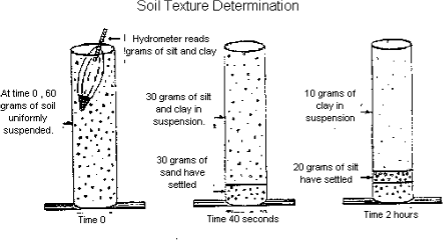
\includegraphics{hydrometer-Picture1.png}

}

\caption{\label{fig-hydrometer}Hydrometer Process}

\end{figure}

(Note: The soil in the diagram has (60-30)/60 x 100= 50\% Sand; 10/60
x100= 17\% Clay; 100-50-17=33\% Silt)

\textbf{Calculations}: correct readings before calculating sand, silt,
and clay!

\[
Sand (\%) = \frac{M_{sample,ovendry} - 40s\ reading}{M_{sample,ovendry}} x 100%
\]

\textbf{Results}

 
  \providecommand{\huxb}[2]{\arrayrulecolor[RGB]{#1}\global\arrayrulewidth=#2pt}
  \providecommand{\huxvb}[2]{\color[RGB]{#1}\vrule width #2pt}
  \providecommand{\huxtpad}[1]{\rule{0pt}{#1}}
  \providecommand{\huxbpad}[1]{\rule[-#1]{0pt}{#1}}

\begin{table}[h!]
\begin{centerbox}
\begin{threeparttable}
 
\setlength{\tabcolsep}{0pt}
\begin{tabularx}{0.9\textwidth}{p{0.3\textwidth} p{0.3\textwidth} p{0.3\textwidth}}


\hhline{>{\huxb{0, 0, 0}{1}}->{\huxb{0, 0, 0}{1}}->{\huxb{0, 0, 0}{1}}-}
\arrayrulecolor{black}

\multicolumn{1}{!{\huxvb{0, 0, 0}{1}}m{0.3\textwidth}!{\huxvb{0, 0, 0}{1}}}{\hspace{0pt}\parbox[c]{0.3\textwidth-0pt-4pt}{\huxtpad{0pt + 1em}\centering \textbf{Measurements}\huxbpad{4pt}}} &
\multicolumn{1}{m{0.3\textwidth}!{\huxvb{0, 0, 0}{1}}}{\hspace{4pt}\parbox[c]{0.3\textwidth-4pt-4pt}{\huxtpad{0pt + 1em}\centering \textbf{Sample 1}\huxbpad{4pt}}} &
\multicolumn{1}{m{0.3\textwidth}!{\huxvb{0, 0, 0}{1}}}{\hspace{4pt}\parbox[c]{0.3\textwidth-4pt-0pt}{\huxtpad{0pt + 1em}\centering \textbf{Sample 2}\huxbpad{4pt}}} \tabularnewline[-0.5pt]


\hhline{>{\huxb{0, 0, 0}{1}}->{\huxb{0, 0, 0}{1}}->{\huxb{0, 0, 0}{1}}-}
\arrayrulecolor{black}

\multicolumn{1}{!{\huxvb{0, 0, 0}{1}}m{0.3\textwidth}!{\huxvb{0, 0, 0}{1}}}{\hspace{0pt}\parbox[c]{0.3\textwidth-0pt-4pt}{\huxtpad{4pt + 1em}\raggedright Sample mass (oven-dry)\huxbpad{4pt}}} &
\multicolumn{1}{m{0.3\textwidth}!{\huxvb{0, 0, 0}{1}}}{\hspace{4pt}\parbox[c]{0.3\textwidth-4pt-4pt}{\huxtpad{4pt + 1em}\raggedleft 60 g\huxbpad{4pt}}} &
\multicolumn{1}{m{0.3\textwidth}!{\huxvb{0, 0, 0}{1}}}{\hspace{4pt}\parbox[c]{0.3\textwidth-4pt-0pt}{\huxtpad{4pt + 1em}\raggedleft 60 g\huxbpad{4pt}}} \tabularnewline[-0.5pt]


\hhline{>{\huxb{0, 0, 0}{1}}->{\huxb{0, 0, 0}{1}}->{\huxb{0, 0, 0}{1}}-}
\arrayrulecolor{black}

\multicolumn{1}{!{\huxvb{0, 0, 0}{1}}m{0.3\textwidth}!{\huxvb{0, 0, 0}{1}}}{\hspace{0pt}\parbox[c]{0.3\textwidth-0pt-4pt}{\huxtpad{4pt + 1em}\raggedright 40s reading (uncorrected\huxbpad{4pt}}} &
\multicolumn{1}{m{0.3\textwidth}!{\huxvb{0, 0, 0}{1}}}{\hspace{4pt}\parbox[c]{0.3\textwidth-4pt-4pt}{\huxtpad{4pt + 1em}\raggedleft g/L\huxbpad{4pt}}} &
\multicolumn{1}{m{0.3\textwidth}!{\huxvb{0, 0, 0}{1}}}{\hspace{4pt}\parbox[c]{0.3\textwidth-4pt-0pt}{\huxtpad{4pt + 1em}\raggedleft g/L\huxbpad{4pt}}} \tabularnewline[-0.5pt]


\hhline{>{\huxb{0, 0, 0}{1}}->{\huxb{0, 0, 0}{1}}->{\huxb{0, 0, 0}{1}}-}
\arrayrulecolor{black}

\multicolumn{1}{!{\huxvb{0, 0, 0}{1}}m{0.3\textwidth}!{\huxvb{0, 0, 0}{1}}}{\hspace{0pt}\parbox[c]{0.3\textwidth-0pt-4pt}{\huxtpad{4pt + 1em}\raggedright Temperature (C)\huxbpad{4pt}}} &
\multicolumn{1}{m{0.3\textwidth}!{\huxvb{0, 0, 0}{1}}}{\hspace{4pt}\parbox[c]{0.3\textwidth-4pt-4pt}{\huxtpad{4pt + 1em}\raggedleft ºC\huxbpad{4pt}}} &
\multicolumn{1}{m{0.3\textwidth}!{\huxvb{0, 0, 0}{1}}}{\hspace{4pt}\parbox[c]{0.3\textwidth-4pt-0pt}{\huxtpad{4pt + 1em}\raggedleft ºC\huxbpad{4pt}}} \tabularnewline[-0.5pt]


\hhline{>{\huxb{0, 0, 0}{1}}->{\huxb{0, 0, 0}{1}}->{\huxb{0, 0, 0}{1}}-}
\arrayrulecolor{black}

\multicolumn{1}{!{\huxvb{0, 0, 0}{1}}m{0.3\textwidth}!{\huxvb{0, 0, 0}{1}}}{\hspace{0pt}\parbox[c]{0.3\textwidth-0pt-4pt}{\huxtpad{4pt + 1em}\raggedright 40s reading (corrected)\huxbpad{4pt}}} &
\multicolumn{1}{m{0.3\textwidth}!{\huxvb{0, 0, 0}{1}}}{\hspace{4pt}\parbox[c]{0.3\textwidth-4pt-4pt}{\huxtpad{4pt + 1em}\raggedleft g/L\huxbpad{4pt}}} &
\multicolumn{1}{m{0.3\textwidth}!{\huxvb{0, 0, 0}{1}}}{\hspace{4pt}\parbox[c]{0.3\textwidth-4pt-0pt}{\huxtpad{4pt + 1em}\raggedleft g/L\huxbpad{4pt}}} \tabularnewline[-0.5pt]


\hhline{>{\huxb{0, 0, 0}{1}}->{\huxb{0, 0, 0}{1}}->{\huxb{0, 0, 0}{1}}-}
\arrayrulecolor{black}

\multicolumn{1}{!{\huxvb{0, 0, 0}{1}}m{0.3\textwidth}!{\huxvb{0, 0, 0}{1}}}{\hspace{0pt}\parbox[c]{0.3\textwidth-0pt-4pt}{\huxtpad{4pt + 1em}\raggedright \% Sand\huxbpad{4pt}}} &
\multicolumn{1}{m{0.3\textwidth}!{\huxvb{0, 0, 0}{1}}}{\hspace{4pt}\parbox[c]{0.3\textwidth-4pt-4pt}{\huxtpad{4pt + 1em}\raggedleft \%\huxbpad{4pt}}} &
\multicolumn{1}{m{0.3\textwidth}!{\huxvb{0, 0, 0}{1}}}{\hspace{4pt}\parbox[c]{0.3\textwidth-4pt-0pt}{\huxtpad{4pt + 1em}\raggedleft \%\huxbpad{4pt}}} \tabularnewline[-0.5pt]


\hhline{>{\huxb{0, 0, 0}{1}}->{\huxb{0, 0, 0}{1}}->{\huxb{0, 0, 0}{1}}-}
\arrayrulecolor{black}

\multicolumn{1}{!{\huxvb{0, 0, 0}{1}}m{0.3\textwidth}!{\huxvb{0, 0, 0}{1}}}{\hspace{0pt}\parbox[c]{0.3\textwidth-0pt-4pt}{\huxtpad{4pt + 1em}\raggedright 2hr reading (uncorrected)\huxbpad{4pt}}} &
\multicolumn{1}{m{0.3\textwidth}!{\huxvb{0, 0, 0}{1}}}{\hspace{4pt}\parbox[c]{0.3\textwidth-4pt-4pt}{\huxtpad{4pt + 1em}\raggedleft g/L\huxbpad{4pt}}} &
\multicolumn{1}{m{0.3\textwidth}!{\huxvb{0, 0, 0}{1}}}{\hspace{4pt}\parbox[c]{0.3\textwidth-4pt-0pt}{\huxtpad{4pt + 1em}\raggedleft g/L\huxbpad{4pt}}} \tabularnewline[-0.5pt]


\hhline{>{\huxb{0, 0, 0}{1}}->{\huxb{0, 0, 0}{1}}->{\huxb{0, 0, 0}{1}}-}
\arrayrulecolor{black}

\multicolumn{1}{!{\huxvb{0, 0, 0}{1}}m{0.3\textwidth}!{\huxvb{0, 0, 0}{1}}}{\hspace{0pt}\parbox[c]{0.3\textwidth-0pt-4pt}{\huxtpad{4pt + 1em}\raggedright Temperature @2hr (C)\huxbpad{4pt}}} &
\multicolumn{1}{m{0.3\textwidth}!{\huxvb{0, 0, 0}{1}}}{\hspace{4pt}\parbox[c]{0.3\textwidth-4pt-4pt}{\huxtpad{4pt + 1em}\raggedleft ºC\huxbpad{4pt}}} &
\multicolumn{1}{m{0.3\textwidth}!{\huxvb{0, 0, 0}{1}}}{\hspace{4pt}\parbox[c]{0.3\textwidth-4pt-0pt}{\huxtpad{4pt + 1em}\raggedleft ºC\huxbpad{4pt}}} \tabularnewline[-0.5pt]


\hhline{>{\huxb{0, 0, 0}{1}}->{\huxb{0, 0, 0}{1}}->{\huxb{0, 0, 0}{1}}-}
\arrayrulecolor{black}

\multicolumn{1}{!{\huxvb{0, 0, 0}{1}}m{0.3\textwidth}!{\huxvb{0, 0, 0}{1}}}{\hspace{0pt}\parbox[c]{0.3\textwidth-0pt-4pt}{\huxtpad{4pt + 1em}\raggedright 2hr readng (corrected)\huxbpad{4pt}}} &
\multicolumn{1}{m{0.3\textwidth}!{\huxvb{0, 0, 0}{1}}}{\hspace{4pt}\parbox[c]{0.3\textwidth-4pt-4pt}{\huxtpad{4pt + 1em}\raggedleft g/L\huxbpad{4pt}}} &
\multicolumn{1}{m{0.3\textwidth}!{\huxvb{0, 0, 0}{1}}}{\hspace{4pt}\parbox[c]{0.3\textwidth-4pt-0pt}{\huxtpad{4pt + 1em}\raggedleft g/L\huxbpad{4pt}}} \tabularnewline[-0.5pt]


\hhline{>{\huxb{0, 0, 0}{1}}->{\huxb{0, 0, 0}{1}}->{\huxb{0, 0, 0}{1}}-}
\arrayrulecolor{black}

\multicolumn{1}{!{\huxvb{0, 0, 0}{1}}m{0.3\textwidth}!{\huxvb{0, 0, 0}{1}}}{\hspace{0pt}\parbox[c]{0.3\textwidth-0pt-4pt}{\huxtpad{4pt + 1em}\raggedright \% Clay\huxbpad{4pt}}} &
\multicolumn{1}{m{0.3\textwidth}!{\huxvb{0, 0, 0}{1}}}{\hspace{4pt}\parbox[c]{0.3\textwidth-4pt-4pt}{\huxtpad{4pt + 1em}\raggedleft \%\huxbpad{4pt}}} &
\multicolumn{1}{m{0.3\textwidth}!{\huxvb{0, 0, 0}{1}}}{\hspace{4pt}\parbox[c]{0.3\textwidth-4pt-0pt}{\huxtpad{4pt + 1em}\raggedleft \%\huxbpad{4pt}}} \tabularnewline[-0.5pt]


\hhline{>{\huxb{0, 0, 0}{1}}->{\huxb{0, 0, 0}{1}}->{\huxb{0, 0, 0}{1}}-}
\arrayrulecolor{black}

\multicolumn{1}{!{\huxvb{0, 0, 0}{1}}m{0.3\textwidth}!{\huxvb{0, 0, 0}{1}}}{\hspace{0pt}\parbox[c]{0.3\textwidth-0pt-4pt}{\huxtpad{4pt + 1em}\raggedright \% Silt\huxbpad{0pt}}} &
\multicolumn{1}{m{0.3\textwidth}!{\huxvb{0, 0, 0}{1}}}{\hspace{4pt}\parbox[c]{0.3\textwidth-4pt-4pt}{\huxtpad{4pt + 1em}\raggedleft \%\huxbpad{0pt}}} &
\multicolumn{1}{m{0.3\textwidth}!{\huxvb{0, 0, 0}{1}}}{\hspace{4pt}\parbox[c]{0.3\textwidth-4pt-0pt}{\huxtpad{4pt + 1em}\raggedleft \%\huxbpad{0pt}}} \tabularnewline[-0.5pt]


\hhline{>{\huxb{0, 0, 0}{1}}->{\huxb{0, 0, 0}{1}}->{\huxb{0, 0, 0}{1}}-}
\arrayrulecolor{black}
\end{tabularx}
\end{threeparttable}\par\end{centerbox}

\end{table}
 

 
  \providecommand{\huxb}[2]{\arrayrulecolor[RGB]{#1}\global\arrayrulewidth=#2pt}
  \providecommand{\huxvb}[2]{\color[RGB]{#1}\vrule width #2pt}
  \providecommand{\huxtpad}[1]{\rule{0pt}{#1}}
  \providecommand{\huxbpad}[1]{\rule[-#1]{0pt}{#1}}

\begin{table}[h!]
\begin{centerbox}
\begin{threeparttable}
 
\setlength{\tabcolsep}{0pt}
\begin{tabularx}{0.9\textwidth}{p{0.3\textwidth} p{0.3\textwidth} p{0.3\textwidth}}


\hhline{>{\huxb{0, 0, 0}{1}}->{\huxb{0, 0, 0}{1}}->{\huxb{0, 0, 0}{1}}-}
\arrayrulecolor{black}

\multicolumn{1}{!{\huxvb{0, 0, 0}{1}}m{0.3\textwidth}!{\huxvb{0, 0, 0}{1}}}{\hspace{0pt}\parbox[c]{0.3\textwidth-0pt-4pt}{\huxtpad{0pt + 1em}\centering \textbf{Summary}\huxbpad{4pt}}} &
\multicolumn{1}{m{0.3\textwidth}!{\huxvb{0, 0, 0}{1}}}{\hspace{4pt}\parbox[c]{0.3\textwidth-4pt-4pt}{\huxtpad{0pt + 1em}\centering \textbf{Sample 1}\huxbpad{4pt}}} &
\multicolumn{1}{m{0.3\textwidth}!{\huxvb{0, 0, 0}{1}}}{\hspace{4pt}\parbox[c]{0.3\textwidth-4pt-0pt}{\huxtpad{0pt + 1em}\centering \textbf{Sample 2}\huxbpad{4pt}}} \tabularnewline[-0.5pt]


\hhline{>{\huxb{0, 0, 0}{1}}->{\huxb{0, 0, 0}{1}}->{\huxb{0, 0, 0}{1}}-}
\arrayrulecolor{black}

\multicolumn{1}{!{\huxvb{0, 0, 0}{1}}m{0.3\textwidth}!{\huxvb{0, 0, 0}{1}}}{\hspace{0pt}\parbox[c]{0.3\textwidth-0pt-4pt}{\huxtpad{4pt + 1em}\centering \% sand\huxbpad{4pt}}} &
\multicolumn{1}{m{0.3\textwidth}!{\huxvb{0, 0, 0}{1}}}{\hspace{4pt}\parbox[c]{0.3\textwidth-4pt-4pt}{\huxtpad{4pt + 1em}\centering \huxbpad{4pt}}} &
\multicolumn{1}{m{0.3\textwidth}!{\huxvb{0, 0, 0}{1}}}{\hspace{4pt}\parbox[c]{0.3\textwidth-4pt-0pt}{\huxtpad{4pt + 1em}\centering \huxbpad{4pt}}} \tabularnewline[-0.5pt]


\hhline{>{\huxb{0, 0, 0}{1}}->{\huxb{0, 0, 0}{1}}->{\huxb{0, 0, 0}{1}}-}
\arrayrulecolor{black}

\multicolumn{1}{!{\huxvb{0, 0, 0}{1}}m{0.3\textwidth}!{\huxvb{0, 0, 0}{1}}}{\hspace{0pt}\parbox[c]{0.3\textwidth-0pt-4pt}{\huxtpad{4pt + 1em}\centering \% silt\huxbpad{4pt}}} &
\multicolumn{1}{m{0.3\textwidth}!{\huxvb{0, 0, 0}{1}}}{\hspace{4pt}\parbox[c]{0.3\textwidth-4pt-4pt}{\huxtpad{4pt + 1em}\centering \huxbpad{4pt}}} &
\multicolumn{1}{m{0.3\textwidth}!{\huxvb{0, 0, 0}{1}}}{\hspace{4pt}\parbox[c]{0.3\textwidth-4pt-0pt}{\huxtpad{4pt + 1em}\centering \huxbpad{4pt}}} \tabularnewline[-0.5pt]


\hhline{>{\huxb{0, 0, 0}{1}}->{\huxb{0, 0, 0}{1}}->{\huxb{0, 0, 0}{1}}-}
\arrayrulecolor{black}

\multicolumn{1}{!{\huxvb{0, 0, 0}{1}}m{0.3\textwidth}!{\huxvb{0, 0, 0}{1}}}{\hspace{0pt}\parbox[c]{0.3\textwidth-0pt-4pt}{\huxtpad{4pt + 1em}\centering \% clay\huxbpad{0pt}}} &
\multicolumn{1}{m{0.3\textwidth}!{\huxvb{0, 0, 0}{1}}}{\hspace{4pt}\parbox[c]{0.3\textwidth-4pt-4pt}{\huxtpad{4pt + 1em}\centering \huxbpad{0pt}}} &
\multicolumn{1}{m{0.3\textwidth}!{\huxvb{0, 0, 0}{1}}}{\hspace{4pt}\parbox[c]{0.3\textwidth-4pt-0pt}{\huxtpad{4pt + 1em}\centering \huxbpad{0pt}}} \tabularnewline[-0.5pt]


\hhline{>{\huxb{0, 0, 0}{1}}->{\huxb{0, 0, 0}{1}}->{\huxb{0, 0, 0}{1}}-}
\arrayrulecolor{black}
\end{tabularx}
\end{threeparttable}\par\end{centerbox}

\end{table}
 

\hypertarget{investigation-b-using-the-texture-triangle}{%
\section{INVESTIGATION B: Using the Texture
Triangle}\label{investigation-b-using-the-texture-triangle}}

A soil's textural class is determined by that soil's respective content
of sand, silt, and clay. The USDA textural triangle is used to classify
the texture class of a soil. The sides of the soil textural triangle are
scaled for the percentages of sand, silt, and clay (0-100\%). Clay
percentages are read along the lines from left to right across the
triangle. Silt is read along the lines from the upper right to lower
left. Sand along the lines from lower right to the upper left portion of
the triangle. The intersections of the three sides on the triangle give
the texture class name. For instance, if you have a soil with 20\% clay,
45\% silt, and 35\% sand, it would fall in the ``loam'' textural class
name.

\begin{figure}

{\centering 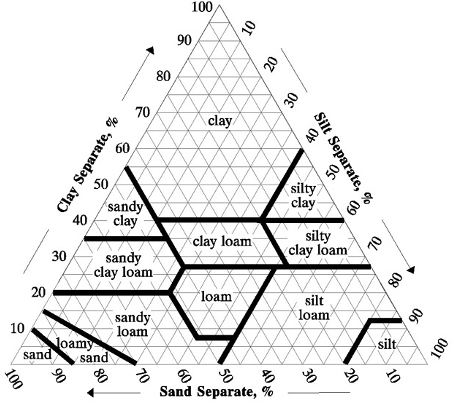
\includegraphics{texture-triangle-Picture1.png}

}

\caption{\label{fig-triangle}USDA Soil Texture Triangle}

\end{figure}

\textbf{Results}

Using the soil particle percent data from Investigation A, determine the
texture class for the soil samples 1 and 2.

 
  \providecommand{\huxb}[2]{\arrayrulecolor[RGB]{#1}\global\arrayrulewidth=#2pt}
  \providecommand{\huxvb}[2]{\color[RGB]{#1}\vrule width #2pt}
  \providecommand{\huxtpad}[1]{\rule{0pt}{#1}}
  \providecommand{\huxbpad}[1]{\rule[-#1]{0pt}{#1}}

\begin{table}[h!]
\begin{centerbox}
\begin{threeparttable}
 
\setlength{\tabcolsep}{0pt}
\begin{tabularx}{0.9\textwidth}{p{0.18\textwidth} p{0.18\textwidth} p{0.18\textwidth} p{0.18\textwidth} p{0.18\textwidth}}


\hhline{>{\huxb{0, 0, 0}{1}}->{\huxb{0, 0, 0}{1}}->{\huxb{0, 0, 0}{1}}->{\huxb{0, 0, 0}{1}}->{\huxb{0, 0, 0}{1}}-}
\arrayrulecolor{black}

\multicolumn{1}{!{\huxvb{0, 0, 0}{1}}m{0.18\textwidth}!{\huxvb{0, 0, 0}{1}}}{\hspace{0pt}\parbox[c]{0.18\textwidth-0pt-4pt}{\huxtpad{0pt + 1em}\centering \textbf{Sample}\huxbpad{4pt}}} &
\multicolumn{1}{m{0.18\textwidth}!{\huxvb{0, 0, 0}{1}}}{\hspace{4pt}\parbox[c]{0.18\textwidth-4pt-4pt}{\huxtpad{0pt + 1em}\centering \textbf{Sand \%}\huxbpad{4pt}}} &
\multicolumn{1}{m{0.18\textwidth}!{\huxvb{0, 0, 0}{1}}}{\hspace{4pt}\parbox[c]{0.18\textwidth-4pt-4pt}{\huxtpad{0pt + 1em}\centering \textbf{Silt \%}\huxbpad{4pt}}} &
\multicolumn{1}{m{0.18\textwidth}!{\huxvb{0, 0, 0}{1}}}{\hspace{4pt}\parbox[c]{0.18\textwidth-4pt-4pt}{\huxtpad{0pt + 1em}\centering \textbf{Clay \%}\huxbpad{4pt}}} &
\multicolumn{1}{m{0.18\textwidth}!{\huxvb{0, 0, 0}{1}}}{\hspace{4pt}\parbox[c]{0.18\textwidth-4pt-0pt}{\huxtpad{0pt + 1em}\centering \textbf{Texture Class}\huxbpad{4pt}}} \tabularnewline[-0.5pt]


\hhline{>{\huxb{0, 0, 0}{1}}->{\huxb{0, 0, 0}{1}}->{\huxb{0, 0, 0}{1}}->{\huxb{0, 0, 0}{1}}->{\huxb{0, 0, 0}{1}}-}
\arrayrulecolor{black}

\multicolumn{1}{!{\huxvb{0, 0, 0}{1}}m{0.18\textwidth}!{\huxvb{0, 0, 0}{1}}}{\hspace{0pt}\parbox[c]{0.18\textwidth-0pt-4pt}{\huxtpad{20pt + 1em}\centering 1\huxbpad{20pt}}} &
\multicolumn{1}{m{0.18\textwidth}!{\huxvb{0, 0, 0}{1}}}{\hspace{4pt}\parbox[c]{0.18\textwidth-4pt-4pt}{\huxtpad{20pt + 1em}\centering \huxbpad{20pt}}} &
\multicolumn{1}{m{0.18\textwidth}!{\huxvb{0, 0, 0}{1}}}{\hspace{4pt}\parbox[c]{0.18\textwidth-4pt-4pt}{\huxtpad{20pt + 1em}\centering \huxbpad{20pt}}} &
\multicolumn{1}{m{0.18\textwidth}!{\huxvb{0, 0, 0}{1}}}{\hspace{4pt}\parbox[c]{0.18\textwidth-4pt-4pt}{\huxtpad{20pt + 1em}\centering \huxbpad{20pt}}} &
\multicolumn{1}{m{0.18\textwidth}!{\huxvb{0, 0, 0}{1}}}{\hspace{4pt}\parbox[c]{0.18\textwidth-4pt-0pt}{\huxtpad{20pt + 1em}\centering \huxbpad{20pt}}} \tabularnewline[-0.5pt]


\hhline{>{\huxb{0, 0, 0}{1}}->{\huxb{0, 0, 0}{1}}->{\huxb{0, 0, 0}{1}}->{\huxb{0, 0, 0}{1}}->{\huxb{0, 0, 0}{1}}-}
\arrayrulecolor{black}

\multicolumn{1}{!{\huxvb{0, 0, 0}{1}}m{0.18\textwidth}!{\huxvb{0, 0, 0}{1}}}{\hspace{0pt}\parbox[c]{0.18\textwidth-0pt-4pt}{\huxtpad{20pt + 1em}\centering 2\huxbpad{20pt}}} &
\multicolumn{1}{m{0.18\textwidth}!{\huxvb{0, 0, 0}{1}}}{\hspace{4pt}\parbox[c]{0.18\textwidth-4pt-4pt}{\huxtpad{20pt + 1em}\centering \huxbpad{20pt}}} &
\multicolumn{1}{m{0.18\textwidth}!{\huxvb{0, 0, 0}{1}}}{\hspace{4pt}\parbox[c]{0.18\textwidth-4pt-4pt}{\huxtpad{20pt + 1em}\centering \huxbpad{20pt}}} &
\multicolumn{1}{m{0.18\textwidth}!{\huxvb{0, 0, 0}{1}}}{\hspace{4pt}\parbox[c]{0.18\textwidth-4pt-4pt}{\huxtpad{20pt + 1em}\centering \huxbpad{20pt}}} &
\multicolumn{1}{m{0.18\textwidth}!{\huxvb{0, 0, 0}{1}}}{\hspace{4pt}\parbox[c]{0.18\textwidth-4pt-0pt}{\huxtpad{20pt + 1em}\centering \huxbpad{20pt}}} \tabularnewline[-0.5pt]


\hhline{>{\huxb{0, 0, 0}{1}}->{\huxb{0, 0, 0}{1}}->{\huxb{0, 0, 0}{1}}->{\huxb{0, 0, 0}{1}}->{\huxb{0, 0, 0}{1}}-}
\arrayrulecolor{black}
\end{tabularx}
\end{threeparttable}\par\end{centerbox}

\end{table}
 

\hypertarget{investigation-c-texturing-soil-with-the-feel-method}{%
\section{INVESTIGATION C: Texturing Soil with the ``Feel''
Method}\label{investigation-c-texturing-soil-with-the-feel-method}}

Determining texture by feel takes practice (professional soil scientists
can texture soil by feel and determine the texture within five percent
clay content!). The following table, chart provided in lab, and text
will help you learn how to texture by feel.

 
  \providecommand{\huxb}[2]{\arrayrulecolor[RGB]{#1}\global\arrayrulewidth=#2pt}
  \providecommand{\huxvb}[2]{\color[RGB]{#1}\vrule width #2pt}
  \providecommand{\huxtpad}[1]{\rule{0pt}{#1}}
  \providecommand{\huxbpad}[1]{\rule[-#1]{0pt}{#1}}

\begin{table}[h!]
\begin{centerbox}
\begin{threeparttable}
 
\setlength{\tabcolsep}{0pt}
\begin{tabularx}{0.9\textwidth}{p{0.45\textwidth} p{0.45\textwidth}}


\hhline{>{\huxb{0, 0, 0}{1}}->{\huxb{0, 0, 0}{1}}-}
\arrayrulecolor{black}

\multicolumn{1}{!{\huxvb{0, 0, 0}{1}}m{0.45\textwidth}!{\huxvb{0, 0, 0}{1}}}{\hspace{0pt}\parbox[c]{0.45\textwidth-0pt-4pt}{\huxtpad{0pt + 1em}\centering \textbf{Texture}\huxbpad{4pt}}} &
\multicolumn{1}{m{0.45\textwidth}!{\huxvb{0, 0, 0}{1}}}{\hspace{4pt}\parbox[c]{0.45\textwidth-4pt-0pt}{\huxtpad{0pt + 1em}\centering \textbf{Feel}\huxbpad{4pt}}} \tabularnewline[-0.5pt]


\hhline{>{\huxb{0, 0, 0}{1}}->{\huxb{0, 0, 0}{1}}-}
\arrayrulecolor{black}

\multicolumn{1}{!{\huxvb{0, 0, 0}{1}}m{0.45\textwidth}!{\huxvb{0, 0, 0}{1}}}{\hspace{0pt}\parbox[c]{0.45\textwidth-0pt-4pt}{\huxtpad{4pt + 1em}\centering Coarse sand\huxbpad{4pt}}} &
\multicolumn{1}{m{0.45\textwidth}!{\huxvb{0, 0, 0}{1}}}{\hspace{4pt}\parbox[c]{0.45\textwidth-4pt-0pt}{\huxtpad{4pt + 1em}\centering Feels sharp, rasping, gritty, individual grains easily distinguished.\huxbpad{4pt}}} \tabularnewline[-0.5pt]


\hhline{>{\huxb{0, 0, 0}{1}}->{\huxb{0, 0, 0}{1}}-}
\arrayrulecolor{black}

\multicolumn{1}{!{\huxvb{0, 0, 0}{1}}m{0.45\textwidth}!{\huxvb{0, 0, 0}{1}}}{\hspace{0pt}\parbox[c]{0.45\textwidth-0pt-4pt}{\huxtpad{4pt + 1em}\centering Fine sand\huxbpad{4pt}}} &
\multicolumn{1}{m{0.45\textwidth}!{\huxvb{0, 0, 0}{1}}}{\hspace{4pt}\parbox[c]{0.45\textwidth-4pt-0pt}{\huxtpad{4pt + 1em}\centering Gritty but very fine. Individual grains only just visible. Rasping sound between finger and thumb heard when placed close to the ear.\huxbpad{4pt}}} \tabularnewline[-0.5pt]


\hhline{>{\huxb{0, 0, 0}{1}}->{\huxb{0, 0, 0}{1}}-}
\arrayrulecolor{black}

\multicolumn{1}{!{\huxvb{0, 0, 0}{1}}m{0.45\textwidth}!{\huxvb{0, 0, 0}{1}}}{\hspace{0pt}\parbox[c]{0.45\textwidth-0pt-4pt}{\huxtpad{4pt + 1em}\centering Silt\huxbpad{4pt}}} &
\multicolumn{1}{m{0.45\textwidth}!{\huxvb{0, 0, 0}{1}}}{\hspace{4pt}\parbox[c]{0.45\textwidth-4pt-0pt}{\huxtpad{4pt + 1em}\centering Dry pellets will crush between the fingers, yielding a floury dust with a smooth silky feel. When wet, the silkiness persists and the cast is slightly plastic (not \newline very sticky). Particles are not quite visible to the naked eye.\huxbpad{4pt}}} \tabularnewline[-0.5pt]


\hhline{>{\huxb{0, 0, 0}{1}}->{\huxb{0, 0, 0}{1}}-}
\arrayrulecolor{black}

\multicolumn{1}{!{\huxvb{0, 0, 0}{1}}m{0.45\textwidth}!{\huxvb{0, 0, 0}{1}}}{\hspace{0pt}\parbox[c]{0.45\textwidth-0pt-4pt}{\huxtpad{4pt + 1em}\centering Clay\huxbpad{0pt}}} &
\multicolumn{1}{m{0.45\textwidth}!{\huxvb{0, 0, 0}{1}}}{\hspace{4pt}\parbox[c]{0.45\textwidth-4pt-0pt}{\huxtpad{4pt + 1em}\centering Dry pellets feel very hard, and it is difficult or impossible to crush them between the finger and thumb. When moistened, it is very sticky (plastic-like consistency).\huxbpad{0pt}}} \tabularnewline[-0.5pt]


\hhline{>{\huxb{0, 0, 0}{1}}->{\huxb{0, 0, 0}{1}}-}
\arrayrulecolor{black}
\end{tabularx}
\end{threeparttable}\par\end{centerbox}

\end{table}
 

\textbf{WATCH VIDEO TUTORIAL ON IPADS!}

\begin{enumerate}
\def\labelenumi{\arabic{enumi}.}
\item
  To determine the soil texture by feel, the soil must be moistened. Add
  a small amount of water to the soil if needed to give it a putty-like
  (play-doh) consistency. Not too wet - not too dry!
\item
  Form the soil into a ball.
\item
  Try to push the soil between your thumb and forefinger to make a
  ``ribbon'' \textasciitilde{} 2mm thick; the longer the ribbon, the
  more clay there is in the soil.
\item
  Move the soil between your thumb and forefinger to determine if the
  soil feels really gritty, really smooth, or somewhere in between. Sand
  feels gritty, silt feels smooth, clay feels sticky (allows you to form
  ribbons).
\item
  Use the provided flow chart and suggested order below to assist in
  calibrating yourself.
\end{enumerate}

\textbf{Practicing -- WASH YOUR HANDS BETWEEN EVERY SAMPLE!!!!!!!} Use
the known texture samples to practice texturing soil with the ``feel''
method.

Here is a suggested method of practicing (Nic's method to the madness):

\begin{enumerate}
\def\labelenumi{\arabic{enumi}.}
\item
  Start with the silt loam -- you should be able to make a ribbon, but
  \textless{} 1''
\item
  Move to the silty clay loam -- you should notice that you can get a
  longer ribbon, 1-2''
\item
  Move to the silty clay -- you should be able to get an even longer
  ribbon, \textgreater{} 2''
\item
  In these three samples, you kept increasing clay content while
  decreasing sand content.
\item
  Now try the loam -- you should notice that it feels like there is more
  sand in it than in the silt loam, silty clay loam and silty clay, but
  it doesn't feel really gritty. The loam texture class should feel like
  equal proportions of sand, silt and clay. You should be able to make a
  ribbon, but \textless{} 1''.
\item
  Move to the loamy sand. This should feel much grittier and you
  shouldn't be able to make a ribbon. However, the soil should form a
  ball without being excessively wet.
\item
  Finally move to the sand. This should feel extremely gritty and you
  shouldn't be able to make a ribbon. You need to get sands excessively
  wet in order make a ball out of them.
\item
  Lastly, try moving from the loam to the clay loam and finally the
  clay. You should feel a clay increase similar to the silt loam to
  silty clay loam to silty clay samples, but since these all have more
  sand, they should feel less smooth and more like a mixture of the
  particle size classes.
\end{enumerate}

\textbf{Note}: Check one box to choose between the characteristics
(gritty, smooth, or gritty/smooth). For ribbon length, choose between
short (\textless1''), medium (1-2''), or long (\textgreater2'').

 
  \providecommand{\huxb}[2]{\arrayrulecolor[RGB]{#1}\global\arrayrulewidth=#2pt}
  \providecommand{\huxvb}[2]{\color[RGB]{#1}\vrule width #2pt}
  \providecommand{\huxtpad}[1]{\rule{0pt}{#1}}
  \providecommand{\huxbpad}[1]{\rule[-#1]{0pt}{#1}}

\begin{table}[h!]
\begin{centerbox}
\begin{threeparttable}
 
\setlength{\tabcolsep}{0pt}
\begin{tabularx}{0.9\textwidth}{p{0.18\textwidth} p{0.18\textwidth} p{0.18\textwidth} p{0.18\textwidth} p{0.18\textwidth}}


\hhline{>{\huxb{0, 0, 0}{1}}->{\huxb{0, 0, 0}{1}}->{\huxb{0, 0, 0}{1}}->{\huxb{0, 0, 0}{1}}->{\huxb{0, 0, 0}{1}}-}
\arrayrulecolor{black}

\multicolumn{1}{!{\huxvb{0, 0, 0}{1}}m{0.18\textwidth}!{\huxvb{0, 0, 0}{1}}}{\hspace{0pt}\parbox[c]{0.18\textwidth-0pt-4pt}{\huxtpad{0pt + 1em}\centering \textbf{Texture}\huxbpad{4pt}}} &
\multicolumn{1}{m{0.18\textwidth}!{\huxvb{0, 0, 0}{1}}}{\hspace{4pt}\parbox[c]{0.18\textwidth-4pt-4pt}{\huxtpad{0pt + 1em}\centering \textbf{Dominated by gritty feel}\huxbpad{4pt}}} &
\multicolumn{1}{m{0.18\textwidth}!{\huxvb{0, 0, 0}{1}}}{\hspace{4pt}\parbox[c]{0.18\textwidth-4pt-4pt}{\huxtpad{0pt + 1em}\centering \textbf{Dominated by smooth feel}\huxbpad{4pt}}} &
\multicolumn{1}{m{0.18\textwidth}!{\huxvb{0, 0, 0}{1}}}{\hspace{4pt}\parbox[c]{0.18\textwidth-4pt-4pt}{\huxtpad{0pt + 1em}\centering \textbf{Equally gritty/smooth}\huxbpad{4pt}}} &
\multicolumn{1}{m{0.18\textwidth}!{\huxvb{0, 0, 0}{1}}}{\hspace{4pt}\parbox[c]{0.18\textwidth-4pt-0pt}{\huxtpad{0pt + 1em}\centering \textbf{Ribbon length}\huxbpad{4pt}}} \tabularnewline[-0.5pt]


\hhline{>{\huxb{0, 0, 0}{1}}->{\huxb{0, 0, 0}{1}}->{\huxb{0, 0, 0}{1}}->{\huxb{0, 0, 0}{1}}->{\huxb{0, 0, 0}{1}}-}
\arrayrulecolor{black}

\multicolumn{1}{!{\huxvb{0, 0, 0}{1}}m{0.18\textwidth}!{\huxvb{0, 0, 0}{1}}}{\hspace{0pt}\parbox[c]{0.18\textwidth-0pt-4pt}{\huxtpad{4pt + 1em}\centering Silt Loam\huxbpad{20pt}}} &
\multicolumn{1}{m{0.18\textwidth}!{\huxvb{0, 0, 0}{1}}}{\hspace{4pt}\parbox[c]{0.18\textwidth-4pt-4pt}{\huxtpad{4pt + 1em}\centering \huxbpad{20pt}}} &
\multicolumn{1}{m{0.18\textwidth}!{\huxvb{0, 0, 0}{1}}}{\hspace{4pt}\parbox[c]{0.18\textwidth-4pt-4pt}{\huxtpad{4pt + 1em}\centering \huxbpad{20pt}}} &
\multicolumn{1}{m{0.18\textwidth}!{\huxvb{0, 0, 0}{1}}}{\hspace{4pt}\parbox[c]{0.18\textwidth-4pt-4pt}{\huxtpad{4pt + 1em}\centering \huxbpad{20pt}}} &
\multicolumn{1}{m{0.18\textwidth}!{\huxvb{0, 0, 0}{1}}}{\hspace{4pt}\parbox[c]{0.18\textwidth-4pt-0pt}{\huxtpad{4pt + 1em}\centering \huxbpad{20pt}}} \tabularnewline[-0.5pt]


\hhline{>{\huxb{0, 0, 0}{1}}->{\huxb{0, 0, 0}{1}}->{\huxb{0, 0, 0}{1}}->{\huxb{0, 0, 0}{1}}->{\huxb{0, 0, 0}{1}}-}
\arrayrulecolor{black}

\multicolumn{1}{!{\huxvb{0, 0, 0}{1}}m{0.18\textwidth}!{\huxvb{0, 0, 0}{1}}}{\hspace{0pt}\parbox[c]{0.18\textwidth-0pt-4pt}{\huxtpad{4pt + 1em}\centering Silty Clay Loam\huxbpad{20pt}}} &
\multicolumn{1}{m{0.18\textwidth}!{\huxvb{0, 0, 0}{1}}}{\hspace{4pt}\parbox[c]{0.18\textwidth-4pt-4pt}{\huxtpad{4pt + 1em}\centering \huxbpad{20pt}}} &
\multicolumn{1}{m{0.18\textwidth}!{\huxvb{0, 0, 0}{1}}}{\hspace{4pt}\parbox[c]{0.18\textwidth-4pt-4pt}{\huxtpad{4pt + 1em}\centering \huxbpad{20pt}}} &
\multicolumn{1}{m{0.18\textwidth}!{\huxvb{0, 0, 0}{1}}}{\hspace{4pt}\parbox[c]{0.18\textwidth-4pt-4pt}{\huxtpad{4pt + 1em}\centering \huxbpad{20pt}}} &
\multicolumn{1}{m{0.18\textwidth}!{\huxvb{0, 0, 0}{1}}}{\hspace{4pt}\parbox[c]{0.18\textwidth-4pt-0pt}{\huxtpad{4pt + 1em}\centering \huxbpad{20pt}}} \tabularnewline[-0.5pt]


\hhline{>{\huxb{0, 0, 0}{1}}->{\huxb{0, 0, 0}{1}}->{\huxb{0, 0, 0}{1}}->{\huxb{0, 0, 0}{1}}->{\huxb{0, 0, 0}{1}}-}
\arrayrulecolor{black}

\multicolumn{1}{!{\huxvb{0, 0, 0}{1}}m{0.18\textwidth}!{\huxvb{0, 0, 0}{1}}}{\hspace{0pt}\parbox[c]{0.18\textwidth-0pt-4pt}{\huxtpad{4pt + 1em}\centering Silty Clay\huxbpad{20pt}}} &
\multicolumn{1}{m{0.18\textwidth}!{\huxvb{0, 0, 0}{1}}}{\hspace{4pt}\parbox[c]{0.18\textwidth-4pt-4pt}{\huxtpad{4pt + 1em}\centering \huxbpad{20pt}}} &
\multicolumn{1}{m{0.18\textwidth}!{\huxvb{0, 0, 0}{1}}}{\hspace{4pt}\parbox[c]{0.18\textwidth-4pt-4pt}{\huxtpad{4pt + 1em}\centering \huxbpad{20pt}}} &
\multicolumn{1}{m{0.18\textwidth}!{\huxvb{0, 0, 0}{1}}}{\hspace{4pt}\parbox[c]{0.18\textwidth-4pt-4pt}{\huxtpad{4pt + 1em}\centering \huxbpad{20pt}}} &
\multicolumn{1}{m{0.18\textwidth}!{\huxvb{0, 0, 0}{1}}}{\hspace{4pt}\parbox[c]{0.18\textwidth-4pt-0pt}{\huxtpad{4pt + 1em}\centering \huxbpad{20pt}}} \tabularnewline[-0.5pt]


\hhline{>{\huxb{0, 0, 0}{1}}->{\huxb{0, 0, 0}{1}}->{\huxb{0, 0, 0}{1}}->{\huxb{0, 0, 0}{1}}->{\huxb{0, 0, 0}{1}}-}
\arrayrulecolor{black}

\multicolumn{1}{!{\huxvb{0, 0, 0}{1}}m{0.18\textwidth}!{\huxvb{0, 0, 0}{1}}}{\hspace{0pt}\parbox[c]{0.18\textwidth-0pt-4pt}{\huxtpad{4pt + 1em}\centering Loam\huxbpad{20pt}}} &
\multicolumn{1}{m{0.18\textwidth}!{\huxvb{0, 0, 0}{1}}}{\hspace{4pt}\parbox[c]{0.18\textwidth-4pt-4pt}{\huxtpad{4pt + 1em}\centering \huxbpad{20pt}}} &
\multicolumn{1}{m{0.18\textwidth}!{\huxvb{0, 0, 0}{1}}}{\hspace{4pt}\parbox[c]{0.18\textwidth-4pt-4pt}{\huxtpad{4pt + 1em}\centering \huxbpad{20pt}}} &
\multicolumn{1}{m{0.18\textwidth}!{\huxvb{0, 0, 0}{1}}}{\hspace{4pt}\parbox[c]{0.18\textwidth-4pt-4pt}{\huxtpad{4pt + 1em}\centering \huxbpad{20pt}}} &
\multicolumn{1}{m{0.18\textwidth}!{\huxvb{0, 0, 0}{1}}}{\hspace{4pt}\parbox[c]{0.18\textwidth-4pt-0pt}{\huxtpad{4pt + 1em}\centering \huxbpad{20pt}}} \tabularnewline[-0.5pt]


\hhline{>{\huxb{0, 0, 0}{1}}->{\huxb{0, 0, 0}{1}}->{\huxb{0, 0, 0}{1}}->{\huxb{0, 0, 0}{1}}->{\huxb{0, 0, 0}{1}}-}
\arrayrulecolor{black}

\multicolumn{1}{!{\huxvb{0, 0, 0}{1}}m{0.18\textwidth}!{\huxvb{0, 0, 0}{1}}}{\hspace{0pt}\parbox[c]{0.18\textwidth-0pt-4pt}{\huxtpad{4pt + 1em}\centering Loamy Sand\huxbpad{20pt}}} &
\multicolumn{1}{m{0.18\textwidth}!{\huxvb{0, 0, 0}{1}}}{\hspace{4pt}\parbox[c]{0.18\textwidth-4pt-4pt}{\huxtpad{4pt + 1em}\centering \huxbpad{20pt}}} &
\multicolumn{1}{m{0.18\textwidth}!{\huxvb{0, 0, 0}{1}}}{\hspace{4pt}\parbox[c]{0.18\textwidth-4pt-4pt}{\huxtpad{4pt + 1em}\centering \huxbpad{20pt}}} &
\multicolumn{1}{m{0.18\textwidth}!{\huxvb{0, 0, 0}{1}}}{\hspace{4pt}\parbox[c]{0.18\textwidth-4pt-4pt}{\huxtpad{4pt + 1em}\centering \huxbpad{20pt}}} &
\multicolumn{1}{m{0.18\textwidth}!{\huxvb{0, 0, 0}{1}}}{\hspace{4pt}\parbox[c]{0.18\textwidth-4pt-0pt}{\huxtpad{4pt + 1em}\centering \huxbpad{20pt}}} \tabularnewline[-0.5pt]


\hhline{>{\huxb{0, 0, 0}{1}}->{\huxb{0, 0, 0}{1}}->{\huxb{0, 0, 0}{1}}->{\huxb{0, 0, 0}{1}}->{\huxb{0, 0, 0}{1}}-}
\arrayrulecolor{black}

\multicolumn{1}{!{\huxvb{0, 0, 0}{1}}m{0.18\textwidth}!{\huxvb{0, 0, 0}{1}}}{\hspace{0pt}\parbox[c]{0.18\textwidth-0pt-4pt}{\huxtpad{4pt + 1em}\centering Sand\huxbpad{20pt}}} &
\multicolumn{1}{m{0.18\textwidth}!{\huxvb{0, 0, 0}{1}}}{\hspace{4pt}\parbox[c]{0.18\textwidth-4pt-4pt}{\huxtpad{4pt + 1em}\centering \huxbpad{20pt}}} &
\multicolumn{1}{m{0.18\textwidth}!{\huxvb{0, 0, 0}{1}}}{\hspace{4pt}\parbox[c]{0.18\textwidth-4pt-4pt}{\huxtpad{4pt + 1em}\centering \huxbpad{20pt}}} &
\multicolumn{1}{m{0.18\textwidth}!{\huxvb{0, 0, 0}{1}}}{\hspace{4pt}\parbox[c]{0.18\textwidth-4pt-4pt}{\huxtpad{4pt + 1em}\centering \huxbpad{20pt}}} &
\multicolumn{1}{m{0.18\textwidth}!{\huxvb{0, 0, 0}{1}}}{\hspace{4pt}\parbox[c]{0.18\textwidth-4pt-0pt}{\huxtpad{4pt + 1em}\centering \huxbpad{20pt}}} \tabularnewline[-0.5pt]


\hhline{>{\huxb{0, 0, 0}{1}}->{\huxb{0, 0, 0}{1}}->{\huxb{0, 0, 0}{1}}->{\huxb{0, 0, 0}{1}}->{\huxb{0, 0, 0}{1}}-}
\arrayrulecolor{black}

\multicolumn{1}{!{\huxvb{0, 0, 0}{1}}m{0.18\textwidth}!{\huxvb{0, 0, 0}{1}}}{\hspace{0pt}\parbox[c]{0.18\textwidth-0pt-4pt}{\huxtpad{4pt + 1em}\centering Clay Loam\huxbpad{20pt}}} &
\multicolumn{1}{m{0.18\textwidth}!{\huxvb{0, 0, 0}{1}}}{\hspace{4pt}\parbox[c]{0.18\textwidth-4pt-4pt}{\huxtpad{4pt + 1em}\centering \huxbpad{20pt}}} &
\multicolumn{1}{m{0.18\textwidth}!{\huxvb{0, 0, 0}{1}}}{\hspace{4pt}\parbox[c]{0.18\textwidth-4pt-4pt}{\huxtpad{4pt + 1em}\centering \huxbpad{20pt}}} &
\multicolumn{1}{m{0.18\textwidth}!{\huxvb{0, 0, 0}{1}}}{\hspace{4pt}\parbox[c]{0.18\textwidth-4pt-4pt}{\huxtpad{4pt + 1em}\centering \huxbpad{20pt}}} &
\multicolumn{1}{m{0.18\textwidth}!{\huxvb{0, 0, 0}{1}}}{\hspace{4pt}\parbox[c]{0.18\textwidth-4pt-0pt}{\huxtpad{4pt + 1em}\centering \huxbpad{20pt}}} \tabularnewline[-0.5pt]


\hhline{>{\huxb{0, 0, 0}{1}}->{\huxb{0, 0, 0}{1}}->{\huxb{0, 0, 0}{1}}->{\huxb{0, 0, 0}{1}}->{\huxb{0, 0, 0}{1}}-}
\arrayrulecolor{black}

\multicolumn{1}{!{\huxvb{0, 0, 0}{1}}m{0.18\textwidth}!{\huxvb{0, 0, 0}{1}}}{\hspace{0pt}\parbox[c]{0.18\textwidth-0pt-4pt}{\huxtpad{4pt + 1em}\centering Clay\huxbpad{20pt}}} &
\multicolumn{1}{m{0.18\textwidth}!{\huxvb{0, 0, 0}{1}}}{\hspace{4pt}\parbox[c]{0.18\textwidth-4pt-4pt}{\huxtpad{4pt + 1em}\centering \huxbpad{20pt}}} &
\multicolumn{1}{m{0.18\textwidth}!{\huxvb{0, 0, 0}{1}}}{\hspace{4pt}\parbox[c]{0.18\textwidth-4pt-4pt}{\huxtpad{4pt + 1em}\centering \huxbpad{20pt}}} &
\multicolumn{1}{m{0.18\textwidth}!{\huxvb{0, 0, 0}{1}}}{\hspace{4pt}\parbox[c]{0.18\textwidth-4pt-4pt}{\huxtpad{4pt + 1em}\centering \huxbpad{20pt}}} &
\multicolumn{1}{m{0.18\textwidth}!{\huxvb{0, 0, 0}{1}}}{\hspace{4pt}\parbox[c]{0.18\textwidth-4pt-0pt}{\huxtpad{4pt + 1em}\centering \huxbpad{20pt}}} \tabularnewline[-0.5pt]


\hhline{>{\huxb{0, 0, 0}{1}}->{\huxb{0, 0, 0}{1}}->{\huxb{0, 0, 0}{1}}->{\huxb{0, 0, 0}{1}}->{\huxb{0, 0, 0}{1}}-}
\arrayrulecolor{black}
\end{tabularx}
\end{threeparttable}\par\end{centerbox}

\end{table}
 

Texture the following unknown soils and complete the table.

 
  \providecommand{\huxb}[2]{\arrayrulecolor[RGB]{#1}\global\arrayrulewidth=#2pt}
  \providecommand{\huxvb}[2]{\color[RGB]{#1}\vrule width #2pt}
  \providecommand{\huxtpad}[1]{\rule{0pt}{#1}}
  \providecommand{\huxbpad}[1]{\rule[-#1]{0pt}{#1}}

\begin{table}[h!]
\begin{centerbox}
\begin{threeparttable}
 
\setlength{\tabcolsep}{0pt}
\begin{tabularx}{0.9\textwidth}{p{0.15\textwidth} p{0.15\textwidth} p{0.15\textwidth} p{0.15\textwidth} p{0.15\textwidth} p{0.15\textwidth}}


\hhline{>{\huxb{0, 0, 0}{1}}->{\huxb{0, 0, 0}{1}}->{\huxb{0, 0, 0}{1}}->{\huxb{0, 0, 0}{1}}->{\huxb{0, 0, 0}{1}}->{\huxb{0, 0, 0}{1}}-}
\arrayrulecolor{black}

\multicolumn{1}{!{\huxvb{0, 0, 0}{1}}m{0.15\textwidth}!{\huxvb{0, 0, 0}{1}}}{\hspace{0pt}\parbox[c]{0.15\textwidth-0pt-4pt}{\huxtpad{0pt + 1em}\centering \textbf{Texture}\huxbpad{4pt}}} &
\multicolumn{1}{m{0.15\textwidth}!{\huxvb{0, 0, 0}{1}}}{\hspace{4pt}\parbox[c]{0.15\textwidth-4pt-4pt}{\huxtpad{0pt + 1em}\centering \textbf{Dominated by gritty feel}\huxbpad{4pt}}} &
\multicolumn{1}{m{0.15\textwidth}!{\huxvb{0, 0, 0}{1}}}{\hspace{4pt}\parbox[c]{0.15\textwidth-4pt-4pt}{\huxtpad{0pt + 1em}\centering \textbf{Dominated by smooth feel}\huxbpad{4pt}}} &
\multicolumn{1}{m{0.15\textwidth}!{\huxvb{0, 0, 0}{1}}}{\hspace{4pt}\parbox[c]{0.15\textwidth-4pt-4pt}{\huxtpad{0pt + 1em}\centering \textbf{Equally gritty/smooth}\huxbpad{4pt}}} &
\multicolumn{1}{m{0.15\textwidth}!{\huxvb{0, 0, 0}{1}}}{\hspace{4pt}\parbox[c]{0.15\textwidth-4pt-4pt}{\huxtpad{0pt + 1em}\centering \textbf{Ribbon length}\huxbpad{4pt}}} &
\multicolumn{1}{m{0.15\textwidth}!{\huxvb{0, 0, 0}{1}}}{\hspace{4pt}\parbox[c]{0.15\textwidth-4pt-0pt}{\huxtpad{0pt + 1em}\centering \textbf{Textural Class Name}\huxbpad{4pt}}} \tabularnewline[-0.5pt]


\hhline{>{\huxb{0, 0, 0}{1}}->{\huxb{0, 0, 0}{1}}->{\huxb{0, 0, 0}{1}}->{\huxb{0, 0, 0}{1}}->{\huxb{0, 0, 0}{1}}->{\huxb{0, 0, 0}{1}}-}
\arrayrulecolor{black}

\multicolumn{1}{!{\huxvb{0, 0, 0}{1}}m{0.15\textwidth}!{\huxvb{0, 0, 0}{1}}}{\hspace{0pt}\parbox[c]{0.15\textwidth-0pt-4pt}{\huxtpad{4pt + 1em}\centering A\huxbpad{20pt}}} &
\multicolumn{1}{m{0.15\textwidth}!{\huxvb{0, 0, 0}{1}}}{\hspace{4pt}\parbox[c]{0.15\textwidth-4pt-4pt}{\huxtpad{4pt + 1em}\centering \huxbpad{20pt}}} &
\multicolumn{1}{m{0.15\textwidth}!{\huxvb{0, 0, 0}{1}}}{\hspace{4pt}\parbox[c]{0.15\textwidth-4pt-4pt}{\huxtpad{4pt + 1em}\centering \huxbpad{20pt}}} &
\multicolumn{1}{m{0.15\textwidth}!{\huxvb{0, 0, 0}{1}}}{\hspace{4pt}\parbox[c]{0.15\textwidth-4pt-4pt}{\huxtpad{4pt + 1em}\centering \huxbpad{20pt}}} &
\multicolumn{1}{m{0.15\textwidth}!{\huxvb{0, 0, 0}{1}}}{\hspace{4pt}\parbox[c]{0.15\textwidth-4pt-4pt}{\huxtpad{4pt + 1em}\centering \huxbpad{20pt}}} &
\multicolumn{1}{m{0.15\textwidth}!{\huxvb{0, 0, 0}{1}}}{\hspace{4pt}\parbox[c]{0.15\textwidth-4pt-0pt}{\huxtpad{4pt + 1em}\centering \huxbpad{20pt}}} \tabularnewline[-0.5pt]


\hhline{>{\huxb{0, 0, 0}{1}}->{\huxb{0, 0, 0}{1}}->{\huxb{0, 0, 0}{1}}->{\huxb{0, 0, 0}{1}}->{\huxb{0, 0, 0}{1}}->{\huxb{0, 0, 0}{1}}-}
\arrayrulecolor{black}

\multicolumn{1}{!{\huxvb{0, 0, 0}{1}}m{0.15\textwidth}!{\huxvb{0, 0, 0}{1}}}{\hspace{0pt}\parbox[c]{0.15\textwidth-0pt-4pt}{\huxtpad{4pt + 1em}\centering B\huxbpad{20pt}}} &
\multicolumn{1}{m{0.15\textwidth}!{\huxvb{0, 0, 0}{1}}}{\hspace{4pt}\parbox[c]{0.15\textwidth-4pt-4pt}{\huxtpad{4pt + 1em}\centering \huxbpad{20pt}}} &
\multicolumn{1}{m{0.15\textwidth}!{\huxvb{0, 0, 0}{1}}}{\hspace{4pt}\parbox[c]{0.15\textwidth-4pt-4pt}{\huxtpad{4pt + 1em}\centering \huxbpad{20pt}}} &
\multicolumn{1}{m{0.15\textwidth}!{\huxvb{0, 0, 0}{1}}}{\hspace{4pt}\parbox[c]{0.15\textwidth-4pt-4pt}{\huxtpad{4pt + 1em}\centering \huxbpad{20pt}}} &
\multicolumn{1}{m{0.15\textwidth}!{\huxvb{0, 0, 0}{1}}}{\hspace{4pt}\parbox[c]{0.15\textwidth-4pt-4pt}{\huxtpad{4pt + 1em}\centering \huxbpad{20pt}}} &
\multicolumn{1}{m{0.15\textwidth}!{\huxvb{0, 0, 0}{1}}}{\hspace{4pt}\parbox[c]{0.15\textwidth-4pt-0pt}{\huxtpad{4pt + 1em}\centering \huxbpad{20pt}}} \tabularnewline[-0.5pt]


\hhline{>{\huxb{0, 0, 0}{1}}->{\huxb{0, 0, 0}{1}}->{\huxb{0, 0, 0}{1}}->{\huxb{0, 0, 0}{1}}->{\huxb{0, 0, 0}{1}}->{\huxb{0, 0, 0}{1}}-}
\arrayrulecolor{black}

\multicolumn{1}{!{\huxvb{0, 0, 0}{1}}m{0.15\textwidth}!{\huxvb{0, 0, 0}{1}}}{\hspace{0pt}\parbox[c]{0.15\textwidth-0pt-4pt}{\huxtpad{4pt + 1em}\centering C\huxbpad{20pt}}} &
\multicolumn{1}{m{0.15\textwidth}!{\huxvb{0, 0, 0}{1}}}{\hspace{4pt}\parbox[c]{0.15\textwidth-4pt-4pt}{\huxtpad{4pt + 1em}\centering \huxbpad{20pt}}} &
\multicolumn{1}{m{0.15\textwidth}!{\huxvb{0, 0, 0}{1}}}{\hspace{4pt}\parbox[c]{0.15\textwidth-4pt-4pt}{\huxtpad{4pt + 1em}\centering \huxbpad{20pt}}} &
\multicolumn{1}{m{0.15\textwidth}!{\huxvb{0, 0, 0}{1}}}{\hspace{4pt}\parbox[c]{0.15\textwidth-4pt-4pt}{\huxtpad{4pt + 1em}\centering \huxbpad{20pt}}} &
\multicolumn{1}{m{0.15\textwidth}!{\huxvb{0, 0, 0}{1}}}{\hspace{4pt}\parbox[c]{0.15\textwidth-4pt-4pt}{\huxtpad{4pt + 1em}\centering \huxbpad{20pt}}} &
\multicolumn{1}{m{0.15\textwidth}!{\huxvb{0, 0, 0}{1}}}{\hspace{4pt}\parbox[c]{0.15\textwidth-4pt-0pt}{\huxtpad{4pt + 1em}\centering \huxbpad{20pt}}} \tabularnewline[-0.5pt]


\hhline{>{\huxb{0, 0, 0}{1}}->{\huxb{0, 0, 0}{1}}->{\huxb{0, 0, 0}{1}}->{\huxb{0, 0, 0}{1}}->{\huxb{0, 0, 0}{1}}->{\huxb{0, 0, 0}{1}}-}
\arrayrulecolor{black}
\end{tabularx}
\end{threeparttable}\par\end{centerbox}

\end{table}
 

\hypertarget{investigation-d-soil-color}{%
\section{INVESTIGATION D: Soil Color}\label{investigation-d-soil-color}}

A Munsell description has three parts: hue, value, and chroma. The color
10YR 4/3 has a hue of 10YR, a value of 4, and a chroma of 3. Each page
of a Munsell color book is a different hue. Colors are arranged on each
page by value and chroma. Value is the relative lightness or darkness of
the color. Higher values indicate lighter soil colors. Chroma is the
strength or intensity (or grayness) of the color. Higher chromas
indicate more intense colors.

Many soil colors in Minnesota are found on the 10YR page. Soils from the
eastern and northeastern parts of Minnesota are redder and probably will
be found on the 7.5YR pages. (Note: Pure red = 5R; Pure ``orange''
(Yellow-Red) = 5YR; Pure yellow = 5Y.)

\textbf{Practicing}- Determining soil color

We have provided eight soils for you to color. Answers are given for
soils 1 to 4; practice with these. Soils A - D are unknowns; check your
skills with these soil samples.

\begin{enumerate}
\def\labelenumi{\arabic{enumi}.}
\item
  Moisten a soil sample (if already moist, do not apply more water).
  Apply just enough water to moisten the soil, but not so much that it
  glistens.
\item
  Look for the matching hue (page) in the Munsell book, starting with
  the 10YR page. Be sure to check the same chip on the pages before and
  after to make sure you have the right hue (page).
\end{enumerate}

~~~~~~~~~~i.e., if you think that the 10YR 4/3 chip best matches the
soil sample, also check the 7.5YR 4/3 (one page redder) and 2.5Y 4/3
(one page yellower) chips to make sure you have the right hue.

 
  \providecommand{\huxb}[2]{\arrayrulecolor[RGB]{#1}\global\arrayrulewidth=#2pt}
  \providecommand{\huxvb}[2]{\color[RGB]{#1}\vrule width #2pt}
  \providecommand{\huxtpad}[1]{\rule{0pt}{#1}}
  \providecommand{\huxbpad}[1]{\rule[-#1]{0pt}{#1}}

\begin{table}[h!]
\begin{centerbox}
\begin{threeparttable}
 
\setlength{\tabcolsep}{0pt}
\begin{tabularx}{0.9\textwidth}{p{0.3\textwidth} p{0.3\textwidth} p{0.3\textwidth}}


\hhline{>{\huxb{0, 0, 0}{1}}->{\huxb{0, 0, 0}{1}}->{\huxb{0, 0, 0}{1}}-}
\arrayrulecolor{black}

\multicolumn{1}{!{\huxvb{0, 0, 0}{1}}m{0.3\textwidth}!{\huxvb{0, 0, 0}{1}}}{\hspace{0pt}\parbox[c]{0.3\textwidth-0pt-4pt}{\huxtpad{0pt + 1em}\centering \textbf{Sample}\huxbpad{4pt}}} &
\multicolumn{1}{m{0.3\textwidth}!{\huxvb{0, 0, 0}{1}}}{\hspace{4pt}\parbox[c]{0.3\textwidth-4pt-4pt}{\huxtpad{0pt + 1em}\centering \textbf{Color: Munsell notation}\huxbpad{4pt}}} &
\multicolumn{1}{m{0.3\textwidth}!{\huxvb{0, 0, 0}{1}}}{\hspace{4pt}\parbox[c]{0.3\textwidth-4pt-0pt}{\huxtpad{0pt + 1em}\centering \textbf{Color: color name from book}\huxbpad{4pt}}} \tabularnewline[-0.5pt]


\hhline{>{\huxb{0, 0, 0}{1}}->{\huxb{0, 0, 0}{1}}->{\huxb{0, 0, 0}{1}}-}
\arrayrulecolor{black}

\multicolumn{1}{!{\huxvb{0, 0, 0}{1}}m{0.3\textwidth}!{\huxvb{0, 0, 0}{1}}}{\hspace{0pt}\parbox[c]{0.3\textwidth-0pt-4pt}{\huxtpad{12pt + 1em}\centering A\huxbpad{12pt}}} &
\multicolumn{1}{m{0.3\textwidth}!{\huxvb{0, 0, 0}{1}}}{\hspace{4pt}\parbox[c]{0.3\textwidth-4pt-4pt}{\huxtpad{12pt + 1em}\centering \huxbpad{12pt}}} &
\multicolumn{1}{m{0.3\textwidth}!{\huxvb{0, 0, 0}{1}}}{\hspace{4pt}\parbox[c]{0.3\textwidth-4pt-0pt}{\huxtpad{12pt + 1em}\centering \huxbpad{12pt}}} \tabularnewline[-0.5pt]


\hhline{>{\huxb{0, 0, 0}{1}}->{\huxb{0, 0, 0}{1}}->{\huxb{0, 0, 0}{1}}-}
\arrayrulecolor{black}

\multicolumn{1}{!{\huxvb{0, 0, 0}{1}}m{0.3\textwidth}!{\huxvb{0, 0, 0}{1}}}{\hspace{0pt}\parbox[c]{0.3\textwidth-0pt-4pt}{\huxtpad{12pt + 1em}\centering B\huxbpad{12pt}}} &
\multicolumn{1}{m{0.3\textwidth}!{\huxvb{0, 0, 0}{1}}}{\hspace{4pt}\parbox[c]{0.3\textwidth-4pt-4pt}{\huxtpad{12pt + 1em}\centering \huxbpad{12pt}}} &
\multicolumn{1}{m{0.3\textwidth}!{\huxvb{0, 0, 0}{1}}}{\hspace{4pt}\parbox[c]{0.3\textwidth-4pt-0pt}{\huxtpad{12pt + 1em}\centering \huxbpad{12pt}}} \tabularnewline[-0.5pt]


\hhline{>{\huxb{0, 0, 0}{1}}->{\huxb{0, 0, 0}{1}}->{\huxb{0, 0, 0}{1}}-}
\arrayrulecolor{black}

\multicolumn{1}{!{\huxvb{0, 0, 0}{1}}m{0.3\textwidth}!{\huxvb{0, 0, 0}{1}}}{\hspace{0pt}\parbox[c]{0.3\textwidth-0pt-4pt}{\huxtpad{12pt + 1em}\centering C\huxbpad{12pt}}} &
\multicolumn{1}{m{0.3\textwidth}!{\huxvb{0, 0, 0}{1}}}{\hspace{4pt}\parbox[c]{0.3\textwidth-4pt-4pt}{\huxtpad{12pt + 1em}\centering \huxbpad{12pt}}} &
\multicolumn{1}{m{0.3\textwidth}!{\huxvb{0, 0, 0}{1}}}{\hspace{4pt}\parbox[c]{0.3\textwidth-4pt-0pt}{\huxtpad{12pt + 1em}\centering \huxbpad{12pt}}} \tabularnewline[-0.5pt]


\hhline{>{\huxb{0, 0, 0}{1}}->{\huxb{0, 0, 0}{1}}->{\huxb{0, 0, 0}{1}}-}
\arrayrulecolor{black}

\multicolumn{1}{!{\huxvb{0, 0, 0}{1}}m{0.3\textwidth}!{\huxvb{0, 0, 0}{1}}}{\hspace{0pt}\parbox[c]{0.3\textwidth-0pt-4pt}{\huxtpad{12pt + 1em}\centering D\huxbpad{12pt}}} &
\multicolumn{1}{m{0.3\textwidth}!{\huxvb{0, 0, 0}{1}}}{\hspace{4pt}\parbox[c]{0.3\textwidth-4pt-4pt}{\huxtpad{12pt + 1em}\centering \huxbpad{12pt}}} &
\multicolumn{1}{m{0.3\textwidth}!{\huxvb{0, 0, 0}{1}}}{\hspace{4pt}\parbox[c]{0.3\textwidth-4pt-0pt}{\huxtpad{12pt + 1em}\centering \huxbpad{12pt}}} \tabularnewline[-0.5pt]


\hhline{>{\huxb{0, 0, 0}{1}}->{\huxb{0, 0, 0}{1}}->{\huxb{0, 0, 0}{1}}-}
\arrayrulecolor{black}
\end{tabularx}
\end{threeparttable}\par\end{centerbox}

\end{table}
 

\hypertarget{investigation-e-soil-structure}{%
\section{INVESTIGATION E: Soil
Structure}\label{investigation-e-soil-structure}}

You know about soil \emph{texture} (the proportion of sand, silt, and
clay particles). Now you will look at soil \emph{structure}, or the ways
in which soil particles (sand, silt, and clay) are held together. Soil
particles are bound together into aggregates (or peds) by cementing
agents (things that hold the individual sand, silt and clay particles
together into larger aggregates) such as microbial gums and other kinds
of organic matter, iron oxides, and clay. Additionally, some structures
can result from compaction or water movement (i.e., horizontal movement
or freeze-thaw).

In some cases, the soil is classified as having no structure (i.e.~the
individual grains are not cemented together in any natural way).

Complete the charts below using lecture notes and the structural
examples provided. For possible cementing agents and processes, review
the lecture slides.

 
  \providecommand{\huxb}[2]{\arrayrulecolor[RGB]{#1}\global\arrayrulewidth=#2pt}
  \providecommand{\huxvb}[2]{\color[RGB]{#1}\vrule width #2pt}
  \providecommand{\huxtpad}[1]{\rule{0pt}{#1}}
  \providecommand{\huxbpad}[1]{\rule[-#1]{0pt}{#1}}

\begin{table}[h!]
\begin{centerbox}
\begin{threeparttable}
 
\setlength{\tabcolsep}{0pt}
\begin{tabularx}{0.9\textwidth}{p{0.225\textwidth} p{0.225\textwidth} p{0.225\textwidth} p{0.225\textwidth}}


\hhline{>{\huxb{0, 0, 0}{1}}->{\huxb{0, 0, 0}{1}}->{\huxb{0, 0, 0}{1}}->{\huxb{0, 0, 0}{1}}-}
\arrayrulecolor{black}

\multicolumn{1}{!{\huxvb{0, 0, 0}{1}}m{0.225\textwidth}!{\huxvb{0, 0, 0}{1}}}{\hspace{0pt}\parbox[c]{0.225\textwidth-0pt-4pt}{\huxtpad{0pt + 1em}\centering \textbf{Structure}\huxbpad{4pt}}} &
\multicolumn{1}{m{0.225\textwidth}!{\huxvb{0, 0, 0}{1}}}{\hspace{4pt}\parbox[c]{0.225\textwidth-4pt-4pt}{\huxtpad{0pt + 1em}\centering \textbf{Common Master Horizon}\huxbpad{4pt}}} &
\multicolumn{1}{m{0.225\textwidth}!{\huxvb{0, 0, 0}{1}}}{\hspace{4pt}\parbox[c]{0.225\textwidth-4pt-4pt}{\huxtpad{0pt + 1em}\centering \textbf{Characteristics}\huxbpad{4pt}}} &
\multicolumn{1}{m{0.225\textwidth}!{\huxvb{0, 0, 0}{1}}}{\hspace{4pt}\parbox[c]{0.225\textwidth-4pt-0pt}{\huxtpad{0pt + 1em}\centering \textbf{Possible cementing agent or process}\huxbpad{4pt}}} \tabularnewline[-0.5pt]


\hhline{>{\huxb{0, 0, 0}{1}}->{\huxb{0, 0, 0}{1}}->{\huxb{0, 0, 0}{1}}->{\huxb{0, 0, 0}{1}}-}
\arrayrulecolor{black}

\multicolumn{1}{!{\huxvb{0, 0, 0}{1}}m{0.225\textwidth}!{\huxvb{0, 0, 0}{1}}}{\hspace{0pt}\parbox[c]{0.225\textwidth-0pt-4pt}{\huxtpad{12pt + 1em}\centering Granular\huxbpad{12pt}}} &
\multicolumn{1}{m{0.225\textwidth}!{\huxvb{0, 0, 0}{1}}}{\hspace{4pt}\parbox[c]{0.225\textwidth-4pt-4pt}{\huxtpad{12pt + 1em}\centering A\huxbpad{12pt}}} &
\multicolumn{1}{m{0.225\textwidth}!{\huxvb{0, 0, 0}{1}}}{\hspace{4pt}\parbox[c]{0.225\textwidth-4pt-4pt}{\huxtpad{12pt + 1em}\centering \huxbpad{12pt}}} &
\multicolumn{1}{m{0.225\textwidth}!{\huxvb{0, 0, 0}{1}}}{\hspace{4pt}\parbox[c]{0.225\textwidth-4pt-0pt}{\huxtpad{12pt + 1em}\centering \huxbpad{12pt}}} \tabularnewline[-0.5pt]


\hhline{>{\huxb{0, 0, 0}{1}}->{\huxb{0, 0, 0}{1}}->{\huxb{0, 0, 0}{1}}->{\huxb{0, 0, 0}{1}}-}
\arrayrulecolor{black}

\multicolumn{1}{!{\huxvb{0, 0, 0}{1}}m{0.225\textwidth}!{\huxvb{0, 0, 0}{1}}}{\hspace{0pt}\parbox[c]{0.225\textwidth-0pt-4pt}{\huxtpad{12pt + 1em}\centering Platy\huxbpad{12pt}}} &
\multicolumn{1}{m{0.225\textwidth}!{\huxvb{0, 0, 0}{1}}}{\hspace{4pt}\parbox[c]{0.225\textwidth-4pt-4pt}{\huxtpad{12pt + 1em}\centering E\huxbpad{12pt}}} &
\multicolumn{1}{m{0.225\textwidth}!{\huxvb{0, 0, 0}{1}}}{\hspace{4pt}\parbox[c]{0.225\textwidth-4pt-4pt}{\huxtpad{12pt + 1em}\centering \huxbpad{12pt}}} &
\multicolumn{1}{m{0.225\textwidth}!{\huxvb{0, 0, 0}{1}}}{\hspace{4pt}\parbox[c]{0.225\textwidth-4pt-0pt}{\huxtpad{12pt + 1em}\centering \huxbpad{12pt}}} \tabularnewline[-0.5pt]


\hhline{>{\huxb{0, 0, 0}{1}}->{\huxb{0, 0, 0}{1}}->{\huxb{0, 0, 0}{1}}->{\huxb{0, 0, 0}{1}}-}
\arrayrulecolor{black}

\multicolumn{1}{!{\huxvb{0, 0, 0}{1}}m{0.225\textwidth}!{\huxvb{0, 0, 0}{1}}}{\hspace{0pt}\parbox[c]{0.225\textwidth-0pt-4pt}{\huxtpad{12pt + 1em}\centering Angular Blocky\huxbpad{12pt}}} &
\multicolumn{1}{m{0.225\textwidth}!{\huxvb{0, 0, 0}{1}}}{\hspace{4pt}\parbox[c]{0.225\textwidth-4pt-4pt}{\huxtpad{12pt + 1em}\centering B\huxbpad{12pt}}} &
\multicolumn{1}{m{0.225\textwidth}!{\huxvb{0, 0, 0}{1}}}{\hspace{4pt}\parbox[c]{0.225\textwidth-4pt-4pt}{\huxtpad{12pt + 1em}\centering \huxbpad{12pt}}} &
\multicolumn{1}{m{0.225\textwidth}!{\huxvb{0, 0, 0}{1}}}{\hspace{4pt}\parbox[c]{0.225\textwidth-4pt-0pt}{\huxtpad{12pt + 1em}\centering \huxbpad{12pt}}} \tabularnewline[-0.5pt]


\hhline{>{\huxb{0, 0, 0}{1}}->{\huxb{0, 0, 0}{1}}->{\huxb{0, 0, 0}{1}}->{\huxb{0, 0, 0}{1}}-}
\arrayrulecolor{black}

\multicolumn{1}{!{\huxvb{0, 0, 0}{1}}m{0.225\textwidth}!{\huxvb{0, 0, 0}{1}}}{\hspace{0pt}\parbox[c]{0.225\textwidth-0pt-4pt}{\huxtpad{12pt + 1em}\centering Subangular Blocky\huxbpad{12pt}}} &
\multicolumn{1}{m{0.225\textwidth}!{\huxvb{0, 0, 0}{1}}}{\hspace{4pt}\parbox[c]{0.225\textwidth-4pt-4pt}{\huxtpad{12pt + 1em}\centering B\huxbpad{12pt}}} &
\multicolumn{1}{m{0.225\textwidth}!{\huxvb{0, 0, 0}{1}}}{\hspace{4pt}\parbox[c]{0.225\textwidth-4pt-4pt}{\huxtpad{12pt + 1em}\centering \huxbpad{12pt}}} &
\multicolumn{1}{m{0.225\textwidth}!{\huxvb{0, 0, 0}{1}}}{\hspace{4pt}\parbox[c]{0.225\textwidth-4pt-0pt}{\huxtpad{12pt + 1em}\centering \huxbpad{12pt}}} \tabularnewline[-0.5pt]


\hhline{>{\huxb{0, 0, 0}{1}}->{\huxb{0, 0, 0}{1}}->{\huxb{0, 0, 0}{1}}->{\huxb{0, 0, 0}{1}}-}
\arrayrulecolor{black}

\multicolumn{1}{!{\huxvb{0, 0, 0}{1}}m{0.225\textwidth}!{\huxvb{0, 0, 0}{1}}}{\hspace{0pt}\parbox[c]{0.225\textwidth-0pt-4pt}{\huxtpad{12pt + 1em}\centering Prismatic\huxbpad{12pt}}} &
\multicolumn{1}{m{0.225\textwidth}!{\huxvb{0, 0, 0}{1}}}{\hspace{4pt}\parbox[c]{0.225\textwidth-4pt-4pt}{\huxtpad{12pt + 1em}\centering B\huxbpad{12pt}}} &
\multicolumn{1}{m{0.225\textwidth}!{\huxvb{0, 0, 0}{1}}}{\hspace{4pt}\parbox[c]{0.225\textwidth-4pt-4pt}{\huxtpad{12pt + 1em}\centering \huxbpad{12pt}}} &
\multicolumn{1}{m{0.225\textwidth}!{\huxvb{0, 0, 0}{1}}}{\hspace{4pt}\parbox[c]{0.225\textwidth-4pt-0pt}{\huxtpad{12pt + 1em}\centering \huxbpad{12pt}}} \tabularnewline[-0.5pt]


\hhline{>{\huxb{0, 0, 0}{1}}->{\huxb{0, 0, 0}{1}}->{\huxb{0, 0, 0}{1}}->{\huxb{0, 0, 0}{1}}-}
\arrayrulecolor{black}
\end{tabularx}
\end{threeparttable}\par\end{centerbox}

\end{table}
 

 
  \providecommand{\huxb}[2]{\arrayrulecolor[RGB]{#1}\global\arrayrulewidth=#2pt}
  \providecommand{\huxvb}[2]{\color[RGB]{#1}\vrule width #2pt}
  \providecommand{\huxtpad}[1]{\rule{0pt}{#1}}
  \providecommand{\huxbpad}[1]{\rule[-#1]{0pt}{#1}}

\begin{table}[h!]
\begin{centerbox}
\begin{threeparttable}
 
\setlength{\tabcolsep}{0pt}
\begin{tabularx}{0.9\textwidth}{p{0.3\textwidth} p{0.3\textwidth} p{0.3\textwidth}}


\hhline{>{\huxb{0, 0, 0}{1}}->{\huxb{0, 0, 0}{1}}->{\huxb{0, 0, 0}{1}}-}
\arrayrulecolor{black}

\multicolumn{1}{!{\huxvb{0, 0, 0}{1}}m{0.3\textwidth}!{\huxvb{0, 0, 0}{1}}}{\hspace{0pt}\parbox[c]{0.3\textwidth-0pt-4pt}{\huxtpad{0pt + 1em}\centering \textbf{Structureless}\huxbpad{4pt}}} &
\multicolumn{1}{m{0.3\textwidth}!{\huxvb{0, 0, 0}{1}}}{\hspace{4pt}\parbox[c]{0.3\textwidth-4pt-4pt}{\huxtpad{0pt + 1em}\centering \textbf{Common Horizon}\huxbpad{4pt}}} &
\multicolumn{1}{m{0.3\textwidth}!{\huxvb{0, 0, 0}{1}}}{\hspace{4pt}\parbox[c]{0.3\textwidth-4pt-0pt}{\huxtpad{0pt + 1em}\centering \textbf{Characteristics}\huxbpad{4pt}}} \tabularnewline[-0.5pt]


\hhline{>{\huxb{0, 0, 0}{1}}->{\huxb{0, 0, 0}{1}}->{\huxb{0, 0, 0}{1}}-}
\arrayrulecolor{black}

\multicolumn{1}{!{\huxvb{0, 0, 0}{1}}m{0.3\textwidth}!{\huxvb{0, 0, 0}{1}}}{\hspace{0pt}\parbox[c]{0.3\textwidth-0pt-4pt}{\huxtpad{12pt + 1em}\centering Single-grained (coarse particles)\huxbpad{12pt}}} &
\multicolumn{1}{m{0.3\textwidth}!{\huxvb{0, 0, 0}{1}}}{\hspace{4pt}\parbox[c]{0.3\textwidth-4pt-4pt}{\huxtpad{12pt + 1em}\centering C\huxbpad{12pt}}} &
\multicolumn{1}{m{0.3\textwidth}!{\huxvb{0, 0, 0}{1}}}{\hspace{4pt}\parbox[c]{0.3\textwidth-4pt-0pt}{\huxtpad{12pt + 1em}\centering \huxbpad{12pt}}} \tabularnewline[-0.5pt]


\hhline{>{\huxb{0, 0, 0}{1}}->{\huxb{0, 0, 0}{1}}->{\huxb{0, 0, 0}{1}}-}
\arrayrulecolor{black}

\multicolumn{1}{!{\huxvb{0, 0, 0}{1}}m{0.3\textwidth}!{\huxvb{0, 0, 0}{1}}}{\hspace{0pt}\parbox[c]{0.3\textwidth-0pt-4pt}{\huxtpad{12pt + 1em}\centering Massive (fine particles)\huxbpad{12pt}}} &
\multicolumn{1}{m{0.3\textwidth}!{\huxvb{0, 0, 0}{1}}}{\hspace{4pt}\parbox[c]{0.3\textwidth-4pt-4pt}{\huxtpad{12pt + 1em}\centering C\huxbpad{12pt}}} &
\multicolumn{1}{m{0.3\textwidth}!{\huxvb{0, 0, 0}{1}}}{\hspace{4pt}\parbox[c]{0.3\textwidth-4pt-0pt}{\huxtpad{12pt + 1em}\centering \huxbpad{12pt}}} \tabularnewline[-0.5pt]


\hhline{>{\huxb{0, 0, 0}{1}}->{\huxb{0, 0, 0}{1}}->{\huxb{0, 0, 0}{1}}-}
\arrayrulecolor{black}
\end{tabularx}
\end{threeparttable}\par\end{centerbox}

\end{table}
 

Identify 3 unknown structures and the Master Horizon that they most
likely came from.

 
  \providecommand{\huxb}[2]{\arrayrulecolor[RGB]{#1}\global\arrayrulewidth=#2pt}
  \providecommand{\huxvb}[2]{\color[RGB]{#1}\vrule width #2pt}
  \providecommand{\huxtpad}[1]{\rule{0pt}{#1}}
  \providecommand{\huxbpad}[1]{\rule[-#1]{0pt}{#1}}

\begin{table}[h!]
\begin{centerbox}
\begin{threeparttable}
 
\setlength{\tabcolsep}{0pt}
\begin{tabularx}{0.9\textwidth}{p{0.3\textwidth} p{0.3\textwidth} p{0.3\textwidth}}


\hhline{>{\huxb{0, 0, 0}{1}}->{\huxb{0, 0, 0}{1}}->{\huxb{0, 0, 0}{1}}-}
\arrayrulecolor{black}

\multicolumn{1}{!{\huxvb{0, 0, 0}{1}}m{0.3\textwidth}!{\huxvb{0, 0, 0}{1}}}{\hspace{0pt}\parbox[c]{0.3\textwidth-0pt-4pt}{\huxtpad{0pt + 1em}\centering \textbf{Sample}\huxbpad{4pt}}} &
\multicolumn{1}{m{0.3\textwidth}!{\huxvb{0, 0, 0}{1}}}{\hspace{4pt}\parbox[c]{0.3\textwidth-4pt-4pt}{\huxtpad{0pt + 1em}\centering \textbf{Structure}\huxbpad{4pt}}} &
\multicolumn{1}{m{0.3\textwidth}!{\huxvb{0, 0, 0}{1}}}{\hspace{4pt}\parbox[c]{0.3\textwidth-4pt-0pt}{\huxtpad{0pt + 1em}\centering \textbf{Probable Master Horizon}\huxbpad{4pt}}} \tabularnewline[-0.5pt]


\hhline{>{\huxb{0, 0, 0}{1}}->{\huxb{0, 0, 0}{1}}->{\huxb{0, 0, 0}{1}}-}
\arrayrulecolor{black}

\multicolumn{1}{!{\huxvb{0, 0, 0}{1}}m{0.3\textwidth}!{\huxvb{0, 0, 0}{1}}}{\hspace{0pt}\parbox[c]{0.3\textwidth-0pt-4pt}{\huxtpad{12pt + 1em}\centering 1\huxbpad{12pt}}} &
\multicolumn{1}{m{0.3\textwidth}!{\huxvb{0, 0, 0}{1}}}{\hspace{4pt}\parbox[c]{0.3\textwidth-4pt-4pt}{\huxtpad{12pt + 1em}\centering \huxbpad{12pt}}} &
\multicolumn{1}{m{0.3\textwidth}!{\huxvb{0, 0, 0}{1}}}{\hspace{4pt}\parbox[c]{0.3\textwidth-4pt-0pt}{\huxtpad{12pt + 1em}\centering \huxbpad{12pt}}} \tabularnewline[-0.5pt]


\hhline{>{\huxb{0, 0, 0}{1}}->{\huxb{0, 0, 0}{1}}->{\huxb{0, 0, 0}{1}}-}
\arrayrulecolor{black}

\multicolumn{1}{!{\huxvb{0, 0, 0}{1}}m{0.3\textwidth}!{\huxvb{0, 0, 0}{1}}}{\hspace{0pt}\parbox[c]{0.3\textwidth-0pt-4pt}{\huxtpad{12pt + 1em}\centering 2\huxbpad{12pt}}} &
\multicolumn{1}{m{0.3\textwidth}!{\huxvb{0, 0, 0}{1}}}{\hspace{4pt}\parbox[c]{0.3\textwidth-4pt-4pt}{\huxtpad{12pt + 1em}\centering \huxbpad{12pt}}} &
\multicolumn{1}{m{0.3\textwidth}!{\huxvb{0, 0, 0}{1}}}{\hspace{4pt}\parbox[c]{0.3\textwidth-4pt-0pt}{\huxtpad{12pt + 1em}\centering \huxbpad{12pt}}} \tabularnewline[-0.5pt]


\hhline{>{\huxb{0, 0, 0}{1}}->{\huxb{0, 0, 0}{1}}->{\huxb{0, 0, 0}{1}}-}
\arrayrulecolor{black}

\multicolumn{1}{!{\huxvb{0, 0, 0}{1}}m{0.3\textwidth}!{\huxvb{0, 0, 0}{1}}}{\hspace{0pt}\parbox[c]{0.3\textwidth-0pt-4pt}{\huxtpad{12pt + 1em}\centering 3\huxbpad{12pt}}} &
\multicolumn{1}{m{0.3\textwidth}!{\huxvb{0, 0, 0}{1}}}{\hspace{4pt}\parbox[c]{0.3\textwidth-4pt-4pt}{\huxtpad{12pt + 1em}\centering \huxbpad{12pt}}} &
\multicolumn{1}{m{0.3\textwidth}!{\huxvb{0, 0, 0}{1}}}{\hspace{4pt}\parbox[c]{0.3\textwidth-4pt-0pt}{\huxtpad{12pt + 1em}\centering \huxbpad{12pt}}} \tabularnewline[-0.5pt]


\hhline{>{\huxb{0, 0, 0}{1}}->{\huxb{0, 0, 0}{1}}->{\huxb{0, 0, 0}{1}}-}
\arrayrulecolor{black}
\end{tabularx}
\end{threeparttable}\par\end{centerbox}

\end{table}
 

\bookmarksetup{startatroot}

\hypertarget{mineralogy-and-clay-minerals}{%
\chapter{\texorpdfstring{\textbf{Mineralogy and Clay
Minerals}}{Mineralogy and Clay Minerals}}\label{mineralogy-and-clay-minerals}}

\begin{tcolorbox}[enhanced jigsaw, colframe=quarto-callout-note-color-frame, coltitle=black, arc=.35mm, breakable, bottomrule=.15mm, colback=white, rightrule=.15mm, toprule=.15mm, opacityback=0, bottomtitle=1mm, left=2mm, titlerule=0mm, leftrule=.75mm, opacitybacktitle=0.6, toptitle=1mm, title=\textcolor{quarto-callout-note-color}{\faInfo}\hspace{0.5em}{Objectives}, colbacktitle=quarto-callout-note-color!10!white]

\begin{itemize}
\tightlist
\item
  Draw the structure of clay minerals.
\item
  Understand why the structure of the clay determines the soils physical
  and chemical properties.
\item
  Describe differences between 1:1 and 2:1 clay minerals.
\end{itemize}

\end{tcolorbox}

\begin{tcolorbox}[enhanced jigsaw, colframe=quarto-callout-tip-color-frame, coltitle=black, arc=.35mm, breakable, bottomrule=.15mm, colback=white, rightrule=.15mm, toprule=.15mm, opacityback=0, bottomtitle=1mm, left=2mm, titlerule=0mm, leftrule=.75mm, opacitybacktitle=0.6, toptitle=1mm, title=\textcolor{quarto-callout-tip-color}{\faLightbulb}\hspace{0.5em}{Key Words \& Concepts}, colbacktitle=quarto-callout-tip-color!10!white]

\begin{itemize}
\tightlist
\item
  Kaolinite
\item
  Illite
\item
  1:1
\item
  Octahedral
\item
  Smectite
\item
  Expanding clay
\item
  Tetrahedral
\item
  Vermiculite
\item
  2:1
\end{itemize}

\end{tcolorbox}

\hypertarget{investigation-a-3-d-digitized-and-model-clay-mineral-structures}{%
\section{INVESTIGATION A: 3-D Digitized and Model Clay mineral
structures}\label{investigation-a-3-d-digitized-and-model-clay-mineral-structures}}

Using the iPads provided, choose the iBook named SOIL 2125 Mineral
Structures- Lab 2. Start on the first page, and flip through the iBook.
Be sure to read the captions. Turn pages by swiping right or left on the
top or bottom. The figures are fully-rotatable 3-D diagrams. You can use
your finger on the screen to manipulate them. If you need assistance,
ask the TA. \textbf{Please navigate with the bookmark or flip back to
the very first page (Interactive 1.1) for the next person when you are
done.}

Answer the following questions from your observation and reading of the
models in the iBook:

\begin{enumerate}
\def\labelenumi{\arabic{enumi}.}
\tightlist
\item
  What other elements are present in the mineral structure of Feldspars
  that are not present in Quartz?
\end{enumerate}

~ ~ ~

\begin{enumerate}
\def\labelenumi{\arabic{enumi}.}
\setcounter{enumi}{1}
\tightlist
\item
  Based on what you know about the stability of the cation-oxygen bonds
  in the BIG 8 (Lecture 1.5), do you think Feldspars are more or less
  stable (or resistant to weathering) than Quartz?
\end{enumerate}

~ ~ ~

\begin{enumerate}
\def\labelenumi{\arabic{enumi}.}
\setcounter{enumi}{2}
\tightlist
\item
  In the phyllosilicates, how are the Si-tetrahedral sheets and
  Al-octahedral sheets linked?
\end{enumerate}

~ ~ ~

\begin{enumerate}
\def\labelenumi{\arabic{enumi}.}
\setcounter{enumi}{3}
\tightlist
\item
  Why is kaolinite called a 1:1 clay mineral?
\end{enumerate}

~ ~ ~

\begin{enumerate}
\def\labelenumi{\arabic{enumi}.}
\setcounter{enumi}{4}
\tightlist
\item
  Why are Micas called 2:1 clay minerals?
\end{enumerate}

~ ~ ~

\begin{enumerate}
\def\labelenumi{\arabic{enumi}.}
\setcounter{enumi}{5}
\tightlist
\item
  What occupies the space between layers in Mica or Illite?
\end{enumerate}

~ ~ ~

\begin{enumerate}
\def\labelenumi{\arabic{enumi}.}
\setcounter{enumi}{6}
\tightlist
\item
  Are there any other atoms besides Si in the tetrahedral sheets of a
  Mica or Illite? If so, what element?
\end{enumerate}

~ ~ ~

Note how water (WAT) and other cations (in this case Na) occupy the
interlayer of the Vermiculites and Smectites. Unlike Kaolinite and
Micas/Illites, Vermiculite/Smectites are shrinking and swelling (or
expanding) clays because they have a weak enough negative charge that
hydrated ions and water can enter the interlayer space. Smectites can
expand even more than vermiculites because they have a lower negative
charge so the positively charged cations that hold the layers together
are few and the layers can disperse far apart.

\hypertarget{investigation-b-clay-mineral-block-structures}{%
\section{INVESTIGATION B: Clay Mineral Block
Structures}\label{investigation-b-clay-mineral-block-structures}}

Draw the mineral structure of the two clay minerals listed below using
your lecture notes. Your drawing should include: tetrahedral sheets,
octahedral sheets and labeled interlayers.

 
  \providecommand{\huxb}[2]{\arrayrulecolor[RGB]{#1}\global\arrayrulewidth=#2pt}
  \providecommand{\huxvb}[2]{\color[RGB]{#1}\vrule width #2pt}
  \providecommand{\huxtpad}[1]{\rule{0pt}{#1}}
  \providecommand{\huxbpad}[1]{\rule[-#1]{0pt}{#1}}

\begin{table}[h!]
\begin{centerbox}
\begin{threeparttable}
 
\setlength{\tabcolsep}{0pt}
\begin{tabularx}{0.9\textwidth}{p{0.45\textwidth} p{0.45\textwidth}}


\hhline{>{\huxb{0, 0, 0}{1}}->{\huxb{0, 0, 0}{1}}-}
\arrayrulecolor{black}

\multicolumn{1}{!{\huxvb{0, 0, 0}{1}}m{0.45\textwidth}!{\huxvb{0, 0, 0}{1}}}{\hspace{0pt}\parbox[c]{0.45\textwidth-0pt-4pt}{\huxtpad{0pt + 1em}\centering \textbf{Clay}\huxbpad{4pt}}} &
\multicolumn{1}{m{0.45\textwidth}!{\huxvb{0, 0, 0}{1}}}{\hspace{4pt}\parbox[c]{0.45\textwidth-4pt-0pt}{\huxtpad{0pt + 1em}\centering \textbf{Drawing}\huxbpad{4pt}}} \tabularnewline[-0.5pt]


\hhline{>{\huxb{0, 0, 0}{1}}->{\huxb{0, 0, 0}{1}}-}
\arrayrulecolor{black}

\multicolumn{1}{!{\huxvb{0, 0, 0}{1}}m{0.45\textwidth}!{\huxvb{0, 0, 0}{1}}}{\hspace{0pt}\parbox[c]{0.45\textwidth-0pt-4pt}{\huxtpad{60pt + 1em}\centering Kaolinite (1:1)\huxbpad{60pt}}} &
\multicolumn{1}{m{0.45\textwidth}!{\huxvb{0, 0, 0}{1}}}{\hspace{4pt}\parbox[c]{0.45\textwidth-4pt-0pt}{\huxtpad{60pt + 1em}\centering \huxbpad{60pt}}} \tabularnewline[-0.5pt]


\hhline{>{\huxb{0, 0, 0}{1}}->{\huxb{0, 0, 0}{1}}-}
\arrayrulecolor{black}

\multicolumn{1}{!{\huxvb{0, 0, 0}{1}}m{0.45\textwidth}!{\huxvb{0, 0, 0}{1}}}{\hspace{0pt}\parbox[c]{0.45\textwidth-0pt-4pt}{\huxtpad{60pt + 1em}\centering Smectite (2:1)\huxbpad{60pt}}} &
\multicolumn{1}{m{0.45\textwidth}!{\huxvb{0, 0, 0}{1}}}{\hspace{4pt}\parbox[c]{0.45\textwidth-4pt-0pt}{\huxtpad{60pt + 1em}\centering \huxbpad{60pt}}} \tabularnewline[-0.5pt]


\hhline{>{\huxb{0, 0, 0}{1}}->{\huxb{0, 0, 0}{1}}-}
\arrayrulecolor{black}
\end{tabularx}
\end{threeparttable}\par\end{centerbox}

\end{table}
 

Explain why Kaolinite does not expand and Smectite does expand.

Draw a picture to aid your explanation.

\hypertarget{investigation-c-clay-mineral-charges}{%
\section{INVESTIGATION C: Clay Mineral
Charges}\label{investigation-c-clay-mineral-charges}}

\begin{enumerate}
\def\labelenumi{\arabic{enumi}.}
\tightlist
\item
  Insert the electrodes (which are connected to the battery) into the
  clay slurry.
\item
  Wait \textasciitilde{} 1-2 minutes.
\item
  Pull the electrodes out and determine the charge (positive or
  negative) of the clay mineral in the beaker. Wires are attached to the
  electrodes of the battery -- black is positive and white is negative.
  The clay will be attracted to the opposite charge of the battery
  electrode (positive attracted to negative).
\item
  Clean the wires off once you are done with this investigation.
\end{enumerate}

\textbf{Observations}

What battery electrode positive (+) or negative (-) were the clays in
the slurry attracted to?

~ ~ ~

What does this tell you about the charge on those clay particles?

~ ~ ~

\hypertarget{investigation-d-clay-charge-ion-charge-and-flocculation}{%
\section{INVESTIGATION D: Clay Charge, Ion Charge, and
Flocculation}\label{investigation-d-clay-charge-ion-charge-and-flocculation}}

\begin{enumerate}
\def\labelenumi{\arabic{enumi}.}
\tightlist
\item
  Shake up each of the 3 pre-made tubes containing a slurry of a
  clay-enriched B horizon in eastern MN with 20ml of either deionized
  H2O, NaCl, or AlCl3. The deionized H2O contains no cations, the NaCl
  solution contains Na+ ions, and the AlCl3 solution contains Al3+ ions.
\item
  Wait 5 minutes and watch each tube for the formation of colloids (clay
  particles held together by electrical attraction to an ion) -- when
  they form, you should be able to see them with your naked eye. The
  clay colloids will start to settle to the bottom, whereas in the
  absence of colloid formation the clays will stay in suspension.
\end{enumerate}

Record your observations in the table below. PAY ATTENTION TO THE
CLARITY OF THE LIQUID AT THE TOP OF EACH TUBE OF SLURRYS AFTER 5
MINUTES. High clarity indicates the absence of suspended clay particles,
while cloudy liquid indicates that clay particles are still floating
around in suspension and have not settled out.

 
  \providecommand{\huxb}[2]{\arrayrulecolor[RGB]{#1}\global\arrayrulewidth=#2pt}
  \providecommand{\huxvb}[2]{\color[RGB]{#1}\vrule width #2pt}
  \providecommand{\huxtpad}[1]{\rule{0pt}{#1}}
  \providecommand{\huxbpad}[1]{\rule[-#1]{0pt}{#1}}

\begin{table}[h!]
\begin{centerbox}
\begin{threeparttable}
 
\setlength{\tabcolsep}{0pt}
\begin{tabularx}{0.9\textwidth}{p{0.3\textwidth} p{0.3\textwidth} p{0.3\textwidth}}


\hhline{>{\huxb{0, 0, 0}{1}}->{\huxb{0, 0, 0}{1}}->{\huxb{0, 0, 0}{1}}-}
\arrayrulecolor{black}

\multicolumn{1}{!{\huxvb{0, 0, 0}{1}}p{0.3\textwidth}!{\huxvb{0, 0, 0}{1}}}{\hspace{0pt}\parbox[b]{0.3\textwidth-0pt-12pt}{\huxtpad{0pt + 1em}\centering \textbf{Solution}\huxbpad{12pt}}} &
\multicolumn{1}{p{0.3\textwidth}!{\huxvb{0, 0, 0}{1}}}{\hspace{12pt}\parbox[b]{0.3\textwidth-12pt-12pt}{\huxtpad{0pt + 1em}\centering \textbf{Ion}\huxbpad{12pt}}} &
\multicolumn{1}{p{0.3\textwidth}!{\huxvb{0, 0, 0}{1}}}{\hspace{12pt}\parbox[b]{0.3\textwidth-12pt-0pt}{\huxtpad{0pt + 1em}\centering \textbf{Water Clarity}\huxbpad{12pt}}} \tabularnewline[-0.5pt]


\hhline{>{\huxb{0, 0, 0}{1}}->{\huxb{0, 0, 0}{1}}->{\huxb{0, 0, 0}{1}}-}
\arrayrulecolor{black}

\multicolumn{1}{!{\huxvb{0, 0, 0}{1}}p{0.3\textwidth}!{\huxvb{0, 0, 0}{1}}}{\hspace{0pt}\parbox[b]{0.3\textwidth-0pt-12pt}{\huxtpad{12pt + 1em}\centering DI-H20\huxbpad{12pt}}} &
\multicolumn{1}{p{0.3\textwidth}!{\huxvb{0, 0, 0}{1}}}{\hspace{12pt}\parbox[b]{0.3\textwidth-12pt-12pt}{\huxtpad{12pt + 1em}\centering None\huxbpad{12pt}}} &
\multicolumn{1}{p{0.3\textwidth}!{\huxvb{0, 0, 0}{1}}}{\hspace{12pt}\parbox[b]{0.3\textwidth-12pt-0pt}{\huxtpad{12pt + 1em}\centering \huxbpad{12pt}}} \tabularnewline[-0.5pt]


\hhline{>{\huxb{0, 0, 0}{1}}->{\huxb{0, 0, 0}{1}}->{\huxb{0, 0, 0}{1}}-}
\arrayrulecolor{black}

\multicolumn{1}{!{\huxvb{0, 0, 0}{1}}p{0.3\textwidth}!{\huxvb{0, 0, 0}{1}}}{\hspace{0pt}\parbox[b]{0.3\textwidth-0pt-12pt}{\huxtpad{12pt + 1em}\centering NaCl\huxbpad{12pt}}} &
\multicolumn{1}{p{0.3\textwidth}!{\huxvb{0, 0, 0}{1}}}{\hspace{12pt}\parbox[b]{0.3\textwidth-12pt-12pt}{\huxtpad{12pt + 1em}\centering Na+\huxbpad{12pt}}} &
\multicolumn{1}{p{0.3\textwidth}!{\huxvb{0, 0, 0}{1}}}{\hspace{12pt}\parbox[b]{0.3\textwidth-12pt-0pt}{\huxtpad{12pt + 1em}\centering \huxbpad{12pt}}} \tabularnewline[-0.5pt]


\hhline{>{\huxb{0, 0, 0}{1}}->{\huxb{0, 0, 0}{1}}->{\huxb{0, 0, 0}{1}}-}
\arrayrulecolor{black}

\multicolumn{1}{!{\huxvb{0, 0, 0}{1}}p{0.3\textwidth}!{\huxvb{0, 0, 0}{1}}}{\hspace{0pt}\parbox[b]{0.3\textwidth-0pt-12pt}{\huxtpad{12pt + 1em}\centering AlCl3\huxbpad{0pt}}} &
\multicolumn{1}{p{0.3\textwidth}!{\huxvb{0, 0, 0}{1}}}{\hspace{12pt}\parbox[b]{0.3\textwidth-12pt-12pt}{\huxtpad{12pt + 1em}\centering Al3+\huxbpad{0pt}}} &
\multicolumn{1}{p{0.3\textwidth}!{\huxvb{0, 0, 0}{1}}}{\hspace{12pt}\parbox[b]{0.3\textwidth-12pt-0pt}{\huxtpad{12pt + 1em}\centering \huxbpad{0pt}}} \tabularnewline[-0.5pt]


\hhline{>{\huxb{0, 0, 0}{1}}->{\huxb{0, 0, 0}{1}}->{\huxb{0, 0, 0}{1}}-}
\arrayrulecolor{black}
\end{tabularx}
\end{threeparttable}\par\end{centerbox}

\end{table}
 

\textbf{Interpret the results of Investigation D based on what you know
about the charge on clays and the ionic potential of cations. What
accounts for the differences observed?} Hint: Look at the lecture slides
on clay mineralogy. The answer has to do with the charge on clay
particles and the strength of the charge on the cation in solution.

\hypertarget{investigation-e-shrinkswell-observation}{%
\section{INVESTIGATION E: Shrink/Swell
Observation}\label{investigation-e-shrinkswell-observation}}

\begin{enumerate}
\def\labelenumi{\arabic{enumi}.}
\tightlist
\item
  Take two Dixie cups. Label one ``Kaolinite'' and the other
  ``Smectite''.
\item
  Place a teaspoon of Wyoming bentonite in the ``Smectite'' cup (WY
  Bentonite is a type of smectite often used in engineering
  applications) and a teaspoon of Kaolinite in the ``Kaolinite'' cup.
\item
  Using the graduated cylinder, add 20 ml of distilled H2O to each cup
  and stir with the pencil provided. (If the clay is not saturated,
  continue to add water in 10 ml increments and stir until you see
  excess water on the bottom).
\end{enumerate}

Describe what happens to each of the clays. How much water (ml) could
you add to each before there was excess water?

Explain this below using what you know about the properties of the major
clay mineral groups and the difference between Kaolinites and Smectites.

\hypertarget{investigation-f-clay-soils}{%
\section{INVESTIGATION F: Clay Soils}\label{investigation-f-clay-soils}}

Two soils have been set out for you to look at. One is dominated by
Kaolinite clays and one by Smectite clays. Both soils have a clay
percentage greater than 35\%. Unlike the Kaolinite and Smectite clays in
Investigation E, which are from mined geological deposits, these are
real soil materials (dominated by each of these different clay types)
and so they have color associated with them which is not due to the clay
minerals alone.

Note the wetted and dried samples of each and describe what you see in
terms of its behavior. Describe the characteristics of each.

 
  \providecommand{\huxb}[2]{\arrayrulecolor[RGB]{#1}\global\arrayrulewidth=#2pt}
  \providecommand{\huxvb}[2]{\color[RGB]{#1}\vrule width #2pt}
  \providecommand{\huxtpad}[1]{\rule{0pt}{#1}}
  \providecommand{\huxbpad}[1]{\rule[-#1]{0pt}{#1}}

\begin{table}[h!]
\begin{centerbox}
\begin{threeparttable}
 
\setlength{\tabcolsep}{0pt}
\begin{tabularx}{0.9\textwidth}{p{0.225\textwidth} p{0.225\textwidth} p{0.225\textwidth} p{0.225\textwidth}}


\hhline{>{\huxb{0, 0, 0}{1}}->{\huxb{0, 0, 0}{1}}->{\huxb{0, 0, 0}{1}}->{\huxb{0, 0, 0}{1}}-}
\arrayrulecolor{black}

\multicolumn{1}{!{\huxvb{0, 0, 0}{1}}m{0.225\textwidth}!{\huxvb{0, 0, 0}{1}}}{\hspace{0pt}\parbox[c]{0.225\textwidth-0pt-4pt}{\huxtpad{0pt + 1em}\centering \textbf{Dominant Clay Mineral in Soil}\huxbpad{4pt}}} &
\multicolumn{1}{m{0.225\textwidth}!{\huxvb{0, 0, 0}{1}}}{\hspace{4pt}\parbox[c]{0.225\textwidth-4pt-4pt}{\huxtpad{0pt + 1em}\centering \textbf{Moist Characteristics}\huxbpad{4pt}}} &
\multicolumn{1}{m{0.225\textwidth}!{\huxvb{0, 0, 0}{1}}}{\hspace{4pt}\parbox[c]{0.225\textwidth-4pt-4pt}{\huxtpad{0pt + 1em}\centering \textbf{Dry Characteristics}\huxbpad{4pt}}} &
\multicolumn{1}{m{0.225\textwidth}!{\huxvb{0, 0, 0}{1}}}{\hspace{4pt}\parbox[c]{0.225\textwidth-4pt-0pt}{\huxtpad{0pt + 1em}\centering \textbf{General Locations of Soil in US}\huxbpad{4pt}}} \tabularnewline[-0.5pt]


\hhline{>{\huxb{0, 0, 0}{1}}->{\huxb{0, 0, 0}{1}}->{\huxb{0, 0, 0}{1}}->{\huxb{0, 0, 0}{1}}-}
\arrayrulecolor{black}

\multicolumn{1}{!{\huxvb{0, 0, 0}{1}}m{0.225\textwidth}!{\huxvb{0, 0, 0}{1}}}{\hspace{0pt}\parbox[c]{0.225\textwidth-0pt-4pt}{\huxtpad{60pt + 1em}\centering \huxbpad{60pt}}} &
\multicolumn{1}{m{0.225\textwidth}!{\huxvb{0, 0, 0}{1}}}{\hspace{4pt}\parbox[c]{0.225\textwidth-4pt-4pt}{\huxtpad{60pt + 1em}\centering \huxbpad{60pt}}} &
\multicolumn{1}{m{0.225\textwidth}!{\huxvb{0, 0, 0}{1}}}{\hspace{4pt}\parbox[c]{0.225\textwidth-4pt-4pt}{\huxtpad{60pt + 1em}\centering \huxbpad{60pt}}} &
\multicolumn{1}{m{0.225\textwidth}!{\huxvb{0, 0, 0}{1}}}{\hspace{4pt}\parbox[c]{0.225\textwidth-4pt-0pt}{\huxtpad{60pt + 1em}\centering \huxbpad{60pt}}} \tabularnewline[-0.5pt]


\hhline{>{\huxb{0, 0, 0}{1}}->{\huxb{0, 0, 0}{1}}->{\huxb{0, 0, 0}{1}}->{\huxb{0, 0, 0}{1}}-}
\arrayrulecolor{black}

\multicolumn{1}{!{\huxvb{0, 0, 0}{1}}m{0.225\textwidth}!{\huxvb{0, 0, 0}{1}}}{\hspace{0pt}\parbox[c]{0.225\textwidth-0pt-4pt}{\huxtpad{60pt + 1em}\centering \huxbpad{60pt}}} &
\multicolumn{1}{m{0.225\textwidth}!{\huxvb{0, 0, 0}{1}}}{\hspace{4pt}\parbox[c]{0.225\textwidth-4pt-4pt}{\huxtpad{60pt + 1em}\centering \huxbpad{60pt}}} &
\multicolumn{1}{m{0.225\textwidth}!{\huxvb{0, 0, 0}{1}}}{\hspace{4pt}\parbox[c]{0.225\textwidth-4pt-4pt}{\huxtpad{60pt + 1em}\centering \huxbpad{60pt}}} &
\multicolumn{1}{m{0.225\textwidth}!{\huxvb{0, 0, 0}{1}}}{\hspace{4pt}\parbox[c]{0.225\textwidth-4pt-0pt}{\huxtpad{60pt + 1em}\centering \huxbpad{60pt}}} \tabularnewline[-0.5pt]


\hhline{>{\huxb{0, 0, 0}{1}}->{\huxb{0, 0, 0}{1}}->{\huxb{0, 0, 0}{1}}->{\huxb{0, 0, 0}{1}}-}
\arrayrulecolor{black}
\end{tabularx}
\end{threeparttable}\par\end{centerbox}

\end{table}
 

\hypertarget{investigation-g-article}{%
\section{INVESTIGATION G: Article}\label{investigation-g-article}}

Read the short article provided. What was one of the clay minerals that
solved the double murder mystery?

\bookmarksetup{startatroot}

\hypertarget{bulk-density-porosity-and-organic-matter}{%
\chapter{\texorpdfstring{\textbf{Bulk Density, Porosity, and Organic
Matter}}{Bulk Density, Porosity, and Organic Matter}}\label{bulk-density-porosity-and-organic-matter}}

\begin{tcolorbox}[enhanced jigsaw, colframe=quarto-callout-note-color-frame, coltitle=black, arc=.35mm, breakable, bottomrule=.15mm, colback=white, rightrule=.15mm, toprule=.15mm, opacityback=0, bottomtitle=1mm, left=2mm, titlerule=0mm, leftrule=.75mm, opacitybacktitle=0.6, toptitle=1mm, title=\textcolor{quarto-callout-note-color}{\faInfo}\hspace{0.5em}{Objectives}, colbacktitle=quarto-callout-note-color!10!white]

\begin{itemize}
\tightlist
\item
  Understand bulk density, particle density, and porosity and make
  appropriate calculations for each.
\item
  Understand the relationship between soil color and organic matter.
\item
  Understand the relationship between bulk density, texture, and organic
  matter.
\end{itemize}

\end{tcolorbox}

\begin{tcolorbox}[enhanced jigsaw, colframe=quarto-callout-tip-color-frame, coltitle=black, arc=.35mm, breakable, bottomrule=.15mm, colback=white, rightrule=.15mm, toprule=.15mm, opacityback=0, bottomtitle=1mm, left=2mm, titlerule=0mm, leftrule=.75mm, opacitybacktitle=0.6, toptitle=1mm, title=\textcolor{quarto-callout-tip-color}{\faLightbulb}\hspace{0.5em}{Key Words \& Concepts}, colbacktitle=quarto-callout-tip-color!10!white]

\begin{itemize}
\tightlist
\item
  Bulk density
\item
  Porosity
\item
  Particle density
\item
  WFPS
\item
  Sapric
\item
  Hemic
\item
  Fibric
\end{itemize}

\end{tcolorbox}

\hypertarget{investigation-a-bulk-density-measurements}{%
\section{INVESTIGATION A: Bulk Density
Measurements}\label{investigation-a-bulk-density-measurements}}

Bulk density can be determined in three ways: the clod method, the
graduated cylinder method, and the soil core method. The \textbf{soil
core method} is the most commonly utilized method and the one you should
be the most familiar with, given appropriate information on a test. The
clod method and graduated cylinder method are done in this lab purely to
demonstrate other ways to determine the bulk density of soil materials.

\hypertarget{bulk-density-clod-method}{%
\subsection{1. Bulk Density: Clod
Method}\label{bulk-density-clod-method}}

\[
D_{b,clod}=\frac{(weight\ of\ clod\ in\ air)\ g}{(weight\ of\ clod\ in\ air\ -\ weight\ of\ clod\ in\ water)\ g*1cm^{3}/1g}
\] Bulk density is defined as mass (oven dry weight) divided by total
volume. Measuring the mass of the clod is straightforward; measuring the
volume is not. We can use Archimedes' Principle to measure the volume of
any solid, regardless of its shape. Simply stated, if a 50g clod weighs
20g when immersed in water, it must have displaced 30g of water. Since 1
cm\textsuperscript{3} of water weighs 1 gram, the 30g of water is
equivalent to 30 cm\textsuperscript{3} of water. The volume of the clod,
therefore, is 30 cm\textsuperscript{3}. A general mathematical
expression for the above statement is:

Volume of clod (in cm\textsuperscript{3}) = {[}(weight of clod in air)
-- (weight of clod in water){]} g × 1cm\textsuperscript{3}/1 g

This formula represents the denominator in the Db\textsubscript{clod}
formula above, giving the result of your calculation in units of
g/cm\textsuperscript{3} (also written as g cm-3), which is bulk density.

\textbf{WATCH VIDEO TUTORIAL ON IPADS!!}

\begin{enumerate}
\def\labelenumi{\arabic{enumi}.}
\tightlist
\item
  Take one clod from the counter, a small tag will be attached
  indicating the clod ID (take note of this when filling out the chart
  on page 2).
\item
  Measure the weight of the clod \textbf{in air} by attaching the
  paperclip to the hook hanging from the bottom of the scale. Slide the
  weights along the scale from left to right, starting with the largest
  weights first. Ask a TA for help if you need any assistance.
\item
  Place the water bucket beneath the clod, allowing it to be submerged
  in the water while hanging from the paper clip and take the weight a
  second time. This will be the weight of the clod when
  \textbf{submerged in water}.
\item
  Determine the volume (recall the formula provided above).
\item
  Place the clod back on the counter, and set the scale back to 0 for
  the next student.
\end{enumerate}

 
  \providecommand{\huxb}[2]{\arrayrulecolor[RGB]{#1}\global\arrayrulewidth=#2pt}
  \providecommand{\huxvb}[2]{\color[RGB]{#1}\vrule width #2pt}
  \providecommand{\huxtpad}[1]{\rule{0pt}{#1}}
  \providecommand{\huxbpad}[1]{\rule[-#1]{0pt}{#1}}

\begin{table}[h!]
\begin{centerbox}
\begin{threeparttable}
 
\setlength{\tabcolsep}{0pt}
\begin{tabularx}{0.9\textwidth}{p{0.3\textwidth} p{0.3\textwidth} p{0.3\textwidth}}


\hhline{>{\huxb{0, 0, 0}{1}}->{\huxb{0, 0, 0}{1}}->{\huxb{0, 0, 0}{1}}-}
\arrayrulecolor{black}

\multicolumn{1}{!{\huxvb{0, 0, 0}{1}}m{0.3\textwidth}!{\huxvb{0, 0, 0}{1}}}{\hspace{0pt}\parbox[c]{0.3\textwidth-0pt-4pt}{\huxtpad{0pt + 1em}\centering \textbf{}\huxbpad{20pt}}} &
\multicolumn{1}{m{0.3\textwidth}!{\huxvb{0, 0, 0}{1}}}{\hspace{4pt}\parbox[c]{0.3\textwidth-4pt-4pt}{\huxtpad{0pt + 1em}\centering \textbf{Clod \_\_}\huxbpad{20pt}}} &
\multicolumn{1}{m{0.3\textwidth}!{\huxvb{0, 0, 0}{1}}}{\hspace{4pt}\parbox[c]{0.3\textwidth-4pt-0pt}{\huxtpad{0pt + 1em}\raggedright \textbf{Clod \_\_}\huxbpad{20pt}}} \tabularnewline[-0.5pt]


\hhline{>{\huxb{0, 0, 0}{1}}->{\huxb{0, 0, 0}{1}}->{\huxb{0, 0, 0}{1}}-}
\arrayrulecolor{black}

\multicolumn{1}{!{\huxvb{0, 0, 0}{1}}m{0.3\textwidth}!{\huxvb{0, 0, 0}{1}}}{\hspace{0pt}\parbox[c]{0.3\textwidth-0pt-4pt}{\huxtpad{4pt + 1em}\centering Weight of clod in air\huxbpad{4pt}}} &
\multicolumn{1}{m{0.3\textwidth}!{\huxvb{0, 0, 0}{1}}}{\hspace{4pt}\parbox[c]{0.3\textwidth-4pt-4pt}{\huxtpad{4pt + 1em}\raggedleft grams\huxbpad{4pt}}} &
\multicolumn{1}{m{0.3\textwidth}!{\huxvb{0, 0, 0}{1}}}{\hspace{4pt}\parbox[c]{0.3\textwidth-4pt-0pt}{\huxtpad{4pt + 1em}\raggedleft grams\huxbpad{4pt}}} \tabularnewline[-0.5pt]


\hhline{>{\huxb{0, 0, 0}{1}}->{\huxb{0, 0, 0}{1}}->{\huxb{0, 0, 0}{1}}-}
\arrayrulecolor{black}

\multicolumn{1}{!{\huxvb{0, 0, 0}{1}}m{0.3\textwidth}!{\huxvb{0, 0, 0}{1}}}{\hspace{0pt}\parbox[c]{0.3\textwidth-0pt-4pt}{\huxtpad{4pt + 1em}\centering Weight of clod submerged in water\huxbpad{4pt}}} &
\multicolumn{1}{m{0.3\textwidth}!{\huxvb{0, 0, 0}{1}}}{\hspace{4pt}\parbox[c]{0.3\textwidth-4pt-4pt}{\huxtpad{4pt + 1em}\raggedleft grams\huxbpad{4pt}}} &
\multicolumn{1}{m{0.3\textwidth}!{\huxvb{0, 0, 0}{1}}}{\hspace{4pt}\parbox[c]{0.3\textwidth-4pt-0pt}{\huxtpad{4pt + 1em}\raggedleft grams\huxbpad{4pt}}} \tabularnewline[-0.5pt]


\hhline{>{\huxb{0, 0, 0}{1}}->{\huxb{0, 0, 0}{1}}->{\huxb{0, 0, 0}{1}}-}
\arrayrulecolor{black}

\multicolumn{1}{!{\huxvb{0, 0, 0}{1}}m{0.3\textwidth}!{\huxvb{0, 0, 0}{1}}}{\hspace{0pt}\parbox[c]{0.3\textwidth-0pt-4pt}{\huxtpad{4pt + 1em}\centering Volume of water displaced by clod\huxbpad{4pt}}} &
\multicolumn{1}{m{0.3\textwidth}!{\huxvb{0, 0, 0}{1}}}{\hspace{4pt}\parbox[c]{0.3\textwidth-4pt-4pt}{\huxtpad{4pt + 1em}\raggedleft cm3\huxbpad{4pt}}} &
\multicolumn{1}{m{0.3\textwidth}!{\huxvb{0, 0, 0}{1}}}{\hspace{4pt}\parbox[c]{0.3\textwidth-4pt-0pt}{\huxtpad{4pt + 1em}\raggedleft cm3\huxbpad{4pt}}} \tabularnewline[-0.5pt]


\hhline{>{\huxb{0, 0, 0}{1}}->{\huxb{0, 0, 0}{1}}->{\huxb{0, 0, 0}{1}}-}
\arrayrulecolor{black}

\multicolumn{1}{!{\huxvb{0, 0, 0}{1}}m{0.3\textwidth}!{\huxvb{0, 0, 0}{1}}}{\hspace{0pt}\parbox[c]{0.3\textwidth-0pt-4pt}{\huxtpad{4pt + 1em}\centering Volume of clod\huxbpad{4pt}}} &
\multicolumn{1}{m{0.3\textwidth}!{\huxvb{0, 0, 0}{1}}}{\hspace{4pt}\parbox[c]{0.3\textwidth-4pt-4pt}{\huxtpad{4pt + 1em}\raggedleft cm3\huxbpad{4pt}}} &
\multicolumn{1}{m{0.3\textwidth}!{\huxvb{0, 0, 0}{1}}}{\hspace{4pt}\parbox[c]{0.3\textwidth-4pt-0pt}{\huxtpad{4pt + 1em}\raggedleft cm3\huxbpad{4pt}}} \tabularnewline[-0.5pt]


\hhline{>{\huxb{0, 0, 0}{1}}->{\huxb{0, 0, 0}{1}}->{\huxb{0, 0, 0}{1}}-}
\arrayrulecolor{black}

\multicolumn{1}{!{\huxvb{0, 0, 0}{1}}m{0.3\textwidth}!{\huxvb{0, 0, 0}{1}}}{\hspace{0pt}\parbox[c]{0.3\textwidth-0pt-4pt}{\huxtpad{4pt + 1em}\centering Bulk density\huxbpad{0pt}}} &
\multicolumn{1}{m{0.3\textwidth}!{\huxvb{0, 0, 0}{1}}}{\hspace{4pt}\parbox[c]{0.3\textwidth-4pt-4pt}{\huxtpad{4pt + 1em}\raggedleft grams/cm3\huxbpad{0pt}}} &
\multicolumn{1}{m{0.3\textwidth}!{\huxvb{0, 0, 0}{1}}}{\hspace{4pt}\parbox[c]{0.3\textwidth-4pt-0pt}{\huxtpad{4pt + 1em}\raggedleft grams/cm3\huxbpad{0pt}}} \tabularnewline[-0.5pt]


\hhline{>{\huxb{0, 0, 0}{1}}->{\huxb{0, 0, 0}{1}}->{\huxb{0, 0, 0}{1}}-}
\arrayrulecolor{black}
\end{tabularx}
\end{threeparttable}\par\end{centerbox}

\end{table}
 

\hypertarget{bulk-density-soil-core-method}{%
\subsection{2. Bulk Density: Soil Core
Method}\label{bulk-density-soil-core-method}}

\[
D_{b,core}=\frac{(weight\ of\ core\ and\ soil\ -\ weight\ of\ core)\ g}{(volume\ of\ soil)\ cm^{3}}
\]

\emph{Volume of a cylinder (the soil core) = (π × r\textsuperscript{2} ×
h)} For r (radius), measure the \emph{inside} diameter of the core in
centimeters (\textbf{not inches}).

 
  \providecommand{\huxb}[2]{\arrayrulecolor[RGB]{#1}\global\arrayrulewidth=#2pt}
  \providecommand{\huxvb}[2]{\color[RGB]{#1}\vrule width #2pt}
  \providecommand{\huxtpad}[1]{\rule{0pt}{#1}}
  \providecommand{\huxbpad}[1]{\rule[-#1]{0pt}{#1}}

\begin{table}[h!]
\begin{centerbox}
\begin{threeparttable}
 
\setlength{\tabcolsep}{0pt}
\begin{tabularx}{0.9\textwidth}{p{0.45\textwidth} p{0.45\textwidth}}


\hhline{>{\huxb{0, 0, 0}{1}}->{\huxb{0, 0, 0}{1}}-}
\arrayrulecolor{black}

\multicolumn{1}{!{\huxvb{0, 0, 0}{1}}m{0.45\textwidth}!{\huxvb{0, 0, 0}{1}}}{\hspace{0pt}\parbox[c]{0.45\textwidth-0pt-4pt}{\huxtpad{0pt + 1em}\centering \textbf{}\huxbpad{4pt}}} &
\multicolumn{1}{m{0.45\textwidth}!{\huxvb{0, 0, 0}{1}}}{\hspace{4pt}\parbox[c]{0.45\textwidth-4pt-0pt}{\huxtpad{0pt + 1em}\centering \textbf{Measurements}\huxbpad{4pt}}} \tabularnewline[-0.5pt]


\hhline{>{\huxb{0, 0, 0}{1}}->{\huxb{0, 0, 0}{1}}-}
\arrayrulecolor{black}

\multicolumn{1}{!{\huxvb{0, 0, 0}{1}}m{0.45\textwidth}!{\huxvb{0, 0, 0}{1}}}{\hspace{0pt}\parbox[c]{0.45\textwidth-0pt-4pt}{\huxtpad{4pt + 1em}\centering Soil core \#\huxbpad{4pt}}} &
\multicolumn{1}{m{0.45\textwidth}!{\huxvb{0, 0, 0}{1}}}{\hspace{4pt}\parbox[c]{0.45\textwidth-4pt-0pt}{\huxtpad{4pt + 1em}\raggedleft \huxbpad{4pt}}} \tabularnewline[-0.5pt]


\hhline{>{\huxb{0, 0, 0}{1}}->{\huxb{0, 0, 0}{1}}-}
\arrayrulecolor{black}

\multicolumn{1}{!{\huxvb{0, 0, 0}{1}}m{0.45\textwidth}!{\huxvb{0, 0, 0}{1}}}{\hspace{0pt}\parbox[c]{0.45\textwidth-0pt-4pt}{\huxtpad{4pt + 1em}\centering Core weight (empty core provided)\huxbpad{4pt}}} &
\multicolumn{1}{m{0.45\textwidth}!{\huxvb{0, 0, 0}{1}}}{\hspace{4pt}\parbox[c]{0.45\textwidth-4pt-0pt}{\huxtpad{4pt + 1em}\raggedleft grams\huxbpad{4pt}}} \tabularnewline[-0.5pt]


\hhline{>{\huxb{0, 0, 0}{1}}->{\huxb{0, 0, 0}{1}}-}
\arrayrulecolor{black}

\multicolumn{1}{!{\huxvb{0, 0, 0}{1}}m{0.45\textwidth}!{\huxvb{0, 0, 0}{1}}}{\hspace{0pt}\parbox[c]{0.45\textwidth-0pt-4pt}{\huxtpad{4pt + 1em}\centering Weight of core and soil\huxbpad{4pt}}} &
\multicolumn{1}{m{0.45\textwidth}!{\huxvb{0, 0, 0}{1}}}{\hspace{4pt}\parbox[c]{0.45\textwidth-4pt-0pt}{\huxtpad{4pt + 1em}\raggedleft grams\huxbpad{4pt}}} \tabularnewline[-0.5pt]


\hhline{>{\huxb{0, 0, 0}{1}}->{\huxb{0, 0, 0}{1}}-}
\arrayrulecolor{black}

\multicolumn{1}{!{\huxvb{0, 0, 0}{1}}m{0.45\textwidth}!{\huxvb{0, 0, 0}{1}}}{\hspace{0pt}\parbox[c]{0.45\textwidth-0pt-4pt}{\huxtpad{4pt + 1em}\centering Weight of soil\huxbpad{4pt}}} &
\multicolumn{1}{m{0.45\textwidth}!{\huxvb{0, 0, 0}{1}}}{\hspace{4pt}\parbox[c]{0.45\textwidth-4pt-0pt}{\huxtpad{4pt + 1em}\raggedleft grams\huxbpad{4pt}}} \tabularnewline[-0.5pt]


\hhline{>{\huxb{0, 0, 0}{1}}->{\huxb{0, 0, 0}{1}}-}
\arrayrulecolor{black}

\multicolumn{1}{!{\huxvb{0, 0, 0}{1}}m{0.45\textwidth}!{\huxvb{0, 0, 0}{1}}}{\hspace{0pt}\parbox[c]{0.45\textwidth-0pt-4pt}{\huxtpad{4pt + 1em}\centering Core volume\huxbpad{4pt}}} &
\multicolumn{1}{m{0.45\textwidth}!{\huxvb{0, 0, 0}{1}}}{\hspace{4pt}\parbox[c]{0.45\textwidth-4pt-0pt}{\huxtpad{4pt + 1em}\raggedleft cm3\huxbpad{4pt}}} \tabularnewline[-0.5pt]


\hhline{>{\huxb{0, 0, 0}{1}}->{\huxb{0, 0, 0}{1}}-}
\arrayrulecolor{black}

\multicolumn{1}{!{\huxvb{0, 0, 0}{1}}m{0.45\textwidth}!{\huxvb{0, 0, 0}{1}}}{\hspace{0pt}\parbox[c]{0.45\textwidth-0pt-4pt}{\huxtpad{4pt + 1em}\centering Bulk density of soil\huxbpad{0pt}}} &
\multicolumn{1}{m{0.45\textwidth}!{\huxvb{0, 0, 0}{1}}}{\hspace{4pt}\parbox[c]{0.45\textwidth-4pt-0pt}{\huxtpad{4pt + 1em}\raggedleft grams/cm3\huxbpad{0pt}}} \tabularnewline[-0.5pt]


\hhline{>{\huxb{0, 0, 0}{1}}->{\huxb{0, 0, 0}{1}}-}
\arrayrulecolor{black}
\end{tabularx}
\end{threeparttable}\par\end{centerbox}

\end{table}
 

\hypertarget{bulk-density-graduated-cylinder-method}{%
\subsection{3. Bulk Density: Graduated Cylinder
Method}\label{bulk-density-graduated-cylinder-method}}

\[
D_{b,cyl}=\frac{(mass\ of\ cylinder\ and\ soil\ -\ mass\ of\ cylinder)\ g}{(volume\ of\ soil)\ cm^{3}}
\]

 
  \providecommand{\huxb}[2]{\arrayrulecolor[RGB]{#1}\global\arrayrulewidth=#2pt}
  \providecommand{\huxvb}[2]{\color[RGB]{#1}\vrule width #2pt}
  \providecommand{\huxtpad}[1]{\rule{0pt}{#1}}
  \providecommand{\huxbpad}[1]{\rule[-#1]{0pt}{#1}}

\begin{table}[h!]
\begin{centerbox}
\begin{threeparttable}
 
\setlength{\tabcolsep}{0pt}
\begin{tabularx}{0.9\textwidth}{p{0.45\textwidth} p{0.45\textwidth}}


\hhline{>{\huxb{0, 0, 0}{1}}->{\huxb{0, 0, 0}{1}}-}
\arrayrulecolor{black}

\multicolumn{1}{!{\huxvb{0, 0, 0}{1}}m{0.45\textwidth}!{\huxvb{0, 0, 0}{1}}}{\hspace{0pt}\parbox[c]{0.45\textwidth-0pt-4pt}{\huxtpad{0pt + 1em}\centering \textbf{}\huxbpad{4pt}}} &
\multicolumn{1}{m{0.45\textwidth}!{\huxvb{0, 0, 0}{1}}}{\hspace{4pt}\parbox[c]{0.45\textwidth-4pt-0pt}{\huxtpad{0pt + 1em}\raggedright \textbf{Measurements}\huxbpad{4pt}}} \tabularnewline[-0.5pt]


\hhline{>{\huxb{0, 0, 0}{1}}->{\huxb{0, 0, 0}{1}}-}
\arrayrulecolor{black}

\multicolumn{1}{!{\huxvb{0, 0, 0}{1}}m{0.45\textwidth}!{\huxvb{0, 0, 0}{1}}}{\hspace{0pt}\parbox[c]{0.45\textwidth-0pt-4pt}{\huxtpad{4pt + 1em}\centering Weight of clean, dry 100 mL graduated cylinder\huxbpad{4pt}}} &
\multicolumn{1}{m{0.45\textwidth}!{\huxvb{0, 0, 0}{1}}}{\hspace{4pt}\parbox[c]{0.45\textwidth-4pt-0pt}{\huxtpad{4pt + 1em}\raggedleft grams\huxbpad{4pt}}} \tabularnewline[-0.5pt]


\hhline{>{\huxb{0, 0, 0}{1}}->{\huxb{0, 0, 0}{1}}-}
\arrayrulecolor{black}

\multicolumn{1}{!{\huxvb{0, 0, 0}{1}}m{0.45\textwidth}!{\huxvb{0, 0, 0}{1}}}{\hspace{0pt}\parbox[c]{0.45\textwidth-0pt-4pt}{\huxtpad{4pt + 1em}\centering Weight of clean, dry 100 ml graduated cylinder filled with 100 ml of fine sand\huxbpad{4pt}}} &
\multicolumn{1}{m{0.45\textwidth}!{\huxvb{0, 0, 0}{1}}}{\hspace{4pt}\parbox[c]{0.45\textwidth-4pt-0pt}{\huxtpad{4pt + 1em}\raggedleft grams\huxbpad{4pt}}} \tabularnewline[-0.5pt]


\hhline{>{\huxb{0, 0, 0}{1}}->{\huxb{0, 0, 0}{1}}-}
\arrayrulecolor{black}

\multicolumn{1}{!{\huxvb{0, 0, 0}{1}}m{0.45\textwidth}!{\huxvb{0, 0, 0}{1}}}{\hspace{0pt}\parbox[c]{0.45\textwidth-0pt-4pt}{\huxtpad{4pt + 1em}\centering Weight of soil\huxbpad{4pt}}} &
\multicolumn{1}{m{0.45\textwidth}!{\huxvb{0, 0, 0}{1}}}{\hspace{4pt}\parbox[c]{0.45\textwidth-4pt-0pt}{\huxtpad{4pt + 1em}\raggedleft grams\huxbpad{4pt}}} \tabularnewline[-0.5pt]


\hhline{>{\huxb{0, 0, 0}{1}}->{\huxb{0, 0, 0}{1}}-}
\arrayrulecolor{black}

\multicolumn{1}{!{\huxvb{0, 0, 0}{1}}m{0.45\textwidth}!{\huxvb{0, 0, 0}{1}}}{\hspace{0pt}\parbox[c]{0.45\textwidth-0pt-4pt}{\huxtpad{4pt + 1em}\centering Volume of soil (1 ml in cylinder = 1 cm3)\huxbpad{4pt}}} &
\multicolumn{1}{m{0.45\textwidth}!{\huxvb{0, 0, 0}{1}}}{\hspace{4pt}\parbox[c]{0.45\textwidth-4pt-0pt}{\huxtpad{4pt + 1em}\raggedleft cm3\huxbpad{4pt}}} \tabularnewline[-0.5pt]


\hhline{>{\huxb{0, 0, 0}{1}}->{\huxb{0, 0, 0}{1}}-}
\arrayrulecolor{black}

\multicolumn{1}{!{\huxvb{0, 0, 0}{1}}m{0.45\textwidth}!{\huxvb{0, 0, 0}{1}}}{\hspace{0pt}\parbox[c]{0.45\textwidth-0pt-4pt}{\huxtpad{4pt + 1em}\centering Bulk density of soil\huxbpad{0pt}}} &
\multicolumn{1}{m{0.45\textwidth}!{\huxvb{0, 0, 0}{1}}}{\hspace{4pt}\parbox[c]{0.45\textwidth-4pt-0pt}{\huxtpad{4pt + 1em}\raggedleft grams/cm3\huxbpad{0pt}}} \tabularnewline[-0.5pt]


\hhline{>{\huxb{0, 0, 0}{1}}->{\huxb{0, 0, 0}{1}}-}
\arrayrulecolor{black}
\end{tabularx}
\end{threeparttable}\par\end{centerbox}

\end{table}
 

NOTE: Pour the sand into a small beaker and save for Investigation B,
Method 1.

\hypertarget{investigation-b-porosity}{%
\section{INVESTIGATION B: Porosity}\label{investigation-b-porosity}}

Soil porosity is the amount of pore space in a soil. Pore spaces are
found between soil particles and are filled with either air or water.
Soil porosity can be measured directly and indirectly.

\hypertarget{soil-porosity-direct-method}{%
\subsection{1. Soil Porosity: Direct
Method}\label{soil-porosity-direct-method}}

This method measures the amount of water it takes to fill the soil pores
(percent porosity). This method only works for sands where the pores are
large so we can fill them up just by pouring water in. For
finer-textured soils this does not work very well because air gets
trapped in very small pores.

\[
Porosity(P)_{direct}=\frac{(volume\ of\ all\ pores)\ cm^{3}}{(total\ volume\ of\ soil)\ cm^{3}}\ *\ 100%
\]

\begin{enumerate}
\def\labelenumi{\arabic{enumi}.}
\tightlist
\item
  Fill a 100 ml graduated cylinder to the 100 ml mark with tap water.
  Tilt the beaker with the fine sandy soil (from Investigation A, Method
  2) to a 15˚ angle. Pour the water very slowly into the soil-filled
  beaker until the water is \textbf{just at} the surface of the soil.
  The soil surface should glisten. Be very careful not to stir or shake
  the soil in the beaker.
\item
  Let the soil stand for several minutes until all of the water soaks
  into the very small pores. After the water soaks in, add a little more
  water. Repeat this step as necessary.
\item
  Determine the amount of water used to fill the pore space in the 100
  cm\textsuperscript{3} of soil by subtracting the volume of water in
  the graduated cylinder from the original 100 ml volume. Note: We are
  assuming that the water poured into the soil exactly filled the pore
  space and thus equals the total pore volume.
\item
  Dispose of wet soil in the bucket labeled ``For Wet Soil Only''
\item
  Record your results in the table below and make the necessary
  calculations.
\item
  Rinse the beaker in the bucket provided and wipe it out with a towel.
\end{enumerate}

 
  \providecommand{\huxb}[2]{\arrayrulecolor[RGB]{#1}\global\arrayrulewidth=#2pt}
  \providecommand{\huxvb}[2]{\color[RGB]{#1}\vrule width #2pt}
  \providecommand{\huxtpad}[1]{\rule{0pt}{#1}}
  \providecommand{\huxbpad}[1]{\rule[-#1]{0pt}{#1}}

\begin{table}[h!]
\begin{centerbox}
\begin{threeparttable}
 
\setlength{\tabcolsep}{0pt}
\begin{tabularx}{0.9\textwidth}{p{0.45\textwidth} p{0.45\textwidth}}


\hhline{>{\huxb{0, 0, 0}{1}}->{\huxb{0, 0, 0}{1}}-}
\arrayrulecolor{black}

\multicolumn{1}{!{\huxvb{0, 0, 0}{1}}m{0.45\textwidth}!{\huxvb{0, 0, 0}{1}}}{\hspace{0pt}\parbox[c]{0.45\textwidth-0pt-4pt}{\huxtpad{0pt + 1em}\centering \textbf{}\huxbpad{4pt}}} &
\multicolumn{1}{m{0.45\textwidth}!{\huxvb{0, 0, 0}{1}}}{\hspace{4pt}\parbox[c]{0.45\textwidth-4pt-0pt}{\huxtpad{0pt + 1em}\centering \textbf{Measurements}\huxbpad{4pt}}} \tabularnewline[-0.5pt]


\hhline{>{\huxb{0, 0, 0}{1}}->{\huxb{0, 0, 0}{1}}-}
\arrayrulecolor{black}

\multicolumn{1}{!{\huxvb{0, 0, 0}{1}}m{0.45\textwidth}!{\huxvb{0, 0, 0}{1}}}{\hspace{0pt}\parbox[c]{0.45\textwidth-0pt-4pt}{\huxtpad{4pt + 1em}\centering Initial volume of water\huxbpad{4pt}}} &
\multicolumn{1}{m{0.45\textwidth}!{\huxvb{0, 0, 0}{1}}}{\hspace{4pt}\parbox[c]{0.45\textwidth-4pt-0pt}{\huxtpad{4pt + 1em}\centering 100 mL\huxbpad{4pt}}} \tabularnewline[-0.5pt]


\hhline{>{\huxb{0, 0, 0}{1}}->{\huxb{0, 0, 0}{1}}-}
\arrayrulecolor{black}

\multicolumn{1}{!{\huxvb{0, 0, 0}{1}}m{0.45\textwidth}!{\huxvb{0, 0, 0}{1}}}{\hspace{0pt}\parbox[c]{0.45\textwidth-0pt-4pt}{\huxtpad{4pt + 1em}\centering Volume of water remaining in cylinder after all soil pores are filled\huxbpad{4pt}}} &
\multicolumn{1}{m{0.45\textwidth}!{\huxvb{0, 0, 0}{1}}}{\hspace{4pt}\parbox[c]{0.45\textwidth-4pt-0pt}{\huxtpad{4pt + 1em}\raggedleft mL\huxbpad{4pt}}} \tabularnewline[-0.5pt]


\hhline{>{\huxb{0, 0, 0}{1}}->{\huxb{0, 0, 0}{1}}-}
\arrayrulecolor{black}

\multicolumn{1}{!{\huxvb{0, 0, 0}{1}}m{0.45\textwidth}!{\huxvb{0, 0, 0}{1}}}{\hspace{0pt}\parbox[c]{0.45\textwidth-0pt-4pt}{\huxtpad{4pt + 1em}\centering Volume of water filling soil pores (initial – remaining)\huxbpad{4pt}}} &
\multicolumn{1}{m{0.45\textwidth}!{\huxvb{0, 0, 0}{1}}}{\hspace{4pt}\parbox[c]{0.45\textwidth-4pt-0pt}{\huxtpad{4pt + 1em}\raggedleft mL\huxbpad{4pt}}} \tabularnewline[-0.5pt]


\hhline{>{\huxb{0, 0, 0}{1}}->{\huxb{0, 0, 0}{1}}-}
\arrayrulecolor{black}

\multicolumn{1}{!{\huxvb{0, 0, 0}{1}}m{0.45\textwidth}!{\huxvb{0, 0, 0}{1}}}{\hspace{0pt}\parbox[c]{0.45\textwidth-0pt-4pt}{\huxtpad{4pt + 1em}\centering Total volume of soil (1 cm3 = 1 ml)\huxbpad{4pt}}} &
\multicolumn{1}{m{0.45\textwidth}!{\huxvb{0, 0, 0}{1}}}{\hspace{4pt}\parbox[c]{0.45\textwidth-4pt-0pt}{\huxtpad{4pt + 1em}\centering 100 mL\huxbpad{4pt}}} \tabularnewline[-0.5pt]


\hhline{>{\huxb{0, 0, 0}{1}}->{\huxb{0, 0, 0}{1}}-}
\arrayrulecolor{black}

\multicolumn{1}{!{\huxvb{0, 0, 0}{1}}m{0.45\textwidth}!{\huxvb{0, 0, 0}{1}}}{\hspace{0pt}\parbox[c]{0.45\textwidth-0pt-4pt}{\huxtpad{4pt + 1em}\centering Porosity = (volume of water filling pores / total volume) × 100\%\huxbpad{0pt}}} &
\multicolumn{1}{m{0.45\textwidth}!{\huxvb{0, 0, 0}{1}}}{\hspace{4pt}\parbox[c]{0.45\textwidth-4pt-0pt}{\huxtpad{4pt + 1em}\raggedleft \%\huxbpad{0pt}}} \tabularnewline[-0.5pt]


\hhline{>{\huxb{0, 0, 0}{1}}->{\huxb{0, 0, 0}{1}}-}
\arrayrulecolor{black}
\end{tabularx}
\end{threeparttable}\par\end{centerbox}

\end{table}
 

\hypertarget{soil-porosity-indirect-method}{%
\subsection{2. Soil Porosity: Indirect
Method}\label{soil-porosity-indirect-method}}

This method uses bulk density and particle density to determine porosity
(percent pore space). Most mineral soils have a particle density of
about 2.6 to 2.7 grams/cm3. \emph{For this exercise, assume a particle
density of 2.65 g/cm3} (the same density as quartz, a major constituent
of mineral soils).

\[
Porosity(P)_{indirect} =\ ({1 - (\frac{(D_{b}\ by\ graduated\ cylinder\ method)\ \frac{g}{cm^{3}}}{(particle\ density)\ \frac{g}{cm^{3}}})})\ *\ 100%
\]

Depending on accuracy in collecting your porosity data, your
calculations of porosity by the direct method and the indirect method
should be similar. Record your results.

Direct method:

Indirect method:

\hypertarget{investigation-c-bulk-density-of-mineral-soils}{%
\section{INVESTIGATION C: Bulk Density of Mineral
Soils}\label{investigation-c-bulk-density-of-mineral-soils}}

Soil bulk density is the mass of oven dry soil (grams) divided by the
total volume of soil (cm3). Soil bulk density may be highly variable
over small distances and may even change within the same horizon. Bulk
density is also highly correlated with soil texture. Compare and rank
the bulk densities for the soil materials within each box from low to
high bulk density:

 
  \providecommand{\huxb}[2]{\arrayrulecolor[RGB]{#1}\global\arrayrulewidth=#2pt}
  \providecommand{\huxvb}[2]{\color[RGB]{#1}\vrule width #2pt}
  \providecommand{\huxtpad}[1]{\rule{0pt}{#1}}
  \providecommand{\huxbpad}[1]{\rule[-#1]{0pt}{#1}}

\begin{table}[h!]
\begin{centerbox}
\begin{threeparttable}
 
\setlength{\tabcolsep}{0pt}
\begin{tabularx}{0.9\textwidth}{p{0.45\textwidth} p{0.45\textwidth}}


\hhline{>{\huxb{0, 0, 0}{1}}->{\huxb{0, 0, 0}{1}}-}
\arrayrulecolor{black}

\multicolumn{1}{!{\huxvb{0, 0, 0}{1}}m{0.45\textwidth}!{\huxvb{0, 0, 0}{1}}}{\hspace{0pt}\parbox[c]{0.45\textwidth-0pt-4pt}{\huxtpad{0pt + 1em}\centering \textbf{Rank}\huxbpad{4pt}}} &
\multicolumn{1}{m{0.45\textwidth}!{\huxvb{0, 0, 0}{1}}}{\hspace{4pt}\parbox[c]{0.45\textwidth-4pt-0pt}{\huxtpad{0pt + 1em}\centering \textbf{Box Number}\huxbpad{4pt}}} \tabularnewline[-0.5pt]


\hhline{>{\huxb{0, 0, 0}{1}}->{\huxb{0, 0, 0}{1}}-}
\arrayrulecolor{black}

\multicolumn{1}{!{\huxvb{0, 0, 0}{1}}m{0.45\textwidth}!{\huxvb{0, 0, 0}{1}}}{\hspace{0pt}\parbox[c]{0.45\textwidth-0pt-4pt}{\huxtpad{4pt + 1em}\centering Lowest\huxbpad{4pt}}} &
\multicolumn{1}{m{0.45\textwidth}!{\huxvb{0, 0, 0}{1}}}{\hspace{4pt}\parbox[c]{0.45\textwidth-4pt-0pt}{\huxtpad{4pt + 1em}\centering \huxbpad{4pt}}} \tabularnewline[-0.5pt]


\hhline{>{\huxb{0, 0, 0}{1}}->{\huxb{0, 0, 0}{1}}-}
\arrayrulecolor{black}

\multicolumn{1}{!{\huxvb{0, 0, 0}{1}}m{0.45\textwidth}!{\huxvb{0, 0, 0}{1}}}{\hspace{0pt}\parbox[c]{0.45\textwidth-0pt-4pt}{\huxtpad{4pt + 1em}\centering $|$\huxbpad{4pt}}} &
\multicolumn{1}{m{0.45\textwidth}!{\huxvb{0, 0, 0}{1}}}{\hspace{4pt}\parbox[c]{0.45\textwidth-4pt-0pt}{\huxtpad{4pt + 1em}\centering \huxbpad{4pt}}} \tabularnewline[-0.5pt]


\hhline{>{\huxb{0, 0, 0}{1}}->{\huxb{0, 0, 0}{1}}-}
\arrayrulecolor{black}

\multicolumn{1}{!{\huxvb{0, 0, 0}{1}}m{0.45\textwidth}!{\huxvb{0, 0, 0}{1}}}{\hspace{0pt}\parbox[c]{0.45\textwidth-0pt-4pt}{\huxtpad{4pt + 1em}\centering $|$\huxbpad{4pt}}} &
\multicolumn{1}{m{0.45\textwidth}!{\huxvb{0, 0, 0}{1}}}{\hspace{4pt}\parbox[c]{0.45\textwidth-4pt-0pt}{\huxtpad{4pt + 1em}\centering \huxbpad{4pt}}} \tabularnewline[-0.5pt]


\hhline{>{\huxb{0, 0, 0}{1}}->{\huxb{0, 0, 0}{1}}-}
\arrayrulecolor{black}

\multicolumn{1}{!{\huxvb{0, 0, 0}{1}}m{0.45\textwidth}!{\huxvb{0, 0, 0}{1}}}{\hspace{0pt}\parbox[c]{0.45\textwidth-0pt-4pt}{\huxtpad{4pt + 1em}\centering $|$\huxbpad{4pt}}} &
\multicolumn{1}{m{0.45\textwidth}!{\huxvb{0, 0, 0}{1}}}{\hspace{4pt}\parbox[c]{0.45\textwidth-4pt-0pt}{\huxtpad{4pt + 1em}\centering \huxbpad{4pt}}} \tabularnewline[-0.5pt]


\hhline{>{\huxb{0, 0, 0}{1}}->{\huxb{0, 0, 0}{1}}-}
\arrayrulecolor{black}

\multicolumn{1}{!{\huxvb{0, 0, 0}{1}}m{0.45\textwidth}!{\huxvb{0, 0, 0}{1}}}{\hspace{0pt}\parbox[c]{0.45\textwidth-0pt-4pt}{\huxtpad{4pt + 1em}\centering $|$\huxbpad{4pt}}} &
\multicolumn{1}{m{0.45\textwidth}!{\huxvb{0, 0, 0}{1}}}{\hspace{4pt}\parbox[c]{0.45\textwidth-4pt-0pt}{\huxtpad{4pt + 1em}\centering \huxbpad{4pt}}} \tabularnewline[-0.5pt]


\hhline{>{\huxb{0, 0, 0}{1}}->{\huxb{0, 0, 0}{1}}-}
\arrayrulecolor{black}

\multicolumn{1}{!{\huxvb{0, 0, 0}{1}}m{0.45\textwidth}!{\huxvb{0, 0, 0}{1}}}{\hspace{0pt}\parbox[c]{0.45\textwidth-0pt-4pt}{\huxtpad{4pt + 1em}\centering $|$\huxbpad{4pt}}} &
\multicolumn{1}{m{0.45\textwidth}!{\huxvb{0, 0, 0}{1}}}{\hspace{4pt}\parbox[c]{0.45\textwidth-4pt-0pt}{\huxtpad{4pt + 1em}\centering \huxbpad{4pt}}} \tabularnewline[-0.5pt]


\hhline{>{\huxb{0, 0, 0}{1}}->{\huxb{0, 0, 0}{1}}-}
\arrayrulecolor{black}

\multicolumn{1}{!{\huxvb{0, 0, 0}{1}}m{0.45\textwidth}!{\huxvb{0, 0, 0}{1}}}{\hspace{0pt}\parbox[c]{0.45\textwidth-0pt-4pt}{\huxtpad{4pt + 1em}\centering Highest\huxbpad{0pt}}} &
\multicolumn{1}{m{0.45\textwidth}!{\huxvb{0, 0, 0}{1}}}{\hspace{4pt}\parbox[c]{0.45\textwidth-4pt-0pt}{\huxtpad{4pt + 1em}\centering \huxbpad{0pt}}} \tabularnewline[-0.5pt]


\hhline{>{\huxb{0, 0, 0}{1}}->{\huxb{0, 0, 0}{1}}-}
\arrayrulecolor{black}
\end{tabularx}
\end{threeparttable}\par\end{centerbox}

\end{table}
 

Give a general description of why the soil materials are ranked that
way. Using your lecture notes, recall what factors influence bulk
density.

\hypertarget{investigation-d-soil-color-and-soil-organic-matter}{%
\section{INVESTIGATION D: Soil Color and Soil Organic
Matter}\label{investigation-d-soil-color-and-soil-organic-matter}}

You can use soil color to estimate the amount of organic matter within a
soil. Use the Munsell color charts and the estimation cards to determine
soil color and the subsequent amount of soil organic matter.

 
  \providecommand{\huxb}[2]{\arrayrulecolor[RGB]{#1}\global\arrayrulewidth=#2pt}
  \providecommand{\huxvb}[2]{\color[RGB]{#1}\vrule width #2pt}
  \providecommand{\huxtpad}[1]{\rule{0pt}{#1}}
  \providecommand{\huxbpad}[1]{\rule[-#1]{0pt}{#1}}

\begin{table}[h!]
\begin{centerbox}
\begin{threeparttable}
 
\setlength{\tabcolsep}{0pt}
\begin{tabularx}{0.9\textwidth}{p{0.3\textwidth} p{0.3\textwidth} p{0.3\textwidth}}


\hhline{>{\huxb{0, 0, 0}{1}}->{\huxb{0, 0, 0}{1}}->{\huxb{0, 0, 0}{1}}-}
\arrayrulecolor{black}

\multicolumn{1}{!{\huxvb{0, 0, 0}{1}}m{0.3\textwidth}!{\huxvb{0, 0, 0}{1}}}{\hspace{0pt}\parbox[c]{0.3\textwidth-0pt-4pt}{\huxtpad{0pt + 1em}\centering \textbf{Soil Name}\huxbpad{4pt}}} &
\multicolumn{1}{m{0.3\textwidth}!{\huxvb{0, 0, 0}{1}}}{\hspace{4pt}\parbox[c]{0.3\textwidth-4pt-4pt}{\huxtpad{0pt + 1em}\centering \textbf{Soil Color}\huxbpad{4pt}}} &
\multicolumn{1}{m{0.3\textwidth}!{\huxvb{0, 0, 0}{1}}}{\hspace{4pt}\parbox[c]{0.3\textwidth-4pt-0pt}{\huxtpad{0pt + 1em}\centering \textbf{Organic Matter (\%)}\huxbpad{4pt}}} \tabularnewline[-0.5pt]


\hhline{>{\huxb{0, 0, 0}{1}}->{\huxb{0, 0, 0}{1}}->{\huxb{0, 0, 0}{1}}-}
\arrayrulecolor{black}

\multicolumn{1}{!{\huxvb{0, 0, 0}{1}}m{0.3\textwidth}!{\huxvb{0, 0, 0}{1}}}{\hspace{0pt}\parbox[c]{0.3\textwidth-0pt-4pt}{\huxtpad{4pt + 1em}\centering A\huxbpad{4pt}}} &
\multicolumn{1}{m{0.3\textwidth}!{\huxvb{0, 0, 0}{1}}}{\hspace{4pt}\parbox[c]{0.3\textwidth-4pt-4pt}{\huxtpad{4pt + 1em}\centering \huxbpad{4pt}}} &
\multicolumn{1}{m{0.3\textwidth}!{\huxvb{0, 0, 0}{1}}}{\hspace{4pt}\parbox[c]{0.3\textwidth-4pt-0pt}{\huxtpad{4pt + 1em}\centering \huxbpad{4pt}}} \tabularnewline[-0.5pt]


\hhline{>{\huxb{0, 0, 0}{1}}->{\huxb{0, 0, 0}{1}}->{\huxb{0, 0, 0}{1}}-}
\arrayrulecolor{black}

\multicolumn{1}{!{\huxvb{0, 0, 0}{1}}m{0.3\textwidth}!{\huxvb{0, 0, 0}{1}}}{\hspace{0pt}\parbox[c]{0.3\textwidth-0pt-4pt}{\huxtpad{4pt + 1em}\centering B\huxbpad{4pt}}} &
\multicolumn{1}{m{0.3\textwidth}!{\huxvb{0, 0, 0}{1}}}{\hspace{4pt}\parbox[c]{0.3\textwidth-4pt-4pt}{\huxtpad{4pt + 1em}\centering \huxbpad{4pt}}} &
\multicolumn{1}{m{0.3\textwidth}!{\huxvb{0, 0, 0}{1}}}{\hspace{4pt}\parbox[c]{0.3\textwidth-4pt-0pt}{\huxtpad{4pt + 1em}\centering \huxbpad{4pt}}} \tabularnewline[-0.5pt]


\hhline{>{\huxb{0, 0, 0}{1}}->{\huxb{0, 0, 0}{1}}->{\huxb{0, 0, 0}{1}}-}
\arrayrulecolor{black}

\multicolumn{1}{!{\huxvb{0, 0, 0}{1}}m{0.3\textwidth}!{\huxvb{0, 0, 0}{1}}}{\hspace{0pt}\parbox[c]{0.3\textwidth-0pt-4pt}{\huxtpad{4pt + 1em}\centering C\huxbpad{0pt}}} &
\multicolumn{1}{m{0.3\textwidth}!{\huxvb{0, 0, 0}{1}}}{\hspace{4pt}\parbox[c]{0.3\textwidth-4pt-4pt}{\huxtpad{4pt + 1em}\centering \huxbpad{0pt}}} &
\multicolumn{1}{m{0.3\textwidth}!{\huxvb{0, 0, 0}{1}}}{\hspace{4pt}\parbox[c]{0.3\textwidth-4pt-0pt}{\huxtpad{4pt + 1em}\centering \huxbpad{0pt}}} \tabularnewline[-0.5pt]


\hhline{>{\huxb{0, 0, 0}{1}}->{\huxb{0, 0, 0}{1}}->{\huxb{0, 0, 0}{1}}-}
\arrayrulecolor{black}
\end{tabularx}
\end{threeparttable}\par\end{centerbox}

\end{table}
 

\hypertarget{investigation-e-organic-soil-types-and-experiential-observation}{%
\section{INVESTIGATION E: Organic Soil Types and Experiential
Observation}\label{investigation-e-organic-soil-types-and-experiential-observation}}

Examine the three different examples organic soils and classify the
three unknowns as sapric, hemic, or fibric.

 
  \providecommand{\huxb}[2]{\arrayrulecolor[RGB]{#1}\global\arrayrulewidth=#2pt}
  \providecommand{\huxvb}[2]{\color[RGB]{#1}\vrule width #2pt}
  \providecommand{\huxtpad}[1]{\rule{0pt}{#1}}
  \providecommand{\huxbpad}[1]{\rule[-#1]{0pt}{#1}}

\begin{table}[h!]
\begin{centerbox}
\begin{threeparttable}
 
\setlength{\tabcolsep}{0pt}
\begin{tabularx}{0.9\textwidth}{p{0.45\textwidth} p{0.45\textwidth}}


\hhline{>{\huxb{0, 0, 0}{1}}->{\huxb{0, 0, 0}{1}}-}
\arrayrulecolor{black}

\multicolumn{1}{!{\huxvb{0, 0, 0}{1}}m{0.45\textwidth}!{\huxvb{0, 0, 0}{1}}}{\hspace{0pt}\parbox[c]{0.45\textwidth-0pt-4pt}{\huxtpad{0pt + 1em}\centering \textbf{Dish}\huxbpad{4pt}}} &
\multicolumn{1}{m{0.45\textwidth}!{\huxvb{0, 0, 0}{1}}}{\hspace{4pt}\parbox[c]{0.45\textwidth-4pt-0pt}{\huxtpad{0pt + 1em}\centering \textbf{Classification}\huxbpad{4pt}}} \tabularnewline[-0.5pt]


\hhline{>{\huxb{0, 0, 0}{1}}->{\huxb{0, 0, 0}{1}}-}
\arrayrulecolor{black}

\multicolumn{1}{!{\huxvb{0, 0, 0}{1}}m{0.45\textwidth}!{\huxvb{0, 0, 0}{1}}}{\hspace{0pt}\parbox[c]{0.45\textwidth-0pt-4pt}{\huxtpad{4pt + 1em}\centering 1\huxbpad{4pt}}} &
\multicolumn{1}{m{0.45\textwidth}!{\huxvb{0, 0, 0}{1}}}{\hspace{4pt}\parbox[c]{0.45\textwidth-4pt-0pt}{\huxtpad{4pt + 1em}\centering \huxbpad{4pt}}} \tabularnewline[-0.5pt]


\hhline{>{\huxb{0, 0, 0}{1}}->{\huxb{0, 0, 0}{1}}-}
\arrayrulecolor{black}

\multicolumn{1}{!{\huxvb{0, 0, 0}{1}}m{0.45\textwidth}!{\huxvb{0, 0, 0}{1}}}{\hspace{0pt}\parbox[c]{0.45\textwidth-0pt-4pt}{\huxtpad{4pt + 1em}\centering 2\huxbpad{4pt}}} &
\multicolumn{1}{m{0.45\textwidth}!{\huxvb{0, 0, 0}{1}}}{\hspace{4pt}\parbox[c]{0.45\textwidth-4pt-0pt}{\huxtpad{4pt + 1em}\centering \huxbpad{4pt}}} \tabularnewline[-0.5pt]


\hhline{>{\huxb{0, 0, 0}{1}}->{\huxb{0, 0, 0}{1}}-}
\arrayrulecolor{black}

\multicolumn{1}{!{\huxvb{0, 0, 0}{1}}m{0.45\textwidth}!{\huxvb{0, 0, 0}{1}}}{\hspace{0pt}\parbox[c]{0.45\textwidth-0pt-4pt}{\huxtpad{4pt + 1em}\centering 3\huxbpad{0pt}}} &
\multicolumn{1}{m{0.45\textwidth}!{\huxvb{0, 0, 0}{1}}}{\hspace{4pt}\parbox[c]{0.45\textwidth-4pt-0pt}{\huxtpad{4pt + 1em}\centering \huxbpad{0pt}}} \tabularnewline[-0.5pt]


\hhline{>{\huxb{0, 0, 0}{1}}->{\huxb{0, 0, 0}{1}}-}
\arrayrulecolor{black}
\end{tabularx}
\end{threeparttable}\par\end{centerbox}

\end{table}
 

Pick up a chunk of the moist organic soil in the bucket. This soil is a
decomposed peat from northern Minnesota. Rub the material between your
fingers and notice how most of it rubs away or disappears. In a mineral
soil, you would feel the mineral grains (sand, silt or clay).

What is the definition of soil texture?

Does this soil fit into any of our textural classes?

\hypertarget{investigation-f-ranges-and-estimation-of-bulk-soil-physical-properties}{%
\section{INVESTIGATION F: Ranges and Estimation of Bulk Soil Physical
Properties}\label{investigation-f-ranges-and-estimation-of-bulk-soil-physical-properties}}

\emph{There is no lab station}; find a spot near the lab and answer the
following questions. Use your lecture notes (in particular,
\textbf{Lecture 1.4})!

\begin{enumerate}
\def\labelenumi{\arabic{enumi}.}
\tightlist
\item
  What is the common Db range (g/cm3) for typical cultivated topsoils?
\end{enumerate}

~ ~

\begin{enumerate}
\def\labelenumi{\arabic{enumi}.}
\setcounter{enumi}{1}
\tightlist
\item
  What is the Db range (g/cm3) for typical uncultivated topsoils?
\end{enumerate}

~ ~

\begin{enumerate}
\def\labelenumi{\arabic{enumi}.}
\setcounter{enumi}{2}
\tightlist
\item
  I have two soils. Soil 1 is a clay with a Db of 1.4 g/cm3. Soil 2 is a
  loamy sand with a Db of 1.4 g/cm3. Will root penetration likely be
  inhibited in either of these soils? Why or why not?
\end{enumerate}

\begin{enumerate}
\def\labelenumi{\arabic{enumi}.}
\setcounter{enumi}{3}
\tightlist
\item
  Someone tells you they calculated a Db of 2.7 g/cm3 from a soil core
  they took. Should you believe them? Why or why not?
\end{enumerate}

\begin{enumerate}
\def\labelenumi{\arabic{enumi}.}
\setcounter{enumi}{4}
\tightlist
\item
  In general, what is a reasonable value to guess for WFPS (i.e., if you
  don't know anything else about a soil)? Think about our pie chart from
  lecture 1-1.
\end{enumerate}

~ ~

\begin{enumerate}
\def\labelenumi{\arabic{enumi}.}
\setcounter{enumi}{5}
\tightlist
\item
  Soil A has a porosity of 52\% and a WFPS of 92\%. Soil B has a
  porosity of 23\% and a WFPS of 92\%. Which one contains more water?
\end{enumerate}

~ ~

\begin{enumerate}
\def\labelenumi{\arabic{enumi}.}
\setcounter{enumi}{6}
\tightlist
\item
  Without doing any calculations, which soil has the higher bulk
  density? Why?
\end{enumerate}

\bookmarksetup{startatroot}

\hypertarget{cation-exchange-capacity-soil-ph-and-salinitysodicity}{%
\chapter{\texorpdfstring{\textbf{Cation Exchange Capacity, Soil pH and
Salinity/Sodicity}}{Cation Exchange Capacity, Soil pH and Salinity/Sodicity}}\label{cation-exchange-capacity-soil-ph-and-salinitysodicity}}

\begin{tcolorbox}[enhanced jigsaw, colframe=quarto-callout-note-color-frame, coltitle=black, arc=.35mm, breakable, bottomrule=.15mm, colback=white, rightrule=.15mm, toprule=.15mm, opacityback=0, bottomtitle=1mm, left=2mm, titlerule=0mm, leftrule=.75mm, opacitybacktitle=0.6, toptitle=1mm, title=\textcolor{quarto-callout-note-color}{\faInfo}\hspace{0.5em}{Objectives}, colbacktitle=quarto-callout-note-color!10!white]

\begin{itemize}
\tightlist
\item
  Determine pH of soil slurries using a pH meter.
\item
  Test for carbonates using HCl.
\item
  Understand the source of negative sites for CEC and why cations
  exchange from the soil solution to the exchange sites.
\item
  Test for salinity using a conductivity meter.
\end{itemize}

\end{tcolorbox}

\begin{tcolorbox}[enhanced jigsaw, colframe=quarto-callout-tip-color-frame, coltitle=black, arc=.35mm, breakable, bottomrule=.15mm, colback=white, rightrule=.15mm, toprule=.15mm, opacityback=0, bottomtitle=1mm, left=2mm, titlerule=0mm, leftrule=.75mm, opacitybacktitle=0.6, toptitle=1mm, title=\textcolor{quarto-callout-tip-color}{\faLightbulb}\hspace{0.5em}{Key Words \& Concepts}, colbacktitle=quarto-callout-tip-color!10!white]

\begin{itemize}
\tightlist
\item
  pH
\item
  Calcareous
\item
  Hydrochloric acid
\item
  Saline
\item
  CEC
\item
  Sodic
\end{itemize}

\end{tcolorbox}

\hypertarget{pre-investigation}{%
\section{PRE-INVESTIGATION}\label{pre-investigation}}

In this laboratory exercise, you will be working with a set of 8 soils
that vary in their CEC, base saturation, pH, and salinity. Material from
lectures 1.8 and 2.2 will help you. To predict CEC, focus on the
mineralogy, texture and OM\% (soils with high OM, more clay, and 2:1
minerals will have higher CEC). To predict pH, calcareous status, and
salinity, think about the climate that these soils come from (soils in
wetter climates typically have lower pH, and are not calcareous -- only
soils in the driest climates are usually saline because water dissolves
salts). Fill out the table on page 2 before you begin; \textbf{you are
strongly encouraged to work in groups!} When you have completed the
pre-exercise, have the TA check it over and proceed with the lab
exercises.

 
  \providecommand{\huxb}[2]{\arrayrulecolor[RGB]{#1}\global\arrayrulewidth=#2pt}
  \providecommand{\huxvb}[2]{\color[RGB]{#1}\vrule width #2pt}
  \providecommand{\huxtpad}[1]{\rule{0pt}{#1}}
  \providecommand{\huxbpad}[1]{\rule[-#1]{0pt}{#1}}

\begin{table}[h!]
\begin{centerbox}
\begin{threeparttable}
 
\setlength{\tabcolsep}{0pt}
\begin{tabularx}{0.9\textwidth}{p{0.15\textwidth} p{0.15\textwidth} p{0.15\textwidth} p{0.15\textwidth} p{0.15\textwidth} p{0.15\textwidth}}


\hhline{>{\huxb{0, 0, 0}{1}}->{\huxb{0, 0, 0}{1}}->{\huxb{0, 0, 0}{1}}->{\huxb{0, 0, 0}{1}}->{\huxb{0, 0, 0}{1}}->{\huxb{0, 0, 0}{1}}-}
\arrayrulecolor{black}

\multicolumn{1}{!{\huxvb{0, 0, 0}{1}}m{0.15\textwidth}!{\huxvb{0, 0, 0}{1}}}{\hspace{0pt}\parbox[c]{0.15\textwidth-0pt-4pt}{\huxtpad{0pt + 1em}\centering \textbf{Sample}\huxbpad{4pt}}} &
\multicolumn{1}{m{0.15\textwidth}!{\huxvb{0, 0, 0}{1}}}{\hspace{4pt}\parbox[c]{0.15\textwidth-4pt-4pt}{\huxtpad{0pt + 1em}\centering \textbf{Climate}\huxbpad{4pt}}} &
\multicolumn{1}{m{0.15\textwidth}!{\huxvb{0, 0, 0}{1}}}{\hspace{4pt}\parbox[c]{0.15\textwidth-4pt-4pt}{\huxtpad{0pt + 1em}\centering \textbf{Location of Origin}\huxbpad{4pt}}} &
\multicolumn{1}{m{0.15\textwidth}!{\huxvb{0, 0, 0}{1}}}{\hspace{4pt}\parbox[c]{0.15\textwidth-4pt-4pt}{\huxtpad{0pt + 1em}\centering \textbf{Dominant Mineralogy}\huxbpad{4pt}}} &
\multicolumn{1}{m{0.15\textwidth}!{\huxvb{0, 0, 0}{1}}}{\hspace{4pt}\parbox[c]{0.15\textwidth-4pt-4pt}{\huxtpad{0pt + 1em}\centering \textbf{Texture}\huxbpad{4pt}}} &
\multicolumn{1}{m{0.15\textwidth}!{\huxvb{0, 0, 0}{1}}}{\hspace{4pt}\parbox[c]{0.15\textwidth-4pt-0pt}{\huxtpad{0pt + 1em}\centering \textbf{OM\%}\huxbpad{4pt}}} \tabularnewline[-0.5pt]


\hhline{>{\huxb{0, 0, 0}{1}}->{\huxb{0, 0, 0}{1}}->{\huxb{0, 0, 0}{1}}->{\huxb{0, 0, 0}{1}}->{\huxb{0, 0, 0}{1}}->{\huxb{0, 0, 0}{1}}-}
\arrayrulecolor{black}

\multicolumn{1}{!{\huxvb{0, 0, 0}{1}}m{0.15\textwidth}!{\huxvb{0, 0, 0}{1}}}{\hspace{0pt}\parbox[c]{0.15\textwidth-0pt-4pt}{\huxtpad{4pt + 1em}\centering 1\huxbpad{4pt}}} &
\multicolumn{1}{m{0.15\textwidth}!{\huxvb{0, 0, 0}{1}}}{\hspace{4pt}\parbox[c]{0.15\textwidth-4pt-4pt}{\huxtpad{4pt + 1em}\centering Cold/Humid\huxbpad{4pt}}} &
\multicolumn{1}{m{0.15\textwidth}!{\huxvb{0, 0, 0}{1}}}{\hspace{4pt}\parbox[c]{0.15\textwidth-4pt-4pt}{\huxtpad{4pt + 1em}\centering Northern Minnesota\huxbpad{4pt}}} &
\multicolumn{1}{m{0.15\textwidth}!{\huxvb{0, 0, 0}{1}}}{\hspace{4pt}\parbox[c]{0.15\textwidth-4pt-4pt}{\huxtpad{4pt + 1em}\centering N/A\huxbpad{4pt}}} &
\multicolumn{1}{m{0.15\textwidth}!{\huxvb{0, 0, 0}{1}}}{\hspace{4pt}\parbox[c]{0.15\textwidth-4pt-4pt}{\huxtpad{4pt + 1em}\centering N/A\huxbpad{4pt}}} &
\multicolumn{1}{m{0.15\textwidth}!{\huxvb{0, 0, 0}{1}}}{\hspace{4pt}\parbox[c]{0.15\textwidth-4pt-0pt}{\huxtpad{4pt + 1em}\centering 95\%\huxbpad{4pt}}} \tabularnewline[-0.5pt]


\hhline{>{\huxb{0, 0, 0}{1}}->{\huxb{0, 0, 0}{1}}->{\huxb{0, 0, 0}{1}}->{\huxb{0, 0, 0}{1}}->{\huxb{0, 0, 0}{1}}->{\huxb{0, 0, 0}{1}}-}
\arrayrulecolor{black}

\multicolumn{1}{!{\huxvb{0, 0, 0}{1}}m{0.15\textwidth}!{\huxvb{0, 0, 0}{1}}}{\hspace{0pt}\parbox[c]{0.15\textwidth-0pt-4pt}{\huxtpad{4pt + 1em}\centering 2\huxbpad{4pt}}} &
\multicolumn{1}{m{0.15\textwidth}!{\huxvb{0, 0, 0}{1}}}{\hspace{4pt}\parbox[c]{0.15\textwidth-4pt-4pt}{\huxtpad{4pt + 1em}\centering Temperate/Humid\huxbpad{4pt}}} &
\multicolumn{1}{m{0.15\textwidth}!{\huxvb{0, 0, 0}{1}}}{\hspace{4pt}\parbox[c]{0.15\textwidth-4pt-4pt}{\huxtpad{4pt + 1em}\centering Anoka County, MN\huxbpad{4pt}}} &
\multicolumn{1}{m{0.15\textwidth}!{\huxvb{0, 0, 0}{1}}}{\hspace{4pt}\parbox[c]{0.15\textwidth-4pt-4pt}{\huxtpad{4pt + 1em}\centering Quartz\huxbpad{4pt}}} &
\multicolumn{1}{m{0.15\textwidth}!{\huxvb{0, 0, 0}{1}}}{\hspace{4pt}\parbox[c]{0.15\textwidth-4pt-4pt}{\huxtpad{4pt + 1em}\centering Loamy Sand\huxbpad{4pt}}} &
\multicolumn{1}{m{0.15\textwidth}!{\huxvb{0, 0, 0}{1}}}{\hspace{4pt}\parbox[c]{0.15\textwidth-4pt-0pt}{\huxtpad{4pt + 1em}\centering $<$ 1\%\huxbpad{4pt}}} \tabularnewline[-0.5pt]


\hhline{>{\huxb{0, 0, 0}{1}}->{\huxb{0, 0, 0}{1}}->{\huxb{0, 0, 0}{1}}->{\huxb{0, 0, 0}{1}}->{\huxb{0, 0, 0}{1}}->{\huxb{0, 0, 0}{1}}-}
\arrayrulecolor{black}

\multicolumn{1}{!{\huxvb{0, 0, 0}{1}}m{0.15\textwidth}!{\huxvb{0, 0, 0}{1}}}{\hspace{0pt}\parbox[c]{0.15\textwidth-0pt-4pt}{\huxtpad{4pt + 1em}\centering 3\huxbpad{4pt}}} &
\multicolumn{1}{m{0.15\textwidth}!{\huxvb{0, 0, 0}{1}}}{\hspace{4pt}\parbox[c]{0.15\textwidth-4pt-4pt}{\huxtpad{4pt + 1em}\centering Temperate/Humid\huxbpad{4pt}}} &
\multicolumn{1}{m{0.15\textwidth}!{\huxvb{0, 0, 0}{1}}}{\hspace{4pt}\parbox[c]{0.15\textwidth-4pt-4pt}{\huxtpad{4pt + 1em}\centering Anoka County, MN\huxbpad{4pt}}} &
\multicolumn{1}{m{0.15\textwidth}!{\huxvb{0, 0, 0}{1}}}{\hspace{4pt}\parbox[c]{0.15\textwidth-4pt-4pt}{\huxtpad{4pt + 1em}\centering Quartz\huxbpad{4pt}}} &
\multicolumn{1}{m{0.15\textwidth}!{\huxvb{0, 0, 0}{1}}}{\hspace{4pt}\parbox[c]{0.15\textwidth-4pt-4pt}{\huxtpad{4pt + 1em}\centering Loamy Sand\huxbpad{4pt}}} &
\multicolumn{1}{m{0.15\textwidth}!{\huxvb{0, 0, 0}{1}}}{\hspace{4pt}\parbox[c]{0.15\textwidth-4pt-0pt}{\huxtpad{4pt + 1em}\centering 4\%\huxbpad{4pt}}} \tabularnewline[-0.5pt]


\hhline{>{\huxb{0, 0, 0}{1}}->{\huxb{0, 0, 0}{1}}->{\huxb{0, 0, 0}{1}}->{\huxb{0, 0, 0}{1}}->{\huxb{0, 0, 0}{1}}->{\huxb{0, 0, 0}{1}}-}
\arrayrulecolor{black}

\multicolumn{1}{!{\huxvb{0, 0, 0}{1}}m{0.15\textwidth}!{\huxvb{0, 0, 0}{1}}}{\hspace{0pt}\parbox[c]{0.15\textwidth-0pt-4pt}{\huxtpad{4pt + 1em}\centering 4\huxbpad{4pt}}} &
\multicolumn{1}{m{0.15\textwidth}!{\huxvb{0, 0, 0}{1}}}{\hspace{4pt}\parbox[c]{0.15\textwidth-4pt-4pt}{\huxtpad{4pt + 1em}\centering Tropical/Wet\huxbpad{4pt}}} &
\multicolumn{1}{m{0.15\textwidth}!{\huxvb{0, 0, 0}{1}}}{\hspace{4pt}\parbox[c]{0.15\textwidth-4pt-4pt}{\huxtpad{4pt + 1em}\centering Puerto Rico\huxbpad{4pt}}} &
\multicolumn{1}{m{0.15\textwidth}!{\huxvb{0, 0, 0}{1}}}{\hspace{4pt}\parbox[c]{0.15\textwidth-4pt-4pt}{\huxtpad{4pt + 1em}\centering Fe/Al Oxides\huxbpad{4pt}}} &
\multicolumn{1}{m{0.15\textwidth}!{\huxvb{0, 0, 0}{1}}}{\hspace{4pt}\parbox[c]{0.15\textwidth-4pt-4pt}{\huxtpad{4pt + 1em}\centering Clay\huxbpad{4pt}}} &
\multicolumn{1}{m{0.15\textwidth}!{\huxvb{0, 0, 0}{1}}}{\hspace{4pt}\parbox[c]{0.15\textwidth-4pt-0pt}{\huxtpad{4pt + 1em}\centering 1\%\huxbpad{4pt}}} \tabularnewline[-0.5pt]


\hhline{>{\huxb{0, 0, 0}{1}}->{\huxb{0, 0, 0}{1}}->{\huxb{0, 0, 0}{1}}->{\huxb{0, 0, 0}{1}}->{\huxb{0, 0, 0}{1}}->{\huxb{0, 0, 0}{1}}-}
\arrayrulecolor{black}

\multicolumn{1}{!{\huxvb{0, 0, 0}{1}}m{0.15\textwidth}!{\huxvb{0, 0, 0}{1}}}{\hspace{0pt}\parbox[c]{0.15\textwidth-0pt-4pt}{\huxtpad{4pt + 1em}\centering 5\huxbpad{4pt}}} &
\multicolumn{1}{m{0.15\textwidth}!{\huxvb{0, 0, 0}{1}}}{\hspace{4pt}\parbox[c]{0.15\textwidth-4pt-4pt}{\huxtpad{4pt + 1em}\centering Temperate/Humid\huxbpad{4pt}}} &
\multicolumn{1}{m{0.15\textwidth}!{\huxvb{0, 0, 0}{1}}}{\hspace{4pt}\parbox[c]{0.15\textwidth-4pt-4pt}{\huxtpad{4pt + 1em}\centering East Central Minnesota\huxbpad{4pt}}} &
\multicolumn{1}{m{0.15\textwidth}!{\huxvb{0, 0, 0}{1}}}{\hspace{4pt}\parbox[c]{0.15\textwidth-4pt-4pt}{\huxtpad{4pt + 1em}\centering Mixed 2:1 and 1:1, Fe Oxides\huxbpad{4pt}}} &
\multicolumn{1}{m{0.15\textwidth}!{\huxvb{0, 0, 0}{1}}}{\hspace{4pt}\parbox[c]{0.15\textwidth-4pt-4pt}{\huxtpad{4pt + 1em}\centering Sandy Clay Loam\huxbpad{4pt}}} &
\multicolumn{1}{m{0.15\textwidth}!{\huxvb{0, 0, 0}{1}}}{\hspace{4pt}\parbox[c]{0.15\textwidth-4pt-0pt}{\huxtpad{4pt + 1em}\centering 2\%\huxbpad{4pt}}} \tabularnewline[-0.5pt]


\hhline{>{\huxb{0, 0, 0}{1}}->{\huxb{0, 0, 0}{1}}->{\huxb{0, 0, 0}{1}}->{\huxb{0, 0, 0}{1}}->{\huxb{0, 0, 0}{1}}->{\huxb{0, 0, 0}{1}}-}
\arrayrulecolor{black}

\multicolumn{1}{!{\huxvb{0, 0, 0}{1}}m{0.15\textwidth}!{\huxvb{0, 0, 0}{1}}}{\hspace{0pt}\parbox[c]{0.15\textwidth-0pt-4pt}{\huxtpad{4pt + 1em}\centering 6\huxbpad{4pt}}} &
\multicolumn{1}{m{0.15\textwidth}!{\huxvb{0, 0, 0}{1}}}{\hspace{4pt}\parbox[c]{0.15\textwidth-4pt-4pt}{\huxtpad{4pt + 1em}\centering Temperate/Humid\huxbpad{4pt}}} &
\multicolumn{1}{m{0.15\textwidth}!{\huxvb{0, 0, 0}{1}}}{\hspace{4pt}\parbox[c]{0.15\textwidth-4pt-4pt}{\huxtpad{4pt + 1em}\centering West Central Minnesota\huxbpad{4pt}}} &
\multicolumn{1}{m{0.15\textwidth}!{\huxvb{0, 0, 0}{1}}}{\hspace{4pt}\parbox[c]{0.15\textwidth-4pt-4pt}{\huxtpad{4pt + 1em}\centering Predominantely 2:1, some 1:1\huxbpad{4pt}}} &
\multicolumn{1}{m{0.15\textwidth}!{\huxvb{0, 0, 0}{1}}}{\hspace{4pt}\parbox[c]{0.15\textwidth-4pt-4pt}{\huxtpad{4pt + 1em}\centering Clay Loam\huxbpad{4pt}}} &
\multicolumn{1}{m{0.15\textwidth}!{\huxvb{0, 0, 0}{1}}}{\hspace{4pt}\parbox[c]{0.15\textwidth-4pt-0pt}{\huxtpad{4pt + 1em}\centering 2\%\huxbpad{4pt}}} \tabularnewline[-0.5pt]


\hhline{>{\huxb{0, 0, 0}{1}}->{\huxb{0, 0, 0}{1}}->{\huxb{0, 0, 0}{1}}->{\huxb{0, 0, 0}{1}}->{\huxb{0, 0, 0}{1}}->{\huxb{0, 0, 0}{1}}-}
\arrayrulecolor{black}

\multicolumn{1}{!{\huxvb{0, 0, 0}{1}}m{0.15\textwidth}!{\huxvb{0, 0, 0}{1}}}{\hspace{0pt}\parbox[c]{0.15\textwidth-0pt-4pt}{\huxtpad{4pt + 1em}\centering 7\huxbpad{4pt}}} &
\multicolumn{1}{m{0.15\textwidth}!{\huxvb{0, 0, 0}{1}}}{\hspace{4pt}\parbox[c]{0.15\textwidth-4pt-4pt}{\huxtpad{4pt + 1em}\centering Temperate/Dry\huxbpad{4pt}}} &
\multicolumn{1}{m{0.15\textwidth}!{\huxvb{0, 0, 0}{1}}}{\hspace{4pt}\parbox[c]{0.15\textwidth-4pt-4pt}{\huxtpad{4pt + 1em}\centering Far Western Minnesota\huxbpad{4pt}}} &
\multicolumn{1}{m{0.15\textwidth}!{\huxvb{0, 0, 0}{1}}}{\hspace{4pt}\parbox[c]{0.15\textwidth-4pt-4pt}{\huxtpad{4pt + 1em}\centering Predominantely 2:1, some 1:1\huxbpad{4pt}}} &
\multicolumn{1}{m{0.15\textwidth}!{\huxvb{0, 0, 0}{1}}}{\hspace{4pt}\parbox[c]{0.15\textwidth-4pt-4pt}{\huxtpad{4pt + 1em}\centering Clay Loam\huxbpad{4pt}}} &
\multicolumn{1}{m{0.15\textwidth}!{\huxvb{0, 0, 0}{1}}}{\hspace{4pt}\parbox[c]{0.15\textwidth-4pt-0pt}{\huxtpad{4pt + 1em}\centering 2\%\huxbpad{4pt}}} \tabularnewline[-0.5pt]


\hhline{>{\huxb{0, 0, 0}{1}}->{\huxb{0, 0, 0}{1}}->{\huxb{0, 0, 0}{1}}->{\huxb{0, 0, 0}{1}}->{\huxb{0, 0, 0}{1}}->{\huxb{0, 0, 0}{1}}-}
\arrayrulecolor{black}

\multicolumn{1}{!{\huxvb{0, 0, 0}{1}}m{0.15\textwidth}!{\huxvb{0, 0, 0}{1}}}{\hspace{0pt}\parbox[c]{0.15\textwidth-0pt-4pt}{\huxtpad{4pt + 1em}\centering 8\huxbpad{0pt}}} &
\multicolumn{1}{m{0.15\textwidth}!{\huxvb{0, 0, 0}{1}}}{\hspace{4pt}\parbox[c]{0.15\textwidth-4pt-4pt}{\huxtpad{4pt + 1em}\centering Temperate/Very Dry\huxbpad{0pt}}} &
\multicolumn{1}{m{0.15\textwidth}!{\huxvb{0, 0, 0}{1}}}{\hspace{4pt}\parbox[c]{0.15\textwidth-4pt-4pt}{\huxtpad{4pt + 1em}\centering South Dakota\huxbpad{0pt}}} &
\multicolumn{1}{m{0.15\textwidth}!{\huxvb{0, 0, 0}{1}}}{\hspace{4pt}\parbox[c]{0.15\textwidth-4pt-4pt}{\huxtpad{4pt + 1em}\centering Predominantely 2:1\huxbpad{0pt}}} &
\multicolumn{1}{m{0.15\textwidth}!{\huxvb{0, 0, 0}{1}}}{\hspace{4pt}\parbox[c]{0.15\textwidth-4pt-4pt}{\huxtpad{4pt + 1em}\centering Clay Loam\huxbpad{0pt}}} &
\multicolumn{1}{m{0.15\textwidth}!{\huxvb{0, 0, 0}{1}}}{\hspace{4pt}\parbox[c]{0.15\textwidth-4pt-0pt}{\huxtpad{4pt + 1em}\centering 2\%\huxbpad{0pt}}} \tabularnewline[-0.5pt]


\hhline{>{\huxb{0, 0, 0}{1}}->{\huxb{0, 0, 0}{1}}->{\huxb{0, 0, 0}{1}}->{\huxb{0, 0, 0}{1}}->{\huxb{0, 0, 0}{1}}->{\huxb{0, 0, 0}{1}}-}
\arrayrulecolor{black}
\end{tabularx}
\end{threeparttable}\par\end{centerbox}

\end{table}
 

Fill in the table below with predictions based on your lecture notes.

 
  \providecommand{\huxb}[2]{\arrayrulecolor[RGB]{#1}\global\arrayrulewidth=#2pt}
  \providecommand{\huxvb}[2]{\color[RGB]{#1}\vrule width #2pt}
  \providecommand{\huxtpad}[1]{\rule{0pt}{#1}}
  \providecommand{\huxbpad}[1]{\rule[-#1]{0pt}{#1}}

\begin{table}[h!]
\begin{centerbox}
\begin{threeparttable}
 
\setlength{\tabcolsep}{0pt}
\begin{tabularx}{0.9\textwidth}{p{0.18\textwidth} p{0.18\textwidth} p{0.18\textwidth} p{0.18\textwidth} p{0.18\textwidth}}


\hhline{>{\huxb{0, 0, 0}{1}}->{\huxb{0, 0, 0}{1}}->{\huxb{0, 0, 0}{1}}->{\huxb{0, 0, 0}{1}}->{\huxb{0, 0, 0}{1}}-}
\arrayrulecolor{black}

\multicolumn{1}{!{\huxvb{0, 0, 0}{1}}m{0.18\textwidth}!{\huxvb{0, 0, 0}{1}}}{\hspace{0pt}\parbox[c]{0.18\textwidth-0pt-4pt}{\huxtpad{0pt + 1em}\centering \textbf{Sample}\huxbpad{4pt}}} &
\multicolumn{1}{m{0.18\textwidth}!{\huxvb{0, 0, 0}{1}}}{\hspace{4pt}\parbox[c]{0.18\textwidth-4pt-4pt}{\huxtpad{0pt + 1em}\centering \textbf{CEC}\huxbpad{4pt}}} &
\multicolumn{1}{m{0.18\textwidth}!{\huxvb{0, 0, 0}{1}}}{\hspace{4pt}\parbox[c]{0.18\textwidth-4pt-4pt}{\huxtpad{0pt + 1em}\centering \textbf{pH}\huxbpad{4pt}}} &
\multicolumn{1}{m{0.18\textwidth}!{\huxvb{0, 0, 0}{1}}}{\hspace{4pt}\parbox[c]{0.18\textwidth-4pt-4pt}{\huxtpad{0pt + 1em}\centering \textbf{Calcareous}\huxbpad{4pt}}} &
\multicolumn{1}{m{0.18\textwidth}!{\huxvb{0, 0, 0}{1}}}{\hspace{4pt}\parbox[c]{0.18\textwidth-4pt-0pt}{\huxtpad{0pt + 1em}\centering \textbf{Salinity}\huxbpad{4pt}}} \tabularnewline[-0.5pt]


\hhline{>{\huxb{0, 0, 0}{1}}->{\huxb{0, 0, 0}{1}}->{\huxb{0, 0, 0}{1}}->{\huxb{0, 0, 0}{1}}->{\huxb{0, 0, 0}{1}}-}
\arrayrulecolor{black}

\multicolumn{1}{!{\huxvb{0, 0, 0}{1}}m{0.18\textwidth}!{\huxvb{0, 0, 0}{1}}}{\hspace{0pt}\parbox[c]{0.18\textwidth-0pt-4pt}{\huxtpad{4pt + 1em}\centering \huxbpad{4pt}}} &
\multicolumn{1}{m{0.18\textwidth}!{\huxvb{0, 0, 0}{1}}}{\hspace{4pt}\parbox[c]{0.18\textwidth-4pt-4pt}{\huxtpad{4pt + 1em}\centering (cmolc/kg, pH=7); Low $<$ 10, Medium 10-100, High $>$ 100\huxbpad{4pt}}} &
\multicolumn{1}{m{0.18\textwidth}!{\huxvb{0, 0, 0}{1}}}{\hspace{4pt}\parbox[c]{0.18\textwidth-4pt-4pt}{\huxtpad{4pt + 1em}\centering Acidic $<$ 6, Near-neutral 6-8, or Alkaline $>$ 8\huxbpad{4pt}}} &
\multicolumn{1}{m{0.18\textwidth}!{\huxvb{0, 0, 0}{1}}}{\hspace{4pt}\parbox[c]{0.18\textwidth-4pt-4pt}{\huxtpad{4pt + 1em}\centering Contains CaCO3 AND/OR Na2CO3; Mark Yes/No\huxbpad{4pt}}} &
\multicolumn{1}{m{0.18\textwidth}!{\huxvb{0, 0, 0}{1}}}{\hspace{4pt}\parbox[c]{0.18\textwidth-4pt-0pt}{\huxtpad{4pt + 1em}\centering Saline/Non-saline\huxbpad{4pt}}} \tabularnewline[-0.5pt]


\hhline{>{\huxb{0, 0, 0}{1}}->{\huxb{0, 0, 0}{1}}->{\huxb{0, 0, 0}{1}}->{\huxb{0, 0, 0}{1}}->{\huxb{0, 0, 0}{1}}-}
\arrayrulecolor{black}

\multicolumn{1}{!{\huxvb{0, 0, 0}{1}}m{0.18\textwidth}!{\huxvb{0, 0, 0}{1}}}{\hspace{0pt}\parbox[c]{0.18\textwidth-0pt-4pt}{\huxtpad{20pt + 1em}\centering 1\huxbpad{20pt}}} &
\multicolumn{1}{m{0.18\textwidth}!{\huxvb{0, 0, 0}{1}}}{\hspace{4pt}\parbox[c]{0.18\textwidth-4pt-4pt}{\huxtpad{20pt + 1em}\centering \huxbpad{20pt}}} &
\multicolumn{1}{m{0.18\textwidth}!{\huxvb{0, 0, 0}{1}}}{\hspace{4pt}\parbox[c]{0.18\textwidth-4pt-4pt}{\huxtpad{20pt + 1em}\centering \huxbpad{20pt}}} &
\multicolumn{1}{m{0.18\textwidth}!{\huxvb{0, 0, 0}{1}}}{\hspace{4pt}\parbox[c]{0.18\textwidth-4pt-4pt}{\huxtpad{20pt + 1em}\centering \huxbpad{20pt}}} &
\multicolumn{1}{m{0.18\textwidth}!{\huxvb{0, 0, 0}{1}}}{\hspace{4pt}\parbox[c]{0.18\textwidth-4pt-0pt}{\huxtpad{20pt + 1em}\centering \huxbpad{20pt}}} \tabularnewline[-0.5pt]


\hhline{>{\huxb{0, 0, 0}{1}}->{\huxb{0, 0, 0}{1}}->{\huxb{0, 0, 0}{1}}->{\huxb{0, 0, 0}{1}}->{\huxb{0, 0, 0}{1}}-}
\arrayrulecolor{black}

\multicolumn{1}{!{\huxvb{0, 0, 0}{1}}m{0.18\textwidth}!{\huxvb{0, 0, 0}{1}}}{\hspace{0pt}\parbox[c]{0.18\textwidth-0pt-4pt}{\huxtpad{20pt + 1em}\centering 2\huxbpad{20pt}}} &
\multicolumn{1}{m{0.18\textwidth}!{\huxvb{0, 0, 0}{1}}}{\hspace{4pt}\parbox[c]{0.18\textwidth-4pt-4pt}{\huxtpad{20pt + 1em}\centering \huxbpad{20pt}}} &
\multicolumn{1}{m{0.18\textwidth}!{\huxvb{0, 0, 0}{1}}}{\hspace{4pt}\parbox[c]{0.18\textwidth-4pt-4pt}{\huxtpad{20pt + 1em}\centering \huxbpad{20pt}}} &
\multicolumn{1}{m{0.18\textwidth}!{\huxvb{0, 0, 0}{1}}}{\hspace{4pt}\parbox[c]{0.18\textwidth-4pt-4pt}{\huxtpad{20pt + 1em}\centering \huxbpad{20pt}}} &
\multicolumn{1}{m{0.18\textwidth}!{\huxvb{0, 0, 0}{1}}}{\hspace{4pt}\parbox[c]{0.18\textwidth-4pt-0pt}{\huxtpad{20pt + 1em}\centering \huxbpad{20pt}}} \tabularnewline[-0.5pt]


\hhline{>{\huxb{0, 0, 0}{1}}->{\huxb{0, 0, 0}{1}}->{\huxb{0, 0, 0}{1}}->{\huxb{0, 0, 0}{1}}->{\huxb{0, 0, 0}{1}}-}
\arrayrulecolor{black}

\multicolumn{1}{!{\huxvb{0, 0, 0}{1}}m{0.18\textwidth}!{\huxvb{0, 0, 0}{1}}}{\hspace{0pt}\parbox[c]{0.18\textwidth-0pt-4pt}{\huxtpad{20pt + 1em}\centering 3\huxbpad{20pt}}} &
\multicolumn{1}{m{0.18\textwidth}!{\huxvb{0, 0, 0}{1}}}{\hspace{4pt}\parbox[c]{0.18\textwidth-4pt-4pt}{\huxtpad{20pt + 1em}\centering \huxbpad{20pt}}} &
\multicolumn{1}{m{0.18\textwidth}!{\huxvb{0, 0, 0}{1}}}{\hspace{4pt}\parbox[c]{0.18\textwidth-4pt-4pt}{\huxtpad{20pt + 1em}\centering \huxbpad{20pt}}} &
\multicolumn{1}{m{0.18\textwidth}!{\huxvb{0, 0, 0}{1}}}{\hspace{4pt}\parbox[c]{0.18\textwidth-4pt-4pt}{\huxtpad{20pt + 1em}\centering \huxbpad{20pt}}} &
\multicolumn{1}{m{0.18\textwidth}!{\huxvb{0, 0, 0}{1}}}{\hspace{4pt}\parbox[c]{0.18\textwidth-4pt-0pt}{\huxtpad{20pt + 1em}\centering \huxbpad{20pt}}} \tabularnewline[-0.5pt]


\hhline{>{\huxb{0, 0, 0}{1}}->{\huxb{0, 0, 0}{1}}->{\huxb{0, 0, 0}{1}}->{\huxb{0, 0, 0}{1}}->{\huxb{0, 0, 0}{1}}-}
\arrayrulecolor{black}

\multicolumn{1}{!{\huxvb{0, 0, 0}{1}}m{0.18\textwidth}!{\huxvb{0, 0, 0}{1}}}{\hspace{0pt}\parbox[c]{0.18\textwidth-0pt-4pt}{\huxtpad{20pt + 1em}\centering 4\huxbpad{20pt}}} &
\multicolumn{1}{m{0.18\textwidth}!{\huxvb{0, 0, 0}{1}}}{\hspace{4pt}\parbox[c]{0.18\textwidth-4pt-4pt}{\huxtpad{20pt + 1em}\centering \huxbpad{20pt}}} &
\multicolumn{1}{m{0.18\textwidth}!{\huxvb{0, 0, 0}{1}}}{\hspace{4pt}\parbox[c]{0.18\textwidth-4pt-4pt}{\huxtpad{20pt + 1em}\centering \huxbpad{20pt}}} &
\multicolumn{1}{m{0.18\textwidth}!{\huxvb{0, 0, 0}{1}}}{\hspace{4pt}\parbox[c]{0.18\textwidth-4pt-4pt}{\huxtpad{20pt + 1em}\centering \huxbpad{20pt}}} &
\multicolumn{1}{m{0.18\textwidth}!{\huxvb{0, 0, 0}{1}}}{\hspace{4pt}\parbox[c]{0.18\textwidth-4pt-0pt}{\huxtpad{20pt + 1em}\centering \huxbpad{20pt}}} \tabularnewline[-0.5pt]


\hhline{>{\huxb{0, 0, 0}{1}}->{\huxb{0, 0, 0}{1}}->{\huxb{0, 0, 0}{1}}->{\huxb{0, 0, 0}{1}}->{\huxb{0, 0, 0}{1}}-}
\arrayrulecolor{black}

\multicolumn{1}{!{\huxvb{0, 0, 0}{1}}m{0.18\textwidth}!{\huxvb{0, 0, 0}{1}}}{\hspace{0pt}\parbox[c]{0.18\textwidth-0pt-4pt}{\huxtpad{20pt + 1em}\centering 5\huxbpad{20pt}}} &
\multicolumn{1}{m{0.18\textwidth}!{\huxvb{0, 0, 0}{1}}}{\hspace{4pt}\parbox[c]{0.18\textwidth-4pt-4pt}{\huxtpad{20pt + 1em}\centering \huxbpad{20pt}}} &
\multicolumn{1}{m{0.18\textwidth}!{\huxvb{0, 0, 0}{1}}}{\hspace{4pt}\parbox[c]{0.18\textwidth-4pt-4pt}{\huxtpad{20pt + 1em}\centering \huxbpad{20pt}}} &
\multicolumn{1}{m{0.18\textwidth}!{\huxvb{0, 0, 0}{1}}}{\hspace{4pt}\parbox[c]{0.18\textwidth-4pt-4pt}{\huxtpad{20pt + 1em}\centering \huxbpad{20pt}}} &
\multicolumn{1}{m{0.18\textwidth}!{\huxvb{0, 0, 0}{1}}}{\hspace{4pt}\parbox[c]{0.18\textwidth-4pt-0pt}{\huxtpad{20pt + 1em}\centering \huxbpad{20pt}}} \tabularnewline[-0.5pt]


\hhline{>{\huxb{0, 0, 0}{1}}->{\huxb{0, 0, 0}{1}}->{\huxb{0, 0, 0}{1}}->{\huxb{0, 0, 0}{1}}->{\huxb{0, 0, 0}{1}}-}
\arrayrulecolor{black}

\multicolumn{1}{!{\huxvb{0, 0, 0}{1}}m{0.18\textwidth}!{\huxvb{0, 0, 0}{1}}}{\hspace{0pt}\parbox[c]{0.18\textwidth-0pt-4pt}{\huxtpad{20pt + 1em}\centering 6\huxbpad{20pt}}} &
\multicolumn{1}{m{0.18\textwidth}!{\huxvb{0, 0, 0}{1}}}{\hspace{4pt}\parbox[c]{0.18\textwidth-4pt-4pt}{\huxtpad{20pt + 1em}\centering \huxbpad{20pt}}} &
\multicolumn{1}{m{0.18\textwidth}!{\huxvb{0, 0, 0}{1}}}{\hspace{4pt}\parbox[c]{0.18\textwidth-4pt-4pt}{\huxtpad{20pt + 1em}\centering \huxbpad{20pt}}} &
\multicolumn{1}{m{0.18\textwidth}!{\huxvb{0, 0, 0}{1}}}{\hspace{4pt}\parbox[c]{0.18\textwidth-4pt-4pt}{\huxtpad{20pt + 1em}\centering \huxbpad{20pt}}} &
\multicolumn{1}{m{0.18\textwidth}!{\huxvb{0, 0, 0}{1}}}{\hspace{4pt}\parbox[c]{0.18\textwidth-4pt-0pt}{\huxtpad{20pt + 1em}\centering \huxbpad{20pt}}} \tabularnewline[-0.5pt]


\hhline{>{\huxb{0, 0, 0}{1}}->{\huxb{0, 0, 0}{1}}->{\huxb{0, 0, 0}{1}}->{\huxb{0, 0, 0}{1}}->{\huxb{0, 0, 0}{1}}-}
\arrayrulecolor{black}

\multicolumn{1}{!{\huxvb{0, 0, 0}{1}}m{0.18\textwidth}!{\huxvb{0, 0, 0}{1}}}{\hspace{0pt}\parbox[c]{0.18\textwidth-0pt-4pt}{\huxtpad{20pt + 1em}\centering 7\huxbpad{20pt}}} &
\multicolumn{1}{m{0.18\textwidth}!{\huxvb{0, 0, 0}{1}}}{\hspace{4pt}\parbox[c]{0.18\textwidth-4pt-4pt}{\huxtpad{20pt + 1em}\centering \huxbpad{20pt}}} &
\multicolumn{1}{m{0.18\textwidth}!{\huxvb{0, 0, 0}{1}}}{\hspace{4pt}\parbox[c]{0.18\textwidth-4pt-4pt}{\huxtpad{20pt + 1em}\centering \huxbpad{20pt}}} &
\multicolumn{1}{m{0.18\textwidth}!{\huxvb{0, 0, 0}{1}}}{\hspace{4pt}\parbox[c]{0.18\textwidth-4pt-4pt}{\huxtpad{20pt + 1em}\centering \huxbpad{20pt}}} &
\multicolumn{1}{m{0.18\textwidth}!{\huxvb{0, 0, 0}{1}}}{\hspace{4pt}\parbox[c]{0.18\textwidth-4pt-0pt}{\huxtpad{20pt + 1em}\centering \huxbpad{20pt}}} \tabularnewline[-0.5pt]


\hhline{>{\huxb{0, 0, 0}{1}}->{\huxb{0, 0, 0}{1}}->{\huxb{0, 0, 0}{1}}->{\huxb{0, 0, 0}{1}}->{\huxb{0, 0, 0}{1}}-}
\arrayrulecolor{black}

\multicolumn{1}{!{\huxvb{0, 0, 0}{1}}m{0.18\textwidth}!{\huxvb{0, 0, 0}{1}}}{\hspace{0pt}\parbox[c]{0.18\textwidth-0pt-4pt}{\huxtpad{20pt + 1em}\centering 8\huxbpad{20pt}}} &
\multicolumn{1}{m{0.18\textwidth}!{\huxvb{0, 0, 0}{1}}}{\hspace{4pt}\parbox[c]{0.18\textwidth-4pt-4pt}{\huxtpad{20pt + 1em}\centering \huxbpad{20pt}}} &
\multicolumn{1}{m{0.18\textwidth}!{\huxvb{0, 0, 0}{1}}}{\hspace{4pt}\parbox[c]{0.18\textwidth-4pt-4pt}{\huxtpad{20pt + 1em}\centering \huxbpad{20pt}}} &
\multicolumn{1}{m{0.18\textwidth}!{\huxvb{0, 0, 0}{1}}}{\hspace{4pt}\parbox[c]{0.18\textwidth-4pt-4pt}{\huxtpad{20pt + 1em}\centering \huxbpad{20pt}}} &
\multicolumn{1}{m{0.18\textwidth}!{\huxvb{0, 0, 0}{1}}}{\hspace{4pt}\parbox[c]{0.18\textwidth-4pt-0pt}{\huxtpad{20pt + 1em}\centering \huxbpad{20pt}}} \tabularnewline[-0.5pt]


\hhline{>{\huxb{0, 0, 0}{1}}->{\huxb{0, 0, 0}{1}}->{\huxb{0, 0, 0}{1}}->{\huxb{0, 0, 0}{1}}->{\huxb{0, 0, 0}{1}}-}
\arrayrulecolor{black}
\end{tabularx}
\end{threeparttable}\par\end{centerbox}

\end{table}
 

\hypertarget{investigation-a-soil-ph}{%
\section{INVESTIGATION A: Soil pH}\label{investigation-a-soil-ph}}

You are encouraged to work in groups for this portion of the lab.

\begin{enumerate}
\def\labelenumi{\arabic{enumi}.}
\tightlist
\item
  Use the pH meter to determine the pH of each soil provided slurry.
\item
  Measure the slurries in order. Measure the pH first to check the pH
  meter is calibrated.
\item
  Wash the electrode thoroughly with deionized water between every
  sample into the rinse bottle.
\item
  If the pH value has not stabilized after 2 minutes, record the value
  to one decimal place and move on to the next sample.
\item
  When you are finished, place the electrode in the de-ionized water.
\end{enumerate}

 
  \providecommand{\huxb}[2]{\arrayrulecolor[RGB]{#1}\global\arrayrulewidth=#2pt}
  \providecommand{\huxvb}[2]{\color[RGB]{#1}\vrule width #2pt}
  \providecommand{\huxtpad}[1]{\rule{0pt}{#1}}
  \providecommand{\huxbpad}[1]{\rule[-#1]{0pt}{#1}}

\begin{table}[h!]
\begin{centerbox}
\begin{threeparttable}
 
\setlength{\tabcolsep}{0pt}
\begin{tabularx}{0.9\textwidth}{p{0.45\textwidth} p{0.45\textwidth}}


\hhline{>{\huxb{0, 0, 0}{1}}->{\huxb{0, 0, 0}{1}}-}
\arrayrulecolor{black}

\multicolumn{1}{!{\huxvb{0, 0, 0}{1}}m{0.45\textwidth}!{\huxvb{0, 0, 0}{1}}}{\hspace{0pt}\parbox[c]{0.45\textwidth-0pt-4pt}{\huxtpad{0pt + 1em}\centering \textbf{Soil Number}\huxbpad{4pt}}} &
\multicolumn{1}{m{0.45\textwidth}!{\huxvb{0, 0, 0}{1}}}{\hspace{4pt}\parbox[c]{0.45\textwidth-4pt-0pt}{\huxtpad{0pt + 1em}\centering \textbf{Soil pH}\huxbpad{4pt}}} \tabularnewline[-0.5pt]


\hhline{>{\huxb{0, 0, 0}{1}}->{\huxb{0, 0, 0}{1}}-}
\arrayrulecolor{black}

\multicolumn{1}{!{\huxvb{0, 0, 0}{1}}m{0.45\textwidth}!{\huxvb{0, 0, 0}{1}}}{\hspace{0pt}\parbox[c]{0.45\textwidth-0pt-4pt}{\huxtpad{4pt + 1em}\centering pH 4 Buffer\huxbpad{4pt}}} &
\multicolumn{1}{m{0.45\textwidth}!{\huxvb{0, 0, 0}{1}}}{\hspace{4pt}\parbox[c]{0.45\textwidth-4pt-0pt}{\huxtpad{4pt + 1em}\centering \huxbpad{4pt}}} \tabularnewline[-0.5pt]


\hhline{>{\huxb{0, 0, 0}{1}}->{\huxb{0, 0, 0}{1}}-}
\arrayrulecolor{black}

\multicolumn{1}{!{\huxvb{0, 0, 0}{1}}m{0.45\textwidth}!{\huxvb{0, 0, 0}{1}}}{\hspace{0pt}\parbox[c]{0.45\textwidth-0pt-4pt}{\huxtpad{4pt + 1em}\centering 1\huxbpad{4pt}}} &
\multicolumn{1}{m{0.45\textwidth}!{\huxvb{0, 0, 0}{1}}}{\hspace{4pt}\parbox[c]{0.45\textwidth-4pt-0pt}{\huxtpad{4pt + 1em}\centering \huxbpad{4pt}}} \tabularnewline[-0.5pt]


\hhline{>{\huxb{0, 0, 0}{1}}->{\huxb{0, 0, 0}{1}}-}
\arrayrulecolor{black}

\multicolumn{1}{!{\huxvb{0, 0, 0}{1}}m{0.45\textwidth}!{\huxvb{0, 0, 0}{1}}}{\hspace{0pt}\parbox[c]{0.45\textwidth-0pt-4pt}{\huxtpad{4pt + 1em}\centering 2\huxbpad{4pt}}} &
\multicolumn{1}{m{0.45\textwidth}!{\huxvb{0, 0, 0}{1}}}{\hspace{4pt}\parbox[c]{0.45\textwidth-4pt-0pt}{\huxtpad{4pt + 1em}\centering \huxbpad{4pt}}} \tabularnewline[-0.5pt]


\hhline{>{\huxb{0, 0, 0}{1}}->{\huxb{0, 0, 0}{1}}-}
\arrayrulecolor{black}

\multicolumn{1}{!{\huxvb{0, 0, 0}{1}}m{0.45\textwidth}!{\huxvb{0, 0, 0}{1}}}{\hspace{0pt}\parbox[c]{0.45\textwidth-0pt-4pt}{\huxtpad{4pt + 1em}\centering 3\huxbpad{4pt}}} &
\multicolumn{1}{m{0.45\textwidth}!{\huxvb{0, 0, 0}{1}}}{\hspace{4pt}\parbox[c]{0.45\textwidth-4pt-0pt}{\huxtpad{4pt + 1em}\centering \huxbpad{4pt}}} \tabularnewline[-0.5pt]


\hhline{>{\huxb{0, 0, 0}{1}}->{\huxb{0, 0, 0}{1}}-}
\arrayrulecolor{black}

\multicolumn{1}{!{\huxvb{0, 0, 0}{1}}m{0.45\textwidth}!{\huxvb{0, 0, 0}{1}}}{\hspace{0pt}\parbox[c]{0.45\textwidth-0pt-4pt}{\huxtpad{4pt + 1em}\centering 4\huxbpad{4pt}}} &
\multicolumn{1}{m{0.45\textwidth}!{\huxvb{0, 0, 0}{1}}}{\hspace{4pt}\parbox[c]{0.45\textwidth-4pt-0pt}{\huxtpad{4pt + 1em}\centering \huxbpad{4pt}}} \tabularnewline[-0.5pt]


\hhline{>{\huxb{0, 0, 0}{1}}->{\huxb{0, 0, 0}{1}}-}
\arrayrulecolor{black}

\multicolumn{1}{!{\huxvb{0, 0, 0}{1}}m{0.45\textwidth}!{\huxvb{0, 0, 0}{1}}}{\hspace{0pt}\parbox[c]{0.45\textwidth-0pt-4pt}{\huxtpad{4pt + 1em}\centering 5\huxbpad{4pt}}} &
\multicolumn{1}{m{0.45\textwidth}!{\huxvb{0, 0, 0}{1}}}{\hspace{4pt}\parbox[c]{0.45\textwidth-4pt-0pt}{\huxtpad{4pt + 1em}\centering \huxbpad{4pt}}} \tabularnewline[-0.5pt]


\hhline{>{\huxb{0, 0, 0}{1}}->{\huxb{0, 0, 0}{1}}-}
\arrayrulecolor{black}

\multicolumn{1}{!{\huxvb{0, 0, 0}{1}}m{0.45\textwidth}!{\huxvb{0, 0, 0}{1}}}{\hspace{0pt}\parbox[c]{0.45\textwidth-0pt-4pt}{\huxtpad{4pt + 1em}\centering 6\huxbpad{4pt}}} &
\multicolumn{1}{m{0.45\textwidth}!{\huxvb{0, 0, 0}{1}}}{\hspace{4pt}\parbox[c]{0.45\textwidth-4pt-0pt}{\huxtpad{4pt + 1em}\centering \huxbpad{4pt}}} \tabularnewline[-0.5pt]


\hhline{>{\huxb{0, 0, 0}{1}}->{\huxb{0, 0, 0}{1}}-}
\arrayrulecolor{black}

\multicolumn{1}{!{\huxvb{0, 0, 0}{1}}m{0.45\textwidth}!{\huxvb{0, 0, 0}{1}}}{\hspace{0pt}\parbox[c]{0.45\textwidth-0pt-4pt}{\huxtpad{4pt + 1em}\centering 7\huxbpad{4pt}}} &
\multicolumn{1}{m{0.45\textwidth}!{\huxvb{0, 0, 0}{1}}}{\hspace{4pt}\parbox[c]{0.45\textwidth-4pt-0pt}{\huxtpad{4pt + 1em}\centering \huxbpad{4pt}}} \tabularnewline[-0.5pt]


\hhline{>{\huxb{0, 0, 0}{1}}->{\huxb{0, 0, 0}{1}}-}
\arrayrulecolor{black}

\multicolumn{1}{!{\huxvb{0, 0, 0}{1}}m{0.45\textwidth}!{\huxvb{0, 0, 0}{1}}}{\hspace{0pt}\parbox[c]{0.45\textwidth-0pt-4pt}{\huxtpad{4pt + 1em}\centering 8\huxbpad{0pt}}} &
\multicolumn{1}{m{0.45\textwidth}!{\huxvb{0, 0, 0}{1}}}{\hspace{4pt}\parbox[c]{0.45\textwidth-4pt-0pt}{\huxtpad{4pt + 1em}\centering \huxbpad{0pt}}} \tabularnewline[-0.5pt]


\hhline{>{\huxb{0, 0, 0}{1}}->{\huxb{0, 0, 0}{1}}-}
\arrayrulecolor{black}
\end{tabularx}
\end{threeparttable}\par\end{centerbox}

\end{table}
 

Very generally, compare these values to your pH predictions in the
pre-investigation exercise:

\hypertarget{investigation-b-calcareous-soils}{%
\section{INVESTIGATION B: Calcareous
Soils}\label{investigation-b-calcareous-soils}}

\begin{enumerate}
\def\labelenumi{\arabic{enumi}.}
\tightlist
\item
  Place a small quantity of each soil on a spot plate.
\item
  Add two drops of 10\% HCl.
\item
  Check for effervescence. ``Effervescence,'' or bubbling, indicates the
  evolution of CO2 from neutralization reactions between carbonate salts
  -- CaCO3 and Na2CO3 -- and the HCl. Calcareous soils contain carbonate
  salts that react with acid (HCl in this case).
\end{enumerate}

 
  \providecommand{\huxb}[2]{\arrayrulecolor[RGB]{#1}\global\arrayrulewidth=#2pt}
  \providecommand{\huxvb}[2]{\color[RGB]{#1}\vrule width #2pt}
  \providecommand{\huxtpad}[1]{\rule{0pt}{#1}}
  \providecommand{\huxbpad}[1]{\rule[-#1]{0pt}{#1}}

\begin{table}[h!]
\begin{centerbox}
\begin{threeparttable}
 
\setlength{\tabcolsep}{0pt}
\begin{tabularx}{0.9\textwidth}{p{0.45\textwidth} p{0.45\textwidth}}


\hhline{>{\huxb{0, 0, 0}{1}}->{\huxb{0, 0, 0}{1}}-}
\arrayrulecolor{black}

\multicolumn{1}{!{\huxvb{0, 0, 0}{1}}m{0.45\textwidth}!{\huxvb{0, 0, 0}{1}}}{\hspace{0pt}\parbox[c]{0.45\textwidth-0pt-4pt}{\huxtpad{0pt + 1em}\centering \textbf{Soil}\huxbpad{4pt}}} &
\multicolumn{1}{m{0.45\textwidth}!{\huxvb{0, 0, 0}{1}}}{\hspace{4pt}\parbox[c]{0.45\textwidth-4pt-0pt}{\huxtpad{0pt + 1em}\centering \textbf{Is the Soil Calcareous (Yes/No)?}\huxbpad{4pt}}} \tabularnewline[-0.5pt]


\hhline{>{\huxb{0, 0, 0}{1}}->{\huxb{0, 0, 0}{1}}-}
\arrayrulecolor{black}

\multicolumn{1}{!{\huxvb{0, 0, 0}{1}}m{0.45\textwidth}!{\huxvb{0, 0, 0}{1}}}{\hspace{0pt}\parbox[c]{0.45\textwidth-0pt-4pt}{\huxtpad{4pt + 1em}\centering 1\huxbpad{4pt}}} &
\multicolumn{1}{m{0.45\textwidth}!{\huxvb{0, 0, 0}{1}}}{\hspace{4pt}\parbox[c]{0.45\textwidth-4pt-0pt}{\huxtpad{4pt + 1em}\centering \huxbpad{4pt}}} \tabularnewline[-0.5pt]


\hhline{>{\huxb{0, 0, 0}{1}}->{\huxb{0, 0, 0}{1}}-}
\arrayrulecolor{black}

\multicolumn{1}{!{\huxvb{0, 0, 0}{1}}m{0.45\textwidth}!{\huxvb{0, 0, 0}{1}}}{\hspace{0pt}\parbox[c]{0.45\textwidth-0pt-4pt}{\huxtpad{4pt + 1em}\centering 2\huxbpad{4pt}}} &
\multicolumn{1}{m{0.45\textwidth}!{\huxvb{0, 0, 0}{1}}}{\hspace{4pt}\parbox[c]{0.45\textwidth-4pt-0pt}{\huxtpad{4pt + 1em}\centering \huxbpad{4pt}}} \tabularnewline[-0.5pt]


\hhline{>{\huxb{0, 0, 0}{1}}->{\huxb{0, 0, 0}{1}}-}
\arrayrulecolor{black}

\multicolumn{1}{!{\huxvb{0, 0, 0}{1}}m{0.45\textwidth}!{\huxvb{0, 0, 0}{1}}}{\hspace{0pt}\parbox[c]{0.45\textwidth-0pt-4pt}{\huxtpad{4pt + 1em}\centering 3\huxbpad{4pt}}} &
\multicolumn{1}{m{0.45\textwidth}!{\huxvb{0, 0, 0}{1}}}{\hspace{4pt}\parbox[c]{0.45\textwidth-4pt-0pt}{\huxtpad{4pt + 1em}\centering \huxbpad{4pt}}} \tabularnewline[-0.5pt]


\hhline{>{\huxb{0, 0, 0}{1}}->{\huxb{0, 0, 0}{1}}-}
\arrayrulecolor{black}

\multicolumn{1}{!{\huxvb{0, 0, 0}{1}}m{0.45\textwidth}!{\huxvb{0, 0, 0}{1}}}{\hspace{0pt}\parbox[c]{0.45\textwidth-0pt-4pt}{\huxtpad{4pt + 1em}\centering 4\huxbpad{4pt}}} &
\multicolumn{1}{m{0.45\textwidth}!{\huxvb{0, 0, 0}{1}}}{\hspace{4pt}\parbox[c]{0.45\textwidth-4pt-0pt}{\huxtpad{4pt + 1em}\centering \huxbpad{4pt}}} \tabularnewline[-0.5pt]


\hhline{>{\huxb{0, 0, 0}{1}}->{\huxb{0, 0, 0}{1}}-}
\arrayrulecolor{black}

\multicolumn{1}{!{\huxvb{0, 0, 0}{1}}m{0.45\textwidth}!{\huxvb{0, 0, 0}{1}}}{\hspace{0pt}\parbox[c]{0.45\textwidth-0pt-4pt}{\huxtpad{4pt + 1em}\centering 5\huxbpad{4pt}}} &
\multicolumn{1}{m{0.45\textwidth}!{\huxvb{0, 0, 0}{1}}}{\hspace{4pt}\parbox[c]{0.45\textwidth-4pt-0pt}{\huxtpad{4pt + 1em}\centering \huxbpad{4pt}}} \tabularnewline[-0.5pt]


\hhline{>{\huxb{0, 0, 0}{1}}->{\huxb{0, 0, 0}{1}}-}
\arrayrulecolor{black}

\multicolumn{1}{!{\huxvb{0, 0, 0}{1}}m{0.45\textwidth}!{\huxvb{0, 0, 0}{1}}}{\hspace{0pt}\parbox[c]{0.45\textwidth-0pt-4pt}{\huxtpad{4pt + 1em}\centering 6\huxbpad{4pt}}} &
\multicolumn{1}{m{0.45\textwidth}!{\huxvb{0, 0, 0}{1}}}{\hspace{4pt}\parbox[c]{0.45\textwidth-4pt-0pt}{\huxtpad{4pt + 1em}\centering \huxbpad{4pt}}} \tabularnewline[-0.5pt]


\hhline{>{\huxb{0, 0, 0}{1}}->{\huxb{0, 0, 0}{1}}-}
\arrayrulecolor{black}

\multicolumn{1}{!{\huxvb{0, 0, 0}{1}}m{0.45\textwidth}!{\huxvb{0, 0, 0}{1}}}{\hspace{0pt}\parbox[c]{0.45\textwidth-0pt-4pt}{\huxtpad{4pt + 1em}\centering 7\huxbpad{4pt}}} &
\multicolumn{1}{m{0.45\textwidth}!{\huxvb{0, 0, 0}{1}}}{\hspace{4pt}\parbox[c]{0.45\textwidth-4pt-0pt}{\huxtpad{4pt + 1em}\centering \huxbpad{4pt}}} \tabularnewline[-0.5pt]


\hhline{>{\huxb{0, 0, 0}{1}}->{\huxb{0, 0, 0}{1}}-}
\arrayrulecolor{black}

\multicolumn{1}{!{\huxvb{0, 0, 0}{1}}m{0.45\textwidth}!{\huxvb{0, 0, 0}{1}}}{\hspace{0pt}\parbox[c]{0.45\textwidth-0pt-4pt}{\huxtpad{4pt + 1em}\centering 8\huxbpad{0pt}}} &
\multicolumn{1}{m{0.45\textwidth}!{\huxvb{0, 0, 0}{1}}}{\hspace{4pt}\parbox[c]{0.45\textwidth-4pt-0pt}{\huxtpad{4pt + 1em}\centering \huxbpad{0pt}}} \tabularnewline[-0.5pt]


\hhline{>{\huxb{0, 0, 0}{1}}->{\huxb{0, 0, 0}{1}}-}
\arrayrulecolor{black}
\end{tabularx}
\end{threeparttable}\par\end{centerbox}

\end{table}
 

\hypertarget{investigation-c-cation-exchange-observation}{%
\section{INVESTIGATION C: Cation Exchange
Observation}\label{investigation-c-cation-exchange-observation}}

\textbf{PART 1:} Solutions of two dyes (Eosin red: negatively charged
(-); and Methylene blue: positively charged (+)) were added to the soil
in the filter and the leachate was collected in the flask.

Explain the predominant color observed in the leachate after the
solution filtered through the soil into the flask. What color do you
see? What is the reason for this?

\textbf{PART 2:}

\begin{enumerate}
\def\labelenumi{\arabic{enumi}.}
\tightlist
\item
  Place a small amount of soil into each of two tubes - one labelled
  ``H2O'' and the other labelled ``MgCl2''.
\item
  Add 20 ml of H2O or MgCl2 to each of the appropriate tubes with the
  wash bottles.
\item
  Shake, let the slurries sit for 2 minutes.
\item
  Shake again and measure the pH of each -- record them in the table
  below. Please avoid jamming the fragile pH probe into the sediment.
\end{enumerate}

NOTES: This soil is Fe and Al-rich sandy material. MgCl2 in solution
dissolves completely to Mg2+ and Cl- ions. The Cl- ions are anions which
do not interact with soil particles (i.e.~you can ignore them).

 
  \providecommand{\huxb}[2]{\arrayrulecolor[RGB]{#1}\global\arrayrulewidth=#2pt}
  \providecommand{\huxvb}[2]{\color[RGB]{#1}\vrule width #2pt}
  \providecommand{\huxtpad}[1]{\rule{0pt}{#1}}
  \providecommand{\huxbpad}[1]{\rule[-#1]{0pt}{#1}}

\begin{table}[h!]
\begin{centerbox}
\begin{threeparttable}
 
\setlength{\tabcolsep}{0pt}
\begin{tabularx}{0.9\textwidth}{p{0.45\textwidth} p{0.45\textwidth}}


\hhline{>{\huxb{0, 0, 0}{1}}->{\huxb{0, 0, 0}{1}}-}
\arrayrulecolor{black}

\multicolumn{1}{!{\huxvb{0, 0, 0}{1}}m{0.45\textwidth}!{\huxvb{0, 0, 0}{1}}}{\hspace{0pt}\parbox[c]{0.45\textwidth-0pt-4pt}{\huxtpad{0pt + 1em}\centering \textbf{Slurry pH in Distilled Water}\huxbpad{4pt}}} &
\multicolumn{1}{m{0.45\textwidth}!{\huxvb{0, 0, 0}{1}}}{\hspace{4pt}\parbox[c]{0.45\textwidth-4pt-0pt}{\huxtpad{0pt + 1em}\centering \textbf{Slurry pH in MgCl2}\huxbpad{4pt}}} \tabularnewline[-0.5pt]


\hhline{>{\huxb{0, 0, 0}{1}}->{\huxb{0, 0, 0}{1}}-}
\arrayrulecolor{black}

\multicolumn{1}{!{\huxvb{0, 0, 0}{1}}m{0.45\textwidth}!{\huxvb{0, 0, 0}{1}}}{\hspace{0pt}\parbox[c]{0.45\textwidth-0pt-4pt}{\huxtpad{30pt + 1em}\centering \huxbpad{30pt}}} &
\multicolumn{1}{m{0.45\textwidth}!{\huxvb{0, 0, 0}{1}}}{\hspace{4pt}\parbox[c]{0.45\textwidth-4pt-0pt}{\huxtpad{30pt + 1em}\centering \huxbpad{30pt}}} \tabularnewline[-0.5pt]


\hhline{>{\huxb{0, 0, 0}{1}}->{\huxb{0, 0, 0}{1}}-}
\arrayrulecolor{black}
\end{tabularx}
\end{threeparttable}\par\end{centerbox}

\end{table}
 

Explain why adding a concentrated salt (which contains no H+ ions) would
decrease the pH (increase the number of H+ ions in solution). HINT:
Cation exchange plays a huge role!

\hypertarget{investigation-d-saline-soils}{%
\section{INVESTIGATION D: Saline
Soils}\label{investigation-d-saline-soils}}

Determine the electrical conductivity of each soil slurry provided using
the conductivity meter. You will have to convert the reading on the
meter to the units of dS/m to determine if the soil would classify as a
saline soil or not. \textbf{READ CAREFULLY: The meter will output two
different salinity units depending on the concentration of salts in the
solution or slurry.} If the conductivity meter is reading a number in
microsiemens (uS), divide the number by 1000 to obtain the salinity in
dS/m. If the conductivity meter is reading a number in millisiemens
(mS), the number on the display is equivalent to dS/m.

\begin{enumerate}
\def\labelenumi{\arabic{enumi}.}
\tightlist
\item
  Use the meter to determine the electrical conductivity of each soil
  provided slurry. MAKE SURE THE CAP IS OFF THE PROBE.
\item
  Measure the slurries in order.
\item
  WASH THE ELECTRODE THOROUGHLY WITH DEIONIZED WATER BETWEEN EVERY
  SAMPLE INTO THE RINSE BOTTLE.
\item
  If the value has not stabilized after 2 minutes, record the value and
  move on to the next sample.
\item
  When you are finished, place the electrode in the deionized water.
\end{enumerate}

 
  \providecommand{\huxb}[2]{\arrayrulecolor[RGB]{#1}\global\arrayrulewidth=#2pt}
  \providecommand{\huxvb}[2]{\color[RGB]{#1}\vrule width #2pt}
  \providecommand{\huxtpad}[1]{\rule{0pt}{#1}}
  \providecommand{\huxbpad}[1]{\rule[-#1]{0pt}{#1}}

\begin{table}[h!]
\begin{centerbox}
\begin{threeparttable}
 
\setlength{\tabcolsep}{0pt}
\begin{tabularx}{0.9\textwidth}{p{0.3\textwidth} p{0.3\textwidth} p{0.3\textwidth}}


\hhline{>{\huxb{0, 0, 0}{1}}->{\huxb{0, 0, 0}{1}}->{\huxb{0, 0, 0}{1}}-}
\arrayrulecolor{black}

\multicolumn{1}{!{\huxvb{0, 0, 0}{1}}m{0.3\textwidth}!{\huxvb{0, 0, 0}{1}}}{\hspace{0pt}\parbox[c]{0.3\textwidth-0pt-4pt}{\huxtpad{0pt + 1em}\centering \textbf{Soil Number}\huxbpad{4pt}}} &
\multicolumn{1}{m{0.3\textwidth}!{\huxvb{0, 0, 0}{1}}}{\hspace{4pt}\parbox[c]{0.3\textwidth-4pt-4pt}{\huxtpad{0pt + 1em}\centering \textbf{Salinity}\huxbpad{4pt}}} &
\multicolumn{1}{m{0.3\textwidth}!{\huxvb{0, 0, 0}{1}}}{\hspace{4pt}\parbox[c]{0.3\textwidth-4pt-0pt}{\huxtpad{0pt + 1em}\centering \textbf{Salinity}\huxbpad{4pt}}} \tabularnewline[-0.5pt]


\hhline{>{\huxb{0, 0, 0}{1}}->{\huxb{0, 0, 0}{1}}->{\huxb{0, 0, 0}{1}}-}
\arrayrulecolor{black}

\multicolumn{1}{!{\huxvb{0, 0, 0}{1}}m{0.3\textwidth}!{\huxvb{0, 0, 0}{1}}}{\hspace{0pt}\parbox[c]{0.3\textwidth-0pt-4pt}{\huxtpad{4pt + 1em}\centering \huxbpad{4pt}}} &
\multicolumn{1}{m{0.3\textwidth}!{\huxvb{0, 0, 0}{1}}}{\hspace{4pt}\parbox[c]{0.3\textwidth-4pt-4pt}{\huxtpad{4pt + 1em}\centering EC (dS/m)\huxbpad{4pt}}} &
\multicolumn{1}{m{0.3\textwidth}!{\huxvb{0, 0, 0}{1}}}{\hspace{4pt}\parbox[c]{0.3\textwidth-4pt-0pt}{\huxtpad{4pt + 1em}\centering Saline Soil (Yes/No); recall that soil is saline if the EC is $>$ 4 dS/m\huxbpad{4pt}}} \tabularnewline[-0.5pt]


\hhline{>{\huxb{0, 0, 0}{1}}->{\huxb{0, 0, 0}{1}}->{\huxb{0, 0, 0}{1}}-}
\arrayrulecolor{black}

\multicolumn{1}{!{\huxvb{0, 0, 0}{1}}m{0.3\textwidth}!{\huxvb{0, 0, 0}{1}}}{\hspace{0pt}\parbox[c]{0.3\textwidth-0pt-4pt}{\huxtpad{4pt + 1em}\centering Deionized Water\huxbpad{4pt}}} &
\multicolumn{1}{m{0.3\textwidth}!{\huxvb{0, 0, 0}{1}}}{\hspace{4pt}\parbox[c]{0.3\textwidth-4pt-4pt}{\huxtpad{4pt + 1em}\centering \huxbpad{4pt}}} &
\multicolumn{1}{m{0.3\textwidth}!{\huxvb{0, 0, 0}{1}}}{\hspace{4pt}\parbox[c]{0.3\textwidth-4pt-0pt}{\huxtpad{4pt + 1em}\centering \huxbpad{4pt}}} \tabularnewline[-0.5pt]


\hhline{>{\huxb{0, 0, 0}{1}}->{\huxb{0, 0, 0}{1}}->{\huxb{0, 0, 0}{1}}-}
\arrayrulecolor{black}

\multicolumn{1}{!{\huxvb{0, 0, 0}{1}}m{0.3\textwidth}!{\huxvb{0, 0, 0}{1}}}{\hspace{0pt}\parbox[c]{0.3\textwidth-0pt-4pt}{\huxtpad{4pt + 1em}\centering Tap Water\huxbpad{4pt}}} &
\multicolumn{1}{m{0.3\textwidth}!{\huxvb{0, 0, 0}{1}}}{\hspace{4pt}\parbox[c]{0.3\textwidth-4pt-4pt}{\huxtpad{4pt + 1em}\centering \huxbpad{4pt}}} &
\multicolumn{1}{m{0.3\textwidth}!{\huxvb{0, 0, 0}{1}}}{\hspace{4pt}\parbox[c]{0.3\textwidth-4pt-0pt}{\huxtpad{4pt + 1em}\centering \huxbpad{4pt}}} \tabularnewline[-0.5pt]


\hhline{>{\huxb{0, 0, 0}{1}}->{\huxb{0, 0, 0}{1}}->{\huxb{0, 0, 0}{1}}-}
\arrayrulecolor{black}

\multicolumn{1}{!{\huxvb{0, 0, 0}{1}}m{0.3\textwidth}!{\huxvb{0, 0, 0}{1}}}{\hspace{0pt}\parbox[c]{0.3\textwidth-0pt-4pt}{\huxtpad{4pt + 1em}\centering 1\huxbpad{4pt}}} &
\multicolumn{1}{m{0.3\textwidth}!{\huxvb{0, 0, 0}{1}}}{\hspace{4pt}\parbox[c]{0.3\textwidth-4pt-4pt}{\huxtpad{4pt + 1em}\centering \huxbpad{4pt}}} &
\multicolumn{1}{m{0.3\textwidth}!{\huxvb{0, 0, 0}{1}}}{\hspace{4pt}\parbox[c]{0.3\textwidth-4pt-0pt}{\huxtpad{4pt + 1em}\centering \huxbpad{4pt}}} \tabularnewline[-0.5pt]


\hhline{>{\huxb{0, 0, 0}{1}}->{\huxb{0, 0, 0}{1}}->{\huxb{0, 0, 0}{1}}-}
\arrayrulecolor{black}

\multicolumn{1}{!{\huxvb{0, 0, 0}{1}}m{0.3\textwidth}!{\huxvb{0, 0, 0}{1}}}{\hspace{0pt}\parbox[c]{0.3\textwidth-0pt-4pt}{\huxtpad{4pt + 1em}\centering 2\huxbpad{4pt}}} &
\multicolumn{1}{m{0.3\textwidth}!{\huxvb{0, 0, 0}{1}}}{\hspace{4pt}\parbox[c]{0.3\textwidth-4pt-4pt}{\huxtpad{4pt + 1em}\centering \huxbpad{4pt}}} &
\multicolumn{1}{m{0.3\textwidth}!{\huxvb{0, 0, 0}{1}}}{\hspace{4pt}\parbox[c]{0.3\textwidth-4pt-0pt}{\huxtpad{4pt + 1em}\centering \huxbpad{4pt}}} \tabularnewline[-0.5pt]


\hhline{>{\huxb{0, 0, 0}{1}}->{\huxb{0, 0, 0}{1}}->{\huxb{0, 0, 0}{1}}-}
\arrayrulecolor{black}

\multicolumn{1}{!{\huxvb{0, 0, 0}{1}}m{0.3\textwidth}!{\huxvb{0, 0, 0}{1}}}{\hspace{0pt}\parbox[c]{0.3\textwidth-0pt-4pt}{\huxtpad{4pt + 1em}\centering 3\huxbpad{4pt}}} &
\multicolumn{1}{m{0.3\textwidth}!{\huxvb{0, 0, 0}{1}}}{\hspace{4pt}\parbox[c]{0.3\textwidth-4pt-4pt}{\huxtpad{4pt + 1em}\centering \huxbpad{4pt}}} &
\multicolumn{1}{m{0.3\textwidth}!{\huxvb{0, 0, 0}{1}}}{\hspace{4pt}\parbox[c]{0.3\textwidth-4pt-0pt}{\huxtpad{4pt + 1em}\centering \huxbpad{4pt}}} \tabularnewline[-0.5pt]


\hhline{>{\huxb{0, 0, 0}{1}}->{\huxb{0, 0, 0}{1}}->{\huxb{0, 0, 0}{1}}-}
\arrayrulecolor{black}

\multicolumn{1}{!{\huxvb{0, 0, 0}{1}}m{0.3\textwidth}!{\huxvb{0, 0, 0}{1}}}{\hspace{0pt}\parbox[c]{0.3\textwidth-0pt-4pt}{\huxtpad{4pt + 1em}\centering 4\huxbpad{4pt}}} &
\multicolumn{1}{m{0.3\textwidth}!{\huxvb{0, 0, 0}{1}}}{\hspace{4pt}\parbox[c]{0.3\textwidth-4pt-4pt}{\huxtpad{4pt + 1em}\centering \huxbpad{4pt}}} &
\multicolumn{1}{m{0.3\textwidth}!{\huxvb{0, 0, 0}{1}}}{\hspace{4pt}\parbox[c]{0.3\textwidth-4pt-0pt}{\huxtpad{4pt + 1em}\centering \huxbpad{4pt}}} \tabularnewline[-0.5pt]


\hhline{>{\huxb{0, 0, 0}{1}}->{\huxb{0, 0, 0}{1}}->{\huxb{0, 0, 0}{1}}-}
\arrayrulecolor{black}

\multicolumn{1}{!{\huxvb{0, 0, 0}{1}}m{0.3\textwidth}!{\huxvb{0, 0, 0}{1}}}{\hspace{0pt}\parbox[c]{0.3\textwidth-0pt-4pt}{\huxtpad{4pt + 1em}\centering 5\huxbpad{4pt}}} &
\multicolumn{1}{m{0.3\textwidth}!{\huxvb{0, 0, 0}{1}}}{\hspace{4pt}\parbox[c]{0.3\textwidth-4pt-4pt}{\huxtpad{4pt + 1em}\centering \huxbpad{4pt}}} &
\multicolumn{1}{m{0.3\textwidth}!{\huxvb{0, 0, 0}{1}}}{\hspace{4pt}\parbox[c]{0.3\textwidth-4pt-0pt}{\huxtpad{4pt + 1em}\centering \huxbpad{4pt}}} \tabularnewline[-0.5pt]


\hhline{>{\huxb{0, 0, 0}{1}}->{\huxb{0, 0, 0}{1}}->{\huxb{0, 0, 0}{1}}-}
\arrayrulecolor{black}

\multicolumn{1}{!{\huxvb{0, 0, 0}{1}}m{0.3\textwidth}!{\huxvb{0, 0, 0}{1}}}{\hspace{0pt}\parbox[c]{0.3\textwidth-0pt-4pt}{\huxtpad{4pt + 1em}\centering 6\huxbpad{4pt}}} &
\multicolumn{1}{m{0.3\textwidth}!{\huxvb{0, 0, 0}{1}}}{\hspace{4pt}\parbox[c]{0.3\textwidth-4pt-4pt}{\huxtpad{4pt + 1em}\centering \huxbpad{4pt}}} &
\multicolumn{1}{m{0.3\textwidth}!{\huxvb{0, 0, 0}{1}}}{\hspace{4pt}\parbox[c]{0.3\textwidth-4pt-0pt}{\huxtpad{4pt + 1em}\centering \huxbpad{4pt}}} \tabularnewline[-0.5pt]


\hhline{>{\huxb{0, 0, 0}{1}}->{\huxb{0, 0, 0}{1}}->{\huxb{0, 0, 0}{1}}-}
\arrayrulecolor{black}

\multicolumn{1}{!{\huxvb{0, 0, 0}{1}}m{0.3\textwidth}!{\huxvb{0, 0, 0}{1}}}{\hspace{0pt}\parbox[c]{0.3\textwidth-0pt-4pt}{\huxtpad{4pt + 1em}\centering 7\huxbpad{4pt}}} &
\multicolumn{1}{m{0.3\textwidth}!{\huxvb{0, 0, 0}{1}}}{\hspace{4pt}\parbox[c]{0.3\textwidth-4pt-4pt}{\huxtpad{4pt + 1em}\centering \huxbpad{4pt}}} &
\multicolumn{1}{m{0.3\textwidth}!{\huxvb{0, 0, 0}{1}}}{\hspace{4pt}\parbox[c]{0.3\textwidth-4pt-0pt}{\huxtpad{4pt + 1em}\centering \huxbpad{4pt}}} \tabularnewline[-0.5pt]


\hhline{>{\huxb{0, 0, 0}{1}}->{\huxb{0, 0, 0}{1}}->{\huxb{0, 0, 0}{1}}-}
\arrayrulecolor{black}

\multicolumn{1}{!{\huxvb{0, 0, 0}{1}}m{0.3\textwidth}!{\huxvb{0, 0, 0}{1}}}{\hspace{0pt}\parbox[c]{0.3\textwidth-0pt-4pt}{\huxtpad{4pt + 1em}\centering 8\huxbpad{0pt}}} &
\multicolumn{1}{m{0.3\textwidth}!{\huxvb{0, 0, 0}{1}}}{\hspace{4pt}\parbox[c]{0.3\textwidth-4pt-4pt}{\huxtpad{4pt + 1em}\centering \huxbpad{0pt}}} &
\multicolumn{1}{m{0.3\textwidth}!{\huxvb{0, 0, 0}{1}}}{\hspace{4pt}\parbox[c]{0.3\textwidth-4pt-0pt}{\huxtpad{4pt + 1em}\centering \huxbpad{0pt}}} \tabularnewline[-0.5pt]


\hhline{>{\huxb{0, 0, 0}{1}}->{\huxb{0, 0, 0}{1}}->{\huxb{0, 0, 0}{1}}-}
\arrayrulecolor{black}
\end{tabularx}
\end{threeparttable}\par\end{centerbox}

\end{table}
 

\begin{enumerate}
\def\labelenumi{\arabic{enumi}.}
\setcounter{enumi}{5}
\tightlist
\item
  Very generally, compare these values to your predictions in the
  pre-investigation exercise:
\end{enumerate}

\hypertarget{investigation-e-calculation-and-interpretation-of-cec-ph-and-salinity}{%
\section{INVESTIGATION E: Calculation and Interpretation of CEC, pH and
Salinity}\label{investigation-e-calculation-and-interpretation-of-cec-ph-and-salinity}}

The same 8 soils that you have working with in this laboratory were also
tested by the University of Minnesota Soil Testing Laboratory, which
provides analytical testing to clients who need to know detailed
information about the properties of their soils. There is no lab station
for this investigation; find a spot near the lab and answer the
following questions. \emph{Use your findings in investigations A-D and
soil testing results to answer the following questions; ask a TA for a
data sheet.}

\begin{enumerate}
\def\labelenumi{\arabic{enumi}.}
\tightlist
\item
  First \textbf{focus on soils 4, 5, 7, and 8,} which have specific
  exchange phase ion composition data reported on the data sheet.
  Calculate the CEC from the sum of exchange phase cations given for
  each soil. Do these numbers match the whole soil CEC reported in the
  table?
\end{enumerate}

\begin{enumerate}
\def\labelenumi{\arabic{enumi}.}
\setcounter{enumi}{1}
\tightlist
\item
  Calculate the Base Saturation percentage (BS\%) for soils 4, 5, 7 and
  8.
\end{enumerate}

\begin{enumerate}
\def\labelenumi{\arabic{enumi}.}
\setcounter{enumi}{2}
\tightlist
\item
  Look at the pH and exchange phase composition of Soil 4. What major
  problems might you expect with plant growth on this soil?
\end{enumerate}

\begin{enumerate}
\def\labelenumi{\arabic{enumi}.}
\setcounter{enumi}{3}
\tightlist
\item
  Which of the 8 soils would be classified as Saline soils based on the
  analytical data reported on the sheet? (Saline soils are soils that
  have EC \textgreater{} 4 dS/m).
\end{enumerate}

\begin{enumerate}
\def\labelenumi{\arabic{enumi}.}
\setcounter{enumi}{4}
\tightlist
\item
  Calculate the Exchangable Sodium Percentage (ESP\%) for the soils you
  identified as saline in Question 4.
\end{enumerate}

\begin{enumerate}
\def\labelenumi{\arabic{enumi}.}
\setcounter{enumi}{5}
\tightlist
\item
  Which of these soils would be classified as Sodic soils? (Sodic soils
  have an ESP\% \textgreater{} 15\%).
\end{enumerate}

\begin{enumerate}
\def\labelenumi{\arabic{enumi}.}
\setcounter{enumi}{6}
\tightlist
\item
  What major problems for plant growth would you expect to encounter in
  Sodic soils?
\end{enumerate}

Now, consider the geographic location and climate of all 8 soil samples
you investigated (from the table on page 1):

\begin{enumerate}
\def\labelenumi{\arabic{enumi}.}
\setcounter{enumi}{7}
\tightlist
\item
  Soils 5 and 6 both occur in a temperate/humid climate and in
  relatively close proximity (Soil 5 is from East-Central MN and Soil 6
  is from West-Central MN). They were both formed in parent material
  that dropped out of glacial ice (termed glacial till). However, their
  CECs, mineralogies, calcareous status, and pHs are very different.
  What ``tale'' did we talk about in class (see the end of lecture 1.8
  -- soil pH) that would account for these differences?
\end{enumerate}

\begin{enumerate}
\def\labelenumi{\arabic{enumi}.}
\setcounter{enumi}{8}
\tightlist
\item
  Sodium carbonate salts (Na2CO3) are more soluble than calcium
  carbonate salts (CaCO3). This means that when sodium carbonates are
  dissolved, more OH- is released. Sodium carbonates also increase Na+
  concentrations. Both soil 7 and 8 are saline, but differ in their
  sodicity status and pH. Briefly explain how the different solubilities
  of Na and Ca carbonate salts mean that sodic soils would be (1) found
  in drier climates and (2) have higher pHs than other non-sodic (but
  still saline) soils.
\end{enumerate}

\hypertarget{soil-water-data-preparation-for-next-weeks-lab-this-is-important}{%
\section{Soil Water Data Preparation for Next Week's Lab (THIS IS
IMPORTANT!)}\label{soil-water-data-preparation-for-next-weeks-lab-this-is-important}}

Follow these steps to prepare your sample for next week's lab:

\begin{enumerate}
\def\labelenumi{\arabic{enumi}.}
\tightlist
\item
  Select a can \& write your name on a piece of masking tape with a
  Sharpie pen and attach the tape to the side of the can.
\item
  Write your name on the form provided.
\item
  Record the weight of the can.
\item
  Fill the can 1/2 full with soil from the designated bucket.
\item
  Record the weight of the moist soil plus can.
\item
  Place the uncovered can on the tray.
\end{enumerate}

\bookmarksetup{startatroot}

\hypertarget{soil-water}{%
\chapter{\texorpdfstring{\textbf{Soil
Water}}{Soil Water}}\label{soil-water}}

\begin{tcolorbox}[enhanced jigsaw, colframe=quarto-callout-note-color-frame, coltitle=black, arc=.35mm, breakable, bottomrule=.15mm, colback=white, rightrule=.15mm, toprule=.15mm, opacityback=0, bottomtitle=1mm, left=2mm, titlerule=0mm, leftrule=.75mm, opacitybacktitle=0.6, toptitle=1mm, title=\textcolor{quarto-callout-note-color}{\faInfo}\hspace{0.5em}{Objectives}, colbacktitle=quarto-callout-note-color!10!white]

\begin{itemize}
\tightlist
\item
  Understand field capacity for soils of different textures
\item
  Be able to use and interpret tensiometer readings
\item
  Calculate soil water problems
\end{itemize}

\end{tcolorbox}

\begin{tcolorbox}[enhanced jigsaw, colframe=quarto-callout-tip-color-frame, coltitle=black, arc=.35mm, breakable, bottomrule=.15mm, colback=white, rightrule=.15mm, toprule=.15mm, opacityback=0, bottomtitle=1mm, left=2mm, titlerule=0mm, leftrule=.75mm, opacitybacktitle=0.6, toptitle=1mm, title=\textcolor{quarto-callout-tip-color}{\faLightbulb}\hspace{0.5em}{Key Words \& Concepts}, colbacktitle=quarto-callout-tip-color!10!white]

\begin{itemize}
\tightlist
\item
  Tensiometer
\item
  Field capacity
\item
  Saturation
\item
  Capillary action
\end{itemize}

\end{tcolorbox}

\hypertarget{investigation-a-constructing-water-retention-curves}{%
\section{INVESTIGATION A: Constructing Water Retention
Curves}\label{investigation-a-constructing-water-retention-curves}}

On the bench, you will see six plants. Three of these are growing in a
silt loam and three are growing in a sand. We have placed these soils
(and thus the plants) under different water treatments: Saturation,
slightly wetter than field capacity, and wilting point:

\begin{figure}

{\centering 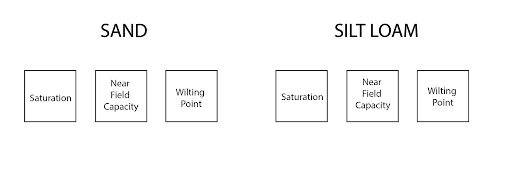
\includegraphics{soil-water-sand-siltloam-Picture1.png}

}

\caption{\label{fig-soilwater}Water Treatments}

\end{figure}

Using a moisture meter, you will construct a water retention curve for
each of these soils. You will use the moisture meter to measure the
volumetric water content and the tensiometer to measure the matric
potential in bars.

\textbf{NOTE: WATCH VIDEO TUTORIAL ON IPADS!! If you have any questions,
please ask the TA for assistance.}

Fill out the following table:

 
  \providecommand{\huxb}[2]{\arrayrulecolor[RGB]{#1}\global\arrayrulewidth=#2pt}
  \providecommand{\huxvb}[2]{\color[RGB]{#1}\vrule width #2pt}
  \providecommand{\huxtpad}[1]{\rule{0pt}{#1}}
  \providecommand{\huxbpad}[1]{\rule[-#1]{0pt}{#1}}

\begin{table}[h!]
\begin{centerbox}
\begin{threeparttable}
 
\setlength{\tabcolsep}{0pt}
\begin{tabularx}{0.9\textwidth}{p{0.3\textwidth} p{0.3\textwidth} p{0.3\textwidth}}


\hhline{>{\huxb{0, 0, 0}{1}}->{\huxb{0, 0, 0}{1}}->{\huxb{0, 0, 0}{1}}-}
\arrayrulecolor{black}

\multicolumn{1}{!{\huxvb{0, 0, 0}{1}}m{0.3\textwidth}!{\huxvb{0, 0, 0}{1}}}{\hspace{0pt}\parbox[c]{0.3\textwidth-0pt-4pt}{\huxtpad{0pt + 1em}\centering \textbf{}\huxbpad{4pt}}} &
\multicolumn{1}{m{0.3\textwidth}!{\huxvb{0, 0, 0}{1}}}{\hspace{4pt}\parbox[c]{0.3\textwidth-4pt-4pt}{\huxtpad{0pt + 1em}\centering \textbf{Matric Potential (Bars)}\huxbpad{4pt}}} &
\multicolumn{1}{m{0.3\textwidth}!{\huxvb{0, 0, 0}{1}}}{\hspace{4pt}\parbox[c]{0.3\textwidth-4pt-0pt}{\huxtpad{0pt + 1em}\centering \textbf{Volumetric H2O Content (θv)}\huxbpad{4pt}}} \tabularnewline[-0.5pt]


\hhline{>{\huxb{0, 0, 0}{1}}->{\huxb{0, 0, 0}{1}}->{\huxb{0, 0, 0}{1}}-}
\arrayrulecolor{black}

\multicolumn{1}{!{\huxvb{0, 0, 0}{1}}m{0.3\textwidth}!{\huxvb{0, 0, 0}{1}}}{\hspace{0pt}\parbox[c]{0.3\textwidth-0pt-4pt}{\huxtpad{4pt + 1em}\centering Sand (@ Saturation)\huxbpad{4pt}}} &
\multicolumn{1}{m{0.3\textwidth}!{\huxvb{0, 0, 0}{1}}}{\hspace{4pt}\parbox[c]{0.3\textwidth-4pt-4pt}{\huxtpad{4pt + 1em}\centering 0\huxbpad{4pt}}} &
\multicolumn{1}{m{0.3\textwidth}!{\huxvb{0, 0, 0}{1}}}{\hspace{4pt}\parbox[c]{0.3\textwidth-4pt-0pt}{\huxtpad{4pt + 1em}\centering \huxbpad{4pt}}} \tabularnewline[-0.5pt]


\hhline{>{\huxb{0, 0, 0}{1}}->{\huxb{0, 0, 0}{1}}->{\huxb{0, 0, 0}{1}}-}
\arrayrulecolor{black}

\multicolumn{1}{!{\huxvb{0, 0, 0}{1}}m{0.3\textwidth}!{\huxvb{0, 0, 0}{1}}}{\hspace{0pt}\parbox[c]{0.3\textwidth-0pt-4pt}{\huxtpad{4pt + 1em}\centering Sand (\~{}FC))\huxbpad{4pt}}} &
\multicolumn{1}{m{0.3\textwidth}!{\huxvb{0, 0, 0}{1}}}{\hspace{4pt}\parbox[c]{0.3\textwidth-4pt-4pt}{\huxtpad{4pt + 1em}\centering \huxbpad{4pt}}} &
\multicolumn{1}{m{0.3\textwidth}!{\huxvb{0, 0, 0}{1}}}{\hspace{4pt}\parbox[c]{0.3\textwidth-4pt-0pt}{\huxtpad{4pt + 1em}\centering \huxbpad{4pt}}} \tabularnewline[-0.5pt]


\hhline{>{\huxb{0, 0, 0}{1}}->{\huxb{0, 0, 0}{1}}->{\huxb{0, 0, 0}{1}}-}
\arrayrulecolor{black}

\multicolumn{1}{!{\huxvb{0, 0, 0}{1}}m{0.3\textwidth}!{\huxvb{0, 0, 0}{1}}}{\hspace{0pt}\parbox[c]{0.3\textwidth-0pt-4pt}{\huxtpad{4pt + 1em}\centering Sand (@ WP)\huxbpad{4pt}}} &
\multicolumn{1}{m{0.3\textwidth}!{\huxvb{0, 0, 0}{1}}}{\hspace{4pt}\parbox[c]{0.3\textwidth-4pt-4pt}{\huxtpad{4pt + 1em}\centering -15\huxbpad{4pt}}} &
\multicolumn{1}{m{0.3\textwidth}!{\huxvb{0, 0, 0}{1}}}{\hspace{4pt}\parbox[c]{0.3\textwidth-4pt-0pt}{\huxtpad{4pt + 1em}\centering \huxbpad{4pt}}} \tabularnewline[-0.5pt]


\hhline{>{\huxb{0, 0, 0}{1}}->{\huxb{0, 0, 0}{1}}->{\huxb{0, 0, 0}{1}}-}
\arrayrulecolor{black}

\multicolumn{1}{!{\huxvb{0, 0, 0}{1}}m{0.3\textwidth}!{\huxvb{0, 0, 0}{1}}}{\hspace{0pt}\parbox[c]{0.3\textwidth-0pt-4pt}{\huxtpad{4pt + 1em}\centering Silt Loam (@ Saturation)\huxbpad{4pt}}} &
\multicolumn{1}{m{0.3\textwidth}!{\huxvb{0, 0, 0}{1}}}{\hspace{4pt}\parbox[c]{0.3\textwidth-4pt-4pt}{\huxtpad{4pt + 1em}\centering 0\huxbpad{4pt}}} &
\multicolumn{1}{m{0.3\textwidth}!{\huxvb{0, 0, 0}{1}}}{\hspace{4pt}\parbox[c]{0.3\textwidth-4pt-0pt}{\huxtpad{4pt + 1em}\centering \huxbpad{4pt}}} \tabularnewline[-0.5pt]


\hhline{>{\huxb{0, 0, 0}{1}}->{\huxb{0, 0, 0}{1}}->{\huxb{0, 0, 0}{1}}-}
\arrayrulecolor{black}

\multicolumn{1}{!{\huxvb{0, 0, 0}{1}}m{0.3\textwidth}!{\huxvb{0, 0, 0}{1}}}{\hspace{0pt}\parbox[c]{0.3\textwidth-0pt-4pt}{\huxtpad{4pt + 1em}\centering Silt Loam (\~{}FC)\huxbpad{4pt}}} &
\multicolumn{1}{m{0.3\textwidth}!{\huxvb{0, 0, 0}{1}}}{\hspace{4pt}\parbox[c]{0.3\textwidth-4pt-4pt}{\huxtpad{4pt + 1em}\centering \huxbpad{4pt}}} &
\multicolumn{1}{m{0.3\textwidth}!{\huxvb{0, 0, 0}{1}}}{\hspace{4pt}\parbox[c]{0.3\textwidth-4pt-0pt}{\huxtpad{4pt + 1em}\centering \huxbpad{4pt}}} \tabularnewline[-0.5pt]


\hhline{>{\huxb{0, 0, 0}{1}}->{\huxb{0, 0, 0}{1}}->{\huxb{0, 0, 0}{1}}-}
\arrayrulecolor{black}

\multicolumn{1}{!{\huxvb{0, 0, 0}{1}}m{0.3\textwidth}!{\huxvb{0, 0, 0}{1}}}{\hspace{0pt}\parbox[c]{0.3\textwidth-0pt-4pt}{\huxtpad{4pt + 1em}\centering Silt Loam (@ WP)\huxbpad{0pt}}} &
\multicolumn{1}{m{0.3\textwidth}!{\huxvb{0, 0, 0}{1}}}{\hspace{4pt}\parbox[c]{0.3\textwidth-4pt-4pt}{\huxtpad{4pt + 1em}\centering -15\huxbpad{0pt}}} &
\multicolumn{1}{m{0.3\textwidth}!{\huxvb{0, 0, 0}{1}}}{\hspace{4pt}\parbox[c]{0.3\textwidth-4pt-0pt}{\huxtpad{4pt + 1em}\centering \huxbpad{0pt}}} \tabularnewline[-0.5pt]


\hhline{>{\huxb{0, 0, 0}{1}}->{\huxb{0, 0, 0}{1}}->{\huxb{0, 0, 0}{1}}-}
\arrayrulecolor{black}
\end{tabularx}
\end{threeparttable}\par\end{centerbox}

\end{table}
 

Use the data from the table on the previous page to construct water
retention curves (volumetric water content vs.~matric potential (i.e.,
tension, or negative pressure) note that the scale is logarithmic) for
each of these soils on the table below and answer the following
questions:

\begin{figure}

{\centering 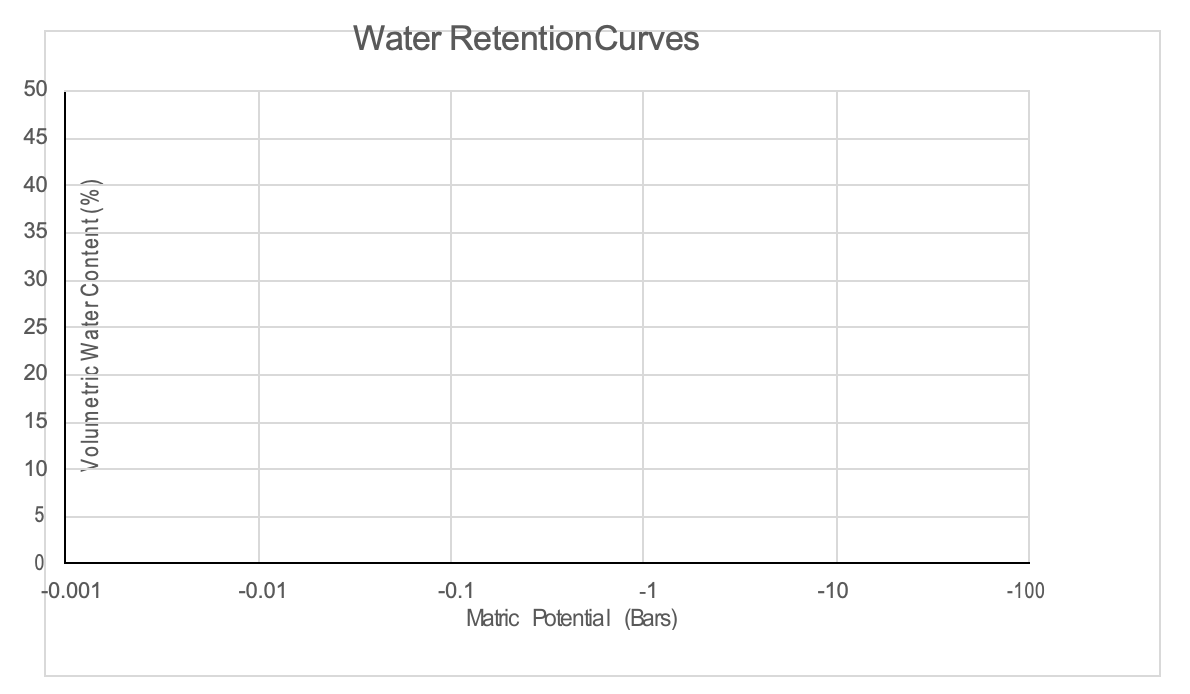
\includegraphics{water-retention-curve-Picture1.png}

}

\caption{\label{fig-waterretention}Water Retention Curve}

\end{figure}

\begin{enumerate}
\def\labelenumi{\arabic{enumi}.}
\tightlist
\item
  Using the graph above, estimate the total plant available water (in \%
  by volume) for each of these soils. FC is defined as -0.33 bars and
  wilting point is defined as -15 bars.
\end{enumerate}

~ ~ ~ ~

\begin{enumerate}
\def\labelenumi{\arabic{enumi}.}
\setcounter{enumi}{1}
\tightlist
\item
  Which soil will hold more plant available water when at field
  capacity? WHY?
\end{enumerate}

~ ~ ~ ~

\begin{enumerate}
\def\labelenumi{\arabic{enumi}.}
\setcounter{enumi}{2}
\tightlist
\item
  Describe the plant responses to these different treatments (i.e.~field
  capacity and wilting point).
\end{enumerate}

~ ~ ~ ~

\begin{enumerate}
\def\labelenumi{\arabic{enumi}.}
\setcounter{enumi}{3}
\tightlist
\item
  Using what you know about soil at this point in the class, describe
  the processes that are driving the plant response in each treatment.
  For example, think about why the saturated treatment looks the way it
  does? Why does the wilting point treatment look the way it does?
\end{enumerate}

~ ~ ~ ~

\hypertarget{investigation-b-determining-field-capacity}{%
\section{INVESTIGATION B: Determining Field
Capacity}\label{investigation-b-determining-field-capacity}}

\textbf{Preparation}

\begin{enumerate}
\def\labelenumi{\arabic{enumi}.}
\tightlist
\item
  Weigh a small plastic tray on the balance.
\item
  Move the weight on the far beam to 20 grams
\item
  With a spoon, add soil to the tray until balanced
\item
  Take a single sheet of the round filter paper and fold it in half and
  then fold it in half again. You should be able to create a small cone
  of filter paper that will fit inside one of the funnels.
\item
  Once you have the filter in place in the funnel, add 20 grams of soil
  to the funnel
\item
  Carefully fill one of the graduated cylinders (BLUE base) with 25 ml
  of water
\item
  Place the funnel with the filter paper and soil on top of one of the
  100 ml graduated cylinder.
\item
  Carefully pour all 25 ml of water on top of the soil. Add about a
  third of the water, wait for it to be absorbed into the soil. Then
  slowly add the remainder. Do not add so much water at one time that it
  overtops the filter paper. \emph{The silt loam may take 10 minutes or
  so to add all of the water.}
\item
  Record the amount of water (in ml) that has passed through the soil
  sample and has collected in the graduated clynder. Assume 2ml of water
  is absorbed by the filter paper.
\end{enumerate}

Repeat this process for the soils labeled Sand and Silt Loam and record
your results in the table below.

\textbf{Volume retained in the soil} = (25mL) - (Volume retained on
filter paper) - (Volume passed through the soil).

This is an estimate of field capacity.

\textbf{θg at Field Capacity} = (mL H2O retained) / (g dry soil),
because 1 mL H2O = 1 g H2O.

Assume your 20 g of soil was oven dry.

 
  \providecommand{\huxb}[2]{\arrayrulecolor[RGB]{#1}\global\arrayrulewidth=#2pt}
  \providecommand{\huxvb}[2]{\color[RGB]{#1}\vrule width #2pt}
  \providecommand{\huxtpad}[1]{\rule{0pt}{#1}}
  \providecommand{\huxbpad}[1]{\rule[-#1]{0pt}{#1}}

\begin{table}[h!]
\begin{centerbox}
\begin{threeparttable}
 
\setlength{\tabcolsep}{0pt}
\begin{tabularx}{0.9\textwidth}{p{0.18\textwidth} p{0.18\textwidth} p{0.18\textwidth} p{0.18\textwidth} p{0.18\textwidth}}


\hhline{>{\huxb{0, 0, 0}{1}}->{\huxb{0, 0, 0}{1}}->{\huxb{0, 0, 0}{1}}->{\huxb{0, 0, 0}{1}}->{\huxb{0, 0, 0}{1}}-}
\arrayrulecolor{black}

\multicolumn{1}{!{\huxvb{0, 0, 0}{1}}m{0.18\textwidth}!{\huxvb{0, 0, 0}{1}}}{\hspace{0pt}\parbox[c]{0.18\textwidth-0pt-4pt}{\huxtpad{0pt + 1em}\centering \textbf{}\huxbpad{4pt}}} &
\multicolumn{1}{m{0.18\textwidth}!{\huxvb{0, 0, 0}{1}}}{\hspace{4pt}\parbox[c]{0.18\textwidth-4pt-4pt}{\huxtpad{0pt + 1em}\centering \textbf{Volume Retained on the Filter Paper}\huxbpad{4pt}}} &
\multicolumn{1}{m{0.18\textwidth}!{\huxvb{0, 0, 0}{1}}}{\hspace{4pt}\parbox[c]{0.18\textwidth-4pt-4pt}{\huxtpad{0pt + 1em}\centering \textbf{Volume Passed Through the Soil}\huxbpad{4pt}}} &
\multicolumn{1}{m{0.18\textwidth}!{\huxvb{0, 0, 0}{1}}}{\hspace{4pt}\parbox[c]{0.18\textwidth-4pt-4pt}{\huxtpad{0pt + 1em}\centering \textbf{Volume Retained in the Soil}\huxbpad{4pt}}} &
\multicolumn{1}{m{0.18\textwidth}!{\huxvb{0, 0, 0}{1}}}{\hspace{4pt}\parbox[c]{0.18\textwidth-4pt-0pt}{\huxtpad{0pt + 1em}\centering \textbf{Calculate θg at Field Capacity}\huxbpad{4pt}}} \tabularnewline[-0.5pt]


\hhline{>{\huxb{0, 0, 0}{1}}->{\huxb{0, 0, 0}{1}}->{\huxb{0, 0, 0}{1}}->{\huxb{0, 0, 0}{1}}->{\huxb{0, 0, 0}{1}}-}
\arrayrulecolor{black}

\multicolumn{1}{!{\huxvb{0, 0, 0}{1}}m{0.18\textwidth}!{\huxvb{0, 0, 0}{1}}}{\hspace{0pt}\parbox[c]{0.18\textwidth-0pt-4pt}{\huxtpad{4pt + 1em}\centering Sand\huxbpad{4pt}}} &
\multicolumn{1}{m{0.18\textwidth}!{\huxvb{0, 0, 0}{1}}}{\hspace{4pt}\parbox[c]{0.18\textwidth-4pt-4pt}{\huxtpad{4pt + 1em}\centering 2 mL\huxbpad{4pt}}} &
\multicolumn{1}{m{0.18\textwidth}!{\huxvb{0, 0, 0}{1}}}{\hspace{4pt}\parbox[c]{0.18\textwidth-4pt-4pt}{\huxtpad{4pt + 1em}\centering \huxbpad{4pt}}} &
\multicolumn{1}{m{0.18\textwidth}!{\huxvb{0, 0, 0}{1}}}{\hspace{4pt}\parbox[c]{0.18\textwidth-4pt-4pt}{\huxtpad{4pt + 1em}\centering \huxbpad{4pt}}} &
\multicolumn{1}{m{0.18\textwidth}!{\huxvb{0, 0, 0}{1}}}{\hspace{4pt}\parbox[c]{0.18\textwidth-4pt-0pt}{\huxtpad{4pt + 1em}\centering \huxbpad{4pt}}} \tabularnewline[-0.5pt]


\hhline{>{\huxb{0, 0, 0}{1}}->{\huxb{0, 0, 0}{1}}->{\huxb{0, 0, 0}{1}}->{\huxb{0, 0, 0}{1}}->{\huxb{0, 0, 0}{1}}-}
\arrayrulecolor{black}

\multicolumn{1}{!{\huxvb{0, 0, 0}{1}}m{0.18\textwidth}!{\huxvb{0, 0, 0}{1}}}{\hspace{0pt}\parbox[c]{0.18\textwidth-0pt-4pt}{\huxtpad{4pt + 1em}\centering Silt Loam\huxbpad{0pt}}} &
\multicolumn{1}{m{0.18\textwidth}!{\huxvb{0, 0, 0}{1}}}{\hspace{4pt}\parbox[c]{0.18\textwidth-4pt-4pt}{\huxtpad{4pt + 1em}\centering 2 mL\huxbpad{0pt}}} &
\multicolumn{1}{m{0.18\textwidth}!{\huxvb{0, 0, 0}{1}}}{\hspace{4pt}\parbox[c]{0.18\textwidth-4pt-4pt}{\huxtpad{4pt + 1em}\centering \huxbpad{0pt}}} &
\multicolumn{1}{m{0.18\textwidth}!{\huxvb{0, 0, 0}{1}}}{\hspace{4pt}\parbox[c]{0.18\textwidth-4pt-4pt}{\huxtpad{4pt + 1em}\centering \huxbpad{0pt}}} &
\multicolumn{1}{m{0.18\textwidth}!{\huxvb{0, 0, 0}{1}}}{\hspace{4pt}\parbox[c]{0.18\textwidth-4pt-0pt}{\huxtpad{4pt + 1em}\centering \huxbpad{0pt}}} \tabularnewline[-0.5pt]


\hhline{>{\huxb{0, 0, 0}{1}}->{\huxb{0, 0, 0}{1}}->{\huxb{0, 0, 0}{1}}->{\huxb{0, 0, 0}{1}}->{\huxb{0, 0, 0}{1}}-}
\arrayrulecolor{black}
\end{tabularx}
\end{threeparttable}\par\end{centerbox}

\end{table}
 

\begin{enumerate}
\def\labelenumi{\arabic{enumi}.}
\tightlist
\item
  Explain why the different soil textures retained differing amounts of
  water.
\end{enumerate}

~ ~ ~ ~

\begin{enumerate}
\def\labelenumi{\arabic{enumi}.}
\setcounter{enumi}{1}
\tightlist
\item
  Which of these textures has the highest water content at field
  capacity?
\end{enumerate}

~ ~ ~ ~

\hypertarget{investigation-c-tensiometer-observation}{%
\section{INVESTIGATION C: Tensiometer
Observation}\label{investigation-c-tensiometer-observation}}

In this investigation you can observe the use of a tensiometer to
measure matric potential (the tension at which water is pulled by the
soil) for two different soils at different water contents. The
tensiometer is essentially a water column with a porous ceramic tip at
the bottom. The pores in the ceramic are so small that water will not
move through the ceramic under the influence of gravity alone (i.e.~the
force of gravity does not pull down hard enough for the water to move
through). However, you now know that due to adhesion, cohesion and
capillary action that soils can exert a tension on water and pull it
against gravity. The vacuum gauge readings show the relative amount of
tension that the soil is exerting on the water. To make the gauges
reasonable for the general public to use, scales are usually from 0-100
in positive numbers -- a high reading on the gauge is caused by a dry
soil that has a high tension. Note that this is different than what we
discussed in lecture in that the values are positive rather than
negative -- these are designed for consumer use and are scaled and
calibrated based on convenient numbers, not fundamental principles, but
the concepts are exactly the same. These types of tensiometers are
commonly used for irrigation scheduling to let the land managers know
when to turn on the sprinklers; at a golf course for example.

Read the tension gauge (the units are in centibars of tension (if you
put a negative in front of the number and divide by 100, you would have
``bars'' of tension as we discussed in class)) and note how it has
changed since the start of the week for each soil. Mark the current
gauge reading and time on the graph so we can chart the changes
throughout the week.

\textbf{Tensiometer Readings:}

Loamy Sand:
\_\_\_\_\_\_\_\_\_\_\_\_\_~~~~~~~~~~~~~~~~~~~~~~~~~~~~~~~~Silt Loam:
\_\_\_\_\_\_\_\_\_\_\_\_\_

\hypertarget{investigation-d-observations-of-capillary-action}{%
\section{INVESTIGATION D: Observations of Capillary
Action}\label{investigation-d-observations-of-capillary-action}}

Capillary action enables soil moisture to move in any direction within
the soil as water moves from wetter areas to drier areas. Observe the
different sized capillary tubes and the height at which the water
reaches in each tube.

\begin{enumerate}
\def\labelenumi{\arabic{enumi}.}
\tightlist
\item
  Explain the relationship between the height of the water in the
  capillary tubes and the tube diameter using the terms adhesion,
  cohesion and gravity.
\end{enumerate}

~ ~ ~ ~ ~ ~ ~ ~ ~ ~

\begin{enumerate}
\def\labelenumi{\arabic{enumi}.}
\setcounter{enumi}{1}
\tightlist
\item
  Now observe the two soil columns -- one is fine sand (particles
  \textasciitilde{} 200um in diameter) and the other a coarse sand
  (particles \textasciitilde{} 750um in diameter) and observe the height
  of water rise in each column. Explain the differences in the height of
  rise based on what you know about soil textural class, particle size,
  and pore size.
\end{enumerate}

~ ~ ~ ~ ~ ~ ~ ~ ~ ~

\begin{enumerate}
\def\labelenumi{\arabic{enumi}.}
\setcounter{enumi}{2}
\tightlist
\item
  The zone between the totally saturated soil material below the water
  surface in the tub and the highest height of rise due to matric
  potential is sometimes called the ``capillary fringe'' -- it
  represents the height at which water has been pulled up from a
  saturated zone against gravity by capillary action or matric
  potential. Would you expect a silty clay or a sandy clay loam to have
  a larger capillary fringe (you might want to reference your textural
  triangle)? Why?
\end{enumerate}

~ ~ ~ ~ ~ ~ ~ ~ ~ ~

\hypertarget{investigation-e-determining-soil-moisture-by-weight-and-volume}{%
\section{INVESTIGATION E: Determining Soil Moisture by Weight and
Volume}\label{investigation-e-determining-soil-moisture-by-weight-and-volume}}

The soil can that you prepared last week (present soil condition) has
been oven dried. Weigh the oven dry soil along with the can and lid.

Using the data you recorded last week, fill in the table below:

 
  \providecommand{\huxb}[2]{\arrayrulecolor[RGB]{#1}\global\arrayrulewidth=#2pt}
  \providecommand{\huxvb}[2]{\color[RGB]{#1}\vrule width #2pt}
  \providecommand{\huxtpad}[1]{\rule{0pt}{#1}}
  \providecommand{\huxbpad}[1]{\rule[-#1]{0pt}{#1}}

\begin{table}[h!]
\begin{centerbox}
\begin{threeparttable}
 
\setlength{\tabcolsep}{0pt}
\begin{tabularx}{0.9\textwidth}{p{0.45\textwidth} p{0.45\textwidth}}


\hhline{>{\huxb{0, 0, 0}{1}}->{\huxb{0, 0, 0}{1}}-}
\arrayrulecolor{black}

\multicolumn{1}{!{\huxvb{0, 0, 0}{1}}m{0.45\textwidth}!{\huxvb{0, 0, 0}{1}}}{\hspace{0pt}\parbox[c]{0.45\textwidth-0pt-4pt}{\huxtpad{0pt + 1em}\centering \textbf{Property}\huxbpad{4pt}}} &
\multicolumn{1}{m{0.45\textwidth}!{\huxvb{0, 0, 0}{1}}}{\hspace{4pt}\parbox[c]{0.45\textwidth-4pt-0pt}{\huxtpad{0pt + 1em}\raggedleft \textbf{Measurement}\huxbpad{4pt}}} \tabularnewline[-0.5pt]


\hhline{>{\huxb{0, 0, 0}{1}}->{\huxb{0, 0, 0}{1}}-}
\arrayrulecolor{black}

\multicolumn{1}{!{\huxvb{0, 0, 0}{1}}m{0.45\textwidth}!{\huxvb{0, 0, 0}{1}}}{\hspace{0pt}\parbox[c]{0.45\textwidth-0pt-4pt}{\huxtpad{4pt + 1em}\centering Weight of can\huxbpad{4pt}}} &
\multicolumn{1}{m{0.45\textwidth}!{\huxvb{0, 0, 0}{1}}}{\hspace{4pt}\parbox[c]{0.45\textwidth-4pt-0pt}{\huxtpad{4pt + 1em}\raggedleft grams\huxbpad{4pt}}} \tabularnewline[-0.5pt]


\hhline{>{\huxb{0, 0, 0}{1}}->{\huxb{0, 0, 0}{1}}-}
\arrayrulecolor{black}

\multicolumn{1}{!{\huxvb{0, 0, 0}{1}}m{0.45\textwidth}!{\huxvb{0, 0, 0}{1}}}{\hspace{0pt}\parbox[c]{0.45\textwidth-0pt-4pt}{\huxtpad{4pt + 1em}\centering Weight of moist soil + can\huxbpad{4pt}}} &
\multicolumn{1}{m{0.45\textwidth}!{\huxvb{0, 0, 0}{1}}}{\hspace{4pt}\parbox[c]{0.45\textwidth-4pt-0pt}{\huxtpad{4pt + 1em}\raggedleft grams\huxbpad{4pt}}} \tabularnewline[-0.5pt]


\hhline{>{\huxb{0, 0, 0}{1}}->{\huxb{0, 0, 0}{1}}-}
\arrayrulecolor{black}

\multicolumn{1}{!{\huxvb{0, 0, 0}{1}}m{0.45\textwidth}!{\huxvb{0, 0, 0}{1}}}{\hspace{0pt}\parbox[c]{0.45\textwidth-0pt-4pt}{\huxtpad{4pt + 1em}\centering Weight of moist soil\huxbpad{4pt}}} &
\multicolumn{1}{m{0.45\textwidth}!{\huxvb{0, 0, 0}{1}}}{\hspace{4pt}\parbox[c]{0.45\textwidth-4pt-0pt}{\huxtpad{4pt + 1em}\raggedleft grams\huxbpad{4pt}}} \tabularnewline[-0.5pt]


\hhline{>{\huxb{0, 0, 0}{1}}->{\huxb{0, 0, 0}{1}}-}
\arrayrulecolor{black}

\multicolumn{1}{!{\huxvb{0, 0, 0}{1}}m{0.45\textwidth}!{\huxvb{0, 0, 0}{1}}}{\hspace{0pt}\parbox[c]{0.45\textwidth-0pt-4pt}{\huxtpad{4pt + 1em}\centering Weight of oven dry soil + can\huxbpad{4pt}}} &
\multicolumn{1}{m{0.45\textwidth}!{\huxvb{0, 0, 0}{1}}}{\hspace{4pt}\parbox[c]{0.45\textwidth-4pt-0pt}{\huxtpad{4pt + 1em}\raggedleft grams\huxbpad{4pt}}} \tabularnewline[-0.5pt]


\hhline{>{\huxb{0, 0, 0}{1}}->{\huxb{0, 0, 0}{1}}-}
\arrayrulecolor{black}

\multicolumn{1}{!{\huxvb{0, 0, 0}{1}}m{0.45\textwidth}!{\huxvb{0, 0, 0}{1}}}{\hspace{0pt}\parbox[c]{0.45\textwidth-0pt-4pt}{\huxtpad{4pt + 1em}\centering Weight of oven-dried soil\huxbpad{4pt}}} &
\multicolumn{1}{m{0.45\textwidth}!{\huxvb{0, 0, 0}{1}}}{\hspace{4pt}\parbox[c]{0.45\textwidth-4pt-0pt}{\huxtpad{4pt + 1em}\raggedleft grams\huxbpad{4pt}}} \tabularnewline[-0.5pt]


\hhline{>{\huxb{0, 0, 0}{1}}->{\huxb{0, 0, 0}{1}}-}
\arrayrulecolor{black}

\multicolumn{1}{!{\huxvb{0, 0, 0}{1}}m{0.45\textwidth}!{\huxvb{0, 0, 0}{1}}}{\hspace{0pt}\parbox[c]{0.45\textwidth-0pt-4pt}{\huxtpad{4pt + 1em}\centering θg of moist soil last week\huxbpad{0pt}}} &
\multicolumn{1}{m{0.45\textwidth}!{\huxvb{0, 0, 0}{1}}}{\hspace{4pt}\parbox[c]{0.45\textwidth-4pt-0pt}{\huxtpad{4pt + 1em}\raggedleft \%\huxbpad{0pt}}} \tabularnewline[-0.5pt]


\hhline{>{\huxb{0, 0, 0}{1}}->{\huxb{0, 0, 0}{1}}-}
\arrayrulecolor{black}
\end{tabularx}
\end{threeparttable}\par\end{centerbox}

\end{table}
 

The bulk density of the moist soil in the bucket last week was 1.3
g/cm3. Calculate the volumetric water content (θv):

\hypertarget{investigation-f-soil-water-problems}{%
\section{INVESTIGATION F: Soil Water
Problems}\label{investigation-f-soil-water-problems}}

You need to know how to calculate the amount of water in a soil at
various water potentials. This knowledge will help you understand that
it is not the total amount of water in a soil that determines whether
water is available to plants but it is the plant available water (PAW)
that matters.

Given:

Soil Core Volume = \textbf{250 cm3} (for each soil core below)

Weight of soil core at -0.33 bar (field capacity: FC) = \textbf{420 g}

Weight of soil core at -15 bar (wilting point: WP) = \textbf{350 g}

Weight of soil core at present sampling time = \textbf{395 g}

Weight of Oven dry soil core = \textbf{300 g}

\begin{enumerate}
\def\labelenumi{\arabic{enumi}.}
\tightlist
\item
  What is the bulk density?
\end{enumerate}

~ ~ ~

\begin{enumerate}
\def\labelenumi{\arabic{enumi}.}
\setcounter{enumi}{1}
\tightlist
\item
  What is \textbf{θg(FC)}? ~~~~~~~~~~~~~~~~~~~~~~~~What is
  \textbf{θg(WP)}? ~~~~~~~~~~~~~~~~~~~~~~~~What is \textbf{θg(at
  present)}?
\end{enumerate}

\begin{enumerate}
\def\labelenumi{\arabic{enumi}.}
\setcounter{enumi}{2}
\tightlist
\item
  What is \textbf{θv(FC)}? ~~~~~~~~~~~~~~~~~~~~~~~~What is
  \textbf{θv(WP)}? ~~~~~~~~~~~~~~~~~~~~~~~~What is \textbf{θv(at
  present)}?
\end{enumerate}

\begin{enumerate}
\def\labelenumi{\arabic{enumi}.}
\setcounter{enumi}{3}
\tightlist
\item
  What is the total possible plant available water by volume? Remember,
  total possible plant available water (PAW) for a given soil texture is
  the difference between the volumetric water content at field capacity
  (FC) and the wilting point (WP): \textbf{θv(FC) -- θv(WP)}?
\end{enumerate}

\begin{enumerate}
\def\labelenumi{\arabic{enumi}.}
\setcounter{enumi}{4}
\tightlist
\item
  How many \emph{inches} of plant available water would there be at
  field capacity if the soil layer was 3 ft. thick?
\end{enumerate}

\begin{enumerate}
\def\labelenumi{\arabic{enumi}.}
\setcounter{enumi}{5}
\tightlist
\item
  How many inches of plant available water are left in the 3 ft. soil
  layer in the present condition \emph{(i.e.~at the time of sampling in
  the field)}?
\end{enumerate}

\begin{enumerate}
\def\labelenumi{\arabic{enumi}.}
\setcounter{enumi}{6}
\tightlist
\item
  If a corn crop requires \textasciitilde{} 0.3 inches of water per day
  during the height of the growing season and the roots have access to
  the entire 3 ft layer you used for calculations in 5 and 6, how many
  days of corn growth can the current soil moisture storage support
  (without additional rainfall or irrigation) before the corn begins to
  wilt?
\end{enumerate}

\bookmarksetup{startatroot}

\hypertarget{biological-processes-1}{%
\chapter{\texorpdfstring{\textbf{Biological Processes
(1)}}{Biological Processes (1)}}\label{biological-processes-1}}

\begin{tcolorbox}[enhanced jigsaw, colframe=quarto-callout-note-color-frame, coltitle=black, arc=.35mm, breakable, bottomrule=.15mm, colback=white, rightrule=.15mm, toprule=.15mm, opacityback=0, bottomtitle=1mm, left=2mm, titlerule=0mm, leftrule=.75mm, opacitybacktitle=0.6, toptitle=1mm, title=\textcolor{quarto-callout-note-color}{\faInfo}\hspace{0.5em}{Objectives}, colbacktitle=quarto-callout-note-color!10!white]

\begin{itemize}
\tightlist
\item
  Understand the dynamics of the nitrogen cycle.
\item
  Observe nodules involved in symbiotic N2 fixation.
\item
  Understand the effect of biological activity and soil organic matter
  on aggregate stability.
\item
  Observe soil fauna.
\item
  Inoculate plates.
\end{itemize}

\end{tcolorbox}

\begin{tcolorbox}[enhanced jigsaw, colframe=quarto-callout-tip-color-frame, coltitle=black, arc=.35mm, breakable, bottomrule=.15mm, colback=white, rightrule=.15mm, toprule=.15mm, opacityback=0, bottomtitle=1mm, left=2mm, titlerule=0mm, leftrule=.75mm, opacitybacktitle=0.6, toptitle=1mm, title=\textcolor{quarto-callout-tip-color}{\faLightbulb}\hspace{0.5em}{Key Words \& Concepts}, colbacktitle=quarto-callout-tip-color!10!white]

\begin{itemize}
\tightlist
\item
  Leaching
\item
  Nitrification
\item
  Mineralization
\item
  Denitrification
\item
  Volatilization
\item
  Aggregates
\item
  Microbial Gums
\item
  Symbiotic Fixation
\item
  Nodules
\item
  \emph{Rhizobium}
\end{itemize}

\end{tcolorbox}

\hypertarget{investigation-a-forms-of-nitrogen}{%
\section{INVESTIGATION A: Forms of
Nitrogen}\label{investigation-a-forms-of-nitrogen}}

You will probably come across many complex and confusing representations
of the nitrogen cycle in other venues. Use your knowledge of the
simplified representation of the nitrogen cycle that we discussed in
class to fill in the blanks in the appropriate places on the diagram
below (which I note is also incomplete).

\begin{figure}

{\centering 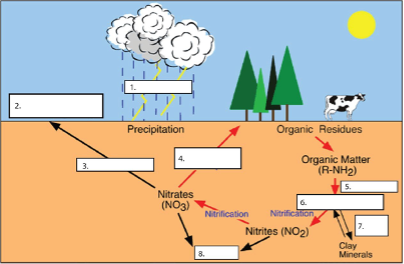
\includegraphics{forms-of-nitrogenPicture1.png}

}

\caption{\label{fig-nitrogen}The Nitrogen Cycle}

\end{figure}

 
  \providecommand{\huxb}[2]{\arrayrulecolor[RGB]{#1}\global\arrayrulewidth=#2pt}
  \providecommand{\huxvb}[2]{\color[RGB]{#1}\vrule width #2pt}
  \providecommand{\huxtpad}[1]{\rule{0pt}{#1}}
  \providecommand{\huxbpad}[1]{\rule[-#1]{0pt}{#1}}

\begin{table}[h!]
\begin{centerbox}
\begin{threeparttable}
 
\setlength{\tabcolsep}{0pt}
\begin{tabularx}{0.9\textwidth}{p{0.45\textwidth} p{0.45\textwidth}}


\hhline{>{\huxb{0, 0, 0}{1}}->{\huxb{0, 0, 0}{1}}-}
\arrayrulecolor{black}

\multicolumn{1}{!{\huxvb{0, 0, 0}{1}}m{0.45\textwidth}!{\huxvb{0, 0, 0}{1}}}{\hspace{0pt}\parbox[c]{0.45\textwidth-0pt-4pt}{\huxtpad{0pt + 1em}\raggedright \textbf{Fill in Each Number with Best Choice from Word Bank}\huxbpad{4pt}}} &
\multicolumn{1}{m{0.45\textwidth}!{\huxvb{0, 0, 0}{1}}}{\hspace{4pt}\parbox[c]{0.45\textwidth-4pt-0pt}{\huxtpad{0pt + 1em}\centering \textbf{Word Bank}\huxbpad{4pt}}} \tabularnewline[-0.5pt]


\hhline{>{\huxb{0, 0, 0}{1}}->{\huxb{0, 0, 0}{1}}-}
\arrayrulecolor{black}

\multicolumn{1}{!{\huxvb{0, 0, 0}{1}}m{0.45\textwidth}!{\huxvb{0, 0, 0}{1}}}{\hspace{0pt}\parbox[c]{0.45\textwidth-0pt-4pt}{\huxtpad{4pt + 1em}\raggedright 1.\huxbpad{4pt}}} &
\multicolumn{1}{m{0.45\textwidth}!{\huxvb{0, 0, 0}{1}}}{\hspace{4pt}\parbox[c]{0.45\textwidth-4pt-0pt}{\huxtpad{4pt + 1em}\centering N2\huxbpad{4pt}}} \tabularnewline[-0.5pt]


\hhline{>{\huxb{0, 0, 0}{1}}->{\huxb{0, 0, 0}{1}}-}
\arrayrulecolor{black}

\multicolumn{1}{!{\huxvb{0, 0, 0}{1}}m{0.45\textwidth}!{\huxvb{0, 0, 0}{1}}}{\hspace{0pt}\parbox[c]{0.45\textwidth-0pt-4pt}{\huxtpad{4pt + 1em}\raggedright 2.\huxbpad{4pt}}} &
\multicolumn{1}{m{0.45\textwidth}!{\huxvb{0, 0, 0}{1}}}{\hspace{4pt}\parbox[c]{0.45\textwidth-4pt-0pt}{\huxtpad{4pt + 1em}\centering Abiotic N Fixation\huxbpad{4pt}}} \tabularnewline[-0.5pt]


\hhline{>{\huxb{0, 0, 0}{1}}->{\huxb{0, 0, 0}{1}}-}
\arrayrulecolor{black}

\multicolumn{1}{!{\huxvb{0, 0, 0}{1}}m{0.45\textwidth}!{\huxvb{0, 0, 0}{1}}}{\hspace{0pt}\parbox[c]{0.45\textwidth-0pt-4pt}{\huxtpad{4pt + 1em}\raggedright 3.\huxbpad{4pt}}} &
\multicolumn{1}{m{0.45\textwidth}!{\huxvb{0, 0, 0}{1}}}{\hspace{4pt}\parbox[c]{0.45\textwidth-4pt-0pt}{\huxtpad{4pt + 1em}\centering Cation Exchange\huxbpad{4pt}}} \tabularnewline[-0.5pt]


\hhline{>{\huxb{0, 0, 0}{1}}->{\huxb{0, 0, 0}{1}}-}
\arrayrulecolor{black}

\multicolumn{1}{!{\huxvb{0, 0, 0}{1}}m{0.45\textwidth}!{\huxvb{0, 0, 0}{1}}}{\hspace{0pt}\parbox[c]{0.45\textwidth-0pt-4pt}{\huxtpad{4pt + 1em}\raggedright 4.\huxbpad{4pt}}} &
\multicolumn{1}{m{0.45\textwidth}!{\huxvb{0, 0, 0}{1}}}{\hspace{4pt}\parbox[c]{0.45\textwidth-4pt-0pt}{\huxtpad{4pt + 1em}\centering NH4+\huxbpad{4pt}}} \tabularnewline[-0.5pt]


\hhline{>{\huxb{0, 0, 0}{1}}->{\huxb{0, 0, 0}{1}}-}
\arrayrulecolor{black}

\multicolumn{1}{!{\huxvb{0, 0, 0}{1}}m{0.45\textwidth}!{\huxvb{0, 0, 0}{1}}}{\hspace{0pt}\parbox[c]{0.45\textwidth-0pt-4pt}{\huxtpad{4pt + 1em}\raggedright 5.\huxbpad{4pt}}} &
\multicolumn{1}{m{0.45\textwidth}!{\huxvb{0, 0, 0}{1}}}{\hspace{4pt}\parbox[c]{0.45\textwidth-4pt-0pt}{\huxtpad{4pt + 1em}\centering Mineralization\huxbpad{4pt}}} \tabularnewline[-0.5pt]


\hhline{>{\huxb{0, 0, 0}{1}}->{\huxb{0, 0, 0}{1}}-}
\arrayrulecolor{black}

\multicolumn{1}{!{\huxvb{0, 0, 0}{1}}m{0.45\textwidth}!{\huxvb{0, 0, 0}{1}}}{\hspace{0pt}\parbox[c]{0.45\textwidth-0pt-4pt}{\huxtpad{4pt + 1em}\raggedright 6.\huxbpad{4pt}}} &
\multicolumn{1}{m{0.45\textwidth}!{\huxvb{0, 0, 0}{1}}}{\hspace{4pt}\parbox[c]{0.45\textwidth-4pt-0pt}{\huxtpad{4pt + 1em}\centering Plant Uptake\huxbpad{4pt}}} \tabularnewline[-0.5pt]


\hhline{>{\huxb{0, 0, 0}{1}}->{\huxb{0, 0, 0}{1}}-}
\arrayrulecolor{black}

\multicolumn{1}{!{\huxvb{0, 0, 0}{1}}m{0.45\textwidth}!{\huxvb{0, 0, 0}{1}}}{\hspace{0pt}\parbox[c]{0.45\textwidth-0pt-4pt}{\huxtpad{4pt + 1em}\raggedright 7.\huxbpad{4pt}}} &
\multicolumn{1}{m{0.45\textwidth}!{\huxvb{0, 0, 0}{1}}}{\hspace{4pt}\parbox[c]{0.45\textwidth-4pt-0pt}{\huxtpad{4pt + 1em}\centering Denitrification\huxbpad{4pt}}} \tabularnewline[-0.5pt]


\hhline{>{\huxb{0, 0, 0}{1}}->{\huxb{0, 0, 0}{1}}-}
\arrayrulecolor{black}

\multicolumn{1}{!{\huxvb{0, 0, 0}{1}}m{0.45\textwidth}!{\huxvb{0, 0, 0}{1}}}{\hspace{0pt}\parbox[c]{0.45\textwidth-0pt-4pt}{\huxtpad{4pt + 1em}\raggedright 8.\huxbpad{0pt}}} &
\multicolumn{1}{m{0.45\textwidth}!{\huxvb{0, 0, 0}{1}}}{\hspace{4pt}\parbox[c]{0.45\textwidth-4pt-0pt}{\huxtpad{4pt + 1em}\centering Leaching\huxbpad{0pt}}} \tabularnewline[-0.5pt]


\hhline{>{\huxb{0, 0, 0}{1}}->{\huxb{0, 0, 0}{1}}-}
\arrayrulecolor{black}
\end{tabularx}
\end{threeparttable}\par\end{centerbox}

\end{table}
 

\hypertarget{investigation-b1-observing-nodules}{%
\section{INVESTIGATION B1: Observing
Nodules}\label{investigation-b1-observing-nodules}}

Observe the roots of the live alfalfa and soybean plants (both
uninoculated (no nodules) and inoculated (nodules)) which have been
provided for you to look at. Don't be afraid to pull a plant out and
look at the roots! Put it in the container of soil when finished.
Rhizobia is the common name given to a group of small, rod- shaped, Gram
negative bacteria, which collectively have the ability to induce nodule
production on the roots of leguminous plants. Observe the nodules on the
plants in the jars.

Draw a diagram of a nodule and a root:

~ ~ ~ ~ ~

\hypertarget{investigation-b2-dissecting-nodules}{%
\section{INVESTIGATION B2: Dissecting
Nodules}\label{investigation-b2-dissecting-nodules}}

Pluck a nodule off of either a soybean or alfalfa root and cut it open
with a razor blade under the dissecting scopes. When you cut open an
active nitrogen-fixing nodule, a significant portion of the nodule
should be pink or red in color. This color is due to the presence of a
hemoglobin similar to that found in blood (known as ``leghemoglobin'' in
legumes), and regulates oxygen supply, in this case, to the bacteria.
The amount of hemoglobin present is usually closely correlated to amount
of nitrogen fixed, with white or green-colored nodules usually very
limited in their ability to fix nitrogen. Remember though that nodules
have a finite life span (in the case of soybean estimated at 50-60 days)
so that toward the end of the growing season many of the initial nodules
will have already begun to senesce, and are brown or green in color,
while the more active nitrogen-fixing nodules may now be located on
lateral roots (see \emph{Rhizobium} Research Laboratory at
www.rhizobium.umn.edu). Cut open a nodule from the samples provided,
view under the microscope, and complete the following table.

 
  \providecommand{\huxb}[2]{\arrayrulecolor[RGB]{#1}\global\arrayrulewidth=#2pt}
  \providecommand{\huxvb}[2]{\color[RGB]{#1}\vrule width #2pt}
  \providecommand{\huxtpad}[1]{\rule{0pt}{#1}}
  \providecommand{\huxbpad}[1]{\rule[-#1]{0pt}{#1}}

\begin{table}[h!]
\begin{centerbox}
\begin{threeparttable}
 
\setlength{\tabcolsep}{0pt}
\begin{tabularx}{0.9\textwidth}{p{0.45\textwidth} p{0.45\textwidth}}


\hhline{>{\huxb{0, 0, 0}{1}}->{\huxb{0, 0, 0}{1}}-}
\arrayrulecolor{black}

\multicolumn{1}{!{\huxvb{0, 0, 0}{1}}m{0.45\textwidth}!{\huxvb{0, 0, 0}{1}}}{\hspace{0pt}\parbox[c]{0.45\textwidth-0pt-4pt}{\huxtpad{0pt + 1em}\centering \textbf{Nodule Color}\huxbpad{4pt}}} &
\multicolumn{1}{m{0.45\textwidth}!{\huxvb{0, 0, 0}{1}}}{\hspace{4pt}\parbox[c]{0.45\textwidth-4pt-0pt}{\huxtpad{0pt + 1em}\centering \textbf{Explanation}\huxbpad{4pt}}} \tabularnewline[-0.5pt]


\hhline{>{\huxb{0, 0, 0}{1}}->{\huxb{0, 0, 0}{1}}-}
\arrayrulecolor{black}

\multicolumn{1}{!{\huxvb{0, 0, 0}{1}}m{0.45\textwidth}!{\huxvb{0, 0, 0}{1}}}{\hspace{0pt}\parbox[c]{0.45\textwidth-0pt-4pt}{\huxtpad{60pt + 1em}\centering \huxbpad{60pt}}} &
\multicolumn{1}{m{0.45\textwidth}!{\huxvb{0, 0, 0}{1}}}{\hspace{4pt}\parbox[c]{0.45\textwidth-4pt-0pt}{\huxtpad{60pt + 1em}\centering \huxbpad{60pt}}} \tabularnewline[-0.5pt]


\hhline{>{\huxb{0, 0, 0}{1}}->{\huxb{0, 0, 0}{1}}-}
\arrayrulecolor{black}
\end{tabularx}
\end{threeparttable}\par\end{centerbox}

\end{table}
 

\hypertarget{investigation-c-aggregate-stability}{%
\section{INVESTIGATION C: Aggregate
Stability}\label{investigation-c-aggregate-stability}}

The ability of a soil aggregate to withstand disruption by water depends
in large part on the amount of microbial exudates and gums present in
the soil organic matter. An aggregate stability test consists of moving
soil slowly up and down on a screen suspended in water. Observe
differences in water stability of the aggregates in the A and E horizon
of a soil by:

\begin{enumerate}
\def\labelenumi{\arabic{enumi}.}
\tightlist
\item
  Obtain similar sized aggregates from samples of A and E horizons.
\item
  Place each aggregate on a screen.
\item
  Immerse the screen below the water level of the container.
\item
  Observe differences between the aggregates in terms of their ability
  to withstand disruption by water. You should see that one of the
  aggregates ``slakes'' or falls apart significantly faster than the
  other.
\end{enumerate}

 
  \providecommand{\huxb}[2]{\arrayrulecolor[RGB]{#1}\global\arrayrulewidth=#2pt}
  \providecommand{\huxvb}[2]{\color[RGB]{#1}\vrule width #2pt}
  \providecommand{\huxtpad}[1]{\rule{0pt}{#1}}
  \providecommand{\huxbpad}[1]{\rule[-#1]{0pt}{#1}}

\begin{table}[h!]
\begin{centerbox}
\begin{threeparttable}
 
\setlength{\tabcolsep}{0pt}
\begin{tabularx}{0.9\textwidth}{p{0.45\textwidth} p{0.45\textwidth}}


\hhline{>{\huxb{0, 0, 0}{1}}->{\huxb{0, 0, 0}{1}}-}
\arrayrulecolor{black}

\multicolumn{1}{!{\huxvb{0, 0, 0}{1}}m{0.45\textwidth}!{\huxvb{0, 0, 0}{1}}}{\hspace{0pt}\parbox[c]{0.45\textwidth-0pt-4pt}{\huxtpad{0pt + 1em}\centering \textbf{Horizon}\huxbpad{4pt}}} &
\multicolumn{1}{m{0.45\textwidth}!{\huxvb{0, 0, 0}{1}}}{\hspace{4pt}\parbox[c]{0.45\textwidth-4pt-0pt}{\huxtpad{0pt + 1em}\centering \textbf{Observation}\huxbpad{4pt}}} \tabularnewline[-0.5pt]


\hhline{>{\huxb{0, 0, 0}{1}}->{\huxb{0, 0, 0}{1}}-}
\arrayrulecolor{black}

\multicolumn{1}{!{\huxvb{0, 0, 0}{1}}m{0.45\textwidth}!{\huxvb{0, 0, 0}{1}}}{\hspace{0pt}\parbox[c]{0.45\textwidth-0pt-4pt}{\huxtpad{40pt + 1em}\centering A\huxbpad{40pt}}} &
\multicolumn{1}{m{0.45\textwidth}!{\huxvb{0, 0, 0}{1}}}{\hspace{4pt}\parbox[c]{0.45\textwidth-4pt-0pt}{\huxtpad{40pt + 1em}\centering \huxbpad{40pt}}} \tabularnewline[-0.5pt]


\hhline{>{\huxb{0, 0, 0}{1}}->{\huxb{0, 0, 0}{1}}-}
\arrayrulecolor{black}

\multicolumn{1}{!{\huxvb{0, 0, 0}{1}}m{0.45\textwidth}!{\huxvb{0, 0, 0}{1}}}{\hspace{0pt}\parbox[c]{0.45\textwidth-0pt-4pt}{\huxtpad{40pt + 1em}\centering E\huxbpad{40pt}}} &
\multicolumn{1}{m{0.45\textwidth}!{\huxvb{0, 0, 0}{1}}}{\hspace{4pt}\parbox[c]{0.45\textwidth-4pt-0pt}{\huxtpad{40pt + 1em}\centering \huxbpad{40pt}}} \tabularnewline[-0.5pt]


\hhline{>{\huxb{0, 0, 0}{1}}->{\huxb{0, 0, 0}{1}}-}
\arrayrulecolor{black}
\end{tabularx}
\end{threeparttable}\par\end{centerbox}

\end{table}
 

\hypertarget{investigation-d-soil-organism-observation}{%
\section{INVESTIGATION D: Soil Organism
Observation}\label{investigation-d-soil-organism-observation}}

We have placed some soil from the field in a funnel which has a screen
at the bottom. At the top is a heat lamp. Mobile organisms in the soil
(like microarthropods) move downwards away from the heat and fall into
the petri dish full of water. Observe the organisms extracted in the
petri dish from this soil under the microscope and complete the
following table. See if you can find any ``soil critters'' in the soil.

 
  \providecommand{\huxb}[2]{\arrayrulecolor[RGB]{#1}\global\arrayrulewidth=#2pt}
  \providecommand{\huxvb}[2]{\color[RGB]{#1}\vrule width #2pt}
  \providecommand{\huxtpad}[1]{\rule{0pt}{#1}}
  \providecommand{\huxbpad}[1]{\rule[-#1]{0pt}{#1}}

\begin{table}[h!]
\begin{centerbox}
\begin{threeparttable}
 
\setlength{\tabcolsep}{0pt}
\begin{tabularx}{0.9\textwidth}{p{0.45\textwidth} p{0.45\textwidth}}


\hhline{>{\huxb{0, 0, 0}{1}}->{\huxb{0, 0, 0}{1}}-}
\arrayrulecolor{black}

\multicolumn{1}{!{\huxvb{0, 0, 0}{1}}m{0.45\textwidth}!{\huxvb{0, 0, 0}{1}}}{\hspace{0pt}\parbox[c]{0.45\textwidth-0pt-4pt}{\huxtpad{0pt + 1em}\centering \textbf{Type of Organism}\huxbpad{4pt}}} &
\multicolumn{1}{m{0.45\textwidth}!{\huxvb{0, 0, 0}{1}}}{\hspace{4pt}\parbox[c]{0.45\textwidth-4pt-0pt}{\huxtpad{0pt + 1em}\centering \textbf{Number/Size Observed and Description}\huxbpad{4pt}}} \tabularnewline[-0.5pt]


\hhline{>{\huxb{0, 0, 0}{1}}->{\huxb{0, 0, 0}{1}}-}
\arrayrulecolor{black}

\multicolumn{1}{!{\huxvb{0, 0, 0}{1}}m{0.45\textwidth}!{\huxvb{0, 0, 0}{1}}}{\hspace{0pt}\parbox[c]{0.45\textwidth-0pt-4pt}{\huxtpad{50pt + 1em}\centering \huxbpad{50pt}}} &
\multicolumn{1}{m{0.45\textwidth}!{\huxvb{0, 0, 0}{1}}}{\hspace{4pt}\parbox[c]{0.45\textwidth-4pt-0pt}{\huxtpad{50pt + 1em}\centering \huxbpad{50pt}}} \tabularnewline[-0.5pt]


\hhline{>{\huxb{0, 0, 0}{1}}->{\huxb{0, 0, 0}{1}}-}
\arrayrulecolor{black}

\multicolumn{1}{!{\huxvb{0, 0, 0}{1}}m{0.45\textwidth}!{\huxvb{0, 0, 0}{1}}}{\hspace{0pt}\parbox[c]{0.45\textwidth-0pt-4pt}{\huxtpad{50pt + 1em}\centering \huxbpad{50pt}}} &
\multicolumn{1}{m{0.45\textwidth}!{\huxvb{0, 0, 0}{1}}}{\hspace{4pt}\parbox[c]{0.45\textwidth-4pt-0pt}{\huxtpad{50pt + 1em}\centering \huxbpad{50pt}}} \tabularnewline[-0.5pt]


\hhline{>{\huxb{0, 0, 0}{1}}->{\huxb{0, 0, 0}{1}}-}
\arrayrulecolor{black}

\multicolumn{1}{!{\huxvb{0, 0, 0}{1}}m{0.45\textwidth}!{\huxvb{0, 0, 0}{1}}}{\hspace{0pt}\parbox[c]{0.45\textwidth-0pt-4pt}{\huxtpad{50pt + 1em}\centering \huxbpad{50pt}}} &
\multicolumn{1}{m{0.45\textwidth}!{\huxvb{0, 0, 0}{1}}}{\hspace{4pt}\parbox[c]{0.45\textwidth-4pt-0pt}{\huxtpad{50pt + 1em}\centering \huxbpad{50pt}}} \tabularnewline[-0.5pt]


\hhline{>{\huxb{0, 0, 0}{1}}->{\huxb{0, 0, 0}{1}}-}
\arrayrulecolor{black}

\multicolumn{1}{!{\huxvb{0, 0, 0}{1}}m{0.45\textwidth}!{\huxvb{0, 0, 0}{1}}}{\hspace{0pt}\parbox[c]{0.45\textwidth-0pt-4pt}{\huxtpad{50pt + 1em}\centering \huxbpad{50pt}}} &
\multicolumn{1}{m{0.45\textwidth}!{\huxvb{0, 0, 0}{1}}}{\hspace{4pt}\parbox[c]{0.45\textwidth-4pt-0pt}{\huxtpad{50pt + 1em}\centering \huxbpad{50pt}}} \tabularnewline[-0.5pt]


\hhline{>{\huxb{0, 0, 0}{1}}->{\huxb{0, 0, 0}{1}}-}
\arrayrulecolor{black}
\end{tabularx}
\end{threeparttable}\par\end{centerbox}

\end{table}
 

NOTE: See the list of organisms. Lots are possible!

\hypertarget{setup-for-next-weeks-lab-culturing-microorganisms-from-soil-materials}{%
\section{SETUP FOR NEXT WEEK'S LAB: Culturing Microorganisms from Soil
Materials}\label{setup-for-next-weeks-lab-culturing-microorganisms-from-soil-materials}}

Soils are literally teeming with microbiota and it is very easy to
culture them on many different types of media. Because soil
microorganisms are highly diverse, we can only ever culture a small
portion of the total in the lab. However, this exercise will show you
that (unsterilized) soil materials are literally bursting at the seams
with life.

IMPORTANT! WHEN AND IF POSSIBLE, DO THIS SET-UP IN GROUPS OF 2-3.
\textbf{WATCH VIDEO TUTORIAL ON IPADS!} Ask a TA if you need help!

\begin{enumerate}
\def\labelenumi{\arabic{enumi}.}
\tightlist
\item
  Take a plate of PDA (Potato Dextrose Agar Media). Without opening it,
  flip it over and with a permanent marker draw 2 perpendicular lines to
  divide the plate into 4 quadrants, label the quadrants as shown in the
  example plate, and put your names and today's date on the bottom of
  the plate.
\item
  Put on a pair of gloves (this is not a sterile environment!).
\item
  Using the sterilized toothpicks provided (use a different toothpick or
  set of toothpicks for each soil material provided!), inoculate each
  labelled quadrant of the plate. Inoculate by swishing a sterile
  toothpick through them and gently wiping the proper quadrant with the
  toothpick, leaving small bits of soil should be sufficient.
\item
  There are 4 materials to inoculate with: 1. Autoclaved --Sterilized
  sand, 2. Topsoil from the campus experimental fields, 3. Dried soil
  which is high in organic matter but has been sitting, air-dried, for
  over 10 years, 4. A saturated wetland soil.
\item
  Seal your plate with parafilm and place in the tray provided.
\end{enumerate}

\bookmarksetup{startatroot}

\hypertarget{biological-processes-2}{%
\chapter{\texorpdfstring{\textbf{Biological Processes
(2)}}{Biological Processes (2)}}\label{biological-processes-2}}

\begin{tcolorbox}[enhanced jigsaw, colframe=quarto-callout-note-color-frame, coltitle=black, arc=.35mm, breakable, bottomrule=.15mm, colback=white, rightrule=.15mm, toprule=.15mm, opacityback=0, bottomtitle=1mm, left=2mm, titlerule=0mm, leftrule=.75mm, opacitybacktitle=0.6, toptitle=1mm, title=\textcolor{quarto-callout-note-color}{\faInfo}\hspace{0.5em}{Objectives}, colbacktitle=quarto-callout-note-color!10!white]

\begin{itemize}
\tightlist
\item
  Observation of inoculated plates.
\item
  Understand concepts of redoximorphic features in soils.
\item
  Understand concepts in bioturbation.
\end{itemize}

\end{tcolorbox}

\begin{tcolorbox}[enhanced jigsaw, colframe=quarto-callout-tip-color-frame, coltitle=black, arc=.35mm, breakable, bottomrule=.15mm, colback=white, rightrule=.15mm, toprule=.15mm, opacityback=0, bottomtitle=1mm, left=2mm, titlerule=0mm, leftrule=.75mm, opacitybacktitle=0.6, toptitle=1mm, title=\textcolor{quarto-callout-tip-color}{\faLightbulb}\hspace{0.5em}{Key Words \& Concepts}, colbacktitle=quarto-callout-tip-color!10!white]

\begin{itemize}
\tightlist
\item
  Redoximorphic
\item
  Well-drained
\item
  Depletions
\item
  Aerobic
\item
  Poorly-drained
\item
  Bioturbation
\item
  Anaerobic
\item
  Concentration
\end{itemize}

\end{tcolorbox}

\hypertarget{investigation-a-observation-of-inoculated-plates}{%
\section{INVESTIGATION A: Observation of Inoculated
Plates}\label{investigation-a-observation-of-inoculated-plates}}

The plates you inoculated with various soil materials last week are on
display. Find and look at your plate and many others to see the
diversity of microorganisms that have grown from your soil inoculants.
Take a look at some of the plates under the microscopes provided and
look at even the seemingly ``empty'' parts of the dish -- you might be
surprised at what you see growing there.

\textbf{Fungi} -- the most ubiquitous soil fungi are in the
\emph{Trichoderma} and \emph{Fusarium} genera. Most soil \emph{Fusarium}
sp. are non-pathogenic, but this genus is highly diverse and responsible
for many important crop diseases. Fungi are readily identifiable in
culture by their filamentous growth pattern (known as hyphae), which
appear as strands to the naked eye and under the microscope. In addition
to these two genera, there is a huge diversity of fungi that live in
soils.

\textbf{Bacteria} -- bacteria will form colonies (roughly spherical in
shape). Actinobacteria are one of the most important groups of soil
bacteria and include the \emph{Streptomyces} genus, which are the origin
of many modern antibiotics (these are also the ``Geosmin'' producing
bacteria -- the earthy smell of soil). In addition to the
Actinobacteria, there is a huge diversity of bacteria that live in
soils.

\begin{enumerate}
\def\labelenumi{\arabic{enumi}.}
\tightlist
\item
  Are you surprised at the amount and diversity of organisms that grew
  in only one week from your soil inoculants?
\end{enumerate}

~ ~ ~

\begin{enumerate}
\def\labelenumi{\arabic{enumi}.}
\setcounter{enumi}{1}
\tightlist
\item
  Some of the plates have been completely overgrown. However, find one
  that wasn't. Does it appear that anything grew from the autoclaved
  (sterilized) soil material?
\end{enumerate}

~ ~ ~

\begin{enumerate}
\def\labelenumi{\arabic{enumi}.}
\setcounter{enumi}{2}
\tightlist
\item
  \emph{Estimate} the total number of distinct colonies or organisms on
  your plate. If you were going to study soil microorganisms, does it
  make sense why you would need to do a soil dilution of 1,000 to 10,000
  times in order to get individual countable colonies that you could
  work with in a lab?
\end{enumerate}

~ ~ ~

\begin{enumerate}
\def\labelenumi{\arabic{enumi}.}
\setcounter{enumi}{3}
\tightlist
\item
  \emph{Estimate} the total number of different organisms on your plate
  (that look different to the naked eye).
\end{enumerate}

~ ~ ~

\begin{enumerate}
\def\labelenumi{\arabic{enumi}.}
\setcounter{enumi}{4}
\tightlist
\item
  Finally, under the microscope, look at the small aggregate of
  air-dried soil (Soil 3) that you placed on the plate. Do see fungal
  hyphae growing out of it? Does it surprise you how many organisms are
  still alive and viable in soil that has been sitting air-dried for
  over 10 years?
\end{enumerate}

~ ~ ~

\hypertarget{investigation-b-observation-of-redoximorphic-features-in-mini-monoliths}{%
\section{INVESTIGATION B: Observation of Redoximorphic Features in
Mini-Monoliths}\label{investigation-b-observation-of-redoximorphic-features-in-mini-monoliths}}

Observe the mini-monolith labelled ``Mottles'' to see redoximorphic
features (one kind of mottling in soils) that are zones of iron
depletion and iron concentrations. These zones are formed when the soil
is saturated for a period of time (the iron oxides (Fe3+) coating the
mineral grains are reduced by anaerobic bacteria which use the Fe3+ as
an electron acceptor, reducing it to Fe2+, which is colorless, soluble
and mobile in the soil solution). If the soil is then dried out during a
drier part of the year, the iron reoxidizes into concentrations, but the
zones in between the concentrations where the Fe was depleted will still
appear grey because they won't have iron oxide coatings.

Because redoximorphic features only form where the soil is saturated for
a significant period of time during the year, when we see them in a soil
profile, they give us a record of the highest depth that the soil is
saturated at throughout the year. For this reason, redoximorphic
features play a large role in field determinations of septic system
design as well as wetland delineation.

Therefore, in general, \emph{well-drained} (aerobic) soils will have
continuous coatings of iron-oxides on all the mineral grains and will
appear the typical Fe-oxide colors throughout (brown, red, orange,
yellow), while \emph{poorly drained} soils will exhibit redoximorphic
features in the form of iron concentrations and depletions (mottles), or
a completely grey color if iron has been reduced (solubilized) and
removed by moving groundwater.

\begin{enumerate}
\def\labelenumi{\arabic{enumi}.}
\tightlist
\item
  Based on the colors you see in the \emph{poorly drained}
  mini-monolith, what is the depth (measured from the soil surface) that
  the soil is saturated to at some point during the year? Tip: 1 cm on
  the mini-monolith = 3 cm in the actual soil it was taken from; so
  multiply your depth measurement on the mini-monolith x 3 to get the
  actual depth.
\end{enumerate}

~ ~ ~

\hypertarget{investigation-c-observation-of-redox-features-in-vials}{%
\section{INVESTIGATION C: Observation of Redox Features in
Vials}\label{investigation-c-observation-of-redox-features-in-vials}}

Three weeks ago, you filled two vials with a orangish-colored soil
material from Tennessee. You saturated the soil materials in both vials
by filling the vial up with water. In one vial (your control), you did
not add anything. In the second vial (your experiment), you added a
teaspoon of sugar and a small pinch of inoculant from an anaerobic
wetland soil. Find the vials that your discussion group made and observe
the vials of other groups as well. \textbf{Do not open the vials.}

You will also notice that your demo vial probably smells terrible. That
is from the reduction of SO42- (sulfate) to H2S (hydrogen sulfide gas)
and CO2 (carbon dioxide) to CH4 (methane), as evidenced by the large gas
bubbles. Hydrogen sulfide and methane smell bad and are produced in
copious amounts in saturated soils (like wetlands). This is why wetlands
can sometimes smell bad as you walk through them.

Describe the differences you see between the vials. Do you see
differences in the color of the soil materials and the quantity of gas
bubbles?

 
  \providecommand{\huxb}[2]{\arrayrulecolor[RGB]{#1}\global\arrayrulewidth=#2pt}
  \providecommand{\huxvb}[2]{\color[RGB]{#1}\vrule width #2pt}
  \providecommand{\huxtpad}[1]{\rule{0pt}{#1}}
  \providecommand{\huxbpad}[1]{\rule[-#1]{0pt}{#1}}

\begin{table}[h!]
\begin{centerbox}
\begin{threeparttable}
 
\setlength{\tabcolsep}{0pt}
\begin{tabularx}{0.9\textwidth}{p{0.225\textwidth} p{0.225\textwidth} p{0.225\textwidth} p{0.225\textwidth}}


\hhline{>{\huxb{0, 0, 0}{1}}->{\huxb{0, 0, 0}{1}}->{\huxb{0, 0, 0}{1}}->{\huxb{0, 0, 0}{1}}-}
\arrayrulecolor{black}

\multicolumn{1}{!{\huxvb{0, 0, 0}{1}}m{0.225\textwidth}!{\huxvb{0, 0, 0}{1}}}{\hspace{0pt}\parbox[c]{0.225\textwidth-0pt-4pt}{\huxtpad{0pt + 1em}\centering \textbf{Treatment}\huxbpad{4pt}}} &
\multicolumn{1}{m{0.225\textwidth}!{\huxvb{0, 0, 0}{1}}}{\hspace{4pt}\parbox[c]{0.225\textwidth-4pt-4pt}{\huxtpad{0pt + 1em}\centering \textbf{Refridgerated}\huxbpad{4pt}}} &
\multicolumn{1}{m{0.225\textwidth}!{\huxvb{0, 0, 0}{1}}}{\hspace{4pt}\parbox[c]{0.225\textwidth-4pt-4pt}{\huxtpad{0pt + 1em}\centering \textbf{Room Temperature}\huxbpad{4pt}}} &
\multicolumn{1}{m{0.225\textwidth}!{\huxvb{0, 0, 0}{1}}}{\hspace{4pt}\parbox[c]{0.225\textwidth-4pt-0pt}{\huxtpad{0pt + 1em}\centering \textbf{Heated}\huxbpad{4pt}}} \tabularnewline[-0.5pt]


\hhline{>{\huxb{0, 0, 0}{1}}->{\huxb{0, 0, 0}{1}}->{\huxb{0, 0, 0}{1}}->{\huxb{0, 0, 0}{1}}-}
\arrayrulecolor{black}

\multicolumn{1}{!{\huxvb{0, 0, 0}{1}}m{0.225\textwidth}!{\huxvb{0, 0, 0}{1}}}{\hspace{0pt}\parbox[c]{0.225\textwidth-0pt-4pt}{\huxtpad{4pt + 1em}\centering Control (No sugar or inoculum)\huxbpad{4pt}}} &
\multicolumn{1}{m{0.225\textwidth}!{\huxvb{0, 0, 0}{1}}}{\hspace{4pt}\parbox[c]{0.225\textwidth-4pt-4pt}{\huxtpad{40pt + 1em}\centering \huxbpad{40pt}}} &
\multicolumn{1}{m{0.225\textwidth}!{\huxvb{0, 0, 0}{1}}}{\hspace{4pt}\parbox[c]{0.225\textwidth-4pt-4pt}{\huxtpad{40pt + 1em}\centering \huxbpad{40pt}}} &
\multicolumn{1}{m{0.225\textwidth}!{\huxvb{0, 0, 0}{1}}}{\hspace{4pt}\parbox[c]{0.225\textwidth-4pt-0pt}{\huxtpad{40pt + 1em}\centering \huxbpad{40pt}}} \tabularnewline[-0.5pt]


\hhline{>{\huxb{0, 0, 0}{1}}->{\huxb{0, 0, 0}{1}}->{\huxb{0, 0, 0}{1}}->{\huxb{0, 0, 0}{1}}-}
\arrayrulecolor{black}

\multicolumn{1}{!{\huxvb{0, 0, 0}{1}}m{0.225\textwidth}!{\huxvb{0, 0, 0}{1}}}{\hspace{0pt}\parbox[c]{0.225\textwidth-0pt-4pt}{\huxtpad{4pt + 1em}\centering Sugar + inoculum\huxbpad{0pt}}} &
\multicolumn{1}{m{0.225\textwidth}!{\huxvb{0, 0, 0}{1}}}{\hspace{4pt}\parbox[c]{0.225\textwidth-4pt-4pt}{\huxtpad{40pt + 1em}\centering \huxbpad{40pt}}} &
\multicolumn{1}{m{0.225\textwidth}!{\huxvb{0, 0, 0}{1}}}{\hspace{4pt}\parbox[c]{0.225\textwidth-4pt-4pt}{\huxtpad{40pt + 1em}\centering \huxbpad{40pt}}} &
\multicolumn{1}{m{0.225\textwidth}!{\huxvb{0, 0, 0}{1}}}{\hspace{4pt}\parbox[c]{0.225\textwidth-4pt-0pt}{\huxtpad{40pt + 1em}\centering \huxbpad{40pt}}} \tabularnewline[-0.5pt]


\hhline{>{\huxb{0, 0, 0}{1}}->{\huxb{0, 0, 0}{1}}->{\huxb{0, 0, 0}{1}}->{\huxb{0, 0, 0}{1}}-}
\arrayrulecolor{black}
\end{tabularx}
\end{threeparttable}\par\end{centerbox}

\end{table}
 

\begin{enumerate}
\def\labelenumi{\arabic{enumi}.}
\tightlist
\item
  Explain the differences between the three vials in terms of what you
  know about how redoximorphic features form and the effects of
  saturation on iron forms and the color of soil materials. Look at the
  blackboard for help.
\end{enumerate}

\hypertarget{investigation-d-earthworm-activity}{%
\section{INVESTIGATION D: Earthworm
Activity}\label{investigation-d-earthworm-activity}}

Earthworms play a significant role in mixing the soil. Observe the
differences in the three columns and, based on your observations,
provide four examples of how earthworm activity changes soil properties.
Many of these changes are positive from a plant growth perspective, but
can have other ecological effects as well. Please refer to Lecture 3.2
for assistance in answering the questions below.

 
  \providecommand{\huxb}[2]{\arrayrulecolor[RGB]{#1}\global\arrayrulewidth=#2pt}
  \providecommand{\huxvb}[2]{\color[RGB]{#1}\vrule width #2pt}
  \providecommand{\huxtpad}[1]{\rule{0pt}{#1}}
  \providecommand{\huxbpad}[1]{\rule[-#1]{0pt}{#1}}

\begin{table}[h!]
\begin{centerbox}
\begin{threeparttable}
 
\setlength{\tabcolsep}{0pt}
\begin{tabularx}{0.9\textwidth}{p{0.9\textwidth}}


\hhline{>{\huxb{0, 0, 0}{1}}-}
\arrayrulecolor{black}

\multicolumn{1}{!{\huxvb{0, 0, 0}{1}}m{0.9\textwidth}!{\huxvb{0, 0, 0}{1}}}{\hspace{0pt}\parbox[c]{0.9\textwidth-0pt-0pt}{\huxtpad{0pt + 1em}\centering \textbf{Earthworms change soil properties by:}\huxbpad{4pt}}} \tabularnewline[-0.5pt]


\hhline{>{\huxb{0, 0, 0}{1}}-}
\arrayrulecolor{black}

\multicolumn{1}{!{\huxvb{0, 0, 0}{1}}m{0.9\textwidth}!{\huxvb{0, 0, 0}{1}}}{\hspace{0pt}\parbox[c]{0.9\textwidth-0pt-0pt}{\huxtpad{30pt + 1em}\raggedright 1.\huxbpad{30pt}}} \tabularnewline[-0.5pt]


\hhline{>{\huxb{0, 0, 0}{1}}-}
\arrayrulecolor{black}

\multicolumn{1}{!{\huxvb{0, 0, 0}{1}}m{0.9\textwidth}!{\huxvb{0, 0, 0}{1}}}{\hspace{0pt}\parbox[c]{0.9\textwidth-0pt-0pt}{\huxtpad{30pt + 1em}\raggedright 2.\huxbpad{30pt}}} \tabularnewline[-0.5pt]


\hhline{>{\huxb{0, 0, 0}{1}}-}
\arrayrulecolor{black}

\multicolumn{1}{!{\huxvb{0, 0, 0}{1}}m{0.9\textwidth}!{\huxvb{0, 0, 0}{1}}}{\hspace{0pt}\parbox[c]{0.9\textwidth-0pt-0pt}{\huxtpad{30pt + 1em}\raggedright 3.\huxbpad{30pt}}} \tabularnewline[-0.5pt]


\hhline{>{\huxb{0, 0, 0}{1}}-}
\arrayrulecolor{black}

\multicolumn{1}{!{\huxvb{0, 0, 0}{1}}m{0.9\textwidth}!{\huxvb{0, 0, 0}{1}}}{\hspace{0pt}\parbox[c]{0.9\textwidth-0pt-0pt}{\huxtpad{30pt + 1em}\raggedright 4.\huxbpad{30pt}}} \tabularnewline[-0.5pt]


\hhline{>{\huxb{0, 0, 0}{1}}-}
\arrayrulecolor{black}
\end{tabularx}
\end{threeparttable}\par\end{centerbox}

\end{table}
 

\bookmarksetup{startatroot}

\hypertarget{rocks-weathering-and-master-horizons}{%
\chapter{\texorpdfstring{\textbf{Rocks, Weathering, and Master
Horizons}}{Rocks, Weathering, and Master Horizons}}\label{rocks-weathering-and-master-horizons}}

\begin{tcolorbox}[enhanced jigsaw, colframe=quarto-callout-note-color-frame, coltitle=black, arc=.35mm, breakable, bottomrule=.15mm, colback=white, rightrule=.15mm, toprule=.15mm, opacityback=0, bottomtitle=1mm, left=2mm, titlerule=0mm, leftrule=.75mm, opacitybacktitle=0.6, toptitle=1mm, title=\textcolor{quarto-callout-note-color}{\faInfo}\hspace{0.5em}{Objectives}, colbacktitle=quarto-callout-note-color!10!white]

\begin{itemize}
\tightlist
\item
  Identify rocks that are commonly found in Minnesota.
\item
  Observe and identify physical and chemical weathering processes.
\item
  Differentiate between soil horizons and soil transformation processes.
\end{itemize}

\end{tcolorbox}

\begin{tcolorbox}[enhanced jigsaw, colframe=quarto-callout-tip-color-frame, coltitle=black, arc=.35mm, breakable, bottomrule=.15mm, colback=white, rightrule=.15mm, toprule=.15mm, opacityback=0, bottomtitle=1mm, left=2mm, titlerule=0mm, leftrule=.75mm, opacitybacktitle=0.6, toptitle=1mm, title=\textcolor{quarto-callout-tip-color}{\faLightbulb}\hspace{0.5em}{Key Words \& Concepts}, colbacktitle=quarto-callout-tip-color!10!white]

\begin{itemize}
\tightlist
\item
  Chelating
\item
  Exfoliation
\item
  Abrasion
\item
  Hydration
\item
  Hydrolysis
\item
  Effervescence
\item
  Hydroxides
\item
  Dissolution
\item
  Acidification
\item
  Oxidation/Reduction
\item
  Precipitated
\end{itemize}

\end{tcolorbox}

\hypertarget{investigation-a-mineral-identification}{%
\section{INVESTIGATION A: Mineral
Identification}\label{investigation-a-mineral-identification}}

Minerals, even of the same type, can vary in color and physical
properties making visual identification challenging. Some of the most
common and important primary soil minerals are quartz, orthoclase
(feldspar), micas (biotite and muscovite), apatite, and calcite, and
amphiboles/pyroxenes. Common iron-containing soil minerals are goethite
and hematite. Check each one off as you read the description and examine
the specimen provided.

\textbf{PRIMARY MINERALS} are formed from the original crystallization
and solidification of magma). These minerals are present in igneous
rocks and can be present in sedimentary rocks and metamorphic rocks if
they survive the weathering process (sedimentary) or increased heat and
pressure (metamorphic).

□ \textbf{Quartz} is a framework silicate mineral (composed almost
entirely of SiO2) that is very common in soils. It is fairly easy to
recognize. It is usually colorless, transparent to translucent, and
often is slightly ``frosted.'' It is generally spherical in shape but
may appear as chips or flakes. Quartz is highly resistant to weathering,
which accounts for its predominance in the sand fraction of most soils
and as the major component of many sand beaches.

□ \textbf{Orthoclase} (KAlSi3O8) is an important member of the
\textbf{Feldspar} family. It is also known as potassium feldspar and is
a good source of potassium in the soil. The Feldspars are also framework
silicates and are more susceptible to weathering than quartz because
they contain other elements in the framework (K, Ca, Na) besides Si that
form less stable bonds with O. Feldspar color varies from pink to grey
depending on elemental composition.

□ \textbf{Mica} is an important primary phyllosilicate that is found
primarily in two forms: biotite and muscovite. \textbf{Biotite} is dark
brown to black iron-rich mica which is susceptible to weathering, while
\textbf{muscovite} is generally colorless or lightly tinted. Note the
iridescence. They both consist of thin flexible sheets that tend to
separate into smaller sheets or flakes. Muscovite is named after the
Principality of Moscow in Russia, where it is found in large sheets and
was (believe it or not) used as a glass alternative in windows centuries
ago.

□ \textbf{Apatite} is actually the name of a group of calcium phosphate
minerals that vary slightly in composition. Apatite is present at low
concentrations in many igneous rocks and can also be formed as secondary
minerals in sedimentary rocks. The most common form is fluorapatite,
(Ca5PO4)3F. The color of apatite varies. As apatite weathers, it
releases phosphorus and calcium into the soil. Large deposits are an
important source of commercial phosphorus fertilizer.

□ \textbf{Amphiboles/Pyroxenes} (Magnesium/Iron-rich Silicates) are
examples of Magnesium and Iron-rich silicate minerals (present primarily
in Basalt) that are usually highly susceptible to weathering and
therefore only present as primary minerals in some soils. They tend to
be dark in color, unlike quartz, feldspar and the phyllosilicates, which
are grey to colorless.

\textbf{SECONDARY MINE RALS} are formed in the process of weathering and
transformation of primary minerals. They are present only in sedimentary
and metamorphic rocks.

□ \textbf{Illites, Vermiculite/Smectite, and Kaolinite} are the other
phyllosilicate groups that are not present in igneous rocks but are a
major constituent of the clay fraction of soils. \textbf{Illite} is the
term used for secondary micas found in the clay fraction of soils.
\textbf{Vermiculites} and \textbf{Smectites} have shrink/swell
properties and are formed from the weathering of micas and illites.
\textbf{Kaolinite} is very stable and resistant to weathering (no
isomorphous substitution, so no charge imbalance = a stable structure)
and formed from the weathering of the other phyllosilicates.

□ \textbf{Calcite} (CaCO3) occurs in limestone or similarly as dolomite
(Ca,Mg)CO3 in sedimentary rocks (it can be precipitated from ocean water
by organisms such as Foraminifera and corals). It can also be
precipitated in arid regions where soil water containing ions and
carbonates is drawn to the surface and evaporated, leaving carbonate
salt residues. It often appears slightly chalky and white, whether as
consolidated rock or as small nodules in the soils of dry regions. Their
presence in soils can buffer soil pH from the effects of acid producing
processes. Used as an amendment to raise pH.

□ \textbf{Goethite} (FeOOH) (pronounced GUR-tite) is an oxidized iron
mineral (iron oxide) that gives many Minnesota soils their brown color.
In soils, it is found mostly as thin coatings on soil particles.
Goethite is often a secondary mineral, meaning that it forms through the
weathering of other primary minerals such as basalt. The example given
is from a large geologic deposit of Goethite -- we would never observe
such a large accumulation of pure Goethite in soils.

□ \textbf{Hematite} (Fe2O3) is another iron oxide mineral that gives
other Minnesota soils a reddish color, especially those in northeast
Minnesota. Hematite is the iron oxide mineral that made the Iron Range
of Minnesota famous. Like goethite, it is found as thin coatings on soil
particles. The example given is from a large geologic deposit of
Hematite -- we would never observe such a large accumulation of pure
Hematite in soils.

\hypertarget{investigation-b-rock-identification-rocks-are-aggregates-of-minerals}{%
\section{INVESTIGATION B: Rock Identification -- Rocks are Aggregates of
Minerals}\label{investigation-b-rock-identification-rocks-are-aggregates-of-minerals}}

Rocks are composed of minerals. Observe the rock displays and complete
the following tables on igneous, sedimentary, metamorphic, and organic
rocks. Record the one or two characteristics of each rock that you find
most obvious or most helpful for distinguishing one from the other
\emph{within each rock type} (i.e.~within
Igneous/Sedimentary/Metamorphic groups). For example, compare granite to
basalt; then compare sandstone, shale, limestone, and so on.

\hypertarget{igneous-rock}{%
\subsubsection{Igneous Rock}\label{igneous-rock}}

FORMED BY THE COOLING AND SOLIDIFYING OF MOLTEN MATERIALS BROUGHT FROM
THE INTERIOR OF THE EARTH TO ITS SURFACE OR NEAR SURFACE.

 
  \providecommand{\huxb}[2]{\arrayrulecolor[RGB]{#1}\global\arrayrulewidth=#2pt}
  \providecommand{\huxvb}[2]{\color[RGB]{#1}\vrule width #2pt}
  \providecommand{\huxtpad}[1]{\rule{0pt}{#1}}
  \providecommand{\huxbpad}[1]{\rule[-#1]{0pt}{#1}}

\begin{table}[h!]
\begin{centerbox}
\begin{threeparttable}
 
\setlength{\tabcolsep}{0pt}
\begin{tabularx}{0.9\textwidth}{p{0.225\textwidth} p{0.225\textwidth} p{0.225\textwidth} p{0.225\textwidth}}


\hhline{>{\huxb{0, 0, 0}{1}}->{\huxb{0, 0, 0}{1}}->{\huxb{0, 0, 0}{1}}->{\huxb{0, 0, 0}{1}}-}
\arrayrulecolor{black}

\multicolumn{1}{!{\huxvb{0, 0, 0}{1}}m{0.225\textwidth}!{\huxvb{0, 0, 0}{1}}}{\hspace{0pt}\parbox[c]{0.225\textwidth-0pt-4pt}{\huxtpad{0pt + 1em}\centering \textbf{Rock}\huxbpad{4pt}}} &
\multicolumn{1}{m{0.225\textwidth}!{\huxvb{0, 0, 0}{1}}}{\hspace{4pt}\parbox[c]{0.225\textwidth-4pt-4pt}{\huxtpad{0pt + 1em}\centering \textbf{Principle Minerals}\huxbpad{4pt}}} &
\multicolumn{1}{m{0.225\textwidth}!{\huxvb{0, 0, 0}{1}}}{\hspace{4pt}\parbox[c]{0.225\textwidth-4pt-4pt}{\huxtpad{0pt + 1em}\centering \textbf{Major Elements}\huxbpad{4pt}}} &
\multicolumn{1}{m{0.225\textwidth}!{\huxvb{0, 0, 0}{1}}}{\hspace{4pt}\parbox[c]{0.225\textwidth-4pt-0pt}{\huxtpad{0pt + 1em}\centering \textbf{Dominant Characteristic(s) (e.g. color, grain size, density, etc)}\huxbpad{4pt}}} \tabularnewline[-0.5pt]


\hhline{>{\huxb{0, 0, 0}{1}}->{\huxb{0, 0, 0}{1}}->{\huxb{0, 0, 0}{1}}->{\huxb{0, 0, 0}{1}}-}
\arrayrulecolor{black}

\multicolumn{1}{!{\huxvb{0, 0, 0}{1}}m{0.225\textwidth}!{\huxvb{0, 0, 0}{1}}}{\hspace{0pt}\parbox[c]{0.225\textwidth-0pt-4pt}{\huxtpad{4pt + 1em}\centering Granite is a common intrusive igneous rock of varying color and composition.\huxbpad{4pt}}} &
\multicolumn{1}{m{0.225\textwidth}!{\huxvb{0, 0, 0}{1}}}{\hspace{4pt}\parbox[c]{0.225\textwidth-4pt-4pt}{\huxtpad{4pt + 1em}\centering Quartz, Feldspar, Micas, Phosphates (Apatite)\huxbpad{4pt}}} &
\multicolumn{1}{m{0.225\textwidth}!{\huxvb{0, 0, 0}{1}}}{\hspace{4pt}\parbox[c]{0.225\textwidth-4pt-4pt}{\huxtpad{4pt + 1em}\centering Si, Al, O, K, Ca, P\huxbpad{4pt}}} &
\multicolumn{1}{m{0.225\textwidth}!{\huxvb{0, 0, 0}{1}}}{\hspace{4pt}\parbox[c]{0.225\textwidth-4pt-0pt}{\huxtpad{4pt + 1em}\centering \huxbpad{4pt}}} \tabularnewline[-0.5pt]


\hhline{>{\huxb{0, 0, 0}{1}}->{\huxb{0, 0, 0}{1}}->{\huxb{0, 0, 0}{1}}->{\huxb{0, 0, 0}{1}}-}
\arrayrulecolor{black}

\multicolumn{1}{!{\huxvb{0, 0, 0}{1}}m{0.225\textwidth}!{\huxvb{0, 0, 0}{1}}}{\hspace{0pt}\parbox[c]{0.225\textwidth-0pt-4pt}{\huxtpad{4pt + 1em}\centering Basalt is a common extrusive igneous rock that often “rusts” due to its high iron content (sometimes referred to as “mafic” because of its high magnesium and iron \newline content).\huxbpad{0pt}}} &
\multicolumn{1}{m{0.225\textwidth}!{\huxvb{0, 0, 0}{1}}}{\hspace{4pt}\parbox[c]{0.225\textwidth-4pt-4pt}{\huxtpad{4pt + 1em}\centering Fe and Mg-rich silicates (Amphiboles \& Pyroxenes)\huxbpad{0pt}}} &
\multicolumn{1}{m{0.225\textwidth}!{\huxvb{0, 0, 0}{1}}}{\hspace{4pt}\parbox[c]{0.225\textwidth-4pt-4pt}{\huxtpad{4pt + 1em}\centering Al, O, K, Fe, Ca, Mg, some Si\huxbpad{0pt}}} &
\multicolumn{1}{m{0.225\textwidth}!{\huxvb{0, 0, 0}{1}}}{\hspace{4pt}\parbox[c]{0.225\textwidth-4pt-0pt}{\huxtpad{4pt + 1em}\centering \huxbpad{0pt}}} \tabularnewline[-0.5pt]


\hhline{>{\huxb{0, 0, 0}{1}}->{\huxb{0, 0, 0}{1}}->{\huxb{0, 0, 0}{1}}->{\huxb{0, 0, 0}{1}}-}
\arrayrulecolor{black}
\end{tabularx}
\end{threeparttable}\par\end{centerbox}

\end{table}
 

\hypertarget{sedimentary-rock}{%
\subsubsection{Sedimentary Rock}\label{sedimentary-rock}}

FORMED FROM MATERIAL THAT IS DEPOSITED ON THE BOTTOM OF AN OCEAN OR LAKE
AND THEN CEMENTED INTO ROCK.

 
  \providecommand{\huxb}[2]{\arrayrulecolor[RGB]{#1}\global\arrayrulewidth=#2pt}
  \providecommand{\huxvb}[2]{\color[RGB]{#1}\vrule width #2pt}
  \providecommand{\huxtpad}[1]{\rule{0pt}{#1}}
  \providecommand{\huxbpad}[1]{\rule[-#1]{0pt}{#1}}

\begin{table}[h!]
\begin{centerbox}
\begin{threeparttable}
 
\setlength{\tabcolsep}{0pt}
\begin{tabularx}{0.9\textwidth}{p{0.225\textwidth} p{0.225\textwidth} p{0.225\textwidth} p{0.225\textwidth}}


\hhline{>{\huxb{0, 0, 0}{1}}->{\huxb{0, 0, 0}{1}}->{\huxb{0, 0, 0}{1}}->{\huxb{0, 0, 0}{1}}-}
\arrayrulecolor{black}

\multicolumn{1}{!{\huxvb{0, 0, 0}{1}}m{0.225\textwidth}!{\huxvb{0, 0, 0}{1}}}{\hspace{0pt}\parbox[c]{0.225\textwidth-0pt-4pt}{\huxtpad{0pt + 1em}\centering \textbf{Rock}\huxbpad{4pt}}} &
\multicolumn{1}{m{0.225\textwidth}!{\huxvb{0, 0, 0}{1}}}{\hspace{4pt}\parbox[c]{0.225\textwidth-4pt-4pt}{\huxtpad{0pt + 1em}\centering \textbf{Principle Minerals}\huxbpad{4pt}}} &
\multicolumn{1}{m{0.225\textwidth}!{\huxvb{0, 0, 0}{1}}}{\hspace{4pt}\parbox[c]{0.225\textwidth-4pt-4pt}{\huxtpad{0pt + 1em}\centering \textbf{Major Elements}\huxbpad{4pt}}} &
\multicolumn{1}{m{0.225\textwidth}!{\huxvb{0, 0, 0}{1}}}{\hspace{4pt}\parbox[c]{0.225\textwidth-4pt-0pt}{\huxtpad{0pt + 1em}\centering \textbf{Dominant Characteristic(s) (e.g. color, grain size, density, etc)}\huxbpad{4pt}}} \tabularnewline[-0.5pt]


\hhline{>{\huxb{0, 0, 0}{1}}->{\huxb{0, 0, 0}{1}}->{\huxb{0, 0, 0}{1}}->{\huxb{0, 0, 0}{1}}-}
\arrayrulecolor{black}

\multicolumn{1}{!{\huxvb{0, 0, 0}{1}}m{0.225\textwidth}!{\huxvb{0, 0, 0}{1}}}{\hspace{0pt}\parbox[c]{0.225\textwidth-0pt-4pt}{\huxtpad{4pt + 1em}\centering Sandstone is essentially sand-size particles cemented together by calcite, silica, or iron oxides.\huxbpad{4pt}}} &
\multicolumn{1}{m{0.225\textwidth}!{\huxvb{0, 0, 0}{1}}}{\hspace{4pt}\parbox[c]{0.225\textwidth-4pt-4pt}{\huxtpad{4pt + 1em}\centering Quartz, some Feldspars\huxbpad{4pt}}} &
\multicolumn{1}{m{0.225\textwidth}!{\huxvb{0, 0, 0}{1}}}{\hspace{4pt}\parbox[c]{0.225\textwidth-4pt-4pt}{\huxtpad{4pt + 1em}\centering Si, O, K, Ca\huxbpad{4pt}}} &
\multicolumn{1}{m{0.225\textwidth}!{\huxvb{0, 0, 0}{1}}}{\hspace{4pt}\parbox[c]{0.225\textwidth-4pt-0pt}{\huxtpad{4pt + 1em}\centering \huxbpad{4pt}}} \tabularnewline[-0.5pt]


\hhline{>{\huxb{0, 0, 0}{1}}->{\huxb{0, 0, 0}{1}}->{\huxb{0, 0, 0}{1}}->{\huxb{0, 0, 0}{1}}-}
\arrayrulecolor{black}

\multicolumn{1}{!{\huxvb{0, 0, 0}{1}}m{0.225\textwidth}!{\huxvb{0, 0, 0}{1}}}{\hspace{0pt}\parbox[c]{0.225\textwidth-0pt-4pt}{\huxtpad{4pt + 1em}\centering Shale is derived from small particles ($<$ 0 mm) that were deposited in slow-moving water.\huxbpad{4pt}}} &
\multicolumn{1}{m{0.225\textwidth}!{\huxvb{0, 0, 0}{1}}}{\hspace{4pt}\parbox[c]{0.225\textwidth-4pt-4pt}{\huxtpad{4pt + 1em}\centering Quartz, Phyllosilicates, Calcite (CaCO3)\huxbpad{4pt}}} &
\multicolumn{1}{m{0.225\textwidth}!{\huxvb{0, 0, 0}{1}}}{\hspace{4pt}\parbox[c]{0.225\textwidth-4pt-4pt}{\huxtpad{4pt + 1em}\centering Si, Al, O, Ca\huxbpad{4pt}}} &
\multicolumn{1}{m{0.225\textwidth}!{\huxvb{0, 0, 0}{1}}}{\hspace{4pt}\parbox[c]{0.225\textwidth-4pt-0pt}{\huxtpad{4pt + 1em}\centering \huxbpad{4pt}}} \tabularnewline[-0.5pt]


\hhline{>{\huxb{0, 0, 0}{1}}->{\huxb{0, 0, 0}{1}}->{\huxb{0, 0, 0}{1}}->{\huxb{0, 0, 0}{1}}-}
\arrayrulecolor{black}

\multicolumn{1}{!{\huxvb{0, 0, 0}{1}}m{0.225\textwidth}!{\huxvb{0, 0, 0}{1}}}{\hspace{0pt}\parbox[c]{0.225\textwidth-0pt-4pt}{\huxtpad{4pt + 1em}\centering Limestone is a fine- grained chemical precipitate and is a common soil material in many Minnesota soils.\huxbpad{0pt}}} &
\multicolumn{1}{m{0.225\textwidth}!{\huxvb{0, 0, 0}{1}}}{\hspace{4pt}\parbox[c]{0.225\textwidth-4pt-4pt}{\huxtpad{4pt + 1em}\centering Calcite (CaCO3), Dolomite (Ca/MgCO3)\huxbpad{0pt}}} &
\multicolumn{1}{m{0.225\textwidth}!{\huxvb{0, 0, 0}{1}}}{\hspace{4pt}\parbox[c]{0.225\textwidth-4pt-4pt}{\huxtpad{4pt + 1em}\centering Ca, Mg, C-inorganic\huxbpad{0pt}}} &
\multicolumn{1}{m{0.225\textwidth}!{\huxvb{0, 0, 0}{1}}}{\hspace{4pt}\parbox[c]{0.225\textwidth-4pt-0pt}{\huxtpad{4pt + 1em}\centering \huxbpad{0pt}}} \tabularnewline[-0.5pt]


\hhline{>{\huxb{0, 0, 0}{1}}->{\huxb{0, 0, 0}{1}}->{\huxb{0, 0, 0}{1}}->{\huxb{0, 0, 0}{1}}-}
\arrayrulecolor{black}
\end{tabularx}
\end{threeparttable}\par\end{centerbox}

\end{table}
 

\hypertarget{metamorphic-rock}{%
\subsubsection{Metamorphic Rock}\label{metamorphic-rock}}

ROCK THAT WAS ONCE ONE FORM OF ROCK BUT HAS CHANGED TO ANOTHER UNDER THE
INFLUENCE OF HEAT, PRESSURE, OR SOME OTHER AGENT WITHOUT PASSING THROUGH
A LIQUID PHASE.

 
  \providecommand{\huxb}[2]{\arrayrulecolor[RGB]{#1}\global\arrayrulewidth=#2pt}
  \providecommand{\huxvb}[2]{\color[RGB]{#1}\vrule width #2pt}
  \providecommand{\huxtpad}[1]{\rule{0pt}{#1}}
  \providecommand{\huxbpad}[1]{\rule[-#1]{0pt}{#1}}

\begin{table}[h!]
\begin{centerbox}
\begin{threeparttable}
 
\setlength{\tabcolsep}{0pt}
\begin{tabularx}{0.9\textwidth}{p{0.225\textwidth} p{0.225\textwidth} p{0.225\textwidth} p{0.225\textwidth}}


\hhline{>{\huxb{0, 0, 0}{1}}->{\huxb{0, 0, 0}{1}}->{\huxb{0, 0, 0}{1}}->{\huxb{0, 0, 0}{1}}-}
\arrayrulecolor{black}

\multicolumn{1}{!{\huxvb{0, 0, 0}{1}}m{0.225\textwidth}!{\huxvb{0, 0, 0}{1}}}{\hspace{0pt}\parbox[c]{0.225\textwidth-0pt-4pt}{\huxtpad{0pt + 1em}\centering \textbf{Rock}\huxbpad{4pt}}} &
\multicolumn{1}{m{0.225\textwidth}!{\huxvb{0, 0, 0}{1}}}{\hspace{4pt}\parbox[c]{0.225\textwidth-4pt-4pt}{\huxtpad{0pt + 1em}\centering \textbf{Principle Minerals}\huxbpad{4pt}}} &
\multicolumn{1}{m{0.225\textwidth}!{\huxvb{0, 0, 0}{1}}}{\hspace{4pt}\parbox[c]{0.225\textwidth-4pt-4pt}{\huxtpad{0pt + 1em}\centering \textbf{Major Elements}\huxbpad{4pt}}} &
\multicolumn{1}{m{0.225\textwidth}!{\huxvb{0, 0, 0}{1}}}{\hspace{4pt}\parbox[c]{0.225\textwidth-4pt-0pt}{\huxtpad{0pt + 1em}\centering \textbf{Dominant Characteristic(s) (e.g. color, grain size, density, etc)}\huxbpad{4pt}}} \tabularnewline[-0.5pt]


\hhline{>{\huxb{0, 0, 0}{1}}->{\huxb{0, 0, 0}{1}}->{\huxb{0, 0, 0}{1}}->{\huxb{0, 0, 0}{1}}-}
\arrayrulecolor{black}

\multicolumn{1}{!{\huxvb{0, 0, 0}{1}}m{0.225\textwidth}!{\huxvb{0, 0, 0}{1}}}{\hspace{0pt}\parbox[c]{0.225\textwidth-0pt-4pt}{\huxtpad{4pt + 1em}\centering Sandstone is essentially sand-size particles cemented together by calcite, silica, or iron oxides.\huxbpad{4pt}}} &
\multicolumn{1}{m{0.225\textwidth}!{\huxvb{0, 0, 0}{1}}}{\hspace{4pt}\parbox[c]{0.225\textwidth-4pt-4pt}{\huxtpad{4pt + 1em}\centering Quartz, some Feldspars\huxbpad{4pt}}} &
\multicolumn{1}{m{0.225\textwidth}!{\huxvb{0, 0, 0}{1}}}{\hspace{4pt}\parbox[c]{0.225\textwidth-4pt-4pt}{\huxtpad{4pt + 1em}\centering Si, O, K, Ca\huxbpad{4pt}}} &
\multicolumn{1}{m{0.225\textwidth}!{\huxvb{0, 0, 0}{1}}}{\hspace{4pt}\parbox[c]{0.225\textwidth-4pt-0pt}{\huxtpad{4pt + 1em}\centering \huxbpad{4pt}}} \tabularnewline[-0.5pt]


\hhline{>{\huxb{0, 0, 0}{1}}->{\huxb{0, 0, 0}{1}}->{\huxb{0, 0, 0}{1}}->{\huxb{0, 0, 0}{1}}-}
\arrayrulecolor{black}

\multicolumn{1}{!{\huxvb{0, 0, 0}{1}}m{0.225\textwidth}!{\huxvb{0, 0, 0}{1}}}{\hspace{0pt}\parbox[c]{0.225\textwidth-0pt-4pt}{\huxtpad{4pt + 1em}\centering Shale is derived from small particles ($<$ 0 mm) that were deposited in slow-moving water.\huxbpad{4pt}}} &
\multicolumn{1}{m{0.225\textwidth}!{\huxvb{0, 0, 0}{1}}}{\hspace{4pt}\parbox[c]{0.225\textwidth-4pt-4pt}{\huxtpad{4pt + 1em}\centering Quartz, Phyllosilicates, Calcite (CaCO3)\huxbpad{4pt}}} &
\multicolumn{1}{m{0.225\textwidth}!{\huxvb{0, 0, 0}{1}}}{\hspace{4pt}\parbox[c]{0.225\textwidth-4pt-4pt}{\huxtpad{4pt + 1em}\centering Si, Al, O, Ca\huxbpad{4pt}}} &
\multicolumn{1}{m{0.225\textwidth}!{\huxvb{0, 0, 0}{1}}}{\hspace{4pt}\parbox[c]{0.225\textwidth-4pt-0pt}{\huxtpad{4pt + 1em}\centering \huxbpad{4pt}}} \tabularnewline[-0.5pt]


\hhline{>{\huxb{0, 0, 0}{1}}->{\huxb{0, 0, 0}{1}}->{\huxb{0, 0, 0}{1}}->{\huxb{0, 0, 0}{1}}-}
\arrayrulecolor{black}

\multicolumn{1}{!{\huxvb{0, 0, 0}{1}}m{0.225\textwidth}!{\huxvb{0, 0, 0}{1}}}{\hspace{0pt}\parbox[c]{0.225\textwidth-0pt-4pt}{\huxtpad{4pt + 1em}\centering Limestone is a fine- grained chemical precipitate and is a common soil material in many Minnesota soils.\huxbpad{0pt}}} &
\multicolumn{1}{m{0.225\textwidth}!{\huxvb{0, 0, 0}{1}}}{\hspace{4pt}\parbox[c]{0.225\textwidth-4pt-4pt}{\huxtpad{4pt + 1em}\centering Calcite (CaCO3), Dolomite (Ca/MgCO3)\huxbpad{0pt}}} &
\multicolumn{1}{m{0.225\textwidth}!{\huxvb{0, 0, 0}{1}}}{\hspace{4pt}\parbox[c]{0.225\textwidth-4pt-4pt}{\huxtpad{4pt + 1em}\centering Ca, Mg, C-inorganic\huxbpad{0pt}}} &
\multicolumn{1}{m{0.225\textwidth}!{\huxvb{0, 0, 0}{1}}}{\hspace{4pt}\parbox[c]{0.225\textwidth-4pt-0pt}{\huxtpad{4pt + 1em}\centering \huxbpad{0pt}}} \tabularnewline[-0.5pt]


\hhline{>{\huxb{0, 0, 0}{1}}->{\huxb{0, 0, 0}{1}}->{\huxb{0, 0, 0}{1}}->{\huxb{0, 0, 0}{1}}-}
\arrayrulecolor{black}
\end{tabularx}
\end{threeparttable}\par\end{centerbox}

\end{table}
 

\hypertarget{investigation-c-mineral-identification-in-the-sand-fraction}{%
\section{INVESTIGATION C: Mineral Identification in the Sand
Fraction}\label{investigation-c-mineral-identification-in-the-sand-fraction}}

Minerals, even of the same type, can vary in color and physical
properties making visual four soil samples have been washed and sieved
to remove the silt and clay leaving only the larger sand grains. Sand
grains can range in size from 0.05 to 2 mm in diameter. Observe the four
samples under the microscope. Fill out the Soil Mineral Observations
table below. Record the presence of any quartz,
feldspars,amphiboles/pyroxenes, shale, limestone, and organic matter.
Use your findings from Investigations A and B and other examples
provided to help with identification. Record the quantity of each
fragment as ``N,'' ``F,'' ``C,'' or ``M'' in the square under the
corresponding mineral or mineral color. Consult the table legend and two
other tables below. Describe the color of any coatings and state which
minerals have coatings. Coatings usually only partially cover the grain.

\textbf{SOIL MINERAL OBSERVATIONS}

 
  \providecommand{\huxb}[2]{\arrayrulecolor[RGB]{#1}\global\arrayrulewidth=#2pt}
  \providecommand{\huxvb}[2]{\color[RGB]{#1}\vrule width #2pt}
  \providecommand{\huxtpad}[1]{\rule{0pt}{#1}}
  \providecommand{\huxbpad}[1]{\rule[-#1]{0pt}{#1}}

\begin{table}[h!]
\begin{centerbox}
\begin{threeparttable}
 
\setlength{\tabcolsep}{0pt}
\begin{tabularx}{0.9\textwidth}{p{0.128571428571429\textwidth} p{0.128571428571429\textwidth} p{0.128571428571429\textwidth} p{0.128571428571429\textwidth} p{0.128571428571429\textwidth} p{0.128571428571429\textwidth} p{0.128571428571429\textwidth}}


\hhline{>{\huxb{0, 0, 0}{1}}->{\huxb{0, 0, 0}{1}}->{\huxb{0, 0, 0}{1}}->{\huxb{0, 0, 0}{1}}->{\huxb{0, 0, 0}{1}}->{\huxb{0, 0, 0}{1}}->{\huxb{0, 0, 0}{1}}-}
\arrayrulecolor{black}

\multicolumn{1}{!{\huxvb{0, 0, 0}{1}}m{0.128571428571429\textwidth}!{\huxvb{0, 0, 0}{1}}}{\hspace{0pt}\parbox[c]{0.128571428571429\textwidth-0pt-4pt}{\huxtpad{0pt + 1em}\centering \textbf{Soil}\huxbpad{4pt}}} &
\multicolumn{1}{m{0.128571428571429\textwidth}!{\huxvb{0, 0, 0}{1}}}{\hspace{4pt}\parbox[c]{0.128571428571429\textwidth-4pt-4pt}{\huxtpad{0pt + 1em}\centering \textbf{Color}\huxbpad{4pt}}} &
\multicolumn{1}{m{0.128571428571429\textwidth}!{\huxvb{0, 0, 0}{1}}}{\hspace{4pt}\parbox[c]{0.128571428571429\textwidth-4pt-4pt}{\huxtpad{0pt + 1em}\centering \textbf{Qz}\huxbpad{4pt}}} &
\multicolumn{1}{m{0.128571428571429\textwidth}!{\huxvb{0, 0, 0}{1}}}{\hspace{4pt}\parbox[c]{0.128571428571429\textwidth-4pt-4pt}{\huxtpad{0pt + 1em}\centering \textbf{Feld}\huxbpad{4pt}}} &
\multicolumn{1}{m{0.128571428571429\textwidth}!{\huxvb{0, 0, 0}{1}}}{\hspace{4pt}\parbox[c]{0.128571428571429\textwidth-4pt-4pt}{\huxtpad{0pt + 1em}\centering \textbf{A/P}\huxbpad{4pt}}} &
\multicolumn{1}{m{0.128571428571429\textwidth}!{\huxvb{0, 0, 0}{1}}}{\hspace{4pt}\parbox[c]{0.128571428571429\textwidth-4pt-4pt}{\huxtpad{0pt + 1em}\centering \textbf{Sh}\huxbpad{4pt}}} &
\multicolumn{1}{m{0.128571428571429\textwidth}!{\huxvb{0, 0, 0}{1}}}{\hspace{4pt}\parbox[c]{0.128571428571429\textwidth-4pt-0pt}{\huxtpad{0pt + 1em}\centering \textbf{Ls}\huxbpad{4pt}}} \tabularnewline[-0.5pt]


\hhline{>{\huxb{0, 0, 0}{1}}->{\huxb{0, 0, 0}{1}}->{\huxb{0, 0, 0}{1}}->{\huxb{0, 0, 0}{1}}->{\huxb{0, 0, 0}{1}}->{\huxb{0, 0, 0}{1}}->{\huxb{0, 0, 0}{1}}-}
\arrayrulecolor{black}

\multicolumn{1}{!{\huxvb{0, 0, 0}{1}}m{0.128571428571429\textwidth}!{\huxvb{0, 0, 0}{1}}}{\hspace{0pt}\parbox[c]{0.128571428571429\textwidth-0pt-4pt}{\huxtpad{20pt + 1em}\centering 1\huxbpad{20pt}}} &
\multicolumn{1}{m{0.128571428571429\textwidth}!{\huxvb{0, 0, 0}{1}}}{\hspace{4pt}\parbox[c]{0.128571428571429\textwidth-4pt-4pt}{\huxtpad{20pt + 1em}\centering \huxbpad{20pt}}} &
\multicolumn{1}{m{0.128571428571429\textwidth}!{\huxvb{0, 0, 0}{1}}}{\hspace{4pt}\parbox[c]{0.128571428571429\textwidth-4pt-4pt}{\huxtpad{20pt + 1em}\centering \huxbpad{20pt}}} &
\multicolumn{1}{m{0.128571428571429\textwidth}!{\huxvb{0, 0, 0}{1}}}{\hspace{4pt}\parbox[c]{0.128571428571429\textwidth-4pt-4pt}{\huxtpad{20pt + 1em}\centering \huxbpad{20pt}}} &
\multicolumn{1}{m{0.128571428571429\textwidth}!{\huxvb{0, 0, 0}{1}}}{\hspace{4pt}\parbox[c]{0.128571428571429\textwidth-4pt-4pt}{\huxtpad{20pt + 1em}\centering \huxbpad{20pt}}} &
\multicolumn{1}{m{0.128571428571429\textwidth}!{\huxvb{0, 0, 0}{1}}}{\hspace{4pt}\parbox[c]{0.128571428571429\textwidth-4pt-4pt}{\huxtpad{20pt + 1em}\centering \huxbpad{20pt}}} &
\multicolumn{1}{m{0.128571428571429\textwidth}!{\huxvb{0, 0, 0}{1}}}{\hspace{4pt}\parbox[c]{0.128571428571429\textwidth-4pt-0pt}{\huxtpad{20pt + 1em}\centering \huxbpad{20pt}}} \tabularnewline[-0.5pt]


\hhline{>{\huxb{0, 0, 0}{1}}->{\huxb{0, 0, 0}{1}}->{\huxb{0, 0, 0}{1}}->{\huxb{0, 0, 0}{1}}->{\huxb{0, 0, 0}{1}}->{\huxb{0, 0, 0}{1}}->{\huxb{0, 0, 0}{1}}-}
\arrayrulecolor{black}

\multicolumn{1}{!{\huxvb{0, 0, 0}{1}}m{0.128571428571429\textwidth}!{\huxvb{0, 0, 0}{1}}}{\hspace{0pt}\parbox[c]{0.128571428571429\textwidth-0pt-4pt}{\huxtpad{20pt + 1em}\centering 2\huxbpad{20pt}}} &
\multicolumn{1}{m{0.128571428571429\textwidth}!{\huxvb{0, 0, 0}{1}}}{\hspace{4pt}\parbox[c]{0.128571428571429\textwidth-4pt-4pt}{\huxtpad{20pt + 1em}\centering \huxbpad{20pt}}} &
\multicolumn{1}{m{0.128571428571429\textwidth}!{\huxvb{0, 0, 0}{1}}}{\hspace{4pt}\parbox[c]{0.128571428571429\textwidth-4pt-4pt}{\huxtpad{20pt + 1em}\centering \huxbpad{20pt}}} &
\multicolumn{1}{m{0.128571428571429\textwidth}!{\huxvb{0, 0, 0}{1}}}{\hspace{4pt}\parbox[c]{0.128571428571429\textwidth-4pt-4pt}{\huxtpad{20pt + 1em}\centering \huxbpad{20pt}}} &
\multicolumn{1}{m{0.128571428571429\textwidth}!{\huxvb{0, 0, 0}{1}}}{\hspace{4pt}\parbox[c]{0.128571428571429\textwidth-4pt-4pt}{\huxtpad{20pt + 1em}\centering \huxbpad{20pt}}} &
\multicolumn{1}{m{0.128571428571429\textwidth}!{\huxvb{0, 0, 0}{1}}}{\hspace{4pt}\parbox[c]{0.128571428571429\textwidth-4pt-4pt}{\huxtpad{20pt + 1em}\centering \huxbpad{20pt}}} &
\multicolumn{1}{m{0.128571428571429\textwidth}!{\huxvb{0, 0, 0}{1}}}{\hspace{4pt}\parbox[c]{0.128571428571429\textwidth-4pt-0pt}{\huxtpad{20pt + 1em}\centering \huxbpad{20pt}}} \tabularnewline[-0.5pt]


\hhline{>{\huxb{0, 0, 0}{1}}->{\huxb{0, 0, 0}{1}}->{\huxb{0, 0, 0}{1}}->{\huxb{0, 0, 0}{1}}->{\huxb{0, 0, 0}{1}}->{\huxb{0, 0, 0}{1}}->{\huxb{0, 0, 0}{1}}-}
\arrayrulecolor{black}

\multicolumn{1}{!{\huxvb{0, 0, 0}{1}}m{0.128571428571429\textwidth}!{\huxvb{0, 0, 0}{1}}}{\hspace{0pt}\parbox[c]{0.128571428571429\textwidth-0pt-4pt}{\huxtpad{20pt + 1em}\centering 3\huxbpad{20pt}}} &
\multicolumn{1}{m{0.128571428571429\textwidth}!{\huxvb{0, 0, 0}{1}}}{\hspace{4pt}\parbox[c]{0.128571428571429\textwidth-4pt-4pt}{\huxtpad{20pt + 1em}\centering \huxbpad{20pt}}} &
\multicolumn{1}{m{0.128571428571429\textwidth}!{\huxvb{0, 0, 0}{1}}}{\hspace{4pt}\parbox[c]{0.128571428571429\textwidth-4pt-4pt}{\huxtpad{20pt + 1em}\centering \huxbpad{20pt}}} &
\multicolumn{1}{m{0.128571428571429\textwidth}!{\huxvb{0, 0, 0}{1}}}{\hspace{4pt}\parbox[c]{0.128571428571429\textwidth-4pt-4pt}{\huxtpad{20pt + 1em}\centering \huxbpad{20pt}}} &
\multicolumn{1}{m{0.128571428571429\textwidth}!{\huxvb{0, 0, 0}{1}}}{\hspace{4pt}\parbox[c]{0.128571428571429\textwidth-4pt-4pt}{\huxtpad{20pt + 1em}\centering \huxbpad{20pt}}} &
\multicolumn{1}{m{0.128571428571429\textwidth}!{\huxvb{0, 0, 0}{1}}}{\hspace{4pt}\parbox[c]{0.128571428571429\textwidth-4pt-4pt}{\huxtpad{20pt + 1em}\centering \huxbpad{20pt}}} &
\multicolumn{1}{m{0.128571428571429\textwidth}!{\huxvb{0, 0, 0}{1}}}{\hspace{4pt}\parbox[c]{0.128571428571429\textwidth-4pt-0pt}{\huxtpad{20pt + 1em}\centering \huxbpad{20pt}}} \tabularnewline[-0.5pt]


\hhline{>{\huxb{0, 0, 0}{1}}->{\huxb{0, 0, 0}{1}}->{\huxb{0, 0, 0}{1}}->{\huxb{0, 0, 0}{1}}->{\huxb{0, 0, 0}{1}}->{\huxb{0, 0, 0}{1}}->{\huxb{0, 0, 0}{1}}-}
\arrayrulecolor{black}

\multicolumn{1}{!{\huxvb{0, 0, 0}{1}}m{0.128571428571429\textwidth}!{\huxvb{0, 0, 0}{1}}}{\hspace{0pt}\parbox[c]{0.128571428571429\textwidth-0pt-4pt}{\huxtpad{20pt + 1em}\centering 4\huxbpad{20pt}}} &
\multicolumn{1}{m{0.128571428571429\textwidth}!{\huxvb{0, 0, 0}{1}}}{\hspace{4pt}\parbox[c]{0.128571428571429\textwidth-4pt-4pt}{\huxtpad{20pt + 1em}\centering \huxbpad{20pt}}} &
\multicolumn{1}{m{0.128571428571429\textwidth}!{\huxvb{0, 0, 0}{1}}}{\hspace{4pt}\parbox[c]{0.128571428571429\textwidth-4pt-4pt}{\huxtpad{20pt + 1em}\centering \huxbpad{20pt}}} &
\multicolumn{1}{m{0.128571428571429\textwidth}!{\huxvb{0, 0, 0}{1}}}{\hspace{4pt}\parbox[c]{0.128571428571429\textwidth-4pt-4pt}{\huxtpad{20pt + 1em}\centering \huxbpad{20pt}}} &
\multicolumn{1}{m{0.128571428571429\textwidth}!{\huxvb{0, 0, 0}{1}}}{\hspace{4pt}\parbox[c]{0.128571428571429\textwidth-4pt-4pt}{\huxtpad{20pt + 1em}\centering \huxbpad{20pt}}} &
\multicolumn{1}{m{0.128571428571429\textwidth}!{\huxvb{0, 0, 0}{1}}}{\hspace{4pt}\parbox[c]{0.128571428571429\textwidth-4pt-4pt}{\huxtpad{20pt + 1em}\centering \huxbpad{20pt}}} &
\multicolumn{1}{m{0.128571428571429\textwidth}!{\huxvb{0, 0, 0}{1}}}{\hspace{4pt}\parbox[c]{0.128571428571429\textwidth-4pt-0pt}{\huxtpad{20pt + 1em}\centering \huxbpad{20pt}}} \tabularnewline[-0.5pt]


\hhline{>{\huxb{0, 0, 0}{1}}->{\huxb{0, 0, 0}{1}}->{\huxb{0, 0, 0}{1}}->{\huxb{0, 0, 0}{1}}->{\huxb{0, 0, 0}{1}}->{\huxb{0, 0, 0}{1}}->{\huxb{0, 0, 0}{1}}-}
\arrayrulecolor{black}
\end{tabularx}
\end{threeparttable}\par\end{centerbox}

\end{table}
 

Qz = quartz (colorless/frosted) Feld = feldspars (pink/grey) A./P. =
amphiboles/pyroxenes (dark/black) Sh = shale (dull gray/brown) Ls =
limestone (chalky white) Color = overall sand color (grey, brown, red,
etc.)

\textbf{Quantity of Fragments}

 
  \providecommand{\huxb}[2]{\arrayrulecolor[RGB]{#1}\global\arrayrulewidth=#2pt}
  \providecommand{\huxvb}[2]{\color[RGB]{#1}\vrule width #2pt}
  \providecommand{\huxtpad}[1]{\rule{0pt}{#1}}
  \providecommand{\huxbpad}[1]{\rule[-#1]{0pt}{#1}}

\begin{table}[h!]
\begin{centerbox}
\begin{threeparttable}
 
\setlength{\tabcolsep}{0pt}
\begin{tabularx}{0.9\textwidth}{p{0.3\textwidth} p{0.3\textwidth} p{0.3\textwidth}}


\hhline{>{\huxb{0, 0, 0}{1}}->{\huxb{0, 0, 0}{1}}->{\huxb{0, 0, 0}{1}}-}
\arrayrulecolor{black}

\multicolumn{1}{!{\huxvb{0, 0, 0}{1}}m{0.3\textwidth}!{\huxvb{0, 0, 0}{1}}}{\hspace{0pt}\parbox[c]{0.3\textwidth-0pt-4pt}{\huxtpad{0pt + 1em}\centering \textbf{Class}\huxbpad{4pt}}} &
\multicolumn{1}{m{0.3\textwidth}!{\huxvb{0, 0, 0}{1}}}{\hspace{4pt}\parbox[c]{0.3\textwidth-4pt-4pt}{\huxtpad{0pt + 1em}\centering \textbf{Abbr}\huxbpad{4pt}}} &
\multicolumn{1}{m{0.3\textwidth}!{\huxvb{0, 0, 0}{1}}}{\hspace{4pt}\parbox[c]{0.3\textwidth-4pt-0pt}{\huxtpad{0pt + 1em}\centering \textbf{\% of Area Covered}\huxbpad{4pt}}} \tabularnewline[-0.5pt]


\hhline{>{\huxb{0, 0, 0}{1}}->{\huxb{0, 0, 0}{1}}->{\huxb{0, 0, 0}{1}}-}
\arrayrulecolor{black}

\multicolumn{1}{!{\huxvb{0, 0, 0}{1}}m{0.3\textwidth}!{\huxvb{0, 0, 0}{1}}}{\hspace{0pt}\parbox[c]{0.3\textwidth-0pt-4pt}{\huxtpad{4pt + 1em}\centering None\huxbpad{4pt}}} &
\multicolumn{1}{m{0.3\textwidth}!{\huxvb{0, 0, 0}{1}}}{\hspace{4pt}\parbox[c]{0.3\textwidth-4pt-4pt}{\huxtpad{4pt + 1em}\centering N\huxbpad{4pt}}} &
\multicolumn{1}{m{0.3\textwidth}!{\huxvb{0, 0, 0}{1}}}{\hspace{4pt}\parbox[c]{0.3\textwidth-4pt-0pt}{\huxtpad{4pt + 1em}\centering Not observed\huxbpad{4pt}}} \tabularnewline[-0.5pt]


\hhline{>{\huxb{0, 0, 0}{1}}->{\huxb{0, 0, 0}{1}}->{\huxb{0, 0, 0}{1}}-}
\arrayrulecolor{black}

\multicolumn{1}{!{\huxvb{0, 0, 0}{1}}m{0.3\textwidth}!{\huxvb{0, 0, 0}{1}}}{\hspace{0pt}\parbox[c]{0.3\textwidth-0pt-4pt}{\huxtpad{4pt + 1em}\centering Few\huxbpad{4pt}}} &
\multicolumn{1}{m{0.3\textwidth}!{\huxvb{0, 0, 0}{1}}}{\hspace{4pt}\parbox[c]{0.3\textwidth-4pt-4pt}{\huxtpad{4pt + 1em}\centering F\huxbpad{4pt}}} &
\multicolumn{1}{m{0.3\textwidth}!{\huxvb{0, 0, 0}{1}}}{\hspace{4pt}\parbox[c]{0.3\textwidth-4pt-0pt}{\huxtpad{4pt + 1em}\centering Less than 2\huxbpad{4pt}}} \tabularnewline[-0.5pt]


\hhline{>{\huxb{0, 0, 0}{1}}->{\huxb{0, 0, 0}{1}}->{\huxb{0, 0, 0}{1}}-}
\arrayrulecolor{black}

\multicolumn{1}{!{\huxvb{0, 0, 0}{1}}m{0.3\textwidth}!{\huxvb{0, 0, 0}{1}}}{\hspace{0pt}\parbox[c]{0.3\textwidth-0pt-4pt}{\huxtpad{4pt + 1em}\centering Common\huxbpad{4pt}}} &
\multicolumn{1}{m{0.3\textwidth}!{\huxvb{0, 0, 0}{1}}}{\hspace{4pt}\parbox[c]{0.3\textwidth-4pt-4pt}{\huxtpad{4pt + 1em}\centering C\huxbpad{4pt}}} &
\multicolumn{1}{m{0.3\textwidth}!{\huxvb{0, 0, 0}{1}}}{\hspace{4pt}\parbox[c]{0.3\textwidth-4pt-0pt}{\huxtpad{4pt + 1em}\centering 2 to less than 20\huxbpad{4pt}}} \tabularnewline[-0.5pt]


\hhline{>{\huxb{0, 0, 0}{1}}->{\huxb{0, 0, 0}{1}}->{\huxb{0, 0, 0}{1}}-}
\arrayrulecolor{black}

\multicolumn{1}{!{\huxvb{0, 0, 0}{1}}m{0.3\textwidth}!{\huxvb{0, 0, 0}{1}}}{\hspace{0pt}\parbox[c]{0.3\textwidth-0pt-4pt}{\huxtpad{4pt + 1em}\centering Many\huxbpad{0pt}}} &
\multicolumn{1}{m{0.3\textwidth}!{\huxvb{0, 0, 0}{1}}}{\hspace{4pt}\parbox[c]{0.3\textwidth-4pt-4pt}{\huxtpad{4pt + 1em}\centering M\huxbpad{0pt}}} &
\multicolumn{1}{m{0.3\textwidth}!{\huxvb{0, 0, 0}{1}}}{\hspace{4pt}\parbox[c]{0.3\textwidth-4pt-0pt}{\huxtpad{4pt + 1em}\centering 20 or more\huxbpad{0pt}}} \tabularnewline[-0.5pt]


\hhline{>{\huxb{0, 0, 0}{1}}->{\huxb{0, 0, 0}{1}}->{\huxb{0, 0, 0}{1}}-}
\arrayrulecolor{black}
\end{tabularx}
\end{threeparttable}\par\end{centerbox}

\end{table}
 

\textbf{Area of Coverage}

2\% ~~~~~~~~~~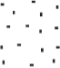
\includegraphics{area-of-coverage-2-Picture1.png}

20\% ~~~~~~~~
\includegraphics{area-of-coverage-20.png}

\hypertarget{investigation-d1-physical-weathering}{%
\section{INVESTIGATION D1: Physical
Weathering}\label{investigation-d1-physical-weathering}}

Physical weathering involves mechanical processes by which rocks exposed
to weathering break down into smaller rocks or to their constituent
minerals. Smaller rocks and particles are more susceptible to chemical
weathering. Note that some sources of physical weathering can also be
involved in chemical weathering.

\begin{itemize}
\item
  \textbf{Abrasion}: Water carrying suspended rock fragments has a
  scouring action on surfaces. Examples are the grinding action of
  glaciers, gravel, pebbles and boulders moved along and constantly
  abraded by fast-flowing streams. Particles carried by wind also have a
  ``sand-blasting'' effect.
\item
  \textbf{Wetting and drying}: Water penetrates into rocks and reacts
  with their constituent minerals resulting in recrystallization and
  increased stress. Wetting and drying is sometimes accompanied by
  shrinking and swelling, which also increasing internal stress.
\item
  \textbf{Freezing and thawing}: When water is trapped in the rock (or
  in cracks) repeated freezing and thawing results in forces of
  expansion and contraction (when water freezes, its volume increases by
  about 9 \%).
\item
  \textbf{Heating and cooling}: Each different mineral in the rock will
  expand and contract by a different amount and at a different rate with
  surface-temperature fluctuations. With time, the stresses produced are
  sufficient to weaken the bonds along grain boundaries resulting in
  flaking off of rock fragments at the rock's surface.
\item
  \textbf{Unloading/Exfoliation}: Many rocks are formed at great depth
  under intense temperatures and pressures. As these rocks make their
  way to the surface and overlying rock is removed through erosion, some
  of the pressure is released. This release of pressure causes the rock
  to fracture horizontally. Cracks of this type increase in number as
  the rock reaches the surface.
\end{itemize}

Observe the examples of physical weathering, then complete the table
below. Record ONE POTENTIAL weathering process for each example and give
a brief description of the process.

 
  \providecommand{\huxb}[2]{\arrayrulecolor[RGB]{#1}\global\arrayrulewidth=#2pt}
  \providecommand{\huxvb}[2]{\color[RGB]{#1}\vrule width #2pt}
  \providecommand{\huxtpad}[1]{\rule{0pt}{#1}}
  \providecommand{\huxbpad}[1]{\rule[-#1]{0pt}{#1}}

\begin{table}[h!]
\begin{centerbox}
\begin{threeparttable}
 
\setlength{\tabcolsep}{0pt}
\begin{tabularx}{0.9\textwidth}{p{0.45\textwidth} p{0.45\textwidth}}


\hhline{>{\huxb{0, 0, 0}{1}}->{\huxb{0, 0, 0}{1}}-}
\arrayrulecolor{black}

\multicolumn{1}{!{\huxvb{0, 0, 0}{1}}m{0.45\textwidth}!{\huxvb{0, 0, 0}{1}}}{\hspace{0pt}\parbox[c]{0.45\textwidth-0pt-4pt}{\huxtpad{0pt + 1em}\centering \textbf{Example}\huxbpad{4pt}}} &
\multicolumn{1}{m{0.45\textwidth}!{\huxvb{0, 0, 0}{1}}}{\hspace{4pt}\parbox[c]{0.45\textwidth-4pt-0pt}{\huxtpad{0pt + 1em}\centering \textbf{Physical Weathering Observations}\huxbpad{4pt}}} \tabularnewline[-0.5pt]


\hhline{>{\huxb{0, 0, 0}{1}}->{\huxb{0, 0, 0}{1}}-}
\arrayrulecolor{black}

\multicolumn{1}{!{\huxvb{0, 0, 0}{1}}m{0.45\textwidth}!{\huxvb{0, 0, 0}{1}}}{\hspace{0pt}\parbox[c]{0.45\textwidth-0pt-4pt}{\huxtpad{20pt + 1em}\centering 1\huxbpad{20pt}}} &
\multicolumn{1}{m{0.45\textwidth}!{\huxvb{0, 0, 0}{1}}}{\hspace{4pt}\parbox[c]{0.45\textwidth-4pt-0pt}{\huxtpad{20pt + 1em}\centering \huxbpad{20pt}}} \tabularnewline[-0.5pt]


\hhline{>{\huxb{0, 0, 0}{1}}->{\huxb{0, 0, 0}{1}}-}
\arrayrulecolor{black}

\multicolumn{1}{!{\huxvb{0, 0, 0}{1}}m{0.45\textwidth}!{\huxvb{0, 0, 0}{1}}}{\hspace{0pt}\parbox[c]{0.45\textwidth-0pt-4pt}{\huxtpad{20pt + 1em}\centering 2\huxbpad{20pt}}} &
\multicolumn{1}{m{0.45\textwidth}!{\huxvb{0, 0, 0}{1}}}{\hspace{4pt}\parbox[c]{0.45\textwidth-4pt-0pt}{\huxtpad{20pt + 1em}\centering \huxbpad{20pt}}} \tabularnewline[-0.5pt]


\hhline{>{\huxb{0, 0, 0}{1}}->{\huxb{0, 0, 0}{1}}-}
\arrayrulecolor{black}

\multicolumn{1}{!{\huxvb{0, 0, 0}{1}}m{0.45\textwidth}!{\huxvb{0, 0, 0}{1}}}{\hspace{0pt}\parbox[c]{0.45\textwidth-0pt-4pt}{\huxtpad{20pt + 1em}\centering 3\huxbpad{20pt}}} &
\multicolumn{1}{m{0.45\textwidth}!{\huxvb{0, 0, 0}{1}}}{\hspace{4pt}\parbox[c]{0.45\textwidth-4pt-0pt}{\huxtpad{20pt + 1em}\centering \huxbpad{20pt}}} \tabularnewline[-0.5pt]


\hhline{>{\huxb{0, 0, 0}{1}}->{\huxb{0, 0, 0}{1}}-}
\arrayrulecolor{black}

\multicolumn{1}{!{\huxvb{0, 0, 0}{1}}m{0.45\textwidth}!{\huxvb{0, 0, 0}{1}}}{\hspace{0pt}\parbox[c]{0.45\textwidth-0pt-4pt}{\huxtpad{20pt + 1em}\centering 4\huxbpad{20pt}}} &
\multicolumn{1}{m{0.45\textwidth}!{\huxvb{0, 0, 0}{1}}}{\hspace{4pt}\parbox[c]{0.45\textwidth-4pt-0pt}{\huxtpad{20pt + 1em}\centering \huxbpad{20pt}}} \tabularnewline[-0.5pt]


\hhline{>{\huxb{0, 0, 0}{1}}->{\huxb{0, 0, 0}{1}}-}
\arrayrulecolor{black}
\end{tabularx}
\end{threeparttable}\par\end{centerbox}

\end{table}
 

\hypertarget{investigation-d2-chemical-weathering}{%
\section{INVESTIGATION D2: Chemical
Weathering}\label{investigation-d2-chemical-weathering}}

Chemical weathering involves chemical processes by which rocks and
minerals exposed to the weather undergo changes in composition or
crystallinity, or are removed from the rock.

\begin{itemize}
\item
  \textbf{Hydration}: Ions have the tendency to attract water molecules
  (hydrate) and dissociate when water is present. This kind of
  weathering happens in arid environments where salts are present.
\item
  \textbf{Hydrolysis}: Water molecules at the rock's mineral surface
  dissociate into H+ and OH-- and the mobile H+ ions penetrate the
  rock's crystal lattice. This creates a charge imbalance that causes
  cations (e.g.~Ca2+, Mg2+, K+ and Na+) to diffuse out.
\item
  \textbf{Oxidation-Reduction}: Several primary minerals contain Fe2+
  and Mn2+. In an oxidizing environment, Fe2+ is oxidized to Fe3+. The
  change in oxidation state changes the size of the ion resulting in
  internal stresses and accelerated weathering. Reduced iron (Fe2+) is
  soluble and can be removed from the rock or mineral, while oxidized
  iron (Fe3+) is insoluble and remains in place.
\item
  \textbf{Dissolution}: Occurs when the component minerals of rocks are
  dissolved by water. The dissolved material is transported away leaving
  a space in the rock.
\item
  \textbf{Acidification}: Dissolving of calcium carbonate (limestone) in
  acidic groundwater. One consequence of this process is the formation
  of caves in limestone areas.
\end{itemize}

Observe the examples of chemical weathering then complete the table
below. Record ONE POTENTIAL weathering process for each example and give
a brief description of the process.

 
  \providecommand{\huxb}[2]{\arrayrulecolor[RGB]{#1}\global\arrayrulewidth=#2pt}
  \providecommand{\huxvb}[2]{\color[RGB]{#1}\vrule width #2pt}
  \providecommand{\huxtpad}[1]{\rule{0pt}{#1}}
  \providecommand{\huxbpad}[1]{\rule[-#1]{0pt}{#1}}

\begin{table}[h!]
\begin{centerbox}
\begin{threeparttable}
 
\setlength{\tabcolsep}{0pt}
\begin{tabularx}{0.9\textwidth}{p{0.45\textwidth} p{0.45\textwidth}}


\hhline{>{\huxb{0, 0, 0}{1}}->{\huxb{0, 0, 0}{1}}-}
\arrayrulecolor{black}

\multicolumn{1}{!{\huxvb{0, 0, 0}{1}}m{0.45\textwidth}!{\huxvb{0, 0, 0}{1}}}{\hspace{0pt}\parbox[c]{0.45\textwidth-0pt-4pt}{\huxtpad{0pt + 1em}\centering \textbf{Example}\huxbpad{4pt}}} &
\multicolumn{1}{m{0.45\textwidth}!{\huxvb{0, 0, 0}{1}}}{\hspace{4pt}\parbox[c]{0.45\textwidth-4pt-0pt}{\huxtpad{0pt + 1em}\centering \textbf{Chemical Weathering Observations}\huxbpad{4pt}}} \tabularnewline[-0.5pt]


\hhline{>{\huxb{0, 0, 0}{1}}->{\huxb{0, 0, 0}{1}}-}
\arrayrulecolor{black}

\multicolumn{1}{!{\huxvb{0, 0, 0}{1}}m{0.45\textwidth}!{\huxvb{0, 0, 0}{1}}}{\hspace{0pt}\parbox[c]{0.45\textwidth-0pt-4pt}{\huxtpad{20pt + 1em}\centering 1\huxbpad{20pt}}} &
\multicolumn{1}{m{0.45\textwidth}!{\huxvb{0, 0, 0}{1}}}{\hspace{4pt}\parbox[c]{0.45\textwidth-4pt-0pt}{\huxtpad{20pt + 1em}\centering \huxbpad{20pt}}} \tabularnewline[-0.5pt]


\hhline{>{\huxb{0, 0, 0}{1}}->{\huxb{0, 0, 0}{1}}-}
\arrayrulecolor{black}

\multicolumn{1}{!{\huxvb{0, 0, 0}{1}}m{0.45\textwidth}!{\huxvb{0, 0, 0}{1}}}{\hspace{0pt}\parbox[c]{0.45\textwidth-0pt-4pt}{\huxtpad{20pt + 1em}\centering 2\huxbpad{20pt}}} &
\multicolumn{1}{m{0.45\textwidth}!{\huxvb{0, 0, 0}{1}}}{\hspace{4pt}\parbox[c]{0.45\textwidth-4pt-0pt}{\huxtpad{20pt + 1em}\centering \huxbpad{20pt}}} \tabularnewline[-0.5pt]


\hhline{>{\huxb{0, 0, 0}{1}}->{\huxb{0, 0, 0}{1}}-}
\arrayrulecolor{black}

\multicolumn{1}{!{\huxvb{0, 0, 0}{1}}m{0.45\textwidth}!{\huxvb{0, 0, 0}{1}}}{\hspace{0pt}\parbox[c]{0.45\textwidth-0pt-4pt}{\huxtpad{20pt + 1em}\centering 3\huxbpad{20pt}}} &
\multicolumn{1}{m{0.45\textwidth}!{\huxvb{0, 0, 0}{1}}}{\hspace{4pt}\parbox[c]{0.45\textwidth-4pt-0pt}{\huxtpad{20pt + 1em}\centering \huxbpad{20pt}}} \tabularnewline[-0.5pt]


\hhline{>{\huxb{0, 0, 0}{1}}->{\huxb{0, 0, 0}{1}}-}
\arrayrulecolor{black}
\end{tabularx}
\end{threeparttable}\par\end{centerbox}

\end{table}
 

\hypertarget{investigation-d3-physical-weathering}{%
\section{INVESTIGATION D3: Physical
Weathering}\label{investigation-d3-physical-weathering}}

Biological weathering involves physical and chemical processes by which
organisms weather rocks.

\begin{itemize}
\item
  \textbf{Plant roots}: Woody plant rots, especially trees, can
  preferentially grow into fissures in rocks and split them apart as the
  roots grw and expand.
\item
  \textbf{Digging and crushing by animals}: Animals (including humans)
  assist in the physical breakdown of rocks by digging burrows,
  bioturbation, or even purposely crushing rock materials such as in
  many human activities.
\item
  \textbf{Lichen}: Lichen play an important part in chemical weathering
  because they producing organic acids that act as chelating (chelate =
  claw, it is a compounds that ``grabs'' elements such as Fe) agents
  that trap the insoluble elements of the decomposing rock in soluble
  organo-metallic complexes and destroy the crystal structure of the
  component minerals.
\end{itemize}

Observe the examples of biological weathering then complete the table
below. Record ONE POTENTIAL weathering process for each example and give
a brief description of the process.

 
  \providecommand{\huxb}[2]{\arrayrulecolor[RGB]{#1}\global\arrayrulewidth=#2pt}
  \providecommand{\huxvb}[2]{\color[RGB]{#1}\vrule width #2pt}
  \providecommand{\huxtpad}[1]{\rule{0pt}{#1}}
  \providecommand{\huxbpad}[1]{\rule[-#1]{0pt}{#1}}

\begin{table}[h!]
\begin{centerbox}
\begin{threeparttable}
 
\setlength{\tabcolsep}{0pt}
\begin{tabularx}{0.9\textwidth}{p{0.45\textwidth} p{0.45\textwidth}}


\hhline{>{\huxb{0, 0, 0}{1}}->{\huxb{0, 0, 0}{1}}-}
\arrayrulecolor{black}

\multicolumn{1}{!{\huxvb{0, 0, 0}{1}}m{0.45\textwidth}!{\huxvb{0, 0, 0}{1}}}{\hspace{0pt}\parbox[c]{0.45\textwidth-0pt-4pt}{\huxtpad{0pt + 1em}\centering \textbf{Example}\huxbpad{4pt}}} &
\multicolumn{1}{m{0.45\textwidth}!{\huxvb{0, 0, 0}{1}}}{\hspace{4pt}\parbox[c]{0.45\textwidth-4pt-0pt}{\huxtpad{0pt + 1em}\centering \textbf{Biological Weathering Observations}\huxbpad{4pt}}} \tabularnewline[-0.5pt]


\hhline{>{\huxb{0, 0, 0}{1}}->{\huxb{0, 0, 0}{1}}-}
\arrayrulecolor{black}

\multicolumn{1}{!{\huxvb{0, 0, 0}{1}}m{0.45\textwidth}!{\huxvb{0, 0, 0}{1}}}{\hspace{0pt}\parbox[c]{0.45\textwidth-0pt-4pt}{\huxtpad{20pt + 1em}\centering 1\huxbpad{20pt}}} &
\multicolumn{1}{m{0.45\textwidth}!{\huxvb{0, 0, 0}{1}}}{\hspace{4pt}\parbox[c]{0.45\textwidth-4pt-0pt}{\huxtpad{20pt + 1em}\centering \huxbpad{20pt}}} \tabularnewline[-0.5pt]


\hhline{>{\huxb{0, 0, 0}{1}}->{\huxb{0, 0, 0}{1}}-}
\arrayrulecolor{black}

\multicolumn{1}{!{\huxvb{0, 0, 0}{1}}m{0.45\textwidth}!{\huxvb{0, 0, 0}{1}}}{\hspace{0pt}\parbox[c]{0.45\textwidth-0pt-4pt}{\huxtpad{20pt + 1em}\centering 2\huxbpad{20pt}}} &
\multicolumn{1}{m{0.45\textwidth}!{\huxvb{0, 0, 0}{1}}}{\hspace{4pt}\parbox[c]{0.45\textwidth-4pt-0pt}{\huxtpad{20pt + 1em}\centering \huxbpad{20pt}}} \tabularnewline[-0.5pt]


\hhline{>{\huxb{0, 0, 0}{1}}->{\huxb{0, 0, 0}{1}}-}
\arrayrulecolor{black}
\end{tabularx}
\end{threeparttable}\par\end{centerbox}

\end{table}
 

\hypertarget{investigation-e-weathering-examples}{%
\section{INVESTIGATION E: Weathering
Examples}\label{investigation-e-weathering-examples}}

\begin{enumerate}
\def\labelenumi{\arabic{enumi}.}
\tightlist
\item
  Using an eye dropper, apply a drop of 10\% hydrochloric acid to the
  limestone rock located in the test plates.
\end{enumerate}

\begin{enumerate}
\def\labelenumi{\alph{enumi}.}
\tightlist
\item
  Describe what you see when the acid makes contact with the limestone
  rock.
\end{enumerate}

~ ~ ~

\begin{enumerate}
\def\labelenumi{\alph{enumi}.}
\setcounter{enumi}{1}
\tightlist
\item
  Describe what happens to the rock.
\end{enumerate}

~ ~ ~

\begin{enumerate}
\def\labelenumi{\alph{enumi}.}
\setcounter{enumi}{2}
\tightlist
\item
  What type of weathering does this represent?
\end{enumerate}

~ ~ ~

\begin{enumerate}
\def\labelenumi{\arabic{enumi}.}
\setcounter{enumi}{1}
\tightlist
\item
  These two salt samples (NaCl crystals; common table salt) were equal
  in size at the beginning of this experiment. Using the squirt bottle,
  apply a stream of water to an edge or corner of the salt block on the
  left.
\end{enumerate}

\begin{enumerate}
\def\labelenumi{\alph{enumi}.}
\tightlist
\item
  Describe what you see when the water makes contact with the salt.
\end{enumerate}

~ ~ ~

\begin{enumerate}
\def\labelenumi{\alph{enumi}.}
\setcounter{enumi}{1}
\tightlist
\item
  Describe what happens to the salt block.
\end{enumerate}

~ ~ ~

\begin{enumerate}
\def\labelenumi{\alph{enumi}.}
\setcounter{enumi}{2}
\tightlist
\item
  What type of weathering does this represent?
\end{enumerate}

~ ~ ~

\begin{enumerate}
\def\labelenumi{\arabic{enumi}.}
\setcounter{enumi}{2}
\tightlist
\item
  How might physical weathering help promote chemical weathering?
\end{enumerate}

~ ~ ~

\hypertarget{investigation-f-naming-master-horizons---review}{%
\section{INVESTIGATION F: Naming Master Horizons -
Review}\label{investigation-f-naming-master-horizons---review}}

Observe the six mini-monoliths on the table. The monoliths are scaled so
that one inch on a monolith equals four inches on a soil profile. Label
the master horizons and the mark depths of these horizons for monoliths
2 through 3. Monolith 1 is done for you. Note that horizon depth is
always measured from the soil surface. All profiles are 48'' deep. NOTE:
There are no ``O'' (organic) horizons in this investigation.

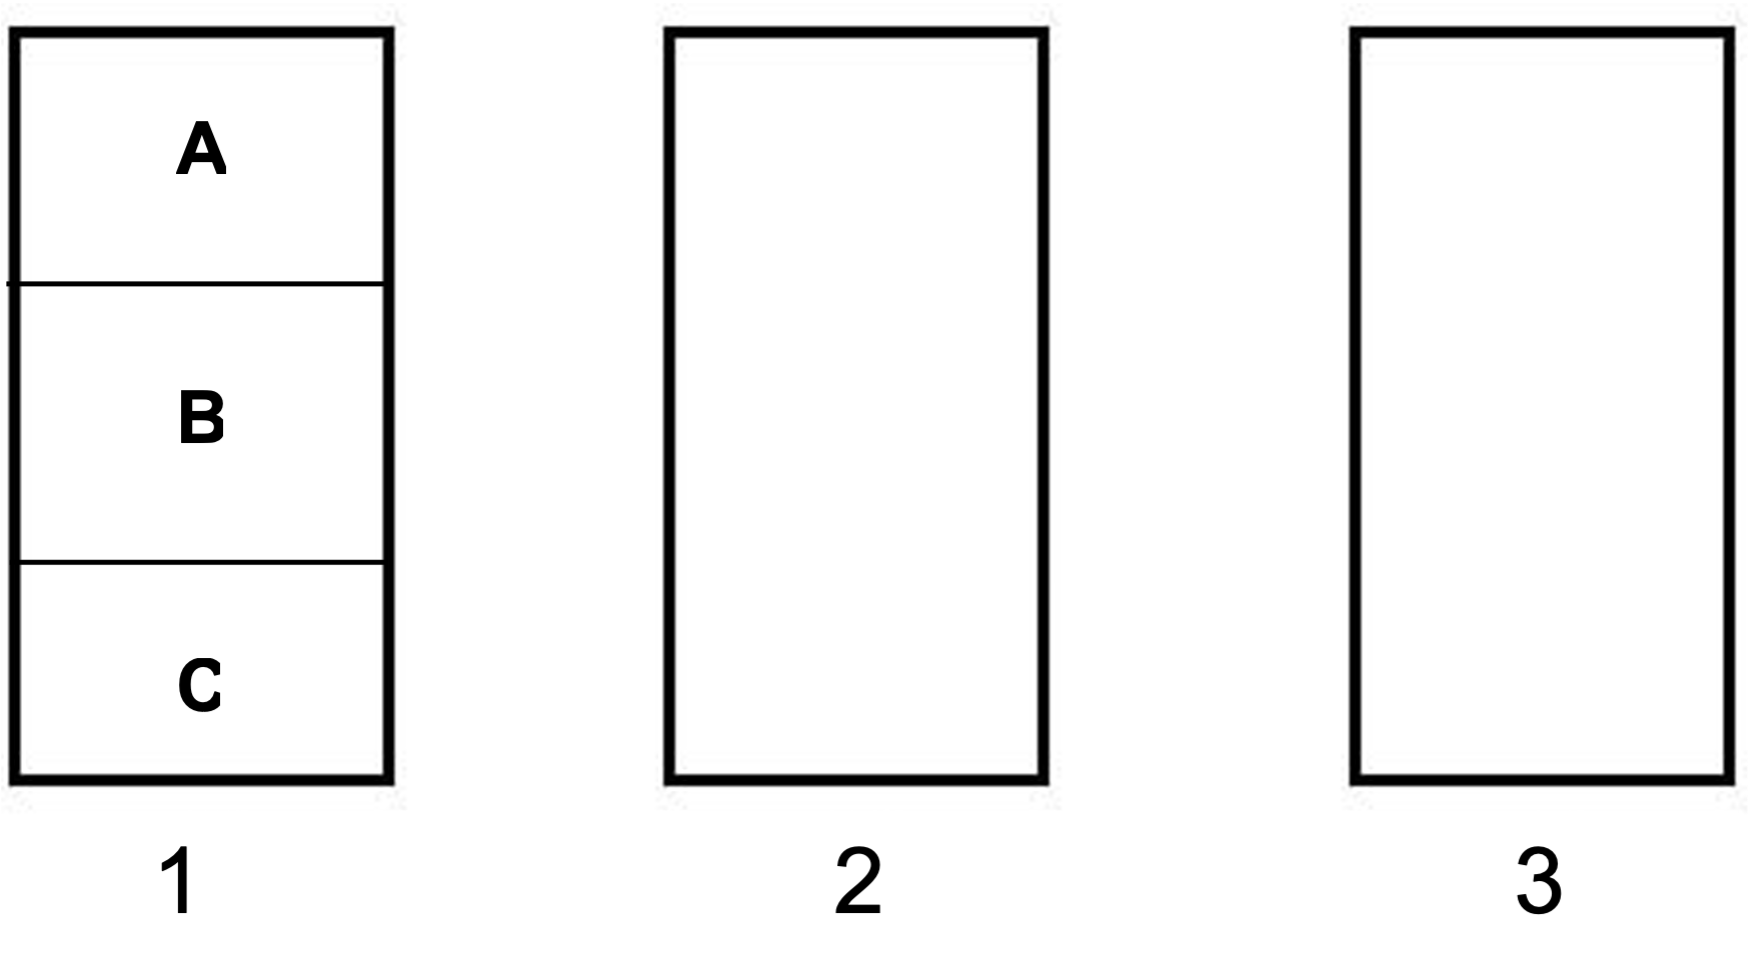
\includegraphics{naming-master-horizons-Picture1.png} \textbf{Remember:
1 monolith inch = 4 soil profile inches}

\bookmarksetup{startatroot}

\hypertarget{five-soil-forming-factors}{%
\chapter{\texorpdfstring{\textbf{Five Soil Forming
Factors}}{Five Soil Forming Factors}}\label{five-soil-forming-factors}}

\begin{tcolorbox}[enhanced jigsaw, colframe=quarto-callout-note-color-frame, coltitle=black, arc=.35mm, breakable, bottomrule=.15mm, colback=white, rightrule=.15mm, toprule=.15mm, opacityback=0, bottomtitle=1mm, left=2mm, titlerule=0mm, leftrule=.75mm, opacitybacktitle=0.6, toptitle=1mm, title=\textcolor{quarto-callout-note-color}{\faInfo}\hspace{0.5em}{Objectives}, colbacktitle=quarto-callout-note-color!10!white]

\begin{itemize}
\tightlist
\item
  To understand the interaction of soil forming factors and the soil
  forming processes in the formation and evolution of soils. Soils will
  develop different characteristics due to the action of climate and
  biotic factors acting on a parent material on a particular landscape
  position over time. The additions, losses, translocations, and
  transformations to the soil profile develop soil horizons.
\end{itemize}

\end{tcolorbox}

\begin{tcolorbox}[enhanced jigsaw, colframe=quarto-callout-tip-color-frame, coltitle=black, arc=.35mm, breakable, bottomrule=.15mm, colback=white, rightrule=.15mm, toprule=.15mm, opacityback=0, bottomtitle=1mm, left=2mm, titlerule=0mm, leftrule=.75mm, opacitybacktitle=0.6, toptitle=1mm, title=\textcolor{quarto-callout-tip-color}{\faLightbulb}\hspace{0.5em}{Key Words \& Concepts}, colbacktitle=quarto-callout-tip-color!10!white]

\begin{itemize}
\tightlist
\item
  Residuum
\item
  Catena
\item
  Soil ``age''
\item
  Lacustrine
\item
  Alluvial
\item
  Till
\item
  Eolian
\item
  Loess
\item
  Calcareous
\item
  Colluvial
\item
  Esker
\item
  Moraine
\item
  Leaching
\item
  Evapotranspiration
\item
  Native vegetation
\item
  Erosion
\item
  Deposition
\item
  Aspect
\item
  Horizonation
\item
  Backslope
\item
  Summit
\item
  Shoulder
\item
  Footslope
\item
  Infiltration
\item
  Drainage classes
\item
  Mottles
\item
  Sesquioxides
\end{itemize}

\end{tcolorbox}

\hypertarget{investigation-a-residual-parent-materials}{%
\section{INVESTIGATION A: Residual Parent
Materials}\label{investigation-a-residual-parent-materials}}

Soils develop in many different kinds of parent materials. Parent
material, in some cases, can be the bedrock under the soil and this
non-transported parent material is called residuum. The soils that
develop in residuum can be shallow if the rock is hard and difficult to
weather, or deep if the rock is soft or has weathered for a long time.
In Minnesota, four types of bedrock can be located that are only thinly
or not covered by glacial drift and thus can become residual parent
material--- limestone, sandstone, basalt, and granite. Use the depth to
bedrock map and simplified geological map to describe the most likely
rock type for residual soils at points A, B and C.

\begin{figure}

{\centering 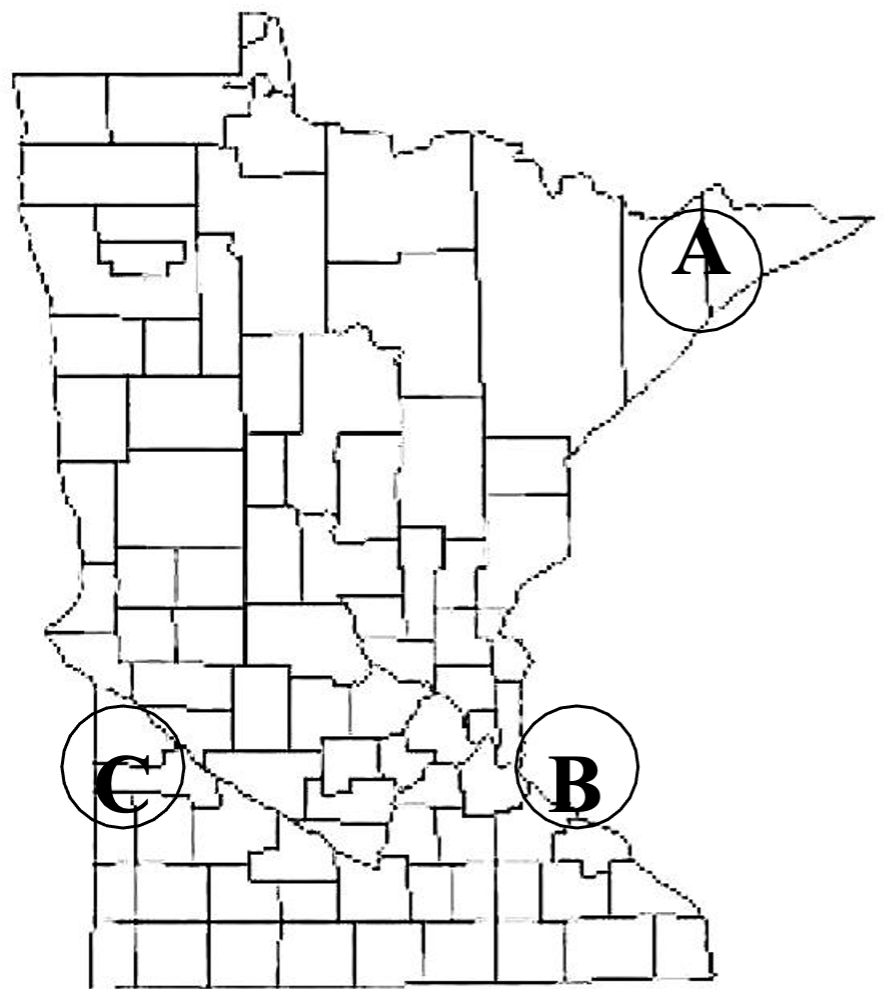
\includegraphics{residual-parent-materials-Picture1.png}

}

\caption{\label{fig-residual}Minnesota}

\end{figure}

A: ~~~~~~~~~~~~~~~~~~~~~~~~~~~~~~~~~~~~~~~ ~~~~~~~~~~~~~~~~B:
~~~~~~~~~~~~~~~~~~~~~~~~~~~~~~~~~~~~~~~~~~~~~~~~~~~~~~~C:

\hypertarget{investigation-b-clay-mineral-block-structures-1}{%
\section{INVESTIGATION B: Clay Mineral Block
Structures}\label{investigation-b-clay-mineral-block-structures-1}}

In Minnesota, most soils are formed in a parent material that was
transported by ice, wind or water. Ice deposited glacial till, water
deposited glacial outwash, glacial lacustrine and alluvium, and wind
deposited eolian sand and loess. Observe the samples of transported
parent materials and note characteristics for each sample. These
characteristics (particularly color and texture) are very useful for
identifying the parent material of many Minnesota soils.

 
  \providecommand{\huxb}[2]{\arrayrulecolor[RGB]{#1}\global\arrayrulewidth=#2pt}
  \providecommand{\huxvb}[2]{\color[RGB]{#1}\vrule width #2pt}
  \providecommand{\huxtpad}[1]{\rule{0pt}{#1}}
  \providecommand{\huxbpad}[1]{\rule[-#1]{0pt}{#1}}

\begin{table}[h!]
\begin{centerbox}
\begin{threeparttable}
 
\setlength{\tabcolsep}{0pt}
\begin{tabularx}{0.9\textwidth}{p{0.45\textwidth} p{0.45\textwidth}}


\hhline{>{\huxb{0, 0, 0}{1}}->{\huxb{0, 0, 0}{1}}-}
\arrayrulecolor{black}

\multicolumn{1}{!{\huxvb{0, 0, 0}{1}}m{0.45\textwidth}!{\huxvb{0, 0, 0}{1}}}{\hspace{0pt}\parbox[c]{0.45\textwidth-0pt-4pt}{\huxtpad{0pt + 1em}\centering \textbf{GLACIAL TILL}\huxbpad{4pt}}} &
\multicolumn{1}{m{0.45\textwidth}!{\huxvb{0, 0, 0}{1}}}{\hspace{4pt}\parbox[c]{0.45\textwidth-4pt-0pt}{\huxtpad{0pt + 1em}\centering \textbf{Observed Characteristics (Color, texture, coarse fragments)}\huxbpad{4pt}}} \tabularnewline[-0.5pt]


\hhline{>{\huxb{0, 0, 0}{1}}->{\huxb{0, 0, 0}{1}}-}
\arrayrulecolor{black}

\multicolumn{1}{!{\huxvb{0, 0, 0}{1}}m{0.45\textwidth}!{\huxvb{0, 0, 0}{1}}}{\hspace{0pt}\parbox[c]{0.45\textwidth-0pt-4pt}{\huxtpad{40pt + 1em}\centering Superior Lobe Till\huxbpad{40pt}}} &
\multicolumn{1}{m{0.45\textwidth}!{\huxvb{0, 0, 0}{1}}}{\hspace{4pt}\parbox[c]{0.45\textwidth-4pt-0pt}{\huxtpad{40pt + 1em}\centering \huxbpad{40pt}}} \tabularnewline[-0.5pt]


\hhline{>{\huxb{0, 0, 0}{1}}->{\huxb{0, 0, 0}{1}}-}
\arrayrulecolor{black}

\multicolumn{1}{!{\huxvb{0, 0, 0}{1}}m{0.45\textwidth}!{\huxvb{0, 0, 0}{1}}}{\hspace{0pt}\parbox[c]{0.45\textwidth-0pt-4pt}{\huxtpad{40pt + 1em}\centering Des Moines Lobe Till\huxbpad{40pt}}} &
\multicolumn{1}{m{0.45\textwidth}!{\huxvb{0, 0, 0}{1}}}{\hspace{4pt}\parbox[c]{0.45\textwidth-4pt-0pt}{\huxtpad{40pt + 1em}\centering \huxbpad{40pt}}} \tabularnewline[-0.5pt]


\hhline{>{\huxb{0, 0, 0}{1}}->{\huxb{0, 0, 0}{1}}-}
\arrayrulecolor{black}
\end{tabularx}
\end{threeparttable}\par\end{centerbox}

\end{table}
 

 
  \providecommand{\huxb}[2]{\arrayrulecolor[RGB]{#1}\global\arrayrulewidth=#2pt}
  \providecommand{\huxvb}[2]{\color[RGB]{#1}\vrule width #2pt}
  \providecommand{\huxtpad}[1]{\rule{0pt}{#1}}
  \providecommand{\huxbpad}[1]{\rule[-#1]{0pt}{#1}}

\begin{table}[h!]
\begin{centerbox}
\begin{threeparttable}
 
\setlength{\tabcolsep}{0pt}
\begin{tabularx}{0.9\textwidth}{p{0.45\textwidth} p{0.45\textwidth}}


\hhline{>{\huxb{0, 0, 0}{1}}->{\huxb{0, 0, 0}{1}}-}
\arrayrulecolor{black}

\multicolumn{1}{!{\huxvb{0, 0, 0}{1}}m{0.45\textwidth}!{\huxvb{0, 0, 0}{1}}}{\hspace{0pt}\parbox[c]{0.45\textwidth-0pt-4pt}{\huxtpad{0pt + 1em}\centering \textbf{WATER SORTED}\huxbpad{4pt}}} &
\multicolumn{1}{m{0.45\textwidth}!{\huxvb{0, 0, 0}{1}}}{\hspace{4pt}\parbox[c]{0.45\textwidth-4pt-0pt}{\huxtpad{0pt + 1em}\centering \textbf{Observed Characteristics (Color, texture, coarse fragments)}\huxbpad{4pt}}} \tabularnewline[-0.5pt]


\hhline{>{\huxb{0, 0, 0}{1}}->{\huxb{0, 0, 0}{1}}-}
\arrayrulecolor{black}

\multicolumn{1}{!{\huxvb{0, 0, 0}{1}}m{0.45\textwidth}!{\huxvb{0, 0, 0}{1}}}{\hspace{0pt}\parbox[c]{0.45\textwidth-0pt-4pt}{\huxtpad{40pt + 1em}\centering Lacustrine\huxbpad{40pt}}} &
\multicolumn{1}{m{0.45\textwidth}!{\huxvb{0, 0, 0}{1}}}{\hspace{4pt}\parbox[c]{0.45\textwidth-4pt-0pt}{\huxtpad{40pt + 1em}\centering \huxbpad{40pt}}} \tabularnewline[-0.5pt]


\hhline{>{\huxb{0, 0, 0}{1}}->{\huxb{0, 0, 0}{1}}-}
\arrayrulecolor{black}

\multicolumn{1}{!{\huxvb{0, 0, 0}{1}}m{0.45\textwidth}!{\huxvb{0, 0, 0}{1}}}{\hspace{0pt}\parbox[c]{0.45\textwidth-0pt-4pt}{\huxtpad{40pt + 1em}\centering Outwash\huxbpad{40pt}}} &
\multicolumn{1}{m{0.45\textwidth}!{\huxvb{0, 0, 0}{1}}}{\hspace{4pt}\parbox[c]{0.45\textwidth-4pt-0pt}{\huxtpad{40pt + 1em}\centering \huxbpad{40pt}}} \tabularnewline[-0.5pt]


\hhline{>{\huxb{0, 0, 0}{1}}->{\huxb{0, 0, 0}{1}}-}
\arrayrulecolor{black}

\multicolumn{1}{!{\huxvb{0, 0, 0}{1}}m{0.45\textwidth}!{\huxvb{0, 0, 0}{1}}}{\hspace{0pt}\parbox[c]{0.45\textwidth-0pt-4pt}{\huxtpad{40pt + 1em}\centering Alluvium\huxbpad{40pt}}} &
\multicolumn{1}{m{0.45\textwidth}!{\huxvb{0, 0, 0}{1}}}{\hspace{4pt}\parbox[c]{0.45\textwidth-4pt-0pt}{\huxtpad{40pt + 1em}\centering \huxbpad{40pt}}} \tabularnewline[-0.5pt]


\hhline{>{\huxb{0, 0, 0}{1}}->{\huxb{0, 0, 0}{1}}-}
\arrayrulecolor{black}
\end{tabularx}
\end{threeparttable}\par\end{centerbox}

\end{table}
 

 
  \providecommand{\huxb}[2]{\arrayrulecolor[RGB]{#1}\global\arrayrulewidth=#2pt}
  \providecommand{\huxvb}[2]{\color[RGB]{#1}\vrule width #2pt}
  \providecommand{\huxtpad}[1]{\rule{0pt}{#1}}
  \providecommand{\huxbpad}[1]{\rule[-#1]{0pt}{#1}}

\begin{table}[h!]
\begin{centerbox}
\begin{threeparttable}
 
\setlength{\tabcolsep}{0pt}
\begin{tabularx}{0.9\textwidth}{p{0.45\textwidth} p{0.45\textwidth}}


\hhline{>{\huxb{0, 0, 0}{1}}->{\huxb{0, 0, 0}{1}}-}
\arrayrulecolor{black}

\multicolumn{1}{!{\huxvb{0, 0, 0}{1}}m{0.45\textwidth}!{\huxvb{0, 0, 0}{1}}}{\hspace{0pt}\parbox[c]{0.45\textwidth-0pt-4pt}{\huxtpad{0pt + 1em}\centering \textbf{WIND SORTED}\huxbpad{4pt}}} &
\multicolumn{1}{m{0.45\textwidth}!{\huxvb{0, 0, 0}{1}}}{\hspace{4pt}\parbox[c]{0.45\textwidth-4pt-0pt}{\huxtpad{0pt + 1em}\centering \textbf{Observed Characteristics (Color, texture, coarse fragments)}\huxbpad{4pt}}} \tabularnewline[-0.5pt]


\hhline{>{\huxb{0, 0, 0}{1}}->{\huxb{0, 0, 0}{1}}-}
\arrayrulecolor{black}

\multicolumn{1}{!{\huxvb{0, 0, 0}{1}}m{0.45\textwidth}!{\huxvb{0, 0, 0}{1}}}{\hspace{0pt}\parbox[c]{0.45\textwidth-0pt-4pt}{\huxtpad{40pt + 1em}\centering Dune sand (eolian; transported very locally by wind)\huxbpad{40pt}}} &
\multicolumn{1}{m{0.45\textwidth}!{\huxvb{0, 0, 0}{1}}}{\hspace{4pt}\parbox[c]{0.45\textwidth-4pt-0pt}{\huxtpad{40pt + 1em}\centering \huxbpad{40pt}}} \tabularnewline[-0.5pt]


\hhline{>{\huxb{0, 0, 0}{1}}->{\huxb{0, 0, 0}{1}}-}
\arrayrulecolor{black}

\multicolumn{1}{!{\huxvb{0, 0, 0}{1}}m{0.45\textwidth}!{\huxvb{0, 0, 0}{1}}}{\hspace{0pt}\parbox[c]{0.45\textwidth-0pt-4pt}{\huxtpad{40pt + 1em}\centering Loess\huxbpad{40pt}}} &
\multicolumn{1}{m{0.45\textwidth}!{\huxvb{0, 0, 0}{1}}}{\hspace{4pt}\parbox[c]{0.45\textwidth-4pt-0pt}{\huxtpad{40pt + 1em}\centering \huxbpad{40pt}}} \tabularnewline[-0.5pt]


\hhline{>{\huxb{0, 0, 0}{1}}->{\huxb{0, 0, 0}{1}}-}
\arrayrulecolor{black}
\end{tabularx}
\end{threeparttable}\par\end{centerbox}

\end{table}
 

\hypertarget{investigation-c-climatic-factors}{%
\section{INVESTIGATION C: Climatic
Factors}\label{investigation-c-climatic-factors}}

Climate refers to the amount of precipitation (rain, snow, humidity) and
the temperature in a given locale. The hotter and more humid a climate,
the faster and more completely it is going to weather into soil. If a
climate is cool and or dry, the weathering process proceeds more slowly.
Below are temperature and precipitation maps for Minnesota. The
difference in temperature will not change the weathering of rocks in
Minnesota. However, the precipitation and temperature together will
influence the leaching and horizon formation. Calcium carbonate will
occur closer to the surface in soils with less leaching as in western
Minnesota. NOTE: The diagram below shows the general pattern but DOES
NOT correspond to the exact depth of leaching for any one particular
profile.

\begin{enumerate}
\def\labelenumi{\arabic{enumi}.}
\tightlist
\item
  Match each soil profile with its location in Minnesota by the depth to
  CaCO3 (Bk or Ck). Use HCl to determine depths to carbonates.
\end{enumerate}

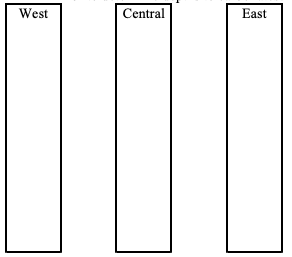
\includegraphics{depth-to-carbonates.png}
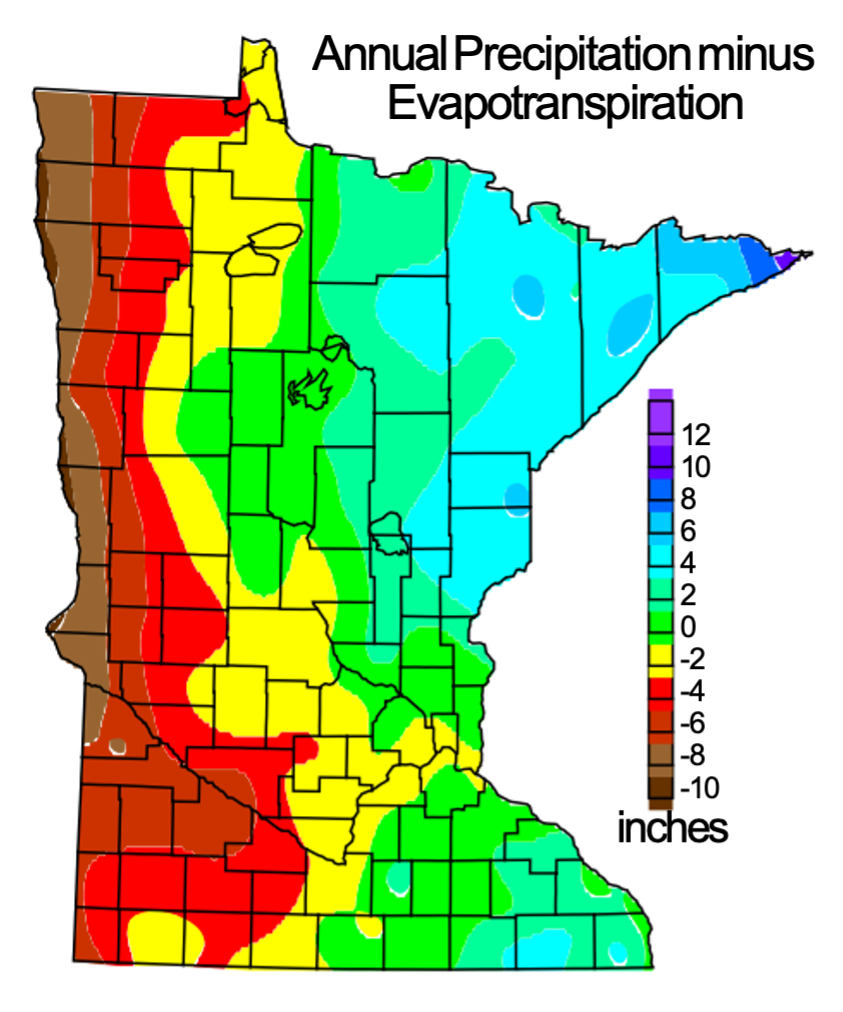
\includegraphics{mn-precip-evap.png}

\begin{enumerate}
\def\labelenumi{\arabic{enumi}.}
\setcounter{enumi}{1}
\tightlist
\item
  For a more detailed and complex representation of the depth to
  carbonates in soils across Minnesota, see the depth to carbonates map
  in Soil Explorer on the iPads. In addition to climate, which two of
  the other four soil forming factors contribute the most to these
  patterns, and why?
\end{enumerate}

~ ~ ~ ~ ~

\hypertarget{investigation-d-biotic-factors-vegetation}{%
\section{INVESTIGATION D: Biotic Factors
(Vegetation)}\label{investigation-d-biotic-factors-vegetation}}

One of the most obvious biotic factors is the effect that vegetation has
on soil formation. The most common pre-European settlement vegetative
types (this is the vegetation the soil formed under for
\textasciitilde{} 10,000 -- 13,000 years after glaciation -- the native
vegetation in many areas has been replaced by agriculture or other land
uses, but only very recently) in Minnesota are forest, grassland
(prairie), and a transitional zone between forest and grassland prairie
(called savannah). Using the six micro-monoliths(1/4 scale), determine
the vegetation that the following soils were formed under, and briefly
explain your answer.

 
  \providecommand{\huxb}[2]{\arrayrulecolor[RGB]{#1}\global\arrayrulewidth=#2pt}
  \providecommand{\huxvb}[2]{\color[RGB]{#1}\vrule width #2pt}
  \providecommand{\huxtpad}[1]{\rule{0pt}{#1}}
  \providecommand{\huxbpad}[1]{\rule[-#1]{0pt}{#1}}

\begin{table}[h!]
\begin{centerbox}
\begin{threeparttable}
 
\setlength{\tabcolsep}{0pt}
\begin{tabularx}{0.9\textwidth}{p{0.3\textwidth} p{0.3\textwidth} p{0.3\textwidth}}


\hhline{>{\huxb{0, 0, 0}{1}}->{\huxb{0, 0, 0}{1}}->{\huxb{0, 0, 0}{1}}-}
\arrayrulecolor{black}

\multicolumn{1}{!{\huxvb{0, 0, 0}{1}}m{0.3\textwidth}!{\huxvb{0, 0, 0}{1}}}{\hspace{0pt}\parbox[c]{0.3\textwidth-0pt-4pt}{\huxtpad{0pt + 1em}\centering \textbf{Soil}\huxbpad{4pt}}} &
\multicolumn{1}{m{0.3\textwidth}!{\huxvb{0, 0, 0}{1}}}{\hspace{4pt}\parbox[c]{0.3\textwidth-4pt-4pt}{\huxtpad{0pt + 1em}\centering \textbf{Most Likely Historic Vegetation (Forest, Prairie, or Savannah (Transition))}\huxbpad{4pt}}} &
\multicolumn{1}{m{0.3\textwidth}!{\huxvb{0, 0, 0}{1}}}{\hspace{4pt}\parbox[c]{0.3\textwidth-4pt-0pt}{\huxtpad{0pt + 1em}\centering \textbf{Explanation (1 in on monolith = 4 in actual)}\huxbpad{4pt}}} \tabularnewline[-0.5pt]


\hhline{>{\huxb{0, 0, 0}{1}}->{\huxb{0, 0, 0}{1}}->{\huxb{0, 0, 0}{1}}-}
\arrayrulecolor{black}

\multicolumn{1}{!{\huxvb{0, 0, 0}{1}}m{0.3\textwidth}!{\huxvb{0, 0, 0}{1}}}{\hspace{0pt}\parbox[c]{0.3\textwidth-0pt-4pt}{\huxtpad{40pt + 1em}\centering 1\huxbpad{40pt}}} &
\multicolumn{1}{m{0.3\textwidth}!{\huxvb{0, 0, 0}{1}}}{\hspace{4pt}\parbox[c]{0.3\textwidth-4pt-4pt}{\huxtpad{40pt + 1em}\centering \huxbpad{40pt}}} &
\multicolumn{1}{m{0.3\textwidth}!{\huxvb{0, 0, 0}{1}}}{\hspace{4pt}\parbox[c]{0.3\textwidth-4pt-0pt}{\huxtpad{4pt + 1em}\centering \huxbpad{4pt}}} \tabularnewline[-0.5pt]


\hhline{>{\huxb{0, 0, 0}{1}}->{\huxb{0, 0, 0}{1}}->{\huxb{0, 0, 0}{1}}-}
\arrayrulecolor{black}

\multicolumn{1}{!{\huxvb{0, 0, 0}{1}}m{0.3\textwidth}!{\huxvb{0, 0, 0}{1}}}{\hspace{0pt}\parbox[c]{0.3\textwidth-0pt-4pt}{\huxtpad{40pt + 1em}\centering 2\huxbpad{40pt}}} &
\multicolumn{1}{m{0.3\textwidth}!{\huxvb{0, 0, 0}{1}}}{\hspace{4pt}\parbox[c]{0.3\textwidth-4pt-4pt}{\huxtpad{40pt + 1em}\centering \huxbpad{40pt}}} &
\multicolumn{1}{m{0.3\textwidth}!{\huxvb{0, 0, 0}{1}}}{\hspace{4pt}\parbox[c]{0.3\textwidth-4pt-0pt}{\huxtpad{4pt + 1em}\centering \huxbpad{4pt}}} \tabularnewline[-0.5pt]


\hhline{>{\huxb{0, 0, 0}{1}}->{\huxb{0, 0, 0}{1}}->{\huxb{0, 0, 0}{1}}-}
\arrayrulecolor{black}

\multicolumn{1}{!{\huxvb{0, 0, 0}{1}}m{0.3\textwidth}!{\huxvb{0, 0, 0}{1}}}{\hspace{0pt}\parbox[c]{0.3\textwidth-0pt-4pt}{\huxtpad{40pt + 1em}\centering 3\huxbpad{40pt}}} &
\multicolumn{1}{m{0.3\textwidth}!{\huxvb{0, 0, 0}{1}}}{\hspace{4pt}\parbox[c]{0.3\textwidth-4pt-4pt}{\huxtpad{40pt + 1em}\centering \huxbpad{40pt}}} &
\multicolumn{1}{m{0.3\textwidth}!{\huxvb{0, 0, 0}{1}}}{\hspace{4pt}\parbox[c]{0.3\textwidth-4pt-0pt}{\huxtpad{4pt + 1em}\centering \huxbpad{4pt}}} \tabularnewline[-0.5pt]


\hhline{>{\huxb{0, 0, 0}{1}}->{\huxb{0, 0, 0}{1}}->{\huxb{0, 0, 0}{1}}-}
\arrayrulecolor{black}

\multicolumn{1}{!{\huxvb{0, 0, 0}{1}}m{0.3\textwidth}!{\huxvb{0, 0, 0}{1}}}{\hspace{0pt}\parbox[c]{0.3\textwidth-0pt-4pt}{\huxtpad{40pt + 1em}\centering 4\huxbpad{40pt}}} &
\multicolumn{1}{m{0.3\textwidth}!{\huxvb{0, 0, 0}{1}}}{\hspace{4pt}\parbox[c]{0.3\textwidth-4pt-4pt}{\huxtpad{40pt + 1em}\centering \huxbpad{40pt}}} &
\multicolumn{1}{m{0.3\textwidth}!{\huxvb{0, 0, 0}{1}}}{\hspace{4pt}\parbox[c]{0.3\textwidth-4pt-0pt}{\huxtpad{4pt + 1em}\centering \huxbpad{4pt}}} \tabularnewline[-0.5pt]


\hhline{>{\huxb{0, 0, 0}{1}}->{\huxb{0, 0, 0}{1}}->{\huxb{0, 0, 0}{1}}-}
\arrayrulecolor{black}

\multicolumn{1}{!{\huxvb{0, 0, 0}{1}}m{0.3\textwidth}!{\huxvb{0, 0, 0}{1}}}{\hspace{0pt}\parbox[c]{0.3\textwidth-0pt-4pt}{\huxtpad{40pt + 1em}\centering 5\huxbpad{40pt}}} &
\multicolumn{1}{m{0.3\textwidth}!{\huxvb{0, 0, 0}{1}}}{\hspace{4pt}\parbox[c]{0.3\textwidth-4pt-4pt}{\huxtpad{40pt + 1em}\centering \huxbpad{40pt}}} &
\multicolumn{1}{m{0.3\textwidth}!{\huxvb{0, 0, 0}{1}}}{\hspace{4pt}\parbox[c]{0.3\textwidth-4pt-0pt}{\huxtpad{4pt + 1em}\centering \huxbpad{4pt}}} \tabularnewline[-0.5pt]


\hhline{>{\huxb{0, 0, 0}{1}}->{\huxb{0, 0, 0}{1}}->{\huxb{0, 0, 0}{1}}-}
\arrayrulecolor{black}

\multicolumn{1}{!{\huxvb{0, 0, 0}{1}}m{0.3\textwidth}!{\huxvb{0, 0, 0}{1}}}{\hspace{0pt}\parbox[c]{0.3\textwidth-0pt-4pt}{\huxtpad{40pt + 1em}\centering 6\huxbpad{40pt}}} &
\multicolumn{1}{m{0.3\textwidth}!{\huxvb{0, 0, 0}{1}}}{\hspace{4pt}\parbox[c]{0.3\textwidth-4pt-4pt}{\huxtpad{40pt + 1em}\centering \huxbpad{40pt}}} &
\multicolumn{1}{m{0.3\textwidth}!{\huxvb{0, 0, 0}{1}}}{\hspace{4pt}\parbox[c]{0.3\textwidth-4pt-0pt}{\huxtpad{4pt + 1em}\centering \huxbpad{0pt}}} \tabularnewline[-0.5pt]


\hhline{>{\huxb{0, 0, 0}{1}}->{\huxb{0, 0, 0}{1}}->{\huxb{0, 0, 0}{1}}-}
\arrayrulecolor{black}
\end{tabularx}
\end{threeparttable}\par\end{centerbox}

\end{table}
 

\hypertarget{investigation-e-topographic-factors}{%
\section{INVESTIGATION E: Topographic
Factors}\label{investigation-e-topographic-factors}}

When forming within a landscape, soils with the same parent material,
vegetation, and climate often have different depths to the water table
(e.g.~are different due to topography only). This grouping of soils is
called a catena. Find and examine the Clarion, Nicollet, Webster, and
Glencoe monoliths against the elevator shaft in the display area and
determine the location of each soil on the following catena block
diagram and explain your answers.

 
  \providecommand{\huxb}[2]{\arrayrulecolor[RGB]{#1}\global\arrayrulewidth=#2pt}
  \providecommand{\huxvb}[2]{\color[RGB]{#1}\vrule width #2pt}
  \providecommand{\huxtpad}[1]{\rule{0pt}{#1}}
  \providecommand{\huxbpad}[1]{\rule[-#1]{0pt}{#1}}

\begin{table}[h!]
\begin{centerbox}
\begin{threeparttable}
 
\setlength{\tabcolsep}{0pt}
\begin{tabularx}{0.9\textwidth}{p{0.3\textwidth} p{0.3\textwidth} p{0.3\textwidth}}


\hhline{>{\huxb{0, 0, 0}{1}}->{\huxb{0, 0, 0}{1}}->{\huxb{0, 0, 0}{1}}-}
\arrayrulecolor{black}

\multicolumn{1}{!{\huxvb{0, 0, 0}{1}}m{0.3\textwidth}!{\huxvb{0, 0, 0}{1}}}{\hspace{0pt}\parbox[c]{0.3\textwidth-0pt-4pt}{\huxtpad{0pt + 1em}\centering \textbf{Topography}\huxbpad{4pt}}} &
\multicolumn{1}{m{0.3\textwidth}!{\huxvb{0, 0, 0}{1}}}{\hspace{4pt}\parbox[c]{0.3\textwidth-4pt-4pt}{\huxtpad{0pt + 1em}\centering \textbf{Soil Name}\huxbpad{4pt}}} &
\multicolumn{1}{m{0.3\textwidth}!{\huxvb{0, 0, 0}{1}}}{\hspace{4pt}\parbox[c]{0.3\textwidth-4pt-0pt}{\huxtpad{0pt + 1em}\centering \textbf{Explanation}\huxbpad{4pt}}} \tabularnewline[-0.5pt]


\hhline{>{\huxb{0, 0, 0}{1}}->{\huxb{0, 0, 0}{1}}->{\huxb{0, 0, 0}{1}}-}
\arrayrulecolor{black}

\multicolumn{1}{!{\huxvb{0, 0, 0}{1}}m{0.3\textwidth}!{\huxvb{0, 0, 0}{1}}}{\hspace{0pt}\parbox[c]{0.3\textwidth-0pt-4pt}{\huxtpad{20pt + 1em}\centering Summit/Well Drained; No Mottles\huxbpad{20pt}}} &
\multicolumn{1}{m{0.3\textwidth}!{\huxvb{0, 0, 0}{1}}}{\hspace{4pt}\parbox[c]{0.3\textwidth-4pt-4pt}{\huxtpad{20pt + 1em}\centering \huxbpad{20pt}}} &
\multicolumn{1}{m{0.3\textwidth}!{\huxvb{0, 0, 0}{1}}}{\hspace{4pt}\parbox[c]{0.3\textwidth-4pt-0pt}{\huxtpad{4pt + 1em}\centering \huxbpad{4pt}}} \tabularnewline[-0.5pt]


\hhline{>{\huxb{0, 0, 0}{1}}->{\huxb{0, 0, 0}{1}}->{\huxb{0, 0, 0}{1}}-}
\arrayrulecolor{black}

\multicolumn{1}{!{\huxvb{0, 0, 0}{1}}m{0.3\textwidth}!{\huxvb{0, 0, 0}{1}}}{\hspace{0pt}\parbox[c]{0.3\textwidth-0pt-4pt}{\huxtpad{20pt + 1em}\centering Backslope/Moderately Well Drained; Gray mottles 50-75 cm deep\huxbpad{20pt}}} &
\multicolumn{1}{m{0.3\textwidth}!{\huxvb{0, 0, 0}{1}}}{\hspace{4pt}\parbox[c]{0.3\textwidth-4pt-4pt}{\huxtpad{20pt + 1em}\centering \huxbpad{20pt}}} &
\multicolumn{1}{m{0.3\textwidth}!{\huxvb{0, 0, 0}{1}}}{\hspace{4pt}\parbox[c]{0.3\textwidth-4pt-0pt}{\huxtpad{4pt + 1em}\centering \huxbpad{4pt}}} \tabularnewline[-0.5pt]


\hhline{>{\huxb{0, 0, 0}{1}}->{\huxb{0, 0, 0}{1}}->{\huxb{0, 0, 0}{1}}-}
\arrayrulecolor{black}

\multicolumn{1}{!{\huxvb{0, 0, 0}{1}}m{0.3\textwidth}!{\huxvb{0, 0, 0}{1}}}{\hspace{0pt}\parbox[c]{0.3\textwidth-0pt-4pt}{\huxtpad{20pt + 1em}\centering Footslope/Somewhat Poorly Drained; Gray mottles 25-50 cm deep\huxbpad{20pt}}} &
\multicolumn{1}{m{0.3\textwidth}!{\huxvb{0, 0, 0}{1}}}{\hspace{4pt}\parbox[c]{0.3\textwidth-4pt-4pt}{\huxtpad{20pt + 1em}\centering NOT PRESENT IN DISPLAY\huxbpad{20pt}}} &
\multicolumn{1}{m{0.3\textwidth}!{\huxvb{0, 0, 0}{1}}}{\hspace{4pt}\parbox[c]{0.3\textwidth-4pt-0pt}{\huxtpad{4pt + 1em}\centering NOT PRESENT IN DISPLAY\huxbpad{4pt}}} \tabularnewline[-0.5pt]


\hhline{>{\huxb{0, 0, 0}{1}}->{\huxb{0, 0, 0}{1}}->{\huxb{0, 0, 0}{1}}-}
\arrayrulecolor{black}

\multicolumn{1}{!{\huxvb{0, 0, 0}{1}}m{0.3\textwidth}!{\huxvb{0, 0, 0}{1}}}{\hspace{0pt}\parbox[c]{0.3\textwidth-0pt-4pt}{\huxtpad{20pt + 1em}\centering Toeslope/Poorly Drained; Gray (Bg) colors below dark A\huxbpad{20pt}}} &
\multicolumn{1}{m{0.3\textwidth}!{\huxvb{0, 0, 0}{1}}}{\hspace{4pt}\parbox[c]{0.3\textwidth-4pt-4pt}{\huxtpad{20pt + 1em}\centering \huxbpad{20pt}}} &
\multicolumn{1}{m{0.3\textwidth}!{\huxvb{0, 0, 0}{1}}}{\hspace{4pt}\parbox[c]{0.3\textwidth-4pt-0pt}{\huxtpad{4pt + 1em}\centering \huxbpad{4pt}}} \tabularnewline[-0.5pt]


\hhline{>{\huxb{0, 0, 0}{1}}->{\huxb{0, 0, 0}{1}}->{\huxb{0, 0, 0}{1}}-}
\arrayrulecolor{black}

\multicolumn{1}{!{\huxvb{0, 0, 0}{1}}m{0.3\textwidth}!{\huxvb{0, 0, 0}{1}}}{\hspace{0pt}\parbox[c]{0.3\textwidth-0pt-4pt}{\huxtpad{20pt + 1em}\centering Depression/Very Poorly Drained; Gray Cg colors below thick A\huxbpad{20pt}}} &
\multicolumn{1}{m{0.3\textwidth}!{\huxvb{0, 0, 0}{1}}}{\hspace{4pt}\parbox[c]{0.3\textwidth-4pt-4pt}{\huxtpad{20pt + 1em}\centering \huxbpad{20pt}}} &
\multicolumn{1}{m{0.3\textwidth}!{\huxvb{0, 0, 0}{1}}}{\hspace{4pt}\parbox[c]{0.3\textwidth-4pt-0pt}{\huxtpad{4pt + 1em}\centering \huxbpad{0pt}}} \tabularnewline[-0.5pt]


\hhline{>{\huxb{0, 0, 0}{1}}->{\huxb{0, 0, 0}{1}}->{\huxb{0, 0, 0}{1}}-}
\arrayrulecolor{black}
\end{tabularx}
\end{threeparttable}\par\end{centerbox}

\end{table}
 

\hypertarget{investigation-f-time-factors}{%
\section{INVESTIGATION F: Time
Factors}\label{investigation-f-time-factors}}

Soil ``age'' is measured in geologic terms (Minnesota soils are quite
young due to glacial deposits that happened only 10,000 -- 13,000 years
ago), as well as measured in terms of development (soils in colder
climates develop slower and therefore show ``young'' morphology). For
practical purposes, the number and type of horizons and the depth of
soil development (pedogenic processes or A, E \& B horizons) is a decent
starting indicator of a soil's age. Determine the ``age'' sequence the
three micro-monoliths on display.

 
  \providecommand{\huxb}[2]{\arrayrulecolor[RGB]{#1}\global\arrayrulewidth=#2pt}
  \providecommand{\huxvb}[2]{\color[RGB]{#1}\vrule width #2pt}
  \providecommand{\huxtpad}[1]{\rule{0pt}{#1}}
  \providecommand{\huxbpad}[1]{\rule[-#1]{0pt}{#1}}

\begin{table}[h!]
\begin{centerbox}
\begin{threeparttable}
 
\setlength{\tabcolsep}{0pt}
\begin{tabularx}{0.9\textwidth}{p{0.45\textwidth} p{0.45\textwidth}}


\hhline{>{\huxb{0, 0, 0}{1}}->{\huxb{0, 0, 0}{1}}-}
\arrayrulecolor{black}

\multicolumn{1}{!{\huxvb{0, 0, 0}{1}}m{0.45\textwidth}!{\huxvb{0, 0, 0}{1}}}{\hspace{0pt}\parbox[c]{0.45\textwidth-0pt-4pt}{\huxtpad{40pt + 1em}\centering \textbf{Age}\huxbpad{40pt}}} &
\multicolumn{1}{m{0.45\textwidth}!{\huxvb{0, 0, 0}{1}}}{\hspace{4pt}\parbox[c]{0.45\textwidth-4pt-0pt}{\huxtpad{40pt + 1em}\centering \textbf{Soil Name (Soil series: Moody, Ontonagon, or Menahga) and Reasoning}\huxbpad{40pt}}} \tabularnewline[-0.5pt]


\hhline{>{\huxb{0, 0, 0}{1}}->{\huxb{0, 0, 0}{1}}-}
\arrayrulecolor{black}

\multicolumn{1}{!{\huxvb{0, 0, 0}{1}}m{0.45\textwidth}!{\huxvb{0, 0, 0}{1}}}{\hspace{0pt}\parbox[c]{0.45\textwidth-0pt-4pt}{\huxtpad{40pt + 1em}\centering Youngest\huxbpad{40pt}}} &
\multicolumn{1}{m{0.45\textwidth}!{\huxvb{0, 0, 0}{1}}}{\hspace{4pt}\parbox[c]{0.45\textwidth-4pt-0pt}{\huxtpad{40pt + 1em}\centering \huxbpad{40pt}}} \tabularnewline[-0.5pt]


\hhline{>{\huxb{0, 0, 0}{1}}->{\huxb{0, 0, 0}{1}}-}
\arrayrulecolor{black}

\multicolumn{1}{!{\huxvb{0, 0, 0}{1}}m{0.45\textwidth}!{\huxvb{0, 0, 0}{1}}}{\hspace{0pt}\parbox[c]{0.45\textwidth-0pt-4pt}{\huxtpad{40pt + 1em}\centering Middle\huxbpad{40pt}}} &
\multicolumn{1}{m{0.45\textwidth}!{\huxvb{0, 0, 0}{1}}}{\hspace{4pt}\parbox[c]{0.45\textwidth-4pt-0pt}{\huxtpad{40pt + 1em}\centering \huxbpad{40pt}}} \tabularnewline[-0.5pt]


\hhline{>{\huxb{0, 0, 0}{1}}->{\huxb{0, 0, 0}{1}}-}
\arrayrulecolor{black}

\multicolumn{1}{!{\huxvb{0, 0, 0}{1}}m{0.45\textwidth}!{\huxvb{0, 0, 0}{1}}}{\hspace{0pt}\parbox[c]{0.45\textwidth-0pt-4pt}{\huxtpad{40pt + 1em}\centering Oldest\huxbpad{40pt}}} &
\multicolumn{1}{m{0.45\textwidth}!{\huxvb{0, 0, 0}{1}}}{\hspace{4pt}\parbox[c]{0.45\textwidth-4pt-0pt}{\huxtpad{40pt + 1em}\centering \huxbpad{40pt}}} \tabularnewline[-0.5pt]


\hhline{>{\huxb{0, 0, 0}{1}}->{\huxb{0, 0, 0}{1}}-}
\arrayrulecolor{black}
\end{tabularx}
\end{threeparttable}\par\end{centerbox}

\end{table}
 

\hypertarget{investigation-g-clay-eluviationilluviation-and-the-soil-forming-factors}{%
\section{INVESTIGATION G: Clay Eluviation/Illuviation and the Soil
Forming
Factors}\label{investigation-g-clay-eluviationilluviation-and-the-soil-forming-factors}}

\textbf{Graph} the \% clay for each profile with depth. When we graph
the clay \% with depth we can easily identify whether or not there is a
peak in clay percentage in the B horizon which is indicative of the
eluviation of clay from the top of the profile and its illuviation lower
in the profile. (Note: these are micro-monoliths at 1:4 scale, or 1 inch
on monolith = 4 inches on the graph).

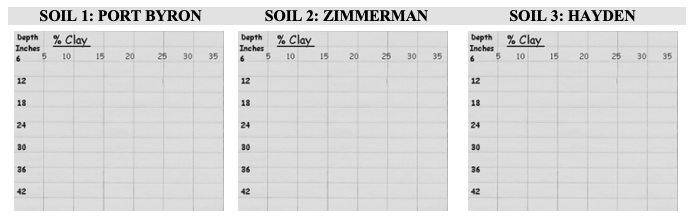
\includegraphics{clay-eluviation-illuviation-graph.png}

All three of these soils developed under a similar climate in
central-eastern Minnesota. The Zimmerman soil is formed in outwash under
forest vegetation. The Port Byron soil is formed in loess under
grassland vegetation. The Hayden soil is formed in glacial till under
forest vegetation. REMEMBER: Soils developed under grasslands typically
have more organic matter and organic matter is an excellent binding
agent of mineral particles (remember the pictures of granular structure
and the clay particles bound by OM).

\begin{enumerate}
\def\labelenumi{\arabic{enumi}.}
\tightlist
\item
  Which of these soils exhibits a clear peak in clay with depth?
\end{enumerate}

~ ~ ~

\begin{enumerate}
\def\labelenumi{\arabic{enumi}.}
\setcounter{enumi}{1}
\tightlist
\item
  Knowing what you know about the soil forming factors and their effect
  on soil development and soil morphology, explain why the soil listed
  in your answer to question 1 has a peak in clay due to
  eluviation/illuviation while the other soils do not.
\end{enumerate}

~ ~ ~

\hypertarget{investigation-h-properties-from-factors-and-factors-from-properties}{%
\section{INVESTIGATION H: Properties from Factors and Factors from
Properties}\label{investigation-h-properties-from-factors-and-factors-from-properties}}

Some knowledge of soil forming factors at work on a particular landscape
or in the formation of a particular soil allow us to predict soil
properties such as horizon morphology, texture, color, organic matter,
and mineralogy. Below, complete the tables with the choices given on the
handout (use each only once) based on your knowledge from class. Use the
information on both the ``Soil Forming Factors'' and ``Soil Properties''
tables to fill in the blanks. All of the information you need should be
present in these tables, however, you can use the monoliths in the
display area to help you with your choices if that helps you to better
visualize the soils.

 
  \providecommand{\huxb}[2]{\arrayrulecolor[RGB]{#1}\global\arrayrulewidth=#2pt}
  \providecommand{\huxvb}[2]{\color[RGB]{#1}\vrule width #2pt}
  \providecommand{\huxtpad}[1]{\rule{0pt}{#1}}
  \providecommand{\huxbpad}[1]{\rule[-#1]{0pt}{#1}}

\begin{table}[h!]
\begin{centerbox}
\begin{threeparttable}
 
\setlength{\tabcolsep}{0pt}
\begin{tabularx}{0.9\textwidth}{p{0.15\textwidth} p{0.15\textwidth} p{0.15\textwidth} p{0.15\textwidth} p{0.15\textwidth} p{0.15\textwidth}}


\hhline{>{\huxb{0, 0, 0}{1}}->{\huxb{0, 0, 0}{1}}->{\huxb{0, 0, 0}{1}}->{\huxb{0, 0, 0}{1}}->{\huxb{0, 0, 0}{1}}->{\huxb{0, 0, 0}{1}}-}
\arrayrulecolor{black}

\multicolumn{1}{!{\huxvb{0, 0, 0}{1}}m{0.15\textwidth}!{\huxvb{0, 0, 0}{1}}}{\hspace{0pt}\parbox[c]{0.15\textwidth-0pt-4pt}{\huxtpad{0pt + 1em}\centering \textbf{Soil Series Name}\huxbpad{4pt}}} &
\multicolumn{1}{m{0.15\textwidth}!{\huxvb{0, 0, 0}{1}}}{\hspace{4pt}\parbox[c]{0.15\textwidth-4pt-4pt}{\huxtpad{0pt + 1em}\centering \textbf{Parent Material}\huxbpad{4pt}}} &
\multicolumn{1}{m{0.15\textwidth}!{\huxvb{0, 0, 0}{1}}}{\hspace{4pt}\parbox[c]{0.15\textwidth-4pt-4pt}{\huxtpad{0pt + 1em}\centering \textbf{Climate}\huxbpad{4pt}}} &
\multicolumn{1}{m{0.15\textwidth}!{\huxvb{0, 0, 0}{1}}}{\hspace{4pt}\parbox[c]{0.15\textwidth-4pt-4pt}{\huxtpad{0pt + 1em}\centering \textbf{Organisms (Vegetation)}\huxbpad{4pt}}} &
\multicolumn{1}{m{0.15\textwidth}!{\huxvb{0, 0, 0}{1}}}{\hspace{4pt}\parbox[c]{0.15\textwidth-4pt-4pt}{\huxtpad{0pt + 1em}\centering \textbf{Relief (Hillslope Position)}\huxbpad{4pt}}} &
\multicolumn{1}{m{0.15\textwidth}!{\huxvb{0, 0, 0}{1}}}{\hspace{4pt}\parbox[c]{0.15\textwidth-4pt-0pt}{\huxtpad{0pt + 1em}\centering \textbf{Time}\huxbpad{4pt}}} \tabularnewline[-0.5pt]


\hhline{>{\huxb{0, 0, 0}{1}}->{\huxb{0, 0, 0}{1}}->{\huxb{0, 0, 0}{1}}->{\huxb{0, 0, 0}{1}}->{\huxb{0, 0, 0}{1}}->{\huxb{0, 0, 0}{1}}-}
\arrayrulecolor{black}

\multicolumn{1}{!{\huxvb{0, 0, 0}{1}}m{0.15\textwidth}!{\huxvb{0, 0, 0}{1}}}{\hspace{0pt}\parbox[c]{0.15\textwidth-0pt-4pt}{\huxtpad{4pt + 1em}\centering Hayden\huxbpad{4pt}}} &
\multicolumn{1}{m{0.15\textwidth}!{\huxvb{0, 0, 0}{1}}}{\hspace{4pt}\parbox[c]{0.15\textwidth-4pt-4pt}{\huxtpad{4pt + 1em}\centering Des Moines Lobe Till\huxbpad{4pt}}} &
\multicolumn{1}{m{0.15\textwidth}!{\huxvb{0, 0, 0}{1}}}{\hspace{4pt}\parbox[c]{0.15\textwidth-4pt-4pt}{\huxtpad{4pt + 1em}\centering Humid Temperate\huxbpad{4pt}}} &
\multicolumn{1}{m{0.15\textwidth}!{\huxvb{0, 0, 0}{1}}}{\hspace{4pt}\parbox[c]{0.15\textwidth-4pt-4pt}{\huxtpad{4pt + 1em}\centering Forest\huxbpad{4pt}}} &
\multicolumn{1}{m{0.15\textwidth}!{\huxvb{0, 0, 0}{1}}}{\hspace{4pt}\parbox[c]{0.15\textwidth-4pt-4pt}{\huxtpad{4pt + 1em}\centering Summit/Shoulder\huxbpad{4pt}}} &
\multicolumn{1}{m{0.15\textwidth}!{\huxvb{0, 0, 0}{1}}}{\hspace{4pt}\parbox[c]{0.15\textwidth-4pt-0pt}{\huxtpad{4pt + 1em}\centering \~{}10,0 years\huxbpad{4pt}}} \tabularnewline[-0.5pt]


\hhline{>{\huxb{0, 0, 0}{1}}->{\huxb{0, 0, 0}{1}}->{\huxb{0, 0, 0}{1}}->{\huxb{0, 0, 0}{1}}->{\huxb{0, 0, 0}{1}}->{\huxb{0, 0, 0}{1}}-}
\arrayrulecolor{black}

\multicolumn{1}{!{\huxvb{0, 0, 0}{1}}m{0.15\textwidth}!{\huxvb{0, 0, 0}{1}}}{\hspace{0pt}\parbox[c]{0.15\textwidth-0pt-4pt}{\huxtpad{4pt + 1em}\centering Port Byron\huxbpad{4pt}}} &
\multicolumn{1}{m{0.15\textwidth}!{\huxvb{0, 0, 0}{1}}}{\hspace{4pt}\parbox[c]{0.15\textwidth-4pt-4pt}{\huxtpad{4pt + 1em}\centering \huxbpad{4pt}}} &
\multicolumn{1}{m{0.15\textwidth}!{\huxvb{0, 0, 0}{1}}}{\hspace{4pt}\parbox[c]{0.15\textwidth-4pt-4pt}{\huxtpad{4pt + 1em}\centering Humid Temperate\huxbpad{4pt}}} &
\multicolumn{1}{m{0.15\textwidth}!{\huxvb{0, 0, 0}{1}}}{\hspace{4pt}\parbox[c]{0.15\textwidth-4pt-4pt}{\huxtpad{4pt + 1em}\centering \huxbpad{4pt}}} &
\multicolumn{1}{m{0.15\textwidth}!{\huxvb{0, 0, 0}{1}}}{\hspace{4pt}\parbox[c]{0.15\textwidth-4pt-4pt}{\huxtpad{4pt + 1em}\centering Summit/Shoulder\huxbpad{4pt}}} &
\multicolumn{1}{m{0.15\textwidth}!{\huxvb{0, 0, 0}{1}}}{\hspace{4pt}\parbox[c]{0.15\textwidth-4pt-0pt}{\huxtpad{4pt + 1em}\centering \~{}10,0 years\huxbpad{4pt}}} \tabularnewline[-0.5pt]


\hhline{>{\huxb{0, 0, 0}{1}}->{\huxb{0, 0, 0}{1}}->{\huxb{0, 0, 0}{1}}->{\huxb{0, 0, 0}{1}}->{\huxb{0, 0, 0}{1}}->{\huxb{0, 0, 0}{1}}-}
\arrayrulecolor{black}

\multicolumn{1}{!{\huxvb{0, 0, 0}{1}}m{0.15\textwidth}!{\huxvb{0, 0, 0}{1}}}{\hspace{0pt}\parbox[c]{0.15\textwidth-0pt-4pt}{\huxtpad{4pt + 1em}\centering Zimmerman\huxbpad{4pt}}} &
\multicolumn{1}{m{0.15\textwidth}!{\huxvb{0, 0, 0}{1}}}{\hspace{4pt}\parbox[c]{0.15\textwidth-4pt-4pt}{\huxtpad{4pt + 1em}\centering \huxbpad{4pt}}} &
\multicolumn{1}{m{0.15\textwidth}!{\huxvb{0, 0, 0}{1}}}{\hspace{4pt}\parbox[c]{0.15\textwidth-4pt-4pt}{\huxtpad{4pt + 1em}\centering Humid Temperate\huxbpad{4pt}}} &
\multicolumn{1}{m{0.15\textwidth}!{\huxvb{0, 0, 0}{1}}}{\hspace{4pt}\parbox[c]{0.15\textwidth-4pt-4pt}{\huxtpad{4pt + 1em}\centering Forest\huxbpad{4pt}}} &
\multicolumn{1}{m{0.15\textwidth}!{\huxvb{0, 0, 0}{1}}}{\hspace{4pt}\parbox[c]{0.15\textwidth-4pt-4pt}{\huxtpad{4pt + 1em}\centering Summit/Shoulder\huxbpad{4pt}}} &
\multicolumn{1}{m{0.15\textwidth}!{\huxvb{0, 0, 0}{1}}}{\hspace{4pt}\parbox[c]{0.15\textwidth-4pt-0pt}{\huxtpad{4pt + 1em}\centering \~{}10,0 years\huxbpad{4pt}}} \tabularnewline[-0.5pt]


\hhline{>{\huxb{0, 0, 0}{1}}->{\huxb{0, 0, 0}{1}}->{\huxb{0, 0, 0}{1}}->{\huxb{0, 0, 0}{1}}->{\huxb{0, 0, 0}{1}}->{\huxb{0, 0, 0}{1}}-}
\arrayrulecolor{black}

\multicolumn{1}{!{\huxvb{0, 0, 0}{1}}m{0.15\textwidth}!{\huxvb{0, 0, 0}{1}}}{\hspace{0pt}\parbox[c]{0.15\textwidth-0pt-4pt}{\huxtpad{4pt + 1em}\centering Cecil\huxbpad{4pt}}} &
\multicolumn{1}{m{0.15\textwidth}!{\huxvb{0, 0, 0}{1}}}{\hspace{4pt}\parbox[c]{0.15\textwidth-4pt-4pt}{\huxtpad{4pt + 1em}\centering Igneous/Metamorphic Residuum\huxbpad{4pt}}} &
\multicolumn{1}{m{0.15\textwidth}!{\huxvb{0, 0, 0}{1}}}{\hspace{4pt}\parbox[c]{0.15\textwidth-4pt-4pt}{\huxtpad{4pt + 1em}\centering Humid Subtropical\huxbpad{4pt}}} &
\multicolumn{1}{m{0.15\textwidth}!{\huxvb{0, 0, 0}{1}}}{\hspace{4pt}\parbox[c]{0.15\textwidth-4pt-4pt}{\huxtpad{4pt + 1em}\centering \huxbpad{4pt}}} &
\multicolumn{1}{m{0.15\textwidth}!{\huxvb{0, 0, 0}{1}}}{\hspace{4pt}\parbox[c]{0.15\textwidth-4pt-4pt}{\huxtpad{4pt + 1em}\centering Summit/Shoulder\huxbpad{4pt}}} &
\multicolumn{1}{m{0.15\textwidth}!{\huxvb{0, 0, 0}{1}}}{\hspace{4pt}\parbox[c]{0.15\textwidth-4pt-0pt}{\huxtpad{4pt + 1em}\centering \~{}200,0 years\huxbpad{4pt}}} \tabularnewline[-0.5pt]


\hhline{>{\huxb{0, 0, 0}{1}}->{\huxb{0, 0, 0}{1}}->{\huxb{0, 0, 0}{1}}->{\huxb{0, 0, 0}{1}}->{\huxb{0, 0, 0}{1}}->{\huxb{0, 0, 0}{1}}-}
\arrayrulecolor{black}

\multicolumn{1}{!{\huxvb{0, 0, 0}{1}}m{0.15\textwidth}!{\huxvb{0, 0, 0}{1}}}{\hspace{0pt}\parbox[c]{0.15\textwidth-0pt-4pt}{\huxtpad{4pt + 1em}\centering Rifle\huxbpad{4pt}}} &
\multicolumn{1}{m{0.15\textwidth}!{\huxvb{0, 0, 0}{1}}}{\hspace{4pt}\parbox[c]{0.15\textwidth-4pt-4pt}{\huxtpad{4pt + 1em}\centering Organic Deposits\huxbpad{4pt}}} &
\multicolumn{1}{m{0.15\textwidth}!{\huxvb{0, 0, 0}{1}}}{\hspace{4pt}\parbox[c]{0.15\textwidth-4pt-4pt}{\huxtpad{4pt + 1em}\centering \huxbpad{4pt}}} &
\multicolumn{1}{m{0.15\textwidth}!{\huxvb{0, 0, 0}{1}}}{\hspace{4pt}\parbox[c]{0.15\textwidth-4pt-4pt}{\huxtpad{4pt + 1em}\centering Wetland\huxbpad{4pt}}} &
\multicolumn{1}{m{0.15\textwidth}!{\huxvb{0, 0, 0}{1}}}{\hspace{4pt}\parbox[c]{0.15\textwidth-4pt-4pt}{\huxtpad{4pt + 1em}\centering Toeslope\huxbpad{4pt}}} &
\multicolumn{1}{m{0.15\textwidth}!{\huxvb{0, 0, 0}{1}}}{\hspace{4pt}\parbox[c]{0.15\textwidth-4pt-0pt}{\huxtpad{4pt + 1em}\centering \~{}10,0 years\huxbpad{4pt}}} \tabularnewline[-0.5pt]


\hhline{>{\huxb{0, 0, 0}{1}}->{\huxb{0, 0, 0}{1}}->{\huxb{0, 0, 0}{1}}->{\huxb{0, 0, 0}{1}}->{\huxb{0, 0, 0}{1}}->{\huxb{0, 0, 0}{1}}-}
\arrayrulecolor{black}

\multicolumn{1}{!{\huxvb{0, 0, 0}{1}}m{0.15\textwidth}!{\huxvb{0, 0, 0}{1}}}{\hspace{0pt}\parbox[c]{0.15\textwidth-0pt-4pt}{\huxtpad{4pt + 1em}\centering Balaton\huxbpad{4pt}}} &
\multicolumn{1}{m{0.15\textwidth}!{\huxvb{0, 0, 0}{1}}}{\hspace{4pt}\parbox[c]{0.15\textwidth-4pt-4pt}{\huxtpad{4pt + 1em}\centering Des Moines Lobe Till\huxbpad{4pt}}} &
\multicolumn{1}{m{0.15\textwidth}!{\huxvb{0, 0, 0}{1}}}{\hspace{4pt}\parbox[c]{0.15\textwidth-4pt-4pt}{\huxtpad{4pt + 1em}\centering \huxbpad{4pt}}} &
\multicolumn{1}{m{0.15\textwidth}!{\huxvb{0, 0, 0}{1}}}{\hspace{4pt}\parbox[c]{0.15\textwidth-4pt-4pt}{\huxtpad{4pt + 1em}\centering Grassland\huxbpad{4pt}}} &
\multicolumn{1}{m{0.15\textwidth}!{\huxvb{0, 0, 0}{1}}}{\hspace{4pt}\parbox[c]{0.15\textwidth-4pt-4pt}{\huxtpad{4pt + 1em}\centering Summit\huxbpad{4pt}}} &
\multicolumn{1}{m{0.15\textwidth}!{\huxvb{0, 0, 0}{1}}}{\hspace{4pt}\parbox[c]{0.15\textwidth-4pt-0pt}{\huxtpad{4pt + 1em}\centering \~{}10,0 years\huxbpad{4pt}}} \tabularnewline[-0.5pt]


\hhline{>{\huxb{0, 0, 0}{1}}->{\huxb{0, 0, 0}{1}}->{\huxb{0, 0, 0}{1}}->{\huxb{0, 0, 0}{1}}->{\huxb{0, 0, 0}{1}}->{\huxb{0, 0, 0}{1}}-}
\arrayrulecolor{black}

\multicolumn{1}{!{\huxvb{0, 0, 0}{1}}m{0.15\textwidth}!{\huxvb{0, 0, 0}{1}}}{\hspace{0pt}\parbox[c]{0.15\textwidth-0pt-4pt}{\huxtpad{4pt + 1em}\centering Kingsley\huxbpad{0pt}}} &
\multicolumn{1}{m{0.15\textwidth}!{\huxvb{0, 0, 0}{1}}}{\hspace{4pt}\parbox[c]{0.15\textwidth-4pt-4pt}{\huxtpad{4pt + 1em}\centering Superior Lobe Till\huxbpad{0pt}}} &
\multicolumn{1}{m{0.15\textwidth}!{\huxvb{0, 0, 0}{1}}}{\hspace{4pt}\parbox[c]{0.15\textwidth-4pt-4pt}{\huxtpad{4pt + 1em}\centering Humid Temperate\huxbpad{0pt}}} &
\multicolumn{1}{m{0.15\textwidth}!{\huxvb{0, 0, 0}{1}}}{\hspace{4pt}\parbox[c]{0.15\textwidth-4pt-4pt}{\huxtpad{4pt + 1em}\centering Forest\huxbpad{0pt}}} &
\multicolumn{1}{m{0.15\textwidth}!{\huxvb{0, 0, 0}{1}}}{\hspace{4pt}\parbox[c]{0.15\textwidth-4pt-4pt}{\huxtpad{4pt + 1em}\centering Summit/Shoulder\huxbpad{0pt}}} &
\multicolumn{1}{m{0.15\textwidth}!{\huxvb{0, 0, 0}{1}}}{\hspace{4pt}\parbox[c]{0.15\textwidth-4pt-0pt}{\huxtpad{4pt + 1em}\centering \~{}10,0 years\huxbpad{0pt}}} \tabularnewline[-0.5pt]


\hhline{>{\huxb{0, 0, 0}{1}}->{\huxb{0, 0, 0}{1}}->{\huxb{0, 0, 0}{1}}->{\huxb{0, 0, 0}{1}}->{\huxb{0, 0, 0}{1}}->{\huxb{0, 0, 0}{1}}-}
\arrayrulecolor{black}
\end{tabularx}
\end{threeparttable}\par\end{centerbox}

\end{table}
 

 
  \providecommand{\huxb}[2]{\arrayrulecolor[RGB]{#1}\global\arrayrulewidth=#2pt}
  \providecommand{\huxvb}[2]{\color[RGB]{#1}\vrule width #2pt}
  \providecommand{\huxtpad}[1]{\rule{0pt}{#1}}
  \providecommand{\huxbpad}[1]{\rule[-#1]{0pt}{#1}}

\begin{table}[h!]
\begin{centerbox}
\begin{threeparttable}
 
\setlength{\tabcolsep}{0pt}
\begin{tabularx}{0.9\textwidth}{p{0.128571428571429\textwidth} p{0.128571428571429\textwidth} p{0.128571428571429\textwidth} p{0.128571428571429\textwidth} p{0.128571428571429\textwidth} p{0.128571428571429\textwidth} p{0.128571428571429\textwidth}}


\hhline{>{\huxb{0, 0, 0}{1}}->{\huxb{0, 0, 0}{1}}->{\huxb{0, 0, 0}{1}}->{\huxb{0, 0, 0}{1}}->{\huxb{0, 0, 0}{1}}->{\huxb{0, 0, 0}{1}}->{\huxb{0, 0, 0}{1}}-}
\arrayrulecolor{black}

\multicolumn{1}{!{\huxvb{0, 0, 0}{1}}m{0.128571428571429\textwidth}!{\huxvb{0, 0, 0}{1}}}{\hspace{0pt}\parbox[c]{0.128571428571429\textwidth-0pt-4pt}{\huxtpad{0pt + 1em}\centering \textbf{Soil Series Name}\huxbpad{4pt}}} &
\multicolumn{1}{m{0.128571428571429\textwidth}!{\huxvb{0, 0, 0}{1}}}{\hspace{4pt}\parbox[c]{0.128571428571429\textwidth-4pt-4pt}{\huxtpad{0pt + 1em}\centering \textbf{Dominant Texture}\huxbpad{4pt}}} &
\multicolumn{1}{m{0.128571428571429\textwidth}!{\huxvb{0, 0, 0}{1}}}{\hspace{4pt}\parbox[c]{0.128571428571429\textwidth-4pt-4pt}{\huxtpad{0pt + 1em}\centering \textbf{Subsoil Color}\huxbpad{4pt}}} &
\multicolumn{1}{m{0.128571428571429\textwidth}!{\huxvb{0, 0, 0}{1}}}{\hspace{4pt}\parbox[c]{0.128571428571429\textwidth-4pt-4pt}{\huxtpad{0pt + 1em}\centering \textbf{Drainage Class}\huxbpad{4pt}}} &
\multicolumn{1}{m{0.128571428571429\textwidth}!{\huxvb{0, 0, 0}{1}}}{\hspace{4pt}\parbox[c]{0.128571428571429\textwidth-4pt-4pt}{\huxtpad{0pt + 1em}\centering \textbf{Topsoil Organic Matter Content (\%)}\huxbpad{4pt}}} &
\multicolumn{1}{m{0.128571428571429\textwidth}!{\huxvb{0, 0, 0}{1}}}{\hspace{4pt}\parbox[c]{0.128571428571429\textwidth-4pt-4pt}{\huxtpad{0pt + 1em}\centering \textbf{Mineralogy}\huxbpad{4pt}}} &
\multicolumn{1}{m{0.128571428571429\textwidth}!{\huxvb{0, 0, 0}{1}}}{\hspace{4pt}\parbox[c]{0.128571428571429\textwidth-4pt-0pt}{\huxtpad{0pt + 1em}\centering \textbf{Coarse Fragments}\huxbpad{4pt}}} \tabularnewline[-0.5pt]


\hhline{>{\huxb{0, 0, 0}{1}}->{\huxb{0, 0, 0}{1}}->{\huxb{0, 0, 0}{1}}->{\huxb{0, 0, 0}{1}}->{\huxb{0, 0, 0}{1}}->{\huxb{0, 0, 0}{1}}->{\huxb{0, 0, 0}{1}}-}
\arrayrulecolor{black}

\multicolumn{1}{!{\huxvb{0, 0, 0}{1}}m{0.128571428571429\textwidth}!{\huxvb{0, 0, 0}{1}}}{\hspace{0pt}\parbox[c]{0.128571428571429\textwidth-0pt-4pt}{\huxtpad{4pt + 1em}\centering Hayden\huxbpad{4pt}}} &
\multicolumn{1}{m{0.128571428571429\textwidth}!{\huxvb{0, 0, 0}{1}}}{\hspace{4pt}\parbox[c]{0.128571428571429\textwidth-4pt-4pt}{\huxtpad{4pt + 1em}\centering Clay Loam/Silty Clay Loam\huxbpad{4pt}}} &
\multicolumn{1}{m{0.128571428571429\textwidth}!{\huxvb{0, 0, 0}{1}}}{\hspace{4pt}\parbox[c]{0.128571428571429\textwidth-4pt-4pt}{\huxtpad{4pt + 1em}\centering 2Y\huxbpad{4pt}}} &
\multicolumn{1}{m{0.128571428571429\textwidth}!{\huxvb{0, 0, 0}{1}}}{\hspace{4pt}\parbox[c]{0.128571428571429\textwidth-4pt-4pt}{\huxtpad{4pt + 1em}\centering Well Drained\huxbpad{4pt}}} &
\multicolumn{1}{m{0.128571428571429\textwidth}!{\huxvb{0, 0, 0}{1}}}{\hspace{4pt}\parbox[c]{0.128571428571429\textwidth-4pt-4pt}{\huxtpad{4pt + 1em}\centering \huxbpad{4pt}}} &
\multicolumn{1}{m{0.128571428571429\textwidth}!{\huxvb{0, 0, 0}{1}}}{\hspace{4pt}\parbox[c]{0.128571428571429\textwidth-4pt-4pt}{\huxtpad{4pt + 1em}\centering Illites/Smec./Verm.\huxbpad{4pt}}} &
\multicolumn{1}{m{0.128571428571429\textwidth}!{\huxvb{0, 0, 0}{1}}}{\hspace{4pt}\parbox[c]{0.128571428571429\textwidth-4pt-0pt}{\huxtpad{4pt + 1em}\centering Y\huxbpad{4pt}}} \tabularnewline[-0.5pt]


\hhline{>{\huxb{0, 0, 0}{1}}->{\huxb{0, 0, 0}{1}}->{\huxb{0, 0, 0}{1}}->{\huxb{0, 0, 0}{1}}->{\huxb{0, 0, 0}{1}}->{\huxb{0, 0, 0}{1}}->{\huxb{0, 0, 0}{1}}-}
\arrayrulecolor{black}

\multicolumn{1}{!{\huxvb{0, 0, 0}{1}}m{0.128571428571429\textwidth}!{\huxvb{0, 0, 0}{1}}}{\hspace{0pt}\parbox[c]{0.128571428571429\textwidth-0pt-4pt}{\huxtpad{4pt + 1em}\centering Port Byron\huxbpad{4pt}}} &
\multicolumn{1}{m{0.128571428571429\textwidth}!{\huxvb{0, 0, 0}{1}}}{\hspace{4pt}\parbox[c]{0.128571428571429\textwidth-4pt-4pt}{\huxtpad{4pt + 1em}\centering Silt/Silt Loam\huxbpad{4pt}}} &
\multicolumn{1}{m{0.128571428571429\textwidth}!{\huxvb{0, 0, 0}{1}}}{\hspace{4pt}\parbox[c]{0.128571428571429\textwidth-4pt-4pt}{\huxtpad{4pt + 1em}\centering 10YR\huxbpad{4pt}}} &
\multicolumn{1}{m{0.128571428571429\textwidth}!{\huxvb{0, 0, 0}{1}}}{\hspace{4pt}\parbox[c]{0.128571428571429\textwidth-4pt-4pt}{\huxtpad{4pt + 1em}\centering \huxbpad{4pt}}} &
\multicolumn{1}{m{0.128571428571429\textwidth}!{\huxvb{0, 0, 0}{1}}}{\hspace{4pt}\parbox[c]{0.128571428571429\textwidth-4pt-4pt}{\huxtpad{4pt + 1em}\centering 10\%\huxbpad{4pt}}} &
\multicolumn{1}{m{0.128571428571429\textwidth}!{\huxvb{0, 0, 0}{1}}}{\hspace{4pt}\parbox[c]{0.128571428571429\textwidth-4pt-4pt}{\huxtpad{4pt + 1em}\centering Illites/Smec./Verm.\huxbpad{4pt}}} &
\multicolumn{1}{m{0.128571428571429\textwidth}!{\huxvb{0, 0, 0}{1}}}{\hspace{4pt}\parbox[c]{0.128571428571429\textwidth-4pt-0pt}{\huxtpad{4pt + 1em}\centering N\huxbpad{4pt}}} \tabularnewline[-0.5pt]


\hhline{>{\huxb{0, 0, 0}{1}}->{\huxb{0, 0, 0}{1}}->{\huxb{0, 0, 0}{1}}->{\huxb{0, 0, 0}{1}}->{\huxb{0, 0, 0}{1}}->{\huxb{0, 0, 0}{1}}->{\huxb{0, 0, 0}{1}}-}
\arrayrulecolor{black}

\multicolumn{1}{!{\huxvb{0, 0, 0}{1}}m{0.128571428571429\textwidth}!{\huxvb{0, 0, 0}{1}}}{\hspace{0pt}\parbox[c]{0.128571428571429\textwidth-0pt-4pt}{\huxtpad{4pt + 1em}\centering Zimmerman\huxbpad{4pt}}} &
\multicolumn{1}{m{0.128571428571429\textwidth}!{\huxvb{0, 0, 0}{1}}}{\hspace{4pt}\parbox[c]{0.128571428571429\textwidth-4pt-4pt}{\huxtpad{4pt + 1em}\centering Sand/Loamy Sand\huxbpad{4pt}}} &
\multicolumn{1}{m{0.128571428571429\textwidth}!{\huxvb{0, 0, 0}{1}}}{\hspace{4pt}\parbox[c]{0.128571428571429\textwidth-4pt-4pt}{\huxtpad{4pt + 1em}\centering 10YR\huxbpad{4pt}}} &
\multicolumn{1}{m{0.128571428571429\textwidth}!{\huxvb{0, 0, 0}{1}}}{\hspace{4pt}\parbox[c]{0.128571428571429\textwidth-4pt-4pt}{\huxtpad{4pt + 1em}\centering Well Drained\huxbpad{4pt}}} &
\multicolumn{1}{m{0.128571428571429\textwidth}!{\huxvb{0, 0, 0}{1}}}{\hspace{4pt}\parbox[c]{0.128571428571429\textwidth-4pt-4pt}{\huxtpad{4pt + 1em}\centering 5\%\huxbpad{4pt}}} &
\multicolumn{1}{m{0.128571428571429\textwidth}!{\huxvb{0, 0, 0}{1}}}{\hspace{4pt}\parbox[c]{0.128571428571429\textwidth-4pt-4pt}{\huxtpad{4pt + 1em}\centering Quartz\huxbpad{4pt}}} &
\multicolumn{1}{m{0.128571428571429\textwidth}!{\huxvb{0, 0, 0}{1}}}{\hspace{4pt}\parbox[c]{0.128571428571429\textwidth-4pt-0pt}{\huxtpad{4pt + 1em}\centering Y\huxbpad{4pt}}} \tabularnewline[-0.5pt]


\hhline{>{\huxb{0, 0, 0}{1}}->{\huxb{0, 0, 0}{1}}->{\huxb{0, 0, 0}{1}}->{\huxb{0, 0, 0}{1}}->{\huxb{0, 0, 0}{1}}->{\huxb{0, 0, 0}{1}}->{\huxb{0, 0, 0}{1}}-}
\arrayrulecolor{black}

\multicolumn{1}{!{\huxvb{0, 0, 0}{1}}m{0.128571428571429\textwidth}!{\huxvb{0, 0, 0}{1}}}{\hspace{0pt}\parbox[c]{0.128571428571429\textwidth-0pt-4pt}{\huxtpad{4pt + 1em}\centering Cecil\huxbpad{4pt}}} &
\multicolumn{1}{m{0.128571428571429\textwidth}!{\huxvb{0, 0, 0}{1}}}{\hspace{4pt}\parbox[c]{0.128571428571429\textwidth-4pt-4pt}{\huxtpad{4pt + 1em}\centering Clay Loam/Clay\huxbpad{4pt}}} &
\multicolumn{1}{m{0.128571428571429\textwidth}!{\huxvb{0, 0, 0}{1}}}{\hspace{4pt}\parbox[c]{0.128571428571429\textwidth-4pt-4pt}{\huxtpad{4pt + 1em}\centering 2R\huxbpad{4pt}}} &
\multicolumn{1}{m{0.128571428571429\textwidth}!{\huxvb{0, 0, 0}{1}}}{\hspace{4pt}\parbox[c]{0.128571428571429\textwidth-4pt-4pt}{\huxtpad{4pt + 1em}\centering Well Drained\huxbpad{4pt}}} &
\multicolumn{1}{m{0.128571428571429\textwidth}!{\huxvb{0, 0, 0}{1}}}{\hspace{4pt}\parbox[c]{0.128571428571429\textwidth-4pt-4pt}{\huxtpad{4pt + 1em}\centering 5\%\huxbpad{4pt}}} &
\multicolumn{1}{m{0.128571428571429\textwidth}!{\huxvb{0, 0, 0}{1}}}{\hspace{4pt}\parbox[c]{0.128571428571429\textwidth-4pt-4pt}{\huxtpad{4pt + 1em}\centering \huxbpad{4pt}}} &
\multicolumn{1}{m{0.128571428571429\textwidth}!{\huxvb{0, 0, 0}{1}}}{\hspace{4pt}\parbox[c]{0.128571428571429\textwidth-4pt-0pt}{\huxtpad{4pt + 1em}\centering N\huxbpad{4pt}}} \tabularnewline[-0.5pt]


\hhline{>{\huxb{0, 0, 0}{1}}->{\huxb{0, 0, 0}{1}}->{\huxb{0, 0, 0}{1}}->{\huxb{0, 0, 0}{1}}->{\huxb{0, 0, 0}{1}}->{\huxb{0, 0, 0}{1}}->{\huxb{0, 0, 0}{1}}-}
\arrayrulecolor{black}

\multicolumn{1}{!{\huxvb{0, 0, 0}{1}}m{0.128571428571429\textwidth}!{\huxvb{0, 0, 0}{1}}}{\hspace{0pt}\parbox[c]{0.128571428571429\textwidth-0pt-4pt}{\huxtpad{4pt + 1em}\centering Rifle\huxbpad{20pt}}} &
\multicolumn{1}{m{0.128571428571429\textwidth}!{\huxvb{0, 0, 0}{1}}}{\hspace{4pt}\parbox[c]{0.128571428571429\textwidth-4pt-4pt}{\huxtpad{4pt + 1em}\centering N/A\huxbpad{20pt}}} &
\multicolumn{1}{m{0.128571428571429\textwidth}!{\huxvb{0, 0, 0}{1}}}{\hspace{4pt}\parbox[c]{0.128571428571429\textwidth-4pt-4pt}{\huxtpad{4pt + 1em}\centering 10YR\huxbpad{20pt}}} &
\multicolumn{1}{m{0.128571428571429\textwidth}!{\huxvb{0, 0, 0}{1}}}{\hspace{4pt}\parbox[c]{0.128571428571429\textwidth-4pt-4pt}{\huxtpad{4pt + 1em}\centering \huxbpad{20pt}}} &
\multicolumn{1}{m{0.128571428571429\textwidth}!{\huxvb{0, 0, 0}{1}}}{\hspace{4pt}\parbox[c]{0.128571428571429\textwidth-4pt-4pt}{\huxtpad{4pt + 1em}\centering \huxbpad{20pt}}} &
\multicolumn{1}{m{0.128571428571429\textwidth}!{\huxvb{0, 0, 0}{1}}}{\hspace{4pt}\parbox[c]{0.128571428571429\textwidth-4pt-4pt}{\huxtpad{4pt + 1em}\centering N/A\huxbpad{20pt}}} &
\multicolumn{1}{m{0.128571428571429\textwidth}!{\huxvb{0, 0, 0}{1}}}{\hspace{4pt}\parbox[c]{0.128571428571429\textwidth-4pt-0pt}{\huxtpad{4pt + 1em}\centering N\huxbpad{20pt}}} \tabularnewline[-0.5pt]


\hhline{>{\huxb{0, 0, 0}{1}}->{\huxb{0, 0, 0}{1}}->{\huxb{0, 0, 0}{1}}->{\huxb{0, 0, 0}{1}}->{\huxb{0, 0, 0}{1}}->{\huxb{0, 0, 0}{1}}->{\huxb{0, 0, 0}{1}}-}
\arrayrulecolor{black}

\multicolumn{1}{!{\huxvb{0, 0, 0}{1}}m{0.128571428571429\textwidth}!{\huxvb{0, 0, 0}{1}}}{\hspace{0pt}\parbox[c]{0.128571428571429\textwidth-0pt-4pt}{\huxtpad{4pt + 1em}\centering Balaton\huxbpad{4pt}}} &
\multicolumn{1}{m{0.128571428571429\textwidth}!{\huxvb{0, 0, 0}{1}}}{\hspace{4pt}\parbox[c]{0.128571428571429\textwidth-4pt-4pt}{\huxtpad{4pt + 1em}\centering Clay Loam/Silty Clay Loam\huxbpad{4pt}}} &
\multicolumn{1}{m{0.128571428571429\textwidth}!{\huxvb{0, 0, 0}{1}}}{\hspace{4pt}\parbox[c]{0.128571428571429\textwidth-4pt-4pt}{\huxtpad{4pt + 1em}\centering \huxbpad{4pt}}} &
\multicolumn{1}{m{0.128571428571429\textwidth}!{\huxvb{0, 0, 0}{1}}}{\hspace{4pt}\parbox[c]{0.128571428571429\textwidth-4pt-4pt}{\huxtpad{4pt + 1em}\centering Well Drained\huxbpad{4pt}}} &
\multicolumn{1}{m{0.128571428571429\textwidth}!{\huxvb{0, 0, 0}{1}}}{\hspace{4pt}\parbox[c]{0.128571428571429\textwidth-4pt-4pt}{\huxtpad{4pt + 1em}\centering 10\%\huxbpad{4pt}}} &
\multicolumn{1}{m{0.128571428571429\textwidth}!{\huxvb{0, 0, 0}{1}}}{\hspace{4pt}\parbox[c]{0.128571428571429\textwidth-4pt-4pt}{\huxtpad{4pt + 1em}\centering \huxbpad{4pt}}} &
\multicolumn{1}{m{0.128571428571429\textwidth}!{\huxvb{0, 0, 0}{1}}}{\hspace{4pt}\parbox[c]{0.128571428571429\textwidth-4pt-0pt}{\huxtpad{4pt + 1em}\centering Y\huxbpad{4pt}}} \tabularnewline[-0.5pt]


\hhline{>{\huxb{0, 0, 0}{1}}->{\huxb{0, 0, 0}{1}}->{\huxb{0, 0, 0}{1}}->{\huxb{0, 0, 0}{1}}->{\huxb{0, 0, 0}{1}}->{\huxb{0, 0, 0}{1}}->{\huxb{0, 0, 0}{1}}-}
\arrayrulecolor{black}

\multicolumn{1}{!{\huxvb{0, 0, 0}{1}}m{0.128571428571429\textwidth}!{\huxvb{0, 0, 0}{1}}}{\hspace{0pt}\parbox[c]{0.128571428571429\textwidth-0pt-4pt}{\huxtpad{4pt + 1em}\centering Kingsley\huxbpad{0pt}}} &
\multicolumn{1}{m{0.128571428571429\textwidth}!{\huxvb{0, 0, 0}{1}}}{\hspace{4pt}\parbox[c]{0.128571428571429\textwidth-4pt-4pt}{\huxtpad{4pt + 1em}\centering Sandy Clay Loam/Loam\huxbpad{0pt}}} &
\multicolumn{1}{m{0.128571428571429\textwidth}!{\huxvb{0, 0, 0}{1}}}{\hspace{4pt}\parbox[c]{0.128571428571429\textwidth-4pt-4pt}{\huxtpad{4pt + 1em}\centering \huxbpad{0pt}}} &
\multicolumn{1}{m{0.128571428571429\textwidth}!{\huxvb{0, 0, 0}{1}}}{\hspace{4pt}\parbox[c]{0.128571428571429\textwidth-4pt-4pt}{\huxtpad{4pt + 1em}\centering Well Drained\huxbpad{0pt}}} &
\multicolumn{1}{m{0.128571428571429\textwidth}!{\huxvb{0, 0, 0}{1}}}{\hspace{4pt}\parbox[c]{0.128571428571429\textwidth-4pt-4pt}{\huxtpad{4pt + 1em}\centering 8\%\huxbpad{0pt}}} &
\multicolumn{1}{m{0.128571428571429\textwidth}!{\huxvb{0, 0, 0}{1}}}{\hspace{4pt}\parbox[c]{0.128571428571429\textwidth-4pt-4pt}{\huxtpad{4pt + 1em}\centering Illites/Amphiboles/Pryoxenes/Iron Oxides\huxbpad{0pt}}} &
\multicolumn{1}{m{0.128571428571429\textwidth}!{\huxvb{0, 0, 0}{1}}}{\hspace{4pt}\parbox[c]{0.128571428571429\textwidth-4pt-0pt}{\huxtpad{4pt + 1em}\centering Y\huxbpad{0pt}}} \tabularnewline[-0.5pt]


\hhline{>{\huxb{0, 0, 0}{1}}->{\huxb{0, 0, 0}{1}}->{\huxb{0, 0, 0}{1}}->{\huxb{0, 0, 0}{1}}->{\huxb{0, 0, 0}{1}}->{\huxb{0, 0, 0}{1}}->{\huxb{0, 0, 0}{1}}-}
\arrayrulecolor{black}
\end{tabularx}
\end{threeparttable}\par\end{centerbox}

\end{table}
 

\bookmarksetup{startatroot}

\hypertarget{soil-classification}{%
\chapter{\texorpdfstring{\textbf{Soil
Classification}}{Soil Classification}}\label{soil-classification}}

\begin{tcolorbox}[enhanced jigsaw, colframe=quarto-callout-note-color-frame, coltitle=black, arc=.35mm, breakable, bottomrule=.15mm, colback=white, rightrule=.15mm, toprule=.15mm, opacityback=0, bottomtitle=1mm, left=2mm, titlerule=0mm, leftrule=.75mm, opacitybacktitle=0.6, toptitle=1mm, title=\textcolor{quarto-callout-note-color}{\faInfo}\hspace{0.5em}{Objectives}, colbacktitle=quarto-callout-note-color!10!white]

\begin{itemize}
\tightlist
\item
  Identify soil epipedons, subsurface diagnostic horizons.
\item
  Locate the 12 soil orders in the United States.
\item
  Break down a taxonomic soil name.
\end{itemize}

\end{tcolorbox}

\hypertarget{investigation-a-soil-classification}{%
\section{INVESTIGATION A: Soil
Classification}\label{investigation-a-soil-classification}}

\textbf{READ THESE INSTRUCTIONS COMPLETELY!}

For all eight monoliths, determine the correct order of horizons from
the choices given, epipedon, diagnostic subsurface horizon, and soil
order/suborder. All monoliths are from Minnesota, except for the Cecil,
which is from North Carolina. The most important take-aways are horizon
nomenclatures and classifying a soil based on morphology.
Characteristics are given to assist you with your classifications -- use
your 1 page cheat sheet!

\textbf{Note}: Mollic epipedons are darker than 3/3 (no matter what the
hue) and must be at least 25cm (\textasciitilde10 inches) thick. If the
epipedon is not mollic, it must be ochric or histic. None of these soils
have an umbric epipedon. Bw = cambic (except for Bw that have sand/loamy
sand textures -- these are not considered as any diagnostic horizon for
the purposes of classification); Bt = argillic; Bs, Bhs, Bhsm, etc. =
spodic; Bo = oxic

\hypertarget{soil-1-cromwell}{%
\section{SOIL 1: CROMWELL}\label{soil-1-cromwell}}

HORIZON CHOICES: Bw1, A, Bw2, BA, 2C

NOTES: B.S. = 62\%

 
  \providecommand{\huxb}[2]{\arrayrulecolor[RGB]{#1}\global\arrayrulewidth=#2pt}
  \providecommand{\huxvb}[2]{\color[RGB]{#1}\vrule width #2pt}
  \providecommand{\huxtpad}[1]{\rule{0pt}{#1}}
  \providecommand{\huxbpad}[1]{\rule[-#1]{0pt}{#1}}

\begin{table}[h!]
\begin{centerbox}
\begin{threeparttable}
 
\setlength{\tabcolsep}{0pt}
\begin{tabularx}{0.9\textwidth}{p{0.225\textwidth} p{0.225\textwidth} p{0.225\textwidth} p{0.225\textwidth}}


\hhline{>{\huxb{0, 0, 0}{1}}->{\huxb{0, 0, 0}{1}}->{\huxb{0, 0, 0}{1}}->{\huxb{0, 0, 0}{1}}-}
\arrayrulecolor{black}

\multicolumn{1}{!{\huxvb{0, 0, 0}{1}}m{0.225\textwidth}!{\huxvb{0, 0, 0}{1}}}{\hspace{0pt}\parbox[c]{0.225\textwidth-0pt-4pt}{\huxtpad{12pt + 1em}\centering \textbf{Horizon}\huxbpad{12pt}}} &
\multicolumn{1}{m{0.225\textwidth}!{\huxvb{0, 0, 0}{1}}}{\hspace{4pt}\parbox[c]{0.225\textwidth-4pt-4pt}{\huxtpad{12pt + 1em}\centering \textbf{Texture}\huxbpad{12pt}}} &
\multicolumn{1}{m{0.225\textwidth}!{\huxvb{0, 0, 0}{1}}}{\hspace{4pt}\parbox[c]{0.225\textwidth-4pt-4pt}{\huxtpad{12pt + 1em}\centering \textbf{Color}\huxbpad{12pt}}} &
\multicolumn{1}{m{0.225\textwidth}!{\huxvb{0, 0, 0}{1}}}{\hspace{4pt}\parbox[c]{0.225\textwidth-4pt-0pt}{\huxtpad{12pt + 1em}\centering \textbf{Depth}\huxbpad{12pt}}} \tabularnewline[-0.5pt]


\hhline{>{\huxb{0, 0, 0}{1}}->{\huxb{0, 0, 0}{1}}->{\huxb{0, 0, 0}{1}}->{\huxb{0, 0, 0}{1}}-}
\arrayrulecolor{black}

\multicolumn{1}{!{\huxvb{0, 0, 0}{1}}m{0.225\textwidth}!{\huxvb{0, 0, 0}{1}}}{\hspace{0pt}\parbox[c]{0.225\textwidth-0pt-4pt}{\huxtpad{12pt + 1em}\centering \huxbpad{12pt}}} &
\multicolumn{1}{m{0.225\textwidth}!{\huxvb{0, 0, 0}{1}}}{\hspace{4pt}\parbox[c]{0.225\textwidth-4pt-4pt}{\huxtpad{12pt + 1em}\centering Loam\huxbpad{12pt}}} &
\multicolumn{1}{m{0.225\textwidth}!{\huxvb{0, 0, 0}{1}}}{\hspace{4pt}\parbox[c]{0.225\textwidth-4pt-4pt}{\huxtpad{12pt + 1em}\centering 8YR 2/2\huxbpad{12pt}}} &
\multicolumn{1}{m{0.225\textwidth}!{\huxvb{0, 0, 0}{1}}}{\hspace{4pt}\parbox[c]{0.225\textwidth-4pt-0pt}{\huxtpad{12pt + 1em}\centering 0-13 cm\huxbpad{12pt}}} \tabularnewline[-0.5pt]


\hhline{>{\huxb{0, 0, 0}{1}}->{\huxb{0, 0, 0}{1}}->{\huxb{0, 0, 0}{1}}->{\huxb{0, 0, 0}{1}}-}
\arrayrulecolor{black}

\multicolumn{1}{!{\huxvb{0, 0, 0}{1}}m{0.225\textwidth}!{\huxvb{0, 0, 0}{1}}}{\hspace{0pt}\parbox[c]{0.225\textwidth-0pt-4pt}{\huxtpad{12pt + 1em}\centering \huxbpad{12pt}}} &
\multicolumn{1}{m{0.225\textwidth}!{\huxvb{0, 0, 0}{1}}}{\hspace{4pt}\parbox[c]{0.225\textwidth-4pt-4pt}{\huxtpad{12pt + 1em}\centering Loam\huxbpad{12pt}}} &
\multicolumn{1}{m{0.225\textwidth}!{\huxvb{0, 0, 0}{1}}}{\hspace{4pt}\parbox[c]{0.225\textwidth-4pt-4pt}{\huxtpad{12pt + 1em}\centering 8YR 3/4\huxbpad{12pt}}} &
\multicolumn{1}{m{0.225\textwidth}!{\huxvb{0, 0, 0}{1}}}{\hspace{4pt}\parbox[c]{0.225\textwidth-4pt-0pt}{\huxtpad{12pt + 1em}\centering 13-28 cm\huxbpad{12pt}}} \tabularnewline[-0.5pt]


\hhline{>{\huxb{0, 0, 0}{1}}->{\huxb{0, 0, 0}{1}}->{\huxb{0, 0, 0}{1}}->{\huxb{0, 0, 0}{1}}-}
\arrayrulecolor{black}

\multicolumn{1}{!{\huxvb{0, 0, 0}{1}}m{0.225\textwidth}!{\huxvb{0, 0, 0}{1}}}{\hspace{0pt}\parbox[c]{0.225\textwidth-0pt-4pt}{\huxtpad{12pt + 1em}\centering \huxbpad{12pt}}} &
\multicolumn{1}{m{0.225\textwidth}!{\huxvb{0, 0, 0}{1}}}{\hspace{4pt}\parbox[c]{0.225\textwidth-4pt-4pt}{\huxtpad{12pt + 1em}\centering Loam\huxbpad{12pt}}} &
\multicolumn{1}{m{0.225\textwidth}!{\huxvb{0, 0, 0}{1}}}{\hspace{4pt}\parbox[c]{0.225\textwidth-4pt-4pt}{\huxtpad{12pt + 1em}\centering 8YR 4/4\huxbpad{12pt}}} &
\multicolumn{1}{m{0.225\textwidth}!{\huxvb{0, 0, 0}{1}}}{\hspace{4pt}\parbox[c]{0.225\textwidth-4pt-0pt}{\huxtpad{12pt + 1em}\centering 28-36 cm\huxbpad{12pt}}} \tabularnewline[-0.5pt]


\hhline{>{\huxb{0, 0, 0}{1}}->{\huxb{0, 0, 0}{1}}->{\huxb{0, 0, 0}{1}}->{\huxb{0, 0, 0}{1}}-}
\arrayrulecolor{black}

\multicolumn{1}{!{\huxvb{0, 0, 0}{1}}m{0.225\textwidth}!{\huxvb{0, 0, 0}{1}}}{\hspace{0pt}\parbox[c]{0.225\textwidth-0pt-4pt}{\huxtpad{12pt + 1em}\centering \huxbpad{12pt}}} &
\multicolumn{1}{m{0.225\textwidth}!{\huxvb{0, 0, 0}{1}}}{\hspace{4pt}\parbox[c]{0.225\textwidth-4pt-4pt}{\huxtpad{12pt + 1em}\centering Loam\huxbpad{12pt}}} &
\multicolumn{1}{m{0.225\textwidth}!{\huxvb{0, 0, 0}{1}}}{\hspace{4pt}\parbox[c]{0.225\textwidth-4pt-4pt}{\huxtpad{12pt + 1em}\centering 8YR 4/4\huxbpad{12pt}}} &
\multicolumn{1}{m{0.225\textwidth}!{\huxvb{0, 0, 0}{1}}}{\hspace{4pt}\parbox[c]{0.225\textwidth-4pt-0pt}{\huxtpad{12pt + 1em}\centering 36-51 cm\huxbpad{12pt}}} \tabularnewline[-0.5pt]


\hhline{>{\huxb{0, 0, 0}{1}}->{\huxb{0, 0, 0}{1}}->{\huxb{0, 0, 0}{1}}->{\huxb{0, 0, 0}{1}}-}
\arrayrulecolor{black}

\multicolumn{1}{!{\huxvb{0, 0, 0}{1}}m{0.225\textwidth}!{\huxvb{0, 0, 0}{1}}}{\hspace{0pt}\parbox[c]{0.225\textwidth-0pt-4pt}{\huxtpad{12pt + 1em}\centering \huxbpad{12pt}}} &
\multicolumn{1}{m{0.225\textwidth}!{\huxvb{0, 0, 0}{1}}}{\hspace{4pt}\parbox[c]{0.225\textwidth-4pt-4pt}{\huxtpad{12pt + 1em}\centering Sand\huxbpad{12pt}}} &
\multicolumn{1}{m{0.225\textwidth}!{\huxvb{0, 0, 0}{1}}}{\hspace{4pt}\parbox[c]{0.225\textwidth-4pt-4pt}{\huxtpad{12pt + 1em}\centering 8YR 5/4\huxbpad{12pt}}} &
\multicolumn{1}{m{0.225\textwidth}!{\huxvb{0, 0, 0}{1}}}{\hspace{4pt}\parbox[c]{0.225\textwidth-4pt-0pt}{\huxtpad{12pt + 1em}\centering 51+ cm\huxbpad{12pt}}} \tabularnewline[-0.5pt]


\hhline{>{\huxb{0, 0, 0}{1}}->{\huxb{0, 0, 0}{1}}->{\huxb{0, 0, 0}{1}}->{\huxb{0, 0, 0}{1}}-}
\arrayrulecolor{black}
\end{tabularx}
\end{threeparttable}\par\end{centerbox}

\end{table}
 

Epipedon:
~~~~~~~~~~~~~~~~~~~~~~~~~~~~~~~~~~~~~~~~~~~~~~~~~~~~~~~~~~~~~~~~~~~~Explain:

Diagnostic Subsurface:
~~~~~~~~~~~~~~~~~~~~~~~~~~~~~~~~~~~~~~~~~~~~~Explain:

Soil Order:
~~~~~~~~~~~~~~~~~~~~~~~~~~~~~~~~~~~~~~~~~~~~~~~~~~~~~~~~~~~~~~~~~~~Explain:

Soil Suborder:
~~~~~~~~~~~~~~~~~~~~~~~~~~~~~~~~~~~~~~~~~~~~~~~~~~~~~~~~~~~~~Explain:

\hypertarget{soil-2-webster}{%
\section{SOIL 2: WEBSTER}\label{soil-2-webster}}

HORIZON CHOICES: Cg, Ap, AC, A2, A1

NOTES: BS = 68\%

 
  \providecommand{\huxb}[2]{\arrayrulecolor[RGB]{#1}\global\arrayrulewidth=#2pt}
  \providecommand{\huxvb}[2]{\color[RGB]{#1}\vrule width #2pt}
  \providecommand{\huxtpad}[1]{\rule{0pt}{#1}}
  \providecommand{\huxbpad}[1]{\rule[-#1]{0pt}{#1}}

\begin{table}[h!]
\begin{centerbox}
\begin{threeparttable}
 
\setlength{\tabcolsep}{0pt}
\begin{tabularx}{0.9\textwidth}{p{0.225\textwidth} p{0.225\textwidth} p{0.225\textwidth} p{0.225\textwidth}}


\hhline{>{\huxb{0, 0, 0}{1}}->{\huxb{0, 0, 0}{1}}->{\huxb{0, 0, 0}{1}}->{\huxb{0, 0, 0}{1}}-}
\arrayrulecolor{black}

\multicolumn{1}{!{\huxvb{0, 0, 0}{1}}m{0.225\textwidth}!{\huxvb{0, 0, 0}{1}}}{\hspace{0pt}\parbox[c]{0.225\textwidth-0pt-4pt}{\huxtpad{12pt + 1em}\centering \textbf{Horizon}\huxbpad{12pt}}} &
\multicolumn{1}{m{0.225\textwidth}!{\huxvb{0, 0, 0}{1}}}{\hspace{4pt}\parbox[c]{0.225\textwidth-4pt-4pt}{\huxtpad{12pt + 1em}\centering \textbf{Texture}\huxbpad{12pt}}} &
\multicolumn{1}{m{0.225\textwidth}!{\huxvb{0, 0, 0}{1}}}{\hspace{4pt}\parbox[c]{0.225\textwidth-4pt-4pt}{\huxtpad{12pt + 1em}\centering \textbf{Color}\huxbpad{12pt}}} &
\multicolumn{1}{m{0.225\textwidth}!{\huxvb{0, 0, 0}{1}}}{\hspace{4pt}\parbox[c]{0.225\textwidth-4pt-0pt}{\huxtpad{12pt + 1em}\centering \textbf{Depth}\huxbpad{12pt}}} \tabularnewline[-0.5pt]


\hhline{>{\huxb{0, 0, 0}{1}}->{\huxb{0, 0, 0}{1}}->{\huxb{0, 0, 0}{1}}->{\huxb{0, 0, 0}{1}}-}
\arrayrulecolor{black}

\multicolumn{1}{!{\huxvb{0, 0, 0}{1}}m{0.225\textwidth}!{\huxvb{0, 0, 0}{1}}}{\hspace{0pt}\parbox[c]{0.225\textwidth-0pt-4pt}{\huxtpad{12pt + 1em}\centering \huxbpad{12pt}}} &
\multicolumn{1}{m{0.225\textwidth}!{\huxvb{0, 0, 0}{1}}}{\hspace{4pt}\parbox[c]{0.225\textwidth-4pt-4pt}{\huxtpad{12pt + 1em}\centering Silty Clay Loam\huxbpad{12pt}}} &
\multicolumn{1}{m{0.225\textwidth}!{\huxvb{0, 0, 0}{1}}}{\hspace{4pt}\parbox[c]{0.225\textwidth-4pt-4pt}{\huxtpad{12pt + 1em}\centering 10YR 2/1\huxbpad{12pt}}} &
\multicolumn{1}{m{0.225\textwidth}!{\huxvb{0, 0, 0}{1}}}{\hspace{4pt}\parbox[c]{0.225\textwidth-4pt-0pt}{\huxtpad{12pt + 1em}\centering 0-15 cm\huxbpad{12pt}}} \tabularnewline[-0.5pt]


\hhline{>{\huxb{0, 0, 0}{1}}->{\huxb{0, 0, 0}{1}}->{\huxb{0, 0, 0}{1}}->{\huxb{0, 0, 0}{1}}-}
\arrayrulecolor{black}

\multicolumn{1}{!{\huxvb{0, 0, 0}{1}}m{0.225\textwidth}!{\huxvb{0, 0, 0}{1}}}{\hspace{0pt}\parbox[c]{0.225\textwidth-0pt-4pt}{\huxtpad{12pt + 1em}\centering \huxbpad{12pt}}} &
\multicolumn{1}{m{0.225\textwidth}!{\huxvb{0, 0, 0}{1}}}{\hspace{4pt}\parbox[c]{0.225\textwidth-4pt-4pt}{\huxtpad{12pt + 1em}\centering Silty Clay Loam\huxbpad{12pt}}} &
\multicolumn{1}{m{0.225\textwidth}!{\huxvb{0, 0, 0}{1}}}{\hspace{4pt}\parbox[c]{0.225\textwidth-4pt-4pt}{\huxtpad{12pt + 1em}\centering 10YR 2/1\huxbpad{12pt}}} &
\multicolumn{1}{m{0.225\textwidth}!{\huxvb{0, 0, 0}{1}}}{\hspace{4pt}\parbox[c]{0.225\textwidth-4pt-0pt}{\huxtpad{12pt + 1em}\centering 15-40 cm\huxbpad{12pt}}} \tabularnewline[-0.5pt]


\hhline{>{\huxb{0, 0, 0}{1}}->{\huxb{0, 0, 0}{1}}->{\huxb{0, 0, 0}{1}}->{\huxb{0, 0, 0}{1}}-}
\arrayrulecolor{black}

\multicolumn{1}{!{\huxvb{0, 0, 0}{1}}m{0.225\textwidth}!{\huxvb{0, 0, 0}{1}}}{\hspace{0pt}\parbox[c]{0.225\textwidth-0pt-4pt}{\huxtpad{12pt + 1em}\centering \huxbpad{12pt}}} &
\multicolumn{1}{m{0.225\textwidth}!{\huxvb{0, 0, 0}{1}}}{\hspace{4pt}\parbox[c]{0.225\textwidth-4pt-4pt}{\huxtpad{12pt + 1em}\centering Clay Loam\huxbpad{12pt}}} &
\multicolumn{1}{m{0.225\textwidth}!{\huxvb{0, 0, 0}{1}}}{\hspace{4pt}\parbox[c]{0.225\textwidth-4pt-4pt}{\huxtpad{12pt + 1em}\centering 10YR 3/2\huxbpad{12pt}}} &
\multicolumn{1}{m{0.225\textwidth}!{\huxvb{0, 0, 0}{1}}}{\hspace{4pt}\parbox[c]{0.225\textwidth-4pt-0pt}{\huxtpad{12pt + 1em}\centering 40-69 cm\huxbpad{12pt}}} \tabularnewline[-0.5pt]


\hhline{>{\huxb{0, 0, 0}{1}}->{\huxb{0, 0, 0}{1}}->{\huxb{0, 0, 0}{1}}->{\huxb{0, 0, 0}{1}}-}
\arrayrulecolor{black}

\multicolumn{1}{!{\huxvb{0, 0, 0}{1}}m{0.225\textwidth}!{\huxvb{0, 0, 0}{1}}}{\hspace{0pt}\parbox[c]{0.225\textwidth-0pt-4pt}{\huxtpad{12pt + 1em}\centering \huxbpad{12pt}}} &
\multicolumn{1}{m{0.225\textwidth}!{\huxvb{0, 0, 0}{1}}}{\hspace{4pt}\parbox[c]{0.225\textwidth-4pt-4pt}{\huxtpad{12pt + 1em}\centering Clay Loam\huxbpad{12pt}}} &
\multicolumn{1}{m{0.225\textwidth}!{\huxvb{0, 0, 0}{1}}}{\hspace{4pt}\parbox[c]{0.225\textwidth-4pt-4pt}{\huxtpad{12pt + 1em}\centering 5Y 4/1\huxbpad{12pt}}} &
\multicolumn{1}{m{0.225\textwidth}!{\huxvb{0, 0, 0}{1}}}{\hspace{4pt}\parbox[c]{0.225\textwidth-4pt-0pt}{\huxtpad{12pt + 1em}\centering 69-89 cm\huxbpad{12pt}}} \tabularnewline[-0.5pt]


\hhline{>{\huxb{0, 0, 0}{1}}->{\huxb{0, 0, 0}{1}}->{\huxb{0, 0, 0}{1}}->{\huxb{0, 0, 0}{1}}-}
\arrayrulecolor{black}

\multicolumn{1}{!{\huxvb{0, 0, 0}{1}}m{0.225\textwidth}!{\huxvb{0, 0, 0}{1}}}{\hspace{0pt}\parbox[c]{0.225\textwidth-0pt-4pt}{\huxtpad{12pt + 1em}\centering \huxbpad{12pt}}} &
\multicolumn{1}{m{0.225\textwidth}!{\huxvb{0, 0, 0}{1}}}{\hspace{4pt}\parbox[c]{0.225\textwidth-4pt-4pt}{\huxtpad{12pt + 1em}\centering Clay Loam\huxbpad{12pt}}} &
\multicolumn{1}{m{0.225\textwidth}!{\huxvb{0, 0, 0}{1}}}{\hspace{4pt}\parbox[c]{0.225\textwidth-4pt-4pt}{\huxtpad{12pt + 1em}\centering 5Y 6/2\huxbpad{12pt}}} &
\multicolumn{1}{m{0.225\textwidth}!{\huxvb{0, 0, 0}{1}}}{\hspace{4pt}\parbox[c]{0.225\textwidth-4pt-0pt}{\huxtpad{12pt + 1em}\centering 89+ cm\huxbpad{12pt}}} \tabularnewline[-0.5pt]


\hhline{>{\huxb{0, 0, 0}{1}}->{\huxb{0, 0, 0}{1}}->{\huxb{0, 0, 0}{1}}->{\huxb{0, 0, 0}{1}}-}
\arrayrulecolor{black}
\end{tabularx}
\end{threeparttable}\par\end{centerbox}

\end{table}
 

Epipedon:
~~~~~~~~~~~~~~~~~~~~~~~~~~~~~~~~~~~~~~~~~~~~~~~~~~~~~~~~~~~~~~~~~~~~Explain:

Diagnostic Subsurface:
~~~~~~~~~~~~~~~~~~~~~~~~~~~~~~~~~~~~~~~~~~~~~Explain:

Soil Order:
~~~~~~~~~~~~~~~~~~~~~~~~~~~~~~~~~~~~~~~~~~~~~~~~~~~~~~~~~~~~~~~~~~~Explain:

Soil Suborder:
~~~~~~~~~~~~~~~~~~~~~~~~~~~~~~~~~~~~~~~~~~~~~~~~~~~~~~~~~~~~~Explain:

\hypertarget{soil-3-rifle}{%
\section{SOIL 3: RIFLE}\label{soil-3-rifle}}

HORIZON CHOICES: Oa, Oe2, Oe1, Oe3, 2C

 
  \providecommand{\huxb}[2]{\arrayrulecolor[RGB]{#1}\global\arrayrulewidth=#2pt}
  \providecommand{\huxvb}[2]{\color[RGB]{#1}\vrule width #2pt}
  \providecommand{\huxtpad}[1]{\rule{0pt}{#1}}
  \providecommand{\huxbpad}[1]{\rule[-#1]{0pt}{#1}}

\begin{table}[h!]
\begin{centerbox}
\begin{threeparttable}
 
\setlength{\tabcolsep}{0pt}
\begin{tabularx}{0.9\textwidth}{p{0.225\textwidth} p{0.225\textwidth} p{0.225\textwidth} p{0.225\textwidth}}


\hhline{>{\huxb{0, 0, 0}{1}}->{\huxb{0, 0, 0}{1}}->{\huxb{0, 0, 0}{1}}->{\huxb{0, 0, 0}{1}}-}
\arrayrulecolor{black}

\multicolumn{1}{!{\huxvb{0, 0, 0}{1}}m{0.225\textwidth}!{\huxvb{0, 0, 0}{1}}}{\hspace{0pt}\parbox[c]{0.225\textwidth-0pt-4pt}{\huxtpad{12pt + 1em}\centering \textbf{Horizon}\huxbpad{12pt}}} &
\multicolumn{1}{m{0.225\textwidth}!{\huxvb{0, 0, 0}{1}}}{\hspace{4pt}\parbox[c]{0.225\textwidth-4pt-4pt}{\huxtpad{12pt + 1em}\centering \textbf{Texture}\huxbpad{12pt}}} &
\multicolumn{1}{m{0.225\textwidth}!{\huxvb{0, 0, 0}{1}}}{\hspace{4pt}\parbox[c]{0.225\textwidth-4pt-4pt}{\huxtpad{12pt + 1em}\centering \textbf{Color}\huxbpad{12pt}}} &
\multicolumn{1}{m{0.225\textwidth}!{\huxvb{0, 0, 0}{1}}}{\hspace{4pt}\parbox[c]{0.225\textwidth-4pt-0pt}{\huxtpad{12pt + 1em}\centering \textbf{Depth}\huxbpad{12pt}}} \tabularnewline[-0.5pt]


\hhline{>{\huxb{0, 0, 0}{1}}->{\huxb{0, 0, 0}{1}}->{\huxb{0, 0, 0}{1}}->{\huxb{0, 0, 0}{1}}-}
\arrayrulecolor{black}

\multicolumn{1}{!{\huxvb{0, 0, 0}{1}}m{0.225\textwidth}!{\huxvb{0, 0, 0}{1}}}{\hspace{0pt}\parbox[c]{0.225\textwidth-0pt-4pt}{\huxtpad{12pt + 1em}\centering \huxbpad{12pt}}} &
\multicolumn{1}{m{0.225\textwidth}!{\huxvb{0, 0, 0}{1}}}{\hspace{4pt}\parbox[c]{0.225\textwidth-4pt-4pt}{\huxtpad{12pt + 1em}\centering Mucky-peat\huxbpad{12pt}}} &
\multicolumn{1}{m{0.225\textwidth}!{\huxvb{0, 0, 0}{1}}}{\hspace{4pt}\parbox[c]{0.225\textwidth-4pt-4pt}{\huxtpad{12pt + 1em}\centering 5YR 2/2\huxbpad{12pt}}} &
\multicolumn{1}{m{0.225\textwidth}!{\huxvb{0, 0, 0}{1}}}{\hspace{4pt}\parbox[c]{0.225\textwidth-4pt-0pt}{\huxtpad{12pt + 1em}\centering 0-20 cm\huxbpad{12pt}}} \tabularnewline[-0.5pt]


\hhline{>{\huxb{0, 0, 0}{1}}->{\huxb{0, 0, 0}{1}}->{\huxb{0, 0, 0}{1}}->{\huxb{0, 0, 0}{1}}-}
\arrayrulecolor{black}

\multicolumn{1}{!{\huxvb{0, 0, 0}{1}}m{0.225\textwidth}!{\huxvb{0, 0, 0}{1}}}{\hspace{0pt}\parbox[c]{0.225\textwidth-0pt-4pt}{\huxtpad{12pt + 1em}\centering \huxbpad{12pt}}} &
\multicolumn{1}{m{0.225\textwidth}!{\huxvb{0, 0, 0}{1}}}{\hspace{4pt}\parbox[c]{0.225\textwidth-4pt-4pt}{\huxtpad{12pt + 1em}\centering Mucky-peat\huxbpad{12pt}}} &
\multicolumn{1}{m{0.225\textwidth}!{\huxvb{0, 0, 0}{1}}}{\hspace{4pt}\parbox[c]{0.225\textwidth-4pt-4pt}{\huxtpad{12pt + 1em}\centering 5YR 2/2\huxbpad{12pt}}} &
\multicolumn{1}{m{0.225\textwidth}!{\huxvb{0, 0, 0}{1}}}{\hspace{4pt}\parbox[c]{0.225\textwidth-4pt-0pt}{\huxtpad{12pt + 1em}\centering 20-51 cm\huxbpad{12pt}}} \tabularnewline[-0.5pt]


\hhline{>{\huxb{0, 0, 0}{1}}->{\huxb{0, 0, 0}{1}}->{\huxb{0, 0, 0}{1}}->{\huxb{0, 0, 0}{1}}-}
\arrayrulecolor{black}

\multicolumn{1}{!{\huxvb{0, 0, 0}{1}}m{0.225\textwidth}!{\huxvb{0, 0, 0}{1}}}{\hspace{0pt}\parbox[c]{0.225\textwidth-0pt-4pt}{\huxtpad{12pt + 1em}\centering \huxbpad{12pt}}} &
\multicolumn{1}{m{0.225\textwidth}!{\huxvb{0, 0, 0}{1}}}{\hspace{4pt}\parbox[c]{0.225\textwidth-4pt-4pt}{\huxtpad{12pt + 1em}\centering Mucky-peat\huxbpad{12pt}}} &
\multicolumn{1}{m{0.225\textwidth}!{\huxvb{0, 0, 0}{1}}}{\hspace{4pt}\parbox[c]{0.225\textwidth-4pt-4pt}{\huxtpad{12pt + 1em}\centering 5YR 2/2\huxbpad{12pt}}} &
\multicolumn{1}{m{0.225\textwidth}!{\huxvb{0, 0, 0}{1}}}{\hspace{4pt}\parbox[c]{0.225\textwidth-4pt-0pt}{\huxtpad{12pt + 1em}\centering 51-63 cm\huxbpad{12pt}}} \tabularnewline[-0.5pt]


\hhline{>{\huxb{0, 0, 0}{1}}->{\huxb{0, 0, 0}{1}}->{\huxb{0, 0, 0}{1}}->{\huxb{0, 0, 0}{1}}-}
\arrayrulecolor{black}

\multicolumn{1}{!{\huxvb{0, 0, 0}{1}}m{0.225\textwidth}!{\huxvb{0, 0, 0}{1}}}{\hspace{0pt}\parbox[c]{0.225\textwidth-0pt-4pt}{\huxtpad{12pt + 1em}\centering \huxbpad{12pt}}} &
\multicolumn{1}{m{0.225\textwidth}!{\huxvb{0, 0, 0}{1}}}{\hspace{4pt}\parbox[c]{0.225\textwidth-4pt-4pt}{\huxtpad{12pt + 1em}\centering Muck\huxbpad{12pt}}} &
\multicolumn{1}{m{0.225\textwidth}!{\huxvb{0, 0, 0}{1}}}{\hspace{4pt}\parbox[c]{0.225\textwidth-4pt-4pt}{\huxtpad{12pt + 1em}\centering 5YR 2/1\huxbpad{12pt}}} &
\multicolumn{1}{m{0.225\textwidth}!{\huxvb{0, 0, 0}{1}}}{\hspace{4pt}\parbox[c]{0.225\textwidth-4pt-0pt}{\huxtpad{12pt + 1em}\centering 63-94 cm\huxbpad{12pt}}} \tabularnewline[-0.5pt]


\hhline{>{\huxb{0, 0, 0}{1}}->{\huxb{0, 0, 0}{1}}->{\huxb{0, 0, 0}{1}}->{\huxb{0, 0, 0}{1}}-}
\arrayrulecolor{black}

\multicolumn{1}{!{\huxvb{0, 0, 0}{1}}m{0.225\textwidth}!{\huxvb{0, 0, 0}{1}}}{\hspace{0pt}\parbox[c]{0.225\textwidth-0pt-4pt}{\huxtpad{12pt + 1em}\centering \huxbpad{12pt}}} &
\multicolumn{1}{m{0.225\textwidth}!{\huxvb{0, 0, 0}{1}}}{\hspace{4pt}\parbox[c]{0.225\textwidth-4pt-4pt}{\huxtpad{12pt + 1em}\centering Loam\huxbpad{12pt}}} &
\multicolumn{1}{m{0.225\textwidth}!{\huxvb{0, 0, 0}{1}}}{\hspace{4pt}\parbox[c]{0.225\textwidth-4pt-4pt}{\huxtpad{12pt + 1em}\centering 2Y 5/1\huxbpad{12pt}}} &
\multicolumn{1}{m{0.225\textwidth}!{\huxvb{0, 0, 0}{1}}}{\hspace{4pt}\parbox[c]{0.225\textwidth-4pt-0pt}{\huxtpad{12pt + 1em}\centering 94+ cm\huxbpad{12pt}}} \tabularnewline[-0.5pt]


\hhline{>{\huxb{0, 0, 0}{1}}->{\huxb{0, 0, 0}{1}}->{\huxb{0, 0, 0}{1}}->{\huxb{0, 0, 0}{1}}-}
\arrayrulecolor{black}
\end{tabularx}
\end{threeparttable}\par\end{centerbox}

\end{table}
 

Epipedon:
~~~~~~~~~~~~~~~~~~~~~~~~~~~~~~~~~~~~~~~~~~~~~~~~~~~~~~~~~~~~~~~~~~~~Explain:

Diagnostic Subsurface:
~~~~~~~~~~~~~~~~~~~~~~~~~~~~~~~~~~~~~~~~~~~~~Explain:

Soil Order:
~~~~~~~~~~~~~~~~~~~~~~~~~~~~~~~~~~~~~~~~~~~~~~~~~~~~~~~~~~~~~~~~~~~Explain:

Soil Suborder:
~~~~~~~~~~~~~~~~~~~~~~~~~~~~~~~~~~~~~~~~~~~~~~~~~~~~~~~~~~~~~Explain:

\hypertarget{soil-4-fargo}{%
\section{SOIL 4: FARGO}\label{soil-4-fargo}}

HORIZON CHOICES: Cg, Bss, Bg1, Bg2, Bg3, Ap

NOTES: BS = 100\%; large cracks open during the dry season; all horizons
\textgreater{} 55\% clay

 
  \providecommand{\huxb}[2]{\arrayrulecolor[RGB]{#1}\global\arrayrulewidth=#2pt}
  \providecommand{\huxvb}[2]{\color[RGB]{#1}\vrule width #2pt}
  \providecommand{\huxtpad}[1]{\rule{0pt}{#1}}
  \providecommand{\huxbpad}[1]{\rule[-#1]{0pt}{#1}}

\begin{table}[h!]
\begin{centerbox}
\begin{threeparttable}
 
\setlength{\tabcolsep}{0pt}
\begin{tabularx}{0.9\textwidth}{p{0.225\textwidth} p{0.225\textwidth} p{0.225\textwidth} p{0.225\textwidth}}


\hhline{>{\huxb{0, 0, 0}{1}}->{\huxb{0, 0, 0}{1}}->{\huxb{0, 0, 0}{1}}->{\huxb{0, 0, 0}{1}}-}
\arrayrulecolor{black}

\multicolumn{1}{!{\huxvb{0, 0, 0}{1}}m{0.225\textwidth}!{\huxvb{0, 0, 0}{1}}}{\hspace{0pt}\parbox[c]{0.225\textwidth-0pt-4pt}{\huxtpad{12pt + 1em}\centering \textbf{Horizon}\huxbpad{12pt}}} &
\multicolumn{1}{m{0.225\textwidth}!{\huxvb{0, 0, 0}{1}}}{\hspace{4pt}\parbox[c]{0.225\textwidth-4pt-4pt}{\huxtpad{12pt + 1em}\centering \textbf{Texture}\huxbpad{12pt}}} &
\multicolumn{1}{m{0.225\textwidth}!{\huxvb{0, 0, 0}{1}}}{\hspace{4pt}\parbox[c]{0.225\textwidth-4pt-4pt}{\huxtpad{12pt + 1em}\centering \textbf{Color}\huxbpad{12pt}}} &
\multicolumn{1}{m{0.225\textwidth}!{\huxvb{0, 0, 0}{1}}}{\hspace{4pt}\parbox[c]{0.225\textwidth-4pt-0pt}{\huxtpad{12pt + 1em}\centering \textbf{Depth}\huxbpad{12pt}}} \tabularnewline[-0.5pt]


\hhline{>{\huxb{0, 0, 0}{1}}->{\huxb{0, 0, 0}{1}}->{\huxb{0, 0, 0}{1}}->{\huxb{0, 0, 0}{1}}-}
\arrayrulecolor{black}

\multicolumn{1}{!{\huxvb{0, 0, 0}{1}}m{0.225\textwidth}!{\huxvb{0, 0, 0}{1}}}{\hspace{0pt}\parbox[c]{0.225\textwidth-0pt-4pt}{\huxtpad{12pt + 1em}\centering \huxbpad{12pt}}} &
\multicolumn{1}{m{0.225\textwidth}!{\huxvb{0, 0, 0}{1}}}{\hspace{4pt}\parbox[c]{0.225\textwidth-4pt-4pt}{\huxtpad{12pt + 1em}\centering Silty Clay\huxbpad{12pt}}} &
\multicolumn{1}{m{0.225\textwidth}!{\huxvb{0, 0, 0}{1}}}{\hspace{4pt}\parbox[c]{0.225\textwidth-4pt-4pt}{\huxtpad{12pt + 1em}\centering 10YR 3\huxbpad{12pt}}} &
\multicolumn{1}{m{0.225\textwidth}!{\huxvb{0, 0, 0}{1}}}{\hspace{4pt}\parbox[c]{0.225\textwidth-4pt-0pt}{\huxtpad{12pt + 1em}\centering 0-23 cm\huxbpad{12pt}}} \tabularnewline[-0.5pt]


\hhline{>{\huxb{0, 0, 0}{1}}->{\huxb{0, 0, 0}{1}}->{\huxb{0, 0, 0}{1}}->{\huxb{0, 0, 0}{1}}-}
\arrayrulecolor{black}

\multicolumn{1}{!{\huxvb{0, 0, 0}{1}}m{0.225\textwidth}!{\huxvb{0, 0, 0}{1}}}{\hspace{0pt}\parbox[c]{0.225\textwidth-0pt-4pt}{\huxtpad{12pt + 1em}\centering \huxbpad{12pt}}} &
\multicolumn{1}{m{0.225\textwidth}!{\huxvb{0, 0, 0}{1}}}{\hspace{4pt}\parbox[c]{0.225\textwidth-4pt-4pt}{\huxtpad{12pt + 1em}\centering Silty Clay\huxbpad{12pt}}} &
\multicolumn{1}{m{0.225\textwidth}!{\huxvb{0, 0, 0}{1}}}{\hspace{4pt}\parbox[c]{0.225\textwidth-4pt-4pt}{\huxtpad{12pt + 1em}\centering 10YR 4/2\huxbpad{12pt}}} &
\multicolumn{1}{m{0.225\textwidth}!{\huxvb{0, 0, 0}{1}}}{\hspace{4pt}\parbox[c]{0.225\textwidth-4pt-0pt}{\huxtpad{12pt + 1em}\centering 23-41 cm\huxbpad{12pt}}} \tabularnewline[-0.5pt]


\hhline{>{\huxb{0, 0, 0}{1}}->{\huxb{0, 0, 0}{1}}->{\huxb{0, 0, 0}{1}}->{\huxb{0, 0, 0}{1}}-}
\arrayrulecolor{black}

\multicolumn{1}{!{\huxvb{0, 0, 0}{1}}m{0.225\textwidth}!{\huxvb{0, 0, 0}{1}}}{\hspace{0pt}\parbox[c]{0.225\textwidth-0pt-4pt}{\huxtpad{12pt + 1em}\centering \huxbpad{12pt}}} &
\multicolumn{1}{m{0.225\textwidth}!{\huxvb{0, 0, 0}{1}}}{\hspace{4pt}\parbox[c]{0.225\textwidth-4pt-4pt}{\huxtpad{12pt + 1em}\centering Clay\huxbpad{12pt}}} &
\multicolumn{1}{m{0.225\textwidth}!{\huxvb{0, 0, 0}{1}}}{\hspace{4pt}\parbox[c]{0.225\textwidth-4pt-4pt}{\huxtpad{12pt + 1em}\centering 2Y 3/1\huxbpad{12pt}}} &
\multicolumn{1}{m{0.225\textwidth}!{\huxvb{0, 0, 0}{1}}}{\hspace{4pt}\parbox[c]{0.225\textwidth-4pt-0pt}{\huxtpad{12pt + 1em}\centering 41-53 cm\huxbpad{12pt}}} \tabularnewline[-0.5pt]


\hhline{>{\huxb{0, 0, 0}{1}}->{\huxb{0, 0, 0}{1}}->{\huxb{0, 0, 0}{1}}->{\huxb{0, 0, 0}{1}}-}
\arrayrulecolor{black}

\multicolumn{1}{!{\huxvb{0, 0, 0}{1}}m{0.225\textwidth}!{\huxvb{0, 0, 0}{1}}}{\hspace{0pt}\parbox[c]{0.225\textwidth-0pt-4pt}{\huxtpad{12pt + 1em}\centering \huxbpad{12pt}}} &
\multicolumn{1}{m{0.225\textwidth}!{\huxvb{0, 0, 0}{1}}}{\hspace{4pt}\parbox[c]{0.225\textwidth-4pt-4pt}{\huxtpad{12pt + 1em}\centering Clay\huxbpad{12pt}}} &
\multicolumn{1}{m{0.225\textwidth}!{\huxvb{0, 0, 0}{1}}}{\hspace{4pt}\parbox[c]{0.225\textwidth-4pt-4pt}{\huxtpad{12pt + 1em}\centering 5Y 5/2\huxbpad{12pt}}} &
\multicolumn{1}{m{0.225\textwidth}!{\huxvb{0, 0, 0}{1}}}{\hspace{4pt}\parbox[c]{0.225\textwidth-4pt-0pt}{\huxtpad{12pt + 1em}\centering 53-66 cm\huxbpad{12pt}}} \tabularnewline[-0.5pt]


\hhline{>{\huxb{0, 0, 0}{1}}->{\huxb{0, 0, 0}{1}}->{\huxb{0, 0, 0}{1}}->{\huxb{0, 0, 0}{1}}-}
\arrayrulecolor{black}

\multicolumn{1}{!{\huxvb{0, 0, 0}{1}}m{0.225\textwidth}!{\huxvb{0, 0, 0}{1}}}{\hspace{0pt}\parbox[c]{0.225\textwidth-0pt-4pt}{\huxtpad{12pt + 1em}\centering \huxbpad{12pt}}} &
\multicolumn{1}{m{0.225\textwidth}!{\huxvb{0, 0, 0}{1}}}{\hspace{4pt}\parbox[c]{0.225\textwidth-4pt-4pt}{\huxtpad{12pt + 1em}\centering Clay\huxbpad{12pt}}} &
\multicolumn{1}{m{0.225\textwidth}!{\huxvb{0, 0, 0}{1}}}{\hspace{4pt}\parbox[c]{0.225\textwidth-4pt-4pt}{\huxtpad{12pt + 1em}\centering 2Y 5/2\huxbpad{12pt}}} &
\multicolumn{1}{m{0.225\textwidth}!{\huxvb{0, 0, 0}{1}}}{\hspace{4pt}\parbox[c]{0.225\textwidth-4pt-0pt}{\huxtpad{12pt + 1em}\centering 66-86 cm\huxbpad{12pt}}} \tabularnewline[-0.5pt]


\hhline{>{\huxb{0, 0, 0}{1}}->{\huxb{0, 0, 0}{1}}->{\huxb{0, 0, 0}{1}}->{\huxb{0, 0, 0}{1}}-}
\arrayrulecolor{black}

\multicolumn{1}{!{\huxvb{0, 0, 0}{1}}m{0.225\textwidth}!{\huxvb{0, 0, 0}{1}}}{\hspace{0pt}\parbox[c]{0.225\textwidth-0pt-4pt}{\huxtpad{12pt + 1em}\centering \huxbpad{12pt}}} &
\multicolumn{1}{m{0.225\textwidth}!{\huxvb{0, 0, 0}{1}}}{\hspace{4pt}\parbox[c]{0.225\textwidth-4pt-4pt}{\huxtpad{12pt + 1em}\centering Clay\huxbpad{12pt}}} &
\multicolumn{1}{m{0.225\textwidth}!{\huxvb{0, 0, 0}{1}}}{\hspace{4pt}\parbox[c]{0.225\textwidth-4pt-4pt}{\huxtpad{12pt + 1em}\centering 5Y 6/3\huxbpad{12pt}}} &
\multicolumn{1}{m{0.225\textwidth}!{\huxvb{0, 0, 0}{1}}}{\hspace{4pt}\parbox[c]{0.225\textwidth-4pt-0pt}{\huxtpad{12pt + 1em}\centering 86+ cm\huxbpad{12pt}}} \tabularnewline[-0.5pt]


\hhline{>{\huxb{0, 0, 0}{1}}->{\huxb{0, 0, 0}{1}}->{\huxb{0, 0, 0}{1}}->{\huxb{0, 0, 0}{1}}-}
\arrayrulecolor{black}
\end{tabularx}
\end{threeparttable}\par\end{centerbox}

\end{table}
 

Epipedon:
~~~~~~~~~~~~~~~~~~~~~~~~~~~~~~~~~~~~~~~~~~~~~~~~~~~~~~~~~~~~~~~~~~~~Explain:

Diagnostic Subsurface:
~~~~~~~~~~~~~~~~~~~~~~~~~~~~~~~~~~~~~~~~~~~~~Explain:

Soil Order:
~~~~~~~~~~~~~~~~~~~~~~~~~~~~~~~~~~~~~~~~~~~~~~~~~~~~~~~~~~~~~~~~~~~Explain:

Soil Suborder:
~~~~~~~~~~~~~~~~~~~~~~~~~~~~~~~~~~~~~~~~~~~~~~~~~~~~~~~~~~~~~Explain:

\hypertarget{soil-5-kalkaska}{%
\section{SOIL 5: KALKASKA}\label{soil-5-kalkaska}}

HORIZON CHOICES: BC, A, E, Bhs, C, Bs

NOTES: BS = 42\%

 
  \providecommand{\huxb}[2]{\arrayrulecolor[RGB]{#1}\global\arrayrulewidth=#2pt}
  \providecommand{\huxvb}[2]{\color[RGB]{#1}\vrule width #2pt}
  \providecommand{\huxtpad}[1]{\rule{0pt}{#1}}
  \providecommand{\huxbpad}[1]{\rule[-#1]{0pt}{#1}}

\begin{table}[h!]
\begin{centerbox}
\begin{threeparttable}
 
\setlength{\tabcolsep}{0pt}
\begin{tabularx}{0.9\textwidth}{p{0.225\textwidth} p{0.225\textwidth} p{0.225\textwidth} p{0.225\textwidth}}


\hhline{>{\huxb{0, 0, 0}{1}}->{\huxb{0, 0, 0}{1}}->{\huxb{0, 0, 0}{1}}->{\huxb{0, 0, 0}{1}}-}
\arrayrulecolor{black}

\multicolumn{1}{!{\huxvb{0, 0, 0}{1}}m{0.225\textwidth}!{\huxvb{0, 0, 0}{1}}}{\hspace{0pt}\parbox[c]{0.225\textwidth-0pt-4pt}{\huxtpad{12pt + 1em}\centering \textbf{Horizon}\huxbpad{12pt}}} &
\multicolumn{1}{m{0.225\textwidth}!{\huxvb{0, 0, 0}{1}}}{\hspace{4pt}\parbox[c]{0.225\textwidth-4pt-4pt}{\huxtpad{12pt + 1em}\centering \textbf{Texture}\huxbpad{12pt}}} &
\multicolumn{1}{m{0.225\textwidth}!{\huxvb{0, 0, 0}{1}}}{\hspace{4pt}\parbox[c]{0.225\textwidth-4pt-4pt}{\huxtpad{12pt + 1em}\centering \textbf{Color}\huxbpad{12pt}}} &
\multicolumn{1}{m{0.225\textwidth}!{\huxvb{0, 0, 0}{1}}}{\hspace{4pt}\parbox[c]{0.225\textwidth-4pt-0pt}{\huxtpad{12pt + 1em}\centering \textbf{Depth}\huxbpad{12pt}}} \tabularnewline[-0.5pt]


\hhline{>{\huxb{0, 0, 0}{1}}->{\huxb{0, 0, 0}{1}}->{\huxb{0, 0, 0}{1}}->{\huxb{0, 0, 0}{1}}-}
\arrayrulecolor{black}

\multicolumn{1}{!{\huxvb{0, 0, 0}{1}}m{0.225\textwidth}!{\huxvb{0, 0, 0}{1}}}{\hspace{0pt}\parbox[c]{0.225\textwidth-0pt-4pt}{\huxtpad{12pt + 1em}\centering \huxbpad{12pt}}} &
\multicolumn{1}{m{0.225\textwidth}!{\huxvb{0, 0, 0}{1}}}{\hspace{4pt}\parbox[c]{0.225\textwidth-4pt-4pt}{\huxtpad{12pt + 1em}\centering Loamy Sand\huxbpad{12pt}}} &
\multicolumn{1}{m{0.225\textwidth}!{\huxvb{0, 0, 0}{1}}}{\hspace{4pt}\parbox[c]{0.225\textwidth-4pt-4pt}{\huxtpad{12pt + 1em}\centering 8YR 2/1\huxbpad{12pt}}} &
\multicolumn{1}{m{0.225\textwidth}!{\huxvb{0, 0, 0}{1}}}{\hspace{4pt}\parbox[c]{0.225\textwidth-4pt-0pt}{\huxtpad{12pt + 1em}\centering 0-5 cm\huxbpad{12pt}}} \tabularnewline[-0.5pt]


\hhline{>{\huxb{0, 0, 0}{1}}->{\huxb{0, 0, 0}{1}}->{\huxb{0, 0, 0}{1}}->{\huxb{0, 0, 0}{1}}-}
\arrayrulecolor{black}

\multicolumn{1}{!{\huxvb{0, 0, 0}{1}}m{0.225\textwidth}!{\huxvb{0, 0, 0}{1}}}{\hspace{0pt}\parbox[c]{0.225\textwidth-0pt-4pt}{\huxtpad{12pt + 1em}\centering \huxbpad{12pt}}} &
\multicolumn{1}{m{0.225\textwidth}!{\huxvb{0, 0, 0}{1}}}{\hspace{4pt}\parbox[c]{0.225\textwidth-4pt-4pt}{\huxtpad{12pt + 1em}\centering Loamy Sand\huxbpad{12pt}}} &
\multicolumn{1}{m{0.225\textwidth}!{\huxvb{0, 0, 0}{1}}}{\hspace{4pt}\parbox[c]{0.225\textwidth-4pt-4pt}{\huxtpad{12pt + 1em}\centering 8YR 6/1\huxbpad{12pt}}} &
\multicolumn{1}{m{0.225\textwidth}!{\huxvb{0, 0, 0}{1}}}{\hspace{4pt}\parbox[c]{0.225\textwidth-4pt-0pt}{\huxtpad{12pt + 1em}\centering 5-27 cm\huxbpad{12pt}}} \tabularnewline[-0.5pt]


\hhline{>{\huxb{0, 0, 0}{1}}->{\huxb{0, 0, 0}{1}}->{\huxb{0, 0, 0}{1}}->{\huxb{0, 0, 0}{1}}-}
\arrayrulecolor{black}

\multicolumn{1}{!{\huxvb{0, 0, 0}{1}}m{0.225\textwidth}!{\huxvb{0, 0, 0}{1}}}{\hspace{0pt}\parbox[c]{0.225\textwidth-0pt-4pt}{\huxtpad{12pt + 1em}\centering \huxbpad{12pt}}} &
\multicolumn{1}{m{0.225\textwidth}!{\huxvb{0, 0, 0}{1}}}{\hspace{4pt}\parbox[c]{0.225\textwidth-4pt-4pt}{\huxtpad{12pt + 1em}\centering Loamy Sand\huxbpad{12pt}}} &
\multicolumn{1}{m{0.225\textwidth}!{\huxvb{0, 0, 0}{1}}}{\hspace{4pt}\parbox[c]{0.225\textwidth-4pt-4pt}{\huxtpad{12pt + 1em}\centering 8YR 4/4\huxbpad{12pt}}} &
\multicolumn{1}{m{0.225\textwidth}!{\huxvb{0, 0, 0}{1}}}{\hspace{4pt}\parbox[c]{0.225\textwidth-4pt-0pt}{\huxtpad{12pt + 1em}\centering 27-41 cm\huxbpad{12pt}}} \tabularnewline[-0.5pt]


\hhline{>{\huxb{0, 0, 0}{1}}->{\huxb{0, 0, 0}{1}}->{\huxb{0, 0, 0}{1}}->{\huxb{0, 0, 0}{1}}-}
\arrayrulecolor{black}

\multicolumn{1}{!{\huxvb{0, 0, 0}{1}}m{0.225\textwidth}!{\huxvb{0, 0, 0}{1}}}{\hspace{0pt}\parbox[c]{0.225\textwidth-0pt-4pt}{\huxtpad{12pt + 1em}\centering \huxbpad{12pt}}} &
\multicolumn{1}{m{0.225\textwidth}!{\huxvb{0, 0, 0}{1}}}{\hspace{4pt}\parbox[c]{0.225\textwidth-4pt-4pt}{\huxtpad{12pt + 1em}\centering Loamy Sand\huxbpad{12pt}}} &
\multicolumn{1}{m{0.225\textwidth}!{\huxvb{0, 0, 0}{1}}}{\hspace{4pt}\parbox[c]{0.225\textwidth-4pt-4pt}{\huxtpad{12pt + 1em}\centering 5YR 3/3\huxbpad{12pt}}} &
\multicolumn{1}{m{0.225\textwidth}!{\huxvb{0, 0, 0}{1}}}{\hspace{4pt}\parbox[c]{0.225\textwidth-4pt-0pt}{\huxtpad{12pt + 1em}\centering 41-54 cm\huxbpad{12pt}}} \tabularnewline[-0.5pt]


\hhline{>{\huxb{0, 0, 0}{1}}->{\huxb{0, 0, 0}{1}}->{\huxb{0, 0, 0}{1}}->{\huxb{0, 0, 0}{1}}-}
\arrayrulecolor{black}

\multicolumn{1}{!{\huxvb{0, 0, 0}{1}}m{0.225\textwidth}!{\huxvb{0, 0, 0}{1}}}{\hspace{0pt}\parbox[c]{0.225\textwidth-0pt-4pt}{\huxtpad{12pt + 1em}\centering \huxbpad{12pt}}} &
\multicolumn{1}{m{0.225\textwidth}!{\huxvb{0, 0, 0}{1}}}{\hspace{4pt}\parbox[c]{0.225\textwidth-4pt-4pt}{\huxtpad{12pt + 1em}\centering Sand\huxbpad{12pt}}} &
\multicolumn{1}{m{0.225\textwidth}!{\huxvb{0, 0, 0}{1}}}{\hspace{4pt}\parbox[c]{0.225\textwidth-4pt-4pt}{\huxtpad{12pt + 1em}\centering 10YR 5/6\huxbpad{12pt}}} &
\multicolumn{1}{m{0.225\textwidth}!{\huxvb{0, 0, 0}{1}}}{\hspace{4pt}\parbox[c]{0.225\textwidth-4pt-0pt}{\huxtpad{12pt + 1em}\centering 54-80 cm\huxbpad{12pt}}} \tabularnewline[-0.5pt]


\hhline{>{\huxb{0, 0, 0}{1}}->{\huxb{0, 0, 0}{1}}->{\huxb{0, 0, 0}{1}}->{\huxb{0, 0, 0}{1}}-}
\arrayrulecolor{black}

\multicolumn{1}{!{\huxvb{0, 0, 0}{1}}m{0.225\textwidth}!{\huxvb{0, 0, 0}{1}}}{\hspace{0pt}\parbox[c]{0.225\textwidth-0pt-4pt}{\huxtpad{12pt + 1em}\centering \huxbpad{12pt}}} &
\multicolumn{1}{m{0.225\textwidth}!{\huxvb{0, 0, 0}{1}}}{\hspace{4pt}\parbox[c]{0.225\textwidth-4pt-4pt}{\huxtpad{12pt + 1em}\centering Sand\huxbpad{12pt}}} &
\multicolumn{1}{m{0.225\textwidth}!{\huxvb{0, 0, 0}{1}}}{\hspace{4pt}\parbox[c]{0.225\textwidth-4pt-4pt}{\huxtpad{12pt + 1em}\centering 10YR 6/4\huxbpad{12pt}}} &
\multicolumn{1}{m{0.225\textwidth}!{\huxvb{0, 0, 0}{1}}}{\hspace{4pt}\parbox[c]{0.225\textwidth-4pt-0pt}{\huxtpad{12pt + 1em}\centering 80+ cm\huxbpad{12pt}}} \tabularnewline[-0.5pt]


\hhline{>{\huxb{0, 0, 0}{1}}->{\huxb{0, 0, 0}{1}}->{\huxb{0, 0, 0}{1}}->{\huxb{0, 0, 0}{1}}-}
\arrayrulecolor{black}
\end{tabularx}
\end{threeparttable}\par\end{centerbox}

\end{table}
 

Epipedon:
~~~~~~~~~~~~~~~~~~~~~~~~~~~~~~~~~~~~~~~~~~~~~~~~~~~~~~~~~~~~~~~~~~~~Explain:

Diagnostic Subsurface:
~~~~~~~~~~~~~~~~~~~~~~~~~~~~~~~~~~~~~~~~~~~~~Explain:

Soil Order:
~~~~~~~~~~~~~~~~~~~~~~~~~~~~~~~~~~~~~~~~~~~~~~~~~~~~~~~~~~~~~~~~~~~Explain:

Soil Suborder:
~~~~~~~~~~~~~~~~~~~~~~~~~~~~~~~~~~~~~~~~~~~~~~~~~~~~~~~~~~~~~Explain:

\hypertarget{soil-6-zimmerman}{%
\section{SOIL 6: ZIMMERMAN}\label{soil-6-zimmerman}}

HORIZON CHOICES: Bw2, A, Bw1, C

NOTES: BS = 41\%

 
  \providecommand{\huxb}[2]{\arrayrulecolor[RGB]{#1}\global\arrayrulewidth=#2pt}
  \providecommand{\huxvb}[2]{\color[RGB]{#1}\vrule width #2pt}
  \providecommand{\huxtpad}[1]{\rule{0pt}{#1}}
  \providecommand{\huxbpad}[1]{\rule[-#1]{0pt}{#1}}

\begin{table}[h!]
\begin{centerbox}
\begin{threeparttable}
 
\setlength{\tabcolsep}{0pt}
\begin{tabularx}{0.9\textwidth}{p{0.225\textwidth} p{0.225\textwidth} p{0.225\textwidth} p{0.225\textwidth}}


\hhline{>{\huxb{0, 0, 0}{1}}->{\huxb{0, 0, 0}{1}}->{\huxb{0, 0, 0}{1}}->{\huxb{0, 0, 0}{1}}-}
\arrayrulecolor{black}

\multicolumn{1}{!{\huxvb{0, 0, 0}{1}}m{0.225\textwidth}!{\huxvb{0, 0, 0}{1}}}{\hspace{0pt}\parbox[c]{0.225\textwidth-0pt-4pt}{\huxtpad{12pt + 1em}\centering \textbf{Horizon}\huxbpad{12pt}}} &
\multicolumn{1}{m{0.225\textwidth}!{\huxvb{0, 0, 0}{1}}}{\hspace{4pt}\parbox[c]{0.225\textwidth-4pt-4pt}{\huxtpad{12pt + 1em}\centering \textbf{Texture}\huxbpad{12pt}}} &
\multicolumn{1}{m{0.225\textwidth}!{\huxvb{0, 0, 0}{1}}}{\hspace{4pt}\parbox[c]{0.225\textwidth-4pt-4pt}{\huxtpad{12pt + 1em}\centering \textbf{Color}\huxbpad{12pt}}} &
\multicolumn{1}{m{0.225\textwidth}!{\huxvb{0, 0, 0}{1}}}{\hspace{4pt}\parbox[c]{0.225\textwidth-4pt-0pt}{\huxtpad{12pt + 1em}\centering \textbf{Depth}\huxbpad{12pt}}} \tabularnewline[-0.5pt]


\hhline{>{\huxb{0, 0, 0}{1}}->{\huxb{0, 0, 0}{1}}->{\huxb{0, 0, 0}{1}}->{\huxb{0, 0, 0}{1}}-}
\arrayrulecolor{black}

\multicolumn{1}{!{\huxvb{0, 0, 0}{1}}m{0.225\textwidth}!{\huxvb{0, 0, 0}{1}}}{\hspace{0pt}\parbox[c]{0.225\textwidth-0pt-4pt}{\huxtpad{12pt + 1em}\centering \huxbpad{12pt}}} &
\multicolumn{1}{m{0.225\textwidth}!{\huxvb{0, 0, 0}{1}}}{\hspace{4pt}\parbox[c]{0.225\textwidth-4pt-4pt}{\huxtpad{12pt + 1em}\centering Loamy Sand\huxbpad{12pt}}} &
\multicolumn{1}{m{0.225\textwidth}!{\huxvb{0, 0, 0}{1}}}{\hspace{4pt}\parbox[c]{0.225\textwidth-4pt-4pt}{\huxtpad{12pt + 1em}\centering 8YR 2/1\huxbpad{12pt}}} &
\multicolumn{1}{m{0.225\textwidth}!{\huxvb{0, 0, 0}{1}}}{\hspace{4pt}\parbox[c]{0.225\textwidth-4pt-0pt}{\huxtpad{12pt + 1em}\centering 0-12 cm\huxbpad{12pt}}} \tabularnewline[-0.5pt]


\hhline{>{\huxb{0, 0, 0}{1}}->{\huxb{0, 0, 0}{1}}->{\huxb{0, 0, 0}{1}}->{\huxb{0, 0, 0}{1}}-}
\arrayrulecolor{black}

\multicolumn{1}{!{\huxvb{0, 0, 0}{1}}m{0.225\textwidth}!{\huxvb{0, 0, 0}{1}}}{\hspace{0pt}\parbox[c]{0.225\textwidth-0pt-4pt}{\huxtpad{12pt + 1em}\centering \huxbpad{12pt}}} &
\multicolumn{1}{m{0.225\textwidth}!{\huxvb{0, 0, 0}{1}}}{\hspace{4pt}\parbox[c]{0.225\textwidth-4pt-4pt}{\huxtpad{12pt + 1em}\centering Loamy Sand\huxbpad{12pt}}} &
\multicolumn{1}{m{0.225\textwidth}!{\huxvb{0, 0, 0}{1}}}{\hspace{4pt}\parbox[c]{0.225\textwidth-4pt-4pt}{\huxtpad{12pt + 1em}\centering 8YR 6/1\huxbpad{12pt}}} &
\multicolumn{1}{m{0.225\textwidth}!{\huxvb{0, 0, 0}{1}}}{\hspace{4pt}\parbox[c]{0.225\textwidth-4pt-0pt}{\huxtpad{12pt + 1em}\centering 12-43 cm\huxbpad{12pt}}} \tabularnewline[-0.5pt]


\hhline{>{\huxb{0, 0, 0}{1}}->{\huxb{0, 0, 0}{1}}->{\huxb{0, 0, 0}{1}}->{\huxb{0, 0, 0}{1}}-}
\arrayrulecolor{black}

\multicolumn{1}{!{\huxvb{0, 0, 0}{1}}m{0.225\textwidth}!{\huxvb{0, 0, 0}{1}}}{\hspace{0pt}\parbox[c]{0.225\textwidth-0pt-4pt}{\huxtpad{12pt + 1em}\centering \huxbpad{12pt}}} &
\multicolumn{1}{m{0.225\textwidth}!{\huxvb{0, 0, 0}{1}}}{\hspace{4pt}\parbox[c]{0.225\textwidth-4pt-4pt}{\huxtpad{12pt + 1em}\centering Loamy Sand\huxbpad{12pt}}} &
\multicolumn{1}{m{0.225\textwidth}!{\huxvb{0, 0, 0}{1}}}{\hspace{4pt}\parbox[c]{0.225\textwidth-4pt-4pt}{\huxtpad{12pt + 1em}\centering 5YR 3/3\huxbpad{12pt}}} &
\multicolumn{1}{m{0.225\textwidth}!{\huxvb{0, 0, 0}{1}}}{\hspace{4pt}\parbox[c]{0.225\textwidth-4pt-0pt}{\huxtpad{12pt + 1em}\centering 43-84 cm\huxbpad{12pt}}} \tabularnewline[-0.5pt]


\hhline{>{\huxb{0, 0, 0}{1}}->{\huxb{0, 0, 0}{1}}->{\huxb{0, 0, 0}{1}}->{\huxb{0, 0, 0}{1}}-}
\arrayrulecolor{black}

\multicolumn{1}{!{\huxvb{0, 0, 0}{1}}m{0.225\textwidth}!{\huxvb{0, 0, 0}{1}}}{\hspace{0pt}\parbox[c]{0.225\textwidth-0pt-4pt}{\huxtpad{12pt + 1em}\centering \huxbpad{12pt}}} &
\multicolumn{1}{m{0.225\textwidth}!{\huxvb{0, 0, 0}{1}}}{\hspace{4pt}\parbox[c]{0.225\textwidth-4pt-4pt}{\huxtpad{12pt + 1em}\centering Loamy Sand\huxbpad{12pt}}} &
\multicolumn{1}{m{0.225\textwidth}!{\huxvb{0, 0, 0}{1}}}{\hspace{4pt}\parbox[c]{0.225\textwidth-4pt-4pt}{\huxtpad{12pt + 1em}\centering 10YR 6/4\huxbpad{12pt}}} &
\multicolumn{1}{m{0.225\textwidth}!{\huxvb{0, 0, 0}{1}}}{\hspace{4pt}\parbox[c]{0.225\textwidth-4pt-0pt}{\huxtpad{12pt + 1em}\centering 84+ cm\huxbpad{12pt}}} \tabularnewline[-0.5pt]


\hhline{>{\huxb{0, 0, 0}{1}}->{\huxb{0, 0, 0}{1}}->{\huxb{0, 0, 0}{1}}->{\huxb{0, 0, 0}{1}}-}
\arrayrulecolor{black}
\end{tabularx}
\end{threeparttable}\par\end{centerbox}

\end{table}
 

Epipedon:
~~~~~~~~~~~~~~~~~~~~~~~~~~~~~~~~~~~~~~~~~~~~~~~~~~~~~~~~~~~~~~~~~~~~Explain:

Diagnostic Subsurface:
~~~~~~~~~~~~~~~~~~~~~~~~~~~~~~~~~~~~~~~~~~~~~Explain:

Soil Order:
~~~~~~~~~~~~~~~~~~~~~~~~~~~~~~~~~~~~~~~~~~~~~~~~~~~~~~~~~~~~~~~~~~~Explain:

Soil Suborder:
~~~~~~~~~~~~~~~~~~~~~~~~~~~~~~~~~~~~~~~~~~~~~~~~~~~~~~~~~~~~~Explain:

\hypertarget{soil-7-lester}{%
\section{SOIL 7: LESTER}\label{soil-7-lester}}

HORIZON CHOICES: EB, Bt2, C, Ap, Bt1

NOTES: BS = 78\%, Udic moisture regime

 
  \providecommand{\huxb}[2]{\arrayrulecolor[RGB]{#1}\global\arrayrulewidth=#2pt}
  \providecommand{\huxvb}[2]{\color[RGB]{#1}\vrule width #2pt}
  \providecommand{\huxtpad}[1]{\rule{0pt}{#1}}
  \providecommand{\huxbpad}[1]{\rule[-#1]{0pt}{#1}}

\begin{table}[h!]
\begin{centerbox}
\begin{threeparttable}
 
\setlength{\tabcolsep}{0pt}
\begin{tabularx}{0.9\textwidth}{p{0.225\textwidth} p{0.225\textwidth} p{0.225\textwidth} p{0.225\textwidth}}


\hhline{>{\huxb{0, 0, 0}{1}}->{\huxb{0, 0, 0}{1}}->{\huxb{0, 0, 0}{1}}->{\huxb{0, 0, 0}{1}}-}
\arrayrulecolor{black}

\multicolumn{1}{!{\huxvb{0, 0, 0}{1}}m{0.225\textwidth}!{\huxvb{0, 0, 0}{1}}}{\hspace{0pt}\parbox[c]{0.225\textwidth-0pt-4pt}{\huxtpad{12pt + 1em}\centering \textbf{Horizon}\huxbpad{12pt}}} &
\multicolumn{1}{m{0.225\textwidth}!{\huxvb{0, 0, 0}{1}}}{\hspace{4pt}\parbox[c]{0.225\textwidth-4pt-4pt}{\huxtpad{12pt + 1em}\centering \textbf{Texture}\huxbpad{12pt}}} &
\multicolumn{1}{m{0.225\textwidth}!{\huxvb{0, 0, 0}{1}}}{\hspace{4pt}\parbox[c]{0.225\textwidth-4pt-4pt}{\huxtpad{12pt + 1em}\centering \textbf{Color}\huxbpad{12pt}}} &
\multicolumn{1}{m{0.225\textwidth}!{\huxvb{0, 0, 0}{1}}}{\hspace{4pt}\parbox[c]{0.225\textwidth-4pt-0pt}{\huxtpad{12pt + 1em}\centering \textbf{Depth}\huxbpad{12pt}}} \tabularnewline[-0.5pt]


\hhline{>{\huxb{0, 0, 0}{1}}->{\huxb{0, 0, 0}{1}}->{\huxb{0, 0, 0}{1}}->{\huxb{0, 0, 0}{1}}-}
\arrayrulecolor{black}

\multicolumn{1}{!{\huxvb{0, 0, 0}{1}}m{0.225\textwidth}!{\huxvb{0, 0, 0}{1}}}{\hspace{0pt}\parbox[c]{0.225\textwidth-0pt-4pt}{\huxtpad{12pt + 1em}\centering \huxbpad{12pt}}} &
\multicolumn{1}{m{0.225\textwidth}!{\huxvb{0, 0, 0}{1}}}{\hspace{4pt}\parbox[c]{0.225\textwidth-4pt-4pt}{\huxtpad{12pt + 1em}\centering Loam\huxbpad{12pt}}} &
\multicolumn{1}{m{0.225\textwidth}!{\huxvb{0, 0, 0}{1}}}{\hspace{4pt}\parbox[c]{0.225\textwidth-4pt-4pt}{\huxtpad{12pt + 1em}\centering 10YR 3/2\huxbpad{12pt}}} &
\multicolumn{1}{m{0.225\textwidth}!{\huxvb{0, 0, 0}{1}}}{\hspace{4pt}\parbox[c]{0.225\textwidth-4pt-0pt}{\huxtpad{12pt + 1em}\centering 0-20 cm\huxbpad{12pt}}} \tabularnewline[-0.5pt]


\hhline{>{\huxb{0, 0, 0}{1}}->{\huxb{0, 0, 0}{1}}->{\huxb{0, 0, 0}{1}}->{\huxb{0, 0, 0}{1}}-}
\arrayrulecolor{black}

\multicolumn{1}{!{\huxvb{0, 0, 0}{1}}m{0.225\textwidth}!{\huxvb{0, 0, 0}{1}}}{\hspace{0pt}\parbox[c]{0.225\textwidth-0pt-4pt}{\huxtpad{12pt + 1em}\centering \huxbpad{12pt}}} &
\multicolumn{1}{m{0.225\textwidth}!{\huxvb{0, 0, 0}{1}}}{\hspace{4pt}\parbox[c]{0.225\textwidth-4pt-4pt}{\huxtpad{12pt + 1em}\centering Loam\huxbpad{12pt}}} &
\multicolumn{1}{m{0.225\textwidth}!{\huxvb{0, 0, 0}{1}}}{\hspace{4pt}\parbox[c]{0.225\textwidth-4pt-4pt}{\huxtpad{12pt + 1em}\centering 10YR 4/3\huxbpad{12pt}}} &
\multicolumn{1}{m{0.225\textwidth}!{\huxvb{0, 0, 0}{1}}}{\hspace{4pt}\parbox[c]{0.225\textwidth-4pt-0pt}{\huxtpad{12pt + 1em}\centering 20-31 cm\huxbpad{12pt}}} \tabularnewline[-0.5pt]


\hhline{>{\huxb{0, 0, 0}{1}}->{\huxb{0, 0, 0}{1}}->{\huxb{0, 0, 0}{1}}->{\huxb{0, 0, 0}{1}}-}
\arrayrulecolor{black}

\multicolumn{1}{!{\huxvb{0, 0, 0}{1}}m{0.225\textwidth}!{\huxvb{0, 0, 0}{1}}}{\hspace{0pt}\parbox[c]{0.225\textwidth-0pt-4pt}{\huxtpad{12pt + 1em}\centering \huxbpad{12pt}}} &
\multicolumn{1}{m{0.225\textwidth}!{\huxvb{0, 0, 0}{1}}}{\hspace{4pt}\parbox[c]{0.225\textwidth-4pt-4pt}{\huxtpad{12pt + 1em}\centering Clay Loam\huxbpad{12pt}}} &
\multicolumn{1}{m{0.225\textwidth}!{\huxvb{0, 0, 0}{1}}}{\hspace{4pt}\parbox[c]{0.225\textwidth-4pt-4pt}{\huxtpad{12pt + 1em}\centering 10YR 4/4\huxbpad{12pt}}} &
\multicolumn{1}{m{0.225\textwidth}!{\huxvb{0, 0, 0}{1}}}{\hspace{4pt}\parbox[c]{0.225\textwidth-4pt-0pt}{\huxtpad{12pt + 1em}\centering 31-51 cm\huxbpad{12pt}}} \tabularnewline[-0.5pt]


\hhline{>{\huxb{0, 0, 0}{1}}->{\huxb{0, 0, 0}{1}}->{\huxb{0, 0, 0}{1}}->{\huxb{0, 0, 0}{1}}-}
\arrayrulecolor{black}

\multicolumn{1}{!{\huxvb{0, 0, 0}{1}}m{0.225\textwidth}!{\huxvb{0, 0, 0}{1}}}{\hspace{0pt}\parbox[c]{0.225\textwidth-0pt-4pt}{\huxtpad{12pt + 1em}\centering \huxbpad{12pt}}} &
\multicolumn{1}{m{0.225\textwidth}!{\huxvb{0, 0, 0}{1}}}{\hspace{4pt}\parbox[c]{0.225\textwidth-4pt-4pt}{\huxtpad{12pt + 1em}\centering Clay Loam\huxbpad{12pt}}} &
\multicolumn{1}{m{0.225\textwidth}!{\huxvb{0, 0, 0}{1}}}{\hspace{4pt}\parbox[c]{0.225\textwidth-4pt-4pt}{\huxtpad{12pt + 1em}\centering 10YR 4/4\huxbpad{12pt}}} &
\multicolumn{1}{m{0.225\textwidth}!{\huxvb{0, 0, 0}{1}}}{\hspace{4pt}\parbox[c]{0.225\textwidth-4pt-0pt}{\huxtpad{12pt + 1em}\centering 51-91 cm\huxbpad{12pt}}} \tabularnewline[-0.5pt]


\hhline{>{\huxb{0, 0, 0}{1}}->{\huxb{0, 0, 0}{1}}->{\huxb{0, 0, 0}{1}}->{\huxb{0, 0, 0}{1}}-}
\arrayrulecolor{black}

\multicolumn{1}{!{\huxvb{0, 0, 0}{1}}m{0.225\textwidth}!{\huxvb{0, 0, 0}{1}}}{\hspace{0pt}\parbox[c]{0.225\textwidth-0pt-4pt}{\huxtpad{12pt + 1em}\centering \huxbpad{12pt}}} &
\multicolumn{1}{m{0.225\textwidth}!{\huxvb{0, 0, 0}{1}}}{\hspace{4pt}\parbox[c]{0.225\textwidth-4pt-4pt}{\huxtpad{12pt + 1em}\centering Loam\huxbpad{12pt}}} &
\multicolumn{1}{m{0.225\textwidth}!{\huxvb{0, 0, 0}{1}}}{\hspace{4pt}\parbox[c]{0.225\textwidth-4pt-4pt}{\huxtpad{12pt + 1em}\centering 10YR 5/4\huxbpad{12pt}}} &
\multicolumn{1}{m{0.225\textwidth}!{\huxvb{0, 0, 0}{1}}}{\hspace{4pt}\parbox[c]{0.225\textwidth-4pt-0pt}{\huxtpad{12pt + 1em}\centering 91+ cm\huxbpad{12pt}}} \tabularnewline[-0.5pt]


\hhline{>{\huxb{0, 0, 0}{1}}->{\huxb{0, 0, 0}{1}}->{\huxb{0, 0, 0}{1}}->{\huxb{0, 0, 0}{1}}-}
\arrayrulecolor{black}
\end{tabularx}
\end{threeparttable}\par\end{centerbox}

\end{table}
 

Epipedon:
~~~~~~~~~~~~~~~~~~~~~~~~~~~~~~~~~~~~~~~~~~~~~~~~~~~~~~~~~~~~~~~~~~~~Explain:

Diagnostic Subsurface:
~~~~~~~~~~~~~~~~~~~~~~~~~~~~~~~~~~~~~~~~~~~~~Explain:

Soil Order:
~~~~~~~~~~~~~~~~~~~~~~~~~~~~~~~~~~~~~~~~~~~~~~~~~~~~~~~~~~~~~~~~~~~Explain:

Soil Suborder:
~~~~~~~~~~~~~~~~~~~~~~~~~~~~~~~~~~~~~~~~~~~~~~~~~~~~~~~~~~~~~Explain:

Note, the suborder for Cecil is not in course handouts - make a guess!
Combine the moisture regime and order.

\hypertarget{soil-8-cecil}{%
\section{SOIL 8: CECIL}\label{soil-8-cecil}}

HORIZON CHOICES: Bt2, A, Bt1, C

NOTES: BS = 18\%, Udic moisture regime

 
  \providecommand{\huxb}[2]{\arrayrulecolor[RGB]{#1}\global\arrayrulewidth=#2pt}
  \providecommand{\huxvb}[2]{\color[RGB]{#1}\vrule width #2pt}
  \providecommand{\huxtpad}[1]{\rule{0pt}{#1}}
  \providecommand{\huxbpad}[1]{\rule[-#1]{0pt}{#1}}

\begin{table}[h!]
\begin{centerbox}
\begin{threeparttable}
 
\setlength{\tabcolsep}{0pt}
\begin{tabularx}{0.9\textwidth}{p{0.225\textwidth} p{0.225\textwidth} p{0.225\textwidth} p{0.225\textwidth}}


\hhline{>{\huxb{0, 0, 0}{1}}->{\huxb{0, 0, 0}{1}}->{\huxb{0, 0, 0}{1}}->{\huxb{0, 0, 0}{1}}-}
\arrayrulecolor{black}

\multicolumn{1}{!{\huxvb{0, 0, 0}{1}}m{0.225\textwidth}!{\huxvb{0, 0, 0}{1}}}{\hspace{0pt}\parbox[c]{0.225\textwidth-0pt-4pt}{\huxtpad{12pt + 1em}\centering \textbf{Horizon}\huxbpad{12pt}}} &
\multicolumn{1}{m{0.225\textwidth}!{\huxvb{0, 0, 0}{1}}}{\hspace{4pt}\parbox[c]{0.225\textwidth-4pt-4pt}{\huxtpad{12pt + 1em}\centering \textbf{Texture}\huxbpad{12pt}}} &
\multicolumn{1}{m{0.225\textwidth}!{\huxvb{0, 0, 0}{1}}}{\hspace{4pt}\parbox[c]{0.225\textwidth-4pt-4pt}{\huxtpad{12pt + 1em}\centering \textbf{Color}\huxbpad{12pt}}} &
\multicolumn{1}{m{0.225\textwidth}!{\huxvb{0, 0, 0}{1}}}{\hspace{4pt}\parbox[c]{0.225\textwidth-4pt-0pt}{\huxtpad{12pt + 1em}\centering \textbf{Depth}\huxbpad{12pt}}} \tabularnewline[-0.5pt]


\hhline{>{\huxb{0, 0, 0}{1}}->{\huxb{0, 0, 0}{1}}->{\huxb{0, 0, 0}{1}}->{\huxb{0, 0, 0}{1}}-}
\arrayrulecolor{black}

\multicolumn{1}{!{\huxvb{0, 0, 0}{1}}m{0.225\textwidth}!{\huxvb{0, 0, 0}{1}}}{\hspace{0pt}\parbox[c]{0.225\textwidth-0pt-4pt}{\huxtpad{12pt + 1em}\centering \huxbpad{12pt}}} &
\multicolumn{1}{m{0.225\textwidth}!{\huxvb{0, 0, 0}{1}}}{\hspace{4pt}\parbox[c]{0.225\textwidth-4pt-4pt}{\huxtpad{12pt + 1em}\centering Loam\huxbpad{12pt}}} &
\multicolumn{1}{m{0.225\textwidth}!{\huxvb{0, 0, 0}{1}}}{\hspace{4pt}\parbox[c]{0.225\textwidth-4pt-4pt}{\huxtpad{12pt + 1em}\centering 10YR 4/4\huxbpad{12pt}}} &
\multicolumn{1}{m{0.225\textwidth}!{\huxvb{0, 0, 0}{1}}}{\hspace{4pt}\parbox[c]{0.225\textwidth-4pt-0pt}{\huxtpad{12pt + 1em}\centering 0-15 cm\huxbpad{12pt}}} \tabularnewline[-0.5pt]


\hhline{>{\huxb{0, 0, 0}{1}}->{\huxb{0, 0, 0}{1}}->{\huxb{0, 0, 0}{1}}->{\huxb{0, 0, 0}{1}}-}
\arrayrulecolor{black}

\multicolumn{1}{!{\huxvb{0, 0, 0}{1}}m{0.225\textwidth}!{\huxvb{0, 0, 0}{1}}}{\hspace{0pt}\parbox[c]{0.225\textwidth-0pt-4pt}{\huxtpad{12pt + 1em}\centering \huxbpad{12pt}}} &
\multicolumn{1}{m{0.225\textwidth}!{\huxvb{0, 0, 0}{1}}}{\hspace{4pt}\parbox[c]{0.225\textwidth-4pt-4pt}{\huxtpad{12pt + 1em}\centering Clay\huxbpad{12pt}}} &
\multicolumn{1}{m{0.225\textwidth}!{\huxvb{0, 0, 0}{1}}}{\hspace{4pt}\parbox[c]{0.225\textwidth-4pt-4pt}{\huxtpad{12pt + 1em}\centering 10YR 4/8\huxbpad{12pt}}} &
\multicolumn{1}{m{0.225\textwidth}!{\huxvb{0, 0, 0}{1}}}{\hspace{4pt}\parbox[c]{0.225\textwidth-4pt-0pt}{\huxtpad{12pt + 1em}\centering 15-41 cm\huxbpad{12pt}}} \tabularnewline[-0.5pt]


\hhline{>{\huxb{0, 0, 0}{1}}->{\huxb{0, 0, 0}{1}}->{\huxb{0, 0, 0}{1}}->{\huxb{0, 0, 0}{1}}-}
\arrayrulecolor{black}

\multicolumn{1}{!{\huxvb{0, 0, 0}{1}}m{0.225\textwidth}!{\huxvb{0, 0, 0}{1}}}{\hspace{0pt}\parbox[c]{0.225\textwidth-0pt-4pt}{\huxtpad{12pt + 1em}\centering \huxbpad{12pt}}} &
\multicolumn{1}{m{0.225\textwidth}!{\huxvb{0, 0, 0}{1}}}{\hspace{4pt}\parbox[c]{0.225\textwidth-4pt-4pt}{\huxtpad{12pt + 1em}\centering Clay\huxbpad{12pt}}} &
\multicolumn{1}{m{0.225\textwidth}!{\huxvb{0, 0, 0}{1}}}{\hspace{4pt}\parbox[c]{0.225\textwidth-4pt-4pt}{\huxtpad{12pt + 1em}\centering 10YR 4/8\huxbpad{12pt}}} &
\multicolumn{1}{m{0.225\textwidth}!{\huxvb{0, 0, 0}{1}}}{\hspace{4pt}\parbox[c]{0.225\textwidth-4pt-0pt}{\huxtpad{12pt + 1em}\centering 41-76 cm\huxbpad{12pt}}} \tabularnewline[-0.5pt]


\hhline{>{\huxb{0, 0, 0}{1}}->{\huxb{0, 0, 0}{1}}->{\huxb{0, 0, 0}{1}}->{\huxb{0, 0, 0}{1}}-}
\arrayrulecolor{black}

\multicolumn{1}{!{\huxvb{0, 0, 0}{1}}m{0.225\textwidth}!{\huxvb{0, 0, 0}{1}}}{\hspace{0pt}\parbox[c]{0.225\textwidth-0pt-4pt}{\huxtpad{12pt + 1em}\centering \huxbpad{12pt}}} &
\multicolumn{1}{m{0.225\textwidth}!{\huxvb{0, 0, 0}{1}}}{\hspace{4pt}\parbox[c]{0.225\textwidth-4pt-4pt}{\huxtpad{12pt + 1em}\centering Clay Loam\huxbpad{12pt}}} &
\multicolumn{1}{m{0.225\textwidth}!{\huxvb{0, 0, 0}{1}}}{\hspace{4pt}\parbox[c]{0.225\textwidth-4pt-4pt}{\huxtpad{12pt + 1em}\centering 2YR 4/8\huxbpad{12pt}}} &
\multicolumn{1}{m{0.225\textwidth}!{\huxvb{0, 0, 0}{1}}}{\hspace{4pt}\parbox[c]{0.225\textwidth-4pt-0pt}{\huxtpad{12pt + 1em}\centering 76+ cm\huxbpad{12pt}}} \tabularnewline[-0.5pt]


\hhline{>{\huxb{0, 0, 0}{1}}->{\huxb{0, 0, 0}{1}}->{\huxb{0, 0, 0}{1}}->{\huxb{0, 0, 0}{1}}-}
\arrayrulecolor{black}
\end{tabularx}
\end{threeparttable}\par\end{centerbox}

\end{table}
 

Epipedon:
~~~~~~~~~~~~~~~~~~~~~~~~~~~~~~~~~~~~~~~~~~~~~~~~~~~~~~~~~~~~~~~~~~~~Explain:

Diagnostic Subsurface:
~~~~~~~~~~~~~~~~~~~~~~~~~~~~~~~~~~~~~~~~~~~~~Explain:

Soil Order:
~~~~~~~~~~~~~~~~~~~~~~~~~~~~~~~~~~~~~~~~~~~~~~~~~~~~~~~~~~~~~~~~~~~Explain:

Soil Suborder:
~~~~~~~~~~~~~~~~~~~~~~~~~~~~~~~~~~~~~~~~~~~~~~~~~~~~~~~~~~~~~Explain:

\hypertarget{investigation-b-location-of-soil-orders}{%
\section{INVESTIGATION B: Location of Soil
Orders}\label{investigation-b-location-of-soil-orders}}

Use large map in the lab to label the major soil order (using the
numbers below) present at each boxed location in the U.S. There may be
more than one location for some Orders and some locations may have more
than one dominant Order -- just pick the most obvious one.

\begin{figure}

{\centering 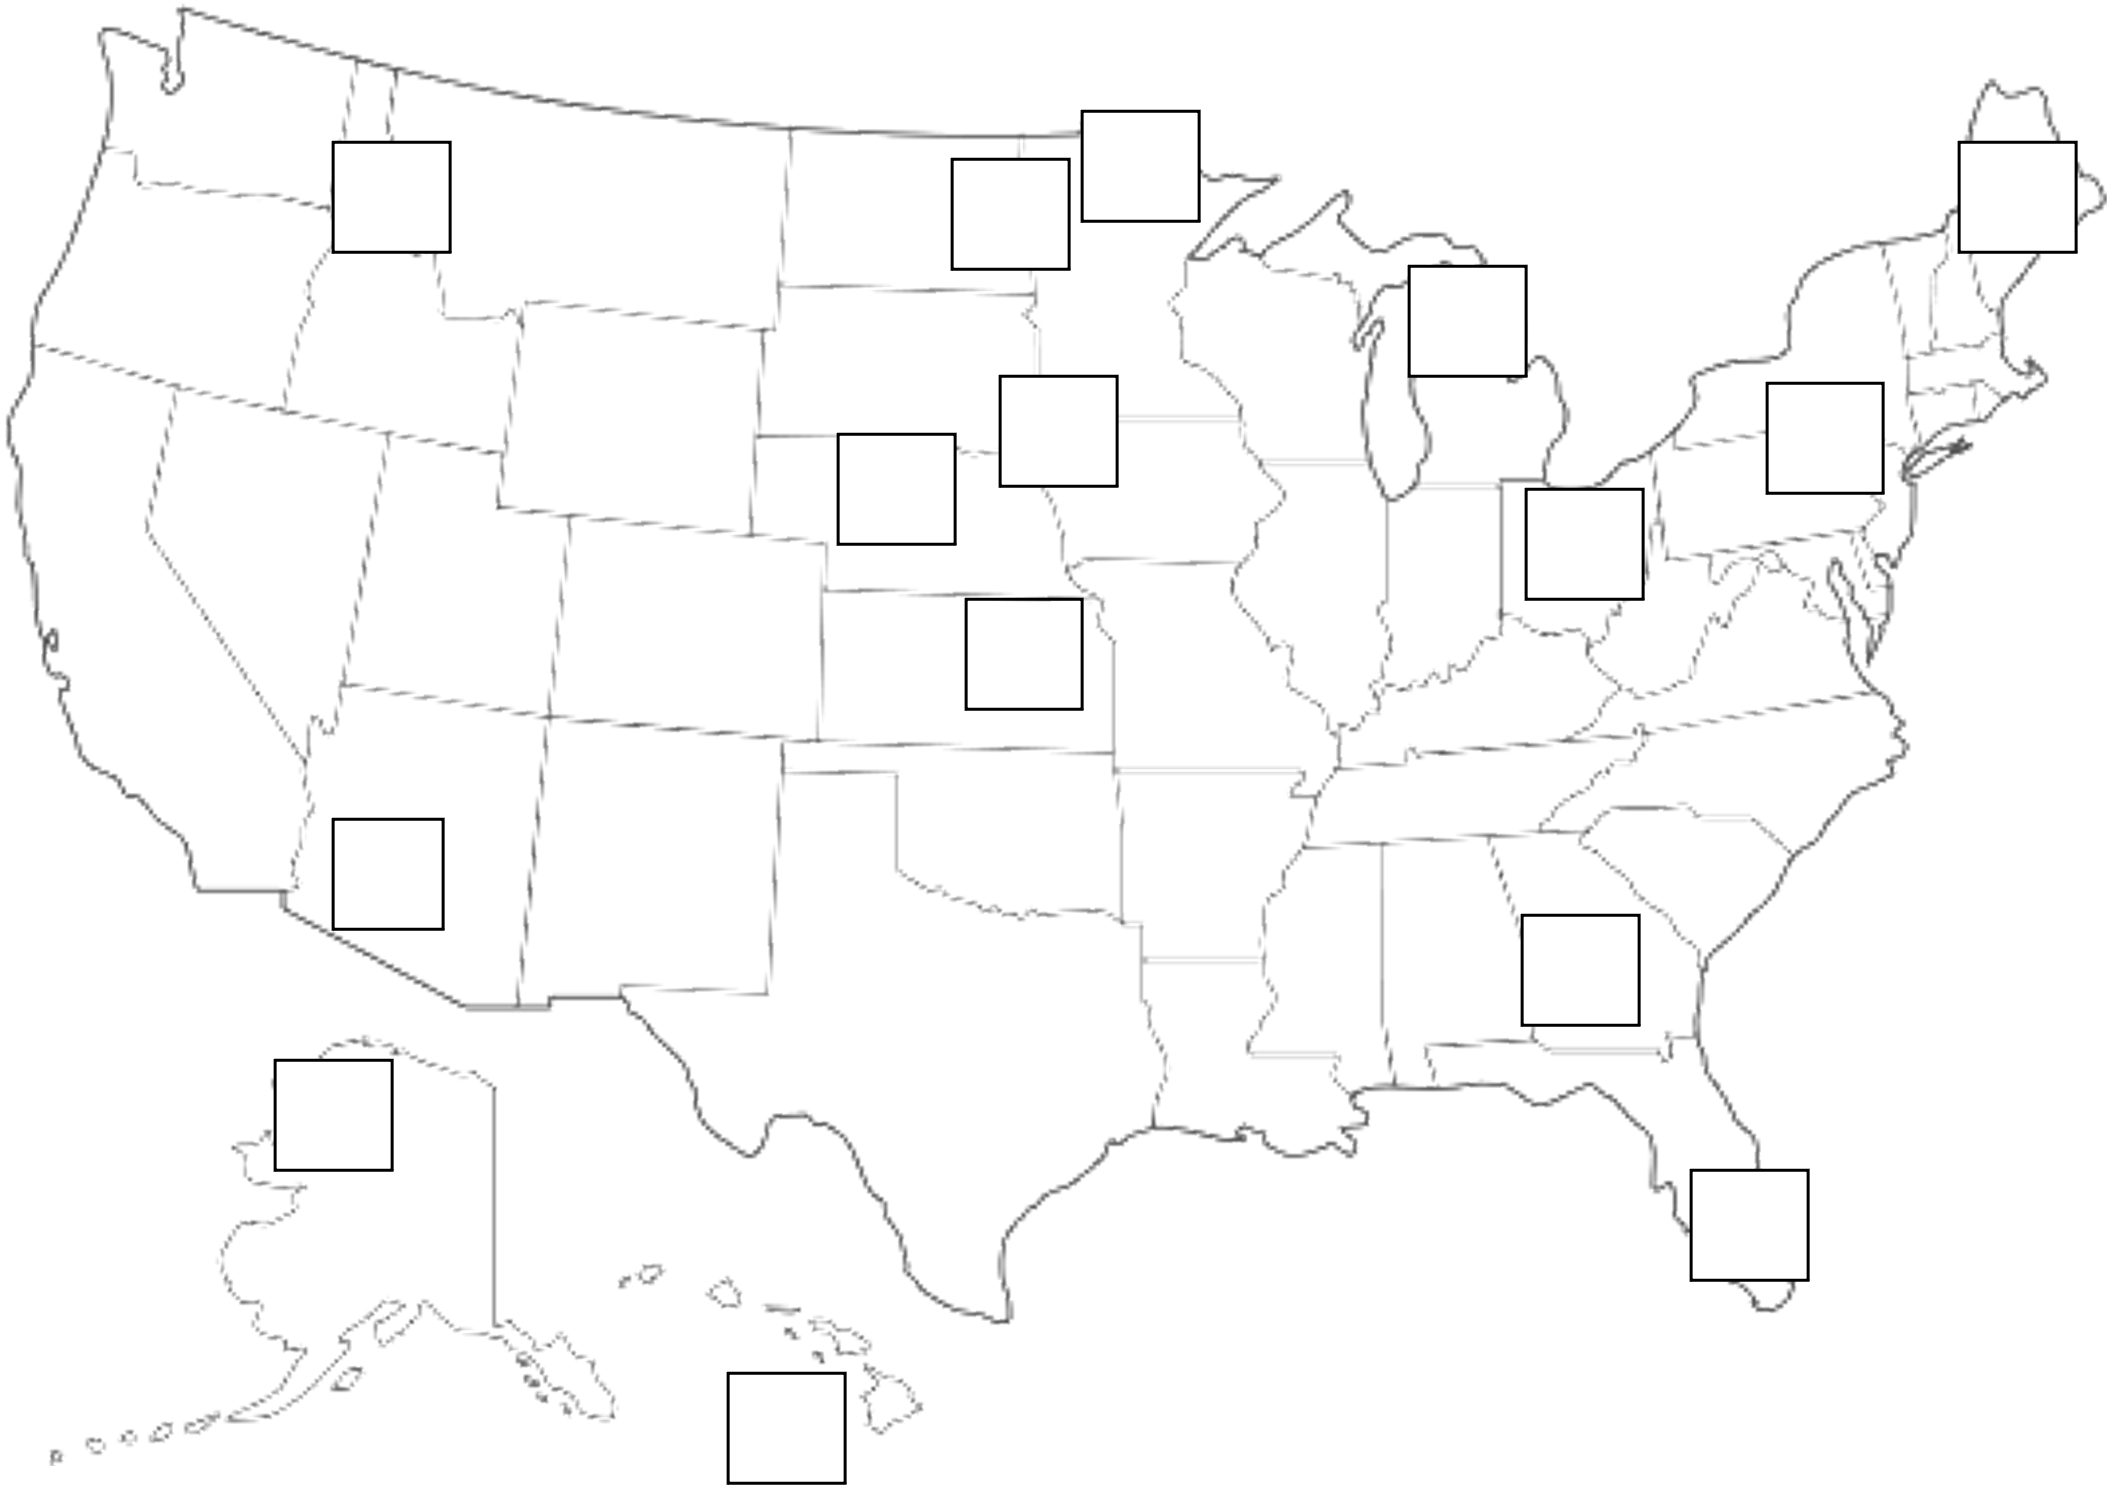
\includegraphics{usa-soil-orders.png}

}

\caption{\label{fig-usa}Soil Orders in the USA}

\end{figure}

 
  \providecommand{\huxb}[2]{\arrayrulecolor[RGB]{#1}\global\arrayrulewidth=#2pt}
  \providecommand{\huxvb}[2]{\color[RGB]{#1}\vrule width #2pt}
  \providecommand{\huxtpad}[1]{\rule{0pt}{#1}}
  \providecommand{\huxbpad}[1]{\rule[-#1]{0pt}{#1}}

\begin{table}[h!]
\begin{centerbox}
\begin{threeparttable}
 
\setlength{\tabcolsep}{0pt}
\begin{tabularx}{0.9\textwidth}{p{0.45\textwidth} p{0.45\textwidth}}


\hhline{}
\arrayrulecolor{black}

\multicolumn{1}{!{\huxvb{0, 0, 0}{0}}m{0.45\textwidth}!{\huxvb{0, 0, 0}{0}}}{\hspace{0pt}\parbox[c]{0.45\textwidth-0pt-4pt}{\huxtpad{0pt + 1em}\centering 1. Alfisols\huxbpad{20pt}}} &
\multicolumn{1}{m{0.45\textwidth}!{\huxvb{0, 0, 0}{0}}}{\hspace{4pt}\parbox[c]{0.45\textwidth-4pt-0pt}{\huxtpad{0pt + 1em}\centering 7. Inceptisols\huxbpad{20pt}}} \tabularnewline[-0.5pt]


\hhline{}
\arrayrulecolor{black}

\multicolumn{1}{!{\huxvb{0, 0, 0}{0}}m{0.45\textwidth}!{\huxvb{0, 0, 0}{0}}}{\hspace{0pt}\parbox[c]{0.45\textwidth-0pt-4pt}{\huxtpad{4pt + 1em}\centering 2. Andisols\huxbpad{20pt}}} &
\multicolumn{1}{m{0.45\textwidth}!{\huxvb{0, 0, 0}{0}}}{\hspace{4pt}\parbox[c]{0.45\textwidth-4pt-0pt}{\huxtpad{4pt + 1em}\centering 8. Mollisols\huxbpad{20pt}}} \tabularnewline[-0.5pt]


\hhline{}
\arrayrulecolor{black}

\multicolumn{1}{!{\huxvb{0, 0, 0}{0}}m{0.45\textwidth}!{\huxvb{0, 0, 0}{0}}}{\hspace{0pt}\parbox[c]{0.45\textwidth-0pt-4pt}{\huxtpad{4pt + 1em}\centering 3. Aridisols\huxbpad{20pt}}} &
\multicolumn{1}{m{0.45\textwidth}!{\huxvb{0, 0, 0}{0}}}{\hspace{4pt}\parbox[c]{0.45\textwidth-4pt-0pt}{\huxtpad{4pt + 1em}\centering 9. Oxisols\huxbpad{20pt}}} \tabularnewline[-0.5pt]


\hhline{}
\arrayrulecolor{black}

\multicolumn{1}{!{\huxvb{0, 0, 0}{0}}m{0.45\textwidth}!{\huxvb{0, 0, 0}{0}}}{\hspace{0pt}\parbox[c]{0.45\textwidth-0pt-4pt}{\huxtpad{4pt + 1em}\centering 4. Entisols\huxbpad{20pt}}} &
\multicolumn{1}{m{0.45\textwidth}!{\huxvb{0, 0, 0}{0}}}{\hspace{4pt}\parbox[c]{0.45\textwidth-4pt-0pt}{\huxtpad{4pt + 1em}\centering 10. Spodosols\huxbpad{20pt}}} \tabularnewline[-0.5pt]


\hhline{}
\arrayrulecolor{black}

\multicolumn{1}{!{\huxvb{0, 0, 0}{0}}m{0.45\textwidth}!{\huxvb{0, 0, 0}{0}}}{\hspace{0pt}\parbox[c]{0.45\textwidth-0pt-4pt}{\huxtpad{4pt + 1em}\centering 5. Gelisols\huxbpad{20pt}}} &
\multicolumn{1}{m{0.45\textwidth}!{\huxvb{0, 0, 0}{0}}}{\hspace{4pt}\parbox[c]{0.45\textwidth-4pt-0pt}{\huxtpad{4pt + 1em}\centering 11. Ultisols\huxbpad{20pt}}} \tabularnewline[-0.5pt]


\hhline{}
\arrayrulecolor{black}

\multicolumn{1}{!{\huxvb{0, 0, 0}{0}}m{0.45\textwidth}!{\huxvb{0, 0, 0}{0}}}{\hspace{0pt}\parbox[c]{0.45\textwidth-0pt-4pt}{\huxtpad{4pt + 1em}\centering 6. Histisols\huxbpad{20pt}}} &
\multicolumn{1}{m{0.45\textwidth}!{\huxvb{0, 0, 0}{0}}}{\hspace{4pt}\parbox[c]{0.45\textwidth-4pt-0pt}{\huxtpad{4pt + 1em}\centering 12. Vertisols\huxbpad{20pt}}} \tabularnewline[-0.5pt]


\hhline{}
\arrayrulecolor{black}
\end{tabularx}
\end{threeparttable}\par\end{centerbox}

\end{table}
 

\hypertarget{investigation-c-nomenclature}{%
\section{INVESTIGATION C:
Nomenclature}\label{investigation-c-nomenclature}}

There are twelve soil orders at the highest hierarchical level of soil
taxonomy. The names for these orders relate to Greek, Latin, or other
root words that reveal something about the soil. Fifty-four suborders
are recognized at the next level of classification. There are over 200
great groups and more than 1,100 subgroups. Soil families have similar
physical and chemical properties that affect their response to
management. The lowest category -- soil series -- is usually named after
a geographic feature in the region in which it was originally found and
described. The taxonomic class includes the prefix plus all the
following syllables, e.g., a Great Group would be ``Haplosaprists'', not
just the prefix ``Haplo-''. To help you recognize syllables, remember
familiar descriptive terms like sapric, hemic, mesic, ustic, udic,
aquic. In addition, look for the prefixes hapl- (simple), orth-
(central), epi- (above), argi- (clay) and psamm- (sandy).

Answer the following questions about soil names. \#1 is already answered
for you.

\begin{enumerate}
\def\labelenumi{\arabic{enumi}.}
\tightlist
\item
  \textbf{(EXAMPLE)} Name the order and suborder for the Okeechobee soil
  (Euic, hyperthermic, Hemic Haplosaprists).
\end{enumerate}

Order - \textbf{Histosol}; Suborder: \textbf{Saprist}

\begin{enumerate}
\def\labelenumi{\alph{enumi}.}
\tightlist
\item
  List two characteristics of the Okeechobee based on the suborder name.
\end{enumerate}

\textbf{Large accumulation of organic materials Sapric organic materials
(well decomposed)}

\begin{enumerate}
\def\labelenumi{\arabic{enumi}.}
\setcounter{enumi}{1}
\tightlist
\item
  Name the family for the Clarion soil (Fine-loamy, mixed, mesic, Typic
  Hapludolls).
\end{enumerate}

~ ~ ~

\begin{enumerate}
\def\labelenumi{\arabic{enumi}.}
\setcounter{enumi}{2}
\tightlist
\item
  Name the order and suborder for the Fargo soil (Fine, smectitic,
  frigid, Typic Epiaquerts).
\end{enumerate}

~ ~ ~

3a. Name one characteristic of the Fargo based on the suborder name.

~ ~ ~

3b. Look at the family name -- what property of this soil might you
predict based on the properties of the dominant mineral?

~ ~ ~

\begin{enumerate}
\def\labelenumi{\arabic{enumi}.}
\setcounter{enumi}{3}
\tightlist
\item
  Name the order and suborder for the Lester soil (Fine-loamy, mixed,
  mesic, Mollic Hapludalfs).
\end{enumerate}

~ ~ ~

4a. Name one characteristic of the Lester based on the suborder name.

~ ~ ~

\begin{enumerate}
\def\labelenumi{\arabic{enumi}.}
\setcounter{enumi}{4}
\tightlist
\item
  Name the order and suborder for the Hubbard soil (Sandy, mixed,
  frigid, Entic Hapludolls).
\end{enumerate}

~ ~ ~

5a. List two characteristics of the Hubbard based on the suborder name.

~ ~ ~

\begin{enumerate}
\def\labelenumi{\arabic{enumi}.}
\setcounter{enumi}{5}
\tightlist
\item
  Name the order and suborder for the Omega soil (Sandy, mixed, frigid,
  Typic Haplorthods).
\end{enumerate}

~ ~ ~

\begin{enumerate}
\def\labelenumi{\arabic{enumi}.}
\setcounter{enumi}{6}
\tightlist
\item
  Name the suborder for the Rifle soil (Euic, frigid, Typic
  Haplohemists).
\end{enumerate}

~ ~ ~

\begin{enumerate}
\def\labelenumi{\arabic{enumi}.}
\setcounter{enumi}{7}
\tightlist
\item
  Name the soil order for the Ves soil (Fine-loamy, mixed, mesic, Calcic
  Hapludolls).
\end{enumerate}

~ ~ ~

\begin{enumerate}
\def\labelenumi{\arabic{enumi}.}
\setcounter{enumi}{8}
\tightlist
\item
  Name the soil order for the Valentine soil (Mixed, mesic, Typic
  Ustipsamments).
\end{enumerate}

~ ~ ~

\bookmarksetup{startatroot}

\hypertarget{legal-land-descriptions-and-soil-survey}{%
\chapter{\texorpdfstring{\textbf{Legal Land Descriptions and Soil
Survey}}{Legal Land Descriptions and Soil Survey}}\label{legal-land-descriptions-and-soil-survey}}

\begin{tcolorbox}[enhanced jigsaw, colframe=quarto-callout-note-color-frame, coltitle=black, arc=.35mm, breakable, bottomrule=.15mm, colback=white, rightrule=.15mm, toprule=.15mm, opacityback=0, bottomtitle=1mm, left=2mm, titlerule=0mm, leftrule=.75mm, opacitybacktitle=0.6, toptitle=1mm, title=\textcolor{quarto-callout-note-color}{\faInfo}\hspace{0.5em}{Objectives}, colbacktitle=quarto-callout-note-color!10!white]

\begin{itemize}
\tightlist
\item
  Understand components of a soil survey.
\item
  Use a legal land description to identify parcels of land.
\end{itemize}

\end{tcolorbox}

\begin{tcolorbox}[enhanced jigsaw, colframe=quarto-callout-tip-color-frame, coltitle=black, arc=.35mm, breakable, bottomrule=.15mm, colback=white, rightrule=.15mm, toprule=.15mm, opacityback=0, bottomtitle=1mm, left=2mm, titlerule=0mm, leftrule=.75mm, opacitybacktitle=0.6, toptitle=1mm, title=\textcolor{quarto-callout-tip-color}{\faLightbulb}\hspace{0.5em}{Key Words \& Concepts}, colbacktitle=quarto-callout-tip-color!10!white]

\begin{itemize}
\tightlist
\item
  Township
\item
  Range
\item
  Principal meridian
\item
  Section
\item
  Soil mapping unit
\item
  Soil name
\item
  Geographic information systems
\end{itemize}

\end{tcolorbox}

\hypertarget{investigation-a-legal-land-descriptions}{%
\section{INVESTIGATION A: Legal Land
Descriptions}\label{investigation-a-legal-land-descriptions}}

A legal description/land description is the method of locating and
describing land in relation to the public land survey system. Land is
broken down into areas called townships. Townships are approximately 6
square miles and are divided into 36 sections (each section being
approximately 640 acres). Townships have two designators:

\begin{enumerate}
\def\labelenumi{\arabic{enumi}.}
\tightlist
\item
  A Township designator (T) that describes the distance and direction
  (north or south) from the Baseline, and
\item
  A Range designator (R) that describes the distance and direction (east
  or west) from the Principal Meridian.
\end{enumerate}

Townships highlighted (with numbers written in the center) in Figure 7
include:

\begin{itemize}
\tightlist
\item
  T4N, R4W
\item
  T3N, R3E
\item
  T1S, R2E
\item
  T3S, R4W
\end{itemize}

The number after the T (township) gives the number of townships N or S
of the Baseline, while the number after the R (range) gives the number
of townships E or W of the Principal Meridian.

\begin{figure}

{\centering 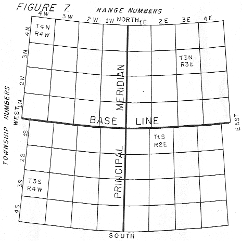
\includegraphics{fig-7-townships.png}

}

\caption{\label{fig-township}Figure 7}

\end{figure}

Sections in each township are numbered consecutively beginning with
number 1 in the northeast corner of the township and counting from right
to left then left to right and so on, weaving back and forth through the
sections of the township in a serpentine manner, and ending with number
36 in the southeast corner.

Additionally, sections may be broken into any number of parcels or
divisions. When you \emph{write} a legal description, always start with
the smallest division first and proceed in steps to the largest
division. When you are attempting \emph{read} a legal description to
find a parcel of land, do the opposite: start with the largest division
first, then proceed to the smallest, reversing the order in which the
legal description is written.

\begin{figure}

{\centering 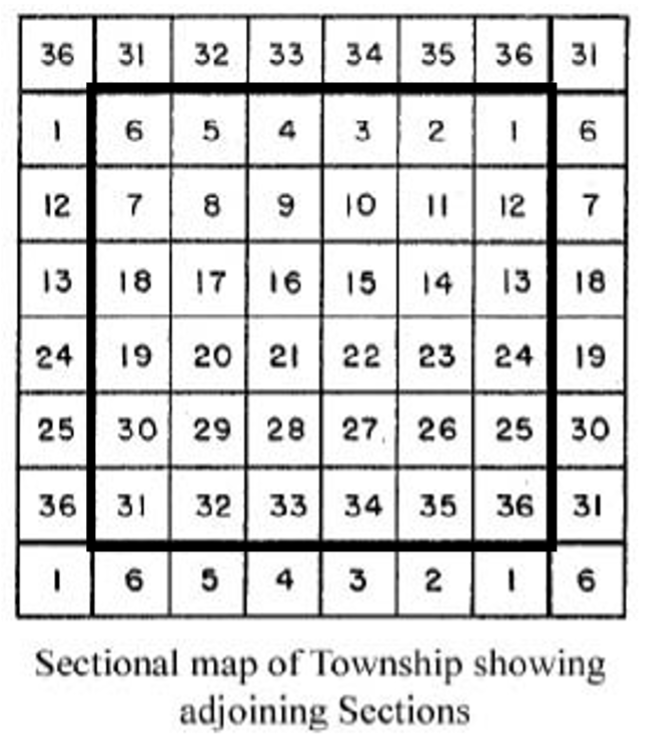
\includegraphics{sections-in-townships.png}

}

\caption{\label{fig-sections}Sections within a Township}

\end{figure}

\begin{figure}

{\centering 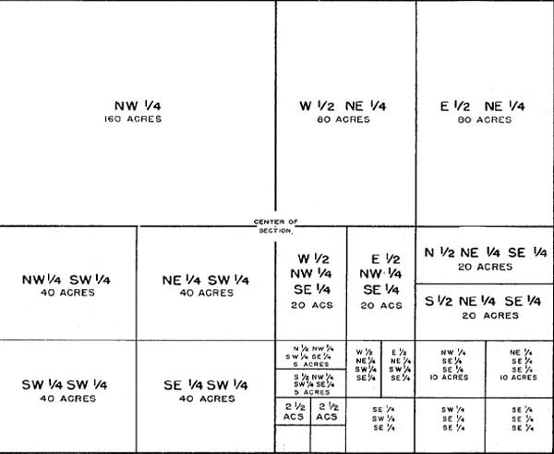
\includegraphics{one-section.png}

}

\caption{\label{fig-labeled}One Section, Labeled}

\end{figure}

\begin{figure}

{\centering 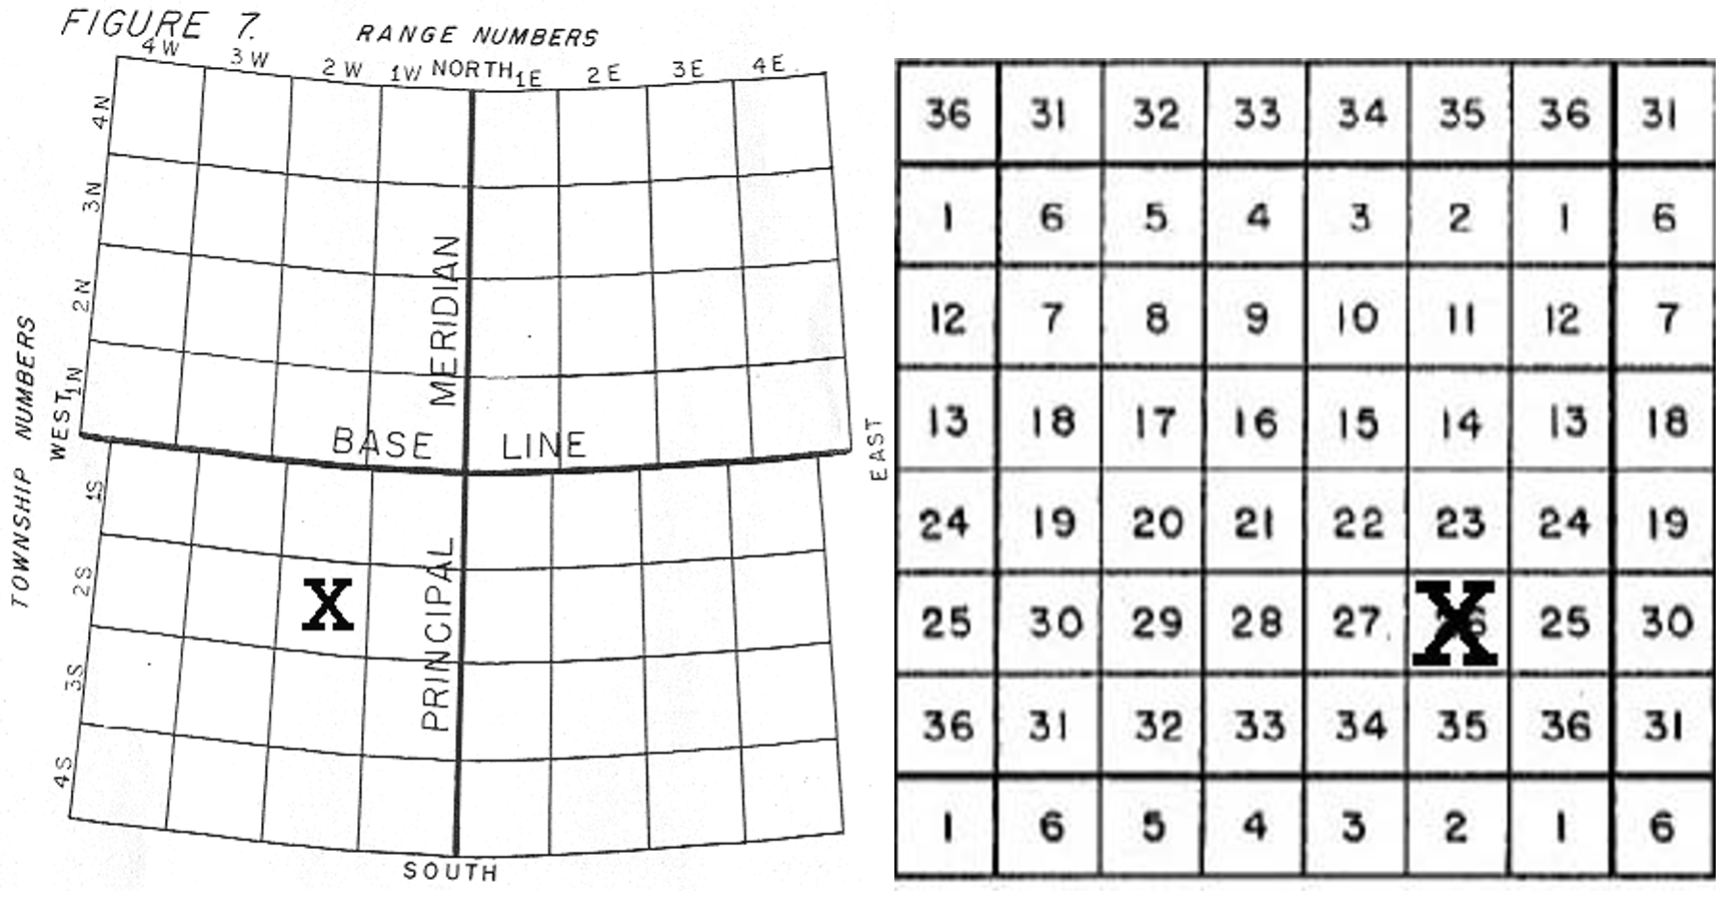
\includegraphics{township-and-section.png}

}

\caption{\label{fig-both}Sections Compared to Their Township}

\end{figure}

\begin{figure}

{\centering 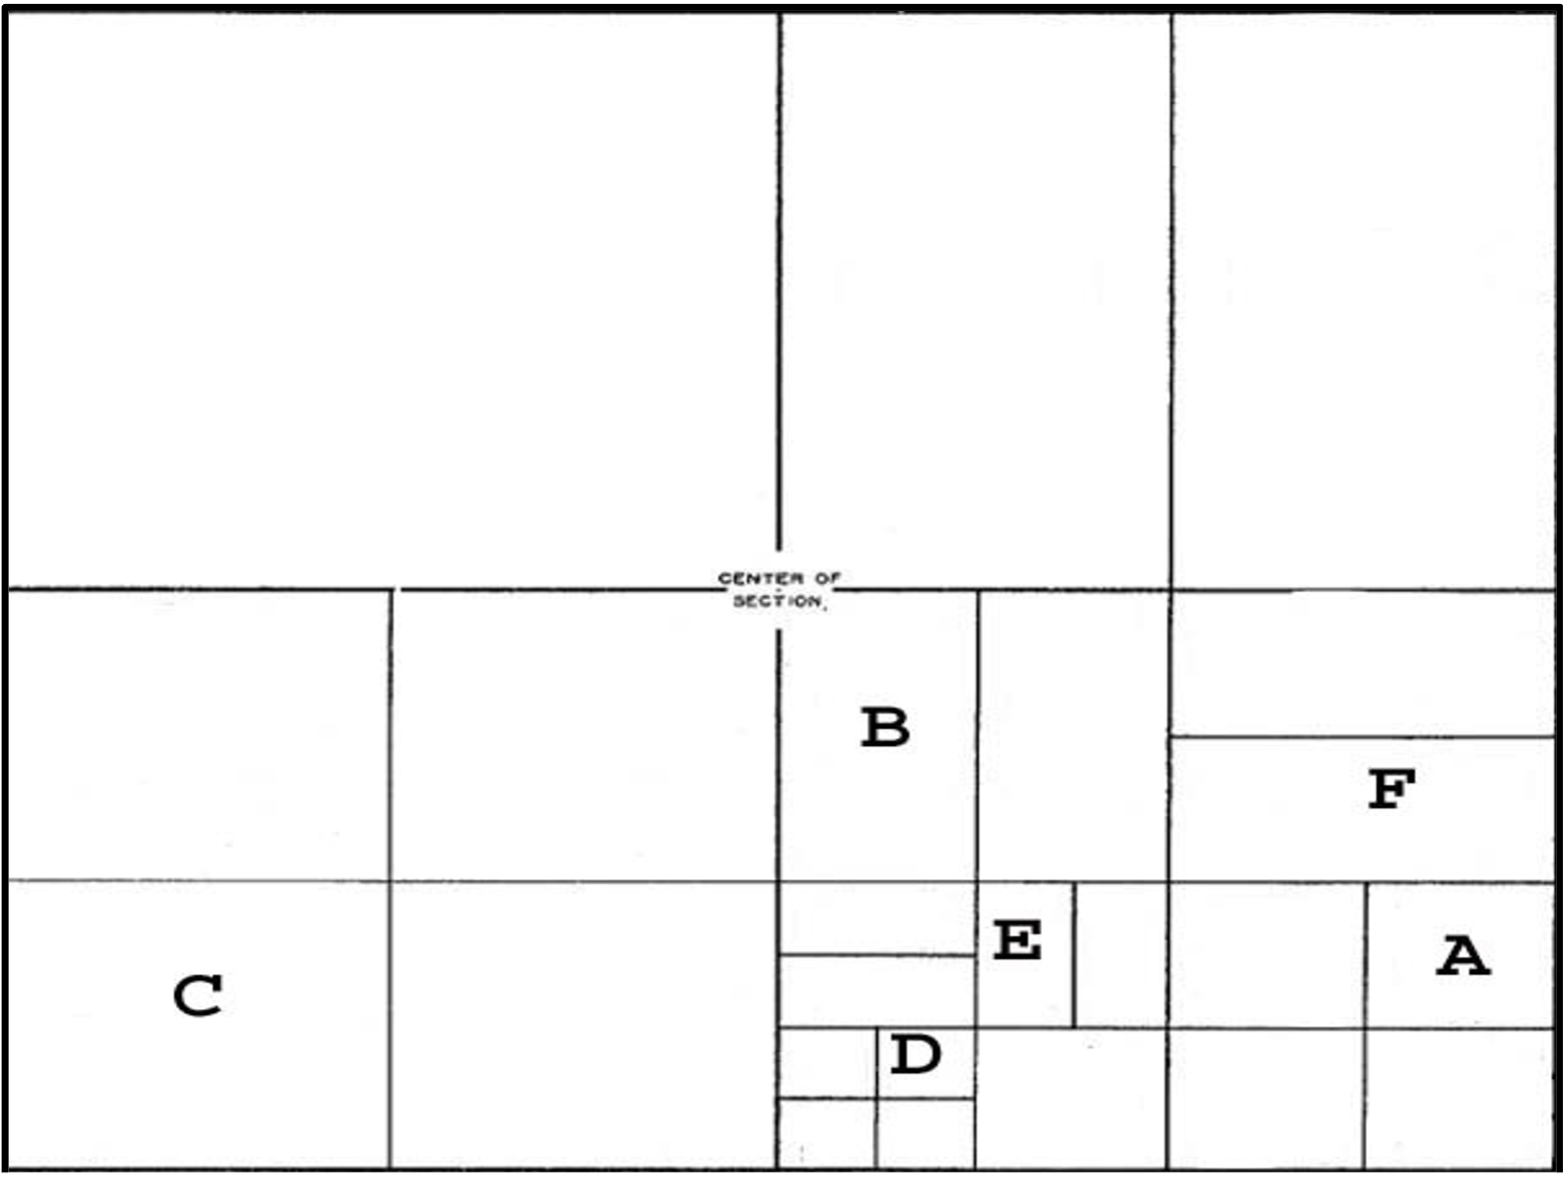
\includegraphics{labeling-sections.png}

}

\caption{\label{fig-practice}Labeling Areas Within a Section}

\end{figure}

Practice writing legal land descriptions by describing areas A through F
below. Make sure you include Township, Range, and Section designators
shown by the X's on the maps above.

 
  \providecommand{\huxb}[2]{\arrayrulecolor[RGB]{#1}\global\arrayrulewidth=#2pt}
  \providecommand{\huxvb}[2]{\color[RGB]{#1}\vrule width #2pt}
  \providecommand{\huxtpad}[1]{\rule{0pt}{#1}}
  \providecommand{\huxbpad}[1]{\rule[-#1]{0pt}{#1}}

\begin{table}[h!]
\begin{centerbox}
\begin{threeparttable}
 
\setlength{\tabcolsep}{0pt}
\begin{tabularx}{0.9\textwidth}{p{0.15\textwidth} p{0.15\textwidth} p{0.15\textwidth} p{0.15\textwidth} p{0.15\textwidth} p{0.15\textwidth}}


\hhline{>{\huxb{0, 0, 0}{1}}->{\huxb{0, 0, 0}{1}}->{\huxb{0, 0, 0}{1}}->{\huxb{0, 0, 0}{1}}->{\huxb{0, 0, 0}{1}}->{\huxb{0, 0, 0}{1}}-}
\arrayrulecolor{black}

\multicolumn{1}{!{\huxvb{0, 0, 0}{1}}m{0.15\textwidth}!{\huxvb{0, 0, 0}{1}}}{\hspace{0pt}\parbox[c]{0.15\textwidth-0pt-4pt}{\huxtpad{0pt + 1em}\centering \textbf{Label}\huxbpad{4pt}}} &
\multicolumn{1}{m{0.15\textwidth}!{\huxvb{0, 0, 0}{1}}}{\hspace{4pt}\parbox[c]{0.15\textwidth-4pt-4pt}{\huxtpad{0pt + 1em}\centering \textbf{Subdivision of Section}\huxbpad{4pt}}} &
\multicolumn{1}{m{0.15\textwidth}!{\huxvb{0, 0, 0}{1}}}{\hspace{4pt}\parbox[c]{0.15\textwidth-4pt-4pt}{\huxtpad{0pt + 1em}\centering \textbf{Section}\huxbpad{4pt}}} &
\multicolumn{1}{m{0.15\textwidth}!{\huxvb{0, 0, 0}{1}}}{\hspace{4pt}\parbox[c]{0.15\textwidth-4pt-4pt}{\huxtpad{0pt + 1em}\centering \textbf{Township}\huxbpad{4pt}}} &
\multicolumn{1}{m{0.15\textwidth}!{\huxvb{0, 0, 0}{1}}}{\hspace{4pt}\parbox[c]{0.15\textwidth-4pt-4pt}{\huxtpad{0pt + 1em}\centering \textbf{Range}\huxbpad{4pt}}} &
\multicolumn{1}{m{0.15\textwidth}!{\huxvb{0, 0, 0}{1}}}{\hspace{4pt}\parbox[c]{0.15\textwidth-4pt-0pt}{\huxtpad{0pt + 1em}\centering \textbf{Acres}\huxbpad{4pt}}} \tabularnewline[-0.5pt]


\hhline{>{\huxb{0, 0, 0}{1}}->{\huxb{0, 0, 0}{1}}->{\huxb{0, 0, 0}{1}}->{\huxb{0, 0, 0}{1}}->{\huxb{0, 0, 0}{1}}->{\huxb{0, 0, 0}{1}}-}
\arrayrulecolor{black}

\multicolumn{1}{!{\huxvb{0, 0, 0}{1}}m{0.15\textwidth}!{\huxvb{0, 0, 0}{1}}}{\hspace{0pt}\parbox[c]{0.15\textwidth-0pt-4pt}{\huxtpad{4pt + 1em}\centering A\huxbpad{4pt}}} &
\multicolumn{1}{m{0.15\textwidth}!{\huxvb{0, 0, 0}{1}}}{\hspace{4pt}\parbox[c]{0.15\textwidth-4pt-4pt}{\huxtpad{4pt + 1em}\centering \huxbpad{4pt}}} &
\multicolumn{1}{m{0.15\textwidth}!{\huxvb{0, 0, 0}{1}}}{\hspace{4pt}\parbox[c]{0.15\textwidth-4pt-4pt}{\huxtpad{4pt + 1em}\centering \huxbpad{4pt}}} &
\multicolumn{1}{m{0.15\textwidth}!{\huxvb{0, 0, 0}{1}}}{\hspace{4pt}\parbox[c]{0.15\textwidth-4pt-4pt}{\huxtpad{4pt + 1em}\centering \huxbpad{4pt}}} &
\multicolumn{1}{m{0.15\textwidth}!{\huxvb{0, 0, 0}{1}}}{\hspace{4pt}\parbox[c]{0.15\textwidth-4pt-4pt}{\huxtpad{4pt + 1em}\centering \huxbpad{4pt}}} &
\multicolumn{1}{m{0.15\textwidth}!{\huxvb{0, 0, 0}{1}}}{\hspace{4pt}\parbox[c]{0.15\textwidth-4pt-0pt}{\huxtpad{4pt + 1em}\centering \huxbpad{4pt}}} \tabularnewline[-0.5pt]


\hhline{>{\huxb{0, 0, 0}{1}}->{\huxb{0, 0, 0}{1}}->{\huxb{0, 0, 0}{1}}->{\huxb{0, 0, 0}{1}}->{\huxb{0, 0, 0}{1}}->{\huxb{0, 0, 0}{1}}-}
\arrayrulecolor{black}

\multicolumn{1}{!{\huxvb{0, 0, 0}{1}}m{0.15\textwidth}!{\huxvb{0, 0, 0}{1}}}{\hspace{0pt}\parbox[c]{0.15\textwidth-0pt-4pt}{\huxtpad{4pt + 1em}\centering B\huxbpad{4pt}}} &
\multicolumn{1}{m{0.15\textwidth}!{\huxvb{0, 0, 0}{1}}}{\hspace{4pt}\parbox[c]{0.15\textwidth-4pt-4pt}{\huxtpad{4pt + 1em}\centering \huxbpad{4pt}}} &
\multicolumn{1}{m{0.15\textwidth}!{\huxvb{0, 0, 0}{1}}}{\hspace{4pt}\parbox[c]{0.15\textwidth-4pt-4pt}{\huxtpad{4pt + 1em}\centering \huxbpad{4pt}}} &
\multicolumn{1}{m{0.15\textwidth}!{\huxvb{0, 0, 0}{1}}}{\hspace{4pt}\parbox[c]{0.15\textwidth-4pt-4pt}{\huxtpad{4pt + 1em}\centering \huxbpad{4pt}}} &
\multicolumn{1}{m{0.15\textwidth}!{\huxvb{0, 0, 0}{1}}}{\hspace{4pt}\parbox[c]{0.15\textwidth-4pt-4pt}{\huxtpad{4pt + 1em}\centering \huxbpad{4pt}}} &
\multicolumn{1}{m{0.15\textwidth}!{\huxvb{0, 0, 0}{1}}}{\hspace{4pt}\parbox[c]{0.15\textwidth-4pt-0pt}{\huxtpad{4pt + 1em}\centering \huxbpad{4pt}}} \tabularnewline[-0.5pt]


\hhline{>{\huxb{0, 0, 0}{1}}->{\huxb{0, 0, 0}{1}}->{\huxb{0, 0, 0}{1}}->{\huxb{0, 0, 0}{1}}->{\huxb{0, 0, 0}{1}}->{\huxb{0, 0, 0}{1}}-}
\arrayrulecolor{black}

\multicolumn{1}{!{\huxvb{0, 0, 0}{1}}m{0.15\textwidth}!{\huxvb{0, 0, 0}{1}}}{\hspace{0pt}\parbox[c]{0.15\textwidth-0pt-4pt}{\huxtpad{4pt + 1em}\centering C\huxbpad{4pt}}} &
\multicolumn{1}{m{0.15\textwidth}!{\huxvb{0, 0, 0}{1}}}{\hspace{4pt}\parbox[c]{0.15\textwidth-4pt-4pt}{\huxtpad{4pt + 1em}\centering \huxbpad{4pt}}} &
\multicolumn{1}{m{0.15\textwidth}!{\huxvb{0, 0, 0}{1}}}{\hspace{4pt}\parbox[c]{0.15\textwidth-4pt-4pt}{\huxtpad{4pt + 1em}\centering \huxbpad{4pt}}} &
\multicolumn{1}{m{0.15\textwidth}!{\huxvb{0, 0, 0}{1}}}{\hspace{4pt}\parbox[c]{0.15\textwidth-4pt-4pt}{\huxtpad{4pt + 1em}\centering \huxbpad{4pt}}} &
\multicolumn{1}{m{0.15\textwidth}!{\huxvb{0, 0, 0}{1}}}{\hspace{4pt}\parbox[c]{0.15\textwidth-4pt-4pt}{\huxtpad{4pt + 1em}\centering \huxbpad{4pt}}} &
\multicolumn{1}{m{0.15\textwidth}!{\huxvb{0, 0, 0}{1}}}{\hspace{4pt}\parbox[c]{0.15\textwidth-4pt-0pt}{\huxtpad{4pt + 1em}\centering \huxbpad{4pt}}} \tabularnewline[-0.5pt]


\hhline{>{\huxb{0, 0, 0}{1}}->{\huxb{0, 0, 0}{1}}->{\huxb{0, 0, 0}{1}}->{\huxb{0, 0, 0}{1}}->{\huxb{0, 0, 0}{1}}->{\huxb{0, 0, 0}{1}}-}
\arrayrulecolor{black}

\multicolumn{1}{!{\huxvb{0, 0, 0}{1}}m{0.15\textwidth}!{\huxvb{0, 0, 0}{1}}}{\hspace{0pt}\parbox[c]{0.15\textwidth-0pt-4pt}{\huxtpad{4pt + 1em}\centering D\huxbpad{4pt}}} &
\multicolumn{1}{m{0.15\textwidth}!{\huxvb{0, 0, 0}{1}}}{\hspace{4pt}\parbox[c]{0.15\textwidth-4pt-4pt}{\huxtpad{4pt + 1em}\centering \huxbpad{4pt}}} &
\multicolumn{1}{m{0.15\textwidth}!{\huxvb{0, 0, 0}{1}}}{\hspace{4pt}\parbox[c]{0.15\textwidth-4pt-4pt}{\huxtpad{4pt + 1em}\centering \huxbpad{4pt}}} &
\multicolumn{1}{m{0.15\textwidth}!{\huxvb{0, 0, 0}{1}}}{\hspace{4pt}\parbox[c]{0.15\textwidth-4pt-4pt}{\huxtpad{4pt + 1em}\centering \huxbpad{4pt}}} &
\multicolumn{1}{m{0.15\textwidth}!{\huxvb{0, 0, 0}{1}}}{\hspace{4pt}\parbox[c]{0.15\textwidth-4pt-4pt}{\huxtpad{4pt + 1em}\centering \huxbpad{4pt}}} &
\multicolumn{1}{m{0.15\textwidth}!{\huxvb{0, 0, 0}{1}}}{\hspace{4pt}\parbox[c]{0.15\textwidth-4pt-0pt}{\huxtpad{4pt + 1em}\centering \huxbpad{4pt}}} \tabularnewline[-0.5pt]


\hhline{>{\huxb{0, 0, 0}{1}}->{\huxb{0, 0, 0}{1}}->{\huxb{0, 0, 0}{1}}->{\huxb{0, 0, 0}{1}}->{\huxb{0, 0, 0}{1}}->{\huxb{0, 0, 0}{1}}-}
\arrayrulecolor{black}

\multicolumn{1}{!{\huxvb{0, 0, 0}{1}}m{0.15\textwidth}!{\huxvb{0, 0, 0}{1}}}{\hspace{0pt}\parbox[c]{0.15\textwidth-0pt-4pt}{\huxtpad{4pt + 1em}\centering E\huxbpad{4pt}}} &
\multicolumn{1}{m{0.15\textwidth}!{\huxvb{0, 0, 0}{1}}}{\hspace{4pt}\parbox[c]{0.15\textwidth-4pt-4pt}{\huxtpad{4pt + 1em}\centering \huxbpad{4pt}}} &
\multicolumn{1}{m{0.15\textwidth}!{\huxvb{0, 0, 0}{1}}}{\hspace{4pt}\parbox[c]{0.15\textwidth-4pt-4pt}{\huxtpad{4pt + 1em}\centering \huxbpad{4pt}}} &
\multicolumn{1}{m{0.15\textwidth}!{\huxvb{0, 0, 0}{1}}}{\hspace{4pt}\parbox[c]{0.15\textwidth-4pt-4pt}{\huxtpad{4pt + 1em}\centering \huxbpad{4pt}}} &
\multicolumn{1}{m{0.15\textwidth}!{\huxvb{0, 0, 0}{1}}}{\hspace{4pt}\parbox[c]{0.15\textwidth-4pt-4pt}{\huxtpad{4pt + 1em}\centering \huxbpad{4pt}}} &
\multicolumn{1}{m{0.15\textwidth}!{\huxvb{0, 0, 0}{1}}}{\hspace{4pt}\parbox[c]{0.15\textwidth-4pt-0pt}{\huxtpad{4pt + 1em}\centering \huxbpad{4pt}}} \tabularnewline[-0.5pt]


\hhline{>{\huxb{0, 0, 0}{1}}->{\huxb{0, 0, 0}{1}}->{\huxb{0, 0, 0}{1}}->{\huxb{0, 0, 0}{1}}->{\huxb{0, 0, 0}{1}}->{\huxb{0, 0, 0}{1}}-}
\arrayrulecolor{black}

\multicolumn{1}{!{\huxvb{0, 0, 0}{1}}m{0.15\textwidth}!{\huxvb{0, 0, 0}{1}}}{\hspace{0pt}\parbox[c]{0.15\textwidth-0pt-4pt}{\huxtpad{4pt + 1em}\centering F\huxbpad{0pt}}} &
\multicolumn{1}{m{0.15\textwidth}!{\huxvb{0, 0, 0}{1}}}{\hspace{4pt}\parbox[c]{0.15\textwidth-4pt-4pt}{\huxtpad{4pt + 1em}\centering \huxbpad{0pt}}} &
\multicolumn{1}{m{0.15\textwidth}!{\huxvb{0, 0, 0}{1}}}{\hspace{4pt}\parbox[c]{0.15\textwidth-4pt-4pt}{\huxtpad{4pt + 1em}\centering \huxbpad{0pt}}} &
\multicolumn{1}{m{0.15\textwidth}!{\huxvb{0, 0, 0}{1}}}{\hspace{4pt}\parbox[c]{0.15\textwidth-4pt-4pt}{\huxtpad{4pt + 1em}\centering \huxbpad{0pt}}} &
\multicolumn{1}{m{0.15\textwidth}!{\huxvb{0, 0, 0}{1}}}{\hspace{4pt}\parbox[c]{0.15\textwidth-4pt-4pt}{\huxtpad{4pt + 1em}\centering \huxbpad{0pt}}} &
\multicolumn{1}{m{0.15\textwidth}!{\huxvb{0, 0, 0}{1}}}{\hspace{4pt}\parbox[c]{0.15\textwidth-4pt-0pt}{\huxtpad{4pt + 1em}\centering \huxbpad{0pt}}} \tabularnewline[-0.5pt]


\hhline{>{\huxb{0, 0, 0}{1}}->{\huxb{0, 0, 0}{1}}->{\huxb{0, 0, 0}{1}}->{\huxb{0, 0, 0}{1}}->{\huxb{0, 0, 0}{1}}->{\huxb{0, 0, 0}{1}}-}
\arrayrulecolor{black}
\end{tabularx}
\end{threeparttable}\par\end{centerbox}

\end{table}
 

\hypertarget{investigation-b-using-web-soil-survey-to-make-land-use-recommendations}{%
\section{INVESTIGATION B: Using Web Soil Survey to Make Land-use
Recommendations}\label{investigation-b-using-web-soil-survey-to-make-land-use-recommendations}}

\textbf{HYPOTHETICAL SITUATION}: The College of Food, Agricultural, and
Natural Resource Sciences has received funding to build a new research,
learning, and outreach center. An alumnus of SOIL 2125 has offered a
quarter section of land in Sibley County, Minnesota as a possible
location of a new center. The legal land description is NE1/4 of Section
10, T113N, R29W, 5th Principal Meridian. The following questions need to
be answered to assess this piece of property.

\begin{enumerate}
\def\labelenumi{\arabic{enumi}.}
\tightlist
\item
  Go to Web Soil Survey:
  http://websoilsurvey.sc.egov.usda.gov/App/HomePage.htm
\item
  Click the green button to start WSS.
\item
  Under ``Quick Navigation'' in the menu bar on the left, click on PLSS
  (Section, Township, Range).
\item
  Enter the information for the property given in the first paragraph,
  above (i.e., Minnesota, 5th Principle Meridian, Section 10, Township
  113N, Range 29W), and click ``View''.
\item
  WSS will take you directly to that section.
\item
  Define the AOI for the parcel. Remember, the property is only the NE ¼
  of the section.
\item
  Once the AOI is defined, click on the ``Soil Map'' tab to view the
  Soil Map.
\item
  Check to ensure you have identified the right parcel by comparing it
  to the figures on the last page of this document.
\item
  Use information from properties and interpretations under the ``Soil
  Data Explorer'' tab to fill in the table below for each map unit.
  Navigate to each item then click ``View Rating''.
\end{enumerate}

\hypertarget{inventory-of-soils-in-ne-14-of-section-10}{%
\subsubsection{Inventory of Soils in NE 1/4 of Section
10}\label{inventory-of-soils-in-ne-14-of-section-10}}

To assess the property, an inventory of soil map units was done. Now the
usefulness of these soils for proposed construction and other uses and
activities is needed. Double check you have the right location with this
figure:

\begin{figure}

{\centering 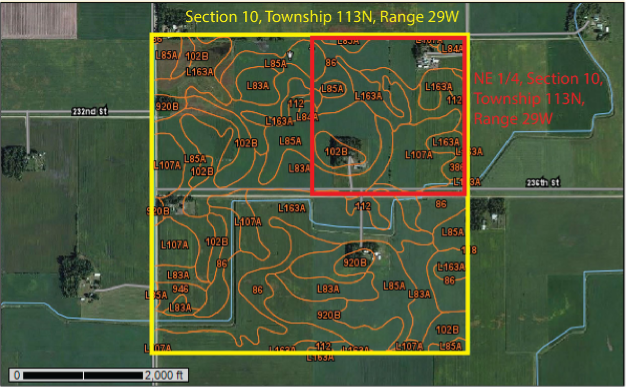
\includegraphics{inventory-of-soil.png}

}

\caption{\label{fig-inventory}Soil Map}

\end{figure}

Use the properties and interpretations from each of the map units given
in Web Soil Survey to fill in the following table. The following
information shows you where to find that piece of information in Web
Soil Survey menus:

\textbf{Suborder}: \textgreater Suitability \& Limitations for Use
\textgreater Land Classification \textgreater Soil Taxonomy
Classification

\textbf{Small Commercial Buildings}: \textgreater Suitability \&
Limitations for Use \textgreater Building Site Development
\textgreater Small Commercial Building

\textbf{Paths and Trails}: \textgreater Suitability \& Limitations for
Use \textgreater Recreational Development \textgreater Paths and Trails

\textbf{At-Grade Septic}: \textgreater Suitability and Limitations for
Use \textgreater Sanitary Facilities \textgreater Septic Tank Absorption
Fields \textgreater At-Grade (MN)

\textbf{Farmland of Statewide Importance}: \textgreater Suitability and
Limitations for Use \textgreater Land Classifications
\textgreater Farmland Classifications

 
  \providecommand{\huxb}[2]{\arrayrulecolor[RGB]{#1}\global\arrayrulewidth=#2pt}
  \providecommand{\huxvb}[2]{\color[RGB]{#1}\vrule width #2pt}
  \providecommand{\huxtpad}[1]{\rule{0pt}{#1}}
  \providecommand{\huxbpad}[1]{\rule[-#1]{0pt}{#1}}

\begin{table}[h!]
\begin{centerbox}
\begin{threeparttable}
 
\setlength{\tabcolsep}{0pt}
\begin{tabularx}{0.9\textwidth}{p{0.128571428571429\textwidth} p{0.128571428571429\textwidth} p{0.128571428571429\textwidth} p{0.128571428571429\textwidth} p{0.128571428571429\textwidth} p{0.128571428571429\textwidth} p{0.128571428571429\textwidth}}


\hhline{>{\huxb{0, 0, 0}{1}}->{\huxb{0, 0, 0}{1}}->{\huxb{0, 0, 0}{1}}->{\huxb{0, 0, 0}{1}}->{\huxb{0, 0, 0}{1}}->{\huxb{0, 0, 0}{1}}->{\huxb{0, 0, 0}{1}}-}
\arrayrulecolor{black}

\multicolumn{1}{!{\huxvb{0, 0, 0}{1}}m{0.128571428571429\textwidth}!{\huxvb{0, 0, 0}{1}}}{\hspace{0pt}\parbox[c]{0.128571428571429\textwidth-0pt-4pt}{\huxtpad{0pt + 1em}\centering \textbf{Symbol}\huxbpad{4pt}}} &
\multicolumn{1}{m{0.128571428571429\textwidth}!{\huxvb{0, 0, 0}{1}}}{\hspace{4pt}\parbox[c]{0.128571428571429\textwidth-4pt-4pt}{\huxtpad{0pt + 1em}\centering \textbf{Soil Order}\huxbpad{4pt}}} &
\multicolumn{1}{m{0.128571428571429\textwidth}!{\huxvb{0, 0, 0}{1}}}{\hspace{4pt}\parbox[c]{0.128571428571429\textwidth-4pt-4pt}{\huxtpad{0pt + 1em}\centering \textbf{Suborder}\huxbpad{4pt}}} &
\multicolumn{1}{m{0.128571428571429\textwidth}!{\huxvb{0, 0, 0}{1}}}{\hspace{4pt}\parbox[c]{0.128571428571429\textwidth-4pt-4pt}{\huxtpad{0pt + 1em}\centering \textbf{Small Commerical Buildings}\huxbpad{4pt}}} &
\multicolumn{1}{m{0.128571428571429\textwidth}!{\huxvb{0, 0, 0}{1}}}{\hspace{4pt}\parbox[c]{0.128571428571429\textwidth-4pt-4pt}{\huxtpad{0pt + 1em}\centering \textbf{Paths and Trails}\huxbpad{4pt}}} &
\multicolumn{1}{m{0.128571428571429\textwidth}!{\huxvb{0, 0, 0}{1}}}{\hspace{4pt}\parbox[c]{0.128571428571429\textwidth-4pt-4pt}{\huxtpad{0pt + 1em}\centering \textbf{At-Grade Septic}\huxbpad{4pt}}} &
\multicolumn{1}{m{0.128571428571429\textwidth}!{\huxvb{0, 0, 0}{1}}}{\hspace{4pt}\parbox[c]{0.128571428571429\textwidth-4pt-0pt}{\huxtpad{0pt + 1em}\centering \textbf{Farmland of Statewide Importance}\huxbpad{4pt}}} \tabularnewline[-0.5pt]


\hhline{>{\huxb{0, 0, 0}{1}}->{\huxb{0, 0, 0}{1}}->{\huxb{0, 0, 0}{1}}->{\huxb{0, 0, 0}{1}}->{\huxb{0, 0, 0}{1}}->{\huxb{0, 0, 0}{1}}->{\huxb{0, 0, 0}{1}}-}
\arrayrulecolor{black}

\multicolumn{1}{!{\huxvb{0, 0, 0}{1}}m{0.128571428571429\textwidth}!{\huxvb{0, 0, 0}{1}}}{\hspace{0pt}\parbox[c]{0.128571428571429\textwidth-0pt-4pt}{\huxtpad{20pt + 1em}\centering 86\huxbpad{20pt}}} &
\multicolumn{1}{m{0.128571428571429\textwidth}!{\huxvb{0, 0, 0}{1}}}{\hspace{4pt}\parbox[c]{0.128571428571429\textwidth-4pt-4pt}{\huxtpad{20pt + 1em}\centering Canisteo clay loam\huxbpad{20pt}}} &
\multicolumn{1}{m{0.128571428571429\textwidth}!{\huxvb{0, 0, 0}{1}}}{\hspace{4pt}\parbox[c]{0.128571428571429\textwidth-4pt-4pt}{\huxtpad{20pt + 1em}\centering \huxbpad{20pt}}} &
\multicolumn{1}{m{0.128571428571429\textwidth}!{\huxvb{0, 0, 0}{1}}}{\hspace{4pt}\parbox[c]{0.128571428571429\textwidth-4pt-4pt}{\huxtpad{20pt + 1em}\centering \huxbpad{20pt}}} &
\multicolumn{1}{m{0.128571428571429\textwidth}!{\huxvb{0, 0, 0}{1}}}{\hspace{4pt}\parbox[c]{0.128571428571429\textwidth-4pt-4pt}{\huxtpad{20pt + 1em}\centering \huxbpad{20pt}}} &
\multicolumn{1}{m{0.128571428571429\textwidth}!{\huxvb{0, 0, 0}{1}}}{\hspace{4pt}\parbox[c]{0.128571428571429\textwidth-4pt-4pt}{\huxtpad{20pt + 1em}\centering \huxbpad{20pt}}} &
\multicolumn{1}{m{0.128571428571429\textwidth}!{\huxvb{0, 0, 0}{1}}}{\hspace{4pt}\parbox[c]{0.128571428571429\textwidth-4pt-0pt}{\huxtpad{20pt + 1em}\centering \huxbpad{20pt}}} \tabularnewline[-0.5pt]


\hhline{>{\huxb{0, 0, 0}{1}}->{\huxb{0, 0, 0}{1}}->{\huxb{0, 0, 0}{1}}->{\huxb{0, 0, 0}{1}}->{\huxb{0, 0, 0}{1}}->{\huxb{0, 0, 0}{1}}->{\huxb{0, 0, 0}{1}}-}
\arrayrulecolor{black}

\multicolumn{1}{!{\huxvb{0, 0, 0}{1}}m{0.128571428571429\textwidth}!{\huxvb{0, 0, 0}{1}}}{\hspace{0pt}\parbox[c]{0.128571428571429\textwidth-0pt-4pt}{\huxtpad{20pt + 1em}\centering 102B\huxbpad{20pt}}} &
\multicolumn{1}{m{0.128571428571429\textwidth}!{\huxvb{0, 0, 0}{1}}}{\hspace{4pt}\parbox[c]{0.128571428571429\textwidth-4pt-4pt}{\huxtpad{20pt + 1em}\centering Clarion loam\huxbpad{20pt}}} &
\multicolumn{1}{m{0.128571428571429\textwidth}!{\huxvb{0, 0, 0}{1}}}{\hspace{4pt}\parbox[c]{0.128571428571429\textwidth-4pt-4pt}{\huxtpad{20pt + 1em}\centering \huxbpad{20pt}}} &
\multicolumn{1}{m{0.128571428571429\textwidth}!{\huxvb{0, 0, 0}{1}}}{\hspace{4pt}\parbox[c]{0.128571428571429\textwidth-4pt-4pt}{\huxtpad{20pt + 1em}\centering \huxbpad{20pt}}} &
\multicolumn{1}{m{0.128571428571429\textwidth}!{\huxvb{0, 0, 0}{1}}}{\hspace{4pt}\parbox[c]{0.128571428571429\textwidth-4pt-4pt}{\huxtpad{20pt + 1em}\centering \huxbpad{20pt}}} &
\multicolumn{1}{m{0.128571428571429\textwidth}!{\huxvb{0, 0, 0}{1}}}{\hspace{4pt}\parbox[c]{0.128571428571429\textwidth-4pt-4pt}{\huxtpad{20pt + 1em}\centering \huxbpad{20pt}}} &
\multicolumn{1}{m{0.128571428571429\textwidth}!{\huxvb{0, 0, 0}{1}}}{\hspace{4pt}\parbox[c]{0.128571428571429\textwidth-4pt-0pt}{\huxtpad{20pt + 1em}\centering \huxbpad{20pt}}} \tabularnewline[-0.5pt]


\hhline{>{\huxb{0, 0, 0}{1}}->{\huxb{0, 0, 0}{1}}->{\huxb{0, 0, 0}{1}}->{\huxb{0, 0, 0}{1}}->{\huxb{0, 0, 0}{1}}->{\huxb{0, 0, 0}{1}}->{\huxb{0, 0, 0}{1}}-}
\arrayrulecolor{black}

\multicolumn{1}{!{\huxvb{0, 0, 0}{1}}m{0.128571428571429\textwidth}!{\huxvb{0, 0, 0}{1}}}{\hspace{0pt}\parbox[c]{0.128571428571429\textwidth-0pt-4pt}{\huxtpad{20pt + 1em}\centering 386\huxbpad{20pt}}} &
\multicolumn{1}{m{0.128571428571429\textwidth}!{\huxvb{0, 0, 0}{1}}}{\hspace{4pt}\parbox[c]{0.128571428571429\textwidth-4pt-4pt}{\huxtpad{20pt + 1em}\centering Okoboji mucky silty clay loam\huxbpad{20pt}}} &
\multicolumn{1}{m{0.128571428571429\textwidth}!{\huxvb{0, 0, 0}{1}}}{\hspace{4pt}\parbox[c]{0.128571428571429\textwidth-4pt-4pt}{\huxtpad{20pt + 1em}\centering \huxbpad{20pt}}} &
\multicolumn{1}{m{0.128571428571429\textwidth}!{\huxvb{0, 0, 0}{1}}}{\hspace{4pt}\parbox[c]{0.128571428571429\textwidth-4pt-4pt}{\huxtpad{20pt + 1em}\centering \huxbpad{20pt}}} &
\multicolumn{1}{m{0.128571428571429\textwidth}!{\huxvb{0, 0, 0}{1}}}{\hspace{4pt}\parbox[c]{0.128571428571429\textwidth-4pt-4pt}{\huxtpad{20pt + 1em}\centering \huxbpad{20pt}}} &
\multicolumn{1}{m{0.128571428571429\textwidth}!{\huxvb{0, 0, 0}{1}}}{\hspace{4pt}\parbox[c]{0.128571428571429\textwidth-4pt-4pt}{\huxtpad{20pt + 1em}\centering \huxbpad{20pt}}} &
\multicolumn{1}{m{0.128571428571429\textwidth}!{\huxvb{0, 0, 0}{1}}}{\hspace{4pt}\parbox[c]{0.128571428571429\textwidth-4pt-0pt}{\huxtpad{20pt + 1em}\centering \huxbpad{20pt}}} \tabularnewline[-0.5pt]


\hhline{>{\huxb{0, 0, 0}{1}}->{\huxb{0, 0, 0}{1}}->{\huxb{0, 0, 0}{1}}->{\huxb{0, 0, 0}{1}}->{\huxb{0, 0, 0}{1}}->{\huxb{0, 0, 0}{1}}->{\huxb{0, 0, 0}{1}}-}
\arrayrulecolor{black}

\multicolumn{1}{!{\huxvb{0, 0, 0}{1}}m{0.128571428571429\textwidth}!{\huxvb{0, 0, 0}{1}}}{\hspace{0pt}\parbox[c]{0.128571428571429\textwidth-0pt-4pt}{\huxtpad{20pt + 1em}\centering L83A\huxbpad{20pt}}} &
\multicolumn{1}{m{0.128571428571429\textwidth}!{\huxvb{0, 0, 0}{1}}}{\hspace{4pt}\parbox[c]{0.128571428571429\textwidth-4pt-4pt}{\huxtpad{20pt + 1em}\centering Webster clay loam\huxbpad{20pt}}} &
\multicolumn{1}{m{0.128571428571429\textwidth}!{\huxvb{0, 0, 0}{1}}}{\hspace{4pt}\parbox[c]{0.128571428571429\textwidth-4pt-4pt}{\huxtpad{20pt + 1em}\centering \huxbpad{20pt}}} &
\multicolumn{1}{m{0.128571428571429\textwidth}!{\huxvb{0, 0, 0}{1}}}{\hspace{4pt}\parbox[c]{0.128571428571429\textwidth-4pt-4pt}{\huxtpad{20pt + 1em}\centering \huxbpad{20pt}}} &
\multicolumn{1}{m{0.128571428571429\textwidth}!{\huxvb{0, 0, 0}{1}}}{\hspace{4pt}\parbox[c]{0.128571428571429\textwidth-4pt-4pt}{\huxtpad{20pt + 1em}\centering \huxbpad{20pt}}} &
\multicolumn{1}{m{0.128571428571429\textwidth}!{\huxvb{0, 0, 0}{1}}}{\hspace{4pt}\parbox[c]{0.128571428571429\textwidth-4pt-4pt}{\huxtpad{20pt + 1em}\centering \huxbpad{20pt}}} &
\multicolumn{1}{m{0.128571428571429\textwidth}!{\huxvb{0, 0, 0}{1}}}{\hspace{4pt}\parbox[c]{0.128571428571429\textwidth-4pt-0pt}{\huxtpad{20pt + 1em}\centering \huxbpad{20pt}}} \tabularnewline[-0.5pt]


\hhline{>{\huxb{0, 0, 0}{1}}->{\huxb{0, 0, 0}{1}}->{\huxb{0, 0, 0}{1}}->{\huxb{0, 0, 0}{1}}->{\huxb{0, 0, 0}{1}}->{\huxb{0, 0, 0}{1}}->{\huxb{0, 0, 0}{1}}-}
\arrayrulecolor{black}

\multicolumn{1}{!{\huxvb{0, 0, 0}{1}}m{0.128571428571429\textwidth}!{\huxvb{0, 0, 0}{1}}}{\hspace{0pt}\parbox[c]{0.128571428571429\textwidth-0pt-4pt}{\huxtpad{20pt + 1em}\centering L84A\huxbpad{20pt}}} &
\multicolumn{1}{m{0.128571428571429\textwidth}!{\huxvb{0, 0, 0}{1}}}{\hspace{4pt}\parbox[c]{0.128571428571429\textwidth-4pt-4pt}{\huxtpad{20pt + 1em}\centering Glencoe clay loam\huxbpad{20pt}}} &
\multicolumn{1}{m{0.128571428571429\textwidth}!{\huxvb{0, 0, 0}{1}}}{\hspace{4pt}\parbox[c]{0.128571428571429\textwidth-4pt-4pt}{\huxtpad{20pt + 1em}\centering \huxbpad{20pt}}} &
\multicolumn{1}{m{0.128571428571429\textwidth}!{\huxvb{0, 0, 0}{1}}}{\hspace{4pt}\parbox[c]{0.128571428571429\textwidth-4pt-4pt}{\huxtpad{20pt + 1em}\centering \huxbpad{20pt}}} &
\multicolumn{1}{m{0.128571428571429\textwidth}!{\huxvb{0, 0, 0}{1}}}{\hspace{4pt}\parbox[c]{0.128571428571429\textwidth-4pt-4pt}{\huxtpad{20pt + 1em}\centering \huxbpad{20pt}}} &
\multicolumn{1}{m{0.128571428571429\textwidth}!{\huxvb{0, 0, 0}{1}}}{\hspace{4pt}\parbox[c]{0.128571428571429\textwidth-4pt-4pt}{\huxtpad{20pt + 1em}\centering \huxbpad{20pt}}} &
\multicolumn{1}{m{0.128571428571429\textwidth}!{\huxvb{0, 0, 0}{1}}}{\hspace{4pt}\parbox[c]{0.128571428571429\textwidth-4pt-0pt}{\huxtpad{20pt + 1em}\centering \huxbpad{20pt}}} \tabularnewline[-0.5pt]


\hhline{>{\huxb{0, 0, 0}{1}}->{\huxb{0, 0, 0}{1}}->{\huxb{0, 0, 0}{1}}->{\huxb{0, 0, 0}{1}}->{\huxb{0, 0, 0}{1}}->{\huxb{0, 0, 0}{1}}->{\huxb{0, 0, 0}{1}}-}
\arrayrulecolor{black}

\multicolumn{1}{!{\huxvb{0, 0, 0}{1}}m{0.128571428571429\textwidth}!{\huxvb{0, 0, 0}{1}}}{\hspace{0pt}\parbox[c]{0.128571428571429\textwidth-0pt-4pt}{\huxtpad{20pt + 1em}\centering L85A\huxbpad{20pt}}} &
\multicolumn{1}{m{0.128571428571429\textwidth}!{\huxvb{0, 0, 0}{1}}}{\hspace{4pt}\parbox[c]{0.128571428571429\textwidth-4pt-4pt}{\huxtpad{20pt + 1em}\centering Nicollet clay loam\huxbpad{20pt}}} &
\multicolumn{1}{m{0.128571428571429\textwidth}!{\huxvb{0, 0, 0}{1}}}{\hspace{4pt}\parbox[c]{0.128571428571429\textwidth-4pt-4pt}{\huxtpad{20pt + 1em}\centering \huxbpad{20pt}}} &
\multicolumn{1}{m{0.128571428571429\textwidth}!{\huxvb{0, 0, 0}{1}}}{\hspace{4pt}\parbox[c]{0.128571428571429\textwidth-4pt-4pt}{\huxtpad{20pt + 1em}\centering \huxbpad{20pt}}} &
\multicolumn{1}{m{0.128571428571429\textwidth}!{\huxvb{0, 0, 0}{1}}}{\hspace{4pt}\parbox[c]{0.128571428571429\textwidth-4pt-4pt}{\huxtpad{20pt + 1em}\centering \huxbpad{20pt}}} &
\multicolumn{1}{m{0.128571428571429\textwidth}!{\huxvb{0, 0, 0}{1}}}{\hspace{4pt}\parbox[c]{0.128571428571429\textwidth-4pt-4pt}{\huxtpad{20pt + 1em}\centering \huxbpad{20pt}}} &
\multicolumn{1}{m{0.128571428571429\textwidth}!{\huxvb{0, 0, 0}{1}}}{\hspace{4pt}\parbox[c]{0.128571428571429\textwidth-4pt-0pt}{\huxtpad{20pt + 1em}\centering \huxbpad{20pt}}} \tabularnewline[-0.5pt]


\hhline{>{\huxb{0, 0, 0}{1}}->{\huxb{0, 0, 0}{1}}->{\huxb{0, 0, 0}{1}}->{\huxb{0, 0, 0}{1}}->{\huxb{0, 0, 0}{1}}->{\huxb{0, 0, 0}{1}}->{\huxb{0, 0, 0}{1}}-}
\arrayrulecolor{black}

\multicolumn{1}{!{\huxvb{0, 0, 0}{1}}m{0.128571428571429\textwidth}!{\huxvb{0, 0, 0}{1}}}{\hspace{0pt}\parbox[c]{0.128571428571429\textwidth-0pt-4pt}{\huxtpad{20pt + 1em}\centering L107A\huxbpad{20pt}}} &
\multicolumn{1}{m{0.128571428571429\textwidth}!{\huxvb{0, 0, 0}{1}}}{\hspace{4pt}\parbox[c]{0.128571428571429\textwidth-4pt-4pt}{\huxtpad{20pt + 1em}\centering Canisteo- Glencoe complex, depressions\huxbpad{20pt}}} &
\multicolumn{1}{m{0.128571428571429\textwidth}!{\huxvb{0, 0, 0}{1}}}{\hspace{4pt}\parbox[c]{0.128571428571429\textwidth-4pt-4pt}{\huxtpad{20pt + 1em}\centering \huxbpad{20pt}}} &
\multicolumn{1}{m{0.128571428571429\textwidth}!{\huxvb{0, 0, 0}{1}}}{\hspace{4pt}\parbox[c]{0.128571428571429\textwidth-4pt-4pt}{\huxtpad{20pt + 1em}\centering \huxbpad{20pt}}} &
\multicolumn{1}{m{0.128571428571429\textwidth}!{\huxvb{0, 0, 0}{1}}}{\hspace{4pt}\parbox[c]{0.128571428571429\textwidth-4pt-4pt}{\huxtpad{20pt + 1em}\centering \huxbpad{20pt}}} &
\multicolumn{1}{m{0.128571428571429\textwidth}!{\huxvb{0, 0, 0}{1}}}{\hspace{4pt}\parbox[c]{0.128571428571429\textwidth-4pt-4pt}{\huxtpad{20pt + 1em}\centering \huxbpad{20pt}}} &
\multicolumn{1}{m{0.128571428571429\textwidth}!{\huxvb{0, 0, 0}{1}}}{\hspace{4pt}\parbox[c]{0.128571428571429\textwidth-4pt-0pt}{\huxtpad{20pt + 1em}\centering \huxbpad{20pt}}} \tabularnewline[-0.5pt]


\hhline{>{\huxb{0, 0, 0}{1}}->{\huxb{0, 0, 0}{1}}->{\huxb{0, 0, 0}{1}}->{\huxb{0, 0, 0}{1}}->{\huxb{0, 0, 0}{1}}->{\huxb{0, 0, 0}{1}}->{\huxb{0, 0, 0}{1}}-}
\arrayrulecolor{black}

\multicolumn{1}{!{\huxvb{0, 0, 0}{1}}m{0.128571428571429\textwidth}!{\huxvb{0, 0, 0}{1}}}{\hspace{0pt}\parbox[c]{0.128571428571429\textwidth-0pt-4pt}{\huxtpad{20pt + 1em}\centering L163A\huxbpad{20pt}}} &
\multicolumn{1}{m{0.128571428571429\textwidth}!{\huxvb{0, 0, 0}{1}}}{\hspace{4pt}\parbox[c]{0.128571428571429\textwidth-4pt-4pt}{\huxtpad{20pt + 1em}\centering Okoboji silty clay loam, depressions\huxbpad{20pt}}} &
\multicolumn{1}{m{0.128571428571429\textwidth}!{\huxvb{0, 0, 0}{1}}}{\hspace{4pt}\parbox[c]{0.128571428571429\textwidth-4pt-4pt}{\huxtpad{20pt + 1em}\centering \huxbpad{20pt}}} &
\multicolumn{1}{m{0.128571428571429\textwidth}!{\huxvb{0, 0, 0}{1}}}{\hspace{4pt}\parbox[c]{0.128571428571429\textwidth-4pt-4pt}{\huxtpad{20pt + 1em}\centering \huxbpad{20pt}}} &
\multicolumn{1}{m{0.128571428571429\textwidth}!{\huxvb{0, 0, 0}{1}}}{\hspace{4pt}\parbox[c]{0.128571428571429\textwidth-4pt-4pt}{\huxtpad{20pt + 1em}\centering \huxbpad{20pt}}} &
\multicolumn{1}{m{0.128571428571429\textwidth}!{\huxvb{0, 0, 0}{1}}}{\hspace{4pt}\parbox[c]{0.128571428571429\textwidth-4pt-4pt}{\huxtpad{20pt + 1em}\centering \huxbpad{20pt}}} &
\multicolumn{1}{m{0.128571428571429\textwidth}!{\huxvb{0, 0, 0}{1}}}{\hspace{4pt}\parbox[c]{0.128571428571429\textwidth-4pt-0pt}{\huxtpad{20pt + 1em}\centering \huxbpad{20pt}}} \tabularnewline[-0.5pt]


\hhline{>{\huxb{0, 0, 0}{1}}->{\huxb{0, 0, 0}{1}}->{\huxb{0, 0, 0}{1}}->{\huxb{0, 0, 0}{1}}->{\huxb{0, 0, 0}{1}}->{\huxb{0, 0, 0}{1}}->{\huxb{0, 0, 0}{1}}-}
\arrayrulecolor{black}
\end{tabularx}
\end{threeparttable}\par\end{centerbox}

\end{table}
 

The College would like to construct the facilities listed in the table
below. Indicate in the table on what soil map unit(s) in this piece of
land you would locate each. Include the symbol and soil series for each
unit as listed in the previous table. Ignore existing building locations
in your choices as the College wishes to make the best possible land-use
choices in each case, regardless of current development.

Make suitability determinations based on the Soil Survey data alone.

 
  \providecommand{\huxb}[2]{\arrayrulecolor[RGB]{#1}\global\arrayrulewidth=#2pt}
  \providecommand{\huxvb}[2]{\color[RGB]{#1}\vrule width #2pt}
  \providecommand{\huxtpad}[1]{\rule{0pt}{#1}}
  \providecommand{\huxbpad}[1]{\rule[-#1]{0pt}{#1}}

\begin{table}[h!]
\begin{centerbox}
\begin{threeparttable}
 
\setlength{\tabcolsep}{0pt}
\begin{tabularx}{0.9\textwidth}{p{0.45\textwidth} p{0.45\textwidth}}


\hhline{>{\huxb{0, 0, 0}{1}}->{\huxb{0, 0, 0}{1}}-}
\arrayrulecolor{black}

\multicolumn{1}{!{\huxvb{0, 0, 0}{1}}m{0.45\textwidth}!{\huxvb{0, 0, 0}{1}}}{\hspace{0pt}\parbox[c]{0.45\textwidth-0pt-4pt}{\huxtpad{0pt + 1em}\centering \textbf{Facility}\huxbpad{4pt}}} &
\multicolumn{1}{m{0.45\textwidth}!{\huxvb{0, 0, 0}{1}}}{\hspace{4pt}\parbox[c]{0.45\textwidth-4pt-0pt}{\huxtpad{0pt + 1em}\centering \textbf{Most suitable soil map unit(s) and soil series names}\huxbpad{4pt}}} \tabularnewline[-0.5pt]


\hhline{>{\huxb{0, 0, 0}{1}}->{\huxb{0, 0, 0}{1}}-}
\arrayrulecolor{black}

\multicolumn{1}{!{\huxvb{0, 0, 0}{1}}m{0.45\textwidth}!{\huxvb{0, 0, 0}{1}}}{\hspace{0pt}\parbox[c]{0.45\textwidth-0pt-4pt}{\huxtpad{20pt + 1em}\centering Plant, Animal, and Environmental Science Building (small commercial)\huxbpad{20pt}}} &
\multicolumn{1}{m{0.45\textwidth}!{\huxvb{0, 0, 0}{1}}}{\hspace{4pt}\parbox[c]{0.45\textwidth-4pt-0pt}{\huxtpad{20pt + 1em}\centering \huxbpad{20pt}}} \tabularnewline[-0.5pt]


\hhline{>{\huxb{0, 0, 0}{1}}->{\huxb{0, 0, 0}{1}}-}
\arrayrulecolor{black}

\multicolumn{1}{!{\huxvb{0, 0, 0}{1}}m{0.45\textwidth}!{\huxvb{0, 0, 0}{1}}}{\hspace{0pt}\parbox[c]{0.45\textwidth-0pt-4pt}{\huxtpad{20pt + 1em}\centering Septic system for whole unit (At-Grade Septic)\huxbpad{20pt}}} &
\multicolumn{1}{m{0.45\textwidth}!{\huxvb{0, 0, 0}{1}}}{\hspace{4pt}\parbox[c]{0.45\textwidth-4pt-0pt}{\huxtpad{20pt + 1em}\centering \huxbpad{20pt}}} \tabularnewline[-0.5pt]


\hhline{>{\huxb{0, 0, 0}{1}}->{\huxb{0, 0, 0}{1}}-}
\arrayrulecolor{black}

\multicolumn{1}{!{\huxvb{0, 0, 0}{1}}m{0.45\textwidth}!{\huxvb{0, 0, 0}{1}}}{\hspace{0pt}\parbox[c]{0.45\textwidth-0pt-4pt}{\huxtpad{20pt + 1em}\centering Restored wetland (Aquic Suborders and/or Histosols\huxbpad{20pt}}} &
\multicolumn{1}{m{0.45\textwidth}!{\huxvb{0, 0, 0}{1}}}{\hspace{4pt}\parbox[c]{0.45\textwidth-4pt-0pt}{\huxtpad{20pt + 1em}\centering \huxbpad{20pt}}} \tabularnewline[-0.5pt]


\hhline{>{\huxb{0, 0, 0}{1}}->{\huxb{0, 0, 0}{1}}-}
\arrayrulecolor{black}

\multicolumn{1}{!{\huxvb{0, 0, 0}{1}}m{0.45\textwidth}!{\huxvb{0, 0, 0}{1}}}{\hspace{0pt}\parbox[c]{0.45\textwidth-0pt-4pt}{\huxtpad{20pt + 1em}\centering Permanent soil pit displayed Farmland of Statewide Importance\huxbpad{20pt}}} &
\multicolumn{1}{m{0.45\textwidth}!{\huxvb{0, 0, 0}{1}}}{\hspace{4pt}\parbox[c]{0.45\textwidth-4pt-0pt}{\huxtpad{20pt + 1em}\centering \huxbpad{20pt}}} \tabularnewline[-0.5pt]


\hhline{>{\huxb{0, 0, 0}{1}}->{\huxb{0, 0, 0}{1}}-}
\arrayrulecolor{black}

\multicolumn{1}{!{\huxvb{0, 0, 0}{1}}m{0.45\textwidth}!{\huxvb{0, 0, 0}{1}}}{\hspace{0pt}\parbox[c]{0.45\textwidth-0pt-4pt}{\huxtpad{20pt + 1em}\centering Nature and bike trail (Paths and Trails)\huxbpad{20pt}}} &
\multicolumn{1}{m{0.45\textwidth}!{\huxvb{0, 0, 0}{1}}}{\hspace{4pt}\parbox[c]{0.45\textwidth-4pt-0pt}{\huxtpad{20pt + 1em}\centering \huxbpad{20pt}}} \tabularnewline[-0.5pt]


\hhline{>{\huxb{0, 0, 0}{1}}->{\huxb{0, 0, 0}{1}}-}
\arrayrulecolor{black}
\end{tabularx}
\end{threeparttable}\par\end{centerbox}

\end{table}
 

\bookmarksetup{startatroot}

\hypertarget{soil-management-chemical}{%
\chapter{\texorpdfstring{\textbf{Soil Management:
Chemical}}{Soil Management: Chemical}}\label{soil-management-chemical}}

\begin{tcolorbox}[enhanced jigsaw, colframe=quarto-callout-note-color-frame, coltitle=black, arc=.35mm, breakable, bottomrule=.15mm, colback=white, rightrule=.15mm, toprule=.15mm, opacityback=0, bottomtitle=1mm, left=2mm, titlerule=0mm, leftrule=.75mm, opacitybacktitle=0.6, toptitle=1mm, title=\textcolor{quarto-callout-note-color}{\faInfo}\hspace{0.5em}{Objectives}, colbacktitle=quarto-callout-note-color!10!white]

\begin{itemize}
\tightlist
\item
  Understand factors that affect nutrient management
\item
  Learn how to read a soil test report
\item
  Determine the best nutrient source to meet soil test nutrient
  recommendations
\item
  Observe the impact of lime and acid on high and low base saturation
  soils
\item
  Interact with personal soil samples to determine general idea of
  nitrate and pH levels
\end{itemize}

\end{tcolorbox}

\begin{tcolorbox}[enhanced jigsaw, colframe=quarto-callout-tip-color-frame, coltitle=black, arc=.35mm, breakable, bottomrule=.15mm, colback=white, rightrule=.15mm, toprule=.15mm, opacityback=0, bottomtitle=1mm, left=2mm, titlerule=0mm, leftrule=.75mm, opacitybacktitle=0.6, toptitle=1mm, title=\textcolor{quarto-callout-tip-color}{\faLightbulb}\hspace{0.5em}{Key Words \& Concepts}, colbacktitle=quarto-callout-tip-color!10!white]

\begin{itemize}
\tightlist
\item
  Nutrient management
\item
  Soil testing
\item
  Fertilizer grade
\end{itemize}

\end{tcolorbox}

\hypertarget{pre-lab-prep}{%
\section{PRE-LAB PREP}\label{pre-lab-prep}}

Collect approximately 1 cup of soil from a garden or farm. Make sure to
sample only to a 0-3 inch depth. \textbf{Optional}: Determine the
texture of your soil sample using the ribbon method and record it in
this week's texture contest.

~

\hypertarget{investigation-a-macronutrient-cycles}{%
\section{INVESTIGATION A: Macronutrient
Cycles}\label{investigation-a-macronutrient-cycles}}

For this investigation, we will consider N-P-K, three essential plant
macronutrients. You may recognize these letters from bags of fertilizer
in the hardware store or garden centers. We have gone over the Nitrogen
cycle in detail as Nitrogen is ubiquitously the most limiting nutrient
for plant growth. Phosphorus and Potassium undergo their own cycles
which are unique processes. The following exercise will provide an
opportunity to understand the characteristics and movement of these
three major macronutrients.

Fill in the following information pertaining to the nutrient cycles.

 
  \providecommand{\huxb}[2]{\arrayrulecolor[RGB]{#1}\global\arrayrulewidth=#2pt}
  \providecommand{\huxvb}[2]{\color[RGB]{#1}\vrule width #2pt}
  \providecommand{\huxtpad}[1]{\rule{0pt}{#1}}
  \providecommand{\huxbpad}[1]{\rule[-#1]{0pt}{#1}}

\begin{table}[h!]
\begin{centerbox}
\begin{threeparttable}
 
\setlength{\tabcolsep}{0pt}
\begin{tabularx}{0.9\textwidth}{p{0.225\textwidth} p{0.225\textwidth} p{0.225\textwidth} p{0.225\textwidth}}


\hhline{>{\huxb{0, 0, 0}{1}}->{\huxb{0, 0, 0}{1}}->{\huxb{0, 0, 0}{1}}->{\huxb{0, 0, 0}{1}}-}
\arrayrulecolor{black}

\multicolumn{1}{!{\huxvb{0, 0, 0}{1}}m{0.225\textwidth}!{\huxvb{0, 0, 0}{1}}}{\hspace{0pt}\parbox[c]{0.225\textwidth-0pt-4pt}{\huxtpad{0pt + 1em}\centering \textbf{Nutrient Cycle}\huxbpad{4pt}}} &
\multicolumn{1}{m{0.225\textwidth}!{\huxvb{0, 0, 0}{1}}}{\hspace{4pt}\parbox[c]{0.225\textwidth-4pt-4pt}{\huxtpad{0pt + 1em}\centering \textbf{Is Mineral Weathering a Factor? (Yes/No)}\huxbpad{4pt}}} &
\multicolumn{1}{m{0.225\textwidth}!{\huxvb{0, 0, 0}{1}}}{\hspace{4pt}\parbox[c]{0.225\textwidth-4pt-4pt}{\huxtpad{0pt + 1em}\centering \textbf{Is Soil Organic Matter a Factor? (Yes/No)}\huxbpad{4pt}}} &
\multicolumn{1}{m{0.225\textwidth}!{\huxvb{0, 0, 0}{1}}}{\hspace{4pt}\parbox[c]{0.225\textwidth-4pt-0pt}{\huxtpad{0pt + 1em}\centering \textbf{What is the Plant Available Form?}\huxbpad{4pt}}} \tabularnewline[-0.5pt]


\hhline{>{\huxb{0, 0, 0}{1}}->{\huxb{0, 0, 0}{1}}->{\huxb{0, 0, 0}{1}}->{\huxb{0, 0, 0}{1}}-}
\arrayrulecolor{black}

\multicolumn{1}{!{\huxvb{0, 0, 0}{1}}m{0.225\textwidth}!{\huxvb{0, 0, 0}{1}}}{\hspace{0pt}\parbox[c]{0.225\textwidth-0pt-4pt}{\huxtpad{20pt + 1em}\centering N\huxbpad{20pt}}} &
\multicolumn{1}{m{0.225\textwidth}!{\huxvb{0, 0, 0}{1}}}{\hspace{4pt}\parbox[c]{0.225\textwidth-4pt-4pt}{\huxtpad{20pt + 1em}\centering \huxbpad{20pt}}} &
\multicolumn{1}{m{0.225\textwidth}!{\huxvb{0, 0, 0}{1}}}{\hspace{4pt}\parbox[c]{0.225\textwidth-4pt-4pt}{\huxtpad{20pt + 1em}\centering \huxbpad{20pt}}} &
\multicolumn{1}{m{0.225\textwidth}!{\huxvb{0, 0, 0}{1}}}{\hspace{4pt}\parbox[c]{0.225\textwidth-4pt-0pt}{\huxtpad{20pt + 1em}\centering \huxbpad{20pt}}} \tabularnewline[-0.5pt]


\hhline{>{\huxb{0, 0, 0}{1}}->{\huxb{0, 0, 0}{1}}->{\huxb{0, 0, 0}{1}}->{\huxb{0, 0, 0}{1}}-}
\arrayrulecolor{black}

\multicolumn{1}{!{\huxvb{0, 0, 0}{1}}m{0.225\textwidth}!{\huxvb{0, 0, 0}{1}}}{\hspace{0pt}\parbox[c]{0.225\textwidth-0pt-4pt}{\huxtpad{20pt + 1em}\centering P\huxbpad{20pt}}} &
\multicolumn{1}{m{0.225\textwidth}!{\huxvb{0, 0, 0}{1}}}{\hspace{4pt}\parbox[c]{0.225\textwidth-4pt-4pt}{\huxtpad{20pt + 1em}\centering \huxbpad{20pt}}} &
\multicolumn{1}{m{0.225\textwidth}!{\huxvb{0, 0, 0}{1}}}{\hspace{4pt}\parbox[c]{0.225\textwidth-4pt-4pt}{\huxtpad{20pt + 1em}\centering \huxbpad{20pt}}} &
\multicolumn{1}{m{0.225\textwidth}!{\huxvb{0, 0, 0}{1}}}{\hspace{4pt}\parbox[c]{0.225\textwidth-4pt-0pt}{\huxtpad{20pt + 1em}\centering \huxbpad{20pt}}} \tabularnewline[-0.5pt]


\hhline{>{\huxb{0, 0, 0}{1}}->{\huxb{0, 0, 0}{1}}->{\huxb{0, 0, 0}{1}}->{\huxb{0, 0, 0}{1}}-}
\arrayrulecolor{black}

\multicolumn{1}{!{\huxvb{0, 0, 0}{1}}m{0.225\textwidth}!{\huxvb{0, 0, 0}{1}}}{\hspace{0pt}\parbox[c]{0.225\textwidth-0pt-4pt}{\huxtpad{20pt + 1em}\centering K\huxbpad{20pt}}} &
\multicolumn{1}{m{0.225\textwidth}!{\huxvb{0, 0, 0}{1}}}{\hspace{4pt}\parbox[c]{0.225\textwidth-4pt-4pt}{\huxtpad{20pt + 1em}\centering \huxbpad{20pt}}} &
\multicolumn{1}{m{0.225\textwidth}!{\huxvb{0, 0, 0}{1}}}{\hspace{4pt}\parbox[c]{0.225\textwidth-4pt-4pt}{\huxtpad{20pt + 1em}\centering \huxbpad{20pt}}} &
\multicolumn{1}{m{0.225\textwidth}!{\huxvb{0, 0, 0}{1}}}{\hspace{4pt}\parbox[c]{0.225\textwidth-4pt-0pt}{\huxtpad{20pt + 1em}\centering \huxbpad{20pt}}} \tabularnewline[-0.5pt]


\hhline{>{\huxb{0, 0, 0}{1}}->{\huxb{0, 0, 0}{1}}->{\huxb{0, 0, 0}{1}}->{\huxb{0, 0, 0}{1}}-}
\arrayrulecolor{black}
\end{tabularx}
\end{threeparttable}\par\end{centerbox}

\end{table}
 

\begin{enumerate}
\def\labelenumi{\arabic{enumi}.}
\tightlist
\item
  The plant available form of phosphorus PO43- is an anion, yet
  phosphorus is not generally susceptible to leaching, unlike nitrogen.
  Why?
\end{enumerate}

~ ~ ~

\begin{enumerate}
\def\labelenumi{\arabic{enumi}.}
\setcounter{enumi}{1}
\tightlist
\item
  How is potassium (K) availability controlled by mineral weathering?
\end{enumerate}

~ ~ ~

\begin{enumerate}
\def\labelenumi{\arabic{enumi}.}
\setcounter{enumi}{2}
\tightlist
\item
  In Minnesota, what is the best time to soil test for an accurate
  understanding of plant available nitrogen (N)?
\end{enumerate}

~ ~ ~

\hypertarget{investigation-b-measuring-soil-ph-and-nitrate-levels-with-test-strips}{%
\section{INVESTIGATION B: Measuring Soil pH and Nitrate Levels with Test
Strips}\label{investigation-b-measuring-soil-ph-and-nitrate-levels-with-test-strips}}

Below are instructions for prepping two different set ups for soil
analysis using pH and nitrate strips. \textbf{Preparing them in advance
will be helpful to you as they need 10 mins before reading.} We are
using test strips in the lab to provide a rapid indication of the pH and
nitrate in your soil sample. However, note that for making detailed
decisions regarding soil management and plant growth, you would want a
more accurate, laboratory measurement of pH and nitrate.

\textbf{Soil pH}

\begin{enumerate}
\def\labelenumi{\arabic{enumi}.}
\item
  Locate your soil (check-in with TA on duty to provide your sample to
  you), 50 ml tube, DI water, pH strips.
\item
  Fill the 50 ml tube with 10 ml of your soil.
\item
  Saturate the soil with DI water and fill up to the 20 mL line. This
  makes a 1:1 ratio of soil/water.
\item
  Shake vigorously for roughly 30 sec and let sit for 10 mins.
\item
  When ready to read, take a pH strip and dip into the tube. Try not to
  dip directly in the soil.
\item
  The pH paper will react; line it up with the color chart to what
  closely matches the strip. Record your result.
\end{enumerate}

\textbf{Nitrate}

\begin{enumerate}
\def\labelenumi{\arabic{enumi}.}
\item
  Locate your soil (soil from same sample as for your pH reading),
  filter paper, funnel, catch receptacle, DI water, nitrate strip.
\item
  Fold the filter paper into a cone shape. You can do this by folding it
  in half and then in half once more (making it into a quarter). Open
  the filter up to make a cone shape and place it in a funnel.
\item
  Pre wet the paper by squirting DI water around it. It doesn't need to
  be saturated but wetting it will help the filtering go faster.
\item
  Put a scoop of your soil (approximately one spoonful/scoop) into the
  filter and add water to the top of the filter line. It is very
  important that no soil overflows into the catch. It will make reading
  your result difficult.
\item
  Allow to sit for \textasciitilde10 mins.
\item
  Use the bottom square of the nitrate strip to read result. It is very
  important that no soil gets on the strip, as you will not be able to
  see the color otherwise. Dip the strip into the clear liquid, wait 30
  sec and record the range.
\end{enumerate}

\textbf{Estimated Nitrate-Nitrogen (NO3 -- N) in lbs /acre formula
below.}

Note that NO3 -- N does not mean subtract a value for N from a value for
NO3; it just refers to the form of nitrogen, which is nitrate. It is
pronounced as ``nitrate nitrogen'' and is one value - the value given by
the test strip.

Assume a bulk density of 1. Refer to the Pre-Lab Prep for depth.

\[
NO\ {3}-N\ (lbs/ac) = \frac{(ppm\ extract\ NO_{3}-N)\ *\ (depth\ of\ soil\ sampled\ in\ cm)\ *\ (bulk\ density)\ *\ 0.89}{10}
\]

 
  \providecommand{\huxb}[2]{\arrayrulecolor[RGB]{#1}\global\arrayrulewidth=#2pt}
  \providecommand{\huxvb}[2]{\color[RGB]{#1}\vrule width #2pt}
  \providecommand{\huxtpad}[1]{\rule{0pt}{#1}}
  \providecommand{\huxbpad}[1]{\rule[-#1]{0pt}{#1}}

\begin{table}[h!]
\begin{centerbox}
\begin{threeparttable}
 
\setlength{\tabcolsep}{0pt}
\begin{tabularx}{0.9\textwidth}{p{0.3\textwidth} p{0.3\textwidth} p{0.3\textwidth}}


\hhline{>{\huxb{0, 0, 0}{1}}->{\huxb{0, 0, 0}{1}}->{\huxb{0, 0, 0}{1}}-}
\arrayrulecolor{black}

\multicolumn{1}{!{\huxvb{0, 0, 0}{1}}m{0.3\textwidth}!{\huxvb{0, 0, 0}{1}}}{\hspace{0pt}\parbox[c]{0.3\textwidth-0pt-4pt}{\huxtpad{0pt + 1em}\centering \textbf{Approximate Soil pH}\huxbpad{4pt}}} &
\multicolumn{1}{m{0.3\textwidth}!{\huxvb{0, 0, 0}{1}}}{\hspace{4pt}\parbox[c]{0.3\textwidth-4pt-4pt}{\huxtpad{0pt + 1em}\centering \textbf{Approximate Soil Nitrate (ppm)}\huxbpad{4pt}}} &
\multicolumn{1}{m{0.3\textwidth}!{\huxvb{0, 0, 0}{1}}}{\hspace{4pt}\parbox[c]{0.3\textwidth-4pt-0pt}{\huxtpad{0pt + 1em}\centering \textbf{Approximate Soil Nitrate (lbs/acre)}\huxbpad{4pt}}} \tabularnewline[-0.5pt]


\hhline{>{\huxb{0, 0, 0}{1}}->{\huxb{0, 0, 0}{1}}->{\huxb{0, 0, 0}{1}}-}
\arrayrulecolor{black}

\multicolumn{1}{!{\huxvb{0, 0, 0}{1}}m{0.3\textwidth}!{\huxvb{0, 0, 0}{1}}}{\hspace{0pt}\parbox[c]{0.3\textwidth-0pt-4pt}{\huxtpad{40pt + 1em}\centering \huxbpad{40pt}}} &
\multicolumn{1}{m{0.3\textwidth}!{\huxvb{0, 0, 0}{1}}}{\hspace{4pt}\parbox[c]{0.3\textwidth-4pt-4pt}{\huxtpad{40pt + 1em}\centering \huxbpad{40pt}}} &
\multicolumn{1}{m{0.3\textwidth}!{\huxvb{0, 0, 0}{1}}}{\hspace{4pt}\parbox[c]{0.3\textwidth-4pt-0pt}{\huxtpad{40pt + 1em}\centering \huxbpad{40pt}}} \tabularnewline[-0.5pt]


\hhline{>{\huxb{0, 0, 0}{1}}->{\huxb{0, 0, 0}{1}}->{\huxb{0, 0, 0}{1}}-}
\arrayrulecolor{black}
\end{tabularx}
\end{threeparttable}\par\end{centerbox}

\end{table}
 

\hypertarget{investigation-c-soil-ph-and-nutrient-availability}{%
\section{INVESTIGATION C: Soil pH and Nutrient
Availability}\label{investigation-c-soil-ph-and-nutrient-availability}}

Recall that soil pH has a profound impact on plant uptake of nutrients.
Soils which are too acidic and too basic will result in difficulty
accessing certain nutrients for plants. Use the nutrient availability
diagram to identify ideal pH ranges for each plant nutrient.

 
  \providecommand{\huxb}[2]{\arrayrulecolor[RGB]{#1}\global\arrayrulewidth=#2pt}
  \providecommand{\huxvb}[2]{\color[RGB]{#1}\vrule width #2pt}
  \providecommand{\huxtpad}[1]{\rule{0pt}{#1}}
  \providecommand{\huxbpad}[1]{\rule[-#1]{0pt}{#1}}

\begin{table}[h!]
\begin{centerbox}
\begin{threeparttable}
 
\setlength{\tabcolsep}{0pt}
\begin{tabularx}{0.9\textwidth}{p{0.3\textwidth} p{0.3\textwidth} p{0.3\textwidth}}


\hhline{>{\huxb{0, 0, 0}{1}}->{\huxb{0, 0, 0}{1}}->{\huxb{0, 0, 0}{1}}-}
\arrayrulecolor{black}

\multicolumn{1}{!{\huxvb{0, 0, 0}{1}}m{0.3\textwidth}!{\huxvb{0, 0, 0}{1}}}{\hspace{0pt}\parbox[c]{0.3\textwidth-0pt-4pt}{\huxtpad{0pt + 1em}\centering \textbf{Nutrient}\huxbpad{4pt}}} &
\multicolumn{1}{m{0.3\textwidth}!{\huxvb{0, 0, 0}{1}}}{\hspace{4pt}\parbox[c]{0.3\textwidth-4pt-4pt}{\huxtpad{0pt + 1em}\centering \textbf{pH Range Most Available}\huxbpad{4pt}}} &
\multicolumn{1}{m{0.3\textwidth}!{\huxvb{0, 0, 0}{1}}}{\hspace{4pt}\parbox[c]{0.3\textwidth-4pt-0pt}{\huxtpad{0pt + 1em}\centering \textbf{pH Range Least Available}\huxbpad{4pt}}} \tabularnewline[-0.5pt]


\hhline{>{\huxb{0, 0, 0}{1}}->{\huxb{0, 0, 0}{1}}->{\huxb{0, 0, 0}{1}}-}
\arrayrulecolor{black}

\multicolumn{1}{!{\huxvb{0, 0, 0}{1}}m{0.3\textwidth}!{\huxvb{0, 0, 0}{1}}}{\hspace{0pt}\parbox[c]{0.3\textwidth-0pt-4pt}{\huxtpad{20pt + 1em}\centering N\huxbpad{20pt}}} &
\multicolumn{1}{m{0.3\textwidth}!{\huxvb{0, 0, 0}{1}}}{\hspace{4pt}\parbox[c]{0.3\textwidth-4pt-4pt}{\huxtpad{20pt + 1em}\centering \huxbpad{20pt}}} &
\multicolumn{1}{m{0.3\textwidth}!{\huxvb{0, 0, 0}{1}}}{\hspace{4pt}\parbox[c]{0.3\textwidth-4pt-0pt}{\huxtpad{20pt + 1em}\centering \huxbpad{20pt}}} \tabularnewline[-0.5pt]


\hhline{>{\huxb{0, 0, 0}{1}}->{\huxb{0, 0, 0}{1}}->{\huxb{0, 0, 0}{1}}-}
\arrayrulecolor{black}

\multicolumn{1}{!{\huxvb{0, 0, 0}{1}}m{0.3\textwidth}!{\huxvb{0, 0, 0}{1}}}{\hspace{0pt}\parbox[c]{0.3\textwidth-0pt-4pt}{\huxtpad{20pt + 1em}\centering P\huxbpad{20pt}}} &
\multicolumn{1}{m{0.3\textwidth}!{\huxvb{0, 0, 0}{1}}}{\hspace{4pt}\parbox[c]{0.3\textwidth-4pt-4pt}{\huxtpad{20pt + 1em}\centering \huxbpad{20pt}}} &
\multicolumn{1}{m{0.3\textwidth}!{\huxvb{0, 0, 0}{1}}}{\hspace{4pt}\parbox[c]{0.3\textwidth-4pt-0pt}{\huxtpad{20pt + 1em}\centering \huxbpad{20pt}}} \tabularnewline[-0.5pt]


\hhline{>{\huxb{0, 0, 0}{1}}->{\huxb{0, 0, 0}{1}}->{\huxb{0, 0, 0}{1}}-}
\arrayrulecolor{black}

\multicolumn{1}{!{\huxvb{0, 0, 0}{1}}m{0.3\textwidth}!{\huxvb{0, 0, 0}{1}}}{\hspace{0pt}\parbox[c]{0.3\textwidth-0pt-4pt}{\huxtpad{20pt + 1em}\centering K\huxbpad{20pt}}} &
\multicolumn{1}{m{0.3\textwidth}!{\huxvb{0, 0, 0}{1}}}{\hspace{4pt}\parbox[c]{0.3\textwidth-4pt-4pt}{\huxtpad{20pt + 1em}\centering \huxbpad{20pt}}} &
\multicolumn{1}{m{0.3\textwidth}!{\huxvb{0, 0, 0}{1}}}{\hspace{4pt}\parbox[c]{0.3\textwidth-4pt-0pt}{\huxtpad{20pt + 1em}\centering \huxbpad{20pt}}} \tabularnewline[-0.5pt]


\hhline{>{\huxb{0, 0, 0}{1}}->{\huxb{0, 0, 0}{1}}->{\huxb{0, 0, 0}{1}}-}
\arrayrulecolor{black}

\multicolumn{1}{!{\huxvb{0, 0, 0}{1}}m{0.3\textwidth}!{\huxvb{0, 0, 0}{1}}}{\hspace{0pt}\parbox[c]{0.3\textwidth-0pt-4pt}{\huxtpad{20pt + 1em}\centering S\huxbpad{20pt}}} &
\multicolumn{1}{m{0.3\textwidth}!{\huxvb{0, 0, 0}{1}}}{\hspace{4pt}\parbox[c]{0.3\textwidth-4pt-4pt}{\huxtpad{20pt + 1em}\centering \huxbpad{20pt}}} &
\multicolumn{1}{m{0.3\textwidth}!{\huxvb{0, 0, 0}{1}}}{\hspace{4pt}\parbox[c]{0.3\textwidth-4pt-0pt}{\huxtpad{20pt + 1em}\centering \huxbpad{20pt}}} \tabularnewline[-0.5pt]


\hhline{>{\huxb{0, 0, 0}{1}}->{\huxb{0, 0, 0}{1}}->{\huxb{0, 0, 0}{1}}-}
\arrayrulecolor{black}

\multicolumn{1}{!{\huxvb{0, 0, 0}{1}}m{0.3\textwidth}!{\huxvb{0, 0, 0}{1}}}{\hspace{0pt}\parbox[c]{0.3\textwidth-0pt-4pt}{\huxtpad{20pt + 1em}\centering Fe\huxbpad{20pt}}} &
\multicolumn{1}{m{0.3\textwidth}!{\huxvb{0, 0, 0}{1}}}{\hspace{4pt}\parbox[c]{0.3\textwidth-4pt-4pt}{\huxtpad{20pt + 1em}\centering \huxbpad{20pt}}} &
\multicolumn{1}{m{0.3\textwidth}!{\huxvb{0, 0, 0}{1}}}{\hspace{4pt}\parbox[c]{0.3\textwidth-4pt-0pt}{\huxtpad{20pt + 1em}\centering \huxbpad{20pt}}} \tabularnewline[-0.5pt]


\hhline{>{\huxb{0, 0, 0}{1}}->{\huxb{0, 0, 0}{1}}->{\huxb{0, 0, 0}{1}}-}
\arrayrulecolor{black}

\multicolumn{1}{!{\huxvb{0, 0, 0}{1}}m{0.3\textwidth}!{\huxvb{0, 0, 0}{1}}}{\hspace{0pt}\parbox[c]{0.3\textwidth-0pt-4pt}{\huxtpad{20pt + 1em}\centering Ca\huxbpad{20pt}}} &
\multicolumn{1}{m{0.3\textwidth}!{\huxvb{0, 0, 0}{1}}}{\hspace{4pt}\parbox[c]{0.3\textwidth-4pt-4pt}{\huxtpad{20pt + 1em}\centering \huxbpad{20pt}}} &
\multicolumn{1}{m{0.3\textwidth}!{\huxvb{0, 0, 0}{1}}}{\hspace{4pt}\parbox[c]{0.3\textwidth-4pt-0pt}{\huxtpad{20pt + 1em}\centering \huxbpad{20pt}}} \tabularnewline[-0.5pt]


\hhline{>{\huxb{0, 0, 0}{1}}->{\huxb{0, 0, 0}{1}}->{\huxb{0, 0, 0}{1}}-}
\arrayrulecolor{black}
\end{tabularx}
\end{threeparttable}\par\end{centerbox}

\end{table}
 

What are your thoughts on potential issues or nonissues with plant
growth in your soil after measuring your soil's pH?

~ ~ ~

\begin{figure}

{\centering 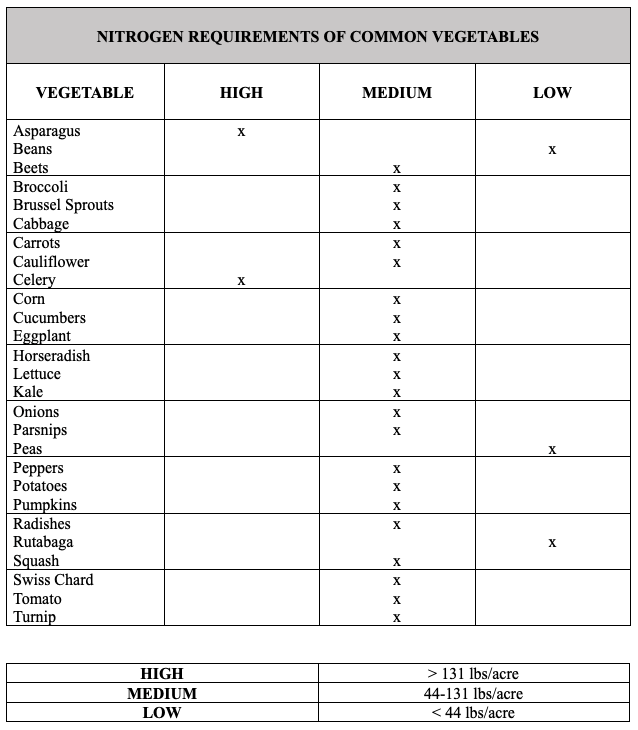
\includegraphics{nitrogen-requirements-veg.png}

}

\caption{\label{fig-nitrogen}Nitrogen Requirements of Vegetables}

\end{figure}

Using your soil's nitrate result from investigation B, what is a plant
you could grow without needing to add any more Nitrogen?

~ ~ ~

\hypertarget{investigation-d-liming-and-base-saturation}{%
\section{INVESTIGATION D: Liming and Base
Saturation}\label{investigation-d-liming-and-base-saturation}}

In the field, quick lime or elemental sulfur is used to adjust pH to a
desired range. The following investigation demonstrates a soil with low
base saturation (Low B.S.) and a soil with high base saturation (High
B.S.) combined with two different amendments. The diagram shows six
variations of soil + solution and the pH for each sample. We used HCl in
place of elemental sulfur. Before recoding the diagram provided in lab,
answer the following questions.

How do you think the quick lime will impact the Low B.S. sample?

~ ~ ~

How will the addition of acid affect the pH in soil with High B.S.?

~ ~ ~

\textbf{Record the pH of each solution here.}

 
  \providecommand{\huxb}[2]{\arrayrulecolor[RGB]{#1}\global\arrayrulewidth=#2pt}
  \providecommand{\huxvb}[2]{\color[RGB]{#1}\vrule width #2pt}
  \providecommand{\huxtpad}[1]{\rule{0pt}{#1}}
  \providecommand{\huxbpad}[1]{\rule[-#1]{0pt}{#1}}

\begin{table}[h!]
\begin{centerbox}
\begin{threeparttable}
 
\setlength{\tabcolsep}{0pt}
\begin{tabularx}{0.9\textwidth}{p{0.45\textwidth} p{0.45\textwidth}}


\hhline{>{\huxb{0, 0, 0}{1}}->{\huxb{0, 0, 0}{1}}-}
\arrayrulecolor{black}

\multicolumn{1}{!{\huxvb{0, 0, 0}{1}}m{0.45\textwidth}!{\huxvb{0, 0, 0}{1}}}{\hspace{0pt}\parbox[c]{0.45\textwidth-0pt-4pt}{\huxtpad{0pt + 1em}\centering \textbf{Type of Solution}\huxbpad{4pt}}} &
\multicolumn{1}{m{0.45\textwidth}!{\huxvb{0, 0, 0}{1}}}{\hspace{4pt}\parbox[c]{0.45\textwidth-4pt-0pt}{\huxtpad{0pt + 1em}\centering \textbf{pH}\huxbpad{4pt}}} \tabularnewline[-0.5pt]


\hhline{>{\huxb{0, 0, 0}{1}}->{\huxb{0, 0, 0}{1}}-}
\arrayrulecolor{black}

\multicolumn{1}{!{\huxvb{0, 0, 0}{1}}m{0.45\textwidth}!{\huxvb{0, 0, 0}{1}}}{\hspace{0pt}\parbox[c]{0.45\textwidth-0pt-4pt}{\huxtpad{20pt + 1em}\centering Low Base Saturation Soil Slurry\huxbpad{20pt}}} &
\multicolumn{1}{m{0.45\textwidth}!{\huxvb{0, 0, 0}{1}}}{\hspace{4pt}\parbox[c]{0.45\textwidth-4pt-0pt}{\huxtpad{20pt + 1em}\centering \huxbpad{20pt}}} \tabularnewline[-0.5pt]


\hhline{>{\huxb{0, 0, 0}{1}}->{\huxb{0, 0, 0}{1}}-}
\arrayrulecolor{black}

\multicolumn{1}{!{\huxvb{0, 0, 0}{1}}m{0.45\textwidth}!{\huxvb{0, 0, 0}{1}}}{\hspace{0pt}\parbox[c]{0.45\textwidth-0pt-4pt}{\huxtpad{20pt + 1em}\centering Low Base Saturation and 1 scoop Lime\huxbpad{20pt}}} &
\multicolumn{1}{m{0.45\textwidth}!{\huxvb{0, 0, 0}{1}}}{\hspace{4pt}\parbox[c]{0.45\textwidth-4pt-0pt}{\huxtpad{20pt + 1em}\centering \huxbpad{20pt}}} \tabularnewline[-0.5pt]


\hhline{>{\huxb{0, 0, 0}{1}}->{\huxb{0, 0, 0}{1}}-}
\arrayrulecolor{black}

\multicolumn{1}{!{\huxvb{0, 0, 0}{1}}m{0.45\textwidth}!{\huxvb{0, 0, 0}{1}}}{\hspace{0pt}\parbox[c]{0.45\textwidth-0pt-4pt}{\huxtpad{20pt + 1em}\centering Low Base Saturation and 10 scoops Lime\huxbpad{20pt}}} &
\multicolumn{1}{m{0.45\textwidth}!{\huxvb{0, 0, 0}{1}}}{\hspace{4pt}\parbox[c]{0.45\textwidth-4pt-0pt}{\huxtpad{20pt + 1em}\centering \huxbpad{20pt}}} \tabularnewline[-0.5pt]


\hhline{>{\huxb{0, 0, 0}{1}}->{\huxb{0, 0, 0}{1}}-}
\arrayrulecolor{black}

\multicolumn{1}{!{\huxvb{0, 0, 0}{1}}m{0.45\textwidth}!{\huxvb{0, 0, 0}{1}}}{\hspace{0pt}\parbox[c]{0.45\textwidth-0pt-4pt}{\huxtpad{20pt + 1em}\centering High Base Saturation Soil Slurry\huxbpad{20pt}}} &
\multicolumn{1}{m{0.45\textwidth}!{\huxvb{0, 0, 0}{1}}}{\hspace{4pt}\parbox[c]{0.45\textwidth-4pt-0pt}{\huxtpad{20pt + 1em}\centering \huxbpad{20pt}}} \tabularnewline[-0.5pt]


\hhline{>{\huxb{0, 0, 0}{1}}->{\huxb{0, 0, 0}{1}}-}
\arrayrulecolor{black}

\multicolumn{1}{!{\huxvb{0, 0, 0}{1}}m{0.45\textwidth}!{\huxvb{0, 0, 0}{1}}}{\hspace{0pt}\parbox[c]{0.45\textwidth-0pt-4pt}{\huxtpad{20pt + 1em}\centering High Base Saturation and 1 mL of 5\% Acid\huxbpad{20pt}}} &
\multicolumn{1}{m{0.45\textwidth}!{\huxvb{0, 0, 0}{1}}}{\hspace{4pt}\parbox[c]{0.45\textwidth-4pt-0pt}{\huxtpad{20pt + 1em}\centering \huxbpad{20pt}}} \tabularnewline[-0.5pt]


\hhline{>{\huxb{0, 0, 0}{1}}->{\huxb{0, 0, 0}{1}}-}
\arrayrulecolor{black}

\multicolumn{1}{!{\huxvb{0, 0, 0}{1}}m{0.45\textwidth}!{\huxvb{0, 0, 0}{1}}}{\hspace{0pt}\parbox[c]{0.45\textwidth-0pt-4pt}{\huxtpad{20pt + 1em}\centering High Base Saturation and 5 mL of 10\% Acid\huxbpad{20pt}}} &
\multicolumn{1}{m{0.45\textwidth}!{\huxvb{0, 0, 0}{1}}}{\hspace{4pt}\parbox[c]{0.45\textwidth-4pt-0pt}{\huxtpad{20pt + 1em}\centering \huxbpad{20pt}}} \tabularnewline[-0.5pt]


\hhline{>{\huxb{0, 0, 0}{1}}->{\huxb{0, 0, 0}{1}}-}
\arrayrulecolor{black}
\end{tabularx}
\end{threeparttable}\par\end{centerbox}

\end{table}
 

Explain the impact on the pH of each soil after the different solutions
were added. Did the results surprise you?

~ ~ ~

\hypertarget{investigation-e-observation-of-plant-nutrient-deficiencies}{%
\section{INVESTIGATION E: Observation of Plant Nutrient
Deficiencies}\label{investigation-e-observation-of-plant-nutrient-deficiencies}}

Nutrient deficiencies in plants can sometimes have complex causes and
symptoms, and can also be related to drought and other types of stress.
Just having a sufficient total amount of an element in the soil does not
always eliminate deficiencies because plant nutrient uptake is dependent
on a wide range of factors including nutrient form, mobility, and soil
properties such as pH, mineralogy, and organic matter. Nutrient
deficiencies can be outwardly manifested in different ways in different
plant species, and the symptoms of some nutrient deficiencies can mimic
other forms of stress. However, experts with enough experience can
diagnose nutrient deficiencies in the field. In this investigation, you
will examine the outward effect of N, P and K deficiencies in corn. Note
that symptoms in other plant species may look similar or may vary,
depending on biology and growth conditions.

Observe and read through examples of nutrient deficiencies in corn.
Then, look at the unknown corn plants with nutrient deficiencies and
determine which particular nutrient is most likely deficient in each
case.

 
  \providecommand{\huxb}[2]{\arrayrulecolor[RGB]{#1}\global\arrayrulewidth=#2pt}
  \providecommand{\huxvb}[2]{\color[RGB]{#1}\vrule width #2pt}
  \providecommand{\huxtpad}[1]{\rule{0pt}{#1}}
  \providecommand{\huxbpad}[1]{\rule[-#1]{0pt}{#1}}

\begin{table}[h!]
\begin{centerbox}
\begin{threeparttable}
 
\setlength{\tabcolsep}{0pt}
\begin{tabularx}{0.9\textwidth}{p{0.45\textwidth} p{0.45\textwidth}}


\hhline{>{\huxb{0, 0, 0}{1}}->{\huxb{0, 0, 0}{1}}-}
\arrayrulecolor{black}

\multicolumn{1}{!{\huxvb{0, 0, 0}{1}}m{0.45\textwidth}!{\huxvb{0, 0, 0}{1}}}{\hspace{0pt}\parbox[c]{0.45\textwidth-0pt-4pt}{\huxtpad{0pt + 1em}\centering \textbf{Unknown Plant}\huxbpad{4pt}}} &
\multicolumn{1}{m{0.45\textwidth}!{\huxvb{0, 0, 0}{1}}}{\hspace{4pt}\parbox[c]{0.45\textwidth-4pt-0pt}{\huxtpad{0pt + 1em}\centering \textbf{Suspected Nutrient Deficiency}\huxbpad{4pt}}} \tabularnewline[-0.5pt]


\hhline{>{\huxb{0, 0, 0}{1}}->{\huxb{0, 0, 0}{1}}-}
\arrayrulecolor{black}

\multicolumn{1}{!{\huxvb{0, 0, 0}{1}}m{0.45\textwidth}!{\huxvb{0, 0, 0}{1}}}{\hspace{0pt}\parbox[c]{0.45\textwidth-0pt-4pt}{\huxtpad{40pt + 1em}\centering 1\huxbpad{40pt}}} &
\multicolumn{1}{m{0.45\textwidth}!{\huxvb{0, 0, 0}{1}}}{\hspace{4pt}\parbox[c]{0.45\textwidth-4pt-0pt}{\huxtpad{40pt + 1em}\centering \huxbpad{40pt}}} \tabularnewline[-0.5pt]


\hhline{>{\huxb{0, 0, 0}{1}}->{\huxb{0, 0, 0}{1}}-}
\arrayrulecolor{black}

\multicolumn{1}{!{\huxvb{0, 0, 0}{1}}m{0.45\textwidth}!{\huxvb{0, 0, 0}{1}}}{\hspace{0pt}\parbox[c]{0.45\textwidth-0pt-4pt}{\huxtpad{40pt + 1em}\centering 2\huxbpad{40pt}}} &
\multicolumn{1}{m{0.45\textwidth}!{\huxvb{0, 0, 0}{1}}}{\hspace{4pt}\parbox[c]{0.45\textwidth-4pt-0pt}{\huxtpad{40pt + 1em}\centering \huxbpad{40pt}}} \tabularnewline[-0.5pt]


\hhline{>{\huxb{0, 0, 0}{1}}->{\huxb{0, 0, 0}{1}}-}
\arrayrulecolor{black}

\multicolumn{1}{!{\huxvb{0, 0, 0}{1}}m{0.45\textwidth}!{\huxvb{0, 0, 0}{1}}}{\hspace{0pt}\parbox[c]{0.45\textwidth-0pt-4pt}{\huxtpad{40pt + 1em}\centering 3\huxbpad{40pt}}} &
\multicolumn{1}{m{0.45\textwidth}!{\huxvb{0, 0, 0}{1}}}{\hspace{4pt}\parbox[c]{0.45\textwidth-4pt-0pt}{\huxtpad{40pt + 1em}\centering \huxbpad{40pt}}} \tabularnewline[-0.5pt]


\hhline{>{\huxb{0, 0, 0}{1}}->{\huxb{0, 0, 0}{1}}-}
\arrayrulecolor{black}
\end{tabularx}
\end{threeparttable}\par\end{centerbox}

\end{table}
 

\hypertarget{investigation-f-common-fertilizer-materials}{%
\section{INVESTIGATION F: Common Fertilizer
Materials}\label{investigation-f-common-fertilizer-materials}}

\textbf{Inorganic Fertilizers}

Plant roots absorb the majority of their nutrients from the soil
solution as simple, inorganic ions (charged atoms or molecules). Larger
molecules can also be absorbed, but their rate of absorption is slow.
Most inorganic fertilizers dissolve readily in water and are immediately
available to plants for uptake. When used according to recommendations,
these types of fertilizers efficiently supply the required nutrients for
plant growth and are safe for the environment. However, excessive rates
can injure plant roots due to high salts and potentially lead to
environmental degradation.

Review the inorganic fertilizers and complete the following table.

 
  \providecommand{\huxb}[2]{\arrayrulecolor[RGB]{#1}\global\arrayrulewidth=#2pt}
  \providecommand{\huxvb}[2]{\color[RGB]{#1}\vrule width #2pt}
  \providecommand{\huxtpad}[1]{\rule{0pt}{#1}}
  \providecommand{\huxbpad}[1]{\rule[-#1]{0pt}{#1}}

\begin{table}[h!]
\begin{centerbox}
\begin{threeparttable}
 
\setlength{\tabcolsep}{0pt}
\begin{tabularx}{0.9\textwidth}{p{0.45\textwidth} p{0.45\textwidth}}


\hhline{>{\huxb{0, 0, 0}{1}}->{\huxb{0, 0, 0}{1}}-}
\arrayrulecolor{black}

\multicolumn{1}{!{\huxvb{0, 0, 0}{1}}m{0.45\textwidth}!{\huxvb{0, 0, 0}{1}}}{\hspace{0pt}\parbox[c]{0.45\textwidth-0pt-4pt}{\huxtpad{0pt + 1em}\centering \textbf{Name of Inorganic Fertilizer}\huxbpad{4pt}}} &
\multicolumn{1}{m{0.45\textwidth}!{\huxvb{0, 0, 0}{1}}}{\hspace{4pt}\parbox[c]{0.45\textwidth-4pt-0pt}{\huxtpad{0pt + 1em}\centering \textbf{Analysis (Grade)}\huxbpad{4pt}}} \tabularnewline[-0.5pt]


\hhline{>{\huxb{0, 0, 0}{1}}->{\huxb{0, 0, 0}{1}}-}
\arrayrulecolor{black}

\multicolumn{1}{!{\huxvb{0, 0, 0}{1}}m{0.45\textwidth}!{\huxvb{0, 0, 0}{1}}}{\hspace{0pt}\parbox[c]{0.45\textwidth-0pt-4pt}{\huxtpad{4pt + 1em}\centering Ammonium nitrate\huxbpad{4pt}}} &
\multicolumn{1}{m{0.45\textwidth}!{\huxvb{0, 0, 0}{1}}}{\hspace{4pt}\parbox[c]{0.45\textwidth-4pt-0pt}{\huxtpad{4pt + 1em}\centering \huxbpad{4pt}}} \tabularnewline[-0.5pt]


\hhline{>{\huxb{0, 0, 0}{1}}->{\huxb{0, 0, 0}{1}}-}
\arrayrulecolor{black}

\multicolumn{1}{!{\huxvb{0, 0, 0}{1}}m{0.45\textwidth}!{\huxvb{0, 0, 0}{1}}}{\hspace{0pt}\parbox[c]{0.45\textwidth-0pt-4pt}{\huxtpad{4pt + 1em}\centering Urea\huxbpad{4pt}}} &
\multicolumn{1}{m{0.45\textwidth}!{\huxvb{0, 0, 0}{1}}}{\hspace{4pt}\parbox[c]{0.45\textwidth-4pt-0pt}{\huxtpad{4pt + 1em}\centering \huxbpad{4pt}}} \tabularnewline[-0.5pt]


\hhline{>{\huxb{0, 0, 0}{1}}->{\huxb{0, 0, 0}{1}}-}
\arrayrulecolor{black}

\multicolumn{1}{!{\huxvb{0, 0, 0}{1}}m{0.45\textwidth}!{\huxvb{0, 0, 0}{1}}}{\hspace{0pt}\parbox[c]{0.45\textwidth-0pt-4pt}{\huxtpad{4pt + 1em}\centering Triple super phosphate\huxbpad{4pt}}} &
\multicolumn{1}{m{0.45\textwidth}!{\huxvb{0, 0, 0}{1}}}{\hspace{4pt}\parbox[c]{0.45\textwidth-4pt-0pt}{\huxtpad{4pt + 1em}\centering \huxbpad{4pt}}} \tabularnewline[-0.5pt]


\hhline{>{\huxb{0, 0, 0}{1}}->{\huxb{0, 0, 0}{1}}-}
\arrayrulecolor{black}

\multicolumn{1}{!{\huxvb{0, 0, 0}{1}}m{0.45\textwidth}!{\huxvb{0, 0, 0}{1}}}{\hspace{0pt}\parbox[c]{0.45\textwidth-0pt-4pt}{\huxtpad{4pt + 1em}\centering Monoammonium phosphate\huxbpad{4pt}}} &
\multicolumn{1}{m{0.45\textwidth}!{\huxvb{0, 0, 0}{1}}}{\hspace{4pt}\parbox[c]{0.45\textwidth-4pt-0pt}{\huxtpad{4pt + 1em}\centering \huxbpad{4pt}}} \tabularnewline[-0.5pt]


\hhline{>{\huxb{0, 0, 0}{1}}->{\huxb{0, 0, 0}{1}}-}
\arrayrulecolor{black}

\multicolumn{1}{!{\huxvb{0, 0, 0}{1}}m{0.45\textwidth}!{\huxvb{0, 0, 0}{1}}}{\hspace{0pt}\parbox[c]{0.45\textwidth-0pt-4pt}{\huxtpad{4pt + 1em}\centering Diammonium phosphate\huxbpad{4pt}}} &
\multicolumn{1}{m{0.45\textwidth}!{\huxvb{0, 0, 0}{1}}}{\hspace{4pt}\parbox[c]{0.45\textwidth-4pt-0pt}{\huxtpad{4pt + 1em}\centering \huxbpad{4pt}}} \tabularnewline[-0.5pt]


\hhline{>{\huxb{0, 0, 0}{1}}->{\huxb{0, 0, 0}{1}}-}
\arrayrulecolor{black}

\multicolumn{1}{!{\huxvb{0, 0, 0}{1}}m{0.45\textwidth}!{\huxvb{0, 0, 0}{1}}}{\hspace{0pt}\parbox[c]{0.45\textwidth-0pt-4pt}{\huxtpad{4pt + 1em}\centering Potassium chloride\huxbpad{0pt}}} &
\multicolumn{1}{m{0.45\textwidth}!{\huxvb{0, 0, 0}{1}}}{\hspace{4pt}\parbox[c]{0.45\textwidth-4pt-0pt}{\huxtpad{4pt + 1em}\centering \huxbpad{0pt}}} \tabularnewline[-0.5pt]


\hhline{>{\huxb{0, 0, 0}{1}}->{\huxb{0, 0, 0}{1}}-}
\arrayrulecolor{black}
\end{tabularx}
\end{threeparttable}\par\end{centerbox}

\end{table}
 

\textbf{Organic Fertilizers}

Organic fertilizers are comprised of a diverse mixture of organic
molecules and usually contain more complex chemical substances that take
time to be broken down into forms usable by plants. These are usually
considered slow-release type fertilizers, compared to the quick-release
characteristics of most inorganic fertilizers. It is important to apply
these organic fertilizers well before periods of rapid plant growth.
Organic fertilizers usually have a low salt index, so larger amounts can
be applied at one time without causing injury to plant roots. With
organic nitrogen sources (except urea), one application can be made
without having to be concerned about losing most of the nitrogen to
leaching. However, even organic fertilizers applied at excessive rates
can cause environmental degradation due to nitrate leaching or runoff of
soluble organic compounds. The cost of organic fertilizers at garden
centers on a per-pound of nutrient basis is usually higher than
quick-release inorganic fertilizers. Manure, compost, and many other
materials used as organic fertilizers add considerable quantities of
organic matter to the soil. Organic matter can increase soil drainage,
aeration, water holding capacity, and the ability of the soil to hold
nutrients. The beneficial effects of organic matter on soil structure
can have a greater effect on plant growth than the fertilizer value of
some of these organic materials. Most organic fertilizers also provide a
variety of macronutrients (besides NPK) as well as many micronutrients.

 
  \providecommand{\huxb}[2]{\arrayrulecolor[RGB]{#1}\global\arrayrulewidth=#2pt}
  \providecommand{\huxvb}[2]{\color[RGB]{#1}\vrule width #2pt}
  \providecommand{\huxtpad}[1]{\rule{0pt}{#1}}
  \providecommand{\huxbpad}[1]{\rule[-#1]{0pt}{#1}}

\begin{table}[h!]
\begin{centerbox}
\begin{threeparttable}
 
\setlength{\tabcolsep}{0pt}
\begin{tabularx}{0.9\textwidth}{p{0.45\textwidth} p{0.45\textwidth}}


\hhline{>{\huxb{0, 0, 0}{1}}->{\huxb{0, 0, 0}{1}}-}
\arrayrulecolor{black}

\multicolumn{1}{!{\huxvb{0, 0, 0}{1}}m{0.45\textwidth}!{\huxvb{0, 0, 0}{1}}}{\hspace{0pt}\parbox[c]{0.45\textwidth-0pt-4pt}{\huxtpad{0pt + 1em}\centering \textbf{Name of Organic Fertilizer}\huxbpad{4pt}}} &
\multicolumn{1}{m{0.45\textwidth}!{\huxvb{0, 0, 0}{1}}}{\hspace{4pt}\parbox[c]{0.45\textwidth-4pt-0pt}{\huxtpad{0pt + 1em}\centering \textbf{Typical Analysis (Grade)- can be variable!}\huxbpad{4pt}}} \tabularnewline[-0.5pt]


\hhline{>{\huxb{0, 0, 0}{1}}->{\huxb{0, 0, 0}{1}}-}
\arrayrulecolor{black}

\multicolumn{1}{!{\huxvb{0, 0, 0}{1}}m{0.45\textwidth}!{\huxvb{0, 0, 0}{1}}}{\hspace{0pt}\parbox[c]{0.45\textwidth-0pt-4pt}{\huxtpad{4pt + 1em}\centering Dairy cattle manure\huxbpad{4pt}}} &
\multicolumn{1}{m{0.45\textwidth}!{\huxvb{0, 0, 0}{1}}}{\hspace{4pt}\parbox[c]{0.45\textwidth-4pt-0pt}{\huxtpad{4pt + 1em}\centering 2-0-2\huxbpad{4pt}}} \tabularnewline[-0.5pt]


\hhline{>{\huxb{0, 0, 0}{1}}->{\huxb{0, 0, 0}{1}}-}
\arrayrulecolor{black}

\multicolumn{1}{!{\huxvb{0, 0, 0}{1}}m{0.45\textwidth}!{\huxvb{0, 0, 0}{1}}}{\hspace{0pt}\parbox[c]{0.45\textwidth-0pt-4pt}{\huxtpad{4pt + 1em}\centering Sheep Manure\huxbpad{4pt}}} &
\multicolumn{1}{m{0.45\textwidth}!{\huxvb{0, 0, 0}{1}}}{\hspace{4pt}\parbox[c]{0.45\textwidth-4pt-0pt}{\huxtpad{4pt + 1em}\centering 2-1-2\huxbpad{4pt}}} \tabularnewline[-0.5pt]


\hhline{>{\huxb{0, 0, 0}{1}}->{\huxb{0, 0, 0}{1}}-}
\arrayrulecolor{black}

\multicolumn{1}{!{\huxvb{0, 0, 0}{1}}m{0.45\textwidth}!{\huxvb{0, 0, 0}{1}}}{\hspace{0pt}\parbox[c]{0.45\textwidth-0pt-4pt}{\huxtpad{4pt + 1em}\centering Poultry manure\huxbpad{4pt}}} &
\multicolumn{1}{m{0.45\textwidth}!{\huxvb{0, 0, 0}{1}}}{\hspace{4pt}\parbox[c]{0.45\textwidth-4pt-0pt}{\huxtpad{4pt + 1em}\centering 4-3-2\huxbpad{4pt}}} \tabularnewline[-0.5pt]


\hhline{>{\huxb{0, 0, 0}{1}}->{\huxb{0, 0, 0}{1}}-}
\arrayrulecolor{black}

\multicolumn{1}{!{\huxvb{0, 0, 0}{1}}m{0.45\textwidth}!{\huxvb{0, 0, 0}{1}}}{\hspace{0pt}\parbox[c]{0.45\textwidth-0pt-4pt}{\huxtpad{4pt + 1em}\centering Seaweed\huxbpad{4pt}}} &
\multicolumn{1}{m{0.45\textwidth}!{\huxvb{0, 0, 0}{1}}}{\hspace{4pt}\parbox[c]{0.45\textwidth-4pt-0pt}{\huxtpad{4pt + 1em}\centering 0-0-1\huxbpad{4pt}}} \tabularnewline[-0.5pt]


\hhline{>{\huxb{0, 0, 0}{1}}->{\huxb{0, 0, 0}{1}}-}
\arrayrulecolor{black}

\multicolumn{1}{!{\huxvb{0, 0, 0}{1}}m{0.45\textwidth}!{\huxvb{0, 0, 0}{1}}}{\hspace{0pt}\parbox[c]{0.45\textwidth-0pt-4pt}{\huxtpad{4pt + 1em}\centering Fish meal\huxbpad{4pt}}} &
\multicolumn{1}{m{0.45\textwidth}!{\huxvb{0, 0, 0}{1}}}{\hspace{4pt}\parbox[c]{0.45\textwidth-4pt-0pt}{\huxtpad{4pt + 1em}\centering 10-6-0\huxbpad{4pt}}} \tabularnewline[-0.5pt]


\hhline{>{\huxb{0, 0, 0}{1}}->{\huxb{0, 0, 0}{1}}-}
\arrayrulecolor{black}

\multicolumn{1}{!{\huxvb{0, 0, 0}{1}}m{0.45\textwidth}!{\huxvb{0, 0, 0}{1}}}{\hspace{0pt}\parbox[c]{0.45\textwidth-0pt-4pt}{\huxtpad{4pt + 1em}\centering Sewage sludge\huxbpad{4pt}}} &
\multicolumn{1}{m{0.45\textwidth}!{\huxvb{0, 0, 0}{1}}}{\hspace{4pt}\parbox[c]{0.45\textwidth-4pt-0pt}{\huxtpad{4pt + 1em}\centering 2-3-0\huxbpad{4pt}}} \tabularnewline[-0.5pt]


\hhline{>{\huxb{0, 0, 0}{1}}->{\huxb{0, 0, 0}{1}}-}
\arrayrulecolor{black}

\multicolumn{1}{!{\huxvb{0, 0, 0}{1}}m{0.45\textwidth}!{\huxvb{0, 0, 0}{1}}}{\hspace{0pt}\parbox[c]{0.45\textwidth-0pt-4pt}{\huxtpad{4pt + 1em}\centering Bone meal\huxbpad{4pt}}} &
\multicolumn{1}{m{0.45\textwidth}!{\huxvb{0, 0, 0}{1}}}{\hspace{4pt}\parbox[c]{0.45\textwidth-4pt-0pt}{\huxtpad{4pt + 1em}\centering 1-12-0\huxbpad{4pt}}} \tabularnewline[-0.5pt]


\hhline{>{\huxb{0, 0, 0}{1}}->{\huxb{0, 0, 0}{1}}-}
\arrayrulecolor{black}

\multicolumn{1}{!{\huxvb{0, 0, 0}{1}}m{0.45\textwidth}!{\huxvb{0, 0, 0}{1}}}{\hspace{0pt}\parbox[c]{0.45\textwidth-0pt-4pt}{\huxtpad{4pt + 1em}\centering Milorganite\huxbpad{0pt}}} &
\multicolumn{1}{m{0.45\textwidth}!{\huxvb{0, 0, 0}{1}}}{\hspace{4pt}\parbox[c]{0.45\textwidth-4pt-0pt}{\huxtpad{4pt + 1em}\centering 6-3-0\huxbpad{0pt}}} \tabularnewline[-0.5pt]


\hhline{>{\huxb{0, 0, 0}{1}}->{\huxb{0, 0, 0}{1}}-}
\arrayrulecolor{black}
\end{tabularx}
\end{threeparttable}\par\end{centerbox}

\end{table}
 

Complete the table below. For each situation described, decide which
form of fertilizer would be preferred, inorganic or organic. Make an X
in the appropriate box.

 
  \providecommand{\huxb}[2]{\arrayrulecolor[RGB]{#1}\global\arrayrulewidth=#2pt}
  \providecommand{\huxvb}[2]{\color[RGB]{#1}\vrule width #2pt}
  \providecommand{\huxtpad}[1]{\rule{0pt}{#1}}
  \providecommand{\huxbpad}[1]{\rule[-#1]{0pt}{#1}}

\begin{table}[h!]
\begin{centerbox}
\begin{threeparttable}
 
\setlength{\tabcolsep}{0pt}
\begin{tabularx}{0.9\textwidth}{p{0.3\textwidth} p{0.3\textwidth} p{0.3\textwidth}}


\hhline{>{\huxb{0, 0, 0}{1}}->{\huxb{0, 0, 0}{1}}->{\huxb{0, 0, 0}{1}}-}
\arrayrulecolor{black}

\multicolumn{1}{!{\huxvb{0, 0, 0}{1}}m{0.3\textwidth}!{\huxvb{0, 0, 0}{1}}}{\hspace{0pt}\parbox[c]{0.3\textwidth-0pt-4pt}{\huxtpad{0pt + 1em}\centering \textbf{Situation}\huxbpad{4pt}}} &
\multicolumn{1}{m{0.3\textwidth}!{\huxvb{0, 0, 0}{1}}}{\hspace{4pt}\parbox[c]{0.3\textwidth-4pt-4pt}{\huxtpad{0pt + 1em}\centering \textbf{Preferred form: Inorganic}\huxbpad{4pt}}} &
\multicolumn{1}{m{0.3\textwidth}!{\huxvb{0, 0, 0}{1}}}{\hspace{4pt}\parbox[c]{0.3\textwidth-4pt-0pt}{\huxtpad{0pt + 1em}\centering \textbf{Preferred form: Organic}\huxbpad{4pt}}} \tabularnewline[-0.5pt]


\hhline{>{\huxb{0, 0, 0}{1}}->{\huxb{0, 0, 0}{1}}->{\huxb{0, 0, 0}{1}}-}
\arrayrulecolor{black}

\multicolumn{1}{!{\huxvb{0, 0, 0}{1}}m{0.3\textwidth}!{\huxvb{0, 0, 0}{1}}}{\hspace{0pt}\parbox[c]{0.3\textwidth-0pt-4pt}{\huxtpad{4pt + 1em}\centering Need to make nutrients quickly available to plants \huxbpad{4pt}}} &
\multicolumn{1}{m{0.3\textwidth}!{\huxvb{0, 0, 0}{1}}}{\hspace{4pt}\parbox[c]{0.3\textwidth-4pt-4pt}{\huxtpad{4pt + 1em}\centering \huxbpad{4pt}}} &
\multicolumn{1}{m{0.3\textwidth}!{\huxvb{0, 0, 0}{1}}}{\hspace{4pt}\parbox[c]{0.3\textwidth-4pt-0pt}{\huxtpad{4pt + 1em}\centering \huxbpad{4pt}}} \tabularnewline[-0.5pt]


\hhline{>{\huxb{0, 0, 0}{1}}->{\huxb{0, 0, 0}{1}}->{\huxb{0, 0, 0}{1}}-}
\arrayrulecolor{black}

\multicolumn{1}{!{\huxvb{0, 0, 0}{1}}m{0.3\textwidth}!{\huxvb{0, 0, 0}{1}}}{\hspace{0pt}\parbox[c]{0.3\textwidth-0pt-4pt}{\huxtpad{4pt + 1em}\centering Desire to minimize fertilizer cost\huxbpad{4pt}}} &
\multicolumn{1}{m{0.3\textwidth}!{\huxvb{0, 0, 0}{1}}}{\hspace{4pt}\parbox[c]{0.3\textwidth-4pt-4pt}{\huxtpad{4pt + 1em}\centering \huxbpad{4pt}}} &
\multicolumn{1}{m{0.3\textwidth}!{\huxvb{0, 0, 0}{1}}}{\hspace{4pt}\parbox[c]{0.3\textwidth-4pt-0pt}{\huxtpad{4pt + 1em}\centering \huxbpad{4pt}}} \tabularnewline[-0.5pt]


\hhline{>{\huxb{0, 0, 0}{1}}->{\huxb{0, 0, 0}{1}}->{\huxb{0, 0, 0}{1}}-}
\arrayrulecolor{black}

\multicolumn{1}{!{\huxvb{0, 0, 0}{1}}m{0.3\textwidth}!{\huxvb{0, 0, 0}{1}}}{\hspace{0pt}\parbox[c]{0.3\textwidth-0pt-4pt}{\huxtpad{4pt + 1em}\centering Concerned about increasing the salt content in the soil\huxbpad{4pt}}} &
\multicolumn{1}{m{0.3\textwidth}!{\huxvb{0, 0, 0}{1}}}{\hspace{4pt}\parbox[c]{0.3\textwidth-4pt-4pt}{\huxtpad{4pt + 1em}\centering \huxbpad{4pt}}} &
\multicolumn{1}{m{0.3\textwidth}!{\huxvb{0, 0, 0}{1}}}{\hspace{4pt}\parbox[c]{0.3\textwidth-4pt-0pt}{\huxtpad{4pt + 1em}\centering \huxbpad{4pt}}} \tabularnewline[-0.5pt]


\hhline{>{\huxb{0, 0, 0}{1}}->{\huxb{0, 0, 0}{1}}->{\huxb{0, 0, 0}{1}}-}
\arrayrulecolor{black}

\multicolumn{1}{!{\huxvb{0, 0, 0}{1}}m{0.3\textwidth}!{\huxvb{0, 0, 0}{1}}}{\hspace{0pt}\parbox[c]{0.3\textwidth-0pt-4pt}{\huxtpad{4pt + 1em}\centering Need to improve soil structure\huxbpad{4pt}}} &
\multicolumn{1}{m{0.3\textwidth}!{\huxvb{0, 0, 0}{1}}}{\hspace{4pt}\parbox[c]{0.3\textwidth-4pt-4pt}{\huxtpad{4pt + 1em}\centering \huxbpad{4pt}}} &
\multicolumn{1}{m{0.3\textwidth}!{\huxvb{0, 0, 0}{1}}}{\hspace{4pt}\parbox[c]{0.3\textwidth-4pt-0pt}{\huxtpad{4pt + 1em}\centering \huxbpad{4pt}}} \tabularnewline[-0.5pt]


\hhline{>{\huxb{0, 0, 0}{1}}->{\huxb{0, 0, 0}{1}}->{\huxb{0, 0, 0}{1}}-}
\arrayrulecolor{black}

\multicolumn{1}{!{\huxvb{0, 0, 0}{1}}m{0.3\textwidth}!{\huxvb{0, 0, 0}{1}}}{\hspace{0pt}\parbox[c]{0.3\textwidth-0pt-4pt}{\huxtpad{4pt + 1em}\centering Minimize nitrate leaching into groundwater\huxbpad{4pt}}} &
\multicolumn{1}{m{0.3\textwidth}!{\huxvb{0, 0, 0}{1}}}{\hspace{4pt}\parbox[c]{0.3\textwidth-4pt-4pt}{\huxtpad{4pt + 1em}\centering \huxbpad{4pt}}} &
\multicolumn{1}{m{0.3\textwidth}!{\huxvb{0, 0, 0}{1}}}{\hspace{4pt}\parbox[c]{0.3\textwidth-4pt-0pt}{\huxtpad{4pt + 1em}\centering \huxbpad{4pt}}} \tabularnewline[-0.5pt]


\hhline{>{\huxb{0, 0, 0}{1}}->{\huxb{0, 0, 0}{1}}->{\huxb{0, 0, 0}{1}}-}
\arrayrulecolor{black}

\multicolumn{1}{!{\huxvb{0, 0, 0}{1}}m{0.3\textwidth}!{\huxvb{0, 0, 0}{1}}}{\hspace{0pt}\parbox[c]{0.3\textwidth-0pt-4pt}{\huxtpad{4pt + 1em}\centering Want to provide only one or two nutrients per application\huxbpad{0pt}}} &
\multicolumn{1}{m{0.3\textwidth}!{\huxvb{0, 0, 0}{1}}}{\hspace{4pt}\parbox[c]{0.3\textwidth-4pt-4pt}{\huxtpad{4pt + 1em}\centering \huxbpad{0pt}}} &
\multicolumn{1}{m{0.3\textwidth}!{\huxvb{0, 0, 0}{1}}}{\hspace{4pt}\parbox[c]{0.3\textwidth-4pt-0pt}{\huxtpad{4pt + 1em}\centering \huxbpad{0pt}}} \tabularnewline[-0.5pt]


\hhline{>{\huxb{0, 0, 0}{1}}->{\huxb{0, 0, 0}{1}}->{\huxb{0, 0, 0}{1}}-}
\arrayrulecolor{black}
\end{tabularx}
\end{threeparttable}\par\end{centerbox}

\end{table}
 

\hypertarget{investigation-g-reading-and-using-a-soil-test-report}{%
\section{INVESTIGATION G: Reading and Using a Soil Test
Report}\label{investigation-g-reading-and-using-a-soil-test-report}}

Soil testing is a useful nutrient management tool. If used in a
predictive mode, a soil test can reduce the environmental risks from the
addition of nutrients to the soil while optimizing plant growth. There
are two soil reports from the soil we observed in the field last week on
the bench. One has soil test results and recommendations for a lawn and
garden, while the other report is for future farm and field planting.
Fill in the following table of each soil test. Note that recommendations
are in P2O5 and K2O, so there is no need to convert. Use the farm and
field report to make a recommendation for planting corn or grain.

 
  \providecommand{\huxb}[2]{\arrayrulecolor[RGB]{#1}\global\arrayrulewidth=#2pt}
  \providecommand{\huxvb}[2]{\color[RGB]{#1}\vrule width #2pt}
  \providecommand{\huxtpad}[1]{\rule{0pt}{#1}}
  \providecommand{\huxbpad}[1]{\rule[-#1]{0pt}{#1}}

\begin{table}[h!]
\begin{centerbox}
\begin{threeparttable}
 
\setlength{\tabcolsep}{0pt}
\begin{tabularx}{0.9\textwidth}{p{0.3\textwidth} p{0.3\textwidth} p{0.3\textwidth}}


\hhline{>{\huxb{0, 0, 0}{1}}->{\huxb{0, 0, 0}{1}}->{\huxb{0, 0, 0}{1}}-}
\arrayrulecolor{black}

\multicolumn{1}{!{\huxvb{0, 0, 0}{1}}m{0.3\textwidth}!{\huxvb{0, 0, 0}{1}}}{\hspace{0pt}\parbox[c]{0.3\textwidth-0pt-4pt}{\huxtpad{0pt + 1em}\centering \textbf{Question}\huxbpad{4pt}}} &
\multicolumn{1}{m{0.3\textwidth}!{\huxvb{0, 0, 0}{1}}}{\hspace{4pt}\parbox[c]{0.3\textwidth-4pt-4pt}{\huxtpad{0pt + 1em}\centering \textbf{Lawn \& Garden Report}\huxbpad{4pt}}} &
\multicolumn{1}{m{0.3\textwidth}!{\huxvb{0, 0, 0}{1}}}{\hspace{4pt}\parbox[c]{0.3\textwidth-4pt-0pt}{\huxtpad{0pt + 1em}\centering \textbf{Farm \& Field Report}\huxbpad{4pt}}} \tabularnewline[-0.5pt]


\hhline{>{\huxb{0, 0, 0}{1}}->{\huxb{0, 0, 0}{1}}->{\huxb{0, 0, 0}{1}}-}
\arrayrulecolor{black}

\multicolumn{1}{!{\huxvb{0, 0, 0}{1}}m{0.3\textwidth}!{\huxvb{0, 0, 0}{1}}}{\hspace{0pt}\parbox[c]{0.3\textwidth-0pt-4pt}{\huxtpad{4pt + 1em}\centering What is the pH of the soil?\huxbpad{4pt}}} &
\multicolumn{1}{m{0.3\textwidth}!{\huxvb{0, 0, 0}{1}}}{\hspace{4pt}\parbox[c]{0.3\textwidth-4pt-4pt}{\huxtpad{4pt + 1em}\centering \huxbpad{4pt}}} &
\multicolumn{1}{m{0.3\textwidth}!{\huxvb{0, 0, 0}{1}}}{\hspace{4pt}\parbox[c]{0.3\textwidth-4pt-0pt}{\huxtpad{4pt + 1em}\centering \huxbpad{4pt}}} \tabularnewline[-0.5pt]


\hhline{>{\huxb{0, 0, 0}{1}}->{\huxb{0, 0, 0}{1}}->{\huxb{0, 0, 0}{1}}-}
\arrayrulecolor{black}

\multicolumn{1}{!{\huxvb{0, 0, 0}{1}}m{0.3\textwidth}!{\huxvb{0, 0, 0}{1}}}{\hspace{0pt}\parbox[c]{0.3\textwidth-0pt-4pt}{\huxtpad{4pt + 1em}\centering What is the estimated soil texture?\huxbpad{4pt}}} &
\multicolumn{1}{m{0.3\textwidth}!{\huxvb{0, 0, 0}{1}}}{\hspace{4pt}\parbox[c]{0.3\textwidth-4pt-4pt}{\huxtpad{4pt + 1em}\centering \huxbpad{4pt}}} &
\multicolumn{1}{m{0.3\textwidth}!{\huxvb{0, 0, 0}{1}}}{\hspace{4pt}\parbox[c]{0.3\textwidth-4pt-0pt}{\huxtpad{4pt + 1em}\centering \huxbpad{4pt}}} \tabularnewline[-0.5pt]


\hhline{>{\huxb{0, 0, 0}{1}}->{\huxb{0, 0, 0}{1}}->{\huxb{0, 0, 0}{1}}-}
\arrayrulecolor{black}

\multicolumn{1}{!{\huxvb{0, 0, 0}{1}}m{0.3\textwidth}!{\huxvb{0, 0, 0}{1}}}{\hspace{0pt}\parbox[c]{0.3\textwidth-0pt-4pt}{\huxtpad{4pt + 1em}\centering Was the soil test for P Bray or Olsen?\huxbpad{4pt}}} &
\multicolumn{1}{m{0.3\textwidth}!{\huxvb{0, 0, 0}{1}}}{\hspace{4pt}\parbox[c]{0.3\textwidth-4pt-4pt}{\huxtpad{4pt + 1em}\centering \huxbpad{4pt}}} &
\multicolumn{1}{m{0.3\textwidth}!{\huxvb{0, 0, 0}{1}}}{\hspace{4pt}\parbox[c]{0.3\textwidth-4pt-0pt}{\huxtpad{4pt + 1em}\centering \huxbpad{4pt}}} \tabularnewline[-0.5pt]


\hhline{>{\huxb{0, 0, 0}{1}}->{\huxb{0, 0, 0}{1}}->{\huxb{0, 0, 0}{1}}-}
\arrayrulecolor{black}

\multicolumn{1}{!{\huxvb{0, 0, 0}{1}}m{0.3\textwidth}!{\huxvb{0, 0, 0}{1}}}{\hspace{0pt}\parbox[c]{0.3\textwidth-0pt-4pt}{\huxtpad{4pt + 1em}\centering Why was that particular method chosen? (see lecture 4-4 slide 7)\huxbpad{4pt}}} &
\multicolumn{1}{m{0.3\textwidth}!{\huxvb{0, 0, 0}{1}}}{\hspace{4pt}\parbox[c]{0.3\textwidth-4pt-4pt}{\huxtpad{4pt + 1em}\centering \huxbpad{4pt}}} &
\multicolumn{1}{m{0.3\textwidth}!{\huxvb{0, 0, 0}{1}}}{\hspace{4pt}\parbox[c]{0.3\textwidth-4pt-0pt}{\huxtpad{4pt + 1em}\centering \huxbpad{4pt}}} \tabularnewline[-0.5pt]


\hhline{>{\huxb{0, 0, 0}{1}}->{\huxb{0, 0, 0}{1}}->{\huxb{0, 0, 0}{1}}-}
\arrayrulecolor{black}

\multicolumn{1}{!{\huxvb{0, 0, 0}{1}}m{0.3\textwidth}!{\huxvb{0, 0, 0}{1}}}{\hspace{0pt}\parbox[c]{0.3\textwidth-0pt-4pt}{\huxtpad{4pt + 1em}\centering What is the K soil test result? (ppm)\huxbpad{4pt}}} &
\multicolumn{1}{m{0.3\textwidth}!{\huxvb{0, 0, 0}{1}}}{\hspace{4pt}\parbox[c]{0.3\textwidth-4pt-4pt}{\huxtpad{4pt + 1em}\centering \huxbpad{4pt}}} &
\multicolumn{1}{m{0.3\textwidth}!{\huxvb{0, 0, 0}{1}}}{\hspace{4pt}\parbox[c]{0.3\textwidth-4pt-0pt}{\huxtpad{4pt + 1em}\centering \huxbpad{4pt}}} \tabularnewline[-0.5pt]


\hhline{>{\huxb{0, 0, 0}{1}}->{\huxb{0, 0, 0}{1}}->{\huxb{0, 0, 0}{1}}-}
\arrayrulecolor{black}

\multicolumn{1}{!{\huxvb{0, 0, 0}{1}}m{0.3\textwidth}!{\huxvb{0, 0, 0}{1}}}{\hspace{0pt}\parbox[c]{0.3\textwidth-0pt-4pt}{\huxtpad{4pt + 1em}\centering What is the nitrogen (N) recommendation?\huxbpad{4pt}}} &
\multicolumn{1}{m{0.3\textwidth}!{\huxvb{0, 0, 0}{1}}}{\hspace{4pt}\parbox[c]{0.3\textwidth-4pt-4pt}{\huxtpad{4pt + 1em}\raggedleft lb N/1000 sq ft\huxbpad{4pt}}} &
\multicolumn{1}{m{0.3\textwidth}!{\huxvb{0, 0, 0}{1}}}{\hspace{4pt}\parbox[c]{0.3\textwidth-4pt-0pt}{\huxtpad{4pt + 1em}\raggedleft lb N/acre\huxbpad{4pt}}} \tabularnewline[-0.5pt]


\hhline{>{\huxb{0, 0, 0}{1}}->{\huxb{0, 0, 0}{1}}->{\huxb{0, 0, 0}{1}}-}
\arrayrulecolor{black}

\multicolumn{1}{!{\huxvb{0, 0, 0}{1}}m{0.3\textwidth}!{\huxvb{0, 0, 0}{1}}}{\hspace{0pt}\parbox[c]{0.3\textwidth-0pt-4pt}{\huxtpad{4pt + 1em}\centering What is the phosphate (P) recommendation?\huxbpad{4pt}}} &
\multicolumn{1}{m{0.3\textwidth}!{\huxvb{0, 0, 0}{1}}}{\hspace{4pt}\parbox[c]{0.3\textwidth-4pt-4pt}{\huxtpad{4pt + 1em}\raggedleft lb P2O5 /1000 sq ft\huxbpad{4pt}}} &
\multicolumn{1}{m{0.3\textwidth}!{\huxvb{0, 0, 0}{1}}}{\hspace{4pt}\parbox[c]{0.3\textwidth-4pt-0pt}{\huxtpad{4pt + 1em}\raggedleft lb P2O5/acre\huxbpad{4pt}}} \tabularnewline[-0.5pt]


\hhline{>{\huxb{0, 0, 0}{1}}->{\huxb{0, 0, 0}{1}}->{\huxb{0, 0, 0}{1}}-}
\arrayrulecolor{black}

\multicolumn{1}{!{\huxvb{0, 0, 0}{1}}m{0.3\textwidth}!{\huxvb{0, 0, 0}{1}}}{\hspace{0pt}\parbox[c]{0.3\textwidth-0pt-4pt}{\huxtpad{4pt + 1em}\centering What is the potash (K) recommendation?\huxbpad{0pt}}} &
\multicolumn{1}{m{0.3\textwidth}!{\huxvb{0, 0, 0}{1}}}{\hspace{4pt}\parbox[c]{0.3\textwidth-4pt-4pt}{\huxtpad{4pt + 1em}\raggedleft lb K2O/1000 sq ft\huxbpad{0pt}}} &
\multicolumn{1}{m{0.3\textwidth}!{\huxvb{0, 0, 0}{1}}}{\hspace{4pt}\parbox[c]{0.3\textwidth-4pt-0pt}{\huxtpad{4pt + 1em}\raggedleft lb K2O/acre\huxbpad{0pt}}} \tabularnewline[-0.5pt]


\hhline{>{\huxb{0, 0, 0}{1}}->{\huxb{0, 0, 0}{1}}->{\huxb{0, 0, 0}{1}}-}
\arrayrulecolor{black}
\end{tabularx}
\end{threeparttable}\par\end{centerbox}

\end{table}
 

\bookmarksetup{startatroot}

\hypertarget{soil-management-physical}{%
\chapter{\texorpdfstring{\textbf{Soil Management:
Physical}}{Soil Management: Physical}}\label{soil-management-physical}}

\begin{tcolorbox}[enhanced jigsaw, colframe=quarto-callout-note-color-frame, coltitle=black, arc=.35mm, breakable, bottomrule=.15mm, colback=white, rightrule=.15mm, toprule=.15mm, opacityback=0, bottomtitle=1mm, left=2mm, titlerule=0mm, leftrule=.75mm, opacitybacktitle=0.6, toptitle=1mm, title=\textcolor{quarto-callout-note-color}{\faInfo}\hspace{0.5em}{Objectives}, colbacktitle=quarto-callout-note-color!10!white]

\begin{itemize}
\tightlist
\item
  Learn how to use the Universal Soil Loss Equation, USLE.
\item
  Determine the effect of crop management and cropping practices on soil
  loss.
\end{itemize}

\end{tcolorbox}

\begin{tcolorbox}[enhanced jigsaw, colframe=quarto-callout-tip-color-frame, coltitle=black, arc=.35mm, breakable, bottomrule=.15mm, colback=white, rightrule=.15mm, toprule=.15mm, opacityback=0, bottomtitle=1mm, left=2mm, titlerule=0mm, leftrule=.75mm, opacitybacktitle=0.6, toptitle=1mm, title=\textcolor{quarto-callout-tip-color}{\faLightbulb}\hspace{0.5em}{Key Words \& Concepts}, colbacktitle=quarto-callout-tip-color!10!white]

\begin{itemize}
\tightlist
\item
  USLE
\item
  T
\item
  Conservation tillage
\item
  Conventional tillage
\item
  Crop management
\item
  Cropping practice
\end{itemize}

\end{tcolorbox}

\hypertarget{investigation-a-soil-water-erosion-raindrop-impact}{%
\section{INVESTIGATION A: Soil Water Erosion: Raindrop
Impact}\label{investigation-a-soil-water-erosion-raindrop-impact}}

Soil erosion occurs naturally on all land. Soil erosion may proceed
relatively unnoticed or it may occur at an alarming rate --- causing
serious loss of topsoil. The loss of soil from farmlands is usually
reflected in reduced crop production potential, lower surface water
quality and damaged drainage networks.

\textbf{Raindrop Impact}

Spread a thin layer of each soil on separate pieces of paper. Hold the
water dropper one foot above the surface of the soil-covered paper.
Allow a single drop of water to fall from the dropper onto the soil.
Observe the effects on the silty and sandy soils.

\begin{enumerate}
\def\labelenumi{\arabic{enumi}.}
\tightlist
\item
  What effect does the impact of the water have on each soil (explain
  any differences that you observe)?
\end{enumerate}

~ ~ ~

\begin{enumerate}
\def\labelenumi{\arabic{enumi}.}
\setcounter{enumi}{1}
\tightlist
\item
  How would the presence of plant cover change this?
\end{enumerate}

~ ~ ~

\hypertarget{investigation-b-soil-water-erosion-residue-cover-and-runoff}{%
\section{INVESTIGATION B: Soil Water Erosion: Residue Cover and
Runoff}\label{investigation-b-soil-water-erosion-residue-cover-and-runoff}}

\textbf{Water Runoff}

Pour just enough water (about ½ of the small beaker) into each funnel at
the top of each column so that a small amount of water runs off the soil
surface and collects in a larger beaker. Compare the difference in
erosion between the uncovered and covered soil. Complete the following
table.

 
  \providecommand{\huxb}[2]{\arrayrulecolor[RGB]{#1}\global\arrayrulewidth=#2pt}
  \providecommand{\huxvb}[2]{\color[RGB]{#1}\vrule width #2pt}
  \providecommand{\huxtpad}[1]{\rule{0pt}{#1}}
  \providecommand{\huxbpad}[1]{\rule[-#1]{0pt}{#1}}

\begin{table}[h!]
\begin{centerbox}
\begin{threeparttable}
 
\setlength{\tabcolsep}{0pt}
\begin{tabularx}{0.9\textwidth}{p{0.3\textwidth} p{0.3\textwidth} p{0.3\textwidth}}


\hhline{>{\huxb{0, 0, 0}{1}}->{\huxb{0, 0, 0}{1}}->{\huxb{0, 0, 0}{1}}-}
\arrayrulecolor{black}

\multicolumn{1}{!{\huxvb{0, 0, 0}{1}}m{0.3\textwidth}!{\huxvb{0, 0, 0}{1}}}{\hspace{0pt}\parbox[c]{0.3\textwidth-0pt-4pt}{\huxtpad{0pt + 1em}\centering \textbf{Soil}\huxbpad{4pt}}} &
\multicolumn{1}{m{0.3\textwidth}!{\huxvb{0, 0, 0}{1}}}{\hspace{4pt}\parbox[c]{0.3\textwidth-4pt-4pt}{\huxtpad{0pt + 1em}\centering \textbf{Rate (High/Low)}\huxbpad{4pt}}} &
\multicolumn{1}{m{0.3\textwidth}!{\huxvb{0, 0, 0}{1}}}{\hspace{4pt}\parbox[c]{0.3\textwidth-4pt-0pt}{\huxtpad{0pt + 1em}\centering \textbf{Explanation}\huxbpad{4pt}}} \tabularnewline[-0.5pt]


\hhline{>{\huxb{0, 0, 0}{1}}->{\huxb{0, 0, 0}{1}}->{\huxb{0, 0, 0}{1}}-}
\arrayrulecolor{black}

\multicolumn{1}{!{\huxvb{0, 0, 0}{1}}m{0.3\textwidth}!{\huxvb{0, 0, 0}{1}}}{\hspace{0pt}\parbox[c]{0.3\textwidth-0pt-4pt}{\huxtpad{30pt + 1em}\centering Uncovered\huxbpad{30pt}}} &
\multicolumn{1}{m{0.3\textwidth}!{\huxvb{0, 0, 0}{1}}}{\hspace{4pt}\parbox[c]{0.3\textwidth-4pt-4pt}{\huxtpad{30pt + 1em}\centering \huxbpad{30pt}}} &
\multicolumn{1}{m{0.3\textwidth}!{\huxvb{0, 0, 0}{1}}}{\hspace{4pt}\parbox[c]{0.3\textwidth-4pt-0pt}{\huxtpad{30pt + 1em}\centering \huxbpad{30pt}}} \tabularnewline[-0.5pt]


\hhline{>{\huxb{0, 0, 0}{1}}->{\huxb{0, 0, 0}{1}}->{\huxb{0, 0, 0}{1}}-}
\arrayrulecolor{black}

\multicolumn{1}{!{\huxvb{0, 0, 0}{1}}m{0.3\textwidth}!{\huxvb{0, 0, 0}{1}}}{\hspace{0pt}\parbox[c]{0.3\textwidth-0pt-4pt}{\huxtpad{30pt + 1em}\centering Covered\huxbpad{30pt}}} &
\multicolumn{1}{m{0.3\textwidth}!{\huxvb{0, 0, 0}{1}}}{\hspace{4pt}\parbox[c]{0.3\textwidth-4pt-4pt}{\huxtpad{30pt + 1em}\centering \huxbpad{30pt}}} &
\multicolumn{1}{m{0.3\textwidth}!{\huxvb{0, 0, 0}{1}}}{\hspace{4pt}\parbox[c]{0.3\textwidth-4pt-0pt}{\huxtpad{30pt + 1em}\centering \huxbpad{30pt}}} \tabularnewline[-0.5pt]


\hhline{>{\huxb{0, 0, 0}{1}}->{\huxb{0, 0, 0}{1}}->{\huxb{0, 0, 0}{1}}-}
\arrayrulecolor{black}
\end{tabularx}
\end{threeparttable}\par\end{centerbox}

\end{table}
 

\hypertarget{investigation-c-predicting-erosion-with-the-universal-soil-loss-equation}{%
\section{INVESTIGATION C: Predicting Erosion with the Universal Soil
Loss
Equation}\label{investigation-c-predicting-erosion-with-the-universal-soil-loss-equation}}

Determine the erosion rates for the Seaton and Frontenac soils (located
on the plaster landscape model). Use the white-painted lines and
indicated lengths for the LS factor for the three erosion estimates.
These soils are located in Winona County, MN.

\[
USLE:\ A\ =\ R\ *\ K\ *\ LS\ *\ C\ *\ P
\]

A = Soil loss in tons per acre

R = Rainfall factor

C = Crop management factor

K = Soil erodibility factor (use surface values)

LS = Slope length and slope steepness factor

P = Erosion control practice factor

T = Tolerable loss

Complete the table below following steps 1 -- 5.

 
  \providecommand{\huxb}[2]{\arrayrulecolor[RGB]{#1}\global\arrayrulewidth=#2pt}
  \providecommand{\huxvb}[2]{\color[RGB]{#1}\vrule width #2pt}
  \providecommand{\huxtpad}[1]{\rule{0pt}{#1}}
  \providecommand{\huxbpad}[1]{\rule[-#1]{0pt}{#1}}

\begin{table}[h!]
\begin{centerbox}
\begin{threeparttable}
 
\setlength{\tabcolsep}{0pt}
\begin{tabularx}{0.9\textwidth}{p{0.1125\textwidth} p{0.1125\textwidth} p{0.1125\textwidth} p{0.1125\textwidth} p{0.1125\textwidth} p{0.1125\textwidth} p{0.1125\textwidth} p{0.1125\textwidth}}


\hhline{>{\huxb{0, 0, 0}{1}}->{\huxb{0, 0, 0}{1}}->{\huxb{0, 0, 0}{1}}->{\huxb{0, 0, 0}{1}}->{\huxb{0, 0, 0}{1}}->{\huxb{0, 0, 0}{1}}->{\huxb{0, 0, 0}{1}}->{\huxb{0, 0, 0}{1}}-}
\arrayrulecolor{black}

\multicolumn{1}{!{\huxvb{0, 0, 0}{1}}m{0.1125\textwidth}!{\huxvb{0, 0, 0}{1}}}{\hspace{0pt}\parbox[c]{0.1125\textwidth-0pt-4pt}{\huxtpad{0pt + 1em}\centering \textbf{}\huxbpad{4pt}}} &
\multicolumn{1}{m{0.1125\textwidth}!{\huxvb{0, 0, 0}{1}}}{\hspace{4pt}\parbox[c]{0.1125\textwidth-4pt-4pt}{\huxtpad{0pt + 1em}\centering \textbf{R}\huxbpad{4pt}}} &
\multicolumn{1}{m{0.1125\textwidth}!{\huxvb{0, 0, 0}{1}}}{\hspace{4pt}\parbox[c]{0.1125\textwidth-4pt-4pt}{\huxtpad{0pt + 1em}\centering \textbf{K}\huxbpad{4pt}}} &
\multicolumn{1}{m{0.1125\textwidth}!{\huxvb{0, 0, 0}{1}}}{\hspace{4pt}\parbox[c]{0.1125\textwidth-4pt-4pt}{\huxtpad{0pt + 1em}\centering \textbf{LS}\huxbpad{4pt}}} &
\multicolumn{1}{m{0.1125\textwidth}!{\huxvb{0, 0, 0}{1}}}{\hspace{4pt}\parbox[c]{0.1125\textwidth-4pt-4pt}{\huxtpad{0pt + 1em}\centering \textbf{C}\huxbpad{4pt}}} &
\multicolumn{1}{m{0.1125\textwidth}!{\huxvb{0, 0, 0}{1}}}{\hspace{4pt}\parbox[c]{0.1125\textwidth-4pt-4pt}{\huxtpad{0pt + 1em}\centering \textbf{P}\huxbpad{4pt}}} &
\multicolumn{1}{m{0.1125\textwidth}!{\huxvb{0, 0, 0}{1}}}{\hspace{4pt}\parbox[c]{0.1125\textwidth-4pt-4pt}{\huxtpad{0pt + 1em}\centering \textbf{A}\huxbpad{4pt}}} &
\multicolumn{1}{m{0.1125\textwidth}!{\huxvb{0, 0, 0}{1}}}{\hspace{4pt}\parbox[c]{0.1125\textwidth-4pt-0pt}{\huxtpad{0pt + 1em}\centering \textbf{T}\huxbpad{4pt}}} \tabularnewline[-0.5pt]


\hhline{>{\huxb{0, 0, 0}{1}}->{\huxb{0, 0, 0}{1}}->{\huxb{0, 0, 0}{1}}->{\huxb{0, 0, 0}{1}}->{\huxb{0, 0, 0}{1}}->{\huxb{0, 0, 0}{1}}->{\huxb{0, 0, 0}{1}}->{\huxb{0, 0, 0}{1}}-}
\arrayrulecolor{black}

\multicolumn{1}{!{\huxvb{0, 0, 0}{1}}m{0.1125\textwidth}!{\huxvb{0, 0, 0}{1}}}{\hspace{0pt}\parbox[c]{0.1125\textwidth-0pt-4pt}{\huxtpad{4pt + 1em}\centering Site 1: Corn-oats-pasture rotation; no conservation practices\huxbpad{4pt}}} &
\multicolumn{1}{m{0.1125\textwidth}!{\huxvb{0, 0, 0}{1}}}{\hspace{4pt}\parbox[c]{0.1125\textwidth-4pt-4pt}{\huxtpad{4pt + 1em}\centering \huxbpad{4pt}}} &
\multicolumn{1}{m{0.1125\textwidth}!{\huxvb{0, 0, 0}{1}}}{\hspace{4pt}\parbox[c]{0.1125\textwidth-4pt-4pt}{\huxtpad{4pt + 1em}\centering \huxbpad{4pt}}} &
\multicolumn{1}{m{0.1125\textwidth}!{\huxvb{0, 0, 0}{1}}}{\hspace{4pt}\parbox[c]{0.1125\textwidth-4pt-4pt}{\huxtpad{4pt + 1em}\centering \huxbpad{4pt}}} &
\multicolumn{1}{m{0.1125\textwidth}!{\huxvb{0, 0, 0}{1}}}{\hspace{4pt}\parbox[c]{0.1125\textwidth-4pt-4pt}{\huxtpad{4pt + 1em}\centering \huxbpad{4pt}}} &
\multicolumn{1}{m{0.1125\textwidth}!{\huxvb{0, 0, 0}{1}}}{\hspace{4pt}\parbox[c]{0.1125\textwidth-4pt-4pt}{\huxtpad{4pt + 1em}\centering \huxbpad{4pt}}} &
\multicolumn{1}{m{0.1125\textwidth}!{\huxvb{0, 0, 0}{1}}}{\hspace{4pt}\parbox[c]{0.1125\textwidth-4pt-4pt}{\huxtpad{4pt + 1em}\centering \huxbpad{4pt}}} &
\multicolumn{1}{m{0.1125\textwidth}!{\huxvb{0, 0, 0}{1}}}{\hspace{4pt}\parbox[c]{0.1125\textwidth-4pt-0pt}{\huxtpad{4pt + 1em}\centering \huxbpad{4pt}}} \tabularnewline[-0.5pt]


\hhline{>{\huxb{0, 0, 0}{1}}->{\huxb{0, 0, 0}{1}}->{\huxb{0, 0, 0}{1}}->{\huxb{0, 0, 0}{1}}->{\huxb{0, 0, 0}{1}}->{\huxb{0, 0, 0}{1}}->{\huxb{0, 0, 0}{1}}->{\huxb{0, 0, 0}{1}}-}
\arrayrulecolor{black}

\multicolumn{1}{!{\huxvb{0, 0, 0}{1}}m{0.1125\textwidth}!{\huxvb{0, 0, 0}{1}}}{\hspace{0pt}\parbox[c]{0.1125\textwidth-0pt-4pt}{\huxtpad{4pt + 1em}\centering Site 2: Corn-soybean rotation; no conservation practices\huxbpad{4pt}}} &
\multicolumn{1}{m{0.1125\textwidth}!{\huxvb{0, 0, 0}{1}}}{\hspace{4pt}\parbox[c]{0.1125\textwidth-4pt-4pt}{\huxtpad{4pt + 1em}\centering \huxbpad{4pt}}} &
\multicolumn{1}{m{0.1125\textwidth}!{\huxvb{0, 0, 0}{1}}}{\hspace{4pt}\parbox[c]{0.1125\textwidth-4pt-4pt}{\huxtpad{4pt + 1em}\centering \huxbpad{4pt}}} &
\multicolumn{1}{m{0.1125\textwidth}!{\huxvb{0, 0, 0}{1}}}{\hspace{4pt}\parbox[c]{0.1125\textwidth-4pt-4pt}{\huxtpad{4pt + 1em}\centering \huxbpad{4pt}}} &
\multicolumn{1}{m{0.1125\textwidth}!{\huxvb{0, 0, 0}{1}}}{\hspace{4pt}\parbox[c]{0.1125\textwidth-4pt-4pt}{\huxtpad{4pt + 1em}\centering \huxbpad{4pt}}} &
\multicolumn{1}{m{0.1125\textwidth}!{\huxvb{0, 0, 0}{1}}}{\hspace{4pt}\parbox[c]{0.1125\textwidth-4pt-4pt}{\huxtpad{4pt + 1em}\centering \huxbpad{4pt}}} &
\multicolumn{1}{m{0.1125\textwidth}!{\huxvb{0, 0, 0}{1}}}{\hspace{4pt}\parbox[c]{0.1125\textwidth-4pt-4pt}{\huxtpad{4pt + 1em}\centering \huxbpad{4pt}}} &
\multicolumn{1}{m{0.1125\textwidth}!{\huxvb{0, 0, 0}{1}}}{\hspace{4pt}\parbox[c]{0.1125\textwidth-4pt-0pt}{\huxtpad{4pt + 1em}\centering \huxbpad{4pt}}} \tabularnewline[-0.5pt]


\hhline{>{\huxb{0, 0, 0}{1}}->{\huxb{0, 0, 0}{1}}->{\huxb{0, 0, 0}{1}}->{\huxb{0, 0, 0}{1}}->{\huxb{0, 0, 0}{1}}->{\huxb{0, 0, 0}{1}}->{\huxb{0, 0, 0}{1}}->{\huxb{0, 0, 0}{1}}-}
\arrayrulecolor{black}

\multicolumn{1}{!{\huxvb{0, 0, 0}{1}}m{0.1125\textwidth}!{\huxvb{0, 0, 0}{1}}}{\hspace{0pt}\parbox[c]{0.1125\textwidth-0pt-4pt}{\huxtpad{4pt + 1em}\centering Site 3: Woodland; no conservation practices\huxbpad{0pt}}} &
\multicolumn{1}{m{0.1125\textwidth}!{\huxvb{0, 0, 0}{1}}}{\hspace{4pt}\parbox[c]{0.1125\textwidth-4pt-4pt}{\huxtpad{4pt + 1em}\centering \huxbpad{0pt}}} &
\multicolumn{1}{m{0.1125\textwidth}!{\huxvb{0, 0, 0}{1}}}{\hspace{4pt}\parbox[c]{0.1125\textwidth-4pt-4pt}{\huxtpad{4pt + 1em}\centering \huxbpad{0pt}}} &
\multicolumn{1}{m{0.1125\textwidth}!{\huxvb{0, 0, 0}{1}}}{\hspace{4pt}\parbox[c]{0.1125\textwidth-4pt-4pt}{\huxtpad{4pt + 1em}\centering \huxbpad{0pt}}} &
\multicolumn{1}{m{0.1125\textwidth}!{\huxvb{0, 0, 0}{1}}}{\hspace{4pt}\parbox[c]{0.1125\textwidth-4pt-4pt}{\huxtpad{4pt + 1em}\centering \huxbpad{0pt}}} &
\multicolumn{1}{m{0.1125\textwidth}!{\huxvb{0, 0, 0}{1}}}{\hspace{4pt}\parbox[c]{0.1125\textwidth-4pt-4pt}{\huxtpad{4pt + 1em}\centering \huxbpad{0pt}}} &
\multicolumn{1}{m{0.1125\textwidth}!{\huxvb{0, 0, 0}{1}}}{\hspace{4pt}\parbox[c]{0.1125\textwidth-4pt-4pt}{\huxtpad{4pt + 1em}\centering \huxbpad{0pt}}} &
\multicolumn{1}{m{0.1125\textwidth}!{\huxvb{0, 0, 0}{1}}}{\hspace{4pt}\parbox[c]{0.1125\textwidth-4pt-0pt}{\huxtpad{4pt + 1em}\centering \huxbpad{0pt}}} \tabularnewline[-0.5pt]


\hhline{>{\huxb{0, 0, 0}{1}}->{\huxb{0, 0, 0}{1}}->{\huxb{0, 0, 0}{1}}->{\huxb{0, 0, 0}{1}}->{\huxb{0, 0, 0}{1}}->{\huxb{0, 0, 0}{1}}->{\huxb{0, 0, 0}{1}}->{\huxb{0, 0, 0}{1}}-}
\arrayrulecolor{black}
\end{tabularx}
\end{threeparttable}\par\end{centerbox}

\end{table}
 

\begin{enumerate}
\def\labelenumi{\arabic{enumi}.}
\item
  R is found on the laminated map in the lab.
\item
  K and T are found in the Winona County Soil Survey, Table 16, page
  261.
\item
  LS is found as follows:
\end{enumerate}

~~~~~a. Measure the slope length on the plaster model by placing a ruler
between the black lines on the laminated plastic marker at each
location. Measure to the nearest 1/16 inch. Record your measurement in
Table 2 below.

~~~~~b. Convert the measurement from Step 1 to feet. Multiply your
measurement obtained in Step 1 using the horizontal scale factor
(1:1,520), then divide by 12. Do this at each sampling location. Record
your result in Table 2 below.

~~~~~c.~Read the slope in degrees off the dial on the side of the
clinometer (Figure 1) at each sampling location on the plaster model
(the white lines). Some of the sampling sites on the model are not are
not flat so the clinometer will tend to rock back and forth. Try to
average the variation by finding a middle point. Record your reading in
Table 2.

~~~~~d.~Divide the measured slope obtained in Step 3c by 2 to correct
for the vertical exaggeration of the model. For example, if you obtain a
clinometer reading of 16° on the model, the corrected slope is 8° (16° ÷
2 = 8°). Record your calculation in Table 2.

~~~~~e. Using the Extended LS Factor Table on the next page, find the
slope in degrees in Column 1 corresponding to the corrected value
obtained in Step 3d. Record the corresponding slope in percent from
Column 2 in Table 2. You will need percent slope to determine P.
f.~Continue moving across the row to the column that corresponds to the
slope length in feet found in Step 3b and read the LS factor from the
body of the table. There is no need to interpolate. Record the LS factor
in Tables 1 and 2.

\begin{enumerate}
\def\labelenumi{\arabic{enumi}.}
\setcounter{enumi}{3}
\item
  C and P are found in the corresponding tables in Investigation D (last
  page of book). Use the information given in the first column of Table
  1.
\item
  To obtain A, multiply R, K, LS, C, and P in Table 1.
\item
  Check with the lab TA to be sure your calculations of soil loss (A)
  for Investigation A are acceptable before going on to Investigation D.
\end{enumerate}

 
  \providecommand{\huxb}[2]{\arrayrulecolor[RGB]{#1}\global\arrayrulewidth=#2pt}
  \providecommand{\huxvb}[2]{\color[RGB]{#1}\vrule width #2pt}
  \providecommand{\huxtpad}[1]{\rule{0pt}{#1}}
  \providecommand{\huxbpad}[1]{\rule[-#1]{0pt}{#1}}

\begin{table}[h!]
\begin{centerbox}
\begin{threeparttable}
 
\setlength{\tabcolsep}{0pt}
\begin{tabularx}{0.9\textwidth}{p{0.128571428571429\textwidth} p{0.128571428571429\textwidth} p{0.128571428571429\textwidth} p{0.128571428571429\textwidth} p{0.128571428571429\textwidth} p{0.128571428571429\textwidth} p{0.128571428571429\textwidth}}


\hhline{>{\huxb{0, 0, 0}{1}}->{\huxb{0, 0, 0}{1}}->{\huxb{0, 0, 0}{1}}->{\huxb{0, 0, 0}{1}}->{\huxb{0, 0, 0}{1}}->{\huxb{0, 0, 0}{1}}->{\huxb{0, 0, 0}{1}}-}
\arrayrulecolor{black}

\multicolumn{1}{!{\huxvb{0, 0, 0}{1}}m{0.128571428571429\textwidth}!{\huxvb{0, 0, 0}{1}}}{\hspace{0pt}\parbox[c]{0.128571428571429\textwidth-0pt-4pt}{\huxtpad{0pt + 1em}\centering \textbf{Site}\huxbpad{4pt}}} &
\multicolumn{1}{m{0.128571428571429\textwidth}!{\huxvb{0, 0, 0}{1}}}{\hspace{4pt}\parbox[c]{0.128571428571429\textwidth-4pt-4pt}{\huxtpad{0pt + 1em}\centering \textbf{Length on Model (in; step 3a)}\huxbpad{4pt}}} &
\multicolumn{1}{m{0.128571428571429\textwidth}!{\huxvb{0, 0, 0}{1}}}{\hspace{4pt}\parbox[c]{0.128571428571429\textwidth-4pt-4pt}{\huxtpad{0pt + 1em}\centering \textbf{Length on Earth (ft; step 3b)}\huxbpad{4pt}}} &
\multicolumn{1}{m{0.128571428571429\textwidth}!{\huxvb{0, 0, 0}{1}}}{\hspace{4pt}\parbox[c]{0.128571428571429\textwidth-4pt-4pt}{\huxtpad{0pt + 1em}\centering \textbf{Slope (degrees; step 3c)}\huxbpad{4pt}}} &
\multicolumn{1}{m{0.128571428571429\textwidth}!{\huxvb{0, 0, 0}{1}}}{\hspace{4pt}\parbox[c]{0.128571428571429\textwidth-4pt-4pt}{\huxtpad{0pt + 1em}\centering \textbf{Slope / 2 (degrees; step 3d}\huxbpad{4pt}}} &
\multicolumn{1}{m{0.128571428571429\textwidth}!{\huxvb{0, 0, 0}{1}}}{\hspace{4pt}\parbox[c]{0.128571428571429\textwidth-4pt-4pt}{\huxtpad{0pt + 1em}\centering \textbf{Slope (\%; step 3e)}\huxbpad{4pt}}} &
\multicolumn{1}{m{0.128571428571429\textwidth}!{\huxvb{0, 0, 0}{1}}}{\hspace{4pt}\parbox[c]{0.128571428571429\textwidth-4pt-0pt}{\huxtpad{0pt + 1em}\centering \textbf{LS (step 3f)}\huxbpad{4pt}}} \tabularnewline[-0.5pt]


\hhline{>{\huxb{0, 0, 0}{1}}->{\huxb{0, 0, 0}{1}}->{\huxb{0, 0, 0}{1}}->{\huxb{0, 0, 0}{1}}->{\huxb{0, 0, 0}{1}}->{\huxb{0, 0, 0}{1}}->{\huxb{0, 0, 0}{1}}-}
\arrayrulecolor{black}

\multicolumn{1}{!{\huxvb{0, 0, 0}{1}}m{0.128571428571429\textwidth}!{\huxvb{0, 0, 0}{1}}}{\hspace{0pt}\parbox[c]{0.128571428571429\textwidth-0pt-4pt}{\huxtpad{4pt + 1em}\centering 1\huxbpad{4pt}}} &
\multicolumn{1}{m{0.128571428571429\textwidth}!{\huxvb{0, 0, 0}{1}}}{\hspace{4pt}\parbox[c]{0.128571428571429\textwidth-4pt-4pt}{\huxtpad{4pt + 1em}\centering \huxbpad{4pt}}} &
\multicolumn{1}{m{0.128571428571429\textwidth}!{\huxvb{0, 0, 0}{1}}}{\hspace{4pt}\parbox[c]{0.128571428571429\textwidth-4pt-4pt}{\huxtpad{4pt + 1em}\centering \huxbpad{4pt}}} &
\multicolumn{1}{m{0.128571428571429\textwidth}!{\huxvb{0, 0, 0}{1}}}{\hspace{4pt}\parbox[c]{0.128571428571429\textwidth-4pt-4pt}{\huxtpad{4pt + 1em}\centering \huxbpad{4pt}}} &
\multicolumn{1}{m{0.128571428571429\textwidth}!{\huxvb{0, 0, 0}{1}}}{\hspace{4pt}\parbox[c]{0.128571428571429\textwidth-4pt-4pt}{\huxtpad{4pt + 1em}\centering \huxbpad{4pt}}} &
\multicolumn{1}{m{0.128571428571429\textwidth}!{\huxvb{0, 0, 0}{1}}}{\hspace{4pt}\parbox[c]{0.128571428571429\textwidth-4pt-4pt}{\huxtpad{4pt + 1em}\centering \huxbpad{4pt}}} &
\multicolumn{1}{m{0.128571428571429\textwidth}!{\huxvb{0, 0, 0}{1}}}{\hspace{4pt}\parbox[c]{0.128571428571429\textwidth-4pt-0pt}{\huxtpad{4pt + 1em}\centering \huxbpad{4pt}}} \tabularnewline[-0.5pt]


\hhline{>{\huxb{0, 0, 0}{1}}->{\huxb{0, 0, 0}{1}}->{\huxb{0, 0, 0}{1}}->{\huxb{0, 0, 0}{1}}->{\huxb{0, 0, 0}{1}}->{\huxb{0, 0, 0}{1}}->{\huxb{0, 0, 0}{1}}-}
\arrayrulecolor{black}

\multicolumn{1}{!{\huxvb{0, 0, 0}{1}}m{0.128571428571429\textwidth}!{\huxvb{0, 0, 0}{1}}}{\hspace{0pt}\parbox[c]{0.128571428571429\textwidth-0pt-4pt}{\huxtpad{4pt + 1em}\centering 2\huxbpad{4pt}}} &
\multicolumn{1}{m{0.128571428571429\textwidth}!{\huxvb{0, 0, 0}{1}}}{\hspace{4pt}\parbox[c]{0.128571428571429\textwidth-4pt-4pt}{\huxtpad{4pt + 1em}\centering \huxbpad{4pt}}} &
\multicolumn{1}{m{0.128571428571429\textwidth}!{\huxvb{0, 0, 0}{1}}}{\hspace{4pt}\parbox[c]{0.128571428571429\textwidth-4pt-4pt}{\huxtpad{4pt + 1em}\centering \huxbpad{4pt}}} &
\multicolumn{1}{m{0.128571428571429\textwidth}!{\huxvb{0, 0, 0}{1}}}{\hspace{4pt}\parbox[c]{0.128571428571429\textwidth-4pt-4pt}{\huxtpad{4pt + 1em}\centering \huxbpad{4pt}}} &
\multicolumn{1}{m{0.128571428571429\textwidth}!{\huxvb{0, 0, 0}{1}}}{\hspace{4pt}\parbox[c]{0.128571428571429\textwidth-4pt-4pt}{\huxtpad{4pt + 1em}\centering \huxbpad{4pt}}} &
\multicolumn{1}{m{0.128571428571429\textwidth}!{\huxvb{0, 0, 0}{1}}}{\hspace{4pt}\parbox[c]{0.128571428571429\textwidth-4pt-4pt}{\huxtpad{4pt + 1em}\centering \huxbpad{4pt}}} &
\multicolumn{1}{m{0.128571428571429\textwidth}!{\huxvb{0, 0, 0}{1}}}{\hspace{4pt}\parbox[c]{0.128571428571429\textwidth-4pt-0pt}{\huxtpad{4pt + 1em}\centering \huxbpad{4pt}}} \tabularnewline[-0.5pt]


\hhline{>{\huxb{0, 0, 0}{1}}->{\huxb{0, 0, 0}{1}}->{\huxb{0, 0, 0}{1}}->{\huxb{0, 0, 0}{1}}->{\huxb{0, 0, 0}{1}}->{\huxb{0, 0, 0}{1}}->{\huxb{0, 0, 0}{1}}-}
\arrayrulecolor{black}

\multicolumn{1}{!{\huxvb{0, 0, 0}{1}}m{0.128571428571429\textwidth}!{\huxvb{0, 0, 0}{1}}}{\hspace{0pt}\parbox[c]{0.128571428571429\textwidth-0pt-4pt}{\huxtpad{4pt + 1em}\centering 3\huxbpad{0pt}}} &
\multicolumn{1}{m{0.128571428571429\textwidth}!{\huxvb{0, 0, 0}{1}}}{\hspace{4pt}\parbox[c]{0.128571428571429\textwidth-4pt-4pt}{\huxtpad{4pt + 1em}\centering \huxbpad{0pt}}} &
\multicolumn{1}{m{0.128571428571429\textwidth}!{\huxvb{0, 0, 0}{1}}}{\hspace{4pt}\parbox[c]{0.128571428571429\textwidth-4pt-4pt}{\huxtpad{4pt + 1em}\centering \huxbpad{0pt}}} &
\multicolumn{1}{m{0.128571428571429\textwidth}!{\huxvb{0, 0, 0}{1}}}{\hspace{4pt}\parbox[c]{0.128571428571429\textwidth-4pt-4pt}{\huxtpad{4pt + 1em}\centering \huxbpad{0pt}}} &
\multicolumn{1}{m{0.128571428571429\textwidth}!{\huxvb{0, 0, 0}{1}}}{\hspace{4pt}\parbox[c]{0.128571428571429\textwidth-4pt-4pt}{\huxtpad{4pt + 1em}\centering \huxbpad{0pt}}} &
\multicolumn{1}{m{0.128571428571429\textwidth}!{\huxvb{0, 0, 0}{1}}}{\hspace{4pt}\parbox[c]{0.128571428571429\textwidth-4pt-4pt}{\huxtpad{4pt + 1em}\centering \huxbpad{0pt}}} &
\multicolumn{1}{m{0.128571428571429\textwidth}!{\huxvb{0, 0, 0}{1}}}{\hspace{4pt}\parbox[c]{0.128571428571429\textwidth-4pt-0pt}{\huxtpad{4pt + 1em}\centering \huxbpad{0pt}}} \tabularnewline[-0.5pt]


\hhline{>{\huxb{0, 0, 0}{1}}->{\huxb{0, 0, 0}{1}}->{\huxb{0, 0, 0}{1}}->{\huxb{0, 0, 0}{1}}->{\huxb{0, 0, 0}{1}}->{\huxb{0, 0, 0}{1}}->{\huxb{0, 0, 0}{1}}-}
\arrayrulecolor{black}
\end{tabularx}
\end{threeparttable}\par\end{centerbox}

\end{table}
 

\begin{figure}

{\centering 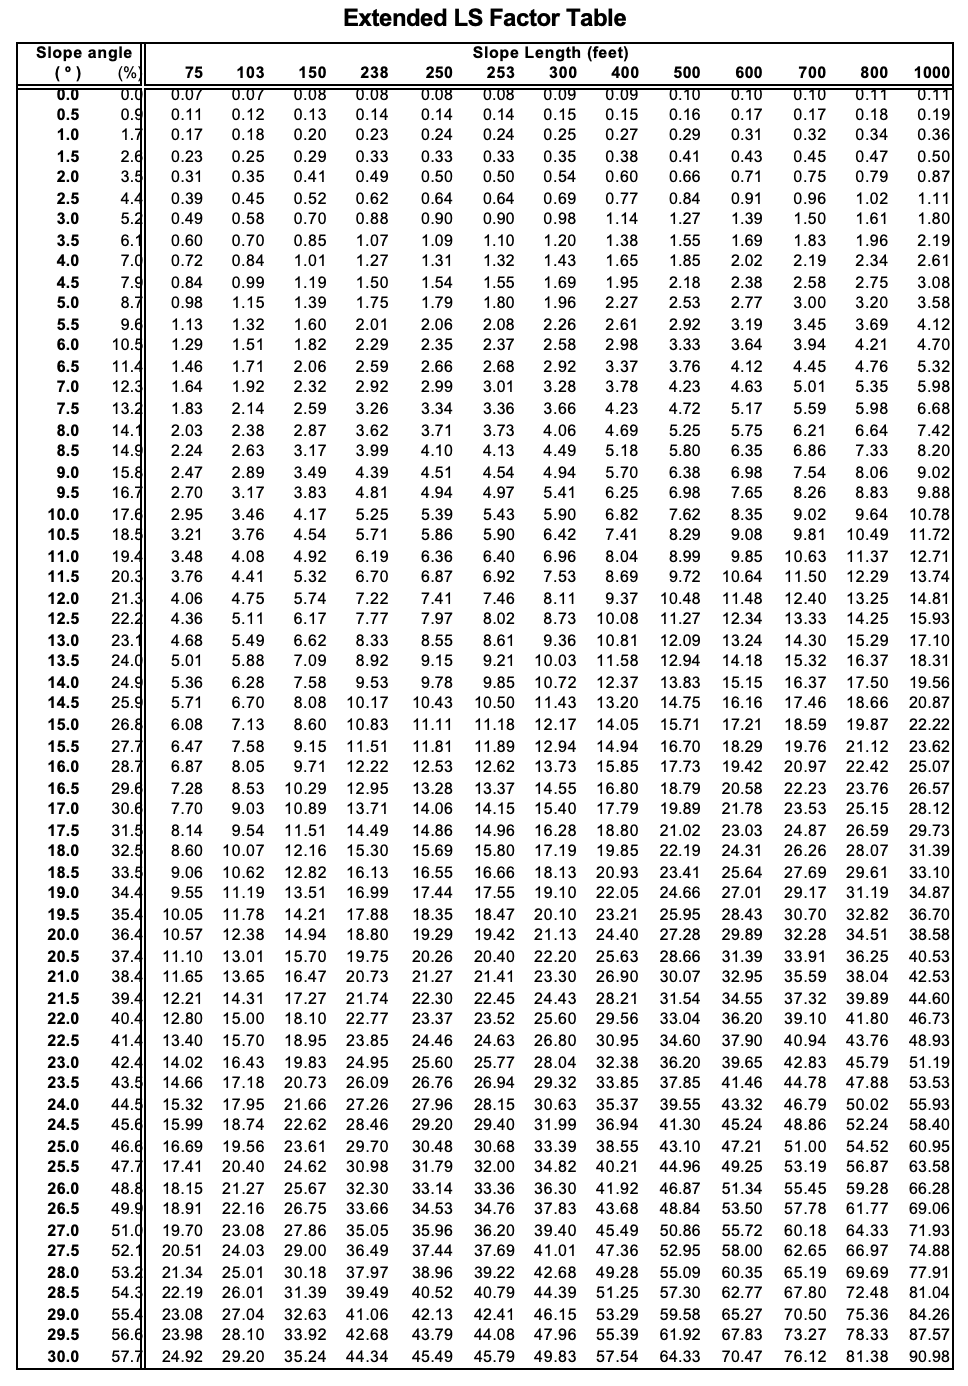
\includegraphics{extended-ls-factor-table.png}

}

\caption{\label{fig-ls}Extended LS Factor Table. Use values from steps
3b and 3d.}

\end{figure}

\hypertarget{investigation-d-modifying-soil-loss}{%
\section{INVESTIGATION D: Modifying Soil
Loss}\label{investigation-d-modifying-soil-loss}}

The tolerable soil loss for most soils in Minnesota is approximately 3
to 5 tons per acre per year. Which area(s) from Table 1 in Investigation
C exceed T (circle two)?

\textbf{Site 1}
~~~~~~~~~~~~~~~~~~~~~~~~~~~~~~~~~~~~~~~~~~~~~\textbf{Site 2} ~~~~~~
~~~~~~~~~~~~~~~~~~~~~~~~~~~~~~~~~~~~~~~\textbf{Site 3}

Modify C and P to reduce erosion below T for the areas you circled. Fill
out the tables below.

Keep in mind that the landowner wants to maximize their income from the
land while implementing conservation practices. Converting a field to
woodland significantly reduces income and requires ten to twenty years'
investment before realizing any return. Consequently, converting a field
to woodland is the least desirable option and should be used only if no
other combination to reduce A to below T can be found.

Fill out the table with your new management strategy.

 
  \providecommand{\huxb}[2]{\arrayrulecolor[RGB]{#1}\global\arrayrulewidth=#2pt}
  \providecommand{\huxvb}[2]{\color[RGB]{#1}\vrule width #2pt}
  \providecommand{\huxtpad}[1]{\rule{0pt}{#1}}
  \providecommand{\huxbpad}[1]{\rule[-#1]{0pt}{#1}}

\begin{table}[h!]
\begin{centerbox}
\begin{threeparttable}
 
\setlength{\tabcolsep}{0pt}
\begin{tabularx}{0.9\textwidth}{p{0.3\textwidth} p{0.3\textwidth} p{0.3\textwidth}}


\hhline{>{\huxb{0, 0, 0}{1}}->{\huxb{0, 0, 0}{1}}->{\huxb{0, 0, 0}{1}}-}
\arrayrulecolor{black}

\multicolumn{1}{!{\huxvb{0, 0, 0}{1}}m{0.3\textwidth}!{\huxvb{0, 0, 0}{1}}}{\hspace{0pt}\parbox[c]{0.3\textwidth-0pt-4pt}{\huxtpad{0pt + 1em}\centering \textbf{Site}\huxbpad{4pt}}} &
\multicolumn{1}{m{0.3\textwidth}!{\huxvb{0, 0, 0}{1}}}{\hspace{4pt}\parbox[c]{0.3\textwidth-4pt-4pt}{\huxtpad{0pt + 1em}\centering \textbf{C}\huxbpad{4pt}}} &
\multicolumn{1}{m{0.3\textwidth}!{\huxvb{0, 0, 0}{1}}}{\hspace{4pt}\parbox[c]{0.3\textwidth-4pt-0pt}{\huxtpad{0pt + 1em}\centering \textbf{P}\huxbpad{4pt}}} \tabularnewline[-0.5pt]


\hhline{>{\huxb{0, 0, 0}{1}}->{\huxb{0, 0, 0}{1}}->{\huxb{0, 0, 0}{1}}-}
\arrayrulecolor{black}

\multicolumn{1}{!{\huxvb{0, 0, 0}{1}}m{0.3\textwidth}!{\huxvb{0, 0, 0}{1}}}{\hspace{0pt}\parbox[c]{0.3\textwidth-0pt-4pt}{\huxtpad{20pt + 1em}\centering 1\huxbpad{20pt}}} &
\multicolumn{1}{m{0.3\textwidth}!{\huxvb{0, 0, 0}{1}}}{\hspace{4pt}\parbox[c]{0.3\textwidth-4pt-4pt}{\huxtpad{20pt + 1em}\centering \huxbpad{20pt}}} &
\multicolumn{1}{m{0.3\textwidth}!{\huxvb{0, 0, 0}{1}}}{\hspace{4pt}\parbox[c]{0.3\textwidth-4pt-0pt}{\huxtpad{20pt + 1em}\centering \huxbpad{20pt}}} \tabularnewline[-0.5pt]


\hhline{>{\huxb{0, 0, 0}{1}}->{\huxb{0, 0, 0}{1}}->{\huxb{0, 0, 0}{1}}-}
\arrayrulecolor{black}

\multicolumn{1}{!{\huxvb{0, 0, 0}{1}}m{0.3\textwidth}!{\huxvb{0, 0, 0}{1}}}{\hspace{0pt}\parbox[c]{0.3\textwidth-0pt-4pt}{\huxtpad{20pt + 1em}\centering 2\huxbpad{20pt}}} &
\multicolumn{1}{m{0.3\textwidth}!{\huxvb{0, 0, 0}{1}}}{\hspace{4pt}\parbox[c]{0.3\textwidth-4pt-4pt}{\huxtpad{20pt + 1em}\centering \huxbpad{20pt}}} &
\multicolumn{1}{m{0.3\textwidth}!{\huxvb{0, 0, 0}{1}}}{\hspace{4pt}\parbox[c]{0.3\textwidth-4pt-0pt}{\huxtpad{20pt + 1em}\centering \huxbpad{20pt}}} \tabularnewline[-0.5pt]


\hhline{>{\huxb{0, 0, 0}{1}}->{\huxb{0, 0, 0}{1}}->{\huxb{0, 0, 0}{1}}-}
\arrayrulecolor{black}

\multicolumn{1}{!{\huxvb{0, 0, 0}{1}}m{0.3\textwidth}!{\huxvb{0, 0, 0}{1}}}{\hspace{0pt}\parbox[c]{0.3\textwidth-0pt-4pt}{\huxtpad{20pt + 1em}\centering 3\huxbpad{20pt}}} &
\multicolumn{1}{m{0.3\textwidth}!{\huxvb{0, 0, 0}{1}}}{\hspace{4pt}\parbox[c]{0.3\textwidth-4pt-4pt}{\huxtpad{20pt + 1em}\centering \huxbpad{20pt}}} &
\multicolumn{1}{m{0.3\textwidth}!{\huxvb{0, 0, 0}{1}}}{\hspace{4pt}\parbox[c]{0.3\textwidth-4pt-0pt}{\huxtpad{20pt + 1em}\centering \huxbpad{20pt}}} \tabularnewline[-0.5pt]


\hhline{>{\huxb{0, 0, 0}{1}}->{\huxb{0, 0, 0}{1}}->{\huxb{0, 0, 0}{1}}-}
\arrayrulecolor{black}
\end{tabularx}
\end{threeparttable}\par\end{centerbox}

\end{table}
 

Show new calculations in the table below.

 
  \providecommand{\huxb}[2]{\arrayrulecolor[RGB]{#1}\global\arrayrulewidth=#2pt}
  \providecommand{\huxvb}[2]{\color[RGB]{#1}\vrule width #2pt}
  \providecommand{\huxtpad}[1]{\rule{0pt}{#1}}
  \providecommand{\huxbpad}[1]{\rule[-#1]{0pt}{#1}}

\begin{table}[h!]
\begin{centerbox}
\begin{threeparttable}
 
\setlength{\tabcolsep}{0pt}
\begin{tabularx}{0.9\textwidth}{p{0.1125\textwidth} p{0.1125\textwidth} p{0.1125\textwidth} p{0.1125\textwidth} p{0.1125\textwidth} p{0.1125\textwidth} p{0.1125\textwidth} p{0.1125\textwidth}}


\hhline{>{\huxb{0, 0, 0}{1}}->{\huxb{0, 0, 0}{1}}->{\huxb{0, 0, 0}{1}}->{\huxb{0, 0, 0}{1}}->{\huxb{0, 0, 0}{1}}->{\huxb{0, 0, 0}{1}}->{\huxb{0, 0, 0}{1}}->{\huxb{0, 0, 0}{1}}-}
\arrayrulecolor{black}

\multicolumn{1}{!{\huxvb{0, 0, 0}{1}}m{0.1125\textwidth}!{\huxvb{0, 0, 0}{1}}}{\hspace{0pt}\parbox[c]{0.1125\textwidth-0pt-4pt}{\huxtpad{0pt + 1em}\centering \textbf{}\huxbpad{4pt}}} &
\multicolumn{1}{m{0.1125\textwidth}!{\huxvb{0, 0, 0}{1}}}{\hspace{4pt}\parbox[c]{0.1125\textwidth-4pt-4pt}{\huxtpad{0pt + 1em}\centering \textbf{R}\huxbpad{4pt}}} &
\multicolumn{1}{m{0.1125\textwidth}!{\huxvb{0, 0, 0}{1}}}{\hspace{4pt}\parbox[c]{0.1125\textwidth-4pt-4pt}{\huxtpad{0pt + 1em}\centering \textbf{K}\huxbpad{4pt}}} &
\multicolumn{1}{m{0.1125\textwidth}!{\huxvb{0, 0, 0}{1}}}{\hspace{4pt}\parbox[c]{0.1125\textwidth-4pt-4pt}{\huxtpad{0pt + 1em}\centering \textbf{LS}\huxbpad{4pt}}} &
\multicolumn{1}{m{0.1125\textwidth}!{\huxvb{0, 0, 0}{1}}}{\hspace{4pt}\parbox[c]{0.1125\textwidth-4pt-4pt}{\huxtpad{0pt + 1em}\centering \textbf{C}\huxbpad{4pt}}} &
\multicolumn{1}{m{0.1125\textwidth}!{\huxvb{0, 0, 0}{1}}}{\hspace{4pt}\parbox[c]{0.1125\textwidth-4pt-4pt}{\huxtpad{0pt + 1em}\centering \textbf{P}\huxbpad{4pt}}} &
\multicolumn{1}{m{0.1125\textwidth}!{\huxvb{0, 0, 0}{1}}}{\hspace{4pt}\parbox[c]{0.1125\textwidth-4pt-4pt}{\huxtpad{0pt + 1em}\centering \textbf{New A}\huxbpad{4pt}}} &
\multicolumn{1}{m{0.1125\textwidth}!{\huxvb{0, 0, 0}{1}}}{\hspace{4pt}\parbox[c]{0.1125\textwidth-4pt-0pt}{\huxtpad{0pt + 1em}\centering \textbf{T}\huxbpad{4pt}}} \tabularnewline[-0.5pt]


\hhline{>{\huxb{0, 0, 0}{1}}->{\huxb{0, 0, 0}{1}}->{\huxb{0, 0, 0}{1}}->{\huxb{0, 0, 0}{1}}->{\huxb{0, 0, 0}{1}}->{\huxb{0, 0, 0}{1}}->{\huxb{0, 0, 0}{1}}->{\huxb{0, 0, 0}{1}}-}
\arrayrulecolor{black}

\multicolumn{1}{!{\huxvb{0, 0, 0}{1}}m{0.1125\textwidth}!{\huxvb{0, 0, 0}{1}}}{\hspace{0pt}\parbox[c]{0.1125\textwidth-0pt-4pt}{\huxtpad{4pt + 1em}\centering 1\huxbpad{4pt}}} &
\multicolumn{1}{m{0.1125\textwidth}!{\huxvb{0, 0, 0}{1}}}{\hspace{4pt}\parbox[c]{0.1125\textwidth-4pt-4pt}{\huxtpad{4pt + 1em}\centering \huxbpad{4pt}}} &
\multicolumn{1}{m{0.1125\textwidth}!{\huxvb{0, 0, 0}{1}}}{\hspace{4pt}\parbox[c]{0.1125\textwidth-4pt-4pt}{\huxtpad{4pt + 1em}\centering \huxbpad{4pt}}} &
\multicolumn{1}{m{0.1125\textwidth}!{\huxvb{0, 0, 0}{1}}}{\hspace{4pt}\parbox[c]{0.1125\textwidth-4pt-4pt}{\huxtpad{4pt + 1em}\centering \huxbpad{4pt}}} &
\multicolumn{1}{m{0.1125\textwidth}!{\huxvb{0, 0, 0}{1}}}{\hspace{4pt}\parbox[c]{0.1125\textwidth-4pt-4pt}{\huxtpad{4pt + 1em}\centering \huxbpad{4pt}}} &
\multicolumn{1}{m{0.1125\textwidth}!{\huxvb{0, 0, 0}{1}}}{\hspace{4pt}\parbox[c]{0.1125\textwidth-4pt-4pt}{\huxtpad{4pt + 1em}\centering \huxbpad{4pt}}} &
\multicolumn{1}{m{0.1125\textwidth}!{\huxvb{0, 0, 0}{1}}}{\hspace{4pt}\parbox[c]{0.1125\textwidth-4pt-4pt}{\huxtpad{4pt + 1em}\centering \huxbpad{4pt}}} &
\multicolumn{1}{m{0.1125\textwidth}!{\huxvb{0, 0, 0}{1}}}{\hspace{4pt}\parbox[c]{0.1125\textwidth-4pt-0pt}{\huxtpad{4pt + 1em}\centering \huxbpad{4pt}}} \tabularnewline[-0.5pt]


\hhline{>{\huxb{0, 0, 0}{1}}->{\huxb{0, 0, 0}{1}}->{\huxb{0, 0, 0}{1}}->{\huxb{0, 0, 0}{1}}->{\huxb{0, 0, 0}{1}}->{\huxb{0, 0, 0}{1}}->{\huxb{0, 0, 0}{1}}->{\huxb{0, 0, 0}{1}}-}
\arrayrulecolor{black}

\multicolumn{1}{!{\huxvb{0, 0, 0}{1}}m{0.1125\textwidth}!{\huxvb{0, 0, 0}{1}}}{\hspace{0pt}\parbox[c]{0.1125\textwidth-0pt-4pt}{\huxtpad{4pt + 1em}\centering 2\huxbpad{4pt}}} &
\multicolumn{1}{m{0.1125\textwidth}!{\huxvb{0, 0, 0}{1}}}{\hspace{4pt}\parbox[c]{0.1125\textwidth-4pt-4pt}{\huxtpad{4pt + 1em}\centering \huxbpad{4pt}}} &
\multicolumn{1}{m{0.1125\textwidth}!{\huxvb{0, 0, 0}{1}}}{\hspace{4pt}\parbox[c]{0.1125\textwidth-4pt-4pt}{\huxtpad{4pt + 1em}\centering \huxbpad{4pt}}} &
\multicolumn{1}{m{0.1125\textwidth}!{\huxvb{0, 0, 0}{1}}}{\hspace{4pt}\parbox[c]{0.1125\textwidth-4pt-4pt}{\huxtpad{4pt + 1em}\centering \huxbpad{4pt}}} &
\multicolumn{1}{m{0.1125\textwidth}!{\huxvb{0, 0, 0}{1}}}{\hspace{4pt}\parbox[c]{0.1125\textwidth-4pt-4pt}{\huxtpad{4pt + 1em}\centering \huxbpad{4pt}}} &
\multicolumn{1}{m{0.1125\textwidth}!{\huxvb{0, 0, 0}{1}}}{\hspace{4pt}\parbox[c]{0.1125\textwidth-4pt-4pt}{\huxtpad{4pt + 1em}\centering \huxbpad{4pt}}} &
\multicolumn{1}{m{0.1125\textwidth}!{\huxvb{0, 0, 0}{1}}}{\hspace{4pt}\parbox[c]{0.1125\textwidth-4pt-4pt}{\huxtpad{4pt + 1em}\centering \huxbpad{4pt}}} &
\multicolumn{1}{m{0.1125\textwidth}!{\huxvb{0, 0, 0}{1}}}{\hspace{4pt}\parbox[c]{0.1125\textwidth-4pt-0pt}{\huxtpad{4pt + 1em}\centering \huxbpad{4pt}}} \tabularnewline[-0.5pt]


\hhline{>{\huxb{0, 0, 0}{1}}->{\huxb{0, 0, 0}{1}}->{\huxb{0, 0, 0}{1}}->{\huxb{0, 0, 0}{1}}->{\huxb{0, 0, 0}{1}}->{\huxb{0, 0, 0}{1}}->{\huxb{0, 0, 0}{1}}->{\huxb{0, 0, 0}{1}}-}
\arrayrulecolor{black}

\multicolumn{1}{!{\huxvb{0, 0, 0}{1}}m{0.1125\textwidth}!{\huxvb{0, 0, 0}{1}}}{\hspace{0pt}\parbox[c]{0.1125\textwidth-0pt-4pt}{\huxtpad{4pt + 1em}\centering 3\huxbpad{0pt}}} &
\multicolumn{1}{m{0.1125\textwidth}!{\huxvb{0, 0, 0}{1}}}{\hspace{4pt}\parbox[c]{0.1125\textwidth-4pt-4pt}{\huxtpad{4pt + 1em}\centering \huxbpad{0pt}}} &
\multicolumn{1}{m{0.1125\textwidth}!{\huxvb{0, 0, 0}{1}}}{\hspace{4pt}\parbox[c]{0.1125\textwidth-4pt-4pt}{\huxtpad{4pt + 1em}\centering \huxbpad{0pt}}} &
\multicolumn{1}{m{0.1125\textwidth}!{\huxvb{0, 0, 0}{1}}}{\hspace{4pt}\parbox[c]{0.1125\textwidth-4pt-4pt}{\huxtpad{4pt + 1em}\centering \huxbpad{0pt}}} &
\multicolumn{1}{m{0.1125\textwidth}!{\huxvb{0, 0, 0}{1}}}{\hspace{4pt}\parbox[c]{0.1125\textwidth-4pt-4pt}{\huxtpad{4pt + 1em}\centering \huxbpad{0pt}}} &
\multicolumn{1}{m{0.1125\textwidth}!{\huxvb{0, 0, 0}{1}}}{\hspace{4pt}\parbox[c]{0.1125\textwidth-4pt-4pt}{\huxtpad{4pt + 1em}\centering \huxbpad{0pt}}} &
\multicolumn{1}{m{0.1125\textwidth}!{\huxvb{0, 0, 0}{1}}}{\hspace{4pt}\parbox[c]{0.1125\textwidth-4pt-4pt}{\huxtpad{4pt + 1em}\centering \huxbpad{0pt}}} &
\multicolumn{1}{m{0.1125\textwidth}!{\huxvb{0, 0, 0}{1}}}{\hspace{4pt}\parbox[c]{0.1125\textwidth-4pt-0pt}{\huxtpad{4pt + 1em}\centering \huxbpad{0pt}}} \tabularnewline[-0.5pt]


\hhline{>{\huxb{0, 0, 0}{1}}->{\huxb{0, 0, 0}{1}}->{\huxb{0, 0, 0}{1}}->{\huxb{0, 0, 0}{1}}->{\huxb{0, 0, 0}{1}}->{\huxb{0, 0, 0}{1}}->{\huxb{0, 0, 0}{1}}->{\huxb{0, 0, 0}{1}}-}
\arrayrulecolor{black}
\end{tabularx}
\end{threeparttable}\par\end{centerbox}

\end{table}
 

Crop management factor, \textbf{C}.

 
  \providecommand{\huxb}[2]{\arrayrulecolor[RGB]{#1}\global\arrayrulewidth=#2pt}
  \providecommand{\huxvb}[2]{\color[RGB]{#1}\vrule width #2pt}
  \providecommand{\huxtpad}[1]{\rule{0pt}{#1}}
  \providecommand{\huxbpad}[1]{\rule[-#1]{0pt}{#1}}

\begin{table}[h!]
\begin{centerbox}
\begin{threeparttable}
 
\setlength{\tabcolsep}{0pt}
\begin{tabularx}{0.9\textwidth}{p{0.45\textwidth} p{0.45\textwidth}}


\hhline{>{\huxb{0, 0, 0}{1}}->{\huxb{0, 0, 0}{1}}-}
\arrayrulecolor{black}

\multicolumn{1}{!{\huxvb{0, 0, 0}{1}}m{0.45\textwidth}!{\huxvb{0, 0, 0}{1}}}{\hspace{0pt}\parbox[c]{0.45\textwidth-0pt-4pt}{\huxtpad{0pt + 1em}\centering \textbf{C}\huxbpad{4pt}}} &
\multicolumn{1}{m{0.45\textwidth}!{\huxvb{0, 0, 0}{1}}}{\hspace{4pt}\parbox[c]{0.45\textwidth-4pt-0pt}{\huxtpad{0pt + 1em}\centering \textbf{Management}\huxbpad{4pt}}} \tabularnewline[-0.5pt]


\hhline{>{\huxb{0, 0, 0}{1}}->{\huxb{0, 0, 0}{1}}-}
\arrayrulecolor{black}

\multicolumn{1}{!{\huxvb{0, 0, 0}{1}}m{0.45\textwidth}!{\huxvb{0, 0, 0}{1}}}{\hspace{0pt}\parbox[c]{0.45\textwidth-0pt-4pt}{\huxtpad{4pt + 1em}\centering 1.00\huxbpad{4pt}}} &
\multicolumn{1}{m{0.45\textwidth}!{\huxvb{0, 0, 0}{1}}}{\hspace{4pt}\parbox[c]{0.45\textwidth-4pt-0pt}{\huxtpad{4pt + 1em}\centering No crop; moldboard plow\huxbpad{4pt}}} \tabularnewline[-0.5pt]


\hhline{>{\huxb{0, 0, 0}{1}}->{\huxb{0, 0, 0}{1}}-}
\arrayrulecolor{black}

\multicolumn{1}{!{\huxvb{0, 0, 0}{1}}m{0.45\textwidth}!{\huxvb{0, 0, 0}{1}}}{\hspace{0pt}\parbox[c]{0.45\textwidth-0pt-4pt}{\huxtpad{4pt + 1em}\centering 0.55\huxbpad{4pt}}} &
\multicolumn{1}{m{0.45\textwidth}!{\huxvb{0, 0, 0}{1}}}{\hspace{4pt}\parbox[c]{0.45\textwidth-4pt-0pt}{\huxtpad{4pt + 1em}\centering Continuous corn; moldboard plow\huxbpad{4pt}}} \tabularnewline[-0.5pt]


\hhline{>{\huxb{0, 0, 0}{1}}->{\huxb{0, 0, 0}{1}}-}
\arrayrulecolor{black}

\multicolumn{1}{!{\huxvb{0, 0, 0}{1}}m{0.45\textwidth}!{\huxvb{0, 0, 0}{1}}}{\hspace{0pt}\parbox[c]{0.45\textwidth-0pt-4pt}{\huxtpad{4pt + 1em}\centering 0.40\huxbpad{4pt}}} &
\multicolumn{1}{m{0.45\textwidth}!{\huxvb{0, 0, 0}{1}}}{\hspace{4pt}\parbox[c]{0.45\textwidth-4pt-0pt}{\huxtpad{4pt + 1em}\centering Corn-soybean rotation\huxbpad{4pt}}} \tabularnewline[-0.5pt]


\hhline{>{\huxb{0, 0, 0}{1}}->{\huxb{0, 0, 0}{1}}-}
\arrayrulecolor{black}

\multicolumn{1}{!{\huxvb{0, 0, 0}{1}}m{0.45\textwidth}!{\huxvb{0, 0, 0}{1}}}{\hspace{0pt}\parbox[c]{0.45\textwidth-0pt-4pt}{\huxtpad{4pt + 1em}\centering 0.30\huxbpad{4pt}}} &
\multicolumn{1}{m{0.45\textwidth}!{\huxvb{0, 0, 0}{1}}}{\hspace{4pt}\parbox[c]{0.45\textwidth-4pt-0pt}{\huxtpad{4pt + 1em}\centering Continuous corn; conservation tillage\huxbpad{4pt}}} \tabularnewline[-0.5pt]


\hhline{>{\huxb{0, 0, 0}{1}}->{\huxb{0, 0, 0}{1}}-}
\arrayrulecolor{black}

\multicolumn{1}{!{\huxvb{0, 0, 0}{1}}m{0.45\textwidth}!{\huxvb{0, 0, 0}{1}}}{\hspace{0pt}\parbox[c]{0.45\textwidth-0pt-4pt}{\huxtpad{4pt + 1em}\centering 0.20\huxbpad{4pt}}} &
\multicolumn{1}{m{0.45\textwidth}!{\huxvb{0, 0, 0}{1}}}{\hspace{4pt}\parbox[c]{0.45\textwidth-4pt-0pt}{\huxtpad{4pt + 1em}\centering Corn-oats rotation\huxbpad{4pt}}} \tabularnewline[-0.5pt]


\hhline{>{\huxb{0, 0, 0}{1}}->{\huxb{0, 0, 0}{1}}-}
\arrayrulecolor{black}

\multicolumn{1}{!{\huxvb{0, 0, 0}{1}}m{0.45\textwidth}!{\huxvb{0, 0, 0}{1}}}{\hspace{0pt}\parbox[c]{0.45\textwidth-0pt-4pt}{\huxtpad{4pt + 1em}\centering 0.08\huxbpad{4pt}}} &
\multicolumn{1}{m{0.45\textwidth}!{\huxvb{0, 0, 0}{1}}}{\hspace{4pt}\parbox[c]{0.45\textwidth-4pt-0pt}{\huxtpad{4pt + 1em}\centering Corn-oats-pasture rotation\huxbpad{4pt}}} \tabularnewline[-0.5pt]


\hhline{>{\huxb{0, 0, 0}{1}}->{\huxb{0, 0, 0}{1}}-}
\arrayrulecolor{black}

\multicolumn{1}{!{\huxvb{0, 0, 0}{1}}m{0.45\textwidth}!{\huxvb{0, 0, 0}{1}}}{\hspace{0pt}\parbox[c]{0.45\textwidth-0pt-4pt}{\huxtpad{4pt + 1em}\centering 0.04\huxbpad{4pt}}} &
\multicolumn{1}{m{0.45\textwidth}!{\huxvb{0, 0, 0}{1}}}{\hspace{4pt}\parbox[c]{0.45\textwidth-4pt-0pt}{\huxtpad{4pt + 1em}\centering Continuous corn; no till\huxbpad{4pt}}} \tabularnewline[-0.5pt]


\hhline{>{\huxb{0, 0, 0}{1}}->{\huxb{0, 0, 0}{1}}-}
\arrayrulecolor{black}

\multicolumn{1}{!{\huxvb{0, 0, 0}{1}}m{0.45\textwidth}!{\huxvb{0, 0, 0}{1}}}{\hspace{0pt}\parbox[c]{0.45\textwidth-0pt-4pt}{\huxtpad{4pt + 1em}\centering 0.01\huxbpad{4pt}}} &
\multicolumn{1}{m{0.45\textwidth}!{\huxvb{0, 0, 0}{1}}}{\hspace{4pt}\parbox[c]{0.45\textwidth-4pt-0pt}{\huxtpad{4pt + 1em}\centering Pasture\huxbpad{4pt}}} \tabularnewline[-0.5pt]


\hhline{>{\huxb{0, 0, 0}{1}}->{\huxb{0, 0, 0}{1}}-}
\arrayrulecolor{black}

\multicolumn{1}{!{\huxvb{0, 0, 0}{1}}m{0.45\textwidth}!{\huxvb{0, 0, 0}{1}}}{\hspace{0pt}\parbox[c]{0.45\textwidth-0pt-4pt}{\huxtpad{4pt + 1em}\centering 0.00\huxbpad{0pt}}} &
\multicolumn{1}{m{0.45\textwidth}!{\huxvb{0, 0, 0}{1}}}{\hspace{4pt}\parbox[c]{0.45\textwidth-4pt-0pt}{\huxtpad{4pt + 1em}\centering Woodland\huxbpad{0pt}}} \tabularnewline[-0.5pt]


\hhline{>{\huxb{0, 0, 0}{1}}->{\huxb{0, 0, 0}{1}}-}
\arrayrulecolor{black}
\end{tabularx}
\end{threeparttable}\par\end{centerbox}

\end{table}
 

Erosion control practice factor, ratio of soil loss compared to farming
up and down the slope, \textbf{P}.

 
  \providecommand{\huxb}[2]{\arrayrulecolor[RGB]{#1}\global\arrayrulewidth=#2pt}
  \providecommand{\huxvb}[2]{\color[RGB]{#1}\vrule width #2pt}
  \providecommand{\huxtpad}[1]{\rule{0pt}{#1}}
  \providecommand{\huxbpad}[1]{\rule[-#1]{0pt}{#1}}

\begin{table}[h!]
\begin{centerbox}
\begin{threeparttable}
 
\setlength{\tabcolsep}{0pt}
\begin{tabularx}{0.9\textwidth}{p{0.18\textwidth} p{0.18\textwidth} p{0.18\textwidth} p{0.18\textwidth} p{0.18\textwidth}}


\hhline{>{\huxb{0, 0, 0}{1}}->{\huxb{0, 0, 0}{1}}->{\huxb{0, 0, 0}{1}}->{\huxb{0, 0, 0}{1}}->{\huxb{0, 0, 0}{1}}-}
\arrayrulecolor{black}

\multicolumn{1}{!{\huxvb{0, 0, 0}{1}}m{0.18\textwidth}!{\huxvb{0, 0, 0}{1}}}{\hspace{0pt}\parbox[c]{0.18\textwidth-0pt-4pt}{\huxtpad{0pt + 1em}\centering \textbf{Slope \%}\huxbpad{4pt}}} &
\multicolumn{1}{m{0.18\textwidth}!{\huxvb{0, 0, 0}{1}}}{\hspace{4pt}\parbox[c]{0.18\textwidth-4pt-4pt}{\huxtpad{0pt + 1em}\centering \textbf{No Practice}\huxbpad{4pt}}} &
\multicolumn{1}{m{0.18\textwidth}!{\huxvb{0, 0, 0}{1}}}{\hspace{4pt}\parbox[c]{0.18\textwidth-4pt-4pt}{\huxtpad{0pt + 1em}\centering \textbf{Contouring Alone}\huxbpad{4pt}}} &
\multicolumn{1}{m{0.18\textwidth}!{\huxvb{0, 0, 0}{1}}}{\hspace{4pt}\parbox[c]{0.18\textwidth-4pt-4pt}{\huxtpad{0pt + 1em}\centering \textbf{Contouring plus alternate strips with small grains}\huxbpad{4pt}}} &
\multicolumn{1}{m{0.18\textwidth}!{\huxvb{0, 0, 0}{1}}}{\hspace{4pt}\parbox[c]{0.18\textwidth-4pt-0pt}{\huxtpad{0pt + 1em}\centering \textbf{Contouring plus alternate strips with grass}\huxbpad{4pt}}} \tabularnewline[-0.5pt]


\hhline{>{\huxb{0, 0, 0}{1}}->{\huxb{0, 0, 0}{1}}->{\huxb{0, 0, 0}{1}}->{\huxb{0, 0, 0}{1}}->{\huxb{0, 0, 0}{1}}-}
\arrayrulecolor{black}

\multicolumn{1}{!{\huxvb{0, 0, 0}{1}}m{0.18\textwidth}!{\huxvb{0, 0, 0}{1}}}{\hspace{0pt}\parbox[c]{0.18\textwidth-0pt-4pt}{\huxtpad{4pt + 1em}\centering 1.1-2.0\huxbpad{4pt}}} &
\multicolumn{1}{m{0.18\textwidth}!{\huxvb{0, 0, 0}{1}}}{\hspace{4pt}\parbox[c]{0.18\textwidth-4pt-4pt}{\huxtpad{4pt + 1em}\centering 1.0\huxbpad{4pt}}} &
\multicolumn{1}{m{0.18\textwidth}!{\huxvb{0, 0, 0}{1}}}{\hspace{4pt}\parbox[c]{0.18\textwidth-4pt-4pt}{\huxtpad{4pt + 1em}\centering 0.6\huxbpad{4pt}}} &
\multicolumn{1}{m{0.18\textwidth}!{\huxvb{0, 0, 0}{1}}}{\hspace{4pt}\parbox[c]{0.18\textwidth-4pt-4pt}{\huxtpad{4pt + 1em}\centering 0.4\huxbpad{4pt}}} &
\multicolumn{1}{m{0.18\textwidth}!{\huxvb{0, 0, 0}{1}}}{\hspace{4pt}\parbox[c]{0.18\textwidth-4pt-0pt}{\huxtpad{4pt + 1em}\centering 0.3\huxbpad{4pt}}} \tabularnewline[-0.5pt]


\hhline{>{\huxb{0, 0, 0}{1}}->{\huxb{0, 0, 0}{1}}->{\huxb{0, 0, 0}{1}}->{\huxb{0, 0, 0}{1}}->{\huxb{0, 0, 0}{1}}-}
\arrayrulecolor{black}

\multicolumn{1}{!{\huxvb{0, 0, 0}{1}}m{0.18\textwidth}!{\huxvb{0, 0, 0}{1}}}{\hspace{0pt}\parbox[c]{0.18\textwidth-0pt-4pt}{\huxtpad{4pt + 1em}\centering 2.1-7.0\huxbpad{4pt}}} &
\multicolumn{1}{m{0.18\textwidth}!{\huxvb{0, 0, 0}{1}}}{\hspace{4pt}\parbox[c]{0.18\textwidth-4pt-4pt}{\huxtpad{4pt + 1em}\centering 1.0\huxbpad{4pt}}} &
\multicolumn{1}{m{0.18\textwidth}!{\huxvb{0, 0, 0}{1}}}{\hspace{4pt}\parbox[c]{0.18\textwidth-4pt-4pt}{\huxtpad{4pt + 1em}\centering 0.5\huxbpad{4pt}}} &
\multicolumn{1}{m{0.18\textwidth}!{\huxvb{0, 0, 0}{1}}}{\hspace{4pt}\parbox[c]{0.18\textwidth-4pt-4pt}{\huxtpad{4pt + 1em}\centering 0.4\huxbpad{4pt}}} &
\multicolumn{1}{m{0.18\textwidth}!{\huxvb{0, 0, 0}{1}}}{\hspace{4pt}\parbox[c]{0.18\textwidth-4pt-0pt}{\huxtpad{4pt + 1em}\centering 0.2\huxbpad{4pt}}} \tabularnewline[-0.5pt]


\hhline{>{\huxb{0, 0, 0}{1}}->{\huxb{0, 0, 0}{1}}->{\huxb{0, 0, 0}{1}}->{\huxb{0, 0, 0}{1}}->{\huxb{0, 0, 0}{1}}-}
\arrayrulecolor{black}

\multicolumn{1}{!{\huxvb{0, 0, 0}{1}}m{0.18\textwidth}!{\huxvb{0, 0, 0}{1}}}{\hspace{0pt}\parbox[c]{0.18\textwidth-0pt-4pt}{\huxtpad{4pt + 1em}\centering 7.1-12.0\huxbpad{4pt}}} &
\multicolumn{1}{m{0.18\textwidth}!{\huxvb{0, 0, 0}{1}}}{\hspace{4pt}\parbox[c]{0.18\textwidth-4pt-4pt}{\huxtpad{4pt + 1em}\centering 1.0\huxbpad{4pt}}} &
\multicolumn{1}{m{0.18\textwidth}!{\huxvb{0, 0, 0}{1}}}{\hspace{4pt}\parbox[c]{0.18\textwidth-4pt-4pt}{\huxtpad{4pt + 1em}\centering 0.6\huxbpad{4pt}}} &
\multicolumn{1}{m{0.18\textwidth}!{\huxvb{0, 0, 0}{1}}}{\hspace{4pt}\parbox[c]{0.18\textwidth-4pt-4pt}{\huxtpad{4pt + 1em}\centering 0.4\huxbpad{4pt}}} &
\multicolumn{1}{m{0.18\textwidth}!{\huxvb{0, 0, 0}{1}}}{\hspace{4pt}\parbox[c]{0.18\textwidth-4pt-0pt}{\huxtpad{4pt + 1em}\centering 0.3\huxbpad{4pt}}} \tabularnewline[-0.5pt]


\hhline{>{\huxb{0, 0, 0}{1}}->{\huxb{0, 0, 0}{1}}->{\huxb{0, 0, 0}{1}}->{\huxb{0, 0, 0}{1}}->{\huxb{0, 0, 0}{1}}-}
\arrayrulecolor{black}

\multicolumn{1}{!{\huxvb{0, 0, 0}{1}}m{0.18\textwidth}!{\huxvb{0, 0, 0}{1}}}{\hspace{0pt}\parbox[c]{0.18\textwidth-0pt-4pt}{\huxtpad{4pt + 1em}\centering 12.1-18.0\huxbpad{4pt}}} &
\multicolumn{1}{m{0.18\textwidth}!{\huxvb{0, 0, 0}{1}}}{\hspace{4pt}\parbox[c]{0.18\textwidth-4pt-4pt}{\huxtpad{4pt + 1em}\centering 1.0\huxbpad{4pt}}} &
\multicolumn{1}{m{0.18\textwidth}!{\huxvb{0, 0, 0}{1}}}{\hspace{4pt}\parbox[c]{0.18\textwidth-4pt-4pt}{\huxtpad{4pt + 1em}\centering 0.8\huxbpad{4pt}}} &
\multicolumn{1}{m{0.18\textwidth}!{\huxvb{0, 0, 0}{1}}}{\hspace{4pt}\parbox[c]{0.18\textwidth-4pt-4pt}{\huxtpad{4pt + 1em}\centering 0.6\huxbpad{4pt}}} &
\multicolumn{1}{m{0.18\textwidth}!{\huxvb{0, 0, 0}{1}}}{\hspace{4pt}\parbox[c]{0.18\textwidth-4pt-0pt}{\huxtpad{4pt + 1em}\centering 0.4\huxbpad{4pt}}} \tabularnewline[-0.5pt]


\hhline{>{\huxb{0, 0, 0}{1}}->{\huxb{0, 0, 0}{1}}->{\huxb{0, 0, 0}{1}}->{\huxb{0, 0, 0}{1}}->{\huxb{0, 0, 0}{1}}-}
\arrayrulecolor{black}

\multicolumn{1}{!{\huxvb{0, 0, 0}{1}}m{0.18\textwidth}!{\huxvb{0, 0, 0}{1}}}{\hspace{0pt}\parbox[c]{0.18\textwidth-0pt-4pt}{\huxtpad{4pt + 1em}\centering 18.1-24.0\huxbpad{0pt}}} &
\multicolumn{1}{m{0.18\textwidth}!{\huxvb{0, 0, 0}{1}}}{\hspace{4pt}\parbox[c]{0.18\textwidth-4pt-4pt}{\huxtpad{4pt + 1em}\centering 1.0\huxbpad{0pt}}} &
\multicolumn{1}{m{0.18\textwidth}!{\huxvb{0, 0, 0}{1}}}{\hspace{4pt}\parbox[c]{0.18\textwidth-4pt-4pt}{\huxtpad{4pt + 1em}\centering 0.9\huxbpad{0pt}}} &
\multicolumn{1}{m{0.18\textwidth}!{\huxvb{0, 0, 0}{1}}}{\hspace{4pt}\parbox[c]{0.18\textwidth-4pt-4pt}{\huxtpad{4pt + 1em}\centering 0.7\huxbpad{0pt}}} &
\multicolumn{1}{m{0.18\textwidth}!{\huxvb{0, 0, 0}{1}}}{\hspace{4pt}\parbox[c]{0.18\textwidth-4pt-0pt}{\huxtpad{4pt + 1em}\centering 0.4\huxbpad{0pt}}} \tabularnewline[-0.5pt]


\hhline{>{\huxb{0, 0, 0}{1}}->{\huxb{0, 0, 0}{1}}->{\huxb{0, 0, 0}{1}}->{\huxb{0, 0, 0}{1}}->{\huxb{0, 0, 0}{1}}-}
\arrayrulecolor{black}
\end{tabularx}
\end{threeparttable}\par\end{centerbox}

\end{table}
 

\bookmarksetup{startatroot}

\hypertarget{summary}{%
\chapter{Summary}\label{summary}}

In summary, this book has no content whatsoever.

\begin{Shaded}
\begin{Highlighting}[]
\DecValTok{1} \SpecialCharTok{+} \DecValTok{1}
\end{Highlighting}
\end{Shaded}

\begin{verbatim}
[1] 2
\end{verbatim}

\bookmarksetup{startatroot}

\hypertarget{references}{%
\chapter*{References}\label{references}}
\addcontentsline{toc}{chapter}{References}

\markboth{References}{References}

\hypertarget{refs}{}
\begin{CSLReferences}{0}{0}
\end{CSLReferences}


\backmatter

\end{document}
